\documentclass{report}
\usepackage{ngerman}
\usepackage{fleqn}
\usepackage{epsfig}
\usepackage{a4wide}
\usepackage{amssymb}
\usepackage{wasysym}
\usepackage{stmaryrd}
\usepackage{fancyvrb}
\usepackage{color}
\usepackage{alltt}
\usepackage{enumerate}
\usepackage{hyperref}
\usepackage[all]{hypcap}
\hypersetup{
	colorlinks = true, 
	linkcolor  = blue,
	citecolor  = red,
        filecolor  = Gold,
        urlcolor   = [rgb]{0.5, 0.1, 0.0},
	pdfborder  = {0 0 0} 
}

\usepackage{fancyhdr}
\usepackage{lastpage} 

\renewcommand*{\familydefault}{\sfdefault}

\pagestyle{fancy}

\fancyfoot[C]{--- \thepage/\pageref{LastPage}\ ---}

\fancypagestyle{plain}{%
\fancyhf{}
\fancyfoot[C]{--- \thepage/\pageref{LastPage}\ ---}
\renewcommand{\headrulewidth}{0pt}
}

\fancyheadoffset{0.1cm}
\renewcommand{\chaptermark}[1]{\markboth{\chaptername \ \thechapter.\ #1}{}}
\renewcommand{\sectionmark}[1]{\markright{\thesection. \ #1}{}}
\fancyhead[R]{\leftmark}
\fancyhead[L]{\rightmark}

\definecolor{amethyst}{rgb}{0.2, 0.4, 0.6}
\definecolor{orange}{rgb}{1, 0.9, 0.0}

\setlength{\mathindent}{1.3cm}
\setlength{\textwidth}{17cm}
\addtolength{\oddsidemargin}{-1cm}
\addtolength{\evensidemargin}{-1cm}
\addtolength{\topmargin}{-1cm}


\setlength{\mathindent}{1.3cm}
\setlength{\topsep}{0.1cm plus0.1cm minus 0.0cm}
\setlength{\partopsep}{0.0cm plus0.1cm minus 0.0cm}
\setlength{\parsep}{0.1cm plus0.1cm minus 0.0cm}
\setlength{\parskip}{0.1cm plus0.1cm minus 0.0cm}
\newfont{\chess}{chess20}
\newfont{\bigchess}{chess30}
\newcommand{\chf}{\baselineskip20pt\lineskip0pt\chess}
\newcommand{\ds}{\displaystyle}

\newtheorem{Definition}{Definition}
\newtheorem{Notation}[Definition]{Notation}
\newtheorem{Korollar}[Definition]{Korollar}
\newtheorem{Lemma}[Definition]{Lemma}
\newtheorem{Satz}[Definition]{Satz}
\newtheorem{Theorem}[Definition]{Theorem}

\title{
\epsfig{file=dhbw-logo.eps, scale=1.5}\\[0.3cm]
       Theoretical Computer Science \texttt{I}: \\[0.1cm]
       Logic               \\[0.3cm]
      --- Winter 2015/2016 ---     \\[0.3cm]
      DHBW Mannheim}
\author{Prof.~Dr.~Karl Stroetmann}
\date{\today \\[02.5cm]
\begin{minipage}[t]{1.0\linewidth}
\noindent
These lecture notes, the corresponding \LaTeX\ sources and the programs discussed in these lecture notes are available at
\\[0.2cm]
\hspace*{\fill}
\href{https://github.com/karlstroetmann/Logik}{\texttt{https://github.com/karlstroetmann/Logik}}.
\hspace*{\fill} 
\\[0.2cm]
The \href{https://github.com/karlstroetmann/Logik/blob/master/Script/logik.pdf?raw=true}{lecture notes} are
constantly revised.   Provided you have installed  \href{http://git-scm.com/download}{\texttt{git}} on your
computer, you can clone my repository using the command 
\\[0.2cm]
\hspace*{1.3cm}
\texttt{git clone https://github.com/karlstroetmann/Logik.git}.
\\[0.2cm]
Then, the repository can be updated using the command
\\[0.2cm]
\hspace*{1.3cm}
\texttt{git pull}.
\end{minipage}
}

\newcommand{\quoted}[1]{\texttt{\symbol{34}\texttt{#1}\symbol{34}}}
\newcommand{\schluss}[2]{\frac{\displaystyle\quad \rule[-6pt]{0pt}{12pt}#1 \quad}{\displaystyle\quad \rule{0pt}{10pt}#2 \quad}}
\newcommand{\bruch}[2]{\frac{\displaystyle#1}{\displaystyle #2}}
\newcommand{\vschlus}[1]{{\displaystyle\rule[-6pt]{0pt}{12pt} \atop \rule{0pt}{10pt}#1}}

\newcommand{\example}{\vspace*{0.2cm}

\noindent
\textbf{Beispiel}: \ }

\newcommand{\exampleEng}{\vspace*{0.2cm}

\noindent
\textbf{Example}: \ }

\newcommand{\examples}{\vspace*{0.2cm}

\noindent
\textbf{Beispiele}: \ }

\newcommand{\examplesEng}{\vspace*{0.2cm}

\noindent
\textbf{Examples}: \ }

\newcommand{\next}{\vspace*{0.2cm}

\noindent}

\newcommand{\remark}{\vspace*{0.2cm}

\noindent
\textbf{Bemerkung}: }

\newcommand{\remarkEng}{\vspace*{0.2cm}

\noindent
\textbf{Remark}: }


\newcounter{aufgabe}
\newcommand{\exercise}{\vspace*{0.1cm}
\stepcounter{aufgabe}

\noindent
\textbf{Aufgabe \arabic{aufgabe}}: }

\newcommand{\exerciseEng}{\vspace*{0.1cm}
\stepcounter{aufgabe}

\noindent
\textbf{Exercise \arabic{aufgabe}}: }

\newcommand{\solution}{\vspace*{0.2cm}

\noindent
\textbf{Lösung}: \ }


\newcommand{\qed}{\hspace*{\fill} $\Box$}
\newcommand{\eox}{\hspace*{\fill} $\diamond$}
\newcommand{\exend}{\hspace*{\fill} $\diamond$}
\newcommand{\setl}{\textsc{SetlX}}
\newcommand{\struct}{\mathcal{S}}
\newcommand{\FV}{\textsl{FV}}
\newcommand{\id}{\textrm{id}}
\newcommand{\dom}{\textrm{dom}}
\newcommand{\rng}{\textrm{rng}}
\newcommand{\BV}{\textsl{BV}}
\newcommand{\var}{\textsl{Var}}
\newcommand{\el}{\!\in\!}
\newcommand{\notel}{\!\not\in\!}
\newcommand{\I}{\mathcal{I}}
\newcommand{\verum}{\top}
\newcommand{\falsum}{\bot}
\newcommand{\gentzen}{\vdash}
\newcommand{\komplement}[1]{\overline{#1}}
\newcommand{\mathquote}[1]{\mbox{``}\mathtt{#1}\mbox{''}}
\newcommand{\squote}[1]{\symbol{34}\texttt{#1}\symbol{34}}

\newcommand{\circneg}{\mbox{$\bigcirc\hspace*{-0.3cm}\neg$}}
\newcommand{\circwedge}{\mbox{$\bigcirc\hspace*{-0.3cm}\wedge$}}
\newcommand{\circvee}{\mbox{$\bigcirc\hspace*{-0.3cm}\vee$}}
\newcommand{\circright}{\mbox{$\bigcirc\hspace*{-0.45cm}\rightarrow$}}
\newcommand{\circleftright}{\mbox{$\bigcirc\hspace*{-0.45cm}\leftrightarrow$}}
\newcommand{\club }{\ensuremath{\clubsuit   }}
\newcommand{\spade}{\ensuremath{\spadesuit  }}
\newcommand{\heart}{\ensuremath{\heartsuit  }}
\newcommand{\diamo}{\ensuremath{\diamondsuit}}

\newcommand{\hoare}[3]{\bigl\{#1\bigr\}\quad\texttt{#2}\quad\bigl\{#3\bigr\}}
\newcommand{\mod}{\;\texttt{\%}\;}
\newcommand{\Oh}{\mathcal{O}}


\def\pair(#1,#2){\langle #1, #2 \rangle}


%\includeonly{prolog}
%\includeonly{einleitung, grundlagen, setl, aussagenlogik, praedikatenlogik}

\begin{document}


\maketitle
\tableofcontents
\chapter{Einleitung}
In diesem einf�hrenden Kapitel m�chte ich zun�chst motivieren, warum wir in der Informatik
nicht darum herum kommen uns mit den formalen Methoden der mathematischen Logik zu besch�ftigen.
Anschlie�end gebe ich einen �berblick �ber den Rest der Vorlesung.

\section{Motivation}
Informationstechnische Systeme 
(im Folgenden kurz als IT-Systeme bezeichnet) geh�ren zu den komplexesten Systemen, die
die Menschheit je entwickelt hat.  Das l�sst sich schon an dem Aufwand erkennen,
der bei der Erstellung von IT-Systemen anf�llt.  So sind im Bereich der Telekommunikations-Industrie
IT-Projekte, bei denen mehr als 1000 Entwickler �ber mehrere Jahre zusammenarbeiten,
die Regel.  Es ist offensichtlich, dass ein Scheitern solcher Projekte mit enormen
Kosten verbunden ist.  Einige Beispiele m�gen dies verdeutlichen.
\begin{enumerate}
\item Am 9.~Juni 1996 st�rzte die Rakete Ariane 5 auf ihrem Jungfernflug ab.
      Ursache war ein Kette von Software-Fehlern:  Ein Sensor im Navigations-System
      der Ariane 5 misst die horizontale Neigung und speichert diese zun�chst als Gleitkomma-Zahl
      mit einer Genauigkeit von 64 Bit ab.  Sp�ter wird dieser Wert dann in eine 
      16 Bit Festkomma-Zahl konvertiert.
      Bei dieser Konvertierung trat ein �berlauf ein, da die zu konvertierende Zahl
      zu gro� war, um als 16 Bit Festkomma-Zahl dargestellt werden zu k�nnen.
      In der Folge gab das Navigations-System auf dem Datenbus, der dieses System mit
      der Steuerungs-Einheit verbindet, eine Fehlermeldung aus.
       Die Daten dieser Fehlermeldung wurden von der Steuerungs-Einheit als Flugdaten 
      interpretiert.  Die Steuer-Einheit leitete daraufhin eine Korrektur des
      Fluges ein, die dazu f�hrte, dass die Rakete auseinander brach und die 
      automatische Selbstzerst�rung eingeleitet werden musste.
      Die Rakete war mit 4 Satelliten beladen. Der wirtschaftliche Schaden, der durch den Verlust dieser
      Satelliten entstanden ist, lag bei mehreren 100 Millionen Dollar.
      
      Ein vollst�ndiger Bericht �ber die Ursache des Absturzes des Ariane 5 findet sich
      im Internet unter der Adresse \\[0.1cm]
      \hspace*{1.3cm} 
      \href{http://www.ima.umn.edu/~arnold/disasters/ariane5rep.html}{\texttt{http://www.ima.umn.edu/\symbol{126}arnold/disasters/ariane5rep.html}}
\item Die Therac 25 ist ein medizinisches Bestrahlungs-Ger�t, das durch 
      Software kontrolliert wird.  Durch  Fehler in dieser Software erhielten 1985
      mindestens 6 Patienten eine �berdosis an Strahlung.  Drei dieser Patienten sind an den Folgen dieser 
      �berdosierung gestorben, die anderen wurden schwer verletzt.

      Einen detailierten Bericht �ber diese Unf�lle finden Sie unter \\[0.1cm]
      \hspace*{1.3cm} 
      \href{http://courses.cs.vt.edu/~cs3604/lib/Therac_25/Therac_1.html}{\texttt{http://courses.cs.vt.edu/\symbol{126}cs3604/lib/Therac\_25/Therac\_1.html}}
\item Im ersten Golfkrieg konnte eine irakische \textsl{Scud} Rakete von dem \textsl{Patriot} Flugabwehrsystem
      aufgrund eines Programmier-Fehlers in der Kontrollsoftware des Flugabwehrsystems
      nicht abgefangen werden.  28 Soldaten verloren dadurch ihr Leben, 100 weitere wurden
      verletzt. \\[0.1cm]
      \hspace*{1.3cm} 
      \href{http://www.ima.umn.edu/~arnold/disasters/patriot.html}{\texttt{http://www.ima.umn.edu/\symbol{126}arnold/disasters/patriot.html}}
\item Im Internet finden Sie unter \\[0.2cm]
      \hspace*{0.0cm}
      \href{http://www.computerworld.com/article/2515483/enterprise-applications/epic-failures--11-infamous-software-bugs.html}{\texttt{http://www.computerworld.com/\\
      \hspace*{0.3cm}
        article/2515483/enterprise-applications/epic-failures--11-infamous-software-bugs.html}}
      \\[0.2cm]
      eine Auflistung von schweren Unf�llen, die auf Software-Fehler zur�ckgef�hrt werden konnten.
\end{enumerate}
Diese Beispiele zeigen, dass bei der Konstruktion von IT-Systemen mit gro�er Sorgfalt
und Pr�zision gearbeitet werden sollte.  Die Erstellung von IT-Systemen muss auf einer 
wissenschaftlich fundierten Basis erfolgen, denn nur dann ist es m�glich, die Korrekheit
solcher Systeme zu \emph{verifizieren}, also mathematisch zu beweisen.
Diese wissenschaftliche Basis f�r die Entwicklung von IT-Systemen ist die Informatik, 
und diese hat ihre Wurzeln in der mathematischen Logik.  Zur pr�zisen Definition der
Bedeutung logischer Formeln ben�tigen wir die Mengenlehre, die in der Mathematik-Vorlesung
vorgestellt wird.  Daher sind die Logik und die Mengenlehre die beiden Gebiete, mit denen 
Informatiker sich zu Beginn Ihres Studiums besch�ftigen.  Sowohl die Mengenlehre als auch die Logik
haben unmittelbare praktische Anwendungen in der Informatik.
\begin{enumerate}
\item Die Schnittstellen komplexer Systeme k�nnen mit Hilfe logischer Formeln
      exakt spezifiziert werden.  Spezifikationen, die mit Hilfe nat�rlicher Sprache
      erstellt werden, haben gegen�ber formalen Spezifikationen den Nachteil,
      dass sie oft mehrdeutig sind.
\item Die korrekte Funktionsweise digitaler Schaltungen kann mit Hilfe automatischer
      Beweiser verifiziert werden.  
\item Die Mengenlehre und die damit verbundene Theorie der Relationen bietet die Grundlage
      der Theorie der relationalen Datenbanken.  
\end{enumerate}
Die obige Auflistung lie�e sich leicht fortsetzen, aber
neben den unmittelbaren Anwendungen von Logik und Mengenlehre hat die Besch�ftigung mit
diesen beiden Gebiete noch eine andere, sehr wichtige Funktion:
Ohne die Einf�hrung geeigneter Abstraktionen sind komplexe Systeme nicht beherrschbar.
Kein Mensch ist in der Lage, alle Details eines Software-Systems, dass aus mehreren
$100\,000$ Programm-Zeilen besteht, zu verstehen.   Die einzige Chance um ein solches
System zu beherrschen besteht in der Einf�hrung geeigneter Abstraktionen.
Daher geh�rt ein �berdurchschnittliches Abstraktionsverm�gen zu den wichtigsten Werkzeugen
eines Informatikers.  Die Besch�figung mit Logik und Mengenlehre trainiert gerade dieses
abstrakte Denkverm�gen. 

% Schlie�lich gibt es f�r Sie noch einen sehr gewichtigen Grund, sich intensiv mit Logik und
% Mengenlehre zu besch�ftigen, den ich Ihnen nicht verschweigen m�chte:  Es handelt sich
% dabei um die Klausur am Ende des ersten Semesters!  

Aus meiner Erfahrung wei� ich, dass einige der Studenten sich unter dem Thema Informatik etwas Anderes
vorgestellt haben als die Diskussion abstrakter Konzepte.  F�r diese Studenten ist die Beherrschung
einer Programmiersprache und einer dazugeh�rigen Programmierumgebung das Wesentliche der Informatik.
Nat�rlich ist die Beherrschung einer Programmiersprache f�r einen Informatiker unabdingbar.  Sie
sollten sich allerdings dar�ber im klaren sein, dass das damit verbundene Wissen sehr verg�nglich
ist, denn niemand kann Ihnen heute sagen, in welcher Programmiersprache Sie in 10 Jahren programmieren werden.
Im Gegensatz dazu sind die mathematischen Grundlagen der Informatik wesentlich best�ndiger.


\section{�berblick �ber den Inhalt der Vorlesung} 
Die erste Informatik-Vorlesung legt die Grundlagen, die f�r das weitere Studium
der Informatik ben�tigt werden.  Bei der Diskussion dieser Grundlagen werden wir uns in dieser
Vorlesung auf die Logik konzentrieren, denn die Mengenlehre ist bereits Gegenstand der
Mathematik-Vorlesung.  Daher ist diese Vorlesung wie folgt aufgebaut:
\begin{enumerate}
\item Die Programmier-Sprache \textsc{SetlX}.

      \href{http://randoom.org/Software/SetlX}{\textsc{SetlX}} (\underline{set} \underline{l}anguage
      e\underline{x}tended) ist eine \emph{mengenbasierte} 
      Programmiersprache, in der dem Programmierer die Operationen der Mengenlehre zur
      Verf�gung gestellt werden.  Zus�tzlich unterst�tzt die Sprache \emph{funktionales Programmieren}.
      Da \textsc{SetlX} Mengen-basiert ist, ist es einfach m�glich,  Algorithmen in der Sprache der
      Mengenlehre zu formulieren.  Eine solche Formulierung ist oft sowohl klarer als auch k�rzer
      als die Implementierung des Algorithmus in einer klassischen Programmier-Sprache wie
      beispielsweise \texttt{C} oder \textsl{Java}.  Daher diskutiert das zweite Kapitel die Sprache \textsc{SetlX}.
\item Grenzen der Berechenbarkeit.

      Jeder Informatiker sollte wissen, dass bestimmte Probleme nicht algorithmisch entscheidbar
      sind.  Beispielsweise ist die Frage, ob ein gegebenes Programm mit einer vorgegebenen Eingabe
      irgendwann anh�lt und eine Ergebnis liefert, oder ob es unendlich lange rechnen w�rde,
      unentscheidbar.
      Die Unentscheidbarkeit des Halte-Problems werden wir im dritten Kapitel beweisen.
\item Aussagen-Logik.

      Die Theorie der Logik unterscheidet zwischen \emph{Aussagen-Logik} und \emph{Pr�dikaten-Logik}.
      Wir wenden uns daher im vierten  Kapitel zun�chst der \emph{Aussagen-Logik}
      zu.  Die Handhabung  aussagenlogischer Formeln ist einfacher als die 
      Handhabung pr�dikatenlogischer Formeln.  Daher bietet sich die Aussagen-Logik als
      Trainings-Objekt an um mit den Methoden der Logik vertraut zu werden.  Die Aussagen-Logik hat
      gegen�ber der Pr�dikaten-Logik noch einen weiteren Vorteil: Sie ist \emph{entscheidbar}, d.h.~wir
      k�nnen ein Programm schreiben, das als Eingabe eine aussagenlogische Formel verarbeitet und welches
      dann entscheidet, ob diese Formel g�ltig ist.  Es ist hingegen nicht m�glich, ein Programm zu
      erstellen, das f�r eine pr�dikatenlogische Formel entscheiden kann, ob diese allgemeing�ltig ist.
      Ein weiteres Argument, sich zun�chst mit der Aussagenlogik zu besch�ftigen liefern die Anwendungen
      der Aussagenlogik:  Es gibt in der Praxis eine Reihe von Problemen, die
      bereits mit Hilfe der Aussagenlogik gel�st werden k�nnen.  Beispielsweise l�sst sich die Frage nach der
      Korrektheit kombinatorischer digitaler Schaltungen auf die Entscheidbarkeit einer aussagenlogischen
      Formel zur�ckf�hren.  Au�erdem gibt es eine Reihe kombinatorischer Probleme, die sich auf
      aussagenlogische Probleme reduzieren lassen.  Als ein Beispiel zeigen wir, wie sich das
      8-Damen-Problem mit Hilfe der Aussagenlogik l�sen l�sst.
\item Pr�dikaten-Logik.

      Im f�nften Kapitel behandeln wir die Pr�dikatenlogik und analysieren den Begriff
      des pr�dikatenlogischen Beweises mit Hilfe eines \emph{Kalk�ls}.  Ein
      \emph{Kalk�l} ist dabei ein formales Verfahren, einen mathematischen Beweis zu f�hren.
      Ein solches Verfahren l�sst sich programmieren.  Wir stellen zu diesem Zweck den 
      \emph{Resolutions-Kalk�l} vor, mit dem sich Beweise f�hren lassen.
      Dieser Kalk�l ist die Grundlage verschiedener Verfahren zum automatischen Beweisen.

      Als Anwendungen der Pr�dikaten-Logik werden wir schlie�lich die Systeme \textsl{Prover9} und
      \textsl{Mace4} diskutieren.  Bei \textsl{Prover9} handelt es sich um einen automatischen
      Beweiser, w�hrend \textsl{Mace4} eine Programm ist, das dazu benutzt werden kann, ein
      Gegenbeispiel f�r eine mathematische Vermutung zu finden.

\item Verifikation von Programmen.

      Die Korrektheit eines Programms l�sst sich mathematisch nachweisen.  Wir stellen hier drei
      verschiedene Methoden vor: Der Hoare-Kalk�l und die Methode der symbolischen
      Programm-Ausf�hrung eignen sich zur Verifikation \emph{iterativer} Prozeduren.  (Iterative
      Programme sind Programme, die haupts�chlich mit Hilfe von Schleifen arbeiten.)
      Demgegen�ber ist die Methode der Wertverlaufs-Induktion besser geeignet um die Korrektheit
      \emph{rekursiver} Funktionen nachzuweisen.
\end{enumerate}

\remark
Zum Schluss m�chte ich hier noch ein Paar Worte zum Gebrauch von neuer und alter
Rechtschreibung und der Verwendung von Spell-Checkern in diesem Skript sagen.
Dieses Skript wurde unter Verwendung strengster wirtschaftlicher Kriterien
erstellt.  Im Klartext hei�t das: Zeit ist Geld und als Dozent an der DHBW hat man
weder das eine noch das andere.  Daher ist es sehr wichtig zu wissen, wo eine
zus�tzliche Investition von Zeit noch einen f�r die Studenten n�tzlichen Effekt
bringt und wo dies nicht der Fall ist.  Ich habe mich an aktuellen
Forschungs-Ergebnissen zum Nutzen der Rechtschreibung orientiert. Diese zeigen,
dass es nicht wichtig ist, in welcher Reihenfolge die Bcushatebn in eniem Wrot
setehn, das eniizge was wihtcig ist, ist dass der esrte und der ltzete Bcusthabe
an der rcihitgen Psoiiton sthet. Der Rset knan ein ttolaer B�ldisnn sien,
trtodzem knan man ihn onhe Porbelme lseen. Das ist so, wiel wir nciht jdeen
Buhctsaben eniezln lseen, snoedrn das Wrot als gseatmes.  Wie sie sheen, ist das
tastc�hilch der Flal. $\displaystyle\smiley$

Nichtsdestotrotz m�chte ich Sie darum bitten, mir Tipp- und sonstige Fehler, die Ihnen in diesem
Skript auffallen, per Email an
\\[0.2cm]
\hspace*{1.3cm}
\texttt{karl.stroetmann@dhbw-mannheim.de}
\\[0.2cm]
zu melden.  Es bringt nichts, wenn Sie mir diese Fehler nach der
Vorlesung mitteilen, denn bis ich dazu komme, die Fehler zu korrigieren, habe ich l�ngst vergessen,
was das Problem war.

%%% Local Variables: 
%%% mode: latex
%%% TeX-master: "logik"
%%% End: 

%\chapter{Mathematische Grundlagen} 
In diesem Kapitel f�hren wir den Begriff der \emph{pr�dikatenlogischen Formel} informell
als Kurzschreibweise ein.  Um sp�ter eine mathematisch einwandfreie Definition der
\emph{Semantik}, also der Bedeutung dieser Formeln geben zu k�nnen, ben�tigen wir die
Mengenlehre, die wir im zweiten Abschnitt dieses Kapitels einf�hren.  Anschlie�end
diskutieren wir \emph{bin�re Relationen} und diskutieren 
\emph{transitive Relationen} und \emph{�quivalenz-Relationen}.


\section{Pr�dikatenlogische Formeln}
Der Begriff der \emph{pr�dikatenlogischen Formel} wird in dieser Vorlesung eine zentrale
Rolle spielen.  Wir werden pr�dikatenlogische Formeln zun�chst als \emph{Abk�rzungen} definieren.  
Vorher motivieren wir die Verwendung solcher Formeln.

\subsection{Warum Formeln}
Betrachten wir einmal den folgenden mathematischen Text: 
\begin{center}
\begin{minipage}{14cm}
{\em 
  Addieren wir zwei Zahlen und bilden dann das Quadrat dieser Summe, so ist das Ergebnis das
  selbe, wie wenn wir zun�chst beide Zahlen einzeln quadrieren, diese Quadrate aufsummieren 
  und dazu noch das Produkt der beiden Zahlen zweifach hinzu addieren.
}
\end{minipage}
\end{center}
Der mathematische Satz, der hier ausgedr�ckt wird, ist Ihnen aus der Schule bekannt,
es handelt sich um den ersten Binomischen Satz.  Um dies zu sehen, f�hren wir f�r die
in dem Text genannten zwei Zahlen die Variablen $a$ und $b$ ein und �bersetzen dann die 
in dem obigen Text auftretenden Teils�tze in Terme.  Die folgende Tabelle zeigt diesen Proze�: \\[0.3cm]
\hspace*{1.3cm} 
\begin{tabular}{ll}
  \emph{Addieren wir zwei Zahlen} & $a+b$ \\
  \emph{bilden das Quadrat dieser Summe} & $(a+b)^2$ \\
  \emph{beide Zahlen einzeln quadrieren} & $a^2$, $b^2$ \\
  \emph{diese Quadrate aufsummieren} & $a^2 + b^2$ \\
  \emph{das Produkt der beiden Zahlen \ldots} & $a\cdot b$ \\
  \emph{\ldots zweifach hinzu addieren} & $a^2 + b^2 + 2\cdot a \cdot b $ \\
  \emph{} & $ $ \\
\end{tabular} \\
Insgesamt finden wir so, dass der obige Text zu der folgenden Formel �quivalent ist: \\[0.2cm]
\hspace*{1.3cm} $(a+b)^2 = a^2 + b^2 + 2\cdot a\cdot b$. \\[0.2cm]
F�r den mathematisch Ge�bten ist diese Formel offensichtlich leichter zu verstehen ist als
der oben angegebene Text.  Aber die Darstellung von mathematischen Zusammenh�ngen durch
Formeln bietet neben der verbesserten Lesbarkeit noch zwei weitere Vorteile:
\begin{enumerate}
\item Formeln sind \emph{manipulierbar}, d.~h.~wir k�nnen mit Formeln \emph{rechnen}.
      Au�erdem lassen Formeln sich aufgrund ihrer vergleichsweise einfachen Struktur auch 
      mit Hilfe von Programmen bearbeiten und analysieren.  Beim heutigen Stand der Technik ist
      es hingegegen nicht m�glich, nat�rlichsprachlichen Text mit dem Rechner vollst�ndig
      zu analysieren und zu verstehen.
\item Dar�ber hinaus l��t sich die Bedeutung von Formeln mathematisch definieren und
      steht damit zweifelsfrei fest.  Eine solche mathematische Definition der Bedeutung
      ist f�r nat�rlichsprachlichen Text so nicht m�glich, da
      nat�rlichsprachlicher Text oft mehrdeutig ist und die genaue Bedeutung nur
      aus dem Zusammenhang hervorgeht.  Als Beispiel f�r die Mehrdeutigkeit nat�rlicher
      Sprache m�chte ich die folgende Schlagzeile aus der Zeitung \textsl{Journal Star}
      von 1980 pr�sentieren:
      \\[0.2cm]
      \hspace*{1.3cm}
      \textsl{Crowd Rushing to See Pope Tramples 6 to Death}
      \\[0.2cm]
      Diesen Satz k�nnen Sie auf zwei Arten lesen.  Gemeint ist eigentlich, dass unter der
      Gruppe von Menschen, die den Papst sehen wollten, eine Panik ausbrach, was zum zum
      Tod von sechs Menschen f�hrte.  Die andere Interpretation dieses Satzes zeigt den
      Papst in einer aktiveren Rolle, in der er an die guten alten Zeiten der Heiligen
      R�mischen Inquisition ankn�pft.
\end{enumerate}

\subsection{Formeln als Kurzschreibweise}
Nach dieser kurzen Motivation f�hren wir zun�chst Formeln als Abk�rzungen ein und stellen
der Reihe nach die Ingredienzen vor, die wir zum Aufbau einer Formel ben�tigen. 
\begin{enumerate}
\item \emph{Variablen}

      Variablen dienen uns als Namen f�r verschieden Objekte.  Oben, bei dem Beispiel mit
      der ersten binomischen Formel, haben wir beispielsweise 
      f�r die beiden zu addierenden Zahlen die Variablen $a$ und $b$ eingef�hrt.  Die Idee bei
      der Einf�hrung einer Variable ist, dass diese ein Objekt bezeichnet, dessen Identit�t 
      noch nicht feststeht.
\item \emph{Konstanten}

      Konstanten bezeichnen  Objekte, deren Identit�t feststeht. 
      In der Mathematik werden beispielsweise Zahlen wie $1$ oder $\pi$ als Konstanten verwendet.
      W�rden wir Aussagen �ber den biblischen Stammbaum als Formeln darstellen, so w�rden
      wir  \texttt{Adam} und \texttt{Eva} als Konstanten verwenden.

      \begin{center}
      \begin{minipage}{13.4cm}  
        { \footnotesize
          \setlength{\baselineskip}{9pt} 
          Dieses letzte Beispiel mag Sie vielleicht verwundern, weil Sie davon
          ausgehen, dass Formeln nur dazu benutzt werden, mathematische oder allenfalls
          technische Zusammenh�nge zu beschreiben.  Der logische Apparat ist aber
          keineswegs auf eine Anwendung in diesen Bereichen beschr�nkt.  Gerade auch
          Sachverhalte aus dem t�glichen Leben lassen sich mit Hilfe von Formeln pr�zise
          beschreiben.  Das ist auch notwendig, denn wir wollen ja sp�ter unsere Formeln
          zur Analyse von Programmen benutzen und diese Programme werden sich durchaus
          auch mit der L�sung von Problemen besch�ftigen, die ihren Ursprung au�erhalb der
          Technik haben. \par} 
      \end{minipage}
      \end{center}

      Variablen und Konstanten werden zusammenfassend als \emph{atomare Terme}
      bezeichnet.  Das Attribut \emph{atomar} bezieht sich hierbei auf die Tatsache,
      dass diese Terme sich nicht weiter in Bestandteile zerlegen lassen.  Im Gegensatz
      dazu stehen die \emph{zusammengesetzten Terme}.  Dies sind Terme, die mit Hilfe von 
      Funktions-Zeichen aus anderen Termen aufgebaut werden.

\item \emph{Funktions-Zeichen}

      Funktions-Zeichen benutzen wir, um aus Variablen und Konstanten neue Ausdr�cke aufzubauen,
      die wiederum Objekte bezeichnen.  In dem obigen Beispiel haben wir das Funktions-Zeichen
      ``$+$'' benutzt und mit diesem Funktions-Zeichen aus den Variablen $a$ und $b$ den Ausdruck $a+b$
      gebildet.  Allgemein nennen wir Ausdr�cke, die sich aus Variablen, Konstanten und Funktions-Zeichen 
      bilden lassen, \emph{Terme}.  

      Das Funktions-Zeichen ``$+$'' ist zweistellig, aber nat�rlich gibt es auch einstellige und
      mehrstellige Funktions-Zeichen. Ein Beispiel aus der Mathematik f�r ein einstelliges Funktions-Zeichen ist 
      das Zeichen ``$\sqrt{\rule{0pt}{9pt}\quad}$''.  Ein weiteres Beispiel
      ist durch das Zeichen ``$\mathtt{\sin}$'' gegeben, dass in der Mathematik f�r die
      Sinus-Funktion verwendet wird.

      Allgemein gilt: Ist $f$ ein $n$-stelliges Funktions-Zeichen und sind 
       $t_1, \cdots, t_n$ Terme,
      so kann mit Hilfe des Funktions-Zeichen $f$  daraus der neue Term \\[0.2cm]
      \hspace*{1.3cm} $f(t_1,\cdots,t_n)$ \\[0.2cm]
      gebildet werden.  Diese Schreibweise, bei der zun�chst das Funktions-Zeichen
      gefolgt von einer �ffnenden Klammer angegeben wird und anschlie�end die Argumente
      der Funktion durch Kommata getrennt aufgelistet werden, gefolgt von einer
      schlie�enden Klammer, ist der ``Normalfall''.  Diese Notation wird auch als \emph{Pr�fix-Notation}
      bezeichnet. Bei einigen zweistelligen Funktions-Zeichen hat es sich aber eingeb�rgert, diese in einer
      \emph{Infix-Notation} darzustellen, d.h.~solche Funktions-Zeichen werden zwischen
      die Terme geschrieben. In der Mathematik liefern die  Funktions-Zeichen ``$+$'',
      ``$-$'', ``$\cdot $'' und ``$/$'' hierf�r Beispiele.  Schlie�lich gibt es noch Funktions-Zeichen,
      die auf ihr Argument folgen.  Ein Beispiel daf�r ist das Zeichen ``\texttt{!}'' zur
      Bezeichnung der \emph{Fakult�t}\footnote{
      F�r eine positive nat�rliche Zahl $n$ ist die \emph{Fakult�t} von $n$ als das Produkt aller
      nat�rlichen Zahlen von $1$ bis $n$ definiert.  Die Fakult�t von $n$ wird mit $n!$ bezeichnet, 
      es gilt also $n! = 1 \cdot 2 \cdot 3 \cdot \dots \cdot (n-1) \cdot n$.},
      denn f�r die Fakult�t einer Zahl $n$ hat sich in der Mathematik
      die Schreibweise ``$n!$'' eingeb�rgert.  Eine solche Notation wird als \emph{Postfix-Notation}
      bezeichnet.
\item \emph{Pr�dikate}

      Pr�dikate stellen zwischen verschiedenen Objekten eine Beziehung her.  Ein wichtiges Pr�dikat
      ist das Gleichheits-Pr�dikat, dass durch das Gleichheits-Zeichen ``$=$'' dargestellt
      wird. Setzen wir zwei Terme $t_1$ und $t_2$ durch das Gleichheits-Zeichen in Beziehung,
      so erhalten wir die \emph{Formel} $t_1 = t_2$.

      Genau wie Funktions-Zeichen auch hat jedes Pr�dikat eine vorgegebene \emph{Stelligkeit}.
      Diese gibt an, wie viele Objekte durch das Pr�dikat in Relation gesetzt werden.  Im Falle des
      Gleichheits-Zeichens ist die Stelligkeit 2, aber es gibt auch Pr�dikate mit anderen Stelligkeiten.
      Zum Beispiel k�nnten wir ein Pr�dikat ``\texttt{istQuadrat}'' definieren, dass f�r nat�rliche
      Zahlen ausdr�ckt, dass diese Zahl eine Quadrat-Zahl ist.  Ein solches Pr�dikat w�re dann
      einstellig.

      Ist allgemein $p$ ein $n$-stelliges Pr�dikats-Zeichen und sind die
      Ausdr�cke $t_1, \cdots, t_n$
      Terme, so kann aus diesen Bestandteilen die \emph{Formel} \\[0.2cm]
      \hspace*{1.3cm} $p(t_1,\cdots,t_n)$ \\[0.2cm]
      gebildet werden.  Formeln von dieser Bauart bezeichnen wir auch als \emph{atomare Formel}, denn
      sie ist zwar aus Termen, nicht jedoch aus aus anderen Formeln zusammengesetzt.
      
      Genau wie bei zweistelligen  Funktions-Zeichen hat sich auch bei zweistelligen
      Pr�dikats-Zeichen eine \emph{Infix-Notation} eingeb�rgert.
      Das Pr�dikats-Zeichen ``$=$'' liefert ein Beispiel hierf�r, denn wir schreiben
      ``$a=b$'' statt ``$=(a,b)$''.  Andere Pr�dikats-Zeichen, f�r die sich eine
      Infix-Notation eingeb�rgert hat, sind die Pr�dikats-Zeichen ``$<$'', 
      ``$\leq$'', ``$>$'' und ``$\geq$'', die zum Vergleich von Zahlen benutzt werden. 

      \remark
      Der Aufbau einer atomaren Formel $p(t_1, \cdots, t_m)$ ist ganz �hnlich zu dem
      Aufbau eines Terms der Form $f(t_1, \cdots, t_m)$, aber die Bedeutung ist eine ganz
      Andere:  Die Formel $p(t_1, \cdots, t_m)$ ist entweder wahr oder falsch, w�hrend
      der Term $f(t_1,\cdots,t_n)$ ein Objekt bezeichnet.  Um atomare Formeln und Terme
      unterscheiden zu k�nnen m�ssen wir Pr�dikats-Zeichen und Funktions-Zeichen
      unterscheiden k�nnen.
\item \emph{Junktoren} 

      Junktoren werden dazu benutzt, Formeln mit einander in Beziehung zu setzen.  Der einfachste Junktor
      ist das ``\emph{und}''. Haben wir zwei Formeln $F_1$ und $F_2$ und wollen ausdr�cken, dass sowohl
      $F_1$ als auch $F_2$ g�ltig ist, so schreiben wir \\[0.2cm]
      \hspace*{1.3cm} $F_1 \wedge F_2$ \\[0.2cm]
      und lesen dies als ``$F_1$ \emph{und} $F_2$''.  Die nachfolgende Tabelle listet alle
      Junktoren auf, die wir verwenden werden: \\[0.2cm]
      \hspace*{1.3cm} 
      \begin{tabular}{|l|l|}
      \hline
      Junktor & Bedeutung \\
      \hline
      \hline
        $\neg F$ & nicht $F$ \\
      \hline
        $F_1 \wedge F_2$ & $F_1$ und $F_2$ \\
      \hline
        $F_1 \vee F_2$ & $F_1$ oder $F_2$ \\
      \hline
        $F_1 \rightarrow F_2$ & wenn $F_1$, dann $F_2$ \\
      \hline
        $F_1 \leftrightarrow F_2$ &  $F_1$ genau dann, wenn $F_2$ \\
      \hline
      \end{tabular}

      Hier ist noch zu bemerken, dass es bei komplexeren Formeln zur Vermeidung von Mehrdeutigkeiten
      notwendig ist, diese geeignet zu klammern.  Bezeichnen beispielsweise
      $P$, $Q$ und $R$ atomare Formeln,
      so k�nnen wir unter Zuhilfenahme von Klammern daraus  die folgenden Formeln bilden: \\[0.2cm]
      \hspace*{1.3cm}  $P \rightarrow (Q \vee R)$ \quad und \quad $(P \rightarrow Q) \vee R$. \\[0.2cm]
      Umgangssprachlich w�rden beide Formeln wie folgt interpretiert: 
      \begin{center}
      \begin{minipage}{12cm}
        \textsl{Aus $P$ folgt $Q$ oder $R$.}
      \end{minipage}
      \end{center}
      Die mathematische Schreibweise ist hier durch die Klammersetzung eindeutig, w�hrend
      die umgangssprachlichen Formulierung zwei verschiedene Interpretationen zul��t.

      Die Verwendung von vielen Klammern vermindert die Lesbarkeit einer Formel.  Um
      Klammern einsparen zu k�nnen, vereinbaren wir daher �hnliche Bindungsregeln, wie wir
      sie aus der Schulmathematik kennen.  Dort wurde vereinbart, dass ``$+$'' und ``$-$'' schw�cher
      binden als  ``$\cdot $'' und ``$/$'' und damit ist gemeint, dass \\[0.2cm]
      \hspace*{1.3cm} $x + y \cdot z$  \quad als \quad $x + (y \cdot z)$ \\[0.2cm]
      interpretiert wird.  �hnlich vereinbaren wir hier, dass ``$\neg$'' st�rker bindet als ``$\wedge$''
      und ``$\vee$'' und dass diese beiden Operatoren st�rker binden als
      ``$\rightarrow$''.  Schlie�lich bindet der Operator ``$\leftrightarrow$'' 
      schw�cher als alle anderen Operatoren.  Mit diesen Vereinbarungen lautet die Formel \\[0.2cm]
      \hspace*{1.3cm} $P \wedge Q \rightarrow R \leftrightarrow \neg R \rightarrow \neg P \vee \neg Q$ \\[0.2cm]
      dann in einer vollst�ndig geklammerten Schreibweise \\[0.2cm]
      \hspace*{1.3cm}  
      $\bigl((P \wedge Q) \rightarrow R\bigr) \leftrightarrow \bigl(\,(\neg R) \rightarrow ((\neg P) \vee (\neg Q))\,\bigr)$. 
      
      \remark
      In der Literatur wird gelegentlich gefordert, das der Operator ``$\wedge$'' st�rker
      bindet als der Operator ``$\vee$'' und dieser Konvention folgt auch die
      Programmiersprache \texttt{C}, in der das logische \textbf{Und} durch den Operator
      ``\texttt{\&\&}'' und das logische \textbf{Oder} durch ``\texttt{||}'' dargestellt wird.
      Eine solche Konvention ist allerdings sp�ter, wenn wir Formeln in die sogenannte
      \emph{konjunktive Normalform} bringen, kontraintuitiv.  Daher haben in diesem Skript
      die beiden Operatoren ``$\wedge$'' und ``$\vee$'' die selbe Bindungsst�rke.
      
      \remark
      Die Bindungsst�rke eines Operators wird auch als die \emph{Pr�zedenz} des Operators bezeichnet.

\item \emph{Quantoren}
      geben an, in welcher Weise eine Variable in einer Formel interpretiert wird. 
      Wir f�hren zwei Quantoren ein, 
      den All-Quantor ``$\forall$'' und den Existenz-Quantor ``$\exists$''.  Eine Formel der Form\\[0.2cm]
      \hspace*{1.3cm} $\forall x: F$ \\[0.2cm]
      lesen wir als ``\emph{f�r alle $x$ gilt $F$}'' und eine Formel der Form \\[0.2cm]
      \hspace*{1.3cm} $\exists x: F$ \\[0.2cm]
      wird als ``\emph{es gibt ein $x$, so dass $F$ gilt}'' gelesen.  In dieser Vorlesung
      werden wir �blicherweise \emph{qualifizierte Quantoren} verwenden.  Die Qualifizierung
      gibt dabei an, in welchem Bereich die durch die Variablen bezeichneten Objekte liegen m�ssen.
      Im Falle des All-Quantors schreiben wir dann \\[0.2cm]
      \hspace*{1.3cm} $\forall x \in M: F$ \\[0.2cm]
      und lesen dies als ``\emph{f�r alle $x$ aus $M$ gilt $F$}''.  Hierbei bezeichnet $M$
      eine Menge. Dies ist nur eine abk�rzende Schreibweise,
      die wir wie folgt definieren k�nnen: \\[0.2cm]
      \hspace*{1.3cm} $\forall x \in M: F \stackrel{de\!f}{\Longleftrightarrow} \forall x\colon (x\in M \rightarrow F)$ 

      Entsprechend
      lautet die Notation f�r den Existenz-Quantor \\[0.2cm]
      \hspace*{1.3cm}  $\exists x \in M: F$ \\[0.2cm]
      und das wird dann  als ``\emph{es gibt ein $x$ aus $M$, so dass $F$ gilt}'' gelesen.  
      Formal l��t sich das als \\[0.2cm]
      \hspace*{1.3cm} $\exists x \in M: F \stackrel{de\!f}{\Longleftrightarrow} \exists x\colon (x\in M \wedge F)$ \\[0.2cm]
      definieren.       Wir verdeutlichen die Schreibweisen durch eine Beispiel.  Die Formel \\[0.2cm]
      \hspace*{1.3cm} $\forall x \in \mathbb{R}: \exists n \in \mathbb{N} : n > x$ \\[0.2cm]
      lesen wir wie folgt:
      \begin{center}
        {\em
        \begin{minipage}{12cm}
          F�r alle $x$ aus $\mathbb{R}$ gilt: Es gibt ein $n$ aus $\mathbb{N}$, so dass
          $n$ gr��er als $x$ ist.
        \end{minipage}
        }
      \end{center}
      Hier steht $\mathbb{R}$ f�r die reellen Zahlen und $\mathbb{N}$ bezeichnet die nat�rlichen Zahlen.
      Die obige Formel dr�ckt also aus, dass es zu jeder reellen Zahl $x$ eine nat�rlich Zahl $n$ gibt, 
      so dass $n$ gr��er als $x$ ist.

      Treten in einer Formel Quantoren und Junktoren gemischt auf, so stellt sich die
      Frage, was st�rker bindet.  Wir vereinbaren, dass Quantoren schw�cher binden als
      Junktoren.  Eine Formel der Art \\[0.2cm]
      \hspace*{1.3cm} $\forall x \colon p(x) \wedge q(x)$ \\[0.2cm]
      wird damit implizit wie folgt geklammert: \\[0.2cm]
      \hspace*{1.3cm} $\forall x \colon \bigl(p(x) \wedge q(x)\bigr)$. 
\end{enumerate}

\subsection{Beispiele f�r Terme und Formeln}
Um die Konzepte ``Term'' und ``Formel'' zu verdeutlichen, geben wir im folgenden einige
Beispiele an.  Wir w�hlen ein Beispiel aus dem t�glichen Leben und geben Terme und Formeln an, die sich mit
Verwandschaftsbeziehungen besch�ftigen.  Wir beginnen damit, dass wir die Konstanten,
Variablen, Funktions-Zeichen und Pr�dikats-Zeichen festlegen.
\begin{enumerate}
\item Als \emph{Konstanten} verwenden wir die W�rter \\[0.2cm]
      \hspace*{1.3cm} ``\texttt{adam}'', ``\texttt{eva}'', ``\texttt{kain}'' und ``\texttt{abel}'',
      ``\texttt{lisa}''.
\item Als \emph{Variablen} verwenden wir die Buchstaben \\[0.2cm]
      \hspace*{1.3cm} ``$x$'', ``$y$'' und ``$z$''.
\item Als \emph{Funktions-Zeichen} verwenden wir die W�rter \\[0.2cm]
      \hspace*{1.3cm} ``\texttt{vater}'' und ``\texttt{mutter}''. \\[0.2cm]
      Diese beiden Funktions-Zeichen sind einstellig. 
\item Als \emph{Pr�dikats-Zeichen} verwenden wir die W�rter \\[0.2cm]
      \hspace*{1.3cm} ``\texttt{bruder}'', ``\texttt{schwester}'', ``\texttt{onkel}'',
      ``\texttt{m�nnlich}'' und ``\texttt{weiblich}''. \\[0.2cm]
      Alle diese Pr�dikats-Zeichen sind zweistellig.  Als weiteres zweisteliges
      Pr�dikats-Zeichen verwenden wir das Gleichheits-Zeichen ``$=$''.
\end{enumerate}
Eine solche Ansammlung von Konstanten,
Variablen, Funktions-Zeichen und Pr�dikats-Zeichen bezeichen wir auch als
\emph{Signatur}.  Wir geben zun�chst einige Terme an, die sich mit dieser Signatur
bilden lassen:
\begin{enumerate}
\item ``\texttt{kain}'' ist ein Term, denn ``\texttt{kain}'' ist eine Konstante.
\item ``$\mathtt{vater}(\mathtt{kain})$'' ist ein Term, denn ``\texttt{kain}''
      ist ein Term und ``\texttt{vater}'' ist ein einstelliges Funktions-Zeichen.
\item ``$\mathtt{mutter}\bigl(\mathtt{vater}(\mathtt{kain})\bigr)$'' ist ein Term, denn ``$\mathtt{vater}(\mathtt{kain})$'' ist
      ein Term und ``\texttt{mutter}'' ist ein einstelliges Funktions-Zeichen,
\item ``$\texttt{m�nnlich}(\mathtt{kain})$'' ist eine Formel, denn
      ``\texttt{kain}'' ist ein Term und
      ``\texttt{m�nnlich}'' ist ein einstelliges Pr�dikats-Zeichen.
\item ``$\texttt{m�nnlich}(\mathtt{lisa})$'' ist ebenfalls eine Formel, denn
      ``\texttt{lisa}'' ist ein Term. 

      Dieses Beispiel zeigt, dass Formeln durchaus auch falsch sein k�nnen.  Die bisher
      gezeigten Formeln sind alle atomar.  Wir geben nun Beispiele f�r zusammengesetzte
      Formeln.
\item ``$\mathtt{vater}(x) = \mathtt{vater}(y) \wedge \mathtt{mutter}(x) = \mathtt{mutter}(y)
         \rightarrow       \mathtt{bruder}(x,y) \vee \mathtt{schwester}(x,y)$''
      
      ist eine Formel, die aus den beiden Formeln \\[0.2cm]
      \hspace*{1.3cm}  ``$\mathtt{vater}(x) = \mathtt{vater}(y) \wedge \mathtt{mutter}(x) = \mathtt{mutter}(y)$'' \quad und \\[0.2cm]
      \hspace*{1.3cm}  ``$\mathtt{bruder}(x,y) \vee \mathtt{schwester}(x,y)$'' \\[0.2cm]
      aufgebaut ist.  
\item ``$\forall x\colon \forall y\colon \mathtt{bruder}(x,y) \vee \mathtt{schwester}(x,y)$''   ist eine Formel.
\end{enumerate}
Die Formel Nr.~7 ist intuitiv gesehen falsch. 
Auch die Formel Nr.~6 ist falsch, wenn wir davon ausgehen, dass niemand sein eigener
Bruder ist.
Um die Begriffe ``\emph{wahr}'' und ``\emph{falsch}'' f�r Formeln streng definieren zu k�nnen,
ist es notwendig, die \emph{Interpretation} der verwendeten Signatur festzulegen. 
Anschaulich gesehen definiert eine \emph{Interpretation} die Bedeutung der \emph{Symbole},
also der Konstanten, Funktions- und Pr�dikats-Zeichen, aus denen die Signatur besteht.
Exakt kann der Begriff aber erst angegeben werden, wenn Hilfsmittel aus der Mengenlehre
zur Verf�gung stehen.  Dieser wenden wir uns jetzt zu.

\section{Mengen und Relationen}
Die Mengenlehre ist gegen Ende des 19-ten Jahrhunderts aus dem Bestreben heraus
entstanden, die Mathematik auf eine solide Grundlage zu stellen.  Die Schaffung einer
solchen Grundlage wurde als notwendig erachtet, da der Begriff der Unendlichkeit den
Mathematikern zunehmends Kopfzerbrechen bereitete.

Begr�ndet wurde die Mengenlehre in wesentlichen Teilen von Georg Cantor (1845 -- 1918).
Die erste Definition des Begriffs der Menge lautete etwa wie folgt \cite{cantor:1895}:
\begin{center}
Eine \emph{Menge} ist eine \emph{wohldefinierte} Ansammlung unterscheidbarer Objekte zu
  einem Ganzen.
\end{center}
Das Attribut ``\emph{wohldefiniert}'' dr�ckt dabei aus, dass wir f�r 
eine vorgegebene Menge $M$ und ein Objekt $x$ stets klar sein muss, ob das Objekt $x$
zu der Menge $M$ geh�rt oder nicht.  In diesem Fall schreiben wir \\[0.2cm]
\hspace*{1.3cm} $x \in M$ \\[0.2cm]
und lesen diese Formel als ``\emph{$x$ ist ein \underline{Element} der Menge $M$}''.
Das Zeichen ``$\in$'' wird in der Mengenlehre also als zweisteliges Pr�dikats-Zeichen
gebraucht, f�r das sich eine Infix-Notation eingeb�rgert hat.
Um den Begriff der Menge mathematisch zu
pr�zisieren, f�hrte Cantor das sogenannte \emph{Komprehensions-Axiom} ein.
Wir k�nnen dieses zun�chst wie folgt formalisieren: Ist $p(x)$ eine Eigenschaft, die
ein Objekt $x$ entweder hat oder nicht, so k�nnen wir die Menge $M$ aller Objekte, welche die
Eigenschaft $p(x)$ haben, bilden.  Wie schreiben dann \\[0.2cm]
\hspace*{1.3cm} $M = \{ x \;|\; p(x) \}$ \\[0.2cm]
und lesen dies als ``$M$ ist die Menge aller $x$, auf welche die Eigenschaft $p(x)$ zutrifft''.
Eine Eigenschaft $p(x)$ ist dabei nichts anderes als eine Formel, in der die Variable $x$
vorkommt.
Wir veranschaulichen das Komprehensions-Axiom durch ein Beispiel:  Es sei $\mathbb{N}$
die Menge der nat�rlichen Zahlen. Ausgehend von der Menge $\mathbb{N}$  wollen wir die
Menge der \emph{geraden Zahlen} definieren. Zun�chst m�ssen wir dazu die Eigenschaft einer
Zahl $x$,
\emph{gerade} zu sein, durch eine Formel $p(x)$ mathematisch erfassen.  Eine nat�rliche Zahl $x$ ist
genau dann gerade, wenn es eine nat�rliche Zahl $y$ gibt, so dass $x$ das Doppelte von $y$
ist.  Damit k�nnen wir die Eigenschaft $p(x)$ folgenderma�en
definieren: \\[0.2cm]
\hspace*{1.3cm} $p(x) \;:=\; (\exists y\in \mathbb{N}: x = 2 \cdot y)$. \\[0.2cm]
Also kann die Menge der geraden Zahlen als \\[0.2cm]
\hspace*{1.3cm} $\{ x \;|\; \exists y\in \mathbb{N}: x = 2 \cdot y \}$ \\[0.2cm]
geschrieben werden.

Leider f�hrt die uneingeschr�nkte Anwendung des Komprehensions-Axiom schnell zu
Problemen.  Betrachten wir dazu die Eigenschaft einer Menge, sich nicht selbst zu enthalten, wir
setzen also $p(x) := \neg\; x \in x$ und definieren die Menge $R$ als \\[0.2cm]
\hspace*{1.3cm} $R := \{ x \;|\; \neg\; x \in x \}$.  \\[0.2cm]
Intuitiv w�rden wir vielleicht erwarten, dass keine Menge sich selbst enth�lt.  Wir wollen
jetzt zun�chst f�r die eben definierte Menge $R$ �berpr�fen, wie die Dinge liegen.
Es k�nnen zwei F�lle auftreten:
\begin{enumerate}
\item Fall: $\neg\; R \in R$. Also enth�lt die Menge $R$ sich nicht selbst.
      Da die Menge $R$ aber als die Menge der Mengen definiert ist, die sich nicht selber
      enthalten, m��te $R$ eine Element von $R$ sein, es m�sste also
      $R \in R$ gelten im Widerspruch zur Voraussetzung $\neg\; R \in R$.
\item Fall: $R \in R$. Setzen wir hier die Definition von $R$ ein, so haben wir \\[0.2cm]
      \hspace*{1.3cm}  $R \in \{ x \;|\; \neg\; x \in x \}$. \\[0.2cm]
      Dass hei�t dann aber gerade $\neg\; R \in R$ und steht im Widerspruch zur
      Voraussetzung $R \in R$.
\end{enumerate}
Wie wir es auch drehen und wenden, es kann weder $R \in R$ noch $\neg\; R \in R$ gelten. 
Als Ausweg k�nnen wir nur feststellen, dass das vermittels \\[0.2cm]
\hspace*{1.3cm} $\{ x \mid \neg\; x \in x \}$ \\[0.2cm]
definierte Objekt keine Menge ist.
Das hei�t dann aber, dass das Komprehensions-Axiom
zu allgemein ist.  Wir folgern, dass nicht jede  in der Form \\[0.2cm]
\hspace*{1.3cm} $M = \{ x \mid p(x) \}$ \\[0.2cm]
angegebene Menge  existiert.  Die Konstruktion der ``Menge''
$\{x \mid \neg\; x \in x\}$ stammt von dem britischen Logiker und Philosophen Bertrand
Russell (1872 -- 1970).  Sie wird deswegen auch als \emph{Russell'sche Antinomie} bezeichnet.


Um  Paradoxien wie die Russell'sche Antinomie  zu vermeiden, ist es erforderlich, bei der
Konstruktion von Mengen vorsichtiger vorzugehen.
Wir werden im folgenden Konstruktions-Prinzipien f�r Mengen vorstellen,
die schw�cher sind als das Komprehensions-Axiom, die aber f�r die Praxis der Informatik
ausreichend sind.  Wir wollen dabei die dem Komprehensions-Axiom zugrunde liegende Notation 
beibehalten und Mengendefinitionen in der Form \\[0.2cm]
\hspace*{1.3cm} $M = \{ x \mid p(x) \}$  \\[0.2cm]
angeben.  Um Paradoxien zu vermeiden, werden wir nur bestimmte
Sonderf�lle dieser Gleichung zulassen.  Diese Sonderf�lle, sowie weitere M�glichkeiten
Mengen zu konstruieren, stellen wir jetzt vor.

\subsection{Erzeugung von Mengen durch explizites Auflisten}
Die einfachste M�glichkeit, eine Menge festzulegen, besteht in der expliziten
\emph{Auflistung} aller ihrer Elemente. Diese Elemente werden in den geschweiften
Klammern ``\texttt{\{}'' und ``\texttt{\}}'' eingefa�t und durch Kommas getrennt.
Definieren wir beispielsweise \\[0.2cm]
\hspace*{1.3cm} $M := \{ 1, 2, 3 \}$, \\[0.2cm]
so haben wir damit festgelegt, dass die Menge $M$ aus den Elementen $1$, $2$ und $3$
besteht. In der Schreibweise des Komprehensions-Axioms k�nnen wir diese Menge als \\[0.2cm]
\hspace*{1.3cm} $M = \{ x \mid x = 1 \vee x = 2 \vee x = 3 \}$ \\[0.2cm]
angeben.

Als ein weiteres Beispiel f�r eine Menge, die durch explizite Aufz�hlung ihrer Elemente
angegeben werden kannn, betrachten wir die Menge $B$ der kleinen lateinischen Buchstaben, die wir als \\[0.2cm]
\hspace*{1.3cm} 
$B := \{\mathtt{a}, \mathtt{b}, \mathtt{c}, \mathtt{d}, \mathtt{e},
 \mathtt{f}, \mathtt{g}, \mathtt{h}, \mathtt{i}, \mathtt{j}, \mathtt{k}, \mathtt{l},
 \mathtt{m}, \mathtt{n}, \mathtt{o}, \mathtt{p}, \mathtt{q}, \mathtt{r}, \mathtt{s},
 \mathtt{t}, \mathtt{u}, \mathtt{v}, \mathtt{w}, \mathtt{x}, \mathtt{y}, \mathtt{z\}}$.
\\[0.2cm]
definieren k�nnen.

\subsection{Die Menge der nat�rlichen Zahlen}
Alle durch explizite Auflistung definierten Mengen haben offensichtlich nur endlich viele
Elemente.  Aus der mathematischen Praxis kennen wir aber auch Mengen mit unendlich vielen
Elementen.  Ein Beispiel ist die Menge der nat�rlichen Zahlen, die wir mit $\mathbb{N}$
bezeichnen.  Mit den bisher behandelten Verfahren l��t diese Menge sich nicht definieren.
Wir m�ssen daher die Existenz dieser Menge als Axiom fordern.  Intuitiv schreiben wir 
\\[0.2cm]
\hspace*{1.3cm} 
$\mathbb{N} := \{ 0, 1, 2, 3, \cdots \}$. 
\\[0.2cm]
Eine exakte Definition ist das aber nicht.  Die Menge $\mathbb{N}$ der
nat�rlichen Zahlen kann exakt wie folgt definiert werden:
Die Menge $\mathbb{N}$ der nat�rlichen Zahlen ist die kleinste Menge, f�r die Folgendes
gilt:
\begin{enumerate}
\item $0 \in \mathbb{N}$,
\item $\forall n: n \in \mathbb{N} \rightarrow (n + 1) \in \mathbb{N}$.
\end{enumerate}
Eine Definition der obigen Form wird als \emph{induktive} Definition bezeichnet.

Neben der Menge $\mathbb{N}$ der nat�rlichen Zahlen verwenden wir noch die folgenden
Mengen von Zahlen: 
\begin{enumerate}
\item $\mathbb{Z}$: Menge der ganzen Zahlen.
\item $\mathbb{Q}$: Menge der rationalen Zahlen.
\item $\mathbb{R}$: Menge der reellen Zahlen.
\end{enumerate}
In der Mathematik wird gezeigt, wie sich diese Mengen aus der Menge der nat�rlichen Zahlen
erzeugen lassen.

\subsection{Das Auswahl-Prinzip}
Das \emph{Auswahl-Prinzip} ist eine Abschw�chung des Komprehensions-Axiom.  Die Idee
ist, mit Hilfe einer Eigenschaft $p$ aus einer schon \underline{vorhandenen} Menge $M$ die
Menge $N$ der  
Elemente $x$ \emph{auszuw�hlen}, die eine bestimmte Eigenschaft $p(x)$ besitzen: \\[0.2cm]
\hspace*{1.3cm} $N = \{ x\in M \;|\; p(x) \}$ \\[0.2cm]
In der Notation des Komprehensions-Axioms schreibt sich diese Menge als \\[0.2cm]
\hspace*{1.3cm} $N = \{ x \mid x \in M \wedge p(x) \}$. \\[0.2cm]
Im Unterschied zu dem Komprehensions-Axiom k�nnen wir uns hier nur auf die Elemente einer
bereits vorgegebenen Menge $M$ beziehen und \underline{nicht} auf v�llig beliebige Objekte.

\example
Die Menge der geraden Zahlen kann mit dem Auswahl-Prinzip wie folgt definiert werden: \\[0.2cm]
\hspace*{1.3cm} $\{ x \in \mathbb{N} \;|\; \exists y\in \mathbb{N}: x = 2 \cdot y \}$.  \eox

\subsection{Vereinigungs-Mengen}
Sind zwei Mengen $M$ und $N$ gegeben, so enth�lt die Vereinigung von $M$ und $N$ alle Elemente, die 
 in der Menge $M$ oder in der Menge $N$ liegen.  F�r diese Vereinigung schreiben wir $M \cup N$.
Formal kann die Vereinigung wie folgt definiert werden: \\[0.2cm]
\hspace*{1.3cm} $M \cup N := \{ x \;|\; x \in M \vee x \in N \}$. 
\vspace{0.2cm}

\example
Ist  $M = \{1,2,3\}$ und $N = \{2,5\}$, so gilt: \\[0.2cm]
\hspace*{1.3cm} $\{1,2,3\} \cup \{2,5\} = \{1,2,3,5\}$. 
\eox
\vspace{0.2cm}

\noindent
Der Begriff der Vereinigung von Mengen l��t sich verallgemeinern.  Betrachten
wir dazu eine Menge $X$, deren Elemente selbst wieder Mengen sind. Beispielsweise ist die 
sp�ter betrachtete Potenz-Menge 
einer Menge von dieser Art.  Wir k�nnen dann die Vereinigung aller Mengen, die Elemente
von der Menge $X$ sind, bilden.  Diese Vereinigung schreiben wir als $\bigcup X$.  Formal
kann das wie folgt definiert werden: \\[0.2cm]
\hspace*{1.3cm} $\bigcup X = \{ y \;|\; \exists x \in X: y \in x \}$.

\example
Die Menge $X$ sei wie folgt gegeben: \\[0.2cm]
\hspace*{1.3cm} $X = \big\{ \{\},\, \{1,2\}, \, \{1,3,5\}, \, \{7,4\}\,\big\}$. \\[0.2cm]
Dann gilt \\[0.2cm]
\hspace*{1.3cm} $\bigcup X = \{ 1, 2, 3, 4, 5, 7 \}$.
\eox

\subsection{Schnitt-Menge}
Sind zwei Mengen $M$ und $N$ gegeben, so definieren wir den \emph{Schnitt} von
$M$ und $N$ als die Menge aller Elemente, die sowohl in $M$ als auch in $N$
auftreten.  Wir bezeichen den Schnitt von $M$ und $N$ mit $M \cap N$.
Formal k�nnen wir $M \cap N$ wie folgt definieren: \\[0.2cm]
\hspace*{1.3cm} $M \cap N := \{ x \mid x \in M \wedge x \in N \}$. 

\example
Wir berechnen den Schnitt der  Mengen $M = \{ 1, 3, 5 \}$ und $N = \{ 2, 3, 5, 6 \}$.  Es gilt
\\[0.2cm]
\hspace*{1.3cm} $M \cap N = \{ 3, 5 \}$.
\eox
\vspace{0.2cm}

\noindent
Der Begriff der Schnitt-Menge von zwei Mengen l��t sich verallgemeinern.  Betrachten
wir dazu eine Menge $X$, deren Elemente selbst wieder Mengen sind.  Wir k�nnen dann den
Schnitt aller Mengen, die Elemente von der Menge $X$ sind, bilden.  Diese Vereinigung
schreiben wir als $\bigcap X$.  Formal kann das wie folgt definiert werden: \\[0.2cm]
\hspace*{1.3cm} $\bigcap X = \{ y \;|\; \forall x \in X: y \in x \}$.

\example
Die Menge $X$ sei gegeben als
\\[0.2cm]
\hspace*{1.3cm}
$X = \bigl\{ \{ 1, 2, 3 \}, \{ 2, 3, 4 \}, \{ 1, 3, 5 \} \bigr\}$. 
\\[0.2cm]
Dann gilt $\bigcap X = \{ 3 \}$.  \eox

\subsection{Differenz-Mengen}
 Sind zwei Mengen $M$ und $N$ gegeben, so bezeichen wir die \emph{Differenz} von
 $M$ und $N$ als die Menge aller Elemente, die in $M$ aber nicht $N$
 auftreten.  Wir schreiben hierf�r $M \backslash N$.  Das wird als $M$ \emph{ohne} $N$
gelesen und kann formal wie folgt definiert werden: 
\\[0.2cm]
\hspace*{1.3cm} $M \backslash N := \{ x \mid x \in M \wedge x \not\in N \}$. 
\\[0.2cm]
Hier haben wir die Notation $x \not\in N$ als Kurzschreibweise f�r die Formel $\neg\, x \in N$ 
verwendet.
\pagebreak


\example
Wir berechnen die Differenz der Mengen $M = \{ 1, 3, 5, 7 \}$ und $N = \{ 2, 3, 5, 6 \}$.  Es gilt
\\[0.2cm]
\hspace*{1.3cm}
$M \backslash N = \{ 1, 7 \}$. \eox


\subsection{Potenz-Mengen}
Um den Begriff der \emph{Potenz-Menge} einf�hren zu k�nnen, m�ssen wir zun�chst 
\emph{Teilmengen} definieren.  Sind $M$ und $N$ zwei Mengen, so hei�t $M$ eine
\emph{Teilmenge} von $N$ genau dann, wenn jedes Element der Menge $M$ auch ein Element der
Menge $N$ ist.  In diesem Fall schreiben wir $M \subseteq N$.  Formal k�nnen wir den
Begriff der Teilmenge also wie folgt einf�hren: \\[0.2cm]
\hspace*{1.3cm} $M \subseteq N \;\stackrel{de\!f}{\Longleftrightarrow}\; \forall x: (x \in M \rightarrow x \in N)$ \\[0.2cm]
Unter der \emph{Potenz-Menge} einer Menge $M$ wollen wir nun die Menge aller Teilmengen
von $M$ verstehen.  Wir schreiben $2^M$ f�r die Potenz-Menge von $M$.  Dann gilt: \\[0.2cm]
\hspace*{1.3cm} $2^M = \{ x \;|\; x \subseteq M \}$.

\example
Wir bilden  die Potenz-Menge der Menge $\{1,2,3\}$.  Es gilt: \\[0.2cm]
\hspace*{1.3cm} $2^{\{1,2,3\}} = \big\{ \{\},\, \{1\}, \, \{2\},\, \{3\},\, \{1,2\}, \, \{1,3\}, \, \{2,3\},\, \{1,2,3\}\big\}$. \\[0.2cm]
Diese Menge hat $8 = 2^3$ Elemente.  Allgemein kann durch Induktion nach der Anzahl $n$ der
Elemente der Menge $M$ gezeigt werden, dass die 
Potenz-Menge einer Menge $M$, die aus $n$ verschiedenen Elementen besteht, insgesamt $2^n$ 
Elemente enth�lt.  Bezeichnen wir die Anzahl der Elemente einer endlichen Menge mit
$\textsl{card}(M)$, so gilt also
\begin{equation}
  \label{eq:cardPower}
\textsl{card}\left(2^M\right) = 2^{\textsl{card}(M)}.  
\end{equation}
Dies erkl�rt die Schreibweise $2^M$ f�r die Potenz-Menge von $M$.  Wir beweisen die
G�ltigkeit der Gleichung \ref{eq:cardPower} durch vollst�ndige Induktion nach $n =
\textsl{card}(M)$:
\begin{enumerate}
\item[I.A.:] $n = 0$

     Aus $n = \textsl{card}(M) = 0$ folgt, dass die Menge $M$ leer sein muss: $M = \{\}$.
     Damit haben wir
     \\[0.2cm]
     \hspace*{1.3cm}
     $\textsl{card}\left(2^{\{\}}\right) = \textsl{card}\left(\bigl\{ \{\} \bigr\}\right)
       = 1 = 2^0 = 2^{\textsl{card}(\{\})}
     $
     \\[0.2cm]
     und damit ist die Behauptung im Fall $n = 0$ nachgewiesen.
\item[I.S.:] $n \mapsto n + 1$

     Falls die Menge $M$ aus $n+1$ Elementen besteht, k�nnen wir $M$ in der Form
     \\[0.2cm]
     \hspace*{1.3cm}
     $M = A \cup \{ b \}$
     \\[0.2cm]
     schreiben, wobei $A$ eine Menge mit $n$ Elementen ist und $b$ das $(n+1)$-te Element
     von $M$ ist und damit das Element aus $M$ ist, dass nicht bereits in der Teilmenge
     $A$ enthalten ist. 
     F�r eine Teilmenge $C \subseteq M$ gibt es nun zwei sich ausschlie�ende M�glichkeiten:  
     \begin{enumerate}
     \item $b \not\in C$.
       
           In diesem Fall ist $C$ bereits eine Teilmenge von $A$.
     \item $b \in C$.

           Dann ist $C$ keine Teilmenge von $A$, aber $C$ l��t sich dann in der Form 
           \\[0.2cm]
           \hspace*{1.3cm}
           $C = D \cup \{ b \}$  \quad mit $D \subseteq A$
           \\[0.2cm]
           schreiben.
     \end{enumerate}
     Insgesamt k�nnen wir daher die Potenz-Menge $2^M$ in zwei Teile zerlegen:
     \\[0.2cm]
     \hspace*{1.3cm}
     $2^M = 2^A \cup \bigl\{ D \cup \{ b \} \mid D \in 2^A \bigr\}$.
     \\[0.2cm]
     Diese beiden Teilmengen haben offenbar gleich viele Elemente und daher gilt
     \\[0.2cm]
     \hspace*{1.3cm}
     $
     \begin{array}[b]{lcl}
          \textsl{card}\left(2^M\right) & = &
          \textsl{card}\left(2^A\right) \cup \textsl{card}\left(\bigl\{ D \cup \{ b \} \mid D \in 2^A \bigr\}\right) \\[0.1cm]
     & = & \textsl{card}\left(2^A\right) + \textsl{card}\left(2^A\right) \\[0.1cm]
     & = & 2 \cdot \textsl{card}\left(2^A\right) \\[0.1cm]
     & \stackrel{\mbox{\scriptsize IV}}{=} & 2 \cdot 2^{\textsl{card}(A)} \\[0.1cm]
     & = & 2 \cdot 2^{n} \\[0.1cm]
     & = & 2^{n+1} \\[0.1cm]
     & = & 2^{\textsl{card}(M)}.  
     \end{array}
     $ 
      \\[0.2cm]
      Hier haben wir bei der mit IV markierten Gleichung aussgenutzt, dass wir nach
      Induktions-Voraussetzung bereits wissen, dass 
      \\[0.2cm]
      \hspace*{1.3cm}
      $\textsl{card}\left(2^A\right) = 2^{\textsl{card}(A)}$
      \\[0.2cm]
      gilt, denn die Menge $A$ enth�lt ja nur $n$ Elemente.  \qed
\end{enumerate}


\subsection{Bild-Mengen}
Es sei $M$ eine Menge und $f$ sei eine Funktion, die f�r alle $x$ aus $M$ definiert ist.
Dann hei�t die Menge aller Abbilder $f(x)$ von Elementen $x$ aus der Menge $M$ das
\emph{Bild} von $M$ unter $f$.  Wir schreiben $f(M)$ f�r dieses Bild.
Formal kann $f(M)$ wie folgt definiert werden: 
 \[ f(M) := \{ y \;|\; \exists x \in M: y = f(x) \}. \]
In der Literatur findet sich f�r die obige Menge auch die Schreibweise
\[ f(M) = \bigl\{ f(x) \;|\; x \in M \}. \]

\example
Die Menge $Q$ aller Quadrat-Zahlen kann wie folgt definiert werden: 
\[ Q := \{ y \mid \exists x \in \mathbb{N}: y = x^2\}. \]
Alternativ k�nnen wir auch schreiben
\\[0.2cm]
\hspace*{1.3cm}
$Q = \bigl\{ x^2 \mid x \in \mathbb{N} \bigr\}$. 
\eox

\subsection{Kartesische Produkte}
Zur Einf�hrung von Relationen und kartesischen Produkten ben�tigen wir den Begriff
des \emph{geordneten Paares} zweier Objekte $x$ und $y$.  Dieses wird  als \\[0.2cm]
\hspace*{1.3cm} $\langle x, y \rangle$ \\[0.2cm]
geschrieben.  Wir sagen, dass $x$ die \emph{erste Komponente} des Paares $\langle x, y \rangle$ ist, 
und $y$ ist die \emph{zweite Komponente}.  Zwei geordnete Paare $\langle x_1, y_1 \rangle$ und $\langle x_2, y_2 \rangle$
sind genau dann gleich, wenn sie komponentenweise gleich sind, d.h.~es gilt \\[0.2cm]
\hspace*{1.3cm} $\langle x_1, y_1 \rangle \,=\,\langle x_2, y_2 \rangle  \;\Leftrightarrow\; x_1 = x_2 \wedge y_1 = y_2$. \\[0.2cm]
Das kartesische Produkt zweier Mengen $M$ und $N$ ist nun die Menge aller geordneten
Paare, deren erste Komponente in $M$ liegt und deren zweite Komponente in $N$ liegt.
Das kartesische Produkt von $M$ und $N$ wird als $M \times N$ geschrieben, formal gilt: 
\[ M \times N := \big\{ z \mid \exists x\colon \exists y\colon z = \langle x,y\rangle \wedge x\in M \wedge y \in N \}. \]
Alternativ k�nnen wir auch schreiben
\[ M \times N := \big\{ \langle x,y\rangle \mid  x\in M \wedge y \in N \}. \]

\example
 Wir setzen $M = \{ 1, 2, 3 \}$ und $N = \{ 5, 7 \}$. Dann gilt\\[0.2cm]
\hspace*{1.3cm} 
$M \times N = \bigl\{ \pair(1,5),\pair(2,5),\pair(3,5),\pair(1,7),\pair(2,7),\pair(3,7)\bigr\}$.
\eox

\remark
Sind $M$ und $N$ endliche Mengen, so gilt f�r die Anzahl der Elemente des kartesischen
Produkts $M \times N$ die Beziehung
\\[0.2cm]
\hspace*{1.3cm}
$\textsl{card}(M \times N) = \textsl{card}(M) \cdot \textsl{card}(N)$.
\\[0.2cm]
Dieser Umstand erkl�rt, warum wir hier von einem \emph{Produkt} sprechen.  \eox

Der Begriff des geordneten Paares l��t sich leicht zum Begriff des $n$-Tupels verallgemeinern:
Ein $n$-Tupel hat die Form \\[0.2cm]
\hspace*{1.3cm} $\langle x_1, x_2, \cdots, x_n \rangle$. \\[0.2cm]
Analog kann auch der Begriff des kartesischen Produktes auf $n$ Mengen $M_1$, $\cdots$, $M_n$
verallgemeinert werden. Das sieht dann so aus: \\[0.2cm]
\hspace*{1.3cm} $M_1 \times \cdots \times M_n =\big\{ z \mid \exists x_1\colon
\cdots \exists x_n \colon \; z = \langle x_1,x_2,\cdots,x_n \rangle \wedge x_1
\in M_1 \wedge \cdots \wedge x_n \in M_n \big\}$. \\[0.2cm]
Ist $f$ eine Funktion, die auf $M_1 \times \cdots \times M_n$ definiert ist,
so vereinbaren wir folgende Vereinfachung der Schreibweise:
\\[0.2cm]
\hspace*{1.3cm} 
$f(x_1, \cdots, x_n)$ \quad steht f�r \quad $f(\langle x_1, \cdots, x_n\rangle)$. 
\\[0.2cm]
Gelegentlich werden $n$-Tupel auch als \emph{endliche Folgen} oder als
\emph{Listen} bezeichnet.  

\subsection{Gleichheit von Mengen}
Wir haben nun alle Verfahren, die wir zur Konstruktion von Mengen ben�tigen, vorgestellt.
 Wir kl�ren jetzt die Frage, wann zwei Mengen gleich sind.  Dazu
postulieren wir das folgende \emph{Extensionalit�ts-Axiom} f�r Mengen: 
\begin{center}
 {\sl Zwei Mengen sind genau dann gleich, wenn sie die selben Elemente besitzen.}
\end{center}
Mathematisch k�nnen wir diesen Sachverhalt wie folgt ausdr�cken: \\[0.2cm]
\hspace*{1.3cm} $M = N \;\leftrightarrow\; \forall x: (x \in M \leftrightarrow x \in N)$ \\[0.2cm]
Eine wichtige Konsequenz aus diesem Axiom ist die Tatsache, dass die Reihenfolge, mit der
Elemente in einer Menge aufgelistet werden, keine Rolle spielt.  Beispielsweise gilt \\[0.2cm]
\hspace*{1.3cm} $\{1,2,3\} = \{3,2,1\}$, \\[0.2cm]
denn beide Mengen enthalten die selben Elemente.  Genausowenig spielt es eine Rolle,
wie oft ein Element $x$ in einer Menge vorkommt:  Beispielsweise haben wir
\\[0.2cm]
\hspace*{1.3cm}
$\{3,1,3,2,3\} = \{1,2,3\}$,
\\[0.2cm]
denn beide Mengen enthalten die gleichen Elemente. 

Falls Mengen durch explizite Aufz�hlung ihrer Elemente definiert sind, ist die Frage nach
der Gleichheit zweier Mengen trivial.  Ist eine der Mengen mit Hilfe des Auswahl-Prinzips definiert, so
kann es beliebig schwierig sein zu entscheiden, ob zwei Mengen gleich sind.  Hierzu ein
Beispiel:  Es l��t sich zeigen, dass \\[0.2cm]
\hspace*{1.3cm} 
$\{ n \in \mathbb{N} \mid \exists x, y, z\in\mathbb{N}: x > 0 \wedge y > 0 \wedge x^n + y^n = z^n \} 
= \{1,2\}$ \\[0.2cm]
gilt.  Allerdings ist der Nachweis dieser Gleichheit sehr schwer, denn er ist �quivalent
zum Beweis der \emph{Fermat'schen Vermutung}. Diese Vermutung wurde 1637
von {\sl Pierre de Fermat} aufgestellt und konnte erst 1995 von Andrew Wiles bewiesen werden.
Es gibt andere, �hnlich aufgebaute Mengen, wo bis heute unklar ist, welche Elemente in der
Menge liegen und welche nicht.



\subsection{Rechenregeln f�r das Arbeiten mit Mengen}
 Vereinigungs-Menge,  Schnitt-Menge und die Differenz zweier Mengen gen�gen Gesetzm��igkeiten, 
die in den folgenden Gleichungen zusammengefa�t sind.  Bevor wir diese Gesetze angeben, vereinbaren wir noch,
die leere Menge $\{\}$ mit $\emptyset$ zu bezeichnen. 
Damit haben wir die folgenden Gesetze:
\\[0.2cm]
$\begin{array}{rlcl}
\quad 1. & M \cup \emptyset = M         & \hspace*{0.1cm} & M \cap \emptyset = \emptyset \\
2. & M \cup M = M         & \hspace*{0.1cm} & M \cap M = M          \\
3. & M \cup N = N \cup M  &  & M \cap N = N \cap M  \\
4. & (K \cup M) \cup N = K \cup (M \cup N) &  & (K \cap M) \cap N = K \cap (M \cap N) \\
5. & (K \cup M) \cap N = (K \cap N) \cup (M \cap N) &  & (K \cap M) \cup N = (K \cup N) \cap (M \cup N)  \\
6. & M \backslash \emptyset = M & & M \backslash M = \emptyset \\
7. & K \backslash (M \cup N) = (K \backslash M) \cap (K \backslash N) &&
     K \backslash (M \cap N) = (K \backslash M) \cup (K \backslash N) \\
8. & (K \cup M) \backslash N = (K \backslash N) \cup (M \backslash N) &&
     (K \cap M) \backslash N = (K \backslash N) \cap (M \backslash N) \\
9. & K \backslash (M \backslash N) = (K \backslash M) \cup (K \cap N) &&
     (K \backslash M) \backslash N = K \backslash (M \cup N) \\
10. & M \cup (N \backslash M) = M \cup N &&
      M \cap (N \backslash M) = \emptyset  \\
11. & M \cup (M \cap N) = M  &&
      M \cap (M \cup N) = M 

\end{array}$
\\[0.3cm]
Wir beweisen exemplarisch die Gleichung $K \backslash (M \cup N) = (K \backslash M) \cap (K \backslash N)$.
Um die Gleichheit zweier Mengen zu zeigen ist nachzweisen, dass beide Mengen die selben Elemente enthalten.
Wir haben die folgende Kette von �quivalenzen: \\[0.3cm]
\hspace*{1.3cm} $
\begin{array}{ll}
                & x \in K \backslash (M \cup N)        \\
\leftrightarrow & x \in K \;\wedge\; \neg\; x \in M \cup N \\
\leftrightarrow & x \in K \;\wedge\; \neg\; (x \in M \vee x \in N) \\
\leftrightarrow & x \in K \;\wedge\;  (\neg\; x \in M) \wedge (\neg\; x \in N) \\
\leftrightarrow & (x \in K \wedge \neg\;x \in M) \;\wedge\; (x \in K \wedge \neg\;x \in N) \\
\leftrightarrow & (x \in K \backslash M) \;\wedge\; (x \in K \backslash N) \\
\leftrightarrow & x \in (K \backslash M) \cap (K \backslash N). \\
\end{array}$ \\[0.3cm]
Die �brigen Gleichungen k�nnen nach dem selben Schema hergeleitet werden.

\noindent
Zur Vereinfachung der Darstellung von Beweisen vereinbaren wir die folgende Schreibweise:
Ist $M$ eine Menge und $x$ ein Objekt, so schreiben wir $x \notin M$  f�r
die Formel $\neg\; x \in M$, formal: \\[0.2cm]
\hspace*{1.3cm} $x \notin M \;\stackrel{de\!f}{\Longleftrightarrow}\; \neg\; x \in M$.
\\[0.2cm]
Eine analoge Notation verwenden wir auch f�r das Gleichheitszeichen:
\\[0.2cm]
\hspace*{1.3cm} 
$x \not= y \;\stackrel{de\!f}{\Longleftrightarrow}\; \neg\; (x = y)$.

\section{Bin�re Relationen}
Relationen treten in der Informatik an vielen Stellen auf.  Die wichtigste
Anwendung findet sich in der Theorie der relationalen Datenbanken.
Wir betrachten im Folgenden den Spezialfall der \emph{bin�ren Relationen} und beleuchten
das Verh�ltnis von bin�ren Relationen und Funktionen. Wir werden sehen, dass wir
Funktionen als spezielle bin�re Relationen auffassen k�nnen.  Damit stellt der Begriff der
bin�ren Relationen eine Verallgemeinerung des Funktions-Begriffs dar.

Zum Abschlu� des Kapitels f�hren wir \emph{transitive Relationen} und
\emph{�quivalenz-Relationen} ein.  Einerseits sind dies grundlegende Konzepte, die jeder Informatiker
kennen muss, andererseits werden wir schon n�chsten Kapitel mit Hilfe transitiver Ralationen
interessante Suchprobleme l�sen k�nnen.


\subsection{Bin�re Relationen und Funktionen}
Ist eine Menge $R$ als Teilmenge des kartesischen Produkts zweier Mengen $M$ und $N$ gegeben, gilt
also \\[0.2cm]
\hspace*{1.3cm} $R \subseteq M \times N$, \\[0.2cm]
so bezeichnen wir $R$ auch als \emph{bin�re Relation}.  In diesem Fall definieren wir den
\emph{Definitions-Bereich} von $R$ als \\[0.2cm]
\hspace*{1.3cm} $\dom(R) := \{ x \mid \exists y \in N \colon \langle x, y \rangle \in R \}$.  
\\[0.2cm]
Entsprechend wird der \emph{Werte-Bereich} von $R$ als \\[0.2cm]
\hspace*{1.3cm} $\rng(R) := \{ y \mid \exists x \in M \colon \langle x, y \rangle \in R\}$ \\[0.2cm]
definiert.  

\example
 Es sei $R = \{ \pair(1,1), \pair(2,4), \pair(3,9) \}$.  Dann gilt \\[0.2cm]
\hspace*{1.3cm} $\dom(R) = \{1,2,3\}$ \quad und \quad $\rng(R) = \{1,4,9\}$. \qed
\next

\noindent
Das n�chste, stark vereinfachte Beispiel gibt einen Vorgeschmack von der Bedeutung bin�rer
Relationen in der Theorie der \emph{relationalen Datenbanken}.

\example
Ein Autoverk�ufer speichert in seiner Datenbank, welcher Kunde welches Auto gekauft hat.
Nehmen wir an, dass die Mengen \textsl{Auto} und \textsl{Kunde} wie folgt gegeben sind:
\\[0.2cm]
\hspace*{1.3cm}
$\textsl{Kunde} = \{ \mathrm{Bauer}, \mathrm{Maier}, \mathrm{Schmidt} \}$
\quad und \quad
$\textsl{Auto} = \{ \mathrm{Polo}, \mathrm{Fox}, \mathrm{Golf} \}$.
\\[0.2cm]
Dann k�nnte die bin�re Relation 
\\[0.2cm]
\hspace*{1.3cm}
$\textsl{Verkauf} \subseteq \textsl{Kunde} \times \textsl{Auto}$
\\[0.2cm]
beispielsweise durch die folgende Menge gegeben sein:
\\[0.2cm]
\hspace*{1.3cm}
$\textsl{Verkauf} = \{ \pair(\mathrm{Bauer}, \mathrm{Golf}), \pair(\mathrm{Bauer}, \mathrm{Fox}), \pair(\mathrm{Schmidt}, \mathrm{Polo})\}$.
\\[0.2cm]
Die Relation $\textsl{Verkauf}$ dr�ckt aus, dass der Kunde Bauer einen Golf und einen Fox erworben
hat, der Kunde Schmidt hat einen Polo gekauft und Maier hat bisher noch kein Auto erworben.
In der Theorie der Datenbanken werden Relationen �blicherweise in Form von Tabellen
dargestellt. Die oben angegebene Relation h�tte dann die folgende Form:
\begin{center}
  \begin{tabular}[c]{|l|l|}
\hline
\textsl{Kunde} & \textsl{Auto} \\
\hline
\hline
  Bauer   & Golf \\
\hline
  Bauer   & Fox  \\
\hline
  Schmidt & Polo \\
\hline
  \end{tabular}
\end{center}
Die oberste Zeile, in der wir die Spalten-�berschriften \textsl{Kunde} und \textsl{Auto}
angeben,  geh�rt selbst nicht zu der Relation, sondern wird als \emph{Relationen-Schema}
bezeichnet und die Relation zusammen mit ihrem Relationen-Schema nennen wir \emph{Tabelle}.  


\paragraph{Links- und Rechts-Eindeutige Relationen}
Wir nennen eine Relation $R \subseteq M \times N$ 
\emph{rechts-eindeutig}, wenn folgendes gilt: \\[0.2cm]
\hspace*{1.3cm} 
$\forall x \el M \colon \forall y_1, y_2 \el N \colon \bigl(\langle x, y_1 \rangle \in R \wedge \langle x, y_2 \rangle \in R \rightarrow y_1 = y_2\bigr)$.
\\[0.2cm]
Bei einer rechts-eindeutigen Relation $R \subseteq M \times N$ gibt es also zu jedem $x\in M$ h�chstens ein $y \in N$ so,
dass $\langle x, y \rangle \in R$ gilt.  Entsprechend nennen wir eine Relation $R \subseteq M \times N$ 
\emph{links-eindeutig}, wenn gilt: \\[0.2cm]
\hspace*{1.3cm} 
$\forall y \el N \colon \forall x_1, x_2 \el M \colon \bigl(\langle x_1, y \rangle \in R \wedge \langle x_2, y \rangle \in R \rightarrow x_1 = x_2\bigr)$.
\\[0.2cm]
Bei einer links-eindeutigen Relation $R \subseteq M \times N$ 
gibt es also zu jedem $y\in N$ h�chstens ein $x \in M$ so,
dass $\langle x, y \rangle \in R$ gilt.
\vspace{0.2cm}

\examples
Es sei $M = \{1,2,3\}$ und $N = \{4,5,6\}$.
\begin{enumerate}
\item Die Relation $R_1$ sei definiert durch \\[0.2cm]
      \hspace*{1.3cm} $R_1 = \{ \pair(1,4), \pair(1,6) \}$. \\[0.2cm]
      Diese Relation ist \underline{nicht} rechts-eindeutig, denn  $4 \not= 6$.
      Die Relation ist links-eindeutig, denn die rechten Seiten aller in $R_1$
      auftretenden Tupel sind verschieden.
\item Die Relation $R_2$ sei definiert durch \\[0.2cm]
      \hspace*{1.3cm} $R_2 = \{ \pair(1,4), \pair(2,6) \}$. \\[0.2cm]
      Diese Relation ist rechts-eindeutig, denn die linken Seiten aller in $R_2$ auftretenden
      Tupel sind verschieden.  Sie ist auch links-eindeutig, denn die rechten Seiten aller
      in $R_2$ auftretenden Tupel sind verschieden. 
\item Die Relation $R_3$ sei definiert durch \\[0.2cm]
      \hspace*{1.3cm} $R_3 = \{ \pair(1,4), \pair(2,6), \pair(3,6) \}$. \\[0.2cm]
      Diese Relation ist rechts-eindeutig, denn die linken Seiten aller in $R_2$       auftretenden
      Tupel sind verschieden.  Sie ist nicht links-eindeutig, denn es gilt
      $\pair(2,6) \el R$ und $\pair(3,6) \el R$, aber $2 \not= 3$.
      \eox
\end{enumerate}

\paragraph{Totale Relationen}
Eine bin�re Relation $R \subseteq M \times N$ hei�t \emph{links-total auf $M$}, wenn \\[0.2cm]
\hspace*{1.3cm} $\forall x \in M \colon \exists y \in N \colon \pair(x,y) \in R$ \\[0.2cm]
gilt. Dann gibt es f�r alle $x$ aus der Menge $M$ ein $y$ aus der Menge $N$, so dass
$\pair(x,y)$ in der Menge  $R$ liegt.  Die Relation $R_3$ aus dem obigen Beispiel ist
links-total, denn jedem Element aus $M$ wird durch $R_3$ ein Element aus $N$ zugeordnet.

Analog nennen wir eine bin�re Relation $R \subseteq M \times N$  \emph{rechts-total auf $N$}, wenn \\[0.2cm]
\hspace*{1.3cm} $\forall y \in N \colon \exists x \in M \colon \pair(x,y) \in R$ \\[0.2cm]
gilt. Dann gibt es f�r alle $y$ aus der Menge $N$ ein $x$ aus der Menge $M$, so dass
$\pair(x,y)$ in der Menge  $R$ liegt.  Die Relation $R_3$ aus dem obigen Beispiel ist
nicht rechts-total, denn dem Element $5$ aus $N$ wird durch $R_3$ kein Element aus $M$
zugeordnet, denn f�r alle $\pair(x,y) \in R_3$ gilt $y \not= 5$.

\paragraph{Funktionale Relationen}
Eine Relation $R \subseteq M \times N$, die sowohl links-total auf $M$ als auch rechts-eindeutig
ist, nennen wir eine \emph{funktionale} Relation auf $M$.  Ist $R \subseteq M \times N$ eine
funktionale Relation, so k�nnen wir eine Funktion $f_R\colon M \rightarrow N$ wie folgt
definieren: \\[0.2cm]
\hspace*{1.3cm} $f_R(x) := y \;\stackrel{de\!f}{\Longleftrightarrow}\; \pair(x,y) \in R$. \\[0.2cm]
Diese Definition funktioniert, denn aus der Links-Totalit�t von $R$ folgt, dass es f�r
jedes $x\in M$ auch ein $y \in N$ gibt, so dass $\pair(x,y) \in R$ ist.  Aus der
Rechts-Eindeutigkeit von $R$ folgt dann, dass dieses $y$ eindeutig bestimmt ist.
Ist umgekehrt eine Funktion \mbox{$f:M \rightarrow N$} gegeben, so k�nnen wir dieser Funktion
eine Relation $\textsl{graph}(f) \subseteq M \times N$ zuordnen, indem wir definieren: 
\[ \textsl{graph}(f) := \bigl\{ \pair(x,f(x)) \mid  x\in M \bigr\}. \]
Die so definierte Relation $\textsl{graph}(f)$ ist links-total, denn die Funktion $f$
berechnet ja f�r jedes $x \el M$ ein Ergebnis und die Relation ist rechts-eindeutig,
denn die Funktion berechnet ja f�r ein Argument nicht mehrere verschiedene Ergebnisse.

Aufgrund der gerade diskutierten Korrespondenz zwischen Funktionen und Relationen
werden wir daher im Folgenden alle Funktionen als spezielle bin�re Relationen auffassen.
F�r die Menge aller Funktionen von $M$ nach $N$ schreiben wir auch $N^M$, genauer
definieren wir
\[ N^M := \{ R \subseteq M \times N \mid \mbox{$R$ funktional}\, \}. \]
Diese Schreibweise erkl�rt sich wie folgt: Sind $M$ und $N$ endliche Mengen mit $m$
bzw.~$n$ Elementen, so gibt es genau $n^m$ verschiedene Funktionen von $M$ nach $N$, es
gilt also
\[ \textsl{card}\left(N^M\right) = \textsl{card}(N)^{\textsl{card}(M)}. \]
Wir werden daher funktionale Relationen und die entsprechenden Funktionen identifizieren.
Damit ist dann f�r eine funktionale Relation $R \subseteq M \times N$ und ein $x \in M$
auch die Schreibweise $R(x)$ zul�ssig: Mit $R(x)$ bezeichnen wir das eindeutig bestimmte $y \in N$,
f�r das $\pair(x,y) \in R$ gilt.

\examples
\begin{enumerate}
\item Wir setzen $M = \{1,2,3\}$, $N = \{1,2,3,4,5,6,7,8,9\}$ und definieren \\[0.2cm]
      \hspace*{1.3cm} $R := \{ \pair(1,1),\pair(2,4),\pair(3,9) \}$. \\[0.2cm]
      Dann ist $R$ eine funktionale Relation auf $M$.  Diese Relation berechnet
      gerade die Quadrat-Zahlen auf der Menge $M$.
\item Diesmal setzen wir $M = \{1,2,3,4,5,6,7,8,9\}$ und $N = \{1,2,3\}$ und definieren \\[0.2cm]
      \hspace*{1.3cm} $R := \{ \pair(1,1),\pair(4,2),\pair(9,3) \}$. \\[0.2cm]
      Dann ist $R$ keine funktionale Relation auf $M$, denn $R$ ist nicht links-total auf
      $M$.  Beispielsweise wird das Element $2$ von der Relation $R$ auf kein Element aus 
      $N$ abgebildet.
\item Wir setzen nun  $M = \{1,2,3\}$, $N = \{1,2,3,4,5,6,7,8,9\}$ und definieren \\[0.2cm]
      \hspace*{1.3cm} $R := \{ \pair(1,1),\pair(2,3),\pair(2,4),\pair(3,9) \}$ \\[0.2cm]
      Dann ist $R$ keine funktionale Relation auf $M$, denn $R$ ist nicht rechts-eindeutig auf
      $M$.  Beispielsweise wird das Element $2$ von der Relation $R$ sowohl auf $3$ als
      auch auf $4$ abgebildet. \eox
\end{enumerate}
Ist $R \subseteq M \times N$ eine bin�re Relation und ist weiter $X \subseteq M$, so
definieren wir das \emph{Bild von $X$ unter $R$} als \\[0.2cm]
\hspace*{1.3cm} $R(X) := \{ y \mid \exists x \in X \colon \pair(x,y) \in R \}$. 

\paragraph{Inverse Relation}
Zu einer  Relation $R \subseteq M \times N$ definieren wir die \emph{inverse} Relation \\
$R^{-1} \subseteq N \times M$ wie folgt: \\[0.2cm]
\hspace*{1.3cm} $R^{-1} := \bigl\{ \pair(y,x) \mid \pair(x,y) \in R  \bigr\}$. \\[0.2cm]
Aus dieser Definition folgt sofort, dass $R^{-1}$ rechts-eindeutig ist genau dann, wenn
$R$ links-eindeutig ist.  Au�erdem ist $R^{-1}$ links-total genau dann, wenn $R$
rechts-total ist.  Ist eine Relation sowohl links-eindeutig als auch rechts-eindeutig und
au�erdem sowohl links-total als auch rechts-total, so nennen wir sie auch \emph{bijektiv}.
In diesem Fall l��t sich neben der Funktion
$f_R$ auch eine Funktion $f_{R^{-1}}$ definieren.  Die Definition der letzten Funktion
lautet ausgeschrieben: \\[0.2cm]
\hspace*{1.3cm} $f_{R^{-1}}(y) := x \;\stackrel{de\!f}{\Longleftrightarrow}\; \pair(y,x) \in R^{-1} \Longleftrightarrow \pair(x,y) \in R$. \\[0.2cm]
Diese Funktion ist dann aber genau die Umkehr-Funktion von $f_R$, es gilt \\[0.2cm]
\hspace*{1.3cm}
 $\forall y \in N \colon f_R\bigl(f_{R^{-1}}(y)\bigr) = y$ \quad und \quad
 $\forall x \in M \colon f_{R^{-1}}\bigl(f_R(x)\bigr) = x$. \\[0.2cm]
Dieser Umstand rechtfertigt im nachhinein die Schreibweise $R^{-1}$.

\paragraph{Komposition von Relationen}
�hnlich wie wir Funktionen verkn�pfen k�nnen, k�nnen auch Relationen verkn�pft werden.
Wir betrachten zun�chst Mengen $L$, $M$ und $N$.
Sind dort zwei Relationen $R \subseteq L \times M$ und $Q \subseteq M \times N$ definiert,
so ist das \emph{relationale Produkt} $R \circ Q$ wie folgt definiert: \\[0.2cm]
\hspace*{1.3cm}
$R \circ Q := \bigl\{ \pair(x,z) \mid \exists y \in M \colon(\pair(x,y) \in R \wedge \pair(y,z) \in Q) \bigr\}$ 
\\[0.2cm]
Das relationale Produkt von $Q$ und $R$ wird gelegentlich auch als die \emph{Komposition} von
$Q$ und $R$ bezeichnet.  

\example
Es sei $L = \{1,2,3\}$, $M = \{4,5,6\}$ und $N = \{7,8,9\}$.  Weiter seien die Relationen
$Q$ und $R$ wie folgt gegeben: \\[0.2cm]
\hspace*{1.3cm} $R = \{ \pair(1,4), \pair(1,6), \pair(3,5) \}$ \quad und \quad
                $Q = \{ \pair(4,7), \pair(6,8), \pair(6,9) \}$. \\[0.2cm]
Dann gilt \\[0.2cm]
\hspace*{1.3cm} $R \circ Q = \{ \pair(1,7), \pair(1,8), \pair(1,9) \}$.
\eox


\noindent
Ist $R \subseteq L \times M$ eine funktionale Relation auf $L$ und 
ist $Q \subseteq M \times N$ eine funktionale Relation auf $M$, so ist auch 
$R \circ Q$ eine funktionale Relation auf $L$ und die Funktion $f_{R \circ Q}$
kann wie folgt aus den Funktionen $f_R$ und $f_Q$ berechnet werden:
\\[0.2cm]
\hspace*{1.3cm}
$f_{R \circ Q}(x) = f_Q\bigl(f_R(x)\bigr)$.

\remark
In einigen Lehrb�chern wird das relationale Produkt, 
das wir als $R \circ Q$ definiert haben, mit $Q \circ R$
bezeichnet. Damit lautet die Definition von $R \circ Q$  dann wie folgt:
Ist $R \subseteq M \times N$ und $Q \subseteq L \times M$, dann ist 
\\[0.2cm]
\hspace*{1.3cm}
$R \circ Q := \bigl\{ \pair(x,z) \mid \exists y \in M \colon(\pair(x,y) \in Q \wedge \pair(y,z) \in R) \bigr\}$.
\\[0.2cm]
Diese Definition hat den folgenden Vorteil: Falls $R$ und $Q$ funktionale Relationen sind und wenn
dann weiter $f$ und $g$ die diesen Relationen zugeordneten Funktionen sind, wenn also 
\\[0.2cm]
\hspace*{1.3cm}
$Q = \textsl{graph}(f)$ \quad und \quad $R = \textsl{graph}(g)$
\\[0.2cm]
gilt, dann haben wir f�r die Komposition der Funktionen $f$ und $g$, die durch $(g \circ
f)(x) = g\bigl(f(x)\bigr)$ 
definiert ist, die Gleichung
\\[0.2cm]
\hspace*{1.3cm}
$\textsl{graph}(g \circ f) = R \circ Q = \textsl{graph}(g) \circ \textsl{graph}(f)$.
\\[0.2cm]
 Die von uns verwendete Definition hat den Vorteil, dass sp�ter die Berechnung des transitiven
Abschlusses einer Relation intuitiver wird.  \eox



\example
Das n�chste Beispiel zeigt die Verwendung des relationale Produkts im Kontext einer
Datenbank.  Wir nehmen an, dass die Datenbank eines Autoh�ndler unter anderem die
folgenden beiden Tabellen enth�lt.
\begin{center}
\textsl{Kauf}:  \begin{tabular}[t]{|l|l|}
\hline
\textsl{Kunde} & \textsl{Auto} \\
\hline
\hline
  Bauer   & Golf \\
\hline
  Bauer   & Fox  \\
\hline
  Schmidt & Polo \\
\hline
  \end{tabular}
\qquad \textsl{Preis}:
  \begin{tabular}[t]{|l|l|}
\hline
\textsl{Auto} & \textsl{Betrag} \\
\hline
\hline
  Golf    & $20\,000$ \\
\hline
  Fox     & $10\,000$ \\
\hline
  Polo    & $13\,000$ \\
\hline
  \end{tabular}
\end{center}
Dann ist das relationale Produkt der in den Tabellen \textsl{Kauf} und \textsl{Preis}
dargestellten Relationen durch die in der folgenden Tabelle dargestellten Relation
gegeben:

\begin{center}
  \begin{tabular}[t]{|l|l|}
\hline
\textsl{Kunde} & \textsl{Betrag} \\
\hline
\hline
  Bauer   & $20\,000$ \\
\hline
  Bauer   & $10\,000$ \\
\hline
  Schmidt & $13\,000$ \\
\hline
  \end{tabular} 
\end{center}
Diese Relation k�nnte dann zur Rechnungsstellung weiter verwendet werden. \eox
\vspace{0.2cm}

\remark
In der Theorie der Datenbanken wird der Begriff der Komposition zweier
Relationen zu dem Begriff des \emph{Joins} verallgemeinert.
\eox

\paragraph{Eigenschaften des relationalen Produkts}
Die Komposition von Relationen ist \emph{assoziativ}:  Sind \\[0.2cm]
\hspace*{1.3cm} $R \subseteq K \times L$, \quad $Q \subseteq L \times M$ \quad und \quad 
                $P \subseteq M \times N$ \\[0.2cm]
bin�re Relationen, so gilt \\[0.2cm]
\hspace*{1.3cm} $(R \circ Q) \circ P = R \circ (Q \circ P)$. \\[0.2cm]
\textbf{Beweis}:  Wir zeigen
\begin{equation}
  \label{eq:ass0}
   \pair(x,u) \in (R \circ Q) \circ P \leftrightarrow \pair(x,u) \in R \circ (Q \circ P)   
\end{equation}
Wir formen zun�chst die linke Seite $\pair(x,u) \in (R \circ Q) \circ P$ der �quivalenz
\ref{eq:ass0} um.  Es gilt
\[
\begin{array}{cll}
                  & \pair(x,u) \in (R \circ Q) \circ P \\[0.2cm]
  \leftrightarrow & \exists z: \bigl(\pair(x,z) \in R \circ Q \wedge \pair(z,u) \in P\bigr) &
                    \mbox{nach Def. von}\; (R \circ Q) \circ P \\[0.2cm]
  \leftrightarrow & \exists z: \bigl(\bigl(\exists y: \pair(x,y) \in R \wedge \pair(y,z) \in Q\bigr) \wedge \pair(z,u) \in P\bigr) &
                    \mbox{nach Def. von}\; R \circ Q \\
\end{array}
\]
Da die Variable $y$ in der Formel $\pair(z,u) \in P$ nicht auftritt, k�nnen wir den
Existenz-Quantor �ber $y$ auch herausziehen:
\begin{equation}
  \label{eq:ass1}
  \exists z: \exists y: \bigl(\pair(x,y) \in R \wedge \pair(y,z) \in Q \wedge \pair(z,u) \in P\bigr)
\end{equation}
Wir formen nun die rechte Seite der �quivalenz
\ref{eq:ass0} um:
\[
\begin{array}{cll}
                & \pair(x,u) \in R \circ (Q \circ P) \\[0.2cm] 
\leftrightarrow & \exists y: \bigl(\pair(x,y) \in R \wedge \pair (y,u) \in Q \circ P\bigr) &
                  \mbox{nach Def. von}\; R \circ (Q \circ P) \\[0.2cm]
\leftrightarrow & \exists y: \bigl(\pair(x,y) \in R \wedge 
                  \exists z: \bigl(\pair(y,z) \in Q \wedge \pair(z,u) \in P\bigr)\bigr) &
                  \mbox{nach Def. von}\; Q \circ P \\
\end{array}
\]
Da die Variable $z$ in der Formel $\pair(x,y) \in R$ nicht vorkommt, k�nnen wir den
Existenz-Quantor �ber $z$ auch vorziehen und haben dann
\begin{equation}
  \label{eq:ass2}
  \exists y: \exists z: \bigl(\pair(x,y) \in R \wedge \pair(y,z) \in Q \wedge \pair(z,u) \in P\bigr)
\end{equation}
Die Formeln (\ref{eq:ass1}) und (\ref{eq:ass2}) unterscheiden sich nur durch die
Reihenefolge der Existenz-Quantoren und sind daher �quivalent.  Damit ist die �quivalenz
(\ref{eq:ass0}) nachgewiesen und der Beweis der Assoziativit�t des Kompositions-Operators
ist erbracht.  \hspace*{\fill} $\Box$

Eine weitere wichtige Eigenschaft des relationalen Produkts ist die folgende: Sind
zwei Relationen $R \subseteq L \times M$ und $Q \subseteq M \times N$ gegeben, so gilt \\[0.2cm]
\hspace*{1.3cm} $(R \circ Q)^{-1} = Q^{-1} \circ R^{-1}$. \\[0.2cm]
Beachten Sie, dass sich die Reihenfolgen von $Q$ und $R$ hier vertauschen.  Zum Beweis
ist zu zeigen, dass f�r alle Paare $\pair(z,x) \in N \times L$ die  �quivalenz \\[0.2cm]
\hspace*{1.3cm} $\pair(z,x) \in (Q \circ R)^{-1} \leftrightarrow \pair(z,x) \in R^{-1} \circ Q^{-1}$ \\[0.2cm]
gilt.  Den Nachweis erbringen wir durch die folgende Kette von �quivalenz-Umformungen: 
\[ 
\begin{array}{cl}
                & \pair(z,x) \in (R \circ Q)^{-1}                                             \\[0.2cm]
\leftrightarrow & \pair(x,z) \in R \circ Q                                                    \\[0.2cm]
\leftrightarrow & \exists y \in M \bigl(\colon \pair(x,y) \in R \wedge \pair(y,z) \in Q\bigr) \\[0.2cm]
\leftrightarrow & \exists y \in M \colon \bigl(\pair(y,z) \in Q \wedge \pair(x,y) \in R\bigr) \\[0.2cm]
\leftrightarrow & \exists y \in M \colon \bigl(\pair(z,y) \in Q^{-1} \wedge \pair(y,x) \in R^{-1}\bigr) 
                  \\[0.2cm]
\leftrightarrow & \pair(z,x) \in Q^{-1} \circ R^{-1}   \hspace*{\fill} \Box                                       
\end{array}
\]
\vspace{0.2cm}

\noindent
Wir bemerken noch, dass das folgende Distributivgesetz gilt: Sind $R_1$ und $R_2$
Relationen auf $L \times M$ und ist $Q$ eine Relation auf $M \times N$, so gilt \\[0.2cm]
\hspace*{1.3cm}  $(R_1 \cup R_2) \circ Q = (R_1 \circ Q) \cup (R_2 \circ Q)$. \\[0.2cm]
Analog gilt ebenfalls \\[0.2cm]
\hspace*{1.3cm}  $R \circ (Q_1 \cup Q_2) = (R \circ Q_1) \cup (R \circ Q_2)$, \\[0.2cm]
falls $R$ eine Relation auf $L \times M$ und $Q_1$ und $Q_2$ Relationen auf $M \times N$
sind.  Um Gleichungen der obigen Art k�rzer schreiben zu k�nnen vereinbaren wir, dass der
Kompositions-Operator $\circ$ st�rker bindet als $\cup$ und $\cap$.  Wir beweisen nun das
erste Distributivgesetz, indem wir 
\begin{equation}
  \label{eq:dis0}
\pair(x,z) \in (R_1 \cup R_2) \circ Q \;\leftrightarrow\; \pair(x,z) \in R_1 \circ Q \cup R_2 \circ Q   
\end{equation}
zeigen.  Wir formen zun�chst den Ausdruck $\pair(x,z) \in (R_1 \cup R_2) \circ Q$ um:
\[
\begin{array}{cll}
                  & \pair(x,z) \in (R_1 \cup R_2) \circ Q  \\[0.2cm]
  \leftrightarrow & \exists y: \bigl(\pair(x,y) \in R_1 \cup R_2 \wedge \pair(y,z) \in Q\bigr) 
                  & \mbox{nach Def. von}\; (R_1 \cup R_2) \circ Q \\[0.2cm]
  \leftrightarrow & \exists y: \bigl(\bigl(\pair(x,y) \in R_1 \vee \pair(x,y) \in R_2\bigr) \wedge \pair(y,z) \in Q\bigr) 
                  & \mbox{nach Def. von}\; R_1 \cup R_2 \\[0.2cm]
\end{array}
\]
Diese Formel stellen wir mit Hilfe des Distributiv-Gesetzes der Aussagen-Logik um.
In der Aussagenlogik werden wir sp�ter zeigen dass f�r beliebige Formeln
$F_1$, $F_2$ und $G$ die �quivalenz 
\[ (F_1 \vee F_2) \wedge G \;\leftrightarrow\; (F_1 \wedge G) \vee (F_2 \wedge G) \]
gilt.  Die Anwendung dieses Gesetzes liefert:
\begin{eqnarray}
  \nonumber
  & & \exists y: \bigl(\bigl(\underbrace{\pair(x,y) \in R_1}_{F_1} \vee \underbrace{\pair(x,y) \in R_2}_{F_2}\bigr) \wedge \underbrace{\pair(y,z) \in Q}_G\bigr) 
\\[0.2cm] 
  \label{eq:dis1}
  & \leftrightarrow &
    \exists y: \bigl(\bigl(\underbrace{\pair(x,y) \in R_1}_{F_1} \wedge \underbrace{\pair(y,z) \in Q}_G \bigr) \vee 
               \bigl(\underbrace{\pair(x,y) \in R_2}_{F_2} \wedge \underbrace{\pair(y,z) \in Q}_G \bigr) \bigr)   
\end{eqnarray}
Wir formen nun den Ausdruck $\pair(x,z) \in R_1 \circ Q \cup R_2 \circ Q$ um:
\[
\begin{array}{cll}
                & \pair(x,z) \in R_1 \circ Q \cup R_2 \circ Q \\[0.2cm]
\leftrightarrow & \pair(x,z) \in R_1 \circ Q \;\vee\; \pair(x,z) \in R_2 \circ Q &
                  \mbox{nach Def. von}\;\cup \\[0.2cm]
\leftrightarrow & \bigl(\exists y: (\pair(x,y) \in R_1 \wedge \pair(y,z) \in Q)\bigr) \;\vee\; 
                  \bigl(\exists y: (\pair(x,y) \in R_2 \wedge \pair(y,z) \in Q)\bigr) \\[0.2cm]
                & \mbox{nach Def. von}\; R_1 \circ Q \; \mbox{und}\; R_2 \circ Q \\[0.2cm]
\end{array}
\]
Diese letzte Formel stellen wir mit Hilfe eines Distributiv-Gesetzes f�r die
Pr�dikaten-Logik um.  In der Pr�dikaten-Logik werden wir sp�ter sehen, dass f�r beliebige
Formeln $F_1$ und $F_2$ die �quivalenz
\[ \exists y: \bigl(F_1 \vee F_2\bigr) \;\leftrightarrow\; \bigl(\exists y: F_1\bigr) \vee \bigl(\exists y: F_2\bigr) \]
g�ltig ist.  Damit folgt dann
\begin{eqnarray}
\nonumber
 & & \exists y: \bigl(\underbrace{\pair(x,y) \in R_1 \wedge \pair(y,z) \in Q}_{F_1}\bigr) \;\vee\; 
     \exists y: \bigl(\underbrace{\pair(x,y) \in R_2 \wedge \pair(y,z) \in Q}_{F_2}\bigr) \\[0.2cm]
  \label{eq:dis2}
 & \leftrightarrow &
     \exists y: \Bigl(\bigl(\underbrace{\pair(x,y) \in R_1 \wedge \pair(y,z) \in Q}_{F_1}\bigr) \;\vee\; 
                \bigl(\underbrace{\pair(x,y) \in R_2 \wedge \pair(y,z) \in Q}_{F_2}\bigr)\Bigr) 
\end{eqnarray}
Da die Formeln \ref{eq:dis1} und \ref{eq:dis2} identisch sind, ist der Beweis des
Distributiv-Gesetzes $(R_1 \cup R_2) \circ Q = R_1 \circ Q \cup R_2 \circ Q$
erbracht. \hspace*{\fill} $\Box$


Interessant ist noch zu bemerken, dass f�r den Schnitt von Relationen
und dem Kompositions-Operator kein Distributivgesetz gilt, die Gleichung
\\[0.2cm]
\hspace*{1.3cm}
$(R_1 \cap R_2) \circ Q = R_1 \circ Q \cap R_2 \circ Q$
\\[0.2cm]
ist im Allgemeinen falsch.  Um diese Behauptung zu belegen, ben�tigen wir ein Gegenbeispiel.
Dazu definieren wir die Relationen $R_1$, $R_2$ und $Q$ wie folgt: \\[0.2cm]
\hspace*{1.3cm} $R_1 := \{ \pair(1,2) \}$, \quad $R_2 := \{ \pair(1,3) \}$ \quad und \quad
                $Q = \{ \pair(2,4), \pair(3,4) \}$. \\[0.2cm]
Dann gilt \\[0.2cm]
\hspace*{1.3cm} $R_1 \circ Q = \{ \pair(1,4) \}$, \quad $R_2 \circ Q = \{ \pair(1,4) \}$, \quad also
                $R_1 \circ Q \cap R_2 \circ Q = \{ \pair(1,4) \}$, \\[0.2cm]
aber andererseits haben wir \\[0.2cm]
\hspace*{1.3cm} $(R_1 \cap R_2) \circ Q  = \emptyset \circ Q = \emptyset \not= \{\pair(1,4) \} = R_1 \circ Q  \cap R_2 \circ Q$. 

\paragraph{Identische Relation} Ist $M$ eine Menge, so definieren wir die \emph{identische Relation} $\id_M \subseteq M \times M$
wie folgt: \\[0.2cm]
\hspace*{1.3cm} $\id_M := \bigl\{ \pair(x,x) \mid x \in M \bigr\}$. 
\vspace*{0.2cm}

\example
Es sei $M = \{1,2,3\}$.  Dann gilt \\[0.2cm]
\hspace*{1.3cm}  $\id_M := \bigl\{ \pair(1,1),  \pair(2,2),  \pair(3,3) \bigr\}$.
\vspace*{0.2cm}

\noindent
Aus der Definition folgt sofort \\[0.2cm]
\hspace*{1.3cm} $\id_M^{-1} = \id_M$. \\[0.2cm]
Sei weiterhin $R \subseteq M \times N$ und eine bin�re Relation, so
gilt 
\[ R \circ \id_N = R \quad \mbox{und} \quad \id_M \circ R = R. \] 
Wir weisen die zweite Gleichung nach.  Nach Definition des relationalen Produkts
gilt
\[ \id_M \circ R = \bigl\{ \pair(x,z) \mid \exists y: \pair(x,y) \in \id_M \wedge \pair(y,z) \in R \bigr\}. \]
Nun ist $\pair(x,y) \in \id_M$ genau dann, wenn $x = y$ ist, also gilt
\[ \id_M \circ R = \bigl\{ \pair(x,z) \mid \exists y: x = y \wedge \pair(y,z) \in R \bigr\}. \]
Es gilt die folgende �quivalenz
\[ \bigl( \exists y: x = y \wedge \pair(y,z) \in R \bigr) \leftrightarrow \pair(x,z) \in R. \]
Diese �quivalenz ist leicht einzusehen:  Falls $\exists y: x = y \wedge \pair(y,z) \in R$
gilt, so mu� dass $y$ dessen Existenz gefordert wird, den Wert $x$ haben und dann gilt
nat�rlich auch $\pair(x,z) \in R$.  Gilt andererseits $\pair(x,z) \in R$, so definieren
wir $y := x$.  F�r das so definierte $y$ gilt offensichtlich 
$x = y \wedge \pair(y,z) \in R$.  Unter Verwendung der oberen �quivalenz haben wir 
\[ \id_M \circ R = \bigl\{ \pair(x,z) \mid \pair(x,z) \in R \bigr\}. \]
Wegen  $R \subseteq M \times N$ besteht $R$ nur aus geordneten
Paaren und daher gilt
\[ R = \bigl\{ \pair(x,z) \mid \pair(x,z) \in R \bigr\}. \]
Damit ist $\id_M \circ R = R$ gezeigt. \hspace*{\fill} $\Box$

\exercise
Es sei $R \subseteq M \times N$.  Unter welchen Bedingungen gilt 
\\[0.2cm]
\hspace*{1.3cm}
$R \circ R^{-1} = \id_M$? 
\\[0.2cm]
Unter welchen Bedingungen gilt
\\[0.2cm]
\hspace*{1.3cm}
$R^{-1} \circ R = \id_M$?
\eox
% Die erste Gleichung gilt genau dann, wenn $R$ links-total und links-eindeutig ist.



\subsection{Bin�re Relationen auf einer Menge}
Wir betrachten im folgenden den Spezialfall von Relationen $R \subseteq M \times N$, f�r
den $M = N$ gilt.  Wir definieren:
Eine Relation $R \subseteq M \times M$ hei�t eine Relation \emph{auf} der Menge $M$.
Im Rest dieses Abschnittes betrachten wir nur noch solche Relationen. 
Statt $M \times M$ schreiben wir auch k�rzer $M^2$.

Ist $R$ eine Relation auf $M$ und sind $x, y \in M$, so schreiben wir statt
$\pair(x,y) \in R$ gelegentlich auch $x\, R\, y$.  Beispielsweise l��t sich die Relation $\leq$ 
auf $\mathbb{N}$ wie folgt definieren: \\[0.2cm]
\hspace*{1.3cm}
 $\leq\; := \{ \pair(x,y) \in \mathbb{N} \times \mathbb{N} \mid \exists z \in \mathbb{N} \colon x + z = y \}$.
\\[0.2cm]
Statt $\pair(x,y) \in\; \leq$ hat sich die Schreibweise $x \leq y$ eingeb�rgert.
  
\begin{Definition} 
Eine Relation $R \subseteq M \times M$  ist \emph{reflexiv} auf der Menge $M$ falls gilt: \\[0.2cm]
\hspace*{1.3cm} $\forall x\in M \colon \pair(x,x) \in R$. 
\end{Definition}

\begin{Satz}
Eine Relation $R \subseteq M \times M$ ist genau dann reflexiv, wenn $\mbox{\rm id}_M \subseteq R$ gilt.
\end{Satz}

\noindent
\textbf{Beweis}: Es gilt
\\[0.2cm]
\hspace*{1.3cm}
$
\begin{array}[b]{cl}
              & \id_M \subseteq R \\[0.2cm]
\mbox{g.d.w.} & \bigl\{ \pair(x,x) \mid x \in M \bigr\} \subseteq R \\[0.2cm] 
\mbox{g.d.w.} & \forall x \in M: \pair(x,x) \in R \\[0.2cm] 
\mbox{g.d.w.} & \mbox{$R$ reflexiv}  
\end{array}
$
\hspace*{\fill} $\Box$

\begin{Definition}
Eine Relation $R \subseteq M \times M$  ist \emph{symmetrisch} falls gilt: \\[0.2cm]
\hspace*{1.3cm} 
$\forall x,y\el M \colon \bigl(\pair(x,y) \in R \rightarrow\pair(y,x)\in R\bigr)$. 
\end{Definition}

\begin{Satz}
Eine Relation $R \subseteq M \times M$ ist genau dann symmetrisch, wenn $R^{-1} \subseteq R$ gilt.
\end{Satz}

\noindent
\textbf{Beweis}:
Die �quivalenz der beiden Bedingungen wird offensichtlich, wenn wir die Inklusions-Bedingung
$R^{-1} \subseteq R$ expandieren, indem wir die Gleichungen
\[ R^{-1} = \bigl\{ \pair(y,x) \mid \pair(x,y) \in R \bigr\} \quad \mbox{und} \quad
   R      = \bigl\{ \pair(x,y) \mid \pair(x,y) \in R \bigr\} \]
ber�cksichtigen, denn dann hat die Inklusions-Bedingung die Form
\[ \bigl\{ \pair(y,x) \mid \pair(x,y) \in R \bigr\} \subseteq
   \bigl\{ \pair(x,y) \mid \pair(x,y) \in R \bigr\}. \]
Nach der Definition der Teilmengen-Beziehung ist diese Bedingung gleichwertig zu der Formel
\[ \forall x, y \in M \colon \bigl(\pair(x,y) \in R \rightarrow\pair(y,x) \in R\bigr). 
   \hspace*{6.6cm} \Box \]

\begin{Definition}
Eine Relation $R \subseteq M \times M$  ist \emph{anti-symmetrisch} falls gilt: \\[0.2cm]
\hspace*{1.3cm} 
$\forall x, y \in M \colon \bigl(\pair(x,y) \in R \wedge \pair(y,x) \in R \rightarrow x = y\bigr)$.
\end{Definition}

\begin{Satz}
Eine Relation $R \subseteq M \times M$  ist genau dann anti-symmetrisch, wenn
$R \cap R^{-1} \subseteq \mbox{\rm id}_{M}$ gilt.
\end{Satz}

\noindent
\textbf{Beweis}:
Wir nehmen zun�chst an, dass $R$ anti-symmetrisch ist und folglich
\[ \forall x, y \in M \colon \pair(x,y) \in R \wedge \pair(y,x) \in R \rightarrow x = y \]
gilt und zeigen, dass aus dieser Voraussetzung die Inklusions-Beziehung
$R \cap R^{-1} \subseteq \id_{M}$ folgt.  Sei also $\pair(x,y) \in R \cap R^{-1}$.
Dann gilt einerseits $\pair(x,y) \in R$ und andererseits folgt aus $\pair(x,y) \in R^{-1}$
dass auch $\pair(y,x) \in R$ ist.  Dann folgt aber aus der Voraussetzung sofort $x=y$
und das impliziert $\pair(x,y) \in \id_M$, womit $R \cap R^{-1} \subseteq \id_{M}$ 
gezeigt ist.

Wir nehmen nun an, dass $R \cap R^{-1} \subseteq \id_{M}$ gilt und zeigen, dass daraus
die G�ltigkeit von 
\[ \forall x, y \in M \colon \pair(x,y) \in R \wedge \pair(y,x) \in R \rightarrow x = y \]
folgt.  Seien also $x,y \in M$ und es gelte $\pair(x,y) \in R$ und $\pair(y,x) \in R$.
Wir m�ssen zeigen, dass daraus $x=y$ folgt.  Aus $\pair(y,x) \in R$ folgt 
$\pair(x,y) \in R^{-1}$.  Also gilt $\pair(x,y) \in R \cap R^{-1}$.
Aus der Inklusions-Beziehung $R \cap R^{-1} \subseteq \id_{M}$ folgt dann
$\pair(x,y) \in \id_M$ und daraus folgt sofort $x = y$. \hspace*{\fill} $\Box$

\begin{Definition}
Eine Relation $R \subseteq M \times M$  ist \emph{transitiv} falls gilt: \\[0.2cm]
\hspace*{1.3cm} 
$\forall x, y, z \in M \colon \pair(x,y) \in R \wedge \pair(y,z) \in R \rightarrow \pair(x,z) \in
R$.
\end{Definition}

\begin{Satz}
Eine Relation $R \subseteq M \times M$  ist genau dann transitiv, wenn
$R \circ R \subseteq R$ ist.
\end{Satz}

\noindent
\textbf{Beweis}:  Wir nehmen zun�chst an, dass $R$ transitiv ist und damit
\[ \forall x, y, z \in M \colon \pair(x,y) \in R \wedge \pair(y,z) \in R \rightarrow \pair(x,z) \in R \]
gilt und zeigen, dass daraus $R \circ R \subseteq R$ folgt.
Sei also $\pair(x,z) \in R \circ R$.  Nach Definition des relationalen Produkts gibt es
dann ein $y$, so dass $\pair(x,y) \in R$ und $\pair(y,z) \in R$ gilt.
Nach Voraussetzung gilt jetzt $\pair(x,z) \in R$ und das war zu zeigen.

Wir nehmen nun an, dass die Inklusion $R \circ R \subseteq R$ gilt und zeigen, dass daraus
\[ \forall x, y, z \in M \colon \pair(x,y) \in R \wedge \pair(y,z) \in R \rightarrow \pair(x,z) \in R \]
folgt.  Seien also $x,y,z \in M$ mit $\pair(x,y) \in R$ und $\pair(y,z) \in R$ gegeben.
Nach Definition des relationalen Produkts gilt dann $\pair(x,z) \in R \circ R$ und aus
der Voraussetzung $R \circ R \subseteq R$ folgt  $\pair(x,z) \in R$. \hspace*{\fill} $\Box$



\examples
In den ersten beiden Beispielen sei $M = \{1,2,3\}$.
\begin{enumerate}
\item $R_1 = \{ \pair(1,1), \pair(2,2), \pair(3,3) \}$.

      $R_1$ ist reflexiv, symmetrisch, anti-symmetrisch und transitiv.
\item $R_2 = \{ \pair(1,2), \pair(2,1), \pair(3,3) \}$.

      $R_2$ ist nicht reflexiv, da $\pair(1,1) \not\in R_2$.
      $R_2$ ist symmetrisch. 
      $R_2$ ist nicht anti-symmetrisch, denn aus $\pair(1,2) \in R_2$ und 
      $\pair(2,1) \in R_2$ m��te $2=1$ folgen.
      Schlie�lich ist $R_2$ auch nicht transitiv, denn aus $\pair(1,2) \in R_2$ und 
      $\pair(2,1) \in R_2$ m��te $\pair(1,1) \in R_2$ folgen.

      In den beiden folgenden Beispielen sei $M = \mathbb{N}$.
\item $R_3 := \{ \pair(n,m) \in \mathbb{N}^2 \mid n \leq m \}$.

      $R_3$ ist reflexiv, denn f�r alle nat�rlichen Zahlen $n \in \mathbb{N}$ gilt 
      $n \leq n$.  $R_3$ ist nicht symmetrisch, denn beispielsweise gilt
      $1 \leq 2$, aber es gilt nicht $2 \leq 1$.  Allerdings ist $R_3$ anti-symmetrisch,
      denn wenn $n \leq m$  und $m \leq n$ gilt, so mu� schon $m = n$ gelten.
      Schlie�lich ist $R_3$ auch transitiv, denn aus $k \leq m$ und $m \leq n$ folgt
      nat�rlich $k \leq n$.
\item $R_4 := \{ \pair(m,n) \in \mathbb{N}^2 \mid \exists k\in \mathbb{N}: m\cdot k = n \}$

      F�r zwei positive Zahlen $m$ und $n$ gilt $\pair(m,n) \in R_4$ genau dann, wenn $m$ ein
      Teiler von $n$ ist.  Damit ist klar, dass $R_4$ reflexiv ist, denn jede Zahl
      teilt sich selbst.  Nat�rlich ist $R_4$ nicht symmetrisch, denn $1$ ist ein Teiler
      von $2$ aber nicht umgekehrt.  Daf�r ist $R_4$ aber anti-symmetrisch, denn wenn 
      sowohl $m$ ein Teiler von $n$ ist und auch $n$ ein Teiler vom $m$, so mu� $m = n$
      gelten.  Schlie�lich ist $R_4$ auch transitiv: Ist $m$ ein Teiler von $n$ und
      $n$ ein Teiler von $o$, so ist nat�rlich $m$ ebenfalls ein Teiler von $o$.
      \eox
\end{enumerate}
Ist $R$ eine Relation auf $M$, die nicht transitiv ist, so k�nnen wir $R$ zu einer
transitiven Relation erweitern.  Dazu definieren wir f�r alle $n \in \mathbb{N}$ die
Potenzen $R^n$ durch Induktion �ber $n$.
\begin{enumerate}
\item Induktions-Anfang: $n= 0$.  Wir setzen \\[0.2cm]
      \hspace*{1.3cm} $R^0 := \id_M$
\item Induktions-Schritt: $n \rightarrow n + 1$. Nach Induktions-Voraussetzung ist $R^n$
      bereits definiert. Daher k�nnen wir $R^{n+1}$ definieren als \\[0.2cm]
      \hspace*{1.3cm} $R^{n+1} = R \circ R^n$.
\end{enumerate}
Wir ben�tigen sp�ter das folgende Potenz-Gesetz:  F�r beliebige 
nat�rliche Zahlen $k,l \in \mathbb{N}$ gilt:
\[ R^k \circ R^l = R^{k+l}. \]
\textbf{Beweis}:  Wir f�hren den Beweis durch Induktion nach $k$.
\begin{enumerate}
\item[I.A.:] $k = 0$.  Es gilt
             \[ R^0 \circ R^l = \textsl{id}_M \circ R^l = R^l = R^{0+l}. \]
\item[I.S.:] $k \mapsto k+1$.  Es gilt
             \[
             \begin{array}{lcll}
               R^{k+1} \circ R^l & = & (R \circ R^k) \circ R^l &
                                       \mbox{nach Def. von}\; R^{n+1} \\
                                 & = & R \circ (R^k \circ R^l) &
                                       \mbox{aufgrund des Assoziativ-Gesetzes f�r $\circ$}                                       \\
                                 & = & R \circ R^{k+l} &
                                       \mbox{nach Induktions-Voraussetzung} \\
                                 & = & R^{(k+l)+1} &
                                       \mbox{nach Def. von}\; R^{n+1} \\
                                 & = & R^{(k+1)+l}. & \hspace*{\fill} \Box
             \end{array}
             \]
\end{enumerate}
\vspace*{0.3cm}

\noindent
Wir definieren den \emph{transitiven Abschlu�} von $R$ als die Menge \\[0.2cm]
\hspace*{1.3cm} $R^+ := \bigcup\limits_{n=1}^{\infty} R^n$. \\
Dabei ist f�r eine Folge $(A_n)_n$ von Mengen der Ausdruck $\bigcup\limits_{i=1}^{\infty} A_n$ 
wie folgt definiert: \\[-0.1cm]
\hspace*{1.3cm} $\bigcup\limits_{i=1}^{\infty} A_n = A_1 \cup A_2 \cup A_3 \cup \cdots $. \\[0.2cm]

\begin{Satz}
Es sei $M$ eine Menge und $R \subseteq M \times M$ eine bin�re Relation auf $M$.
Dann hat die oben definierte Relation $R^+$ die folgenden Eigenschaften:
\begin{enumerate}
\item $R^+$ ist transitiv.
\item $R^+$   ist die bez�glich der Inklusions-Ordnung $\subseteq$ kleinste Relation
      $T$ auf $M$, die einerseits transitiv ist und andererseits die Relation $R$ enth�lt.
      Anders ausgedr�ckt: Ist $T$ ein transitive Relation auf $M$ mit $R \subseteq T$, so
      mu� $R^+ \subseteq T$ gelten.
\end{enumerate}
\end{Satz}

\noindent
\textbf{Beweis}:
\begin{enumerate}
\item Wir zeigen zun�chst, dass $R^+$ transitiv ist. Dazu m�ssen wir die G�ltigkeit der Formel
      \[ \forall x, y, z: \pair(x,y) \in R^+ \wedge \pair(y,z) \in R^+ \rightarrow \pair(x,z) \in R^+ \]
nachweisen.  Wir nehmen also an, dass $\pair(x,y) \in R^+$ und $\pair(y,z) \in R^+$
gilt und zeigen, dass aus dieser Voraussetzung auf $\pair(x,z) \in R^+$ geschlossen
werden kann.  Nach Definition von $R^+$ haben wir 
\[ \pair(x,y) \in \bigcup\limits_{n=1}^{\infty} R^n \quad \mbox{und} \quad
   \pair(y,z) \in \bigcup\limits_{n=1}^{\infty} R^n.
\]
Nach der Definition der Menge $\bigcup\limits_{n=1}^{\infty} R^n$ gibt es dann nat�rliche Zahlen $k,l\in\mathbb{N}$, so dass
\[ \pair(x,y) \in R^k \quad \mbox{und} \quad \pair(y,z) \in R^l \]
gilt.  Aus der Definition des relationalen Produktes folgt nun
\[  \pair(x,z) \in R^k \circ R^l. \]
Aufgrund des Potenz-Gesetzes f�r das relationale Produkt gilt 
\[ R^k \circ R^l = R^{k+l}. \]
Also haben wir $\pair(x,z) \in R^{k+l}$ und daraus folgt sofort
\[  \pair(x,z) \in \bigcup\limits_{n=1}^{\infty} R^n. \]
Damit gilt $\pair(x,z) \in R^+$ und das war zu zeigen. 

\item 
Um zu zeigen, dass $R^+$ die kleinste Relation ist, die einerseits transitiv ist
und andererseits $R$ enth�lt, nehmen wir an, dass $T$ eine transitive Relation ist,
f�r die $R \subseteq T$ gilt.  Wir m�ssen dann zeigen, dass $R^+ \subseteq T$ gilt.
Wir zeigen zun�chst durch vollst�ndige Induktion �ber $n\in\mathbb{N}$, dass f�r alle positiven
nat�rlichen Zahlen $n\in\mathbb{N}$ die folgende Inklusion gilt:
\[ R^n \subseteq T. \]
\noindent
\textbf{I.A.:} $n=1$.  Dann ist $R^1 \subseteq T$ zu zeigen.  Wegen
 $R^1 = R \circ \id_M = R$
 folgt dies aber unmittelbar aus der Voraussetzung $R \subseteq T$.
\vspace*{0.1cm}

\noindent
\textbf{I.S.:} $n \mapsto n+1$.  Nach Induktions-Voraussetzung wissen wir
              \[ R^n \subseteq T. \]
             Wir multiplizieren diese Inklusion auf beiden Seiten relational mit $R$
             und haben dann
             \[ R^{n+1} = R \circ R^n \subseteq R \circ T. \]
             Multiplizieren wir die Voraussetzung $R \subseteq T$ relational mit
             $T$, so finden wir
             \[ R \circ T \subseteq T \circ T. \]
             Weil $T$ transitiv ist, gilt 
             \[ T \circ T \subseteq T. \]
             Insgesamt haben wir also die folgende Kette von Inklusionen
             \[ R^{n+1} \subseteq R \circ T \subseteq T \circ T \subseteq T. \]
             Damit folgt $R^{n+1} \subseteq T$ und der Induktions-Beweis ist
             abgeschlossen.
\vspace*{0.1cm}

\noindent
Wir zeigen nun, dass $R^+ \subseteq T$ ist.  Sei $\pair(x,y) \in R^+$.
Nach Definition von $R^+$ muss es dann eine positive nat�rliche Zahl $n$ geben, so
dass $\pair(x,y) \in R^n$ ist.  Wegen $R^n \subseteq T$ folgt daraus aber
$\pair(x,y) \in T$ und damit ist auch der zweite Teil des Beweises abgeschlossen. \qed
\end{enumerate}

\example
Es sei $\textsl{Mensch}$ die Menge alle Menschen, die jemals gelebt haben.  Wir definieren
die Relation \textsl{Eltern} auf $M$ indem wir setzen
\\[0.2cm]
\hspace*{1.3cm}
$\textsl{Eltern} := \{ \pair(x,y) \in \textsl{Mensch}^2 \mid \mbox{$x$ ist Vater von $y$ oder 
                                                                   $x$ ist Mutter von $y$} \}$
\\[0.2cm]
Dann besteht der transitive Abschlu� der Relation \textsl{Eltern} aus allen Paaren
$\pair(x,y)$, f�r die $x$ ein Vorfahre von $y$ ist:
\\[0.2cm]
\hspace*{1.3cm}
$\textsl{Eltern}^+ = \{ \pair(x,y) \in \textsl{Mensch}^2 \mid \mbox{$x$ ist Vorfahre von $y$} \}$.
\next

\example
Es sei \textsl{F} die Menge aller Flugh�fen.  Wir definieren auf der Menge \textsl{F} eine
Relation \textsl{D} durch
\\[0.2cm]
\hspace*{1.3cm}
$\textsl{D} := \{ \pair(x,y) \in \textsl{F} \times \textsl{F} \mid
                  \mbox{Es gibt einen Direktflug von $x$ nach $y$} \}$.
\\[0.2cm]
$D$ bezeichnet also die direkten Verbindungen.  Die Relation $D^2$ ist dann definiert als
\\[0.2cm]
\hspace*{1.3cm}
$D^2 = \{ \pair(x,z) \in \textsl{F} \times \textsl{F} \mid 
          \exists z \in \textsl{F}: \pair(x,y) \in D \wedge \pair(y,z) \in D \}$.
\\[0.2cm]
Das sind aber gerade die Paare $\pair(x,z)$, f�r die es einen Luftweg von $x$ nach $z$
gibt, der genau einen Zwischenstop enth�lt.  Entsprechend enth�lt $D^3$ die Paare
$\pair(x,z)$, f�r die man mit zwei Zwischenstops von $x$ nach $y$ kommt und allgemein
enth�lt $D^k$ die Paare $\pair(x,z)$, f�r die man mit $k-1$ Zwischenstops von dem
Flughafen $x$ zu dem Flughafen $z$ kommt.
Der transitive Abschlu� von $D$ enth�lt
dann alle Paare $\pair(x,y)$, f�r die es �berhaupt eine M�glichkeit gibt, auf dem Luftweg
von $x$ nach $y$ zu kommen.

\exercise
Auf der Menge $\mathbb{N}$ der nat�rlichen Zahlen wird die Relation $R$ wie folgt definiert:
\\[0.2cm]
\hspace*{1.3cm}
$R = \{ \pair(k, k + 1) \mid k \in \mathbb{N} \}$.
\\[0.2cm]
Berechnen Sie die folgenden Relationen:
\begin{enumerate}
\item $R^2$,
\item $R^3$,
\item $R^n$ f�r beliebige $n \in \mathbb{N}$ mit $n \geq 1$,
\item $R^+$.
\end{enumerate}


\begin{Definition}
Eine Relation $R \subseteq M \times M$  ist eine 
\emph{�quivalenz-Relation} auf $M$ genau dann, wenn folgende Bedingungen erf�llt sind:
\begin{enumerate}
\item $R$ ist reflexiv auf $M$,
\item $R$ ist symmetrisch und
\item $R$ ist transitiv.
\end{enumerate}
\end{Definition}

Der Begriff der �quivalenz-Relationen verallgemeinert den Begriff der Gleichheit, denn
ein triviales Beispiel f�r eine �quivalenz-Relation auf $M$ ist die Relation $\id_M$.
Als nicht-triviales Beispiel betrachten wir die Menge $\mathbb{Z}$ der ganzen Zahlen
zusammen mit der Relation $\approx_n$, die wir f�r nat�rliche Zahlen $n \not= 0$ wie folgt definieren: \\[0.2cm]
\hspace*{1.3cm}
 $\approx_n \;:=\; \{ \pair(x,y) \in \mathbb{Z}^2 \mid \exists k \in \mathbb{Z} \colon k \cdot n = x - y \}$
\\[0.2cm]
F�r zwei Zahlen $x,y \in \mathbb{Z}$ gilt also  $x \approx_n y$ genau dann, wenn $x$ und
$y$ beim Teilen durch $n$ den gleichen Rest ergeben.   Wir zeigen, dass die
Relation $\approx_n$ f�r $n \not=0$ eine �quivalenz-Relation auf $\mathbb{Z}$ definiert.
\begin{enumerate}
\item Um zu zeigen, dass $\approx_n$ reflexiv ist m�ssen wir nachweisen, dass f�r alle
      $x \in \mathbb{Z}$ gilt $\pair(x,x) \in\; \approx_n$.  Nach Definition von $\approx_n$
      ist dies �quivalent zu \\[0.2cm]
      \hspace*{1.3cm}
      $\pair(x,x) \in \bigl\{ \pair(x,y) \in \mathbb{Z}^2 \mid \exists k \in \mathbb{Z}: k \cdot n = x - y \bigr\}$.
      \\[0.2cm]
      Dies ist offenbar gleichbedeutend mit \\[0.2cm]
      \hspace*{1.3cm}
      $\exists k \in \mathbb{Z}: k \cdot n = x - x$.
      \\[0.2cm]
      Offenbar erf�llt $k=0$ diese Gleichung, denn es gilt: \\[0.2cm]
      \hspace*{1.3cm}
      $0\cdot n = 0 = x - x$. 
      \\[0.2cm]
      Damit ist die Reflexivit�t nachgewiesen.
\item Um die Symmetrie von $\approx_n$ nachzuweisen nehmen wir an, dass 
      $\pair(x,y) \in\; \approx_n$ ist.  Dann gibt es also ein $k \in \mathbb{Z}$, so dass
      \\[0.2cm]
      \hspace*{1.3cm}      
      $k\cdot n = x - y$
      \\[0.2cm] 
      gilt.  Daraus folgt sofort
      \\[0.2cm]
      \hspace*{1.3cm}      
      $(-k)\cdot n = y - x$.
      \\[0.2cm]
      Das zeigt aber, dass $\pair(y,x) \in\; \approx_n$ ist und damit ist die Symmetrie
      nachgewiesen.
\item Zum Nachweis der Transitivit�t von $\approx$ nehmen wir an, dass
      sowohl $\pair(x,y) \in\; \approx_n$ als auch $\pair(y,z) \in\; \approx_n$
      gelten.  Dann gibt es also $k_1,k_2 \in \mathbb{Z}$ so dass 
      \\[0.2cm]
      \hspace*{1.3cm}      
      $k_1 \cdot n = x - y$ \quad und \quad $k_2 \cdot n = y - z$ 
      \\[0.2cm]
      gelten.  Addieren wir diese beiden Gleichungen, so sehen wir
      \\[0.2cm]
      \hspace*{1.3cm}      
      $(k_1 + k_2) \cdot n = x - z$.
      \\[0.2cm]
      Mit $k_3 := k_1 + k_2$ gilt also $k_3\cdot n = x - z$ und damit haben wir
      $\pair(x,z) \in\; \approx_n$ nachgewiesen und die Transitivit�t von $\approx_n$
      gezeigt.  \hspace*{\fill} $\Box$      
\end{enumerate}

\begin{Satz} Es seien $M$ und $N$ Mengen und 
\\[0.2cm]
\hspace*{1.3cm}
$f : M \rightarrow N$
\\[0.2cm]
sei eine Funktion.  Definieren wir die Relation $R \subseteq M \times M$ als
\\[0.2cm]
\hspace*{1.3cm}
$R := \bigl\{ \pair(x,y) \in M \times M \mid f(x) = f(y) \bigr\}$
\\[0.2cm]
so ist $R$ eine �quivalenz-Relation.
\end{Satz}

\noindent
\textbf{Beweis}: Es weisen Reflexivit�t, Symmetrie und Transitivit�t von $R$ nach:
\begin{enumerate}
\item $R$ ist reflexiv, denn es gilt 
      \\[0.2cm]
      \hspace*{1.3cm}
      $\forall x \in M: f(x) = f(x)$.
      \\[0.2cm]
      Daraus folgt sofort 
      \\[0.2cm]
      \hspace*{1.3cm}
      $\forall x \in M: \pair(x,x) \in R$.
\item Um die Symmetrie von $R$ nachzuweisen, m�ssen wir
      \\[0.2cm]
      \hspace*{1.3cm}
      $\forall x,y \in M: (\pair(x,y) \in R \rightarrow \pair(y,x) \in R)$
      \\[0.2cm]
      zeigen.  Sei also $\pair(x,y) \in R$. Dann gilt nach Definition von $R$
      \\[0.2cm]
      \hspace*{1.3cm}
      $f(x) = f(y)$.
      \\[0.2cm]
      Daraus folgt sofort 
      \\[0.2cm]
      \hspace*{1.3cm}
      $f(y) = f(x)$
      \\[0.2cm]
      und nach Definition von $R$ ist das �quivalent zu 
      \\[0.2cm]
      \hspace*{1.3cm}
      $\pair(y,x) \in R$.
\item Um die Transitivit�t von $R$ nachzuweisen, m�ssen wir 
      \\[0.2cm]
      \hspace*{1.3cm}
      $\forall x,y,z \in M: \bigl(\pair(x,y) \in R \wedge \pair(y,z) \in R \rightarrow \pair(x,z)\bigr)$
      \\[0.2cm]
      zeigen.  Gelte also 
      \\[0.2cm]
      \hspace*{1.3cm}
      $\pair(x,y) \in R \wedge \pair(y,z) \in R$.
      \\[0.2cm]
      Nach Definition von $R$ hei�t das 
      \\[0.2cm]
      \hspace*{1.3cm}
      $f(x) = f(y) \wedge f(y) = f(z)$.
      \\[0.2cm]
      Daraus folgt sofort 
      \\[0.2cm]
      \hspace*{1.3cm}
      $f(x) = f(z)$.
      \\[0.2cm]
      Nach Definition der Relation $R$ haben wir also 
      \\[0.2cm]
      \hspace*{1.3cm}
      $\pair(x,z)$.  \qed
\end{enumerate}

\example
Es sei $M$ die Menge aller Menschen und $S$ sei die Menge aller Staaten.  Nehmen wir zur
Vereinfachung an, dass jeder Mensch genau eine Staatsb�rgerschaft hat, so k�nnen wir eine Funktion
\\[0.2cm]
\hspace*{1.3cm}
$\textsl{sb}: M \rightarrow S$
\\[0.2cm]
defineren, die jedem Menschen $x$ seine Staatsb�rgerschaft $\textsl{sb}(x)$ zuordnet.  Bei der durch
diese Funktion definierten �quivalenz-Relation sind dann alle die Menschen �quivalent, welche die selbe
Staatsb�rgerschaft haben.  


\begin{Definition}[�quivalenz-Klasse]
Ist $R$ eine �quivalenz-Relation auf $M$ so definieren wir f�r alle $x \in M$ 
die Menge $[x]_R$ durch \\[0.2cm]
\hspace*{1.3cm} $[x]_R \;:=\; \bigl\{ y \in M \mid x \mathop{R} y \bigr\}$. \qquad
(Wir schreiben hier $x R y$ als Abk�rzung f�r $\pair(x, y) \in R$.) 
\\[0.2cm]
Die Menge $[x]_R$ bezeichnen wir als die von $x$ erzeugte \emph{�quivalenz-Klasse}.  
\end{Definition}

\begin{Satz} 
Ist $R \subseteq M \times M$ eine �quivalenz-Relation, so gilt: 
\begin{enumerate}
\item $\forall x \el M \colon x \el [x]_R$
\item $\forall x, y \el M \colon \bigl(x \mathop{R} y \rightarrow [x]_R = [y]_R\bigr)$
\item $\forall x, y \el M \colon \bigl(\neg x \mathop{R} y \rightarrow [x]_R \cap [y]_R = \emptyset\bigr)$
\end{enumerate}
\end{Satz}

\remark
Da f�r $x,y\el M$ entweder $x \mathop{R} y$ oder $\neg (x \mathop{R} y)$ gilt, zeigen die
letzten beiden Eigenschaften, dass zwei �quivalenz-Klassen entweder gleich,
oder aber disjunkt sind:
\\[0.2cm]
\hspace*{1.3cm}
$\forall x, y \el M: \bigl([x]_R = [y]_R \vee [x]_R \cap [y]_R = \emptyset\bigr)$.
\vspace*{0.1cm}

\noindent
\textbf{Beweis}:  Wir weisen nun die G�ltigkeit der oben behaupteten Eigenschaften nach.
\begin{enumerate}
\item Wir haben $x \el [x]_R$ genau dann, wenn 
      $x \in \bigl\{ y \el M \mid x \mathop{R} y \bigr\}$ gilt und letzteres ist
      �quivalent zu $x \mathop{R} x$.
      Dies folgt unmittelbar aus der Reflexivit�t der �quivalenz-Relation.
\item Sei nun $x \mathop{R} y$.  Um $[x]_R = [y]_R$ nachzuweisen zeigen wir
      $[x]_R \subseteq [y]_R$ und $[y]_R \subseteq [x]_R$.

      Sei also 
      $u \el [x]_R$.  Dann gilt $x \mathop{R} u$.  Aus der Voraussetzung
      $x \mathop{R} y$ folgt wegen der Symmetrie der Relation $R$, dass auch
      $y \mathop{R} x$ gilt.  Aus 
      $y \mathop{R} x$ und $x \mathop{R} u$ folgt wegen der Transitivit�t der Relation
      $R$, dass $y \mathop{R} u$ gilt.  Nach der Definition der
      Menge $[y]_R$ folgt damit $u \el [y]_R$. 
      Damit ist $[x]_R \subseteq [y]_R$ nachgewiesen.

      Um $[y]_R \subseteq [x]_R$ zu zeigen nehmen wir an, $u \el [y]_R$.
      Dann gilt $y \mathop{R} u$.  Aus der Voraussetzung $x \mathop{R} y$ und
      $y \mathop{R} u$ folgt wegen der Transitivit�t der Relation $R$ sofort
      $x \mathop{R} u$.  Dann gilt aber $u \el [x]_R$ und damit ist auch die Inklusion
      $[y]_R \subseteq [x]_R$ nachgewiesen.
\item Sei nun $\neg (x \mathop{R} y)$ vorausgesetzt.  Um nachzuweisen,
      dass  $[x]_R \cap [y]_R = \emptyset$ ist nehmen wir an, dass
      es ein $z \el [x]_R \cap [y]_R$ gibt.  Aus dieser Annahme werden wir einen
      Widerspruch zu der Voraussetzung $\neg (x \mathop{R} y)$ 
        herleiten.  Sei also $z \el[x]_R$ und $z \el [y]_R$.  Nach Definition
        der �quivalenz-Klassen $[x]_R$ und $[y]_R$ gilt dann 
      \\[0.2cm]
      \hspace*{1.3cm}      
      $x \mathop{R} z$ \quad und \quad $y \mathop{R} z$.
      \\[0.2cm]
      Aufgrund der Symmetrie von $R$ k�nnen wir $y \mathop{R} z$ umdrehen und haben dann
      \\[0.2cm]
      \hspace*{1.3cm}      
      $x \mathop{R} z$ \quad und \quad $z \mathop{R} y$.
      \\[0.2cm]
      Aus der Transitivit�t der �quivalenz-Relation $R$ folgt jetzt
      $x \mathop{R} y$.
      Dies steht aber im Widerspruch zu der Voraussetzung $\neg (x \mathop{R} y)$.
      Damit ist die Annahme, dass es ein $z \el [x]_R \cap [y]_R$ gibt, widerlegt.
      Folglich ist die Menge $[x]_R \cap [y]_R$ leer.
      \hspace*{\fill} $\Box$
\end{enumerate}

\example
Setzen wir das letzte Beispiel fort, in dem alle die Menschen �quivalent waren, die die selbe
Staatsb�rgerschaft haben, so finden wir, dass die �quivalenz-Klassen, die von dieser
�quivalenz-Relation erzeugt werden, gerade aus den Menschen besteht, die die selbe
Staatsb�rgerschaft besitzen.

\begin{Definition}[Partition] 
Ist ${\cal P} \subseteq 2^M$ eine Menge von Teilmengen von $M$, so sagen wir, dass ${\cal P}$ eine 
\emph{Partition} von $M$ ist, falls folgende Eigenschaften gelten:
\begin{enumerate}
\item \emph{Vollst�ndigkeits-Eigenschaft} 
      \\[0.2cm]
      \hspace*{1.3cm}
      $\forall x \el M : \exists K \el {\cal P} : x \el K$,

      jedes Element aus $M$ findet sich  in einer Menge aus ${\cal P}$ wieder.
\item \emph{Separations-Eigenschaft} 
      \\[0.2cm]
      \hspace*{1.3cm}
      $\forall K, L \el {\cal P} : K \cap L =\emptyset \vee K = L$,

      zwei Mengen aus ${\cal P}$ sind  entweder disjunkt oder identisch.
\end{enumerate}
Gelegentlich wird eine Partition einer Menge $M$ auch als \emph{Zerlegung} von $M$
bezeichnet.
\end{Definition}

\remark
Der letzte Satz hat gezeigt, dass f�r jede �quivalenz-Relation $R$ auf einer Menge $M$ die Menge
der �quivalenz-Klassen 
\\[0.2cm]
\hspace*{1.3cm}
$\bigl\{ [x]_R \mid x \in M \bigr\}$
\\[0.2cm]
eine Partition der Menge $M$ darstellt.  Der n�chste Satz zeigt, dass auch die Umkehrung gilt, denn
aus jeder Partition einer Menge l��t sich eine �quivalenz-Relation erzeugen.

\begin{Satz} 
Es sei $M$ eine Menge und $\mathcal{P} \subseteq 2^M$ eine
Partition von $M$.  Definieren wir die Relation $R$ durch
\\[0.2cm]
\hspace*{1.3cm}
$R := \bigl\{ \pair(x,y) \in M \times M \mid \exists K \in \mathcal{P}: \bigl(x \in K \wedge y \in K\bigr) \bigr\}$,
\\[0.2cm]
so ist $R$ eine �quivalenz-Relation auf $M$.
\end{Satz}

\noindent
\textbf{Beweis}: Wir haben zu zeigen dass die Relation $R$ reflexiv, symmetrisch und
transitiv ist.
\begin{enumerate}
\item Reflexivit�t: Zu zeigen ist 
      \\[0.2cm]
      \hspace*{1.3cm}
      $\forall x \in M: x \mathop{R} x$.
      \\[0.2cm]
      Das ist nach Definition der Relation $R$ �quivalent zu der Formel 
      \\[0.2cm]
      \hspace*{1.3cm}
      $\forall x \in M: \exists K \in \mathcal{P}: \bigl(x \in K \wedge x \in K\bigr)$
      \\[0.2cm]
      Das k�nnen wir sofort zu der Formel
      \\[0.2cm]
      \hspace*{1.3cm}
      $\forall x \in M: \exists K \in \mathcal{P}: x \in K$
      \\[0.2cm]
      vereinfachen.  Diese Formel ist nichts anderes als die Vollst�ndigkeit
      der Partition $\mathcal{P}$.
\item Symmetrie: Zu zeigen ist 
      \\[0.2cm]
      \hspace*{1.3cm}
      $\forall x, y \in M:\bigl( x \mathop{R} y \rightarrow y \mathop{R} x\bigr)$.
      \\[0.2cm]
      Wir nehmen also an, dass 
      \\[0.2cm]
      \hspace*{1.3cm}
      $x \mathop{R} y$ 
      \\[0.2cm]
      gilt.  Nach Definition
      der Relation $R$ ist das �quivalent zu 
      \\[0.2cm]
      \hspace*{1.3cm}
      $\exists K \in \mathcal{P}: \bigl(x \in K \wedge y \in K\bigr)$.
      \\[0.2cm]
      Diese Formel ist offenbar �quivalent zu 
      \\[0.2cm]
      \hspace*{1.3cm}
      $\exists K \in \mathcal{P}: \bigl(y \in K \wedge x \in K\bigr)$
      \\[0.2cm]
      und nach Definition der Relation $R$ folgt nun 
      \\[0.2cm]
      \hspace*{1.3cm}
      $y \mathop{R} x$.
\item Transitivit�t: Zu zeigen ist 
      \\[0.2cm]
      \hspace*{1.3cm}
      $\forall x,y,z \in M:\bigl( x \mathop{R} y \wedge y \mathop{R} z \rightarrow x \mathop{R} z\bigr)$.
      \\[0.2cm]
      Wir nehmen also an, dass 
      \\[0.2cm]
      \hspace*{1.3cm}
      $x \mathop{R} y \wedge y \mathop{R} z$
      \\[0.2cm]
      gilt.  Das ist nach Definition der Relation $R$ �quivalent zu
      \\[0.2cm]
      \hspace*{1.3cm}
      $\exists K \in \mathcal{P}: \bigl(x \in K \wedge y \in K\bigr) \wedge 
       \exists L \in \mathcal{P}: \bigl(y \in L \wedge z \in L\bigr)$.
      \\[0.2cm]
      Dann gibt es aber offenbar zwei Mengen $K,L\in\mathcal{P}$, so dass
      \\[0.2cm]
      \hspace*{1.3cm}
      $x \in K \wedge y \in K \cap L \wedge z \in L$
      \\[0.2cm]
      gilt.  Damit ist $K \cap L \not= \emptyset$ und aus der 
      Separations-Eigenschaft der Partition $\mathcal{P}$ folgt 
      \\[0.2cm]
      \hspace*{1.3cm}
      $K = L$.
      \\[0.2cm]
      Damit haben wir 
      \\[0.2cm]
      \hspace*{1.3cm}
      $\exists K \in \mathcal{P}: \bigl(x \in K \wedge z \in K\bigr)$
      \\[0.2cm]
      gezeigt und nach Definition der Relation $R$ hei�t das 
      \\[0.2cm]
      \hspace*{1.3cm}
      $x \mathop{R} z$. 
      \qed
\end{enumerate}

\paragraph{Partielle Ordnung, Totale Ordnung}  \hspace*{\fill} \linebreak
Eine Relation $R \subseteq M \times M$  ist eine 
\emph{partielle Ordnung (im Sinne von $\leq$) auf $M$} genau dann, wenn $R$
\begin{enumerate}
\item reflexiv,
\item anti-symmetrisch und
\item transitiv ist.
\end{enumerate}
Die Relation ist dar�ber hinaus eine \emph{totale Ordnung auf $M$}, wenn gilt:
\\[0.2cm]
\hspace*{1.3cm} $\forall x \el M : \forall y \el M :\bigl( x\mathop{R}y \vee y \mathop{R} x\bigr)$.

\example 
Die Teilbarkeitsrelation $\mathop{\mathtt{div}}$ kann auf den nat�rlichen Zahlen
wie folgt definiert werden 
\\[0.2cm]
\hspace*{1.3cm}
$ \mathop{\mathtt{div}} := 
   \bigl\{ \pair(x,y) \in \mathbb{N} \times \mathbb{N} \mid \exists k \in \mathbb{N}: k \cdot x = y\bigr\}$.
\\[0.2cm] 
Wir zeigen dass diese Relation eine partielle Ordnung auf $\mathbb{N}$ ist und weisen dazu
Reflexivit�t, Anti-Symmetrie und Transitivit�t nach.
\begin{enumerate}
\item Reflexivit�t: Zu zeigen ist 
      \\[0.2cm]
      \hspace*{1.3cm}
      $\forall x \in \mathbb{N}: x \mathop{\mathtt{div}} x$.
      \\[0.2cm]
      Nach Definition der Relation $\mathop{\mathtt{div}}$ ist  das �quivalent zu
      \\[0.2cm]
      \hspace*{1.3cm}
      $\exists k \in \mathbb{N}: k \cdot x = x$ 
      \\[0.2cm]
      Setzen wir $k=1$, so gilt sicher $k \cdot x = x$ und damit ist die Reflexivit�t
      gezeigt.
\item Anti-Symmetrie: Zu zeigen ist 
      \\[0.2cm]
      \hspace*{1.3cm}
      $\forall x, y \in \mathbb{N}:\bigl( x \mathop{\mathtt{div}} y \wedge y \mathop{\mathtt{div}} x \rightarrow x = y\bigr)$
      \\[0.2cm] 
      Wir nehmen also an, dass 
      \\[0.2cm]
      \hspace*{1.3cm}
      $x \mathop{\mathtt{div}} y \wedge y \mathop{\mathtt{div}} x$
      \\[0.2cm]
      gilt (und werden $x=y$ zeigen).  Nach Definition der Relation $\mathop{\mathtt{div}}$
      ist die Annahme �quivalent zu 
      \\[0.2cm]
      \hspace*{1.3cm}
      $\bigl(\exists k_1 \in \mathbb{N}: k_1 \cdot x = y \bigr) \wedge
       \bigl(\exists k_2 \in \mathbb{N}: k_2 \cdot y = x \bigr)$ 
      \\[0.2cm]
      Also gibt es nat�rliche Zahlen $k_1$ und $k_2$, so dass 
      \\[0.2cm]
      \hspace*{1.3cm}
      $k_1 \cdot x = y \wedge k_2 \cdot y = x$
      \\[0.2cm]
      gilt.  Setzen wir diese Gleichungen ineinander ein, so erhalten wir 
      \\[0.2cm]
      \hspace*{1.3cm}
      $k_1 \cdot k_2 \cdot y = y$ \quad und \quad
      $k_2 \cdot k_1 \cdot x = x$.
      \\[0.2cm] 
      Dann muss aber 
      \\[0.2cm]
      \hspace*{1.3cm}
      $k_1 \cdot k_2 = 1 \;\vee\; (x = 0 \wedge y = 0)$
      \\[0.2cm]
      gelten.  Da aus $k_1 \cdot k_2 = 1$ sofort $k_1 = 1$ und $k_2 = 1$ folgt
      haben wir wegen der urspr�nglichen Gleichungen $k_1 \cdot x = y$ und $k_2 \cdot y = x$
      in jedem Fall $x = y$.
\item Transitivit�t: Zu zeigen ist 
      \\[0.2cm]
      \hspace*{1.3cm}
      $\forall x, y, z \in \mathbb{N}:\bigl( x \mathop{\mathtt{div}} y \wedge y \mathop{\mathtt{div}} z \rightarrow x \mathop{\mathtt{div}} z\bigr)$
      \\[0.2cm] 
      Wir nehmen also an, dass 
      \\[0.2cm]
      \hspace*{1.3cm}
      $x \mathop{\mathtt{div}} y \wedge y \mathop{\mathtt{div}} z$
      \\[0.2cm]
      gilt (und werden $x \mathop{\mathtt{div}} z$ zeigen).  Nach Definition der Relation $\mathop{\mathtt{div}}$
      ist die Annahme �quivalent zu 
      \\[0.2cm]
      \hspace*{1.3cm}
      $\bigl(\exists k_1 \in \mathbb{N}: k_1 \cdot x = y \bigr) \wedge
       \bigl(\exists k_2 \in \mathbb{N}: k_2 \cdot y = z \bigr)$ 
      \\[0.2cm]
      Also gibt es nat�rliche Zahlen $k_1$ und $k_2$, so dass 
      \\[0.2cm]
      \hspace*{1.3cm}
      $k_1 \cdot x = y \wedge k_2 \cdot y = z$
      \\[0.2cm]
      gilt.  Setzen wir die erste Gleichung in die zweite  ein, so erhalten wir 
      \\[0.2cm]
      \hspace*{1.3cm}
      $k_2 \cdot k_1 \cdot x = z$.
      \\[0.2cm] 
      Setzen wir $k_3 := k_2 \cdot k_1$, so haben wir also $k_3 \cdot x = z$
      und das zeigt 
      \\[0.2cm]
      \hspace*{1.3cm}
      $x \mathop{\mathtt{div}} z$.
\end{enumerate}
Die Relation $\mathtt{div}$ ist keine totale Ordnung, denn beispielsweise gilt weder
$2 \mathop{\mathtt{div}} 3$ noch $3 \mathop{\mathtt{div}} 2$.  \exend

\exercise
Auf der Menge der ganzen Zahlen $\mathbb{N}$ definieren wir die Relation $\leq$ 
wie folgt: 
\\[0.2cm]
\hspace*{1.3cm}
$\leq := \bigl\{ \pair(x,y) \in \mathbb{N} \times \mathbb{N} \mid \exists k \in \mathbb{N}: x + k = y \bigr\}$.
\\[0.2cm]
Zeigen Sie, dass die Relation $\leq$ eine totale Ordnung auf $\mathbb{N}$ ist.
\exend

\exercise
Auf der Potenz-Menge der nat�rlichen Zahlen definieren wir die Relation
$\subseteq$ als 
\\[0.2cm]
\hspace*{1.3cm}
$\subseteq := 
\bigl\{ \pair(A,B) \in 2^\mathbb{N} \times 2^\mathbb{N}\mid \exists C \in 2^\mathbb{N}: A \cup C = B \bigr\}$
\\[0.2cm]
Zeigen Sie, dass die Relation $\subseteq$ auf $2^\mathbb{N}$ zwar eine partielle, aber keine
totale Ordnung ist.
\exend
\next

\noindent
Wir schlie�en damit den theoretischen Teil unseres Ausflugs in die Mengenlehre und verweisen f�r weitere
Details auf die Literatur \cite{lipschutz:1998}.  

%%% Local Variables: 
%%% mode: latex
%%% TeX-master: "logik"
%%% End: 

\chapter{Die Programmier-Sprache \textsc{SetlX}}
Die im letzten Kapitel vorgestellten Begriffs-Bildungen aus der Mengenlehre bereiten
erfahrungsgem�� dem Anf�nger aufgrund ihrer Abstraktheit gewisse Schwierigkeiten.  Um
diese Begriffe vertrauter werden zu lassen, stelle ich daher nun eine Programmier-Sprache
vor, die mit diesen Begriffen arbeitet.  Dies ist die Sprache \textsc{SetlX}.
Diese Sprache basiert auf der Ende der siebziger Jahre von Jacob T.~Schwartz eingef�hrten
Sprache \href{http://en.wikipedia.org/wiki/SETL}{\textsc{Setl}} \cite{setl86}.  
Die Sprache \textsc{SetlX} lehnt sich in ihrer Syntax stark an die Programmiersprache \texttt{C} an,
ist vom Konzept her aber als Derivat von \textsc{Setl} zu sehen. Sie finden auf der Webseite 
\\[0.2cm]
\hspace*{1.3cm}
\href{http://wwwlehre.dhbw-stuttgart.de/stroetmann/SetlX/setlX.php}{\texttt{http://wwwlehre.dhbw-stuttgart.de/stroetmann/SetlX/setlX.php}}
\\[0.2cm]
eine Anleitung zur Installation von \textsc{SetlX}.

\section{Einf�hrende Beispiele}
Wir wollen in diesem Abschnitt die Sprache \textsc{SetlX} an Hand einiger einfacher
Beispiele vorstellen, bevor wir dann in den folgenden Abschnitten auf die Details
eingehen.  

\begin{figure}[!ht]
\centering
\begin{Verbatim}[ frame         = lines, 
                  framesep      = 0.3cm, 
                  firstnumber   = 1,
                  labelposition = bottomline,
                  numbers       = left,
                  numbersep     = -0.2cm,
                  xleftmargin   = 0.0cm,
                  xrightmargin  = 0.0cm,
                ]
    -====================================setlX=============================v2.2.0=-
    
    Welcome to the setlX interpreter!
    
    Open Source Software from http://setlX.randoom.org/
    (c) 2011-2013 by Herrmann, Tom
    
    You can display some helpful information by using '--help' as parameter when
    launching this program.
    
    Interactive-Mode:
      The 'exit;' statement terminates the interpreter.
    
    -===============================Interactive=Mode==============================-
    
    => 
\end{Verbatim}
\vspace*{-0.3cm}
\caption{\textsc{SetlX}-Interpreter nach dem Start.}
\label{fig:setlx}
\end{figure}

Die Sprache \textsc{SetlX} ist eine interaktive Sprache, Sie k�nnen diese
Sprache also unmittelbar �ber einen Interpreter aufrufen.  Falls Sie \textsc{SetlX} auf
Ihrem Rechner installiert haben, k�nnen Sie den Befehl
\\[0.2cm]
\hspace*{1.3cm}
\texttt{setlx}
\\[0.2cm]
in einer Kommando-Zeile eingeben.  Anschlie�end meldet sich der Interpreter dann wie wie
in Abbildung \ref{fig:setlx} auf Seite \pageref{fig:setlx} gezeigt.  Die Zeichenfolge
``\texttt{=>}'' ist der Prompt, der Ihnen signalisiert, dass der Interpreter auf eine Eingabe
wartet.  Geben Sie dort den  Text
\\[0.2cm]
\hspace*{1.3cm}
\texttt{1 + 2;}
\\[0.2cm]
ein und dr�cken anschlie�end auf die Eingabe-Taste, so erhalten Sie
die folgende Ausgabe:

\begin{Verbatim}[ frame         = lines, 
                  framesep      = 0.3cm, 
                  firstnumber   = 1,
                  labelposition = bottomline,
                  numbers       = left,
                  numbersep     = -0.2cm,
                  xleftmargin   = 0.8cm,
                  xrightmargin  = 0.8cm,
                ]
    Hallo
    ~< Result: 3 >~
    
    => 
\end{Verbatim}
Hier hat der Interpreter die Summe $1+2$ berechnet und das Ergebnis ausgegeben.  Es gibt auch eine
Funktion, mit deren Hilfe Sie Werte ausdrucken k�nnen.  Diese Funktion hei�t \texttt{print}.  Wenn
Sie im Interpreter
\\[0.2cm]
\hspace*{1.3cm}
\texttt{print(\symbol{34}Hallo\symbol{34});}
\\[0.2cm]
eingeben und anschlie�end auf die Eingabe-Taste dr�cken, so erhalten Sie
die folgende Ausgabe:

\begin{Verbatim}[ frame         = lines, 
                  framesep      = 0.3cm, 
                  firstnumber   = 1,
                  labelposition = bottomline,
                  numbers       = left,
                  numbersep     = -0.2cm,
                  xleftmargin   = 0.8cm,
                  xrightmargin  = 0.8cm,
                ]
    Hallo
    ~< Result: om >~
    
    => 
\end{Verbatim}
Hier hat der Interpreter zun�chst den Befehl \texttt{print(\symbol{34}Hallo\symbol{34})} ausgef�hrt und dabei
den Text ``\texttt{Hallo}'' ausgegeben.  In der Zeile darunter wird der Wert des zuletzt
ausgegebenen Ausdrucks angezeigt.  Da die Funktion $\texttt{print}()$ kein Ergebnis
berechnet, ist der R�ckgabe-Wert undefiniert.  Ein undefinierter Wert wird in
\textsc{SetlX} mit $\Omega$ bezeichnet, was in der Ausgabe durch den String
``\texttt{om}'' dargestellt wird.

Die Funktion $\mathtt{print}()$ akzeptiert beliebig viele Argumente.  Wenn Sie
beispielsweise das Ergebnis der Rechnung $36 \cdot 37 / 2$ ausgeben wollen, so k�nnen Sie dies �ber den Befehl
\\[0.2cm]
\hspace*{1.3cm}
\texttt{print(\symbol{34}36 * 37 / 2 = \symbol{34}, 36 * 37 / 2);}
\\[0.2cm]
erreichen.  Wenn Sie nur an der Auswertung dieses Ausdrucks interessiert sind, so k�nnen Sie diesen 
Ausdruck auch unmittelbar hinter dem Prompt eingeben und mit einem Semikolon ``\texttt{;}'' abschlie�en.
Wenn Sie nun die Eingabe-Taste bet�tigen, wird der Ausdruck ausgewertet und das Ergebnis angezeigt.

Der \textsc{SetlX}-Interpreter l�sst sich nicht nur interaktiv betreiben, sondern er kann auch vollst�ndige
Programme ausf�hren.  Speichern wir das in Abbildung \ref{fig:sum.stlx} gezeigte 
\href{http://wwwlehre.dhbw-stuttgart.de/stroetmann/Logic/SetlX/sum.stlx}{Programm} in einer Datei mit
dem Namen ``\texttt{sum.stlx}'' ab, so k�nnen wir in der Kommando-Zeile den Befehl
\\[0.2cm]
\hspace*{1.3cm}
\texttt{setlx sum.stlx}
\\[0.2cm] 
eingeben.  Dann wird zun�chst der Text ``\texttt{Type a natural number} $\cdots$'' gefolgt von einem
Doppelpunkt als Prompt ausgegeben.  Geben wir nun eine Zahl $n$ ein und bet�tigen die Eingabe-Taste, so wird
als Ergebnis die Summe $\sum_{i=1}^n i$ ausgegeben.

\begin{figure}[!ht]
\centering
\begin{Verbatim}[ frame         = lines, 
                  framesep      = 0.3cm, 
                  firstnumber   = 1,
                  labelposition = bottomline,
                  numbers       = left,
                  numbersep     = -0.2cm,
                  xleftmargin   = 0.8cm,
                  xrightmargin  = 0.8cm,
                ]
    // This program reads a number n and computes the sum 1 + 2 + ... + n.
    n := read("Type a natural number and press return: ");
    s := +/ { 1 .. n };
    print("The sum 1 + 2 + ... + ", n, " is equal to ", s, ".");
\end{Verbatim}
\vspace*{-0.3cm}
\caption{Ein einfaches Programm zur Berechnung der Summe $\sum\limits_{i=1}^n i$.}
\label{fig:sum.stlx}
\end{figure}


Wir diskutieren nun das in Abbildung \ref{fig:sum.stlx} auf Seite \pageref{fig:sum.stlx} gezeigte Programm
Zeile f�r Zeile.  Die Zeilen-Nummern in dieser und den folgenden Abbildungen von \textsc{SetlX}-Programmen
sind nicht Bestandteil der Programme sondern wurden hinzugef�gt um in den Diskussionen
dieser Programme besser auf einzelne Zeilen Bezug nehmen zu k�nnen. 
\begin{enumerate}
\item Die erste Zeile enth�lt einen Kommentar.  In \textsc{SetlX} werden Kommentare
      durch den String ``\texttt{//}'' eingeleitet.  Aller Text zwischen diesem String und
      dem Ende der Zeile wird von dem \textsc{SetlX}-Compiler ignoriert.  Neben
      einzeiligen Kommentaren unterst�tzt \textsc{SetlX} auch mehrzeilige Kommentare, die
      wie in der Sprache \texttt{C} durch die Strings ``\texttt{/*}'' und ``\texttt{*/}''
      begrenzt werden.
\item Die zweite Zeile enth�lt eine Zuweisung.  Die Funktion $\textsl{read}()$ gibt
      zun�chst den Text aus, der den Benutzer zur Eingabe einer Zahl auffordert und liest dann
      den vom Benutzer eingegebenen String.  Falls der Benutzer eine Zahl eingibt, wird
      dies erkannt und die eingegebene Zahl wird  Hilfe des
      Zuweisungs-Operators ``\texttt{:=}'' der Variablen \texttt{n} zugewiesen.
      An dieser Stelle gibt es zwei wichtige Unterschiede zur Syntax der Sprache
      \texttt{C}:
      \begin{enumerate}
      \item \texttt{SetlX} verwendet den Zuweisungs-Operator ``\texttt{:=}'', w�hrend
            die Programmiersprache \texttt{C} den String ``\texttt{=}'' als
            Zuweisungs-Operator benutzt.
      \item Alle Variablen m�ssen in der Sprache \textsc{SetlX} mit einem kleinen
            Buchstaben beginnen.  In \texttt{C} k�nnen Variablen auch mit einem gro�en
            Buchstaben beginnen.  Dasselbe gilt f�r die Namen von Funktionen.
      \end{enumerate}
      Im Gegensatz zu der Sprache \texttt{C} ist die Sprache \textsc{SetlX} \emph{ungetypt}.
      Daher ist es weder notwendig noch m�glich, die Variable \texttt{n} zu deklarieren.
      W�rde der Benutzer an Stelle einer Zahl einen String eingeben, so w�rde das Programm sp�ter mit einer
      Fehlermeldung abbrechen.
\item Die dritte Zeile zeigt zun�chst, wie sich Mengen als Aufz�hlungen definieren lassen.  Sind
      $a$ und $b$ ganze Zahlen mit $a < b$, so berechnet der Ausdruck
      \\[0.2cm]
      \hspace*{1.3cm}
      \texttt{\{ $a$ .. $b$ \}}
      \\[0.2cm]
      die Menge
      \\[0.2cm]
      \hspace*{1.3cm}
      $\{ x \in \mathbb{Z} \mid a \leq x \wedge x \leq b \}$.
      \\[0.2cm]
      Der Operator ``\texttt{+/}'' berechnet dann die Summe aller Elemente der Menge
      \\[0.2cm]
      \hspace*{1.3cm}
      $\{ i \in \mathbb{N} \mid 1 \leq i  \wedge i \leq n \}$
      \\[0.2cm]
      Das ist nat�rlich genau die Summe
      \\[0.2cm]
      \hspace*{1.3cm}
      $1 + 2 + \cdots + n = \sum\limits_{i=1}^n i$.
      \\[0.2cm]
      Diese Summe wird der Variablen $s$ zugewiesen.
\item In der letzten Zeile wird diese Summe ausgegeben.
\end{enumerate}
Als n�chstes betrachten wir das in Abbildung \ref{fig:sum-recursive.stlx} auf Seite
\pageref{fig:sum-recursive.stlx} gezeigte Programm 
\href{http://wwwlehre.dhbw-stuttgart.de/stroetmann/Logic/SetlX/sum-recursive.stlx}{\texttt{sum-recursive.stlx}}, 
das die Summe $\sum\limits_{i=0}^n i$ mit Hilfe einer Rekursion berechnet.

\begin{figure}[!ht]
  \centering
\begin{Verbatim}[ frame         = lines, 
                  framesep      = 0.3cm, 
                  labelposition = bottomline,
                  numbers       = left,
                  numbersep     = -0.2cm,
                  xleftmargin   = 0.8cm,
                  xrightmargin  = 0.8cm
                ]
    sum := procedure(n) {
        if (n == 0) { 
            return 0;
        } else {
            return sum(n-1) + n;
        }
    };
    
    n     := read(("Zahl eingeben: "); 
    total := sum(n);
    print("Sum 0 + 1 + 2 + ... + ", n, " = ", total);
\end{Verbatim} 
\vspace*{-0.3cm}
  \caption{Ein rekursives Programm zur Berechnung der Summe $\sum\limits_{i=0}^ni$.}
  \label{fig:sum-recursive.stlx}
\end{figure} 

\begin{enumerate}
\item Zeile 1 bis Zeile 7 enthalten die Definition der Prozedur \texttt{sum}.  Die 
      Definition einer Prozedur wird in \textsc{SetlX} durch das Schl�sselwort
      ``\texttt{procedure}'' eingeleitet.  Hinter diesem Schl�sselwort 
      folgt zun�chst eine �ffnende Klammer ``\texttt{(}'', dann
      eine Liste von Argumenten, welche durch ``\texttt{,}'' voneinander getrennt sind, 
      und danach  eine schlie�enden Klammer ``\texttt{)}''.
      Darauf folgt der Rumpf der Prozedur, der, genau wie in der Sprache \texttt{C},
      durch die Klammern ``\texttt{\{}'' und
      ``\texttt{\}}'' begrenzt wird.  Im Allgemeinen besteht der Rumpf aus einer
      Liste von Kommandos.  In unserem Fall haben wir hier nur ein einziges Kommando.
      Dieses Kommando ist allerdings ein zusammengesetztes Kommando und zwar eine
      Fallunterscheidung.  Die allgemeine Form einer Fallunterscheidung ist wie folgt:

      \begin{Verbatim}[ codes         = {\catcode`_=8\catcode`^=7},
                        frame         = lines, 
                        framesep      = 0.3cm, 
                        labelposition = bottomline,
                        numbers       = left,
                        numbersep     = -0.2cm,
                        xleftmargin   = 0.8cm,
                        xrightmargin  = 0.8cm,
                        commandchars  = \\\{\}
                      ]
        \textbf{if (} \textsl{test} \textbf{) \{}
            \textsl{body}\(_1\)
        \textbf{\} else \{}
            \textsl{body}\(_2\)
        \textbf{\}}
      \end{Verbatim}
      \vspace*{-0.1cm}
      Die Semantik der Fallunterscheidung ist wie folgt:
      \begin{enumerate}
      \item Zun�chst wird der Ausdruck \textsl{test} ausgewertet.  Bei der Auswertung
            muss sich entweder der Wert ``\texttt{true}'' oder ``\texttt{false}'' ergeben.
      \item Falls sich ``\texttt{true}'' ergibt, werden anschlie�end die Kommandos
            in  \textsl{body}$_1$ ausgef�hrt.  Dabei ist \textsl{body}$_1$ 
            eine Liste von Kommandos.
      \item Andernfalls werden die Kommandos in der Liste \textsl{body}$_2$ ausgef�hrt.
      \end{enumerate}
      \textbf{Beachten Sie} hier die folgenden beiden \underline{Unterschiede} zur Sprache \texttt{C}:
      \begin{enumerate}
      \item Bei dem \texttt{if}-Befehl m�ssen Sie auch dann geschweifte Klammern
            verwenden, wenn $\textsl{body}_1$ und $\textsl{body}_2$ nur aus einem einzigen
            Befehl bestehen.
      \item Die Definition der Prozedur muss durch ein Semikolon abgeschlossen werden.
      \end{enumerate}
      
\item Nach der Definition der Prozedur \texttt{sum}  wird in Zeile 9 ein Wert 
      in die Variable \texttt{n} eingelesen.
\item Dann wird in Zeile 10 f�r den eben eingelesenen Wert von \texttt{n} die oben definierte Prozedur
      \texttt{sum} aufgerufen.  

      Zus�tzlich enth�lt Zeile 10 eine Zuweisung: Der Wert, den der Prozedur-Aufruf
      \texttt{sum(n)} zur�ck liefert, wird in die Variable \texttt{total}, die auf der
      linken Seite des \emph{Zuweisungs-Operators} ``\texttt{:=}'' steht, geschrieben.
\item Anschlie�end wird das berechnete Ergebnis durch einen \texttt{print}-Befehl ausgegeben.
\end{enumerate}
Die Prozedur \texttt{sum} in dem obigen Beispiel ist \emph{rekursiv}, d.h.~sie ruft sich
selber auf.  Die Logik, die hinter der Implementierung steht, l�sst sich am einfachsten
durch die beiden folgenden bedingten Gleichungen erfassen:
\begin{enumerate}
\item $\textsl{sum}(0) = 0$,
\item $n > 0 \rightarrow \textsl{sum}(n) = sum(n-1) + n$.
\end{enumerate}
Die Korrektheit dieser Gleichungen wird unmittelbar klar, wenn wir f�r $\textsl{sum}(n)$
die Definition
\\[0.2cm]
\hspace*{1.3cm}
$\textsl{sum}(n)= \sum\limits_{i=0}^n i$ 
\\[0.2cm]
einsetzen, denn offenbar gilt:
\begin{enumerate}
\item $\textsl{sum}(0)= \sum\limits_{i=0}^0 i = 0$,
\item $\textsl{sum}(n)= \sum\limits_{i=0}^n i = \left(\sum\limits_{i=0}^{n-1} i\right) + n = \textsl{sum}(n-1) + n$. 

\end{enumerate}
Die erste Gleichung behandelt den Fall, dass die Prozedur sich nicht selbst
aufruft.  Einen solchen Fall muss es in jeder rekursiv definierten Prozedur geben, denn
sonst w�rde die Prozedur in einer Endlos-Schleife stecken bleiben. 

\section{Darstellung von Mengen}
Der wichtigste Unterschied zwischen der Sprache \textsc{SetlX} und der Sprache \texttt{C}
besteht darin, dass \textsc{SetlX} die Verwendung von Mengen und Listen unmittelbar unterst�tzt.
Um zu zeigen, wie wir in \textsc{SetlX} mit Mengen umgehen k�nnen, zeigen wir ein
 einfaches Programm, das Vereinigung, Schnitt und
Differenz zweier Mengen berechnet.   Abbildung \ref{fig:simple.stlx} zeigt die Datei
\href{http://wwwlehre.dhbw-stuttgart.de/stroetmann/Logic/SetlX/simple.stlx}{\texttt{simple.stlx}}.  
Das in dieser Abbildung gezeigte Programm zeigt die Verwendung der
elementaren Mengen-Operatoren in \textsc{SetlX}.

\begin{figure}[!ht]
  \centering
\begin{Verbatim}[ codes         = {\catcode`$=3\catcode`_=8\catcode`^=7},
                  frame         = lines, 
                  framesep      = 0.3cm, 
                  labelposition = bottomline,
                  numbers       = left,
                  numbersep     = -0.2cm,
                  commandchars  = \\\{\},
                  xleftmargin   = 0.8cm,
                  xrightmargin  = 0.8cm
                ]
    a := \{ 1, 2, 3 \};
    b := \{ 2, 3, 4 \};
    // \emph{Berechnung der Vereinigungs-Menge} a $\cup$ b 
    c := a + b;
    print(a, " + ", b, " = ", c);
    // \emph{Berechnung der Schnitt-Menge}      a $\cap$ b
    c := a * b;
    print(a, " * ", b, " = ", c);
    // \emph{Berechnung der Mengen-Differenz}   a $\backslash$ b
    c := a - b;
    print(a, " - ", b, " = ", c);
    // \emph{Berechnung der Potenz-Menge}      $\displaystyle 2^a$
    c := pow(a);
    print("pow(", a, ") = ", c);
    // \emph{�berpr�fung einer Teilmengen-Beziehung}  a $\subseteq$ b
    print("(", a, " <= ", b, ") = ", (a <= b)); 
\end{Verbatim} 
\vspace*{-0.3cm}
\caption{Berechnung von $\cup$, $\cap$, $\backslash$ und Potenz-Menge}
  \label{fig:simple.stlx}
\end{figure} %$

\noindent
In Zeile 1 und 2 sehen wir, dass wir Mengen ganz einfach durch explizite Aufz�hlung ihrer
Argumente angeben k�nnen.  In den Zeilen 4, 7 und 10 berechnen wir dann nacheinander 
Vereinigung, Schnitt und Differenz dieser Mengen.  Hier ist zu beachten, dass daf�r
in \textsc{SetlX} die Operatoren ``\texttt{+}'', ``\texttt{*}'', ``\texttt{-}''
verwendet werden.  
In Zeile 13 berechnen wir die Potenz-Menge mit Hilfe der Funktion $\textsl{pow}()$.
Schlie�lich �berpr�fen wir in Zeile 17 mit dem Operator ``\texttt{<=}'', 
ob \texttt{a} eine Teilmenge von \texttt{b} ist.
F�hren wir dieses Programm aus, so
erhalten wir die folgende Ausgabe:
\begin{verbatim}
    {1, 2, 3} + {2, 3, 4} = {1, 2, 3, 4}
    {1, 2, 3} * {2, 3, 4} = {2, 3}
    {1, 2, 3} - {2, 3, 4} = {1}
    pow({1, 2, 3}) = {{}, {1}, {1, 2}, {1, 2, 3}, {1, 3}, {2}, {2, 3}, {3}}
    ({1, 2, 3} <= {2, 3, 4}) = false
\end{verbatim}
Um interessantere Programme zeigen zu k�nnen, stellen wir jetzt weitere
M�glichkeiten vor, mit denen wir in \textsc{SetlX} Mengen definieren k�nnen.

\subsubsection{Definition von Mengen durch arithmetische Aufz�hlung}
In dem letzten Beispiel hatten wir Mengen durch explizite Aufz�hlung definiert.  Das ist
bei gro�en Mengen viel zu m�hsam.  Eine Alternative ist daher die Definition einer Menge
durch eine \emph{arithmetische Aufz�hlung}.  Wir betrachten zun�chst ein Beispiel: 
\begin{verbatim}
        a := { 1 .. 100 };
\end{verbatim}
Die Menge, die hier der Variablen \texttt{a} zugewiesen wird, ist die Menge aller
nat�rlichen Zahlen von 1 bis 100.  Die allgemeine Form einer solchen Definition ist \\[0.2cm]
\hspace*{1.3cm} \texttt{a := \{ \textsl{start} .. \textsl{stop} \};} \\[0.2cm]
Mit dieser Definition w�rde \texttt{a} die Menge aller ganzen Zahlen von
\textsl{start} bis \textsl{stop} zugewiesen, formal gilt \\[0.2cm]
\hspace*{1.3cm} $\texttt{a} = \{ n \in \mathbb{Z} \mid \textsl{start} \leq n \wedge n \leq\textsl{stop} \}$. \\[0.2cm]
Es gibt noch eine Variante der arithmetischen Aufz�hlung, die wir ebenfalls durch ein
Beispiel einf�hren. 
\begin{verbatim}
        a := { 1, 3 .. 100 };
\end{verbatim}
Die Menge, die hier der Variablen \texttt{a} zugewiesen wird, ist die Menge aller
ungeraden nat�rlichen Zahlen von 1 bis 100.  Die Zahl 100 liegt nat�rlich nicht
in dieser Menge, denn sie ist ja gerade.
Die allgemeine Form einer solchen Definition ist \\[0.2cm]
\hspace*{1.3cm} 
\texttt{a := \{ \textsl{start}, \textsl{second} .. \textsl{stop} \}} \\[0.2cm]
Definieren wir $\textsl{step} = \textsl{second} - \textsl{start}$ und ist \textsl{step} positiv, so l�sst sich
diese Menge formal wie folgt definieren: 
\\[0.2cm]
\hspace*{1.3cm} 
$\texttt{a} = \{ \textsl{start} + n * \textsl{step} \mid n \in \mathbb{N} \wedge \textsl{start} + n * \textsl{step} \leq\textsl{stop} \}$. 
\\[0.2cm]
Beachten Sie, dass $\textsl{stop}$ nicht unbedingt ein Element der Menge 
\\[0.2cm]
\hspace*{1.3cm}
\texttt{a := \{ \textsl{start}, \textsl{second} .. \textsl{stop} \}} 
\\[0.2cm]
ist.  Beispielsweise gilt
\\[0.2cm]
\hspace*{1.3cm}
\texttt{\{ 1, 3 .. 6 \} = \{ 1, 3, 5 \}}.


\subsubsection{Definition von Mengen durch Iteratoren}
Eine weitere M�glichkeit, Mengen zu definieren, ist durch die Verwendung von
\emph{Iteratoren} gegeben.  Wir geben zun�chst ein einfaches Beispiel: 
\\[0.2cm]
\hspace*{1.3cm} 
\texttt{p := \{ n * m : n in \{2..10\}, m in \{2..10\} \};} 
\\[0.2cm]
Nach dieser Zuweisung enth�lt \texttt{p} die Menge aller \emph{nicht-trivialen} Produkte, deren
Faktoren $\leq$ 10 sind.  (Ein Produkt der Form $a \cdot b$ hei�t dabei \emph{trivial} genau
dann, wenn einer der Faktoren $a$ oder $b$ den Wert $1$ hat.)
In der Schreibweise der Mathematik  gilt f�r die oben definierte Menge \texttt{p}: 
\\[0.2cm]
\hspace*{1.3cm} 
$\mathtt{p} = \bigl\{ n \cdot m \mid n \in \mathbb{N} \wedge m \in \mathbb{N} \wedge 
                                 2 \leq n \wedge 2 \leq m \wedge n \leq 10 \wedge m \leq 10 
              \bigl\}
$. 
\\[0.2cm]
Wie ausdruckstark Iteratoren sind, l�sst sich an dem Programm 
\href{http://wwwlehre.dhbw-stuttgart.de/stroetmann/Logic/SetlX/primes-difference.stlx}{\texttt{primes-difference.stlx}}
erkennen, das in Abbildung \ref{fig:primes-sieve.stlx} auf Seite \pageref{fig:primes-sieve.stlx}
gezeigt ist.  Das Programm berechnet die Menge der Primzahlen bis zu einer
vorgegebenen Gr��e $n$ und ist so kurz wie eindrucksvoll.  Die zugrunde liegende
Idee ist, dass eine Zahl genau dann eine Primzahl ist, wenn Sie von 1
verschieden ist und sich nicht als Produkt zweier von 1 verschiedener Zahlen
schreiben l�sst.  Um also die Menge der Primzahlen kleiner gleich $n$ zu
berechnen, ziehen wir einfach von der Menge 
$\{ 2, \cdots, n \}$ die Menge aller Produkte
ab.  Genau dies passiert in Zeile 2 des Programms.


\begin{figure}[!ht]
  \centering
\begin{Verbatim}[ frame         = lines, 
                  framesep      = 0.3cm, 
                  labelposition = bottomline,
                  numbers       = left,
                  numbersep     = -0.2cm,
                  xleftmargin   = 0.8cm,
                  xrightmargin  = 0.8cm
                ]
    n := 100;
    primes := {2 .. n} - { p * q : p in {2..n}, q in {2..n} };
    print(primes);
\end{Verbatim} 
\vspace*{-0.3cm}
\caption{Programm zur Berechnung der Primzahlen bis $n$.}
  \label{fig:primes-sieve.stlx}
\end{figure} %$

Die allgemeine Form der Definition eine Menge mit Iteratoren ist durch den Ausdruck
\\[0.2cm]
\hspace*{1.3cm} 
$\{ \textsl{expr} : x_1 \;\mathtt{in}\; S_1,\; \cdots,\; x_n \;\mathtt{in}\; S_n \}$ 
\\[0.2cm]
gegeben.
Hierbei ist $\textsl{expr}$ ein Term, in dem die Variablen $x_1$ bis $x_n$
auftreten.  Weiterhin sind
$S_1$ bis $S_n$ Ausdr�cke, die bei ihrer Auswertung Mengen ergeben.  Die
Ausdr�cke \texttt{$x_i$ in $S_i$} werden dabei als \emph{Iteratoren} bezeichnet,
weil die Variablen $x_i$ �ber alle Werte der entsprechenden Menge $S_i$ laufen
(wir  sagen auch: \emph{iterieren}).
Die mathematische Interpretation der obigen Menge ist dann durch \\[0.2cm]
\hspace*{1.3cm} 
$\bigl\{ \textsl{expr} \mid x_1 \in S_1 \wedge \cdots \wedge x_n \in S_n \bigr\}$ 
\\[0.2cm]
gegeben.  Die Definition einer Menge �ber Iteratoren entspricht  der
Definition einer Menge als Bild-Menge.

Es ist in \textsc{SetlX} auch m�glich, das \emph{Auswahl-Prinzip} zu verwenden.  Dazu
k�nnen wir Iteratoren mit einer Bedingung verkn�pfen.   Die allgemeine Syntax
daf�r ist: \\[0.2cm]
\hspace*{1.3cm}  
$\{ \textsl{expr} : x_1 \;\mathtt{in}\; S_1,\; \cdots,\; x_n \;\mathtt{in}\; S_n \mid \textsl{cond}\, \}$. 
\\[0.2cm]
Hierbei haben die Ausdr�cke  $\textsl{expr}$ und $S_i$ dieselbe
Bedeutung wie oben und 
 $\textsl{cond}$ ist ein Ausdruck, der von den Variablen $x_1$, $\cdots$, $x_n$ abh�ngt und dessen Auswertung
entweder \texttt{true} oder \texttt{false} ergibt.  Die mathematische
Interpretation der obigen Menge ist dann \\[0.2cm]
\hspace*{1.3cm} 
$\bigl\{ \textsl{expr} \mid x_1 \in S_1 \wedge \cdots \wedge x_n \in S_n \wedge \textsl{cond} \,\bigr\}$. 
\\[0.2cm]
Wir geben ein konkretes Beispiel: Nach der Zuweisung
\begin{alltt}
  \texttt{primes := \{ p : p in  \{2..100\} | \{ x : x in \{1..p\} | p \% x == 0 \} == \{1, p\} \};}
\end{alltt}
 enth�lt \texttt{primes} die Menge aller Primzahlen, die
kleiner oder gleich 100 sind.  Die der obigen Berechnung zugrunde liegende Idee
besteht darin, dass eine Zahl genau dann eine Primzahl ist, wenn Sie nur durch 1
und sich selbst teilbar ist.  Um festzustellen, ob eine Zahl $p$ durch eine
andere Zahl $x$ teilbar ist, k�nnen wir in \textsc{SetlX} den Operator
\texttt{\%} verwenden: Der Ausdruck $p \;\texttt{\%}\; x$ berechnet den Rest,
der �brig bleibt, wenn Sie die Zahl $p$ durch $x$ teilen.  
Eine Zahl $p$ ist also genau dann durch eine andere Zahl $x$ teilbar, wenn der
Rest $0$ ist, wenn also  \texttt{$p \;\texttt{\%}\; x = 0$}
gilt.  Damit liefert \\[0.2cm]
\hspace*{1.3cm} \texttt{\{ x : x in \{1..p\} | p \% x == 0 \}}
\\[0.2cm]
genau die Menge aller Teiler von $p$ und $p$ ist eine Primzahl, wenn diese Menge
nur aus den beiden Zahlen $1$ und $p$ besteht.  Das Programm aus der Datei 
\href{http://wwwlehre.dhbw-stuttgart.de/stroetmann/Logic/SetlX/primes-slim.stlx}{\texttt{primes-slim.stlx}}, 
das in Abbildung
\ref{fig:primes-slim.stlx} auf Seite \pageref{fig:primes-slim.stlx} gezeigt wird, benutzt diese Methode
zur Berechnung der Primzahlen.

\begin{figure}[!ht]
  \centering
\begin{Verbatim}[ frame         = lines, 
                  framesep      = 0.3cm, 
                  labelposition = bottomline,
                  numbers       = left,
                  numbersep     = -0.2cm,
                  xleftmargin   = 0.4cm,
                  xrightmargin  = 0.4cm
                ]
    teiler := procedure(p) {
        return { t : t in {1..p} | p % t == 0 };
    };
    n      := 100;
    primes := { p : p in {2..n} | teiler(p) == {1, p} };
    print(primes);
\end{Verbatim} 
\vspace*{-0.3cm}
\caption{Alternatives Programm zur Berechnung der Primzahlen.  \label{fig:primes-slim.stlx}}
\end{figure} %$

Zun�chst haben wir in den Zeilen 1 bis 3 die Funktion $\texttt{teiler}(p)$ definiert, die
als Ergebnis die Menge der Teiler der Zahl $p$ berechnet.  Die Menge der Primzahlen ist dann die
Menge der Zahlen $p$, die nur den Teiler $1$ oder $p$ haben.


\section{Paare, Relationen und Funktionen}
Das Paar $\langle x, y \rangle$ wird in \textsc{SetlX} in der Form $[x,y]$
dargestellt, die spitzen Klammern werden also durch eckige Klammern ersetzt.
Wir hatten im letzten Kapitel gesehen, dass wir eine Menge von Paaren, die
sowohl links-total als auch rechts-eindeutig ist, auch als Funktion auffassen
k�nnen.  Ist $R$ eine solche Menge und $x \in \textsl{dom}(R)$, so bezeichnet in
\textsc{SetlX} der Ausdruck $R(x)$  das eindeutig bestimmte Element $y$, f�r das
$\langle x, y \rangle \in R$ gilt.  Das Programm 
\href{http://wwwlehre.dhbw-stuttgart.de/stroetmann/Logic/SetlX/function.stlx}{\texttt{function.stlx}}
in Abbildung
\ref{fig:function.stlx} auf Seite \pageref{fig:function.stlx} zeigt dies konkret.
Zus�tzlich zeigt das Programm noch, dass in \textsc{SetlX} bei einer bin�ren
Relation $\textsl{dom}(R)$ als $\texttt{domain}(R)$ und $\textsl{rng}(R)$ als $\mathtt{range}(R)$ geschrieben wird.
Au�erdem sehen wir in Zeile 2, dass wir den Wert einer funktionalen Relation durch eine
Zuweisung �ndern k�nnen.

\begin{figure}[!ht]
  \centering
\begin{Verbatim}[ frame         = lines, 
                  framesep      = 0.3cm, 
                  labelposition = bottomline,
                  numbers       = left,
                  numbersep     = -0.2cm,
                  xleftmargin   = 0.8cm,
                  xrightmargin  = 0.8cm,
                ]
    q := { [n, n**2] : n in {1..10} };
    q[5] := 7;
    print( "q[3]   = ", q[3]      );
    print( "q[5]   = ", q[5]      );
    print( "dom(q) = ", domain(q) );
    print( "rng(q) = ", range(q)  );
    print( "q = ", q );
\end{Verbatim} 
\vspace*{-0.3cm}
\caption{Rechnen mit bin�ren Relationen.}  \label{fig:function.stlx}
\end{figure} %$

\noindent
Das Programm berechnet in Zeile 1 die bin�re Relation $q$ so, dass $q$ die
Funktion $x \mapsto x*x$ auf der Menge $\{n\in \mathbb{N} \mid 1 \leq n \wedge n \leq 10 \}$
repr�sentiert.  

An dieser Stelle eine Warnung: In \textsc{SetlX} m�ssen alle Variablen mit einem kleinen
Buchstaben beginnen!  Normalerweise h�tte ich die Relation \texttt{q} mit einem gro�en
\texttt{Q} bezeichnen wollen, aber das geht nicht, denn alle Namen, die mit einem gro�en
Buchstaben beginnen, sind zur Darstellung von \emph{Termen} reserviert.

In Zeile 2 wird die Relation an der Stelle $x=5$ so abge�ndert, dass nun $q(5)$ den Wert
$7$ hat.   Anschlie�end werden noch $\textsl{dom}(Q)$ und $\textsl{rng}(Q)$ berechnet.
Das Programm liefert die folgende Ausgabe:
\begin{verbatim}
    q[3]   = 9
    q[5]   = 7
    dom(q) = {1, 2, 3, 4, 5, 6, 7, 8, 9, 10}
    rng(q) = {1, 4, 7, 9, 16, 36, 49, 64, 81, 100}
    q = {[1, 1], [2, 4], [3, 9], [4, 16], [5, 7], [6, 36], [7, 49], [8, 64], 
         [9, 81], [10, 100]}
\end{verbatim}

Es ist naheliegend zu fragen, was bei der Auswertung eines Ausdrucks der Form
$R(x)$ passiert, wenn die Menge $\{ y \mid \langle x, y \rangle \in R \}$
entweder leer ist oder aber aus mehr als einem Element besteht. 
Das Programm 
\href{http://wwwlehre.dhbw-stuttgart.de/stroetmann/Logic/SetlX/buggy-function.stlx}{\texttt{buggy-function.stlx}}
in Abbildung
\ref{fig:buggy-function.stlx} auf Seite \pageref{fig:buggy-function.stlx} beantwortet
diese Frage auf experimentellem Wege.

\begin{figure}[!ht]
  \centering
\begin{Verbatim}[ frame         = lines, 
                  framesep      = 0.3cm, 
                  labelposition = bottomline,
                  numbers       = left,
                  numbersep     = -0.2cm,
                  xleftmargin   = 0.8cm,
                  xrightmargin  = 0.8cm,
                ]
    r := { [1, 1], [1, 4], [3, 3] };
    print( "r[1] = ", r[1] );
    print( "r[2] = ", r[2] );
    print( "{ r[1], r[2] } = ", { r[1], r[2] } );
    print( "r{1} = ", r{1} );
    print( "r{2} = ", r{2} );
\end{Verbatim} 
\vspace*{-0.3cm}
\caption{Rechnen mit nicht-funktionalen bin�ren Relationen.}  \label{fig:buggy-function.stlx}
\end{figure} %$

Falls die Menge  $\{ y \mid \langle x, y \rangle \in r \}$  entweder leer ist
oder mehr als eine Element enth�lt, so ist der Ausdruck $r(x)$ undefiniert.
Ein solcher Ausdruck wird in \textsc{SetlX} durch den String ``\texttt{om}'' dargestellt.
Der Versuch, einen undefinierten Wert in eine Menge $M$ einzuf�gen, �ndert diese
Menge nicht, es gibt aber auch keine Fehlermeldung.  Deswegen wird in Zeile 4 f�r 
die Menge \texttt{\{ r(1), r(2) \}} einfach die leere Menge ausgegeben.

Will man das Auftreten von undefinierten Werten beim Auswerten einer bin�ren
Relation $r$ vermeiden, so gibt es in \textsc{SetlX} die M�glichkeit, $r\{x\}$ statt
$r(x)$ zu schreiben, die runden Klammern werden also durch geschweifte Klammern ersetzt.  
Der Ausdruck $r\{x\}$  ist f�r eine bin�re Relation $r$ wie folgt definiert: 
\\[0.2cm]
\hspace*{1.3cm}
 $r\{x\} := \{ y \mid \langle x, y \rangle \in r \}$ 
\\[0.2cm]
Daher liefert das Programm aus Abbildung \ref{fig:buggy-function.stlx} die folgende Ausgabe:
\begin{verbatim}
    r[1] = om
    r[2] = om
    { r[1], r[2] } = {}
    r{1} = {1, 4}
    r{2} = {}

\end{verbatim}

\section{Allgemeine Tupel}
Auch beliebige $n$-Tupel lassen sich in \textsc{SetlX} darstellen.  Diese k�nnen
ganz analog zu Mengen definiert werden.  Das geht denkbar einfach: Es m�ssen nur
alle geschweiften Klammern der Form ``\texttt{\{}'' und ``\texttt{\}}'' durch
die entsprechenden eckigen Klammern ``\texttt{[}'' und ``\texttt{]}'' ersetzt
werden.  Dann k�nnen Tupel durch explizite Aufz�hlung, arithmetische Aufz�hlung, Iteration und das
Auswahlprinzip in derselben Weise wie Mengen gebildet werden.  In \textsc{SetlX} werden Tupel in
der Regel als \emph{Listen} bezeichnet.  Das Programm 
\href{http://wwwlehre.dhbw-stuttgart.de/stroetmann/Logic/SetlX/primes-tuple.stlx}{\texttt{primes-tuple.stlx}}
in Abbildung \ref{fig:primes-tuple.stlx} zeigt, wie wir in \textsc{SetlX} mit Listen arbeiten
k�nnen.  Dieses Programm berechnet die Primzahlen nach dem selben 
Verfahren wir das Programm in Abbildung \ref{fig:primes-slim.stlx} auf Seite
\pageref{fig:primes-slim.stlx}, benutzt aber Listen sowohl zur Darstellung der Menge der Primzahlen als auch
zur Darstellung der Menge der Teiler.

\begin{figure}[!ht]
  \centering
\begin{Verbatim}[ frame         = lines, 
                  framesep      = 0.3cm, 
                  labelposition = bottomline,
                  numbers       = left,
                  numbersep     = -0.2cm,
                  xleftmargin   = 0.8cm,
                  xrightmargin  = 0.8cm,
                ]
    teiler := procedure(p) {
        return [ t : t in {1..p} | p % t == 0 ];
    };
    
    n := 100;
    primes := [ p : p in [2 .. n] | teiler(p) == [1, p] ];
    print(primes);
\end{Verbatim} 
\vspace*{-0.3cm}
\caption{Berechnung der Primzahlen mit Tupeln.}  
\label{fig:primes-tuple.stlx}
\end{figure} %$

\section{Spezielle Funktionen und Operatoren auf Mengen}
Das Programm 
\href{http://wwwlehre.dhbw-stuttgart.de/stroetmann/Logic/SetlX/sort.stlx}{\texttt{sort.stlx}}
in Abbildung \ref{fig:sort.stlx} auf Seite
\pageref{fig:sort.stlx} zeigt ein einfaches Verfahren
 um eine Liste von Zahlen zu sortieren.  
Der Ausdruck \\[0.2cm]
\hspace*{1.3cm}
\texttt{max(s)}
\\[0.2cm]
berechnet das gr��te Element der Liste $s$.  
Damit l�uft die Variable $n$ in dem Iterator
\\[0.2cm]
\hspace*{1.3cm}
\texttt{n in [1 .. max(s)]}
\\[0.2cm]
dann von 1 bis zur gr��ten in $s$ auftretenden Zahl.  
Aufgrund der Bedingung ``\texttt{n in s}''
wird die Zahl $n$ genau dann in die resultierende Liste eingef�gt, wenn $n$ ein
Element der Liste $s$ ist.  Da der Iterator 
\\[0.2cm]
\hspace*{1.3cm}
``\texttt{n in [1 .. max(s)]}'' 
\\[0.2cm]
die Zahlen der Reihe nach aufz�hlt, ist das
Ergebnis eine sortierte Liste, die genau die Zahlen enth�lt, die Elemente von $s$
sind.

Offensichtlich ist der in der Prozedur $\texttt{sort}()$ implementierte Algorithmus nicht sehr effizient.
Wir werden sp�ter noch effizientere Algorithmen diskutieren.

\begin{figure}[!ht]
  \centering
\begin{Verbatim}[ frame         = lines, 
                  framesep      = 0.3cm, 
                  labelposition = bottomline,
                  numbers       = left,
                  numbersep     = -0.2cm,
                  xleftmargin   = 0.8cm,
                  xrightmargin  = 0.8cm,
                ]
    sort := procedure(s) {
        return [ n : n in [1 .. max(s)] | n in s ];
    };
    s := [ 13, 5, 7, 2, 4 ];
    print( "sort( ", s, " ) = ", sort(s) );
\end{Verbatim} 
\vspace*{-0.3cm}
\caption{Sortieren einer Menge.}  \label{fig:sort.stlx}
\end{figure} %\$

Analog zu der Funktion $\mathtt{max}()$ gibt es noch die Funktion $\texttt{min}()$ die das
Minimum einer Menge oder Liste berechnet.  

Weiterhin k�nnen die Operatoren ``\texttt{+/}''
und ``\texttt{*/}'' auf Mengen angewendet werden.  Der Operator  ``\texttt{+/}'' berechnet
die Summe aller Elemente einer Menge, w�hrend der Operator ``\texttt{*/}'' das Produkt der
Elemente berechnet.  Ist die zu Grunde liegende Menge oder Liste leer, so geben diese
Operatoren ``\texttt{+/}'' als Ergebnis ``\texttt{om}'' zur�ck.
Die Operatoren ``\texttt{+/}'' und ``\texttt{*/}'' k�nnen auch als bin�re Operatoren
verwendet werden.  Ein Ausdruck der Form
\\[0.2cm]
\hspace*{1.3cm}
\texttt{x +/ s}
\\[0.2cm]
gibt als Ergebnis den Wert $x$ zur�ck, wenn die Menge $s$ leer ist.  Falls \texttt{s}
nicht leer ist, liefert der obige Ausdruck die Summe der Elemente der Menge \texttt{s}.
Ein Ausdruck der Form ``\texttt{x */ s}'' funktioniert analog:  Falls \texttt{s} leer ist,
wird \texttt{x} zur�ck gegeben, sonst ist das Ergebnis das Produkt der Elemente aus \texttt{s}.

Als n�chstes besprechen wir die Funktion
``\texttt{from}'', mit dem wir ein (nicht n�her spezifiziertes) Element aus einer
Menge ausw�hlen k�nnen.  Die Syntax ist: 
\\[0.2cm]
\hspace*{1.3cm} 
\texttt{$x$ \texttt{:= from(}$s$\texttt{)};}
\\[0.2cm]
Hierbei ist $s$ eine Menge und $x$  eine Variable.  Wird diese Anweisung
ausgef�hrt, so wird ein nicht n�her spezifiziertes Element aus der Menge $s$
entfernt.  Dieses Element wird dar�ber hinaus der Variablen $x$ zugewiesen.
Falls $s$ leer ist, so erh�lt $x$ den undefinierten Wert ``\texttt{om}'' und
$s$ bleibt unver�ndert.  Das Programm 
\href{http://wwwlehre.dhbw-stuttgart.de/stroetmann/Logic/SetlX/from.stlx}{\texttt{from.stlx}}
in Abbildung \ref{fig:from.stlx} auf Seite
\pageref{fig:from.stlx} nutzt diese Anweisung um eine Menge elementweise
auszugeben.  Jedes Element wird dabei in einer eigenen Zeile ausgedruckt.

\begin{figure}[!ht]
  \centering
\begin{Verbatim}[ frame         = lines, 
                  framesep      = 0.3cm, 
                  labelposition = bottomline,
                  numbers       = left,
                  numbersep     = -0.2cm,
                  xleftmargin   = 0.8cm,
                  xrightmargin  = 0.8cm,
                ]
    printSet := procedure(s) {
        if (s == {}) {
            return;
        }
        x := from(s);
        print(x);
        printSet(s);
    };
    s := { 13, 5, 7, 2, 4 };
    printSet(s);
\end{Verbatim} 
\vspace*{-0.3cm}
\caption{Menge elementweise ausdrucken.}  \label{fig:from.stlx}
\end{figure} %\$

Neben der Funktion ``\texttt{from}'' gibt es noch die Funktion
``\texttt{arb}'',  die ein beliebiges Element aus einer Menge ausw�hlt, die Menge selbst
aber unver�ndert l�sst.  Nach den Befehlen
\begin{verbatim}
    s := { 1, 2 };
    x := arb(s);
    print("x = ", x);
    print("s = ", s);
\end{verbatim}
erhalten wir die folgende Ausgabe:
\begin{verbatim}
    x = 13
    s = {2, 3, 5, 7, 13}
\end{verbatim}


Weiterhin steht f�r Listen der Operator ``\texttt{+}''
zur Verf�gung, mit dem zwei Listen aneinander geh�ngt werden k�nnen.
Au�erdem  gibt es noch den un�ren Operator ``\texttt{\#}'',
der f�r Mengen und Listen die Anzahl der Elemente berechnet.
Schlie�lich kann man Elemente von Listen mit der Schreibweise \\[0.2cm]
\hspace*{1.3cm} \texttt{$x$ := $t$[$n$];} \\[0.2cm]
indizieren.  In diesem Fall muss $t$ eine Liste sein, die mindestens die L�nge
$n$ hat.  Die obige Anweisung weist der Variablen $x$ dann den Wert des $n$-ten
Elementes der Liste $t$ zu.  Die obige Zuweisung l�sst sich auch umdrehen: Mit \\[0.2cm]
\hspace*{1.3cm} \texttt{$t$[$n$] := $x$;} \\[0.2cm]
wird die Liste $t$ so abge�ndert, dass das $n$-te Element danach den Wert $x$ hat.
Im Gegensatz zu der Sprache \texttt{C} werden in \textsc{SetlX} Listen mit 1 beginnend
indiziert, falls wir die beiden Befehle
\\[0.2cm]
\hspace*{1.3cm} \texttt{l := [ 1, 2, 3 ];} \\
\hspace*{1.3cm} \texttt{x := l[1];}
\\[0.2cm]
ausf�hren, hat \texttt{x} also anschlie�end den Wert 1.


\begin{figure}[!ht]
  \centering
\begin{Verbatim}[ frame         = lines, 
                  framesep      = 0.3cm, 
                  labelposition = bottomline,
                  numbers       = left,
                  numbersep     = -0.2cm,
                  xleftmargin   = 0.8cm,
                  xrightmargin  = 0.8cm,
                ]
    a := [ 1, 2, 3 ];
    b := [ 2, 3, 4, 5, 6 ];
    c := { 5, 6, 7 };
    // Aneinanderh�ngen von Tupeln mit +
    print(a, " + ", b, " = ", a + b);
    // Berechnung der Anzahl der Elemente einer Menge
    print("# ", c, " = ", # c);
    // Berechnung der L�nge eines Tupels
    print("# ", a, " = ", # a);
    // Auswahl des dritten Elements von b
    print(b, "[3] = ", b[3] );
    // �berschreiben des 10. Elements von b
    b[10] := 42;
    print("b = ", b);
    // Auswahl einer Teilliste
    d := b(2..4);
    print( "d = ", d);
    x := 1;  y := 2;
    [ x, y ] := [ y, x ];
    print("x = ", x, ", y = ", y);
\end{Verbatim} 
\vspace*{-0.3cm}
\caption{Weitere Operatoren auf Tupeln und Mengen.}  \label{fig:simple-tuple.stlx}
\end{figure} %\$

Das Programm 
\href{http://wwwlehre.dhbw-stuttgart.de/stroetmann/Logic/SetlX/simple-tuple.stlx}{\texttt{simple-tuple.stlx}}
in Abbildung \ref{fig:simple-tuple.stlx} auf Seite
\pageref{fig:simple-tuple.stlx} demonstriert die eben vorgestellten Operatoren.  
Zus�tzlich sehen wir in Zeile 19, dass \textsc{SetlX} simultane Zuweisungen unterst�tzt.
Das Programm produziert die folgende Ausgabe:
\begin{verbatim}
    [1, 2, 3] + [2, 3, 4, 5, 6] = [1, 2, 3, 2, 3, 4, 5, 6]
    # {5, 6, 7} = 3
    # [1, 2, 3] = 3
    [2, 3, 4, 5, 6][3] = 4
    b = [2, 3, 4, 5, 6, om, om, om, om, 42]
    d = [3, 4, 5]
    x = 2, y = 1
\end{verbatim}


\subsection{Anwendung: \emph{Sortieren durch Auswahl}}
\begin{figure}[!ht]
\centering
\begin{Verbatim}[ frame         = lines, 
                  framesep      = 0.3cm, 
                  labelposition = bottomline,
                  numbers       = left,
                  numbersep     = -0.2cm,
                  xleftmargin   = 0.8cm,
                  xrightmargin  = 0.8cm,
                ]
    minSort := procedure(l) {
        if (l == []) {
           return [];
        }
        m := min(l);
        return [ m ] + minSort( [ x : x in l | x != m ] );
    };

    l := [ 13, 5, 13, 7, 2, 4 ];
    print( "sort( ", l, " ) = ", minSort(l) );
\end{Verbatim}
\vspace*{-0.3cm}
\caption{Implementierung des Algorithmus \emph{Sortieren durch Auswahl}.}
\label{fig:min-sort.stlx}
\end{figure}

\noindent
Als praktische Anwendung zeigen wir eine Implementierung des Algorithmus 
\emph{Sortieren durch Auswahl}.  Dieser Algorithmus, dessen Aufgabe es ist, eine gegebene
Liste $L$ zu sortieren, kann wie folgt beschrieben werden:
\begin{enumerate}
\item Falls $L$ leer ist, so ist auch $\textsl{sort}(L)$ leer:
      \\[0.2cm]
      \hspace*{1.3cm}
      $\textsl{sort}([]) = []$.
\item Sonst berechnen wir das Minimum $m$ von $L$: 
      \\[0.2cm]
      \hspace*{1.3cm}
      $m = \min(L)$.
      \\[0.2cm]
      Dann entfernen wir $m$ aus der Liste $L$ und sortieren die Restliste rekursiv:
      \\[0.2cm]
      \hspace*{1.3cm}
      $\textsl{sort}(L) = [ \min(L) ] + \textsl{sort}([ x \in L \mid x \not= \min(L) ])$.
\end{enumerate}
Abbildung \ref{fig:min-sort.stlx} auf Seite \pageref{fig:min-sort.stlx} zeigt das Programm
\href{http://wwwlehre.dhbw-stuttgart.de/stroetmann/Logic/SetlX/min-sort.stlx}{\texttt{min-sort.stlx}},
das diese Idee in \textsc{SetlX} umsetzt. 


\section{Kontroll-Strukturen}
Die Sprache \textsc{SetlX} stellt alle Kontroll-Strukturen zur Verf�gung, die
 in modernen Sprachen �blich sind.  Wir haben  ``\texttt{if}''-Abfragen bereits mehrfach gesehen.
In der  allgemeinsten Form hat eine Fallunterscheidung die in Abbildung \ref{fig:if} auf Seite
\pageref{fig:if} gezeigte Struktur.
\begin{figure}[!ht]
\begin{Verbatim}[ codes         = {\catcode`$=3\catcode`_=8\catcode`^=7},
                  frame         = lines, 
                  framesep      = 0.3cm, 
                  labelposition = bottomline,
                  numbers       = left,
                  numbersep     = -0.2cm,
                  commandchars  = \\\{\},
                  xleftmargin   = 0.8cm,
                  xrightmargin  = 0.8cm,
                ]
      \texttt{if} (\textsl{test}\(_0\)) \texttt{\{}
          \textsl{body}\(_0\)
      \texttt{\} else if} (\textsl{test}\(_1\)) \texttt{\{}
          \textsl{body}\(_1\)
          \vdots
      \texttt{\} else if} (\textsl{test}\(_n\)) \texttt{\{}
          \textsl{body}\(_n\)
      \texttt{\} else \{}
          \textsl{body}\(_{n+1}\)
      \texttt{\}}
\end{Verbatim} 
\vspace*{-0.3cm}
\caption{Struktur der allgemeinen Fallunterscheidung.}  
\label{fig:if}
\end{figure} %\$


Hierbei steht $\textsl{test}_i$ f�r einen Test, der ``\texttt{true}'' oder
``\texttt{false}'' liefert.  Liefert der Test ``\texttt{true}'', so wird der zugeh�rigen
Anweisungen in $\textsl{body}_i$ ausgef�hrt, andernfalls wird der n�chste
Test  $\textsl{test}_{i+1}$ versucht.  Schlagen alle Tests fehl, so wird
$\textsl{body}_{n+1}$ ausgef�hrt.
 
Die Tests selber k�nnen dabei die bin�ren Operatoren 
\\[0.2cm]
\hspace*{1.3cm}
``\texttt{==}'',
``\texttt{!=}'',
``\texttt{>}'',
``\texttt{<}'',
``\texttt{>=}'',
``\texttt{<=}'',
``\texttt{in}'',
\\[0.2cm]
verwenden. Dabei  steht ``\texttt{==}'' f�r den Vergleich auf Gleichheit,
``\texttt{!=}'' f�r den Vergleich auf Ungleichheit.
F�r Zahlen f�hren die Operatoren ``\texttt{>}'',
``\texttt{<}'',
``\texttt{>=}'' und 
``\texttt{<=}''
dieselben Gr��envergleiche durch wie in der Sprache \textsl{C}.  F�r Mengen
�berpr�fen diese Operatoren analog, ob die entsprechenden Teilmengen-Beziehung
erf�llt ist.  Der Operator ``\texttt{in}'' �berpr�ft, ob das erste Argument ein
Element der als zweites Argument gegeben Menge ist: Der Test \\[0.2cm]
\hspace*{1.3cm} \texttt{$x$ in $S$} \\[0.2cm]
hat genau dann den Wert \texttt{true}, wenn $x \in S$ gilt.
Aus den einfachen Tests, die mit Hilfe der oben vorgestellten Operatoren
definiert werden k�nnen, k�nnen mit Hilfe der Junktoren ``\texttt{\&\&}'' (logisches \emph{und}),
``\texttt{||}'' (logisches \emph{oder}) und ``\texttt{not}'' (logisches \emph{nicht})
komplexere Tests aufgebaut werden.  
Dabei bindet der Operator ``\texttt{||}'' am schw�chsten und der Operator ``\texttt{!}''
bindet am st�rksten.  Ein Ausdruck der Form
\\[0.2cm]
\hspace*{1.3cm}
\texttt{!a == b \&\& b < c || x >= y}
\\[0.2cm]
wird also als
\\[0.2cm]
\hspace*{1.3cm}
\texttt{((!(a == b)) \&\& b < c) || x >= y}
\\[0.2cm]
geklammert.  Damit haben die logischen Operatoren dieselbe Pr�zedenz wie in der Sprache \texttt{C}.

\textsc{SetlX} unterst�tzt  die Verwendung von Quantoren.  Die Syntax f�r die Verwendung
des Allquantors ist
\\[0.2cm]
\hspace*{1.3cm}
\texttt{forall (} $x$ \texttt{in} $s$ \texttt{|} \textsl{cond} \texttt{)}
\\[0.2cm]
Hier ist $s$ eine Menge und \textsl{cond} ist ein Ausdruck, der von der Variablen $x$ abh�ngt und einen
Wahrheitswert als Ergebnis zur�ck liefert.  Die Auswertung des oben angegebenen Allquantors liefert genau
dann \texttt{true} wenn die Auswertung von \textsl{cond} f�r alle Elemente der Menge $s$ den Wert
\texttt{true} ergibt.  Abbildung \ref{fig:primes-forall.stlx} auf Seite
\pageref{fig:primes-forall.stlx} zeigt das Programm
\href{http://wwwlehre.dhbw-stuttgart.de/stroetmann/Logic/SetlX/primes-forall.stlx}{\texttt{primes-forall.stlx}},
welches die  Primzahlen mit Hilfe eines Allquantors berechnet.
Die Bedingung
\\[0.2cm]
\hspace*{1.3cm}
\texttt{forall (x in divisors(p) | x in \{1, p\})}
\\[0.2cm]
trifft auf genau die Zahlen $p$ zu, f�r die gilt, dass alle Teiler Elemente der Menge $\{1,p\}$ sind.
Dies sind genau die Primzahlen.


\begin{figure}[!ht]
\centering
\begin{Verbatim}[ frame         = lines, 
                  framesep      = 0.3cm, 
                  labelposition = bottomline,
                  numbers       = left,
                  numbersep     = -0.2cm,
                  xleftmargin   = 0.8cm,
                  xrightmargin  = 0.8cm,
                ]
    isPrime := procedure(p) {
        return forall (x in divisors(p) | x in {1, p});
    };
    divisors := procedure(p) {
        return { t : t in {1..p} | p % t == 0 };
    };
    n := 100;
    print([ p : p in [2..n] | isPrime(p) ]);
\end{Verbatim}
\vspace*{-0.3cm}
\caption{Berechnung der Primzahlen mit Hilfe eines Allquantors}
\label{fig:primes-forall.stlx}
\end{figure}

Neben dem Allquantor gibt es noch den Existenzquantor. Die Syntax ist:
\\[0.2cm]
\hspace*{1.3cm}
\texttt{exists (}$x$ \texttt{in} $s$ \texttt{|} \textsl{cond}\texttt{)}
\\[0.2cm]
Hierbei ist wieder eine $s$ eine Menge und \textsl{cond} ist ein Ausdruck, der zu \texttt{true} oder
\texttt{false} ausgewertet werden kann.  Falls es wenigstens ein $x$ gibt, so dass die Auswertung von
\textsl{cond} true ergibt, liefert die Auswertung des Existenzquantor ebenfalls den Wert \texttt{true}.
\pagebreak

\remark
Liefert die Auswertung eines Ausdrucks der Form
\\[0.2cm]
\hspace*{1.3cm}
\texttt{exists (}$x$ \texttt{in} $s$ \texttt{|} \textsl{cond}\texttt{)}
\\[0.2cm]
den Wert \texttt{true}, so wird 
\textbf{zus�tzlich} der Variablen $x$ ein Wert zugewiesen, f�r den die Bedingung \textsl{cond}
erf�llt ist.   Falls die Auswertung des Existenzquantors den Wert \texttt{false} ergibt,
�ndert sich der Wert von  $x$ nicht.


\subsubsection{\texttt{Switch}-Bl�cke}
Als Alternative zur Fallunterscheidung mit Hilfe von \texttt{if}-\texttt{then}-\texttt{else}-Konstrukten
gibt es noch den \texttt{switch}-Block.  Ein solcher Block hat die  in Abbildung \ref{fig:case} auf Seite
\pageref{fig:case} gezeigte Struktur.  Bei der Abarbeitung werden der Reihe nach
die Tests \textsl{test}$_1$, $\cdots$, \textsl{test}$_n$
ausgewertet. F�r den ersten Test \textsl{test}$_i$, dessen
Auswertung den Wert \texttt{true} ergibt, wird der zugeh�rige Block
\textsl{body}$_i$ ausgef�hrt.  Nur dann, wenn alle Tests 
\textsl{test}$_1$, $\cdots$, \textsl{test}$_n$
scheitern, wird der Block \textsl{body}$_{n+1}$ hinter dem Schl�sselwort
\texttt{default} ausgef�hrt.  Den selben Effekt k�nnte man nat�rlich auch mit
einer \texttt{if}-\texttt{else if}-$\cdots$-\texttt{else if}-\texttt{else}-Konstruktion erreichen,
nur ist die Verwendung eines \texttt{switch}-Blocks oft 
�bersichtlicher.

\begin{figure}[!ht]
  \centering
\begin{Verbatim}[ codes         = {\catcode`_=8\catcode`^=7},
                  frame         = lines, 
                  framesep      = 0.3cm, 
                  labelposition = bottomline,
                  numbers       = left,
                  numbersep     = -0.2cm,
                  commandchars  = \\\{\},
                  xleftmargin   = 0.8cm,
                  xrightmargin  = 0.8cm
                ]
      \texttt{\underline{switch} \{}
          \texttt{\underline{case}} \textsl{test}\(_1\) : \textsl{body}\(_1\) 
          \vdots
          \texttt{\underline{case}} \textsl{test}\(_n\) : \textsl{body}\(_n\)
          \texttt{\underline{default}:} \textsl{body}\(_{n+1}\)
      \texttt{\}}
\end{Verbatim}
\vspace*{-0.3cm}
\caption{Struktur eines \texttt{switch}-Blocks}  \label{fig:case}
\end{figure} 

Abbildung \ref{fig:switch.stlx} zeigt das Programm
\href{http://wwwlehre.dhbw-stuttgart.de/stroetmann/Logic/SetlX/switch.stlx}{\texttt{switch.stlx}},
bei dem es darum  geht, in Abh�ngigkeit von der letzte Ziffer einer Zahl eine Meldung auszugeben.  Bei
der Behandlung der Aussagenlogik werden wir noch realistischere Anwendungs-Beispiele f�r den
\texttt{switch}-Block kennenlernen.

\begin{figure}[!ht]
\centering
\begin{Verbatim}[ frame         = lines, 
                  framesep      = 0.3cm, 
                  labelposition = bottomline,
                  numbers       = left,
                  numbersep     = -0.2cm,
                  xleftmargin   = 0.8cm,
                  xrightmargin  = 0.8cm,
                ]
    print("Zahl eingeben:");
    n := read();
    m := n % 10;
    switch {
        case m == 0 : print("letzte Ziffer ist 0");
        case m == 1 : print("letzte Ziffer ist 1");
        case m == 2 : print("letzte Ziffer ist 2");
        case m == 3 : print("letzte Ziffer ist 3");
        case m == 4 : print("letzte Ziffer ist 4");
        case m == 5 : print("letzte Ziffer ist 5");
        case m == 6 : print("letzte Ziffer ist 6");
        case m == 7 : print("letzte Ziffer ist 7");
        case m == 8 : print("letzte Ziffer ist 8");
        case m == 9 : print("letzte Ziffer ist 9");
        default     : print("impossible");
    }
\end{Verbatim}
\vspace*{-0.3cm}
\caption{Anwendung eines \texttt{switch}-Blocks}
\label{fig:switch.stlx}
\end{figure}

In der Sprache \texttt{C} gibt es eine  analoge Konstruktion.
 In \texttt{C} ist es so, dass nach einem
Block, der nicht durch einen \texttt{break}-Befehl abgeschlossen wird, auch alle folgenden Blocks
ausgef�hrt werden.  Dies ist in \textsc{SetlX} anders: Dort wird immer genau ein Block
ausgef�hrt.

Neben dem \texttt{switch}-Block gibt es noch dem \texttt{match}-Block, den wir allerdings
erst sp�ter diskutieren werden.

\subsection{Schleifen}
Es gibt in \textsc{SetlX} Kopf-gesteuerte Schleifen (\texttt{while}-Schleifen)
und Schleifen, die �ber die Elemente einer Menge iterieren (\texttt{for}-Schleifen).
Wir diskutieren diese  Schleifenformen jetzt im Detail.

\subsubsection{\texttt{while}-Schleifen}
Die allgemeine Syntax der \texttt{while}-Schleife ist in Abbildung \ref{fig:while} auf Seite
\pageref{fig:while} gezeigt.  Hierbei ist \textsl{test} ein Ausdruck, der zu
Beginn ausgewertet wird und der ``\texttt{true}'' oder ``\texttt{false}'' ergeben muss.
Ergibt die Auswertung ``\texttt{false}'', so ist die Auswertung der
\texttt{while}-Schleife bereits beendet. Ergibt die Auswertung allerdings
``\texttt{true}'', so wird anschlie�end \textsl{body} ausgewertet.  Danach beginnt
die Auswertung der Schleife dann wieder von vorne, d.h.~es wird wieder
\textsl{test} ausgewertet und danach wird abh�ngig von dem Ergebnis dieser
wieder \textsl{body} ausgewertet.  Das ganze passiert so lange, bis irgendwann
einmal die Auswertung von \textsl{test} den Wert ``\textsl{false}'' ergibt.
Die von \textsc{SetlX} unterst�tzten \texttt{while}-Schleifen funktionieren genauso wie in
der Sprache \texttt{C}.

\begin{figure}[!ht]
  \centering
\begin{alltt}
      \texttt{while (}\textsl{test}\texttt{) \{}
          \textsl{body}
      \texttt{\}}
\end{alltt}
\vspace*{-0.3cm}
\caption{Struktur der \texttt{while}-Schleife}  \label{fig:while}
\end{figure} 

Abbildung \ref{fig:primes-while.stlx} auf Seite
\pageref{fig:primes-while.stlx} zeigt das Programm
\href{http://wwwlehre.dhbw-stuttgart.de/stroetmann/Logic/SetlX/primes-while.stlx}{\texttt{primes-while.stlx}},
das die Primzahlen mit Hilfe einer \texttt{while}-Schleife berechnet.
Hier ist die Idee, dass eine Zahl genau dann Primzahl ist, wenn es keine
kleinere Primzahl gibt, die diese Zahl teilt.

\begin{figure}[!ht]
  \centering
\begin{Verbatim}[ frame         = lines, 
                  framesep      = 0.3cm, 
                  labelposition = bottomline,
                  numbers       = left,
                  numbersep     = -0.2cm,
                  xleftmargin   = 0.8cm,
                  xrightmargin  = 0.8cm,
                ]
    n := 100;
    primes := {};
    p := 2;
    while (p <= n) {
        if (forall (t in primes | p % t != 0)) {
            print(p);
            primes := primes + { p };
        }
        p := p + 1;
    }
\end{Verbatim} 
\vspace*{-0.3cm}
\caption{Iterative Berechnung der Primzahlen.}  \label{fig:primes-while.stlx}
\end{figure} %\$


\subsubsection{\texttt{for}-Schleifen}
Die allgemeine Syntax der \texttt{for}-Schleife ist in Abbildung \ref{fig:for} auf Seite
\pageref{fig:for} gezeigt.  Hierbei ist $s$ eine Menge (oder eine Liste) und $x$ der Name einer
Variablen. Diese Variable wird nacheinander mit allen Werten aus der Menge $s$
belegt und anschlie�end wird mit dem jeweiligen Wert von $x$ der
Schleifenrumpf \textsl{body} ausgef�hrt.  

\begin{figure}[!ht]
  \centering
\begin{alltt}
      \texttt{for (}\textsl{x} \texttt{in} \textsl{s}\texttt{) \{}
          \textsl{body}
      \texttt{\}}
\end{alltt}
\vspace*{-0.3cm}
\caption{Struktur der \texttt{for}-Schleife.}  \label{fig:for}
\end{figure} 

Abbildung \ref{fig:primes-for.stlx} auf Seite
\pageref{fig:primes-for.stlx} zeigt das Programm
\href{http://wwwlehre.dhbw-stuttgart.de/stroetmann/Logic/SetlX/primes-for.stlx}{\texttt{primes-for.stlx}},
das die Primzahlen mit Hilfe einer \texttt{for}-Schleife berechnet.
Der dabei verwendete Algorithmus ist als das \emph{Sieb des Eratosthenes}
bekannt.  Das funktioniert wie folgt: Sollen alle Primzahlen kleiner oder gleich
$n$ berechnet werden, so wird zun�chst ein Tupel der L�nge $n$ gebildet, dessen
$i$-tes Element den Wert $i$ hat.  Das passiert in Zeile 3.  Anschlie�end werden 
 alle Zahlen, die Vielfache von 2, 3, 4, $\cdots$ sind, aus der Menge der
Primzahlen entfernt, indem die Zahl, die an dem entsprechenden Index in der Liste
\texttt{primes} steht, auf 0 gesetzt wird.
Dazu sind zwei Schleifen erforderlich: Die �u�ere \texttt{for}-Schleife iteriert
$i$ �ber alle Werte von 2 bis $n$.  Die innere \texttt{while}-Schleife iteriert dann f�r
gegebenes $i$ �ber alle Werte $i \cdot j$, f�r die das Produkt $i \cdot j \leq n$ ist.
Schlie�lich
werden in der letzten \texttt{for}-Schleife in den Zeilen 14 bis 18 alle die
Indizes $i$ ausgedruckt, f�r die $\mathtt{primes}(i)$  nicht auf 0 gesetzt worden ist,
denn das sind genau die Primzahlen.


\begin{figure}[!ht]
  \centering
\begin{Verbatim}[ frame         = lines, 
                  framesep      = 0.3cm, 
                  labelposition = bottomline,
                  numbers       = left,
                  numbersep     = -0.2cm,
                  xleftmargin   = 0.8cm,
                  xrightmargin  = 0.8cm,
                ]
    n := 100;
    primes := [1 .. n];
    for (i in [2 .. n]) {
        j := 2;
        while (i * j <= n) {
            primes[i * j] := 0;
            j := j + 1;
        }
    }
    print({ i : i in [2 .. n] | primes[i] > 0 });
\end{Verbatim} 
\vspace*{-0.3cm}
\caption{Berechnung der Primzahlen nach Eratosthenes.}  \label{fig:primes-for.stlx}
\end{figure} %$

Der Algorithmus aus Abbildung \ref{fig:primes-for.stlx} kann durch die folgende Beobachtungen
noch verbessert werden: 
\begin{enumerate}
\item Es reicht aus, wenn $j$ mit $i$ initialisiert wird, denn alle kleineren Vielfachen von $i$
      wurden bereits vorher auf 0 gesetzt.
\item Falls in der �u�eren Schleife die Zahl $i$ keine Primzahl ist, so bringt es nichts mehr, die
      innere \texttt{while}-Schleife in den Zeilen 9 bis 11 zu durchlaufen, denn alle
      Indizes, f�r die dort \texttt{primes[i*j]} auf 0 gesetzt wird, sind schon bei dem
      vorherigen Durchlauf der �u�eren Schleife, bei der \texttt{primes[i]}
      auf 0 gesetzt wurde, zu 0 gesetzt worden. 

      Abbildung \ref{fig:primes-eratosthenes.stlx} auf Seite
      \pageref{fig:primes-eratosthenes.stlx} zeigt das Programm
      \href{http://wwwlehre.dhbw-stuttgart.de/stroetmann/Logic/SetlX/primes-eratosthenes.stlx}{\texttt{primes-eratosthenes.stlx}},
      das diese Ideen umsetzt.
      Um den Durchlauf der inneren while Schleife in dem Fall, dass
      \texttt{primes[i] = 0} ist, zu �berspringen, haben wir den Befehl ``\texttt{continue}''
      benutzt.  Der Aufruf von ``\texttt{continue}'' bricht die Abarbeitung des
      Schleifen-Rumpfs f�r den aktuellen Wert von \texttt{i} ab, weist der Variablen
      \texttt{i} den n�chsten Wert aus \texttt{[1..n]} zu und f�hrt dann mit der
      Abarbeitung der Schleife in Zeile 4 fort.  Der Befehl ``\texttt{continue}'' verh�lt sich
      also genauso, wie der Befehl ``\texttt{continue}'' in der Sprache \textsl{C}.
\end{enumerate}


\begin{figure}[!ht]
  \centering
\begin{Verbatim}[ frame         = lines, 
                  framesep      = 0.3cm, 
                  labelposition = bottomline,
                  numbers       = left,
                  numbersep     = -0.2cm,
                  xleftmargin   = 0.8cm,
                  xrightmargin  = 0.8cm,
                ]
    n := 10000;
    primes := [1 .. n];
    for (i in [2 .. n/2]) {
        if (primes[i] == 0) {
            continue;
        }
        j := i;
        while (i * j <= n) {
            primes[i * j] := 0;
            j := j + 1;
        }
    }
    print({ i : i in [2 .. n] | primes[i] > 0 });
\end{Verbatim} 
\vspace*{-0.3cm}
\caption{Effizientere Berechnung der Primzahlen nach Eratosthenes.}  \label{fig:primes-eratosthenes.stlx}
\end{figure} %\$
\pagebreak


\subsection{Fixpunkt-Algorithmen}
Angenommen, wir wollen in der Menge $\mathbb{R}$ der reellen Zahlen die
Gleichung \\[0.2cm]
\hspace*{1.3cm} $x = cos(x)$ \\[0.2cm]
l�sen.  Ein naives Verfahren, das hier zum Ziel f�hrt, basiert auf der
Beobachtung, dass die Folge $(x_n)_n$, die durch \\[0.2cm]
\hspace*{1.3cm} $x_0 := 0$ und $x_{n+1} := \mathtt{cos}(x_n)$ f�r alle $n \in \mathbb{N}$ \\[0.2cm]
definiert ist, gegen eine L�sung der obigen Gleichung konvergiert.  Damit f�hrt das in
Abbildung \ref{fig:solve.stlx} auf Seite \pageref{fig:solve.stlx} angegebene Programm
\href{http://wwwlehre.dhbw-stuttgart.de/stroetmann/Logic/SetlX/solve.stlx}{\texttt{solve.stlx}}
zum Ziel.

\begin{figure}[!ht]
  \centering
\begin{Verbatim}[ frame         = lines, 
                  framesep      = 0.3cm, 
                  labelposition = bottomline,
                  numbers       = left,
                  numbersep     = -0.2cm,
                  xleftmargin   = 0.8cm,
                  xrightmargin  = 0.8cm,
                ]
    x := 0.0;
    while (true) {
        old_x := x;
        x := cos(x);    
        print(x);
        if (abs(x - old_x) < 1.0e-13) {
            print("x = ", x);
            break;
        }   
    }
\end{Verbatim} 
\vspace*{-0.3cm}
\caption{L�sung der Gleichung $x = cos(x)$ durch Iteration.}  \label{fig:solve.stlx}
\end{figure} %\$

Bei dieser Implementierung wird die Schleife in dem Moment abgebrochen, wenn die
Werte von \texttt{x} und \texttt{old\_x} nahe genug beieinander liegen.  Dieser
Test kann aber am Anfang der Schleife noch gar nicht durchgef�hrt werden, weil
da die Variable \texttt{old\_x} noch gar keinen Wert hat.  Daher brauchen wir
hier das Kommando ``\texttt{break}''.  Dieses bricht die Schleife ab.
In der Sprache \textsl{C} hat das Kommando ``\texttt{break}'' dieselbe Funktion.  


\begin{figure}[!ht]
\centering
\begin{Verbatim}[ frame         = lines, 
                  framesep      = 0.3cm, 
                  firstnumber   = 1,
                  labelposition = bottomline,
                  numbers       = left,
                  numbersep     = -0.2cm,
                  xleftmargin   = 0.8cm,
                  xrightmargin  = 0.8cm,
                ]
    solve := procedure(f, x0) {
        x := x0;
        for (n in [1 .. 10000]) {
            oldX := x;
            x := f(x);
            if (abs(x - oldX) < 1.0e-15) {
                return x;
            }
        }
    };
    print("solution to x = cos(x):  ", solve(cos, 0));
    print("solution to x = 1/(1+x): ", solve(x |-> 1.0/(1+x), 0));
\end{Verbatim}
\vspace*{-0.3cm}
\caption{Eine generische Implementierung des Fixpunkt-Algorithmus}.
\label{fig:fixpoint.stlx}
\end{figure}

Abbildung \ref{fig:fixpoint.stlx} zeigt das Program
\href{http://wwwlehre.dhbw-stuttgart.de/stroetmann/Logic/SetlX/fixpoint.stlx}{\texttt{fixpoint.stlx}}.
Hier ist eine generische Funktion \texttt{solve} implementiert, die zwei Argumente verarbeitet: 
\begin{enumerate}
\item Das Argument \texttt{f} ist die Funktion, f�r die ein Fixpunkt berechnet werden soll.
\item Das Argument \texttt{x0} gibt den Startwert der Fixpunkt-Iteration an.
\end{enumerate}
In Zeile 11 haben wir die Funktion \texttt{solve} aufgerufen, um die Gleichung $x = \cos(x)$ zu
l�sen.  In Zeile 12 l�sen wir die Gleichung 
\\[0.2cm]
\hspace*{1.3cm}
$x = \bruch{1}{1+x}$ 
\\[0.2cm]
die zu der quadratischen Gleichung $x^2 + x = 1$ �quivalent ist.  Beachten Sie, dass wir die
Funktion $x \mapsto \frac{1}{1+x}$ in \textsc{SetlX} durch den Ausdruck
\\[0.2cm]
\hspace*{1.3cm}
\texttt{x |-> 1.0/(1+x)}
\\[0.2cm]
definieren k�nnen.  Hier habe ich die Flie�komma-Zahl $1.0$ verwendet, das \textsc{SetlX} sonst mit
rationalen Zahlen rechnen w�rde, was wesentlich aufwendiger ist.



Ganz nebenbei zeigt das obige Beispiel auch, dass Sie in \textsc{SetlX} nicht
nur mit ganzen, sondern auch mit reellen Zahlen rechnen k�nnen.  Eine Zahlen-Konstante,
die den Punkt ``\texttt{.}'' enth�lt, wird automatisch als reelle Zahl erkannt
und auch so abgespeichert.  In \textsc{SetlX} stehen unter anderem die folgenden reellen
Funktionen zur Verf�gung: 
\begin{enumerate}
\item Der Ausdruck $\texttt{sin}(x)$ berechnet den Sinus von $x$.
      Au�erdem stehen die trigonometrischen Funktionen $\texttt{cos}(x)$ und 
      $\texttt{tan}(x)$ zur Verf�gung. Die Umkehr-Funktionen der trigonometrischen Funktionen sind
      $\texttt{asin}(x)$, $\texttt{acos}(x)$ und $\texttt{atan}(x)$.    

      Der Sinus Hyperbolicus von $x$ wird durch $\mathtt{sinh}(x)$ berechnet. 
      Entsprechend berechnet $\mathtt{cosh}(x)$ den Kosinus Hyperbolicus und
      $\mathtt{tanh}(x)$ den Tangens Hyperbolicus.
\item Der Ausdruck $\texttt{exp}(x)$ berechnet die Potenz zur Basis $e$, es gilt
      \\[0.2cm]
      \hspace*{1.3cm}
      $\texttt{exp}(x) = e^x$.
\item Der Ausdruck $\texttt{log}(x)$ berechnet den nat�rlichen Logarithmus von $x$.
       Der Logarithmus zur Basis 10 von $x$ wird durch $\mathtt{log10}(x)$ berechnet.
\item Der Ausdruck $\texttt{abs}(x)$ berechnet den Absolut-Betrag von $x$, w�hrend
      $\mathtt{signum}(x)$ das Vorzeichen von $x$ berechnet.
\item Der Ausdruck $\texttt{sqrt}(x)$ berechnet die Quadrat-Wurzel von $x$, es gilt
      \\[0.2cm]
      \hspace*{1.3cm}
      $\texttt{sqrt}(x) = \sqrt{x}$.
\item Der Ausdruck $\texttt{cbrt}(x)$ berechnet die dritte Wurzel von $x$, es gilt
      \\[0.2cm]
      \hspace*{1.3cm}
      $\texttt{cbrt}(x) = \sqrt[3]{x}$.
\item Der Ausdruck $\texttt{ceil}(x)$ berechnet die kleinste ganze Zahl, die gr��er oder
      gleich $x$ ist, es gilt
      \\[0.2cm]
      \hspace*{1.3cm}
      $\texttt{ceil}(x) = \min(\{ z \in \mathbb{Z} \mid z \geq x \})$.
\item Der Ausdruck $\texttt{floor}(x)$ berechnet die gr��te ganze Zahl, die kleiner oder
      gleich $x$ ist, es gilt
      \\[0.2cm]
      \hspace*{1.3cm}
      $\texttt{floor}(x) = \max(\{ z \in \mathbb{Z} \mid z \leq x \})$.
\item Der Ausdruck $\texttt{round}(x)$ rundet $x$ zu einer ganzen Zahl.
\end{enumerate}
Dar�ber hinaus unterst�tzt \textsc{SetlX} die Verwendung von rationalen Zahlen.  Die
Eingabe von
\\[0.2cm]
\hspace*{1.3cm}
\texttt{1/2 + 1/3;}
\\[0.2cm]
liefert das Ergebnis \texttt{5/6}.


\subsection{Verschiedenes}
Der Interpreter bietet die M�glichkeit, komplexe Programme zu laden.  Der Befehl
\\[0.2cm]
\hspace*{1.3cm}
\texttt{load(\textsl{file});}
\\[0.2cm]
l�dt das Programm, dass sich in der Datei \textsl{file} befindet und f�hrt die in dem
Programm vorhandenen Befehle aus.  F�hren wir beispielsweise den Befehl
\\[0.2cm]
\hspace*{1.3cm}
\texttt{load(\symbol{34}primes-forall.stlx\symbol{34});}
\\[0.2cm]
im Interpreter aus und enth�lt die Datei ``\texttt{primes-forall.stlx}'' das in Abbildung
\ref{fig:primes-forall.stlx} auf Seite \pageref{fig:primes-forall.stlx} gezeigte Programm,
so k�nnen wir anschlie�end mit den in dieser Datei definierten Variablen arbeiten.
Beispielsweise liefert der Befehl
\\[0.2cm]
\hspace*{1.3cm}
\texttt{print(isPrime);}
\\[0.2cm]
die Ausgabe:
\\[0.2cm]
\hspace*{1.3cm}
\texttt{procedure (p) \{ return forall (x in divisors(p) | x in \{1, p\}); \}}
\\[0.2cm]
Zeichenketten, auch bekannt als \emph{Strings}, werden in \textsc{SetlX} in doppelte
Hochkommata gesetzt.  Der Operator ``\texttt{+}'' kann dazu benutzt werden, zwei Strings
aneinander zu h�ngen, der Ausdruck 
\\[0.2cm]
\hspace*{1.3cm}
\texttt{\squote{abc} + \squote{uvw};}
\\[0.2cm]
liefert also das Ergebnis
\\[0.2cm]
\hspace*{1.3cm}
\squote{abcuvw}.
\\[0.2cm]
Zus�tzlich kann eine nat�rliche Zahl $n$ mit einem String $s$ �ber den
Multiplikations-Operator ``\texttt{*}'' verkn�pft werden.  Der Ausdruck 
\\[0.2cm]
\hspace*{1.3cm}
\texttt{n * s;}
\\[0.2cm]
liefert als Ergebnis die $n$-malige Verkettung von $s$.  Beispielsweise ist das Ergebnis von
\\[0.2cm]
\hspace*{1.3cm}
\texttt{3 * \squote{abc};}
\\[0.2cm]
der String
\\[0.2cm]
\hspace*{1.3cm}
\squote{abcabcabc}.

\section{Fallstudie: Berechnung von Wahrscheinlichkeiten}
Wir wollen in diesem kurzen Abschnitt zeigen, wie sich Wahrscheinlichkeiten f�r die Poker-Variante
\textsl{Texas Hold'em} berechnen lassen.  Bei dieser Poker-Variante gibt es insgesamt 52 Karten. Jeder
dieser Karten hat eine Farbe, die ein Element der Menge
\\[0.2cm]
\hspace*{1.3cm} $\textsl{suits} = \{ \club, \spade, \heart, \diamondsuit \}$
\\[0.2cm]
ist und au�erdem einen Wert hat, der ein Element der Menge
\\[0.2cm]
\hspace*{1.3cm} $\textsl{values} = \{ 2, 3, 4, 5, 6, 7, 8, 9, 10, \textsl{Jack}, \textsl{Queen},
\textsl{King}, \textsl{Ace} \}$
\\[0.2cm]
ist.  Die einzelnen Karten k�nnen dann mathematisch als Paare dargestellt werden.  Die gesamte Menge von
Karten w�re dann beispielsweise wie folgt gegeben:
\\[0.2cm]
\hspace*{1.3cm} 
$\textsl{deck} = \{ \pair(v,s) \mid v \in \textsl{values} \wedge \textsl{s} \in \textsl{suits} \}$.
\\[0.2cm]
Jeder Spieler bekommt zun�chst zwei Karten.  Diese beiden Karten werden als \emph{Preflop}
oder \emph{Hole} bezeichnet.  Nach einer Bietphase werden anschlie�end drei weitere
Karten, der sogenannte \textsl{Flop}, auf den Tisch gelegt.  Wir nehmen an, dass ein Spieler zun�chst die
Karten $\{ \pair(3, \club), \pair(3, \spade) \}$ bekommen hat und nun wissen m�chte, wie gro� die
Wahrscheinlichkeit daf�r ist, dass beim Flop eine weitere 3 auf den Tisch gelegt wird.
Um diese Wahrscheinlichkeit zu berechnen, muss der Spieler die Anzahl aller Flops, bei denen eine weitere
3 erscheinen kann, durch die gesamte Anzahl der Flops teilen.  Das in Abbildung \ref{fig:poker-triple.stlx}
gezeigte Programm f�hrt diese Berechnung durch.

\begin{figure}[!ht]
\centering
\begin{Verbatim}[ frame         = lines, 
                  framesep      = 0.3cm, 
                  labelposition = bottomline,
                  numbers       = left,
                  numbersep     = -0.2cm,
                  xleftmargin   = 0.0cm,
                  xrightmargin  = 0.0cm,
                ]
    suits  := { "c", "h", "d", "s" };
    values := { "2", "3", "4", "5", "6", "7", "8", "9", 
                "T", "J", "Q", "K", "A" }; 
    deck   := { [ v, s ] : v in values, s in suits };
    hole   := { [ "3", "c" ], [ "3", "s" ] };
    rest   := deck - hole;
    flops  := { { k1, k2, k3 } : k1 in rest, k2 in rest, k3 in rest 
                               | #{ k1, k2, k3 } == 3 };
    print(#flops);
    trips  := { f : f in flops | [ "3", "d" ] in f || [ "3", "h" ] in f };
    print(1.0 * #trips / #flops);
\end{Verbatim}
\vspace*{-0.3cm}
\caption{Berechnung von Wahrscheinlichkeiten im Poker}
\label{fig:poker-triple.stlx}
\end{figure}

\begin{enumerate}
\item In Zeile 1 definieren wir die Menge \texttt{suits} der Farben einer Karte.
\item In Zeile 2 und 3  definieren wir die Menge \texttt{values} der m�glichen Werte einer
      Karte.
\item In Zeile 4 stellen wir die Menge aller Karten, die wir mit \textsl{deck} bezeichnen,
      als Menge von Paaren dar, wobei die erste Komponente der Paare den Wert und die zweite Komponente 
      die Farbe der Karte angibt.
\item Die in Zeile 5 definierte Menge \textsl{hole} stellt die Menge der Karten des Spielers dar.
\item Die verbleibenden Karten bezeichnen wir in Zeile 6 als \textsl{rest}.
\item In Zeile 7 und 8 berechnen wir die Menge aller m�glichen Flops.  Da die Reihenfolge der Karten im
      Flop keine Rolle spielt, verwenden wir zur Darstellung der einzelnen Flops eine Menge.
      Dabei m�ssen wir aber darauf achten, dass der Flop auch wirklich aus drei
      \underline{verschiedenen}  Karten
      besteht.  Daher haben wir bei der Auswahl der Menge die Bedingung
      \\[0.2cm]
      \hspace*{1.3cm}
      \texttt{\# \{ k1, k2, k3 \} == 3 }
      \\[0.2cm]
      zu beachten.
\item Die Teilmenge der Flops, in denen mindestens eine weitere 3 auftritt, wird in Zeile 10 
      berechnet.
\item Schlie�lich berechnet sich die Wahrscheinlichkeit f�r eine 3 im Flop als das Verh�ltnis der 
      Anzahl der g�nstigen F�lle zu der Anzahl der m�glichen F�lle.  Wir m�ssen also nur die Anzahl
      der Elemente der entsprechenden Mengen ins Verh�ltnis setzen.  

      Hier gibt es aber noch eine Klippe, die umschifft werden muss: Da die Variablen
      \texttt{\#Trips} und \texttt{\#Flops} mit ganzen Zahlen belegt sind, w�rde die Division
      \texttt{\#Trips / \#Flops} als ganzzahlige Division ausgef�hrt und das Ergebnis w�re
      eine rationale Zahl.
      Daher ist es erforderlich, zun�chst eine der beiden Zahlen in eine Flie�komma-Zahl zu konvertieren,
      damit der Quotienten als Flie�komma-Zahl berechnet wird.  Dies k�nnen wir beispielsweise dadurch
      erreichen, dass wir den Dividenden \texttt{\#Trips} mit der Flie�komma-Zahl $1.0$
      multiplizieren.
\end{enumerate}
Lassen wir das Programm laufen, so sehen wir, dass die Wahrscheinlichkeit, ein
Pocket-Paar im Flop auf Trips zu verbessern, bei etwa $11,8\%$ liegt.
\vspace*{0.1cm}

\noindent
\textbf{Bemerkung}:  Die Berechnung von Wahrscheinlichkeiten ist in der oben dargestellten
Weise nur dann m�glich, wenn die im Laufe der Berechnung auftretenden Mengen so klein
sind, dass sie sich explizit im Rechner darstellen lassen.  Wenn diese Voraussetzung nicht
mehr erf�llt ist, k�nnen die gesuchten Wahrscheinlichkeiten mit Hilfe der im zweiten Semester
vorgestellten \emph{Monte-Carlo-Methode} berechnet werden.


\section{Fallstudie: Berechnung von Pfaden}
Wir wollen  dieses Kapitel mit einer praktisch relevanten Anwendung der Sprache
\textsc{SetlX} abschlie�en.  Dazu betrachten wir das Problem, Pfade in
einem \emph{Graphen} zu bestimmen.  Abstrakt gesehen beinhaltet ein Graph die Information,
zwischen welchen Punkten es direkte Verbindungen gibt.
Zur Vereinfachung wollen wir zun�chst annehmen, dass die einzelnen Punkte durch Zahlen
identifiziert werden.  Dann k�nnen wir eine direkte Verbindung zwischen zwei Punkten durch
ein Paar von Zahlen
darstellen.  Den Graphen selber stellen wir als eine Menge solcher Paaren dar.
Wir betrachten ein Beispiel. Sei \texttt{R} wie folgt definiert: \\[0.2cm]
\hspace*{0.5cm} 
$R \mathtt{:=} \bigl\{ \pair(1,2), \pair(2,3), \pair(1,3), \pair(2,4), \pair(4,5) \bigr\}$.
\\[0.2cm]
In diesem Graphen haben wir die Punkte \texttt{1},
\texttt{2}, \texttt{3}, \texttt{4} und \texttt{5}.  Ein Darstellung dieses Graphen finden
Sie in Abbildung \ref{fig:graph0}.
Beachten Sie, dass die Verbindungen in diesem Graphen
\emph{Einbahn-Stra�en} sind:  Wir haben zwar eine Verbindung von \texttt{1} nach
\texttt{2}, aber keine Verbindung von \texttt{2} nach \texttt{1}.
\vspace*{-11cm}

\begin{figure}[!ht]
  \centering
  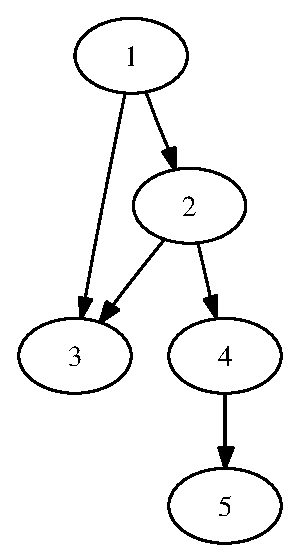
\epsfig{file=Figures/graph0,scale=0.6}
  \vspace*{-1cm}

  \caption{Ein einfacher Graph.}
  \label{fig:graph0}
\end{figure}



\noindent
In dem Graphen sind nur die unmittelbaren Verbindungen
zwischen zwei Punkten verzeichnet.  Es gibt aber unter Umst�nden auch noch
andere Verbindungen.  Beispielsweise gibt es eine unmittelbare Verbindung von
\texttt{1} nach \texttt{3}.  Es gibt dar�ber hinaus noch einen
Pfad von \texttt{1} nach \texttt{3}, der �ber den Punkt \texttt{2} geht.  
Unser Ziel in diesem Abschnitt ist es einen Algorithmus zu entwickeln, der �berpr�ft, ob
zwischen zwei Punkten eine Verbindung existiert und gegebenenfalls berechnet.
Dazu entwickeln wir zun�chst einen Algorithmus, der nur �berpr�ft, ob es eine
Verbindung zwischen zwei Punkten gibt und erweitern diesen Algorithmus dann sp�ter so, dass diese
Verbindung auch berechnet wird.

\subsection{Berechnung des transitiven Abschlusses einer Relation}
Als erstes bemerken wir, dass ein Graph $R$ nichts anderes ist als eine bin�re Relation.
Um feststellen zu k�nnen, ob es zwischen zwei Punkten eine Verbindung gibt,
m�ssen wir den transitiven Abschluss $R^+$ der Relation $R$ bilden.  Wir haben bereits
fr�her in dem Kapitel zur Mengenlehre gezeigt, dass $R^+$ wie folgt
berechnet werden kann: \\[0.2cm]
\hspace*{1.3cm} $R^+ = \bigcup\limits_{i=1}^{\infty} R^i = R \cup R^2 \cup R^3 \cup \cdots$  \\[0.2cm]
Auf den ersten Blick betrachtet sieht diese Formel so aus, als ob wir unendlich
lange rechnen m�ssten.  Aber versuchen wir einmal, diese Formel anschaulich zu
verstehen.  Zun�chst steht da $R$.  Das sind die Verbindungen, die unmittelbar  gegeben
sind.  Als n�chstes steht dort $R^2$ und das ist $R \circ R$.  Es gilt aber \\[0.2cm]
\hspace*{1.3cm} $R \circ R = \{ \pair(x,z) \mid \exists y \colon \pair(x,y) \in R \wedge \pair(y,z) \in R \}$
\\[0.2cm]
In $R^2$ sind also alle die Pfade enthalten, die aus zwei direkten Verbindungen
zusammengesetzt sind.  Allgemein l�sst sich durch Induktion sehen, dass $R^n$
alle die Pfade enth�lt, die aus $n$ direkten Verbindungen zusammengesetzt sind.  Nun
ist die Zahl der Punkte, die wir haben, endlich.  Sagen wir mal, dass es
$k$ Punkte sind.  Dann macht es  keinen Sinn solche Pfade zu betrachten, die
aus mehr als $k-1$ direkten Verbindungen zusammengesetzt sind, denn wir wollen ja
nicht im Kreis herum laufen.  Damit kann dann aber die Formel zur Berechnung des
transitiven Abschlusses vereinfacht werden:\\[0.2cm]
\hspace*{1.3cm} 
$R^+ = \bigcup\limits_{i=1}^{k-1} R^i$.
\\[0.2cm]
Diese Formel k�nnten wir tats�chlich so benutzen.  Es ist aber noch effizienter,
einen Fixpunkt-Algorithmus zu verwenden.  Dazu zeigen wir zun�chst, dass der transitive
Abschluss $R^+$ die folgende Fixpunkt-Gleichung erf�llt:
\begin{equation}
  \label{fixpunkt}
  R^+ = R \cup R \circ R^+. 
\end{equation}
Wir erinnern hier daran, dass wir vereinbart haben, dass der Operator $\circ$ st�rker
bindet als der Operator $\cup$, so dass der Ausdruck $R \cup R \circ R^+$ als
$R \cup (R \circ R^+)$ zu lesen ist.
Die Fixpunkt-Gleichung \ref{fixpunkt} l�sst sich algebraisch beweisen.  Es gilt
\[
\begin{array}{cll}
    & R \cup R \circ R^+ \\[0.2cm]
  = & R \cup R \circ \bigcup\limits_{i=1}^{\infty} R^i \\[0.4cm]
  = & R \cup R \circ \bigl(R^1 \cup R^2 \cup R^3 \cup \cdots \bigr) \\[0.2cm]
  = & R \cup \bigl(R \circ R^1 \cup R \circ R^2 \cup R \circ R^3 \cup \cdots \bigr) &
      \mbox{Distributiv-Gesetz} \\[0.2cm]
  = & R \cup \bigl(R^2 \cup R^3 \cup  R^4 \cup \cdots \bigr) & \mbox{Potenz-Gesetz} \\[0.2cm]
  = & R^1 \cup \bigl(R^2 \cup R^3 \cup  R^4 \cup \cdots \bigr) \\[0.2cm]
  = & \bigcup\limits_{i=1}^{\infty} R^i \\[0.4cm]
  = & R^+
\end{array}
\]
Die Gleichung \ref{fixpunkt} kann benutzt werden um den transitiven Abschluss iterativ zu
berechnen.  Wir definieren eine Folge $(T_n)_{n \in \mathbb{N}}$ durch Induktion folgt:
\begin{enumerate}
\item[I.A.] $n = 1$:         \hspace*{2.3cm} $T_1 := R$
\item[I.S.] $n \mapsto n+1$: \hspace*{1.6cm} $T_{n+1} := R \cup R \circ T_n$. 
\end{enumerate}
Die Relationen $T_n$ lassen sich auf die Relation $R$ zur�ckf�hren:
\begin{enumerate}
\item $T_1 = R$.
\item $T_2 = R \cup R \circ T_1 = R \cup R \circ R = R^1 \cup R^2$.
\item $\begin{array}[t]{lcl}
       T_3  & = & R \cup R \circ T_2 \\
            & = & R \cup R \circ (R^1 \cup R^2) \\
            & = & R^1 \cup R^2 \cup R^3. \\
       \end{array}
      $
\end{enumerate}
Allgemein k�nnen wir durch vollst�ndige Induktion �ber $n \in \mathbb{N}$ beweisen, dass
\[ T_n = \bigcup\limits_{i=1}^{n} R^i \]
gilt.  Der Induktions-Anfang folgt unmittelbar aus der Definition von $T_1$.  Um den 
Induktions-Schritt durchzuf�hren, betrachten wir
\[ \begin{array}{lcll}
   T_{n+1} & = & R \cup R \circ T_n & \mbox{gilt nach Definition} \\[0.2cm]
           & = & R \cup R \circ \left(\bigcup\limits_{i=1}^{n} R^i\right) &
                 \mbox{gilt nach Induktions-Voraussetzung} \\[0.4cm]
           & = & R \cup R^2 \cup \cdots \cup R^{n+1}  &
                 \mbox{Distributiv-Gesetz} \\[0.2cm]
           & = & R^1 \cup \cdots \cup R^{n+1} \\
           & = & \bigcup\limits_{i=1}^{n+1} R^i & \Box 
   \end{array}
\]
Die Folge $(T_n)_{n\in\mathbb{N}}$ hat eine weitere n�tzliche Eigenschaft: Sie ist 
\emph{monoton steigend}.  Allgemein nennen wir eine Folge von Mengen $(X_n)_{n\in\mathbb{N}}$
\emph{monoton steigend}, wenn 
\\[0.2cm]
\hspace*{1.3cm}
$\forall n \in \mathbb{N}: X_n \subseteq X_{n+1}$
\\[0.2cm]
gilt, wenn also die Mengen $X_n$ mit wachsendem Index $n$ immer gr��er werden.
Die Monotonie der Folge $(T_n)_{n \in \mathbb{N}}$ folgt aus der gerade bewiesenen Eigenschaft
$T_n = \bigcup_{i=1}^{n} R^i$, denn es gilt
\\[0.2cm]
\hspace*{1.3cm}
$
\begin{array}[t]{llcl}
                & T_n \subseteq T_{n+1} \\[0.2cm]
\Leftrightarrow & \bigcup\limits_{i=1}^{n} R^i \subseteq \bigcup\limits_{i=1}^{n+1} R^i \\[0.5cm]
\Leftrightarrow & \bigcup\limits_{i=1}^{n} R^i \subseteq \bigcup\limits_{i=1}^{n} R^i \cup R^{n+1} \\
\end{array}
$
\\[0.2cm]
und die letzte Formel ist offenbar wahr.  Ist nun die Relation $R$ endlich, so ist nat�rlich 
auch $R^+$ eine endliche Menge.  Da die 
Folge $T_n$ aber in dieser Menge liegt, denn es gilt ja 
\\[0.2cm]
\hspace*{1.3cm}
$T_n = \bigcup\limits_{i=1}^{n} R^i \subseteq \bigcup\limits_{i=1}^{\infty} R^i = R^+$ \quad f�r alle $n \in \mathbb{N}$,
\\[0.2cm]
k�nnen die Mengen $T_n$ nicht beliebig gro� werden.  Aufgrund der Monotonie der Folge
$(T_n)_{n\in\mathbb{N}}$ muss es daher einen Index $k$ geben, ab dem die Mengen $T_n$ alle gleich sind:
\\[0.2cm]
\hspace*{1.3cm}
$\forall n \in \mathbb{N}:( n \geq k \rightarrow T_n = T_k)$.
\\[0.2cm]
Ber�cksichtigen wir die Gleichung $T_n = \bigcup_{i=1}^{n} R^i$, so haben wir 
\\[0.2cm]
\hspace*{1.3cm}
$T_n = \bigcup\limits_{i=1}^{n} R^i = \bigcup\limits_{i=1}^{k} R^i = T_k$ \quad f�r alle $n \geq k$.
\\[0.2cm]
Daraus folgt dann aber, dass
\\[0.2cm]
\hspace*{1.3cm}
$T_n = \bigcup\limits_{i=1}^{n} R^i = \bigcup\limits_{i=1}^{\infty} R^i = R^+$ 
\quad f�r alle $n \geq k$  
\\[0.2cm]
gilt.  Der Algorithmus zur Berechnung von $R^+$ sieht nun so aus, dass wir die Iteration
\[ T_{n+1} := R \cup R \circ T_n \]
solange durchf�hren bis $T_{n+1} = T_n$ gilt, denn dann gilt auch $T_n = R^+$.


\begin{figure}[!ht]
  \centering
\begin{Verbatim}[ frame         = lines, 
                  framesep      = 0.3cm, 
                  labelposition = bottomline,
                  numbers       = left,
                  numbersep     = -0.2cm,
                  xleftmargin   = 0.8cm,
                  xrightmargin  = 0.8cm,
                ]
    closure := procedure(r) {
        t := r;
        while (true) {
            oldT := t;
            t    := r + product(r, t);
            if (t == oldT) {
                return t;
            }
        }
    };
    product := procedure(r1, r2) {
        return { [x,z] : [x,y] in r1, [y,z] in r2 };
    };
    r := { [1,2], [2,3], [1,3], [2,4], [4,5] };
    print( "r = ", r );
    print( "computing transitive closure of r" );
    t := closure(r);
    print( "r+ = ", t );
\end{Verbatim} 
\vspace*{-0.3cm}
\caption{Berechnung des transitiven Abschlusses.}  
\label{fig:transitive-closure.stlx}
\end{figure} %\$

\noindent
Das Programm 
\href{http://wwwlehre.dhbw-stuttgart.de/stroetmann/Logic/SetlX/transitive-closure.stlx}{\texttt{transitive-closure.stlx}}
in Abbildung
\ref{fig:transitive-closure.stlx} auf Seite \pageref{fig:transitive-closure.stlx}  zeigt
eine Implementierung dieses Gedankens.
Lassen wir dieses Programm laufen, so erhalten wir als Ausgabe:
\begin{verbatim}
    R = {[2, 3], [4, 5], [1, 3], [2, 4], [1, 2]}
    R+ = {[1, 5], [2, 3], [4, 5], [1, 4], [1, 3], [2, 4], [1, 2], [2, 5]}
\end{verbatim}
Der transitive Abschluss $R^+$ der Relation $R$ l�sst sich jetzt anschaulich
interpretieren:  Er enth�lt alle Paare $\pair(x,y)$, f�r die es einen \emph{Pfad} von
$x$ nach $y$ gibt.  Ein Pfad von $x$ nach $y$ ist dabei eine Liste der
Form \\[0.2cm]
\hspace*{1.3cm} $\bigl[ x_1, x_2, \cdots, x_n \bigr]$,
\\[0.2cm]
f�r die $x = x_1$ und $y = x_n$ gilt und f�r die au�erdem 
\\[0.2cm]
\hspace*{1.3cm}
$\pair(x_i, x_{i+1}) \in R$ \quad f�r alle $i = 1, \cdots, n-1$ gilt.
\\[0.2cm]
Die Funktion $\textsl{product}(r_1, r_2)$ berechnet das relationale Produkt $r_1 \circ
r_2$ nach der Formel
\\[0.2cm]
\hspace*{1.3cm}
$r_1 \circ r_2 = \{ \langle x, z \rangle \mid \exists y: \pair(x,y) \in r_1 \wedge \pair(y,z) \in r_2 \}$.
\\[0.2cm]
Die Implementierung dieser Prozedur  zeigt die allgemeine
Form der Mengen-Defi\-nition durch Iteratoren in \textsc{SetlX}.  Allgemein k�nnen wir eine Menge
durch den Ausdruck
\\[0.2cm]
\hspace*{1.3cm}
$\{\; \textsl{expr} \;\texttt{:}\; [x^{(1)}_1, \cdots, x^{(1)}_{n(1)}] \;\texttt{in}\; s_1,
     \cdots, [x^{(k)}_1, \cdots, x^{(k)}_{n(k)}] \;\texttt{in}\; s_k \;\texttt{|}\;
     \textsl{cond} \;\}
$
\\[0.2cm]
definieren.  Dabei muss $s_i$ f�r alle $i=1, \cdots, k$ eine Menge von Listen  der L�nge
$n(i)$ sein.  Bei der Auswertung dieses Ausdrucks werden f�r die Variablen 
$x^{(i)}_1, \cdots, x^{(i)}_{n(i)}$ die Werte eingesetzt, die die entsprechenden
Komponenten der Listen haben, die in der Menge $s_i$ auftreten.  Beispielsweise w�rde die
Auswertung von 
\begin{verbatim}
    s1 := { [ 1, 2, 3 ], [ 5, 6, 7 ] };
    s2 := { [ "a", "b" ], [ "c", "d" ] };
    m := { [ x1, x2, x3, y1, y2 ] : [ x1, x2, x3 ] in s1, [ y1, y2 ] in s2 };
\end{verbatim}
f�r \texttt{M} die Menge
\begin{verbatim}
    { [1, 2, 3, "a", "b"], [5, 6, 7, "c", "d"],  
      [1, 2, 3, "c", "d"], [5, 6, 7, "a", "b"] }
\end{verbatim}
berechnen. 


\subsection{Berechnung der Pfade}
Als n�chstes wollen wir das Programm zur Berechnung des transitiven Abschlusses so
erweitern, dass wir nicht nur feststellen k�nnen, dass es einen Pfad zwischen zwei Punkten
gibt, sondern dass wir diesen auch berechnen k�nnen.  Die Idee ist, dass wir statt des
relationalen Produkts, das f�r zwei Relationen definiert ist, ein sogenanntes
\emph{Pfad-Produkt}, das auf Mengen von Pfaden definiert ist, berechnen.  Vorab f�hren wir
f�r Pfade, die wir ja durch Listen repr�sentieren,
drei Begriffe ein.
\begin{enumerate}
\item Die Funktion $\textsl{first}(p)$ liefert den ersten Punkt der Liste $p$: \\[0.2cm]
      \hspace*{1.3cm} $\textsl{first}\bigl([x_1,\cdots,x_m]\bigr) = x_1$.
\item Die Funktion $\textsl{last}(p)$ liefert den letzten Punkt der Liste $p$: \\[0.2cm]
      \hspace*{1.3cm} $\textsl{last}\bigl([x_1,\cdots,x_m]\bigl) = x_m$.
\item Sind $p = [ x_1, \cdots, x_m ]$ und $q =[ y_1, \cdots, y_n ]$ 
      zwei Pfade mit $\textsl{first}(q) = \textsl{last}(p)$, dann definieren wir 
      die Summe von $p$ und $q$       als \\[0.2cm]
      \hspace*{1.3cm}
      $p \oplus q := [x_1, \cdots, x_m, y_2, \cdots, y_n ]$.
\end{enumerate}
Sind nun $P_1$ und $P_2$ Mengen von Pfaden, so definieren wir das  \emph{Pfad-Produkt} von
$P_1$ und $P_2$ als \\[0.2cm]
\hspace*{1.3cm} 
$P_1 \bullet P_2 := \bigl\{\; p_1 \oplus p_2 \mid p_1 \in P_1 \wedge p_2 \in P_2 \wedge \textsl{last}(p_1) = \textsl{first}(p_2) \;\bigr\}$.

\begin{figure}[!ht]
  \centering
\begin{Verbatim}[ frame         = lines, 
                  framesep      = 0.3cm, 
                  labelposition = bottomline,
                  numbers       = left,
                  numbersep     = -0.2cm,
                  xleftmargin   = 0.8cm,
                  xrightmargin  = 0.8cm,
                ]
    closure := procedure(r) {
        p := r;
        while (true) {
            oldP := p;
            p    := r + pathProduct(r, p);
            if (p == oldP) {
                return p;
            }
        }
    };
    pathProduct := procedure(p, q) {
        return { add(x, y) : x in p, y in q | x[#x] == y[1] };
    };    
    add := procedure(p, q) {
        return p + q[2..];
    };    
    r := { [1,2], [2,3], [1,3], [2,4], [4,5] };
    print( "r = ", r );
    print( "computing all paths" );
    p := closure(r);
    print( "p = ", p );
\end{Verbatim} 
\vspace*{-0.3cm}
\caption{Berechnung aller Verbindungen.}  \label{path.stlx}
\end{figure} %\$

\begin{figure}[!ht]
  \centering
  \vspace*{-9cm}

  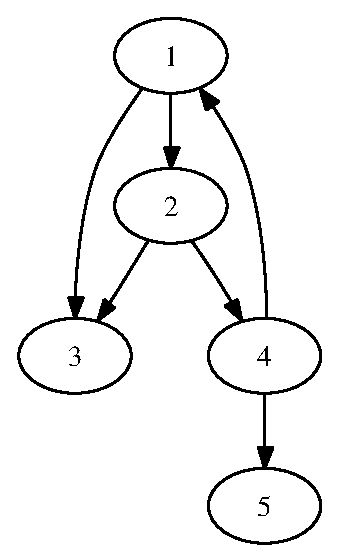
\epsfig{file=Figures/graph-zykl,scale=0.5}
  \vspace*{-1cm}

  \caption{Ein zyklischer Graph.}
  \label{fig:graph-zykl}
\end{figure}

Damit k�nnen wir das Programm in Abbildung
\ref{fig:transitive-closure.stlx} so ab�ndern, dass alle m�glichen Verbindungen zwischen zwei
Punkten berechnet werden.  Abbildung
\ref{path.stlx} zeigt das resultierende Programm
\href{http://wwwlehre.dhbw-stuttgart.de/stroetmann/Logic/SetlX/path.stlx}{\texttt{path.stlx}}. 
Leider funktioniert das Programm dann nicht mehr, wenn der Graph Zyklen enth�lt.
Abbildung
\ref{fig:graph-zykl} zeigt einen Graphen, der einen Zyklus enth�lt.  In diesem Graphen
gibt es unendlich viele Pfade, die von dem Punkt 1 zu dem Punkt 2 f�hren: \\[0.2cm]
\hspace*{1.3cm} $[ 1, 2 ]$, $[ 1, 2, 4, 1, 2 ]$, 
$[ 1, 2, 4, 1, 2, 4, 1, 2 ]$, 
$[ 1, 2, 4, 1, 2, 4, 1, 2, 4, 1, 4 ]$, $\cdots$
\\[0.2cm]
Offenbar  sind die Pfade unwichtig, die einen Punkt mehrfach enthalten und die daher
zyklisch sind.  Solche Pfade sollten wir bei der Berechnung des Pfad-Produktes
eliminieren.

\begin{figure}[!ht]
  \centering
\begin{Verbatim}[ numbers       = left,
                  numbersep     = -0.2cm,
                  frame         = lines, 
                  framesep      = 0.3cm, 
                  labelposition = bottomline,
                  xleftmargin   = 0.0cm,
                  xrightmargin  = 0.0cm,
                ]
    pathProduct := procedure(p, q) {
        return { add(x,y) : x in p, y in q | x[#x] == y[1] && noCycle(x,y) };
    };
    noCycle := procedure(l1, l2) {
        return #({ x : x in l1 } * { x : x in l2 }) == 1;
    };
\end{Verbatim} 
\vspace*{-0.3cm}
\caption{Berechnung aller Verbindungen in zyklischen Graphen}  
\label{fig:path-cyclic.stlx}
\end{figure} %\$

Abbildung \ref{fig:path-cyclic.stlx} zeigt einen Ausschnitt des ge�nderten Programms
\href{http://wwwlehre.dhbw-stuttgart.de/stroetmann/Logic/SetlX/path-cyclic.stlx}{\texttt{path-cyclic.stlx}},
das auch f�r zyklische Graphen funktioniert. 
\begin{enumerate}
\item In Zeile 2 ber�cksichtigen wir nur die Pfade $x \oplus y$, die nicht zyklisch sind.
\item In Zeile 5 �berpr�fen wir, ob die Konkatenation  $l_1 \oplus l_2$ zyklisch ist.  Die
      Kombination von $l_1$ und $l_2$  ist genau dann 
      zyklisch, wenn die Listen $l_1$ und $l_2$ mehr als ein gemeinsames Element
      enthalten.  Die Listen $l_1$ und $l_2$ enthalten mindestens ein gemeinsames Element,
      denn wir verkn�pfen diese beiden Listen ja nur dann, wenn das letzte Element
      der Liste $l_1$ mit dem ersten Element der Liste $l_2$ �bereinstimmt.
      Wenn es nun noch einen weiteren Punkt geben w�rde, der sowohl in $l_1$ als auch in
      $l_2$ auftreten w�rde, dann w�re der Pfad $l_1 \oplus l_2$ zyklisch.
\end{enumerate}

In den meisten F�llen sind wird gar nicht daran interessiert, alle m�glichen Verbindungen
zwischen allen Punkten zu berechnen, das w�re n�mlich viel zu aufwendig, sondern wir
wollen nur zwischen zwei gegebenen Punkten 
eine Verbindung finden.  Abbildung \ref{fig:find-path} zeigt die Implementierung einer
Prozedur $\texttt{reachable}(x, y, r)$, die �berpr�ft, ob es in dem Graphen $r$ eine
Verbindung von $x$ nach $y$ gibt und die diese Verbindung berechnet.  Das vollst�ndige
Programm finden Sie in der Datei
\href{http://wwwlehre.dhbw-stuttgart.de/stroetmann/Logic/SetlX/find-path.stlx}{\texttt{find-path.stlx}}.
Wir diskutieren nun die Implementierung der Prozedur \texttt{reachable}.
\begin{enumerate}
\item In Zeile 2 initialisieren wir $p$ so, dass zun�chst nur der Pfad der L�nge 0,
      der mit dem Punkt $x$  startet, in $p$ liegt.
\item In Zeile 6 selektieren wir die Pfade aus $p$, die zum Ziel $y$ f�hren.
\item Wenn wir dann in Zeile 7 feststellen, dass wir einen solchen Pfad berechnet haben,
      geben wir einen dieser Pfade in Zeile 8 zur�ck.
\item Falls es nicht gelingt einen solchen Pfad zu berechnen und wir keine neuen
      Pfade mehr finden k�nnen, verlassen wir die Prozedur in Zeile 11
      mit dem Befehl \texttt{return}.  Da wir bei diesem \texttt{return}-Befehl
      keinen Wert zur�ckgeben, ist der R�ckgabewert der Prozedur in diesem Fall
      automatisch $\Omega$.
\end{enumerate}

\begin{figure}[!ht]
  \centering
\begin{Verbatim}[ frame         = lines, 
                  framesep      = 0.3cm, 
                  labelposition = bottomline,
                  numbers       = left,
                  numbersep     = -0.2cm,
                  xleftmargin   = 0.8cm,
                  xrightmargin  = 0.8cm,
                ]
    reachable := procedure(x, y, r) {
        p := { [x] };
        while (true) {
            oldP  := p;
            p     := p + pathProduct(p, r);
            found := { l in p | l[#l] == y };
            if (found != {}) {
                return arb(found);
            }
            if (p == oldP) {
                return;
            }
        }
    };
\end{Verbatim} 
\vspace*{-0.3cm}
\caption{Berechnung aller Verbindungen zwischen zwei Punkten}  
\label{fig:find-path}
\end{figure} %\$

\subsection{Der Bauer mit dem Wolf, der Ziege und dem Kohl}
Wir pr�sentieren nun eine betriebswissenschaftliche Anwendung des oben entwickelten Algorithmus und
betrachten folgendes Problem.
\vspace*{0.3cm}

\begin{minipage}[c]{14cm}
{\sl
Ein Agrar�konom will mit einem Wolf, einer Ziege und einem Kohl �ber einen Fluss �bersetzen, um
diese als Waren auf dem Markt zu verkaufen.
Das Boot ist aber so klein, dass er nicht mehr als zwei Waren gleichzeitig mitnehmen kann.
Wenn der Bauer den Wolf mit der Ziege allein l�sst, dann frisst der Wolf die Ziege und wenn er die
Ziege mit dem Kohl allein l�sst, dann frisst die Ziege den Kohl. }
\end{minipage}
\vspace*{0.3cm}

\noindent
Wir wollen einen Fahrplan entwickeln, mit dem der Agrar�konom alle seine Waren unbeschadet zum
Markt bringen kann.  Dazu modellieren wir das R�tsel als Erreichbarkeits-Problem in einem
Graphen.  
Die Punkte des Graphen beschreiben dabei die einzelnen Situationen, die auftreten
k�nnen.  Wir definieren eine Menge\\[0.2cm]
\hspace*{1.3cm} 
$\texttt{all} := \{ \squote{Bauer}, \squote{Wolf}, \squote{Ziege},\squote{Kohl} \}$.
\\[0.2cm]
Die einzelnen Punkte sind dann Paare von Mengen, haben also die Form \\[0.2cm]
\hspace*{1.3cm} 
$\langle s_1, s_2 \rangle$ \quad mit $s_1,s_2 \subseteq \texttt{all}$.
\\[0.2cm]
Dabei gibt die Menge $s_1$ an, was am linken Ufer ist und $s_2$ gibt an, was am rechten
Ufer ist.  Die Menge aller Punkte k�nnen wir dann definieren als \\[0.2cm]
\hspace*{1.3cm} 
$p := \bigl\{ \langle s_1, s_2 \rangle \in 2^\texttt{all} \times 2^\texttt{all} \;|\;
              s_1 \cup s_2 = \texttt{all} \;\wedge\; s_1 \cap s_2 = \{\} 
      \bigr\}
$.
\\[0.2cm]
Die Bedingung $s_1 \cup s_2 = \texttt{all}$ stellt dabei sicher, dass nichts verloren
geht:  Jedes der Elemente aus \texttt{all} ist entweder am linken oder am rechten Ufer.
Die Bedingung $s_1 \cap s_2 = \{\}$ verbietet die Bilokalisation von Objekten, sie stellt also sicher,
dass kein Element aus der Menge \texttt{all}  gleichzeitig am  linken und am rechten Ufer ist.

Als n�chstes definieren wir den Graphen $r$, also die m�glichen Verbindungen zwischen
Punkten.  Dazu definieren wir eine Prozedur $\textsl{problem}(s)$. Hierbei ist $s$ eine
Menge von Objekten, die an einem Ufer sind.  Die Prozedur $\textsl{problem}(s)$
liefert genau dann \texttt{true}, wenn es bei der  Menge $s$ ein Problem gibt, weil entweder die Ziege
mit dem Kohl allein ist, oder aber der Wolf die Ziege frisst.
\begin{verbatim}
    problem := procedure(s) {
        return "goat" in s && "cabbage" in s || "wolf" in s && "goat" in s;
    };
\end{verbatim}
Damit k�nnen wir eine Relation $r_1$ wie folgt definieren:
\\[0.2cm]
\hspace*{1.3cm} 
$r_1 := \Bigl\{ \bigl\langle \pair(s_1, s_2), \pair(s_1 \backslash b, s_2 \cup b)
  \bigr\rangle \;|\; $ \\
\hspace*{2.3cm} 
$\pair(s_1, s_2) \in P \;\wedge\; b \subseteq s_1 \;\wedge\;
 \squote{Bauer} \in b \;\wedge\; \textsl{card}(b) \leq 2 \;\wedge\; \neg\textsl{problem}(s_1 \backslash b) \Bigr\}$.
\\[0.2cm]
Diese Menge beschreibt alle die Fahrten, bei denen der Bauer vom linken Ufer zum rechten Ufer
f�hrt und bei denen zus�tzlich sichergestellt ist, dass am linken Ufer
nach der �berfahrt kein Problem auftritt.  Die einzelnen Terme werden wie folgt
interpretiert:
\begin{enumerate}
\item $\pair(s_1,s_2)$ ist der Zustand vor der �berfahrt des Bootes,
      $s_1$ gibt also die Objekte am linken Ufer an, $s_2$ sind die Objekte am rechten Ufer.
\item $b$ ist der Inhalt des Bootes, daher beschreibt 
       $\pair(s_1 \backslash b, s_2 \cup b)$ den Zustand nach der �berfahrt des Bootes:
       Links sind nun nur noch die Objekte aus $s_1 \backslash b$, daf�r sind rechts dann 
       die Objekte $s_2 \cup b$.

       Die Bedingungen lassen sich wie folgt interpretieren.
\item $b \subseteq s_1$: Es k�nnen nat�rlich nur solche Objekte ins Boot genommen werden,
       die vorher am linken Ufer waren.
\item $\squote{Bauer} \in b$: Der Bauer muss auf jeden Fall ins Boot, denn weder der Wolf
       noch die Ziege k�nnen rudern.
\item $\textsl{card}(b) \leq 2$: Die Menge der Objekte im Boot darf nicht mehr als zwei
       Elemente haben, denn im Boot ist nur f�r zwei Platz.
\item $\neg\textsl{problem}(s_1 \backslash b)$:  Am linken Ufer soll es nach der �berfahrt
       kein Problem geben, denn der Bauer ist ja hinterher am rechten Ufer.
\end{enumerate}
In analoger Weise definieren wir nun eine Relation $r_2$ die die �berfahrten vom rechten
Ufer zum linken Ufer beschreibt:\\[0.2cm]
\hspace*{1.3cm} 
$r_2 := \Bigl\{ \bigl\langle \pair(s_1, s_2), \pair(s_1 \cup b, s_2 \backslash b)
  \bigr\rangle \;|\; $ \\
\hspace*{2.3cm} 
$\pair(s_1, s_2) \in P \;\wedge\; b \subseteq s_2 \;\wedge\;
 \squote{Bauer} \in b \;\wedge\; \textsl{card}(b) \leq 2 \;\wedge\; \neg\textsl{problem}(s_2 \backslash b) \Bigr\}$.
\\[0.2cm]
Die gesamte Relation $r$ definieren wir nun als
\\[0.2cm]
\hspace*{1.3cm} $r := r_1 \cup r_2$.\\[0.2cm]
Als n�chstes m�ssen wir den Start-Zustand modellieren.
Am Anfang sind alle am linken Ufer, also wird der Start-Zustand durch das Paar 
\\[0.3cm]
\hspace*{1.3cm}
$\bigl\langle \{ \squote{Bauer}, \squote{Wolf}, \squote{Ziege},\squote{Kohl} \}, \{\} \bigr\rangle$.
\\[0.3cm]
Beim Ziel ist es genau umgekehrt, dann sollen alle auf der rechten Seite des Ufers sein:
\\[0.3cm]
\hspace*{1.3cm}
$\bigl\langle \{\}, \{ \squote{Bauer}, \squote{Wolf}, \squote{Ziege},\squote{Kohl} \} \bigr\rangle$.
\\[0.3cm]
Damit haben wir das Problem in der Mengenlehre modelliert und k�nnen die im letzten
Abschnitt entwickelte Prozedur \texttt{reachable} benutzen, um das Problem zu l�sen.
In der Abbildung \ref{fig:wolf-ziege} finden Sie das Programm 
\href{http://wwwlehre.dhbw-stuttgart.de/stroetmann/Logic/SetlX/wolf-goat-cabbage.stlx}{\texttt{wolf-goat-cabbage.stlx}},
in dem die oben ausgef�hrten �berlegungen in \textsc{SetlX} umgesetzt wurden.
Die von diesem Programm berechnete L�sung finden Sie in Abbildung \ref{fig:wolf-ziege-solution}.

\begin{figure}[!ht]
  \centering
\begin{Verbatim}[ codes         = {\catcode`$=3\catcode`_=8\catcode`^=7},
                  frame         = lines, 
                  framesep      = 0.3cm, 
                  labelposition = bottomline,
                  numbers       = left,
                  numbersep     = -0.2cm,
                  xleftmargin   = 0.0cm,
                  xrightmargin  = 0.0cm,
                ]
    all := { "farmer", "wolf", "goat", "cabbage" };
    p   := pow(all);
    r1  := { [ s, s - b ] : s in p, b in pow(s) 
                          | "farmer" in b && #b <= 2 && !problem(s - b) 
           };
    r2  := { [ s, s + b ] : s in p, b in pow(all - s) 
                          | "farmer" in b && #b <= 2 && !problem(all - (s + b))
           };
    r   := r1 + r2;
    start := [ all, {} ];
    goal  := [ {}, all ];
    path := findPath(start, goal, r);
\end{Verbatim} 
\vspace*{-0.3cm}
\caption{Wie kommt der Bauer ans andere Ufer?}  
\label{fig:wolf-ziege}
\end{figure} %\$
\noindent

\begin{figure}[!ht]
  \centering
\begin{Verbatim}[ codes         = {\catcode`$=3\catcode`_=8\catcode`^=7},
                  frame         = lines, 
                  framesep      = 0.3cm, 
                  labelposition = bottomline,
                  numbers       = left,
                  numbersep     = -0.2cm,
                  commandchars  = \\\{\},
                  xleftmargin   = 0.0cm,
                  xrightmargin  = 0.0cm,
                ]
    \{"Kohl", "Ziege", "Wolf", "Bauer"\}                                        \{\}
                              >> \{"Ziege", "Bauer"\} >>
    \{"Kohl", "Wolf"\}                                          \{"Ziege", "Bauer"\}
                              << \{"Bauer"\} <<<< 
    \{"Kohl", "Wolf", "Bauer"\}                                          \{"Ziege"\}
                              >> \{"Wolf", "Bauer"\} >>>
    \{"Kohl"\}                                          \{"Ziege", "Wolf", "Bauer"\}
                              << \{"Ziege", "Bauer"\} <<
    \{"Kohl", "Ziege", "Bauer"\}                                          \{"Wolf"\}
                              >> \{"Kohl", "Bauer"\} >>>
    \{"Ziege"\}                                          \{"Kohl", "Wolf", "Bauer"\}
                              << \{"Bauer"\} <<<< 
    \{"Ziege", "Bauer"\}                                          \{"Kohl", "Wolf"\}
                              >> \{"Ziege", "Bauer"\} >>    
    \{\}                                        \{"Kohl", "Ziege", "Wolf", "Bauer"\}
\end{Verbatim} 
\vspace*{-0.3cm}
\caption{Ein Fahrplan f�r den Bauern}  
\label{fig:wolf-ziege-solution}
\end{figure} %$
\pagebreak

\vspace*{\fill}
\pagebreak

\section{Terme und Matching}
Neben den bisher vorgestellten Datenstrukturen gibt es noch eine weitere wichtige
Datenstruktur, die sogenannten \emph{Terme}, die insbesondere n�tzlich ist, wenn wir
\emph{symbolische Programme} 
schreiben wollen.  Darunter verstehen wir solche Programme, die Formeln manipulieren.
Wollen wir beispielsweise ein Programm schreiben, dass als Eingabe einen String wie
\\[0.2cm]
\hspace*{1.3cm}
``\texttt{x * sin(x)}''
\\[0.2cm]
einliest, diesen String als eine Funktion in der Variablen ``\texttt{x}'' interpretiert
und dann die Ableitung dieser Funktion nach der Variablen ``\texttt{x}'' berechnet, so
sprechen wir von einem \emph{symbolischen Programm}.   Wollen wir einen Ausdruck wie 
``\texttt{x * sin(x)}'' darstellen, so eignen sich \emph{Terme} am besten dazu.
Im n�chsten Unter-Abschnitt werden wir zun�chst \emph{Terme} zusammen mit den in \setl\
vordefinierten Funktionen vorstellen, die zur Verarbeitung von Termen benutzt werden k�nnen.
Anschlie�end stellen wir das sogenannte \emph{Matching} vor, mit dessen Hilfe sich Terme
besonders leicht manipulieren lassen.


\subsection{Konstruktion und Manipulation von Termen}
Terme werden mit Hilfe sogenannter \emph{Funktions-Zeichen} gebildet.  Es ist wichtig,
dass Sie Funktions-Zeichen nicht mit Funktionen oder Variablen verwechseln.  In \setl\
beginnen Funktionen-Zeichen im Gegensatz zu einem Variablen-Namen daher mit einem gro�en
Buchstaben.  Auf den Gro�buchstaben k�nnen  dann beliebig viele Buchstaben, Ziffern und
der Unterstrich ``\texttt{\_}'' folgen.
Zus�tzlich gibt es noch Funktionszeichen, die mit dem Zeichen
``\texttt{\symbol{94}}''
beginnen.  Solche Funktions-Zeichen werden intern von \setl\ verwendet um Operator-Symbole
wie ``\texttt{+}'' oder ``\texttt{*}'' darzustellen.
Die folgenden Strings k�nnen beispielsweise  als Funktions-Zeichen vewendet werden:
\\[0.2cm]
\hspace*{1.3cm}
\texttt{F}, \quad \texttt{FabcXYZ}, \quad \texttt{\symbol{94}sum}, \quad \texttt{Hugo\_}.
\\[0.2cm]
Damit sind wir nun in der Lage, Term zu definieren.  Ist $F$ ein Funktions-Zeichen und sind
$t_1$, $t_2$, $\cdots$, beliebige \setl-Werte, so ist der Ausdruck
\\[0.2cm]
\hspace*{1.3cm}
$F(t_1, t_2, \cdots, t_n)$
\\[0.2cm]
ein Term.  Beachten Sie, dass Terme ganz �hnlich aussehen wie die Aufrufe von Funktionen.
Terme und Aufrufe von Funktionen unterscheiden sich nur dadurch, dass bei einem Term links
vor der ersten �ffnenden Klammer ein Funktions-Zeichen steht, w�hrend bei einem
Funktions-Aufruf dort statt dessen eine Variable steht, der eine Funktions-Definition zugewiesen
worden ist.

\examples
\begin{enumerate}
\item \texttt{Adresse(\symbol{34}Roteb�hlplatz 41\symbol{34}, 70178, \symbol{34}Stuttgart\symbol{34})}

      ist ein Term, der eine Adresse repr�sentiert.
\item \texttt{Product(Variable(\symbol{34}x\symbol{34}), Sin(Variable(\symbol{34}x\symbol{34})))}

      ist ein Term, der einen arithmetischen Ausdruck repr�sentiert, den Sie mathematisch
      als $x * \sin(x)$ schreiben w�rden.  \eox
\end{enumerate}

An dieser Stelle fragen Sie sich vielleicht, wie Terme ausgewertet werden.  Die Antwort ist:
\textbf{Gar nicht!}  Terme werden nur dazu benutzt, Daten darzustellen.  Terme sind also bereits 
Werte  genauso wie auch Zahlen, Strings, Mengen oder Listen als Werte aufgefasst werden.
Genausowenig wie Sie die Zahl \texttt{42} auswerten m�ssen, m�ssen Sie einen Term auswerten.

Nehmen wir einmal an,
dass es in \setl\ keine Listen geben w�rde.  Dann k�nnten wir Listen als Terme darstellen.  Zun�chst
w�rden wir ein Funktions-Zeichen ben�tigen, mit dem wir die leere Liste darstellen k�nnten.  Wir
w�hlen dazu das Funktions-Zeichen \texttt{Nil}.  Damit haben wir dann also die Entsprechung
\\[0.2cm]
\hspace*{1.3cm}
$\texttt{Nil}() \;\widehat{=}\; \texttt{[]}$.
\\[0.2cm]
\textbf{Beachten} Sie hier, dass die Klammern hinter dem Funktions-Zeichen \texttt{Nil} nicht
weggelassen werden d�rfen!  Um nun eine Liste darzustellen, deren erstes Element $x$ ist und deren
restliche Elemente durch die Restliste $r$ gegeben sind, verwenden wir das Funktions-Zeichen
\texttt{Cons}.  Dann haben wir die Entsprechung
\\[0.2cm]
\hspace*{1.3cm}
$\texttt{Cons(x, r)} \;\widehat{=}\; \texttt{[}x\texttt{]}+r$. 
\\[0.2cm]
Konkret k�nnen wir nun die Liste \texttt{[1,2,3]} durch den Term
\\[0.2cm]
\hspace*{1.3cm}
\texttt{Cons(1, Cons(2, Cons(3, Nil())))}
\\[0.2cm]
darstellen.  In der Sprache \textsl{Prolog}, die wir sp�ter noch besprechen werden, werden Listen
intern �brigens in �hnlicher Form als Terme dargestellt.

Es gibt zwei vordefinierte Funktionen in \setl, mit denen wir auf die Komponenten eines Terms
zugreifen k�nnen und es gibt eine Funktion, mit deren Hilfe wir Terme konstruieren k�nnen.
\begin{enumerate}
\item Die Funktion \texttt{fct} berechnet das Funktions-Zeichen eines Terms.
      Falls $t$ ein Term der Form $F(s_1,\cdots,s_n)$ ist, so ist das Ergebnis des Funktions-Aufrufs
      \\[0.2cm]
      \hspace*{1.3cm}
      $\texttt{fct}(F(s_1,\cdots,s_n))$
      \\[0.2cm]
      das Funktions-Zeichen $F$ dieses Terms.  Beispielsweise liefert der Ausdruck
      \\[0.2cm]
      \hspace*{1.3cm}
      \texttt{fct(Cons(1, Cons(2, Cons(3, Nil()))))}
      \\[0.2cm]
      als Ergebnis das Funktions-Zeichen \texttt{\symbol{34}Cons\symbol{34}}.
\item Die Funktion \texttt{args} berechnet die Argumente eines Terms.
      Falls $t$ ein Term der Form $F(s_1,\cdots,s_n)$ ist, dann liefert der Ausdruck
      \\[0.2cm]
      \hspace*{1.3cm}
      $\mathtt{args}(F(s_1,\cdots,s_n))$
      \\[0.2cm]
      als Ergebnis die Liste $[s_1, \cdots, s_n]$ der Argumente des Terms $t$  .  Beispielsweise
      liefert der Ausdruck
      \\[0.2cm]
      \hspace*{1.3cm}
      \texttt{args(Cons(1, Cons(2, Cons(3, Nil()))))}
      \\[0.2cm]
      das Ergebnis
      \\[0.2cm]
      \hspace*{1.3cm}
      \texttt{[1, Cons(2, Cons(3, Nil()))]}.
\item Ist ein Funktions-Zeichen $f$ und eine Liste $l$ von Argumenten gegeben, so erzeugt die
      Funktion \texttt{makeTerm} durch den Aufruf
      \\[0.2cm]
      \hspace*{1.3cm}
      $\texttt{makeTerm}(f,l)$
      \\[0.2cm]
      einen Term $t$ mit dem Funktions-Zeichen $f$ und der Argument-Liste $l$, f�r $t$ gilt also
      \\[0.2cm]
      \hspace*{1.3cm}
      $\mathtt{fct}(t) = f$  \quad und \quad $\mathtt{args}(t) = l$.
      \\[0.2cm]
      Beispielsweise liefert der Aufruf
      \\[0.2cm]
      \hspace*{1.3cm}
      \texttt{makeTerm(\symbol{34}Cons\symbol{34}, [ 1, Nil() ])}
      \\[0.2cm]
      als Ergebnis den Term
      \\[0.2cm]
      \hspace*{1.3cm}
      \texttt{Cons(1,Nil())}.
      \\[0.2cm]
      Diesen Term h�tten wir nat�rlich auch unmittelbar hinschreiben k�nnen.
\end{enumerate}

\begin{figure}[!ht]
\centering
\begin{Verbatim}[ frame         = lines, 
                  framesep      = 0.3cm, 
                  firstnumber   = 1,
                  labelposition = bottomline,
                  numbers       = left,
                  numbersep     = -0.2cm,
                  xleftmargin   = 0.8cm,
                  xrightmargin  = 0.8cm,
                ]
    append := procedure(l, x) {
        if (fct(l) == "Nil") {
            return Cons(x, Nil());
        }
        [head, tail] := args(l);
        return Cons(head, append(tail, x));
    };
\end{Verbatim}
\vspace*{-0.3cm}
\caption{Einf�gen eines Elements am Ende einer Liste.}
\label{fig:append.stlx}
\end{figure}

In Abbildung  \ref{fig:append.stlx} auf Seite \pageref{fig:append.stlx} sehen Sie die
Implementierung  einer Funktion
\href{http://wwwlehre.dhbw-stuttgart.de/stroetmann/Logic/SetlX/append.stlx}{\texttt{append}},
deren Aufgabe es ist, ein Element $x$ am Ende einer Liste $l$ einzuf�gen, wobei vorausgesetzt ist,
dass die Liste $l$ als Term mit Hilfe der Funktions-Zeichen ``\texttt{Cons}'' und ``\texttt{Nil}''
dargestellt wird.
\begin{enumerate}
\item Zun�chst wird in Zeile 2 �berpr�ft, ob die Liste $l$ leer ist.  Die Liste $l$ ist genau dann
      leer, wenn $l = \texttt{Nil()}$ gilt.  Daher k�nnen wir einfach das Funktions-Zeichen von dem
      Term $l$ testen um herauszufinden, ob $l$ die leere Liste repr�sentiert.
\item Falls $l$ nicht leer ist, muss $l$ die Form
      \\[0.2cm]
      \hspace*{1.3cm}
      $l = \texttt{Cons(\textsl{head}, \textsl{tail})}$
      \\[0.2cm]     
      haben.  Dann ist \textsl{head} das erste Element der Liste $l$ und \textsl{tail} bezeichnet
      die Liste der restlichen Elemente.  In diesem Fall m�ssen wir $x$ rekursiv in die Liste
      \textsl{tail} einf�gen.  Als Ergebnis wird in Zeile 6 dann eine neue Liste erzeugt, deren
      erstes Element \textsl{head} ist, w�hrend die Liste der restlichen Elemente durch den
      rekursiven Aufruf von \textsl{append} berechnet wird.
\end{enumerate}
In manchen F�llen ist es sehr unbequem, dass Funktions-Zeichen immer mit einem gro�en Buchstaben
beginnen m�ssen.  Deswegen gibt es in \setl\ einen Escape-Mechanismus, der es erlaubt, auch
Funktionszeichen zu verwenden, die mit einem kleinen Buchstaben beginnen:  Falls wir einem
Funktionszeichen den Operator ``\texttt{\symbol{64}}'' voranstellen, dann darf das Funktionszeichen
auch mit einem kleinen Buchstaben beginnen.  Wollen wir beispielsweise Terme benutzen um
algebraische Ausdr�cke darzustellen, die trigonometrische Funktionen enthalten, 
so k�nnen wir einen Ausdruck der Form $\sin(x)$ durch den Term
\\[0.2cm]
\hspace*{1.3cm}
\texttt{\symbol{64}sin(\symbol{34}x\symbol{34})}  
\\[0.2cm]
darstellen.

\subsection{Matching}
Der Umgang mit Termen w�re sehr m�hsam, wenn wir die Terme jedesmal mit Hilfe der Funktionen
\texttt{fct} und \texttt{args} auseinander nehmen m�ssten.  Abbildung \ref{fig:append-match.stlx} 
zeigt eine weitere Implementierung der Funktion
\href{http://wwwlehre.dhbw-stuttgart.de/stroetmann/Logic/SetlX/append-match.stlx}{\texttt{append}}, 
bei der wir die Kontroll-Struktur \texttt{match} an Stelle der Funktionen ``\texttt{fct}''
and ``\texttt{args}'' verwendet haben.  In Zeile 3 wird  �berpr�ft, ob die Liste $l$ leer ist.
Die wahre St�rke des Matchings sehen wir allerdings ist in Zeile 4, denn dort wird nicht nur
�berpr�ft, ob die Liste $l$ die Form
\\[0.2cm]
\hspace*{1.3cm}
\texttt{Cons(\textsl{head},\textsl{tail})}
\\[0.2cm]
hat, sondern gleichzeitig werden die Variablen \textsl{head} and \textsl{tail} so gesetzt, dass
anschlie�end die Gleichung
\\[0.2cm]
\hspace*{1.3cm}
$l = \texttt{Cons(\textsl{head},\textsl{tail})}$
\\[0.2cm]
erf�llt ist.


\begin{figure}[!ht]
\centering
\begin{Verbatim}[ frame         = lines, 
                  framesep      = 0.3cm, 
                  firstnumber   = 1,
                  labelposition = bottomline,
                  numbers       = left,
                  numbersep     = -0.2cm,
                  xleftmargin   = 0.8cm,
                  xrightmargin  = 0.8cm,
                ]
    append := procedure(l, x) {
        match (l) {
            case Nil():            return Cons(x, Nil());
            case Cons(head, tail): return Cons(head, append(tail, x));
        }
    };
\end{Verbatim}
\vspace*{-0.3cm}
\caption{Implementierung von \texttt{append} mit Hilfe von \emph{Matching}.}
\label{fig:append-match.stlx}
\end{figure}

Im Allgemeinen ist  ein \texttt{match}-Block so �hnlich aufgebaut wie ein
\texttt{switch}-Block und hat die in Abbildung \ref{fig:match} gezeigte Struktur.
Hier bezeichnet $e$ einen Ausdruck, dessen Auswertung einen Term ergibt.  
Die Ausdr�cke $t_1$, $\cdots$, $t_n$ sind sogenannte \emph{Muster}, die freie
Variablen enthalten.  Bei der Auswertung eines \texttt{Match}-Blocks versucht
\textsc{SetlX} die in dem Muster $t_i$ auftretenden Variablen so zu setzen, dass das Muster
zu dem Ergebnis der Auswertung von $e$ gleich ist.  Gelingt dies, so wird die
mit $\textsl{body}_i$ bezeichnete Gruppe von Befehlen ausgef�hrt.  Andernfalls
versucht \textsc{SetlX} das n�chste Muster $t_{i+1}$ mit $e$ zur Deckung zu bringen.
Falls keines der Muster $t_1$, $\cdots$, $t_n$ mit $e$ zur Deckung zu bringen ist, wird
ersatzweise $\textsl{body}_{n+1}$ ausgef�hrt.  

\begin{figure}[!ht]
  \centering
\begin{Verbatim}[ codes         = {\catcode`_=8\catcode`^=7},
                  frame         = lines, 
                  framesep      = 0.3cm, 
                  labelposition = bottomline,
                  numbers       = left,
                  numbersep     = -0.2cm,
                  commandchars  = \\\{\},
                  xleftmargin   = 0.8cm,
                  xrightmargin  = 0.8cm
                ]
      \texttt{\underline{match} (\(e\)) \{}
          \texttt{\underline{case}} \(t_1\) : \textsl{body}\(_1\) 
          \vdots
          \texttt{\underline{case}} \(t_n\) : \textsl{body}\(_n\)
          \texttt{\underline{default}:} \textsl{body}\(_{n+1}\)
      \texttt{\}}
\end{Verbatim}
\vspace*{-0.3cm}
\caption{Struktur eines \texttt{Match}-Blocks}  \label{fig:match}
\end{figure} 


\begin{figure}[!ht]
\centering
\begin{Verbatim}[ frame         = lines, 
                  framesep      = 0.3cm, 
                  firstnumber   = 1,
                  labelposition = bottomline,
                  numbers       = left,
                  numbersep     = -0.2cm,
                  xleftmargin   = 0.8cm,
                  xrightmargin  = 0.8cm,
                ]
    diff := procedure(t, x) {
        match (t) {
            case t1 + t2 :
                return diff(t1, x) + diff(t2, x);
            case t1 - t2 :
                return diff(t1, x) - diff(t2, x);
            case t1 * t2 :
                return diff(t1, x) * t2 + t1 * diff(t2, x);
            case t1 / t2 :
                return ( diff(t1, x) * t2 - t1 * diff(t2, x) ) / t2 * t2;
            case f ** g :
                return diff( @exp(g * @ln(f)), x);
            case ln(a) :
                return diff(a, x) / a;
            case exp(a) :
                return diff(a, x) * @exp(a);
            case ^variable(x) : // x is defined above as second argument
                return 1;
            case ^variable(y) : // y not yet defined, matches any other variable
                return 0;
            case n | isNumber(n):   
                return 0;  
        }
    };
\end{Verbatim}
\vspace*{-0.3cm}
\caption{A function to perform symbolic differentiation.}
\label{fig:diff.stlx}
\end{figure}

\noindent
Wir zeigen zum Abschluss dieses Abschnitts ein komplexeres Beispiel.  Die in Abbildung
\ref{fig:diff.stlx} auf Seite \pageref{fig:diff.stlx} gezeigte Funktion
\href{http://wwwlehre.dhbw-stuttgart.de/stroetmann/Logic/SetlX/diff.stlx}{\texttt{diff}}
wird mit zwei Argumenten aufgerufen:
\begin{enumerate}
\item Das erste  Argument $t$ ist ein Term, der einen arithmetischen Ausdruck repr�sentiert.
\item Das zweite Argument $x$ ist ein String, der als Variable interpretiert wird.
\end{enumerate}
Die Aufgabe der Funktion \texttt{diff} besteht darin, den durch $t$ gegebenen Ausdruck nach der
in $x$ angegebenen Variablen zu differenzieren.  Wollen wir beispielsweise die Funktion
\\[0.2cm]
\hspace*{1.3cm}
$x \mapsto x^x$
\\[0.2cm]
nach $x$ ableiten, so k�nnen wir die Funktion \texttt{diff} wie folgt aufrufen.
\\[0.2cm]
\hspace*{1.3cm}
\texttt{diff(parse(\symbol{34}x ** x\symbol{34}), \symbol{34}x\symbol{34});}
\\[0.2cm]
Hier wandelt die Funktion \texttt{parse} den String ``\texttt{x ** x}'' in einen Term um.  Die
genaue Struktur dieses Terms diskutieren wir weiter unten.  Wir betrachten
zun�chst den \texttt{match}-Befehl in  Abbildung \ref{fig:diff.stlx}.  
In Zeile  3 hat der zu differenzierende Ausdruck die Form
\texttt{t1 + t2}.  Um einen solchen Ausdruck nach einer Variablen $x$ zu differenzieren, m�ssen wir
sowohl  \texttt{t1} als auch \texttt{t2} nach $x$ differenzieren.  Die dabei erhaltenen Ergebnisse
sind dann zu addieren.  Etwas interessanter ist Zeile 8, welche die Produkt-Regel der
Differenzial-Rechnung umsetzt.  Die Produkt-Regel lautet:
\\[0.2cm]
\hspace*{1.3cm}
$\displaystyle \frac{d\;}{dx} \bigl(t_1 \cdot t_2\bigr) = \frac{d\, t_1}{dx} \cdot t_2 + t_1 \cdot \frac{d\,t_2}{dx}$.
\\[0.2cm]
Bemerken Sie, dass in Zeile 7 das Muster
\\[0.2cm]
\hspace*{1.3cm}
\texttt{t1 * t2}
\\[0.2cm]
zum einen dazu dient, zu erkennen, dass der zu differenzierende Ausdruck ein Produkt ist, zum
anderen aber auch die beiden Faktoren des Produkts extrahiert und an die Variablen $t_1$ und $t_2$ bindet.
In den Zeilen  12 und 16 haben wir den Funktions-Zeichen ``\texttt{exp}'' und ``\texttt{ln}'' den
 Operator ``\texttt{\symbol{64}}'' vorangestellen m�ssen, denn sonst w�rden die Strings
 ``\texttt{exp}'' und ``\texttt{ln}'' nicht als Funktions-Zeichen sondern als Variablen
 aufgefasst werden. 

Die Regel zur Berechnung der  Ableitung eines Ausdrucks der Form $f^g$ beruht auf der
Gleichung
\\[0.2cm]
\hspace*{1.3cm}
$f^g = \exp\bigl(\ln\bigl(f^g\bigr)\bigr) = \exp\bigl(g \cdot \ln(f)\bigr)$,
\\[0.2cm]
die in Zeile 12 umgesetzt wird.  

Um einen Ausdruck der Form $\ln(f)$ abzuleiten, m�ssen
wir die Kettenregel anwenden.  Da $\frac{d\;}{dx} \ln(x) = \frac{1}{x}$ ist, haben wir insgesamt
\\[0.2cm]
\hspace*{1.3cm}
$\displaystyle \frac{d\;}{dx} \ln(f) = \frac{1}{f} \cdot \frac{d\,f}{dx}$.
\\[0.2cm]
Diese Gleichung wurde in Zeile 14 verwendet.  In analoger Weise wird dann in Zeile 16 mit Hilfe der
Kettenregel ein Ausdruck der Form $\mathtt{exp}(f)$ abgeleitet.

Um das Beispiel in Abbildung \ref{fig:diff.stlx} besser zu verstehen m�ssen wir wissen, 
wie die Funktion \texttt{parse} einen String in einen Term umwandelt.  Die Funktion 
 \texttt{parse} muss sowohl Operator-Symbole als auch Variablen verarbeiten.
Eine Variable der Form  \texttt{\symbol{34}x\symbol{34}} wird in den Term
\\[0.2cm]
\hspace*{1.3cm}
\texttt{\symbol{94}variable(\symbol{34}x\symbol{34})}
\\[0.2cm]
umgewandelt.  Dies erkl�rt die Zeilen 19 und 21 von Abbildung \ref{fig:diff.stlx}.

Wir k�nnen die interne Darstellung eines Terms mit Hilfe der Funktion
``\texttt{canonical}'' ausgeben.  Beispielsweise liefert der Ausdruck
\\[0.2cm]
\hspace*{1.3cm}
\texttt{canonical(parse(\symbol{34}x ** x\symbol{34}))}
\\[0.2cm]
das Ergebnis
\\[0.2cm]
\hspace*{1.3cm}
\texttt{\symbol{94}power(\symbol{94}variable(\symbol{34}x\symbol{34}), \symbol{94}variable(\symbol{34}x\symbol{34}))}.
\\[0.2cm]
Dies zeigt, dass der Exponentiations-Operator ``\texttt{**}'' in \setl\ intern durch das Funktions-Zeichen
``\texttt{\symbol{94}power}'' dargestellt wird.  Die interne Darstellung des Operators
``\texttt{+}'' ist ``\texttt{\symbol{94}sum}'',
``\texttt{-}'' wird durch das Funktions-Zeichen ``\texttt{\symbol{94}difference}'' dargestellt,
``\texttt{*}'' wird durch das Funktions-Zeichen ``\texttt{\symbol{94}product}'' dargestellt und der Operator
``\texttt{/}'' wird durch das Funktions-Zeichen ``\texttt{\symbol{94}quotient}'' dargestellt.

Terme sind in dem folgenden Sinne \emph{viral}:  Falls ein Argument eines der Operatoren
``\texttt{+}'', ``\texttt{-}'', ``\texttt{*}'', ``\texttt{/}'', ``\texttt{\symbol{92}}'' und
``\texttt{\%}''
ein Term ist, so erzeugt der Operator als Ergebnis automatisch einen Term.
Beispielsweise liefert der Ausdruck
\\[0.2cm]
\hspace*{1.3cm}
\texttt{parse(\symbol{34}x\symbol{34}) + 2}
\\[0.2cm]
den Term
\\[0.2cm]
\hspace*{1.3cm}
\texttt{\symbol{94}sum(\symbol{94}variable(\symbol{34}x\symbol{34}), 2)}.
\\[0.2cm]
Zeile 21 zeigt, dass an ein Muster in einem \texttt{case} eine Bedingung angeschlossen werden kann:
Das Muster
\\[0.2cm]
\hspace*{1.3cm}
\texttt{case n:}
\\[0.2cm]
passt zun�chst auf jeden Term.  Allerdings wollen wir in Zeile 21 nur Zahlen matchen.  Daher haben
wir an dieses Muster mit Hilfe des Operators ``\texttt{|}'' noch die Bedingung \texttt{isNumber(n)}
angeh�ngt, mit der wir sicherstellen, dass $n$ tats�chlich eine Zahl ist.


\subsection{Ausblick}
Wir konnten in diesem einf�hrenden Kapitel nur einen Teil der Sprache \textsc{SetlX}
behandeln.  Einige weitere Features
der Sprache \textsc{SetlX} werden wir noch in den folgenden Kapiteln diskutieren.
Zus�tzlich finden Sie
weitere Informationen  in dem Tutorial, das im Netz unter der Adresse
\\[0.2cm]
\hspace*{1.3cm}
\href{http://wwwlehre.dhbw-stuttgart.de/stroetmann/SetlX/tutorial.pdf}{\texttt{http://wwwlehre.dhbw-stuttgart.de/stroetmann/SetlX/tutorial.pdf}}
\\[0.2cm]
abgelegt ist.  

\remark
Die meisten der in diesem Abschnitt vorgestellten Algorithmen sind 
nicht effizient.  Sie dienen nur dazu, die Begriffsbildungen aus der Mengenlehre konkret
werden zu lassen.  Die Entwicklung effizienter Algorithmen ist Gegenstand des zweiten
Semesters. 


%%% Local Variables: 
%%% mode: latex
%%% TeX-master: "logik"
%%% End: 


\chapter{Grenzen der Berechenbarkeit}
In jeder Disziplin der Wissenschaft wird die Frage gestellt, welche \blue{Grenzen} die
verwendeten Methoden haben.   Wir wollen daher in diesem Kapitel beispielhaft ein Problem
untersuchen, bei dem die Informatik an ihre Grenzen st��t.  Es handelt sich um das
\href{http://de.wikipedia.org/wiki/Halteproblem}{Halte-Problem}.  

\section{Das Halte-Problem}
Das \blue{Halte-Problem} ist die Frage, ob eine gegebene Funktion $f$ f�r eine bestimmte Eingabe $x$ 
\blue{terminiert}, ob also der Aufruf $f(x)$ ein Ergebnis liefert oder sich in eine Endlos-Schleife
verabschiedet.   Bevor wir formal beweisen, dass das Halte-Problem im Allgemeinen \blue{unl�sbar} ist, wollen 
wir versuchen, anschaulich zu verstehen, warum dieses Problem schwer sein muss.  Dieser informalen
Betrachtung des Halte-Problems ist der n�chste Abschnitt gewidmet.  Im Anschluss an diesen Abschluss
beweisen wir dann formal die \blue{Unl�sbarkeit} des Halte-Problems. 

\subsection{Informale Betrachtungen zum Halte-Problem}


\begin{figure}[!ht]
\centering
\begin{Verbatim}[ frame         = lines, 
                  framesep      = 0.3cm, 
                  firstnumber   = 1,
                  labelposition = bottomline,
                  numbers       = left,
                  numbersep     = -0.2cm,
                  xleftmargin   = 0.8cm,
                  xrightmargin  = 0.8cm
                ]
    legendre := procedure(n) {
        k := n * n + 1;
        while (k < (n + 1) ** 2) {
            if (isPrime(k)) {
                print("$n$**2 < $k$ < $n+1$**2");
                return true;
            }
            k += 1;
        }
        return false;
    };
    findCounterExample := procedure(n) {
        while (true) {
           if (legendre(n)) {
               n := n + 1;
           } else {
               print("Eureka! No prime between $n**2$ and $(n+1)**2$!");
               return;
           }
        }
    };
\end{Verbatim} 
\vspace*{-0.3cm}
\caption{Eine Funktion zur �berpr�fung der von Legendre aufgestellten Vermutung.}
\label{fig:legendre.stlx}
\end{figure}

Um zu verstehen, warum das Halte-Problem schwer ist, betrachten wir  
das in Abbildung \ref{fig:legendre.stlx} gezeigte Programm. 
Dieses Programm ist dazu gedacht, die
\href{http://de.wikipedia.org/wiki/Legendresche_Vermutung}{\emph{Legendresche Vermutung}} zu
�berpr�fen.  Der franz�sische 
Mathematiker  \href{http://de.wikipedia.org/wiki/Adrien-Marie_Legendre}{Adrien-Marie Legendre} 
(1752 --- 1833) hatte vor etwa 200 Jahren die Vermutung 
aufgestellt, dass zwischen zwei Quadrat-Zahlen immer eine Primzahl liegt.  Die Frage, ob diese
Vermutung richtig ist, ist auch heute noch unbeantwortet.  Die in Abbildung \ref{fig:legendre.stlx}
definierte Funktion $\texttt{legendre}(n)$ �berpr�ft f�r eine gegebene positive nat�rliche Zahl $n$,
ob zwischen $n^2$ und $(n+1)^2$ eine Primzahl liegt.  Falls dies, wie von Legendre vermutet, der
Fall ist, gibt die Funktion als Ergebnis \texttt{true} zur�ck, andernfalls wird \texttt{false}
zur�ck gegeben.

Abbildung \ref{fig:legendre.stlx} enth�lt dar�ber hinaus die Definition der Funktion
$\texttt{findCounterExample}(n)$, die versucht, f�r eine gegebene positive nat�rliche Zahl $n$ eine
Zahl $k \geq n$ zu finden, so dass zwischen $k^2$ und $(k+1)^2$ keine Primzahl liegt.  Die Idee bei
der Implementierung dieser Funktion ist einfach:  Zun�chst �berpr�fen wir durch den Aufruf
$\texttt{legendre}(n)$, ob zwischen $n^2$ und $(n+1)^2$
eine Primzahl liegt.  Falls dies der Fall ist, untersuchen wir anschlie�end das Intervall von
$(n+1)^2$ bis $(n+2)^2$, dann das Intervall von 
$(n+2)^2$ bis $(n+3)^2$ und so weiter, bis wir schlie�lich eine Zahl $m$ finden, so dass zwischen
$m^2$ und $(m+1)^2$ keine Primzahl liegt.  Falls Legendre Recht hatte, werden wir nie ein solches
$k$ finden und in diesem Fall wird der Aufruf $\texttt{findCounterExample}(1)$ nicht terminieren. 

Die Funktion \texttt{legendre}, die f�r eine gegebene nat�rliche Zahl $n$ �berpr�ft, ob zwischen $n^2$ und und
$(n+1)^2$ eine Primzahl liegt, benutzt die in \textsc{SetlX} bereits vordefinierte Funktion \texttt{isPrime},
mit der wir f�r eine vorgegebene nat�rliche Zahl $k$ �berpr�fen k�nnen, ob $k$ eine Primzahl ist.


Nehmen wir nun an, wir h�tten ein schlaues Programm, nennen wir es \texttt{stops}, das als Eingabe
eine \textsc{SetlX} Funktion $f$ und ein Argument $a$ verarbeitet und das uns die Frage, ob die Berechnung von $f(a)$
terminiert, beantworten kann.  Die Idee w�re, dass die Funktion \texttt{stops} die folgende Spezifikation erf�llt:
\\[0.2cm]
\hspace*{1.3cm}
$\texttt{stops}(f, a) = \texttt{true}$ \quad g.d.w. \quad der Aufruf $f(a)$ terminiert.
\\[0.2cm]
Falls der Aufruf $f(a)$ nicht terminiert,  sollte stattdessen $\texttt{stops}(f,a) = \texttt{false}$ gelten.
Wenn wir eine solche Funktion \texttt{stops} h�tten, dann k�nnten wir 
\\[0.2cm]
\hspace*{1.3cm}
\texttt{stops(findCounterExample, 1)}
\\[0.2cm]
aufrufen und w�ssten anschlie�end, ob die Vermutung von Legendre wahr ist oder nicht:  Wenn
\\[0.2cm]
\hspace*{1.3cm}
$\texttt{stops(findCounterExample, 1)} = \texttt{true}$
 \\[0.2cm]
ist, dann w�rde das hei�en,
dass der Funktions-Aufruf $\texttt{findCounterExample}(1)$ terminiert.  Das passiert aber nur dann,
wenn ein Gegenbeispiel gefunden wird.  W�rde der Aufruf 
\\[0.2cm]
\hspace*{1.3cm}
\texttt{stops(findCounterExample, 1)}
\\[0.2cm]
stattdessen den Wert  $\texttt{false}$ zur�ck liefern, so k�nnten wir schlie�en, dass der Aufruf \texttt{findCounterExample(1)}
nicht terminiert. Mithin w�rde die Funktion \texttt{findCounterExample} kein Gegenbeispiel finden und
damit w�re klar, dass die von Legendre aufgestellte Vermutung wahr ist.

Es gibt eine Reihe weiterer offener  mathematischer Probleme, die alle auf die Frage abgebildet
werden k�nnen, ob eine gegebene Funktion terminiert.  Daher zeigen die vorhergehenden �berlegungen,
dass es sehr n�tzlich w�re, eine Funktion wie \texttt{stops} zur Verf�gung zu haben.  Andererseits
k�nnen wir an dieser Stelle schon ahnen, dass die Implementierung der Funktion \texttt{stops}
nicht ganz einfach sein kann.  

 
\subsection{Formale Analyse des Halte-Problems}
Wir werden in diesem Abschnitt beweisen, dass das Halte-Problem unl�sbar ist.  Dazu f�hren
wir den Begriff einer \blue{Test-Funktion} ein.  
\pagebreak

\begin{Definition}[Test-Funktion] 
{\em Ein String $t$ ist genau dann eine \blue{Test-Funktion}, wenn $t$ 
 die Form \\[0.3cm]
\hspace*{1.3cm} {\tt procedure(x) \{ $\cdots$ \}} \\[0.3cm]
hat und sich als \textsc{SetlX}-Funktion parsen l�sst.  Die Menge der
Test-Funktionen bezeichnen wir mit $T\!F$.}  \eox
\end{Definition}

\noindent
\textbf{Beispiele}:  
\begin{enumerate}
\item $s_1$ := ``{\tt procedure(x) \{ return 0; \}}''

      $s_1$ ist eine (sehr einfache) Test-Funktion.
\item $s_2$ := ``{\tt procedure(x) \{ while (true) \{ x := x + 1; \} \}}''

      $s_2$ ist ebenfalls eine Test-Funktion.  Offenbar liefert diese Test-Funktion nie ein
      Ergebnis, aber f�r die Frage, ob $s_2$ eine Test-Funktion ist oder nicht, ist dies
      irrelevant.
\item $s_3$ := ``{\tt procedure(x) \{ return ++x; \}}''

      $s_3$ ist keine Test-Funktion, denn da \textsc{SetlX} den Pr�fix-Operator
      ``\texttt{++}'' nicht unterst�tzt, l�sst sich der String $s_3$  nicht fehlerfrei parsen.
\item $s_4$ := ``{\tt procedure(x, y) \{ return x + y; \}}''

      $s_4$ ist keine Test-Funktion, denn ein String ist nur dann eine Test-Funktion, wenn die durch den String
      definierte Funktion mit \blue{genau einen} Parameter aufgerufen wird.
\end{enumerate}
Um das Halte-Problem �bersichtlicher formulieren zu k�nnen, f�hren wir noch drei
zus�tzliche Notationen ein.
\begin{Notation}[$\leadsto$, $\downarrow$, $\uparrow$]
{\em
Ist $f$ eine \textsc{SetlX}-Funktion, die $k$ Argumente verarbeitet und sind $a_1$, $\cdots$, $a_k$ m�gliche
Argumente, mit denen wir diese Funktion aufrufen k�nnen,
so schreiben wir \\[0.3cm]
\hspace*{1.3cm} $f(a_1, \cdots, a_k) \leadsto r$ \\[0.3cm]
wenn der Aufruf $f(a_1, \cdots, a_k)$ das Ergebnis $r$ liefert.  Sind wir an dem Ergebnis
selbst nicht interessiert, sondern wollen nur angeben, dass ein Ergebnis existiert, so
schreiben wir \\[0.3cm]
\hspace*{1.3cm} $f(a_1, \cdots, a_k) \,\downarrow$ \\[0.3cm]
und sagen, dass der Aufruf $f(a_1, \cdots, a_k)$ \blue{terminiert}.
Terminiert der Aufruf $f(a_1, \cdots, a_k)$ nicht, so schreiben wir \\[0.3cm]
\hspace*{1.3cm} $f(a_1, \cdots, a_k) \,\uparrow$ \\[0.3cm]
und sagen, dass der Aufruf $f(a_1, \cdots, a_k)$ \blue{divergiert}.  Diese Notation
verwenden wir auch, wenn der Aufruf  $f(a_1, \cdots, a_k)$ mit einer Fehlermeldung abbricht.
\hspace*{\fill} $\Box$
}
\end{Notation}

\noindent
\textbf{Beispiele}: Legen wir die Funktions-Definitionen zugrunde, die wir im Anschluss an
die Definition des Begriffs der Test-Funktion gegeben haben, so gilt:
\begin{enumerate}
\item {\tt procedure(x) \{ return 0; \}(1)} $\leadsto 0$
\item {\tt procedure(x) \{ return 0; \}(42)} $\downarrow$
\item {\tt procedure(x) \{ while (true) \{ x := x + 1; \} \}(0)} $\uparrow$
\item {\tt procedure(x) \{ while (true) \{ x := x + 1; \} \}(true)} $\uparrow$

      Im letzten Fall f�hrt die Zuweisung ``\texttt{x := x + 1;}'' zu einem Fehler, denn es ist in
      \textsc{SetlX} nicht m�glich, eine Zahl zu einem Booleschen Wert zu addieren.
\end{enumerate} 

\noindent
Das \blue{Halte-Problem} f�r
\textsc{SetlX}-Funktionen ist die Frage, ob es eine \texttt{SetlX}-Funktion \\[0.1cm] 
\hspace*{1.3cm} 
$\texttt{stops := procedure}(t,\;a)\; \{\;\cdots\;\}$ \\[0.1cm]
gibt, die als Eingabe eine Testfunktion $t$ und einen String $a$ erh�lt und die folgende
Eigenschaft hat:
\begin{enumerate}
\item $t \not\in T\!F \quad\Leftrightarrow\quad \mathtt{stops}(t, a) \leadsto 2$.

      Der Aufruf \texttt{stops($t$, $a$)} liefert genau dann den Wert 2 zur�ck, 
      wenn $t$ keine Test-Funktion ist oder der Aufruf $t(a)$ zu einem Fehler f�hrt.

\item $t \in T\!F \,\wedge\, t(a)\downarrow \quad\Leftrightarrow\quad
       \mathtt{stops}(t, a) \leadsto 1$.

      Der Aufruf \texttt{stops($t$, $a$)} liefert genau dann den Wert 1 zur�ck,
      wenn $t$ eine Test-Funktion ist und der Aufruf $t(a)$ terminiert.

\item $t \in T\!F \,\wedge\, t(a)\uparrow \quad\Leftrightarrow\quad
       \mathtt{stops}(t, a) \leadsto 0$.

      Der Aufruf \texttt{stops($t$, $a$)} liefert genau dann den Wert 0 zur�ck,
      wenn $t$ eine Test-Funktion ist und der Aufruf $t(a)$ \underline{nicht} terminiert.
\end{enumerate}
Falls eine \textsc{SetlX}-Funktion \texttt{stops} mit den obigen Eigenschaften existiert, dann
sagen wir, dass das Halte-Problem f�r \textsc{SetlX} entscheidbar ist.

\begin{Theorem}[\href{http://de.wikipedia.org/wiki/Alan_Turing}{Alan Turing}, 1936]
{\em
  Das Halte-Problem ist unentscheidbar.
} 
\end{Theorem}

\noindent
\textbf{Beweis}:  Zun�chst eine Vorbemerkung.  Um die Unentscheidbarkeit des
Halte-Problems nachzuweisen, m�ssen wir zeigen, dass etwas, n�mlich eine Funktion mit
gewissen Eigenschaften nicht existiert.  Wie kann so ein Beweis �berhaupt funktionieren?
Wie k�nnen wir �berhaupt zeigen, dass irgendetwas nicht existiert?
Die einzige M�glichkeit zu zeigen, dass etwas nicht existiert ist indirekt:
Wir nehmen also an, dass eine Funktion \texttt{stops} existiert, die das Halte-Problem l�st.
Aus dieser Annahme werden wir einen Widerspruch ableiten.  Dieser Widerspruch zeigt
uns dann, dass eine Funktion \texttt{stops} mit den gew�nschten Eigenschaften nicht
existieren kann.
Um zu einem Widerspruch zu kommen, definieren wir den String \texttt{turing} wie in Abbildung
\ref{fig:turing-string} gezeigt.

\begin{figure}[!h]
  \centering
\begin{Verbatim}[ frame         = lines, 
                  framesep      = 0.3cm, 
                  labelposition = bottomline,
                  numbers       = left,
                  numbersep     = -0.2cm,
                  xleftmargin   = 0.8cm,
                  xrightmargin  = 0.8cm,
                  commandchars  = \\\{\},
                ]
    \texttt{turing} := "procedure(x) \{
                   result := stops(x, x);
                   if (result == 1) \{
                       while (true) \{
                           print("... looping ...");
                       \}
                   \}
                   return result;
               \}";
\end{Verbatim}
  \vspace*{-0.3cm}
  \caption{Die Definition des Strings \texttt{turing}.}
  \label{fig:turing-string}
\end{figure}

Mit dieser Definition ist klar, dass \texttt{turing} eine Test-Funktion ist: \\[0.3cm]
\hspace*{1.3cm} $\texttt{turing} \in T\!F$. \\[0.3cm]
Damit sind wir in der Lage, den String \texttt{turing} als Eingabe der Funktion \texttt{stops}
zu verwenden.  Wir betrachten nun den folgenden Aufruf: \\[0.3cm]
\hspace*{1.3cm} \texttt{stops(\texttt{turing}, \texttt{turing});} \\[0.3cm]
Da \texttt{turing} eine Test-Funktion ist und der Aufruf von \texttt{turing} mit dem Argument \texttt{turing}
auch nicht zu einem Fehler f�hren darf, k�nnen nur zwei F�lle auftreten:
\\[0.1cm]
\hspace*{1.3cm} 
$\texttt{stops(\texttt{turing}, \texttt{turing})} \leadsto 0 \quad \vee\quad
 \texttt{stops(\texttt{turing}, \texttt{turing})} \leadsto 1$. \\[0.1cm]
Diese beiden F�lle analysieren wir nun im Detail:
\begin{enumerate}
\item $\texttt{stops(\texttt{turing}, \texttt{turing})} \leadsto 0$. 

      Nach der Spezifikation von \texttt{stops} bedeutet dies \\[0.1cm]
      \hspace*{1.3cm} $\texttt{turing}(\texttt{turing}) \uparrow$ \\[0.1cm]
      Schauen wir nun, was wirklich beim Aufruf \texttt{turing(\texttt{turing})} passiert:
      In Zeile 2 erh�lt die Variable \texttt{result} den Wert 0 zugewiesen.  In Zeile 3
      wird dann getestet, ob \texttt{result} den Wert 1 hat.  Dieser Test schl�gt fehl.
      Daher wird der Block der \texttt{if}-Anweisung nicht ausgef�hrt und die Funktion liefert als
      n�chstes in Zeile 8 den Wert 0 zur�ck.  Insbesondere terminiert der Aufruf also, im
      Widerspruch zu dem, was die Funktion \texttt{stops} behauptet hat. $\red{\lightning}$

      Damit ist der erste Fall ausgeschlossen.
\item  $\mathtt{stops}(\texttt{turing}, \texttt{turing}) \leadsto 1$. 

      Aus der Spezifikation der Funktion \texttt{stops} folgt, dass der Aufruf
      $\texttt{turing}(\texttt{turing})$ terminiert: \\[0.1cm]
      \hspace*{1.3cm} $\mathtt{turing}(\texttt{turing}) \downarrow$ \\[0.1cm]
      Schauen wir nun, was wirklich beim Aufruf \texttt{turing(\texttt{turing})} passiert:
      In Zeile 2 erh�lt die Variable \texttt{result} den Wert 1 zugewiesen.  In Zeile 3
      wird dann getestet, ob \texttt{result} den Wert 1 hat.  Diesmal gelingt der Test.
      Daher wird der Block der \texttt{if}-Anweisung ausgef�hrt.  Dieser Block
      besteht aber nur aus einer Endlos-Schleife, aus der wir nie wieder zur�ck kommen.
      Das steht im Widerspruch zu dem, was die Funktion \texttt{stops} behauptet hat.
      $\red{\lightning}$

      Damit ist der zweite Fall ausgeschlossen.
\end{enumerate}
Insgesamt haben wir also in jedem Fall einen Widerspruch erhalten.  
Damit muss die Annahme, dass die \textsc{SetlX}-Funktion \texttt{stops}
das Halte-Problem l�st, falsch sein, denn diese Annahme ist die Ursache f�r die Widerspr�che, die
wir erhalten haben.  Insgesamt haben wir daher gezeigt, dass es keine \textsc{SetlX}-Funktion
geben kann, die das Halte-Problem l�st. \hspace*{\fill} $\Box$
\vspace*{0.3cm}

\noindent
\textbf{Bemerkung}:
Der Nachweis, dass das Halte-Problem unl�sbar ist, wurde 1936 von Alan Turing (1912 -- 1954)
\cite{turing:36} erbracht.  Turing hat das Problem damals nat�rlich nicht f�r die Sprache
\textsc{SetlX} gel�st, sondern f�r die heute nach ihm benannten
\href{https://de.wikipedia.org/wiki/Turingmaschine}{Turing-Maschinen}.   
Eine Turing-Maschine ist abstrakt gesehen nichts anderes als eine Beschreibung eines
Algorithmus.  Turing hat also gezeigt, dass es keinen Algorithmus gibt, der entscheiden
kann, ob ein gegebener anderer Algorithmus terminiert.
\vspace*{0.3cm}

\noindent
\textbf{Bemerkung}:
An dieser Stelle k�nnen wir uns fragen, ob es vielleicht eine andere Programmier-Sprache
gibt, in der wir das Halte-Problem dann vielleicht doch l�sen k�nnten.  
Wenn es in dieses Programmier-Sprache Prozeduren, \texttt{if}-Verzweigungen und
\texttt{while}-Schleifen gibt, und wenn wir dort 
Programm-Texte als Argumente von Funktionen �bergeben k�nnen, dann ist leicht zu sehen,
dass der obige Beweis der 
Unl�sbarkeit des Halte-Problems sich durch geeignete syntaktische Modifikationen auch auf
die andere Programmier-Sprache �bertragen l�sst.


\section{Unl�sbarkeit des �quivalenz-Problems}
Es gibt noch eine ganze Reihe anderer Funktionen, die nicht berechenbar sind.  In der
Regel werden wir den Nachweis, dass eine bestimmt Funktion nicht berechenbar ist, indirekt f�hren
und annehmen, dass die gesuchte Funktion doch berechenbar ist.  Unter dieser Annahme
konstruieren wir dann eine Funktion, die das Halte-Problem l�st, was im Widerspruch zu der Unl�sbarkeit
des Halte-Problems steht.
Dieser Widerspruch zwingt uns zu der Folgerung, dass die gesuchte Funktion nicht berechenbar ist.
Wir werden dieses Verfahren an einem Beispiel demonstrieren.  Vorweg ben�tigen wir aber
noch eine Definition.

\begin{Definition}[$\simeq$] 
{\em 
Es seien $t_1$ und $t_2$ zwei \textsc{SetlX}-Funktionen und
  $a_1$, $\cdots$, $a_k$ seien Argumente, mit denen wir diese Funktionen f�ttern k�nnen. Wir definieren \\[0.1cm]
\hspace*{1.3cm} $t_1(a_1,\cdots,a_k) \simeq t_2(a_1,\cdots,a_k)$ \\[0.1cm]
g.d.w. einer der beiden folgen F�lle auftritt:
\begin{enumerate}
\item $t_1(a_1,\cdots,a_k)\uparrow \quad\wedge\quad t_2(a_1,\cdots,a_k)\uparrow$,

      beide Funktionen divergieren also f�r die gegebenen Argumente.
\item $\exists r: \Bigl(t_1(a_1,\cdots,a_k) \leadsto r \;\wedge\; t_2(a_1,\cdots,a_k) \leadsto r\Bigr)$,

      die Funktionen liefern also f�r die gegebenen Argumente das gleiche Ergebnis.
\end{enumerate}
      In diesem Fall sagen wir, dass die beiden Funktions-Aufrufe 
      $t_1(a_1,\cdots,a_k) \simeq t_2(a_1,\cdots,a_k)$ \blue{partiell �quivalent} sind.  
      \qed
}
\end{Definition}

\noindent
Wir kommen jetzt zum \blue{�quivalenz-Problem}.  Die Funktion $\texttt{equal}$, die die Form
\\[0.2cm]
\hspace*{1.3cm}
$\texttt{equal := procedure(p1, p2, a) \{ ... \}}$
\\[0.2cm]
hat, m�ge folgender Spezifikation gen�gen:
\begin{enumerate}
\item $p_1 \not\in T\!F \;\vee\; p_2 \not\in T\!F \quad\Leftrightarrow\quad \mathtt{equal}(p_1, p_2, a) \leadsto 2$.
\item Falls 
  \begin{enumerate}
  \item $p_1 \in T\!F$,
  \item $p_2 \in T\!F$ \quad und
  \item $p_1(a) \simeq p_2(a)$
  \end{enumerate}
    gilt, dann muss gelten: \\[0.1cm]
   \hspace*{1.3cm}  $\mathtt{equal}(p_1, p_2, a) \leadsto 1$.
\item Ansonsten gilt \\[0.1cm]
      \hspace*{1.3cm} $\mathtt{equal}(p_1, p_2, a) \leadsto 0$.
\end{enumerate}
Wir sagen, dass eine Funktion, die der eben angegebenen Spezifikation gen�gt, das
\blue{�quivalenz-Problem} l�st.

\begin{Theorem}[Rice, 1953]
Das �quivalenz-Problem ist unl�sbar.  
\end{Theorem}

\noindent
\textbf{Beweis}:
Wir f�hren den Beweis indirekt und nehmen
an, dass es doch eine Implementierung der Funktion \texttt{equal} gibt, die das
�quivalenz-Problem l�st.  Wir betrachten die in Abbildung 
\ref{fig:stops} angegeben Implementierung der Funktion \texttt{stops}.


\begin{figure}[!h]
  \centering
\begin{Verbatim}[ frame         = lines, 
                  framesep      = 0.3cm, 
                  labelposition = bottomline,
                  numbers       = left,
                  numbersep     = -0.2cm,
                  xleftmargin   = 0.3cm,
                  xrightmargin  = 0.3cm
                ]
     stops := procedure(p, a) {
         f := "procedure(x) { while (true) { x := 1; } }"; 
         e := equal(f, p, a);
         if (e == 2) {
             return 2;
         } else {
             return 1 - e;
         }
     };
\end{Verbatim}
  \vspace*{-0.3cm}
  \caption{Eine Implementierung der Funktion \texttt{stops}.}
  \label{fig:stops}
\end{figure}

Zu beachten ist, dass in Zeile 3 die Funktion \texttt{equal} mit einem String aufgerufen
wird, der eine Test-Funktion ist.  Diese 
Test-Funktion hat die
folgende Form:
\begin{verbatim}
      procedure(x) { while (true) { x := 1; } };
\end{verbatim}
Es ist offensichtlich, dass diese Funktion f�r kein Ergebnis terminiert.
Ist also das Argument $p$ eine Test-Funktion, so liefert die Funktion
\texttt{equal} immer dann den Wert 1, 
wenn $p(a)$ nicht terminiert, andernfalls muss sie den Wert 0 zur�ck geben.
Damit liefert die Funktion \texttt{stops} aber f�r eine Test-Funktion $p$ 
und ein Argument 
$a$ genau dann 1, wenn der Aufruf $p(a)$ terminiert und w�rde folglich das Halte-Problem
l�sen.  Das kann nicht sein, also kann es keine Funktion  \texttt{equal}
geben, die das �quivalenz-Problem l�st. 
\qed
\vspace*{0.3cm}

\noindent
Die Unl�sbarkeit des �quivalenz-Problems und vieler weiterer praktisch interessanter
Probleme folgen aus dem 1953 von Henry G.~Rice \cite{rice:53} bewiesenen
\href{http://de.wikipedia.org/wiki/Satz_von_Rice}{Satz von Rice}.

\section{Reflektion}
Beantworten Sie die folgenden Fragen.
\begin{enumerate}
\item Wie ist das Halteproblem definiert?
\item Versuchen Sie, die Definition der Funktion \texttt{turing} aus dem Ged�chtnis aufzuschreiben und f�hren Sie
      dann den Nachweis, dass das Halteproblem nicht l�sbar ist.
\item Wie haben wir das �quivalenz-Problem definiert?
\item Haben Sie den Beweis der Unl�sbarkeit des �quivalenz-Problems verstanden?
\end{enumerate}


%%% Local Variables: 
%%% mode: latex
%%% TeX-master: "logic"
%%% ispell-local-dictionary: "deutsch8"
%%% End: 

\chapter{Aussagenlogik}
\section{�berblick}
Die Aussagenlogik besch�ftigt sich mit der Verkn�pfung \blue{einfacher Aussagen} durch
\emph\blue{Junktoren}.  Dabei sind Junktoren Worte wie ``\blue{und}'', ``\blue{oder}'',
``\blue{nicht}'', ``\blue{wenn $\cdots$, dann}'', und ``\blue{genau dann, wenn}''.
\blue{Einfache Aussagen} sind dabei S�tze, die 
\begin{itemize}
\item einen Tatbestand ausdr�cken, der entweder wahr oder falsch ist und 
\item selber keine Junktoren enthalten.
\end{itemize}
Beispiele f�r einfache Aussagen sind
\begin{enumerate}
\item ``\textsl{Die Sonne scheint.}''
\item ``\textsl{Es regnet.}''
\item ``\textsl{Am Himmel ist ein Regenbogen.}''
\end{enumerate}
Einfache Aussagen dieser Art bezeichnen wir auch als \blue{atomare} Aussagen, weil sie sich nicht weiter in Teilaussagen
zerlegen lassen.  Atomare Aussagen lassen sich mit Hilfe der eben angegebenen Junktoren zu 
\blue{zusammengesetzten Aussagen} verkn�pfen.  
Ein Beispiel f�r eine zusammengesetzte Aussage w�re \\[0.2cm]
\hspace*{1.3cm} \textsl{Wenn die Sonne scheint und es regnet, dann ist ein Regenbogen am Himmel.} 
\hspace*{\fill} (1)
\\[0.2cm]
Die Aussage ist aus den drei atomaren Aussagen ``\textsl{Die Sonne scheint.}'', ``\textsl{Es regnet.}'', und
 ``\textsl{Am Himmel ist ein Regenbogen.}'' mit Hilfe der Junktoren ``\textsl{und}'' und ``\textsl{wenn $\cdots$, dann}''
aufgebaut worden.
Die Aussagenlogik untersucht, wie sich der Wahrheitswert zusammengesetzter Aussagen
aus dem Wahrheitswert der einzelnen Teilaussagen berechnen l�sst.  Darauf
aufbauend wird dann gefragt, in welcher Art und Weise wir aus gegebenen Aussagen neue 
Aussagen logisch folgern k�nnen.

Um die Struktur komplexerer Aussagen �bersichtlich darstellen zu k�nnen, f�hren wir in der Aussagenlogik zun�chst sogenannte
\blue{Aussage-Variablen} ein.  Diese Variablen sind Namen, die f�r atomare Aussagen stehen.
Zus�tzlich f�hren wir f�r die Junktoren
``\textsl{nicht}'', ``\textsl{und}'', ``\textsl{oder}'', ``\textsl{wenn, $\cdots$ dann}'', und ``\textsl{genau dann, wenn}'' die
folgenden Symbole als Abk�rzungen ein:
\begin{enumerate}
\item $\neg a$ \quad\quad\ steht f�r \quad \textsl{nicht} $a$ 
      \vspace*{-0.2cm}

\item $a \wedge b$ \,\quad\ steht f�r \quad $a$ \textsl{und} $b$
      \vspace*{-0.2cm}

\item $a \vee b$ \,\quad\ steht f�r \quad $a$ \textsl{oder} $b$
      \vspace*{-0.2cm}

\item $a \rightarrow b$   \quad steht f�r \quad \textsl{wenn} $a$, \textsl{dann} $b$
      \vspace*{-0.2cm}

\item $a \leftrightarrow b$ \quad steht f�r \quad  $a$ \textsl{genau dann, wenn} $b$
\end{enumerate}
Aussagenlogische Formeln werden aus Aussage-Variablen mit Hilfe von Junktoren aufgebaut
und k�nnen beliebig komplex sein.  Die Aussage (1) k�nnen wir mit Hilfe der Junktoren  k�rzer als
 \\[0.2cm]
\hspace*{1.3cm}
$\texttt{SonneScheint} \wedge \texttt{EsRegnet} \rightarrow \texttt{Regenbogen}$ 
\\[0.2cm]
schreiben.  Aus den Aussagen
\begin{enumerate}
\item $\texttt{SonneScheint}$
\item $\texttt{EsRegnet}$
\item $\texttt{SonneScheint} \wedge \texttt{EsRegnet} \rightarrow \texttt{Regenbogen}$
\end{enumerate}
\blue{folgt logisch} die Aussage \\[0.2cm]
\hspace*{1.3cm}  \texttt{Regenbogen}. 
\\[0.2cm]
Diesen Beweis k�nnen wir �bersichtlicher wie folgt angeben: 
$$ \schluss{\texttt{SonneScheint} \quad\quad \texttt{EsRegnet} \quad\quad \texttt{SonneScheint} \wedge \texttt{EsRegnet} \rightarrow
       \texttt{Regenbogen}}{\texttt{Regenbogen}} 
$$
Die Aussagen �ber dem Bruchstrich bezeichnen wir als die \blue{Pr�missen}, die Aussage unter dem Bruchstrich ist die \blue{Konklusion}.
Das Paar, das aus den Pr�missen und der Konklusion besteht, bezeichnen wir als \blue{Schluss-Regel}.

 Wir stellen fest, dass die obige Schluss-Regel unabh�ngig von dem Wahrheitswert der Aussagen in dem folgenden Sinne
g�ltig ist: Wenn alle Pr�missen g�ltig sind, dann folgt aus rein logischen Gr�nden auch die G�ltigkeit der Konklusion. 
 Um dieses weiter formalisieren zu k�nnen, ersetzen wir die Aussage-Variablen
 \texttt{SonneScheint}, \texttt{EsRegnet} und \texttt{Regenbogen} durch die
 \blue{Meta-Variablen} $p$, $q$ und $r$, die f�r beliebige aussagenlogische Formeln stehen.
  Die obige Schluss-Regel ist dann eine Instanz der folgenden allgemeinen Schluss-Regel:
$$ \schluss{p \quad q \quad p \wedge q \rightarrow r}{r}  $$

\exercise
Formalisieren Sie die Schluss-Regel, die in dem folgenden Argument verwendet wird.
\begin{center}
\begin{minipage}[c]{7.9cm}
\textsl{Wenn es regnet, ist die Stra�e nass.  Es regnet nicht.  Also ist die Stra�e nicht nass. \eox} 
\end{minipage}  
\end{center}

\solution
Es wird die folgende Schluss-Regel verwendet: \\[0.2cm]
\hspace*{1.3cm}
$\schluss{p \rightarrow q \quad\quad \neg p}{\neg q}$
\\[0.2cm]
Diese Schluss-Regel ist logisch \red{\textbf{nicht}} korrekt.  Wenn Sie das nicht einsehen, sollten Sie bei
strahlendem Sonnenschein einen Eimer Wasser auf die Stra�e kippen.  \qed
\vspace*{0.1cm}

Dadurch, dass wir ausgehend von Beobachtungen und als wahr erkannten Tatsachen und Zusammenh�ngen
mehrere \blue{logische Schl�sse} aneinander f�gen, erhalten wir einen \blue{Beweis}. 
Die als wahr erkannten Tatsachen und Beobachtungen bezeichnet wir dabei als \blue{Axiome}.
Wir verwenden in diesem Zusammenhang die folgende  Notation: \\[0.2cm]
\hspace*{1.3cm} $M \vdash r$. \\[0.2cm]
Hierbei gilt:
\begin{itemize}
\item $M$ ist eine Menge von Aussagen.
\item $\vdash$ bezeichnet ein System von Schluss-Regeln.  Eine solches System bezeichnen wir auch als \blue{Kalk�l}.
\item $r$ ist eine Aussage.  
\end{itemize}
Die Schreibweise $M \vdash r$ w�re dann als \\[0.2cm]
\hspace*{1.3cm} ``\blue{Aus den Axiomen der Menge $M$ kann die Aussage $r$ hergeleitet werden}'' \\[0.2cm]
zu interpretieren.  Wir lesen  $M \vdash r$ als ``\blue{$M$ leitet $r$ her}''.
Damit ist gemeint, dass wir ausgehend von den Axiomen in $M$ durch sukzessives
Anwenden verschiedener Schluss-Regeln die Aussage $r$ beweisen k�nnen.
Das Zeichen $\vdash$  symbolisiert dabei den \blue{Herleitungs-Begriff}, den wir auch
als \blue{Kalk�l} bezeichnen.   
Wir werden in einem sp�teren Abschnitt den Herleitungs-Begriff formal definieren.
F�r den Moment k�nnen Sie einfach annehmen, dass ein Kalk�l nichts anderes als ein System von
\blue{Spielregeln} ist, mit dem wir aus gegebenen Formeln rein mechanisch neue Formeln herleiten
k�nnen, ohne dass wir dabei die Formeln im Detail verstehen m�ssen.  Beispielsweise k�nnte eine Schluss-Regel
die Form
\\[0.2cm]
\hspace*{1.3cm}
$\schluss{p \rightarrow q \quad\quad q \rightarrow r}{p \rightarrow r}$
\\[0.2cm]
haben.  Wenn wir dann beispielsweise die Formeln
\\[0.2cm]
\hspace*{1.3cm}
$A \rightarrow B$  \quad\quad und \quad\quad $B \rightarrow C$
\\[0.2cm]
hergeleitet haben, wobei $A$, $B$ und $C$ beliebig komplexe Formeln sind, dann k�nnen wir auf die G�ltigkeit
der Formel
\\[0.2cm]
\hspace*{1.3cm}
$A \rightarrow C$
\\[0.2cm]
schlie�en.  Durch den Umstand, dass
sich die Spielregeln rein schematisch anwenden lassen, ist es dann m�glich, einen solchen Kalk�l 
durch ein Programm zu implementieren.  Daher ist der Herleitungs-Begriff ein rein \blue{syntaktischer}
Begriff, der keine inhaltliche Interpretation hat.

Parallel zu dem syntaktischen Herleitungs-Begriff gibt es auch den inhaltlichen \blue{Folgerungs-Begriff}.
Wir schreiben 
\\[0.2cm]
\hspace*{1.3cm}
 $M \models r$, 
\\[0.2cm]
wenn die Aussage $r$ logisch aus den Aussagen $M$ folgt.  Der Folgerungs-Begriff ist ein
inhaltlicher Begriff, wir sprechen auch von einem \blue{semantischen} Begriff,
denn beim Folgerungs-Begriff geht es um die \blue{Bedeutung} der Formeln.
Die Notation $M \models r$ wird gelesen als ``\blue{$r$ folgt aus $M$}''.
Das k�nnen wir anders auch so
formulieren:  Immer wenn alle Aussagen aus $M$ wahr sind, dann ist auch die Aussage $r$ wahr.
Wir k�nnen den Begriff der \blue{logischen Folgerung} aber
erst dann pr�zise definieren, wenn wir die Semantik der Junktoren mathematisch festgelegt haben.

Ziel der Aussagenlogik ist es, einen
Herleitungsbegriff zu finden, der die folgenden beiden Bedingungen erf�llt:
\begin{enumerate}
\item Der Herleitungsbegriff sollte \underline{\color{red}korrekt} sein, es sollte nicht m�glich sein,
      Unsinn zu beweisen.  Damit muss gelten: \\[0.2cm]
      \hspace*{1.3cm} Aus $M \vdash r$ folgt $M \models r$. 
      \\[0.2cm]
      Wenn wir die Aussage $r$ aus den Axiomen der Menge $M$ herleiten k�nnen, dann folgt
      $r$ auch aus $M$.
\item Der Herleitungsbegriff sollte \underline{\color{red}vollst�ndi}{\color{red}g} sein, d.h.~wenn eine Aussage $r$
      aus einer Menge von anderen Aussagen $M$ logisch folgt, dann m�chten wir in der Lage sein, die Aussage
      aus $M$ herzuleiten: \\[0.2cm]
      \hspace*{1.3cm} Aus $M \models r$ folgt $M \vdash r$. 
      \\[0.2cm]
      Wenn die Aussage $r$ aus $M$ folgt, dann soll $r$ auch aus der Menge $M$
      hergeleitet werden k�nnen.
\end{enumerate}

Neben dem Herleitungs-Begriff gibt es noch einen anderen wichtigen Begriff, den wir untersuchen wollen:
Bestimmte aussagenlogische Formeln sind offenbar immer wahr, egal was
 wir f�r die einzelnen Teilaussagen einsetzen.  Beispielsweise ist eine Formel der Art
\\[0.2cm]
\hspace*{1.3cm}
$p \vee \neg p$
\\[0.2cm]
unabh�ngig von dem Wahrheitswert der Aussage $p$ immer wahr.  Eine aussagenlogische
Formel, die immer wahr ist, bezeichnen wir als eine \blue{Tautologie}.  Andere
aussagenlogische Formeln sind nie wahr, beispielsweise ist die Formel
\\[0.2cm]
\hspace*{1.3cm}
$p \wedge \neg p$
\\[0.2cm]
immer falsch.  Eine Formel hei�t \blue{erf�llbar}, wenn es wenigstens eine M�glichkeit
gibt, bei der die Formel wahr wird.  Im Rahmen der Vorlesung werden wir verschiedene Verfahren
entwickeln, mit denen es m�glich ist zu entscheiden, ob eine aussagenlogische Formel eine
Tautologie ist oder ob Sie wenigstens erf�llbar ist.  Solche Verfahren spielen
in der Praxis eine wichtige Rolle.

\section{Anwendungen der Aussagenlogik}
Die Aussagenlogik bildet nicht nur die Grundlage f�r die Pr�dikatenlogik, sondern sie hat auch wichtige prak\-tische
Anwendungen.  Aus der gro�en Zahl der industriellen Anwendungen m�chte ich stellvertretend vier Beispiele nennen:
\begin{enumerate}
\item Analyse und Design digitaler Schaltungen.

      Komplexe digitale Schaltungen bestehen heute aus Milliarden von logischen Gattern.\footnote{Die Seite 
      \href{https://en.wikipedia.org/wiki/Transistor_count}{\texttt{https://en.wikipedia.org/wiki/Transistor\_count}}
      gibt einen �berblick �ber die Komplexit�t moderner Prozessoren.}
      Ein Gatter ist dabei, aus logischer Sicht betrachtet, ein Baustein, der einen
      der logischen Junktoren wie ``\textsl{und}'', ``\textsl{oder}'', ``\textsl{nicht}'',
      etc.~auf elektronischer Ebene repr�sentiert. 
  
      Die Komplexit�t solcher Schaltungen w�re ohne den Einsatz
      rechnergest�tzter Verfahren zur Verifikation nicht mehr beherrschbar.  Die
      dabei eingesetzten Verfahren sind Anwendungen der Aussagenlogik. 

      Eine ganz konkrete Anwendung ist der Schaltungs-Vergleich.  Hier werden zwei
      digitale Schaltungen als aussagenlogische Formeln dargestellt.
      Anschlie�end wird versucht, mit aussagenlogischen Mitteln die �quivalenz dieser
      Formeln zu zeigen. Software-Werkzeuge, die f�r die Verifikation digitaler
      Schaltungen eingesetzt werden, kosten zum Teil mehr als $100\,000\,\symbol{36}$.
      Die Firma Magma bietet beispielsweise den \blue{Equivalence-Checker}
      \textsl{Quartz Formal} zum Preis von $150\,000\, \symbol{36}$ pro Lizenz an.
      Eine solche Lizenz ist dann drei Jahre lang g�ltig.
\item Erstellung von Einsatzpl�nen (\blue{crew scheduling}).

      International t�tige Fluggesellschaften m�ssen bei der Einteilung ihrer Crews
      einerseits gesetzlich vorgesehene Ruhezeiten einhalten, wollen aber andererseits ihr Personal
      m�glichst effizient einsetzen.  Das f�hrt zu Optimierungs-Problemen, die sich mit Hilfe
      aussagenlogischer Formeln beschreiben und l�sen lassen.
\item Erstellung von Verschlusspl�nen f�r die Weichen und Signale von Bahnh�fen.

      Bei einem gr��eren Bahnhof gibt es einige hundert Weichen und Signale, die st�ndig
      neu eingestellt werden m�ssen, um sogenannte \blue{Fahrstra�en} f�r die Z�ge zu
      realisieren.  Verschiedene Fahrstra�en d�rfen sich aus Sicherheitsgr�nden nicht kreuzen.  
      Die einzelnen Fahrstra�en werden durch sogenannte \blue{Verschlusspl�ne} beschrieben.
      Die Korrektheit solcher Verschlusspl�ne kann durch aussagenlogische Formeln ausgedr�ckt werden.
\item Eine Reihe kombinatorischer Puzzles lassen sich als aussagenlogische Formeln
      kodieren und k�nnen dann mit Hilfe aussagenlogischer Methoden gel�st werden.  Als ein
      Beispiel werden wir in der Vorlesung das 
      \href{https://en.wikipedia.org/wiki/Eight_queens_puzzle}{8-Damen-Problem} behandeln.  Dabei
      geht es um die Frage, ob 8 Damen so auf einem Schachbrett angeordnet werden k�nnen, dass
      keine der Damen eine andere Dame bedroht.
\end{enumerate}

\section{Formale Definition der aussagenlogischen Formeln}
Wir behandeln zun�chst die \blue{Syntax} der Aussagenlogik und besprechen anschlie�end die
\blue{Semantik}.  Die \blue{Syntax} gibt an, wie Formeln geschrieben werden und wie sich Formeln zu
\blue{Beweisen} verkn�pfen lassen.  Die \blue{Semantik} befasst sich mit der Bedeutung der Formeln.
Nachdem wir die Semantik der aussagenlogischen Formeln mit Hilfe der Mengenlehre definiert haben, zeigen wir
anschlie�end, wie sich diese Semantik in \textsc{SetlX} implementieren l�sst.

\subsection{Syntax der aussagenlogischen Formeln}
Wir betrachten eine Menge $\mathcal{P}$ von  \blue{Aussage-Variablen} als gegeben.
Typischerweise besteht $\mathcal{P}$ aus der Menge der kleinen lateinischen Buchstaben, die
zus�tzlich noch indiziert sein d�rfen.  Beispielsweise werden wir
\\[0.2cm]
\hspace*{1.3cm}
$p$, $q$, $r$, $p_1$, $p_2$, $p_3$
\\[0.2cm]
als Aussage-Variablen verwenden.
Aussagenlogische Formeln sind dann W�rter, die aus dem Alphabet
$$ 
  \mathcal{A} := \mathcal{P} \cup \bigl\{ \verum, \falsum, \neg, \vee, \wedge,
   \rightarrow, \leftrightarrow, (, ) \bigr\}
$$
gebildet werden.  Wir definieren die Menge der aussagenlogischen Formeln
$\mathcal{F}$ durch eine induktive Definition:
\begin{enumerate}
\item $\verum \in \mathcal{F}$ und $\falsum \in \mathcal{F}$.

      Hier steht $\verum$ f�r die Formel, die immer wahr ist, w�hrend $\falsum$ f�r die 
      Formel steht, die immer falsch ist.  Die Formel $\verum$ tr�gt den Namen
      \blue{Verum},
      f�r $\falsum$ sagen wir  \blue{Falsum}.
\item Ist $p \in \mathcal{P}$, so gilt auch $p \in \mathcal{F}$.

      Jede aussagenlogische Variable ist also auch eine aussagenlogische Formel.
\item Ist $f \in \mathcal{F}$, so gilt auch $\neg f \in \mathcal{F}$.

      Die Formel $\neg f$ bezeichnen wir auch als die \blue{Negation} von $f$.
\item Sind $f_1, f_2 \in \mathcal{F}$, so gilt auch
      \begin{tabbing}
        $(f_1 \vee f_2) \in \mathcal{F}$ \hspace*{0.5cm} \= (\textsl{gelesen}: \quad \= $f_1$ oder $f_2$ \hspace*{2.5cm} \=
         auch: \blue{Disjunktion} von $f_1$ und $f_2$),            \\
        $(f_1 \wedge f_2) \in \mathcal{F}$                 \> (\textsl{gelesen}:       \> $f_1$ und $f_2$ \>
         auch: \blue{Konjunktion} von $f_1$ und $f_2$),            \\
        $(f_1 \rightarrow f_2) \in \mathcal{F}$                \> (\textsl{gelesen}:       \> wenn $f_1$, dann $f_2$ \>
         auch: \blue{Implikation} von $f_1$ und $f_2$),            \\
        $(f_1 \leftrightarrow f_2) \in \mathcal{F}$                \> (\textsl{gelesen}:       \> $f_1$ genau dann, wenn $f_2$ \>
         auch: \blue{Bikonditional} von $f_1$ und $f_2$).            
      \end{tabbing}
\end{enumerate}
Die Menge $\blue{\mathcal{F}}$ der Formeln ist nun die kleinste Teilmenge der aus dem Alphabet $\mathcal{A}$
gebildeten W�rter, die den oben aufgestellten Forderungen gen�gt.

\example 
Gilt $\mathcal{P} = \{ p, q, r \}$, so haben wir beispielsweise:
\begin{enumerate}
\item $p \in \mathcal{F}$,
\item $(p \wedge q) \in \mathcal{F}$,
\item $((\neg p \rightarrow q) \vee (q \rightarrow \neg p)) \in \mathcal{F}$.  \qed
\end{enumerate}

\noindent
Um Klammern zu sparen, vereinbaren wir die folgenden Regeln:
\begin{enumerate}
\item �u�ere Klammern werden weggelassen, wir schreiben also beispielsweise \\[0.2cm]
      \hspace*{1.3cm} $p \wedge q$ \quad statt \quad $(p \wedge q)$.
\item Der Junktor $\neg$ bindet am st�rker als alle anderen Junktoren.
\item Die Junktoren  $\vee$ und $\wedge$ werden implizit links geklammert, d.h.~wir
      schreiben 
      \\[0.2cm]
      \hspace*{1.3cm} $p \wedge q \wedge r$ \quad statt \quad $(p \wedge q) \wedge r$.
      \\[0.2cm]
      Operatoren, die implizit nach links geklammert werden, nennen wir \blue{links-assoziativ}.

      \underline{\color{red}Beachten} Sie, dass wir f�r diese Vorlesung vereinbaren, dass die Junktoren
      $\wedge$ und $\vee$ dieselbe Bindungsst�rke haben.  Das ist anders als in den Sprache \textsc{SetlX} und
      \texttt{C}, denn dort bindet der Operator ``\texttt{\&\&}'' st�rker als der Operator ``\texttt{||}''.
\item Der Junktor $\rightarrow$ wird implizit rechts geklammert, d.h.~wir
      schreiben \\[0.2cm]
      \hspace*{1.3cm} $p \rightarrow q \rightarrow r$ \quad statt \quad $p \rightarrow (q \rightarrow r)$.
      \\[0.2cm]
      Operatoren, die implizit nach rechts geklammert werden, nennen wir \blue{rechts-assoziativ}.
\item Die Junktoren $\vee$ und $\wedge$ binden st�rker als $\rightarrow$, wir schreiben
      also \\[0.2cm]
      \hspace*{1.3cm} $p \wedge q \rightarrow r$ \quad statt \quad $(p \wedge q) \rightarrow r$
\item Der Junktor $\rightarrow$ bindet st�rker als $\leftrightarrow$, wir schreiben
      also \\[0.2cm]
      \hspace*{1.3cm} $p \rightarrow q \leftrightarrow r$ \quad statt \quad $(p \rightarrow q) \leftrightarrow
      r$.
\item Beachten Sie, dass der Junktor $\leftrightarrow$ weder rechts- noch links-assoziativ ist.  Daher ist ein
      Ausdruck der Form
      \\[0.2cm]
      \hspace*{1.3cm}
      $p \leftrightarrow q \leftrightarrow r$
      \\[0.2cm]
      undefiniert und muss geklammert werden.  Wenn Sie eine solche Formel in einem Buch sehen, ist dies
      in der Regel als Abk�rzung f�r die Formel
      \\[0.2cm]
      \hspace*{1.3cm}
      $(p \leftrightarrow q) \wedge (q \leftrightarrow r)$
      \\[0.2cm]
      zu verstehen.
\end{enumerate}

\remark
Wir werden im Rest dieser Vorlesung eine Reihe von Beweisen f�hren, bei denen es darum geht,
mathematische Aussagen �ber Formeln nachzuweisen.  Bei diesen Beweisen werden wir nat�rlich
ebenfalls aussagenlogische Junktoren wie ``\blue{genau dann, wenn}'' oder 
``\blue{wenn $\cdots$,  dann}'' verwenden.  Dabei entsteht dann die Gefahr, dass wir die Junktoren,
die wir in unseren Beweisen verwenden, mit den Junktoren, die in den aussagenlogischen Formeln
auftreten, verwechseln.  Um dieses Problem zu umgehen vereinbaren wir:
\begin{enumerate}
\item Innerhalb einer aussagenlogischen Formel wird der Junktor  
      ``\blue{wenn $\cdots$,  dann}'' als ``$\rightarrow$''  geschrieben.
\item Bei den Beweisen, die wir �ber aussagenlogische Formeln f�hren, schreiben wir f�r diesen
      Junktor stattdessen ``$\Rightarrow$''.
\end{enumerate}
Analog wird der Junktor ``\blue{genau dann, wenn}'' innerhalb einer aussagenlogischen Formel als
``$\leftrightarrow$'' geschrieben, aber wenn wir dieser Junktor als Teil eines Beweises verwenden,
schreiben wir stattdessen ``$\Leftrightarrow$''. \eox

\subsection{Semantik der aussagenlogischen Formeln}
Um aussagenlogischen Formeln einen \blue{Wahrheitswert} zuordnen zu k�nnen, definieren wir
zun�chst die Menge $\mathbb{B}$ der Wahrheitswerte:  \\[0.2cm] 
\hspace*{1.3cm} $\mathbb{B} := \{ \texttt{true}, \texttt{false} \}$. \\[0.2cm]
Damit k�nnen wir nun
den Begriff einer \blue{aussagenlogischen Interpretation} festlegen.

\begin{Definition}[Aussagenlogische Interpretation]
  Eine \blue{aussagenlogische Interpretation} ist eine Funktion \\[0.2cm]
  \hspace*{1.3cm} $\mathcal{I}:\mathcal{P} \rightarrow \mathbb{B}$, \\[0.2cm]
  die jeder Aussage-Variablen $p\in \mathcal{P}$ einen Wahrheitswert $\mathcal{I}(p) \in \mathbb{B}$ zuordnet.
  \eox
\end{Definition}
Eine aussagenlogische Interpretation wird oft auch als \blue{Belegung} der
Aussage-Variablen mit Wahr\-heits-Werten bezeichnet.  

Eine aussagenlogische Interpretation $\mathcal{I}$ interpretiert die Aussage-Variablen.
Um nicht nur Variablen sondern auch aussagenlogische Formel interpretieren zu k�nnen, 
ben�tigen wir eine
Interpretation der Junktoren ``$\neg$'', ``$\wedge$'', ``$\vee$'', ``$\rightarrow$'' und
``$\leftrightarrow$''.  Zu diesem Zweck definieren wir auf der Menge $\mathbb{B}$ der Wahr\-heits-Werte
Funktionen
$\circneg$, $\circwedge$, $\circvee$, $\circright$ und $\circleftright$,
mit deren Hilfe wir die aussagenlogischen Junktoren interpretieren k�nnen:
\begin{enumerate}
\item $\circneg: \mathbb{B} \rightarrow \mathbb{B}$
\item $\circwedge: \mathbb{B} \times \mathbb{B} \rightarrow \mathbb{B}$
\item $\circvee: \mathbb{B} \times \mathbb{B} \rightarrow \mathbb{B}$
\item $\circright: \mathbb{B} \times \mathbb{B} \rightarrow \mathbb{B}$
\item $\circleftright: \mathbb{B} \times \mathbb{B} \rightarrow \mathbb{B}$
\end{enumerate}
Wir haben in der Mengenlehre gesehen, dass Funktionen als spezielle Relationen
aufgefasst werden k�nnen.  Die Funktion $\circneg$ dreht die Wahrheits-Werte um und
kann daher als Relation wie folgt geschrieben werden:
\\[0.2cm]
\hspace*{1.3cm}
$\ds\circneg = \bigl\{ \pair(\texttt{true},\texttt{false}), \pair(\texttt{false},\texttt{true}) \bigr\}$. 
\\[0.2cm]
Wir k�nnten auch die Funktionen $\circwedge$, $\circvee$, $\circright$ und $\circleftright$ als
Relationen definieren, es ist aber anschaulicher, wenn wir die Werte dieser
Funktionen durch die folgende Tabelle (Tabelle \ref{tab:aussagen-logik}) festgelegt.  


\begin{table}[!ht]
  \centering
\framebox{
  \begin{tabular}{|l|l|l|l|l|l|}
\hline
   $p$            & $q$            & $\circvee\;(p, q)$ & $\circwedge\;(p, q)$ & $\circright\;(p, q)$ & $\circleftright\;(p, q)$
   \\
\hline
\hline
   \texttt{true}  & \texttt{true}   & \texttt{true}  & \texttt{true}  & \texttt{true}     & \texttt{true}  \\
\hline
   \texttt{true}  & \texttt{false}  & \texttt{true}  & \texttt{false} & \texttt{false}    & \texttt{false}  \\
\hline
   \texttt{false} & \texttt{true}   & \texttt{true}  & \texttt{false} & \texttt{true}     & \texttt{false} \\
\hline
   \texttt{false} & \texttt{false}  & \texttt{false} & \texttt{false} & \texttt{true}     & \texttt{true}  \\
\hline
  \end{tabular}}
  \caption{Interpretation der Junktoren.}
  \label{tab:aussagen-logik}
\end{table}
Nun k�nnen wir den Wert, den eine aussagenlogische Formel $f$ unter einer gegebenen
aussagenlogischen Interpretation $\mathcal{I}$ annimmt, durch Induktion nach dem Aufbau
der Formel $f$ definieren.  Wir werden diesen Wert mit $\widehat{\mathcal{I}}(f)$
bezeichnen.  Wir setzen:
\begin{enumerate}
\item $\widehat{\mathcal{I}}(\falsum) := \texttt{false}$.
\item $\widehat{\mathcal{I}}(\verum) := \texttt{true}$.
\item $\widehat{\mathcal{I}}(p) := \mathcal{I}(p)$ f�r alle $p \in \mathcal{P}$.
\item $\widehat{\mathcal{I}}(\neg f) := \circneg\;\bigl(\widehat{\mathcal{I}}(f)\bigr)$ f�r alle $f \in \mathcal{F}$.
\item $\widehat{\mathcal{I}}(f \wedge g) := \circwedge\;\bigl(\widehat{\mathcal{I}}(f), \widehat{\mathcal{I}}(g)\bigr)$ 
      f�r alle $f, g \in \mathcal{F}$.
\item $\widehat{\mathcal{I}}(f \vee g) := \circvee\;\bigl(\widehat{\mathcal{I}}(f), \widehat{\mathcal{I}}(g)\bigr)$ 
      f�r alle $f, g \in \mathcal{F}$.
\item $\widehat{\mathcal{I}}(f \rightarrow g) := \circright\;\bigl(\widehat{\mathcal{I}}(f), \widehat{\mathcal{I}}(g)\bigr)$ 
      f�r alle $f, g \in \mathcal{F}$.
\item $\widehat{\mathcal{I}}(f \leftrightarrow g) := \circleftright\;\bigl(\widehat{\mathcal{I}}(f), \widehat{\mathcal{I}}(g)\bigr)$ 
      f�r alle $f, g \in \mathcal{F}$.
\end{enumerate}
Um die Schreibweise nicht �berm��ig kompliziert werden zu lassen, unterscheiden wir in
Zukunft nicht  mehr zwischen der Funktion $\widehat{\mathcal{I}}$ und der Funktion $\mathcal{I}$, wir werden das H�tchen �ber dem
$\mathcal{I}$ also weglassen.

\noindent
\textbf{Beispiel}: Wir zeigen, wie sich der Wahrheits-Wert der Formel
$$  (p \rightarrow q) \rightarrow (\neg p \rightarrow q) \rightarrow q $$
f�r die aussagenlogische Interpretation $\mathcal{I}$, die durch 
$\mathcal{I}(p) = \texttt{true}$ und $\mathcal{I}(q) = \texttt{false}$ definiert ist,
berechnen l�sst: 
\\[0.2cm]
\hspace*{1.3cm}
$
  \begin{array}{lcl}
   \mathcal{I}\Bigl( (p \rightarrow q) \rightarrow (\neg p \rightarrow q) \rightarrow q  \Bigr) 
   & = &  \circright\Bigl( \mathcal{I}\bigl( (p \rightarrow q) \bigr),\, \mathcal{I}\bigl((\neg p \rightarrow q) \rightarrow q\bigr) \Bigr) \\[0.2cm]
   & = & \circright\Bigl( \circright\bigl( \mathcal{I}(p), \mathcal{I}(q) \bigr),\, \mathcal{I}\bigl((\neg p \rightarrow q) \rightarrow q\bigr) \Bigr) \\[0.2cm]
   & = & \circright\Bigl( \circright\bigl( \texttt{true}, \texttt{false} \bigr),\, \mathcal{I}\bigl((\neg p \rightarrow q) \rightarrow q\bigr) \Bigr) \\[0.2cm]
   & = & \circright\Bigl( \texttt{false}, \, \mathcal{I}\bigl((\neg p \rightarrow q) \rightarrow q\bigr) \Bigr) \\[0.2cm]
   & = & \texttt{true} \\
  \end{array}
$
\\[0.2cm]
Beachten Sie, dass wir bei der Berechnung gerade soviele Teile der Formel ausgewertet
haben, wie notwendig waren um den Wert der Formel zu bestimmen.  Trotzdem ist die
eben durchgef�hrte Rechnung f�r die Praxis zu umst�ndlich.  Stattdessen wird der Wert
einer Formel direkt mit Hilfe der Tabelle \ref{tab:aussagen-logik} auf Seite
\pageref{tab:aussagen-logik} berechnet.  Wir zeigen exemplarisch, wie wir den
Wahrheits-Wert der Formel
$$  (p \rightarrow q) \rightarrow (\neg p \rightarrow q) \rightarrow q $$
f�r beliebige Belegungen $\mathcal{I}$ �ber diese Tabelle berechnen k�nnen.
 Um nun die Wahrheitswerte 
dieser Formel unter einer gegebenen Belegung der Aussage-Variablen bestimmen zu k�nnen,
 bauen wir eine  Tabelle auf, die f�r jede in der Formel
auftretende Teilformel eine Spalte enth�lt.  Tabelle \ref{tab:tautologie} auf Seite
\pageref{tab:tautologie} zeigt die entstehende Tabelle.
\begin{table}[!ht]
  \centering
\framebox{
  \begin{tabular}{|l|l|l|l|l|l|l|}
\hline
   $p$ & $q$ & $\neg p$ & $p \rightarrow q$ & $\neg p \rightarrow q$ & $(\neg p \rightarrow q) \rightarrow q$ & $ (p \rightarrow q) \rightarrow (\neg p \rightarrow q) \rightarrow q$
   \\
\hline
\hline
   \texttt{true}  & \texttt{true}  & \texttt{false} & \texttt{true}  & \texttt{true}  & \texttt{true}     & \texttt{true}  \\
\hline
   \texttt{true}  & \texttt{false} & \texttt{false} & \texttt{false}  & \texttt{true} & \texttt{false}    & \texttt{true}  \\
\hline
   \texttt{false} & \texttt{true}  & \texttt{true}  & \texttt{true}  & \texttt{true} & \texttt{true}     & \texttt{true} \\
\hline
   \texttt{false} & \texttt{false} & \texttt{true}  & \texttt{true} & \texttt{false} & \texttt{true}     & \texttt{true}  \\
\hline
  \end{tabular}}
  \caption{Berechnung der Wahrheitswerte von $(p \rightarrow q) \rightarrow (\neg p \rightarrow q) \rightarrow q$.}
  \label{tab:tautologie}
\end{table}

Betrachten wir die letzte Spalte der Tabelle so sehen wir, dass dort immer der Wert
\texttt{true} auftritt.  Also liefert die Auswertung der Formel
$(p \rightarrow q) \rightarrow (\neg p \rightarrow q) \rightarrow q $
f�r jede aussagenlogische Belegung $\mathcal{I}$ den Wert \texttt{true}.  
Formeln, die immer wahr sind, haben in der Aussagenlogik eine besondere Bedeutung und
werden als \href{https://en.wikipedia.org/wiki/Tautology_(logic)}{Tautologien} bezeichnet.

Wir erl�utern die Aufstellung dieser Tabelle anhand der zweiten Zeile.  In dieser Zeile sind zun�chst die
aussagenlogischen Variablen $p$ auf \texttt{true} und $q$ auf \texttt{false} gesetzt.  Bezeichnen wir die
aussagenlogische Interpretation mit $\mathcal{I}$, so gilt also\\[0.2cm]
\hspace*{1.3cm} $\mathcal{I}(p) = \texttt{true}$ und $\mathcal{I}(q) = \texttt{false}$. \\[0.2cm]
Damit erhalten wir folgende Rechnung:
\begin{enumerate}
\item $\mathcal{I}(\neg p) = \circneg\,(\mathcal{I}(p)) = \circneg\,( \texttt{true}) = \texttt{false}$
\item $\mathcal{I}(p \rightarrow q) = \circright\,(\mathcal{I}(p), \mathcal{I}(q)) = \circright\,(\texttt{true}, \texttt{false}) = \texttt{false}$
\item $\mathcal{I}(\neg p \rightarrow q) = \circright\bigl( \mathcal{I}(\neg p), \mathcal{I}(q)\bigr) = \circright(\texttt{false}, \texttt{false}) = \texttt{true}$
\item $\mathcal{I}\bigl((\neg p \rightarrow q) \rightarrow q\bigr) = 
          \circright\bigl( \mathcal{I}(\neg p \rightarrow q), \mathcal{I}(q) \bigr) = 
          \circright( \texttt{true}, \texttt{false} ) = \texttt{false}$
\item $\mathcal{I}\bigl((p \rightarrow q) \rightarrow  (\neg p \rightarrow q) \rightarrow q\bigr) = 
      \circright\bigl( \mathcal{I}(p \rightarrow q),  \mathcal{I}((\neg p \rightarrow q) \rightarrow q)\bigr) = 
       \circright\,( \texttt{false},  \texttt{false} ) = \texttt{true}$
\end{enumerate}
F�r komplexe Formeln ist die Auswertung von Hand viel zu m�hsam und
fehleranf�llig um praktikabel zu sein.  Wir zeigen deshalb sp�ter, wie
sich dieser Prozess mit Hilfe der Sprache \textsc{SetlX} automatisieren l�sst.

\subsection{Extensionale und intensionale Interpretationen der Aussagenlogik}
Die Interpretation des aussagenlogischen Junktoren ist rein \blue{extensional}:
Wenn wir den Wahrheitswert der Formel
\\[0.2cm]
\hspace*{1.3cm}
$\mathcal{I}(f \rightarrow g)$ 
\\[0.2cm]
berechnen wollen, so m�ssen wir die Details der Teilformeln $f$ und $g$ nicht kennen, es reicht,
wenn wir die Werte $\mathcal{I}(f)$ und $\mathcal{I}(g)$ kennen.   Das ist problematisch,
denn in der Umgangssprache hat der Junktor
``\textsl{wenn $\cdots$, dann}'' auch eine \blue{kausale} Bedeutung.  Mit der extensionalen
Implikation wird der Satz
\\[0.2cm]
\hspace*{1.3cm}
``\textsl{Wenn $3 \cdot 3 = 8$, dann schneit es.}''
\\[0.2cm]
als wahr interpretiert, denn die Formel $3 \cdot 3 = 8$ ist ja falsch.  Dass ist problematisch, weil wir diesen Satz in der Umgangssprache 
als sinnlos erkennen.  Insofern ist die extensionale Interpretation des sprachlichen Junktors
``\textsl{wenn $\cdots$, dann}'' nur eine \blue{Approximation} der umgangssprachlichen Interpretation, die sich f�r die
Mathematik und die Informatik aber als ausreichend erwiesen hat.

Es gibt durchaus auch andere Logiken, in denen die Interpretation des Operators ``$\rightarrow$'' von der
hier gegebenen Definition abweicht.  Solche Logiken werden als
\href{https://en.wikipedia.org/wiki/Intensional_logic}{intensionale Logiken} bezeichnet.  Diese Logiken spielen
zwar durchaus auch in der Informatik eine wichtige Rolle, aber da die Untersuchung intensionaler Logiken wesentlich
aufw�ndiger ist als die Untersuchung der extensionalen Logik, werden wir uns auf die Analyse der
extensionalen Logik beschr�nken.   

\subsection{Implementierung in \textsc{SetlX}} 
Um die bisher eingef�hrten Begriffe nicht zu abstrakt werden zu lassen,
entwickeln wir in \textsc{SetlX} ein Programm, mit dessen Hilfe sich Formeln
auswerten lassen.  
Jedes Mal, wenn wir ein Programm zur Berechnung irgendwelcher Werte entwickeln wollen,
m�ssen wir uns als erstes fragen, wie wir die Argumente der zu implementierenden Funktion und die
Ergebnisse dieser Funktion in der verwendeten Programmier-Sprache darstellen k�nnen.
In diesem Fall m�ssen wir uns also �berlegen, wie wir eine
aussagenlogische Formel in \textsc{SetlX} repr�sentieren k�nnen, denn Ergebnisswerte
\texttt{true} und \texttt{false} stehen ja als Wahrheitswerte unmittelbar zur Verf�gung.
Zusammengesetzte Daten-Strukturen k�nnen in \textsc{SetlX} am einfachsten als
\blue{Terme} dargestellt werden und das ist auch der Weg, den wir f�r die aussagenlogischen
Formeln  beschreiten werden.  Wir definieren die Repr�sentation von
aussagenlogischen Formeln formal dadurch, dass wir eine Funktion
\\[0.2cm]
\hspace*{1.3cm}
$\textsl{rep}: \mathcal{F} \rightarrow \textsc{SetlX}$
\\[0.2cm]
definieren, die einer aussagenlogischen Formel $f$ einen Term $\textsl{rep}(f)$ zuordnet.  Wir
werden dabei die in \textsc{SetlX} bereits vorhandenen logischen Operatoren
``\texttt{!}'', ``\texttt{\&\&}'', ``\texttt{||}'', ``\texttt{=>}'' und
``\texttt{<==>}'' benutzen, denn damit k�nnen wir die aussagenlogischen Formeln in sehr nat�rlicher
Weise darstellen.
\begin{enumerate}
\item $\verum$ wird repr�sentiert durch den Wahrheitswert \texttt{true}.
      \\[0.2cm]
      \hspace*{1.3cm}
      $\textsl{rep}(\verum) := \texttt{true}$
\item $\falsum$  wird repr�sentiert durch den Wahrheitswert \texttt{false}.
      \\[0.2cm]
      \hspace*{1.3cm}
      $\textsl{rep}(\falsum) := \texttt{false}$
\item Eine aussagenlogische Variable $p \in \mathcal{P}$ repr�sentieren wir 
      durch einen Term der Form
      \\[0.2cm]
      \hspace*{1.3cm}
      \texttt{@variable(p)}.
      \\[0.2cm]
      Damit haben wir also
      \\[0.2cm]
      \hspace*{1.3cm}
      $\textsl{rep}(p) := \texttt{@variable}(p)$ \quad f�r alle $p \in \mathcal{P}$.
      \\[0.2cm]
      Da wir sp�ter die Funktion \texttt{parseTerm} verwenden um einen String in einen Term umzuwandeln,
      k�nnen wir lateinische Buchstaben als Variablen verwenden.  Diese Funktion verwandelt einen String der
      Form \texttt{"x"} automatisch in den Term \texttt{@variable("x")}.
\item Ist $f$ eine aussagenlogische Formel, so repr�sentieren wir $\neg f$ mit Hilfe des Operators
      ``\texttt{!}'': \\[0.2cm]
      \hspace*{1.3cm} 
      $\textsl{rep}(\neg f) := \texttt{!} \textsl{rep}(f)$.
\item Sind $f_1$ und $f_2$ aussagenlogische Formel, so repr�sentieren wir $f_1 \vee f_2$ mit
      Hilfe des Operators  ``\texttt{||}'': \\[0.2cm]
      \hspace*{1.3cm} 
      $\textsl{rep}(f \vee g) := \textsl{rep}(f) \;\texttt{||}\; \textsl{rep}(g)$.
\item Sind $f_1$ und $f_2$ aussagenlogische Formel, so repr�sentieren wir $f_1 \wedge f_2$ mit
      Hilfe des Operators ``\texttt{\&\&}'': \\[0.2cm]
      \hspace*{1.3cm} 
      $\textsl{rep}(f \wedge g) := \textsl{rep}(f) \;\texttt{\&\&}\; \textsl{rep}(g)$.
\item Sind $f_1$ und $f_2$ aussagenlogische Formel, so repr�sentieren wir $f_1 \rightarrow f_2$ mit Hilfe
      des Operators  ``\texttt{=>}'': \\[0.2cm]
      \hspace*{1.3cm} 
      $\textsl{rep}(f \rightarrow g) := \textsl{rep}(f) \;\texttt{=>}\; \textsl{rep}(g)$.
\item Sind $f_1$ und $f_2$ aussagenlogische Formel, so repr�sentieren wir 
      $f_1 \leftrightarrow f_2$ mit Hilfe des Operators ``\texttt{<==>}'': \\[0.2cm] 
      \hspace*{1.3cm} 
      $\textsl{rep}(f \leftrightarrow g) := 
       \textsl{rep}(f) \;\texttt{<==>}\; \textsl{rep}(g)$.
\end{enumerate}
Bei der Wahl der Repr�sentation, mit der wir eine Formel in \setl\ rep�sentieren,
sind wir weitgehend frei.  Wir h�tten oben sicher auch eine andere Repr�sentation
verwenden k�nnen.  Beispielsweise wurden in einer fr�heren Version dieses Skriptes die
aussagenlogischen Formeln als Listen repr�sentiert.
Eine gute Repr�sentation sollte einerseits m�glichst \blue{intuitiv} sein, andererseits ist
es auch wichtig, dass die Repr�sentation f�r die zu entwickelnden Algorithmen \blue{ad�quat}
ist.  Im Wesentlichen hei�t dies, dass es einerseits einfach sein sollte, auf
die Komponenten einer Formel zuzugreifen, andererseits sollte es auch leicht sein,
die entsprechende Repr�sentation zu erzeugen.  Da wir zur Darstellung der
aussagenlogischen Formeln dieselben Operatoren verwenden, die auch in \textsc{SetlX} selber
benutzt werden, k�nnen wir die in \textsc{SetlX} in der Bibliothek \texttt{termUtilities} 
vordefinierte Funktion \texttt{parseTerm}
benutzen um einen String in eine Formel umzuwandeln.  Beispielweise liefert der Aufruf
\\[0.2cm]
\hspace*{1.3cm}
\texttt{f := parseTerm(\symbol{34}p => p || !q\symbol{34});}
\\[0.2cm]
f�r $f$ die Formel
\\[0.2cm]
\hspace*{1.3cm}
\texttt{p => p || !q}.
\\[0.2cm]
Als n�chstes geben wir an, wie wir eine aussagenlogische Interpretation in \textsc{SetlX}
darstellen.  Eine aussagenlogische Interpretation ist eine Funktion \\[0.2cm]
\hspace*{1.3cm} ${\cal I}: {\cal P} \rightarrow \mathbb{B}$ \\[0.2cm]
von der Menge der Aussage-Variablen ${\cal P}$ in die Menge der Wahrheitswerte 
$\mathbb{B}$.  Ist eine Formel $f$ gegeben, so ist klar, dass bei der
Interpretation ${\cal I}$ nur die Aussage-Variablen $p$ eine Rolle spielen,
die auch in der Formel $f$ auftreten.  Wir k�nnen daher die Interpretation
${\cal I}$ durch eine funktionale Relation darstellen, also durch eine Menge von
Paaren der Form \texttt{[ $p$, $b$ ]}, f�r die $p$ eine Aussage-Variable ist und f�r die zus�tzlich
$b \in \mathbb{B}$ gilt:
\[ \mathcal{I} \subseteq \mathcal{P} \times \mathbb{B}. \]
Damit k�nnen wir jetzt eine einfache Funktion schreiben, die den Wahrheitswert
einer aussagenlogischen Formel $f$ unter einer gegebenen aussagenlogischen
Interpretation ${\cal I}$ berechnet. Die Funktion
\href{https://github.com/karlstroetmann/Logik/blob/master/SetlX/evaluate.stlx}{\texttt{evaluate.stlx}}
ist in Abbildung \ref{fig:evaluate.stlx} auf Seite \pageref{fig:evaluate.stlx} gezeigt.
Die Funktion \texttt{evaluate} erwartet zwei Argumente:
\begin{enumerate}
\item Das erste Argument $f$ ist eine aussagenlogische Formel, die so durch einen Term dargestellt
      wird, wie wir das weiter oben beschrieben haben.
\item Das zweite Argument $I$ ist eine aussagenlogische Interpretation, die als funktionale Relation
      dargestellt wird.  F�r eine aussagenlogische Variable mit dem Namen $p$ k�nnen wir den Wert,
      der dieser Variablen durch $I$ zugeordnet wird, mittels des Ausdrucks $I[p]$ berechnen.
\end{enumerate}

\begin{figure}[!ht]
  \centering
\begin{Verbatim}[ frame         = lines, 
                  framesep      = 0.3cm, 
                  labelposition = bottomline,
                  numbers       = left,
                  numbersep     = -0.2cm,
                  xleftmargin   = 0.3cm,
                  xrightmargin  = 0.3cm
                ]
    loadLibrary("termUtilities");
    evaluate := procedure(f, I) {
        match (f) {
            case true:              return true;
            case false:             return false;
            case p | isVariable(p): return I[varName(p)];
            case !g:                return !evaluate(g, I);
            case g && h:            return  evaluate(g, I) && evaluate(h, I);
            case g || h:            return  evaluate(g, I) || evaluate(h, I);
            case g => h:            return  evaluate(g, I) => evaluate(h, I);
            case g <==> h:          return  evaluate(g, I) == evaluate(h, I);
            default:                abort("syntax error in evaluate($f$, $I$)");
        }
    };
\end{Verbatim}
\vspace*{-0.3cm}
  \caption{Auswertung einer aussagenlogischen Formel.}
  \label{fig:evaluate.stlx}
\end{figure} 

\noindent
Wir diskutieren jetzt die Implementierung der Funktion \texttt{evaluate()} Zeile f�r
Zeile:
\begin{enumerate}
\item Falls die Formel $f$ den Wert \texttt{true} hat, so rep�sentiert $f$ die Formel $\verum$.
      Also ist das Ergebnis der Auswertung unabh�ngig von der aussagenlogischen
      Interpretation $I$ immer \texttt{true}. 
\item Falls die Formel $f$ den Wert \texttt{false} hat, so rep�sentiert $f$ die Formel
      $\falsum$.  Also ist das Ergebnis der
      Auswertung unabh�ngig von der aussagenlogischen Interpretation $I$ immer \texttt{false}.
\item In Zeile 6 betrachten wir den Fall, dass das Argument $f$ eine aussagenlogische
      Variable repr�sentiert.   

      In diesem Fall m�ssen wir die Belegung $I$, die ja eine Funktion
      von den aussagenlogischen Variablen in die Wahrheitswerte ist, auf die Variable $f$
      anwenden.  Da wir die Belegung als eine funktionale Relation dargestellt haben,
      k�nnen wir diese Relation durch den Ausdruck \texttt{I[varName(p)]} auswerten.  Die vordefinierte
      Funktion \texttt{varName} extrahiert hierbei aus einem Term der Form \texttt{@variable("x")} den
      Variablen-Namen \texttt{"x"}.  
\item In Zeile 7 betrachten wir den Fall, dass $f$ die Form $\texttt{!}g$
      hat und folglich die Formel $\neg g$ repr�sentiert.
      In diesem Fall werten wir erst $g$ unter der Belegung $I$ aus und negieren dann das Ergebnis.
\item In Zeile 8 betrachten wir den Fall, dass $f$ die Form 
      $g_1 \;\texttt{\&\&}\; g_2$ hat und folglich die 
      Formel $g_1 \wedge g_2$ repr�sentiert.
      In diesem Fall werten wir zun�chst $g_1$ und $g_2$ unter der Belegung $I$ 
      aus und verkn�pfen  das Ergebnis mit dem Operator ``\texttt{\&\&}''.
\item In Zeile 9 betrachten wir den Fall, dass $f$ die Form 
      $g_1 \;\texttt{||}\; g_2$ hat und folglich die Formel $g_1 \vee g_2$ repr�sentiert.
      In diesem Fall werten wir zun�chst $g_1$ und $g_2$ unter der Belegung $I$ 
      aus und verkn�pfen  das Ergebnis mit dem Operator ``\texttt{||}''.
\item In Zeile 10 betrachten wir den Fall, dass $f$ die Form 
       $g_1 \;\texttt{=>}\; g_2$ hat und folglich die 
      Formel $g_1 \rightarrow g_2$       repr�sentiert.
      In diesem Fall werten wir zun�chst $g_1$ und $g_2$ unter der Belegung $I$ 
      aus und benutzen dann den Operator ``\texttt{=>}'' der Sprache \textsc{SetlX}.
\item In Zeile 11 f�hren wir die Auswertung einer Formel $g_1 \;\texttt{<==>}\; g_2$
      auf die Gleichheit zur�ck: Die Formel $f \leftrightarrow g$ ist genau dann wahr,
      wenn $f$ und $g$ den selben Wahrheitswert haben.
\item Wenn keiner der vorhergehenden F�lle greift, liegt ein Syntax-Fehler vor, 
      auf den wir in Zeile 12 hinweisen.
\end{enumerate}


\subsection{Eine Anwendung}
Wir betrachten eine spielerische Anwendung der Aussagenlogik.  Inspektor Watson wird zu
einem Juweliergesch�ft gerufen, in das eingebrochen worden ist.
In der unmittelbaren Umgebung werden drei Verd�chtige Anton, Bruno und Claus festgenommen.
Die Auswertung der Akten ergibt folgendes:
\begin{enumerate}
\item Einer der drei Verd�chtigen muss die Tat begangen haben: \\[0.2cm]
      \hspace*{1.3cm} 
      $f_1 := a \vee b \vee c$.
\item Wenn Anton schuldig ist, so hat er genau einen Komplizen. 

      Diese Aussage zerlegen wir zun�chst in zwei Teilaussagen:
      \begin{enumerate}
      \item Wenn Anton schuldig ist, dann hat er mindestens einen Komplizen: \\[0.2cm]
            \hspace*{1.3cm} $f_2 := a \rightarrow b \vee c$ 
      \item Wenn Anton schuldig ist, dann hat er h�chstens einen Komplizen: \\[0.2cm]
           \hspace*{1.3cm} $f_3 := a \rightarrow \neg (b \wedge c)$
      \end{enumerate}
\item Wenn Bruno unschuldig ist, dann ist auch Claus unschuldig: \\[0.2cm]
      \hspace*{1.3cm} $f_4 :=  \neg b \rightarrow \neg c$ 
\item Wenn genau zwei schuldig sind, dann ist Claus einer von ihnen.

      Es ist nicht leicht zu sehen, wie diese Aussage sich aussagenlogisch
      formulieren l�sst.  Wir behelfen uns mit einem Trick und �berlegen uns, wann die
      obige Aussage falsch ist.  Wir sehen, die Aussage ist dann falsch,
      wenn Claus nicht schuldig ist und wenn gleichzeitig Anton und Bruno schuldig sind.
      Damit lautet die Formalisierung der obigen Aussage: \\[0.2cm]
      \hspace*{1.3cm} $f_5 := \neg ( \neg c  \wedge a \wedge b )$ 
\item Wenn Claus unschuldig ist, ist Anton schuldig. \\[0.2cm]
      \hspace*{1.3cm} $f_6 := \neg c \rightarrow a$
\end{enumerate}
Wir haben nun eine Menge $F = \{ f_1, f_2, f_3, f_4, f_5, f_6 \}$ von Formeln.
Wir fragen uns nun, f�r welche Belegungen $\mathcal{I}$ alle Formeln aus der Menge $F$ wahr werden.
Wenn es genau eine Belegungen gibt, f�r die dies der Fall ist, dann liefert uns die
Belegung den oder die T�ter.  Eine Belegung entspricht dabei 1-zu-1 der Menge der T�ter.
H�tten wir beispielsweise \\[0.2cm]
\hspace*{1.3cm} 
$\mathcal{I} = \bigl\{ \pair(a,\texttt{false}), \pair(b,\texttt{false}), \pair(c,\texttt{true}) \bigr\}$,
\\[0.2cm]
so w�re Claus der alleinige T�ter.  Diese Belegung l�st unser Problem allerdings
nicht, denn Sie widerspricht der dritten Aussage: Da Bruno unschuldig w�re, w�re dann auch
Claus unschuldig.  Da es zu zeitraubend ist, alle Belegungen von Hand auszuprobieren,
schreiben wir besser ein Programm, das die notwendigen Berechnungen f�r uns durchf�hrt.
Abbildung \ref{fig:watson.stlx} zeigt das Programm
\href{https://github.com/karlstroetmann/Logik/blob/master/SetlX/watson.stlx}{\texttt{watson.stlx}}.
Wir diskutieren diese Programm nun Zeile f�r Zeile.

\begin{figure}[!ht]
  \centering
\begin{Verbatim}[ frame         = lines, 
                  framesep      = 0.3cm, 
                  labelposition = bottomline,
                  numbers       = left,
                  numbersep     = -0.2cm,
                  xleftmargin   = 0.8cm,
                  xrightmargin  = 0.8cm
                ]
    createValuation := procedure(M, V) {
        return { [ x, x in M ] : x in V };
    };
    // Austin, Brian, or Colin is guilty.
    f1 := parse("a || b || c");
    // If Austin is guilty, he has exactly one accomplice.
    f2 := parse("a => b || c");    // at least one accomplice
    f3 := parse("a => !(b && c)"); // at most  one accomplice
    // If Brian is innocent, then Colin is innocent, too.
    f4 := parse("!b => !c"); 
    // If exactly two are guilty, then Colin is one of them.
    f5 := parse("!(a && b && !c)"); 
    // If Colin is innocent, then Austin is guilty.
    f6 := parse("!c => a");
    fs := { f1, f2, f3, f4, f5, f6 };
    v  := { "a", "b", "c" };
    All := 2 ** v;
    print("All = ", All);
    // b is the set of all propositional valuations.
    B  := { createValuation(m, v) : m in All };
    s  := { I : I in B | forall (f in fs | evaluate(f, I)) };
    print("Set of all valuations satisfying all facts: ", s);
    if (#s == 1) {
        I := arb(s);
        offenders := { x : x in v | I[x] };
        print("Set of offenders: ", offenders);
    }
\end{Verbatim}
\vspace*{-0.3cm}
  \caption{Programm zur Aufk�rung des Einbruchs.}
  \label{fig:watson.stlx}
\end{figure}

\begin{enumerate}
\item In den Zeilen 7 -- 17 definieren wir die Formeln $f_1$, $\cdots$, $f_6$      .
      Wir m�ssen hier die Formeln in die \textsc{SetlX}-Repr�sentation bringen.
      Diese Arbeit wird uns durch die Benutzung der Funktion \texttt{parse} leicht gemacht.
\item Als n�chstes m�ssen wir uns �berlegen, wie wir alle Belegungen aufz�hlen k�nnen. 
      Wir hatten oben schon beobachtet, dass die Belegungen 1-zu-1 zu den m�glichen Mengen der T�ter
      korrespondieren.  Die Mengen der m�glichen T�ter sind aber alle Teilmengen der Menge
      \\[0.2cm]
      \hspace*{1.3cm}
      $\{ \squote{a}, \squote{b}, \squote{c} \}$. 
      \\[0.2cm]
      Wir berechnen daher in Zeile 20 zun�chst die Menge aller dieser Teilmengen.
\item Wir brauchen jetzt eine M�glichkeit, eine Teilmenge in eine Belegung umzuformen.
      In den Zeilen 3 -- 5 haben wir eine Prozedur implementiert, die genau dies
      leistet.  Um zu verstehen, wie diese Funktion arbeitet, betrachten wir ein Beispiel
      und nehmen an, dass wir aus der Menge \\[0.2cm]
      \hspace*{1.3cm} $m = \{\squote{a}, \squote{c} \}$ \\[0.2cm]
      eine Belegung $\mathcal{I}$ erstellen sollen.  Wir erhalten dann \\[0.2cm]
      \hspace*{1.3cm} 
      $\mathcal{I} = \{ \pair(\squote{a},\texttt{true}), 
                        \pair(\squote{b},\texttt{false}),
                        \pair(\squote{c},\texttt{true}) 
       \bigr\}
      $. 
      \\[0.2cm]
      Das allgemeine Prinzip ist offenbar, dass f�r eine aussagenlogische Variable
      $x$ das Paar $\pair(x,\texttt{true})$ genau dann in der Belegung $\mathcal{I}$
      enthalten ist, wenn $x \el m$ ist, andernfalls ist das Paar $\pair(x,\texttt{false})$
      in $\mathcal{I}$.  Damit k�nnten wir die Menge aller Belegungen, die genau die
      Elemente aus $m$ wahrmachen, wie folgt schreiben:
      \\[0.2cm]
      \hspace*{1.3cm}      
      \texttt{\{ [ x, true ] : x in m \} + \{ [ x, false ] : x in all | !(x in m) \}}
      \\[0.2cm]
      Es geht aber einfacher, denn wir k�nnen beide F�lle zusammenfassen, indem wir fordern,
      dass das Paar $\pair(x, x \el m)$ ein Element der Belegung $\mathcal{I}$ ist. Genau
      das steht in Zeile 5.
\item In Zeile 23 sammeln wir in der Menge $b$ alle m�glichen Belegungen auf.
\item In Zeile 24 berechnen wir die Menge $s$ aller der Belegungen $I$, f�r die alle 
      Formeln aus der Menge $\textsl{fs}$ wahr werden. 
\item Falls es genau eine Belegung gibt, die alle Formeln wahr macht, 
      dann haben wir das Problem l�sen k�nnen.  In diesem Fall
      extrahieren wir in Zeile 26 diese Belegungen aus der Menge $s$ und geben
      anschlie�emd die Menge der T�ter aus.
\end{enumerate}
Lassen wir das Programm laufen, so erhalten wir als Ausgabe
\begin{verbatim}
    Set of offenders: {"b", "c"}
\end{verbatim}
Damit liefern unsere urspr�nglichen Formeln ausreichende Information um die T�ter zu �berf�hren:
Bruno und Claus sind schuldig.


\section{Tautologien}
Die Tabelle in Abbildung \ref{tab:tautologie} zeigt, dass die Formel
$$  (p \rightarrow q) \rightarrow (\neg p \rightarrow q) \rightarrow q $$
f�r jede aussagenlogische Interpretation wahr ist, denn in der letzten Spalte dieser Tabelle steht immer der
Wert \texttt{true}.  Formeln mit dieser Eigenschaft  bezeichnen wir als \blue{Tautologie}.
\begin{Definition}[Tautologie]
  Ist $f$ eine aussagenlogische Formel und gilt \\[0.2cm]
  \hspace*{1.3cm} $\mathcal{I}(f) = \texttt{true}$ \quad f�r jede aussagenlogische Interpretation $\mathcal{I}$, \\[0.2cm]
  dann ist $f$ eine \blue{Tautologie}.  In diesem Fall schreiben wir \\[0.2cm]
  \hspace*{1.3cm} $\models f$.
  \eox
\end{Definition}

\noindent
Ist eine Formel $f$ eine Tautologie, so sagen wir auch, dass $f$
\blue{allgemeing�ltig} ist.

\noindent
\textbf{Beispiele}:
\begin{enumerate}
\item $\models p \vee \neg p$
\item $\models p \rightarrow p$
\item $\models p \wedge q \rightarrow p$
\item $\models p \rightarrow p \vee q$
\item $\models (p \rightarrow \falsum) \;\leftrightarrow\; \neg p$
\item $\models p \wedge q \;\leftrightarrow\; q \wedge p$
\end{enumerate}
Wir k�nnen die Tatsache, dass es sich bei diesen Formeln um Tautologien handelt, durch
eine Tabelle nachweisen, die analog zu der auf Seite \pageref{tab:tautologie} gezeigten
Tabelle \ref{tab:tautologie} aufgebaut ist.  Dieses Verfahren ist zwar konzeptuell sehr
einfach, allerdings zu ineffizient, wenn die Anzahl der aussagenlogischen Variablen gro�
ist.  Ziel dieses Kapitels ist daher die Entwicklung eines effizienteren Verfahren.

Die letzten beiden Beispiele in der obigen Aufz�hlung geben Anlass zu einer neuen Definition.
\begin{Definition}[�quivalent]
  Zwei Formeln $f$ und $g$ hei�en \blue{�quivalent} g.d.w.  \\[0.2cm]
  \hspace*{1.3cm} $\models f \leftrightarrow g$ 
  \\[0.1cm]
  gilt.
  \eox
\end{Definition}

\noindent
\textbf{Beispiele}:  Es gelten die folgenden �quivalenzen: \\[0.3cm]
\hspace*{0.3cm} 
$\begin{array}{lll}
\models \neg \falsum \leftrightarrow \verum & \models \neg \verum \leftrightarrow \falsum &  \\[0.2cm]
 \models p \vee   \neg p \leftrightarrow \verum & \models p \wedge \neg p \leftrightarrow \falsum & \mbox{Tertium-non-Datur} \\[0.2cm]
 \models p \vee   \falsum \leftrightarrow p & \models p \wedge \verum  \leftrightarrow p & \mbox{Neutrales Element}\\[0.2cm]
 \models p \vee   \verum  \leftrightarrow \verum & \models p \wedge \falsum \leftrightarrow \falsum &  \\[0.2cm]
 \models p \wedge p \leftrightarrow p  & \models p \vee p \leftrightarrow p &  \mbox{Idempotenz} \\[0.2cm]
 \models p \wedge q \leftrightarrow q \wedge p & \models p \vee   q \leftrightarrow q \vee p & \mbox{Kommutativit�t} \\[0.2cm]
 \models (p \wedge q) \wedge r \leftrightarrow p \wedge (q \wedge r) & \models (p \vee   q) \vee r \leftrightarrow p \vee   (q \vee r)  &
 \mbox{Assoziativit�t} \\[0.2cm]
 \models \neg \neg p \leftrightarrow p & & \mbox{Elimination von $\neg \neg$} \\[0.2cm]
 \models p \wedge (p \vee q)   \leftrightarrow p & \models p \vee   (p \wedge q) \leftrightarrow p &  \mbox{\blue{Absorption}} \\[0.2cm]
 \models p \wedge (q \vee r)   \leftrightarrow (p \wedge q) \vee   (p \wedge r) & 
 \models p \vee   (q \wedge r) \leftrightarrow (p \vee q)   \wedge (p \vee   r) & \mbox{Distributivit�t} \\[0.2cm]
 \models \neg (p \wedge q) \leftrightarrow  \neg p \vee   \neg q &  \models \neg (p \vee   q) \leftrightarrow  \neg p \wedge \neg q &
 \mbox{\blue{DeMorgan'sche Regeln}}  \\[0.2cm]
 \models (p \rightarrow q) \leftrightarrow \neg p \vee q & &  \mbox{Elimination von $\rightarrow$} \\[0.2cm]
 \models (p \leftrightarrow q) \leftrightarrow (\neg p \vee q) \wedge (\neg q \vee p) & & \mbox{Elimination von $\leftrightarrow$}
\end{array}$ \\[0.3cm]
Wir k�nnen diese �quivalenzen nachweisen, indem wir in einer Tabelle s�mtliche Belegungen
durchprobieren.  Eine solche Tabelle hei�t auch \blue{Wahrheits-Tafel}.
Wir demonstrieren dieses Verfahren anhand der ersten DeMorgan'schen Regel.
\begin{table}[!ht]
  \centering
\framebox{
  \begin{tabular}{|l|l|l|l|l|l|l|}
\hline
   $p$            & $q$            &  $\neg p$      &  $\neg q$    & $p \wedge q$   & $\neg (p \wedge q)$ & $\neg p \vee \neg q$ \\
\hline
\hline
   \texttt{true}  & \texttt{true}  & \texttt{false} & \texttt{false}  & \texttt{true}  & \texttt{false}  & \texttt{false}  \\
\hline
   \texttt{true}  & \texttt{false} & \texttt{false} & \texttt{true}  & \texttt{false} & \texttt{true}    & \texttt{true}  \\
\hline
   \texttt{false} & \texttt{true}  & \texttt{true}  & \texttt{false}  & \texttt{false} & \texttt{true}     & \texttt{true} \\
\hline
   \texttt{false} & \texttt{false} & \texttt{true}  & \texttt{true} & \texttt{false} & \texttt{true}     & \texttt{true}  \\
\hline
  \end{tabular}}
  \caption{Nachweis der ersten DeMorgan'schen Regel.}
  \label{tab:deMorgan}
\end{table}
Wir erkennen, dass in Abbildung \ref{tab:deMorgan} in den letzten beiden Spalten in jeder Zeile dieselben Werte
stehen.  Daher sind die Formeln, die zu diesen Spalten geh�ren, �quivalent.

\subsection{Testen der Allgemeing�ltigkeit in \textsc{SetlX}}
\noindent
 Die manuelle �berpr�fung der Frage, ob eine gegebene Formel $f$ eine Tautologie ist, 
l�uft auf die Erstellung umfangreicher Wahrheitstafeln heraus.   Solche Wahrheitstafeln
von Hand zu erstellen ist viel zu zeitaufwendig. 
Wir wollen daher nun ein \textsc{SetlX}-Programm entwickeln, mit dessen Hilfe wir die
obige Frage automatisch beantworten k�nnen.   Die Grundidee ist, dass wir die zu untersuchende
Formel f�r alle m�glichen Belegungen auswerten und �berpr�fen, ob sich bei der Auswertung
jedes Mal der Wert \texttt{true} ergibt.  Dazu m�ssen wir zun�chst einen Weg finden, alle
m�glichen Belegungen einer Formel zu berechnen.  Wir haben fr�her schon gesehen, dass
Belegungen $\mathcal{I}$ zu Teilmengen $M$ der Menge der aussagenlogischen Variablen
$\mathcal{P}$ korrespondieren, denn f�r jedes $M \subseteq \mathcal{P}$ k�nnen wir eine
aussagenlogische Belegung $\mathcal{I}(M)$ wie folgt definieren:
\\[0.2cm]
\hspace*{1.3cm}
$\mathcal{I}(M)(p) := \left\{
\begin{array}[c]{ll}
  \texttt{true}  & \mbox{falls $p \in M$;} \\
  \texttt{false} & \mbox{falls $p \notin M$.}
\end{array}
\right.
$
\\[0.2cm]
Um die aussagenlogische Belegung $\mathcal{I}$ in \textsc{SetlX} darstellen zu k�nnen,
fassen wir die Belegung $\mathcal{I}$ als eine bin�re Relation
$\mathcal{I} \subseteq \mathcal{P} \times \mathbb{B}$ auf, die links-total und rechts-eindeutig ist.  Dann haben wir
\\[0.2cm]
\hspace*{1.3cm}
$\mathcal{I} = \bigl\{ \pair(p, \texttt{true} ) \mid p \in    M \bigr\} \cup 
               \bigl\{ \pair(p, \texttt{false}) \mid p \notin M \bigr\}
$.
\\[0.2cm]
Dies l�sst sich noch zu
\\[0.2cm]
\hspace*{1.3cm}
$\mathcal{I} = \bigl\{ \langle p, p \el M\rangle \mid  p \in \mathcal{P} \bigr\}$
\\[0.2cm]
vereinfachen.  Mit dieser Idee k�nnen wir nun eine Prozedur implementieren, die f�r eine
gegebene aussagenlogische Formel \texttt{F} testet, of \texttt{F} eine Tautologie ist.

\begin{figure}[!ht]
  \centering
\begin{Verbatim}[ frame         = lines, 
                  framesep      = 0.3cm, 
                  labelposition = bottomline,
                  numbers       = left,
                  numbersep     = -0.2cm,
                  xleftmargin   = 0.0cm,
                  xrightmargin  = 0.0cm
                ]
    tautology := procedure(F) {
        P := collectVars(F);
        // A is the set of all propositional valuations.
        A := { { [x, x in M] : x in P } : M in 2 ** P };
        if (forall (I in A | evaluate(F, I))) {
            return true;
        } else {
            return arb({ I : I in A | !evaluate(F, I) });
        }
    };
    collectVars := procedure(F) {
        match (F) {
            case true:              return {};
            case false:             return {};
            case p | isVariable(p): return { p };
            case !G:                return collectVars(G);
            case G && H:            return collectVars(G) + collectVars(H);
            case G || H:            return collectVars(G) + collectVars(H);
            case G => H:            return collectVars(G) + collectVars(H);
            case G <==> H:          return collectVars(G) + collectVars(H);
            default:                abort("syntax error in collectVars($F$)");
        }
    };
\end{Verbatim}
\vspace*{-0.3cm}
  \caption{�berpr�fung der Allgemeing�ltigkeit einer aussagenlogischen Formel.}
  \label{fig:tautology.stlx}
\end{figure} 

\noindent
Die in Abbildung \ref{fig:tautology.stlx} auf Seite \pageref{fig:tautology.stlx}
gezeigte Funktion
\href{https://github.com/karlstroetmann/Logik/blob/master/SetlX/tautology.stlx}{\texttt{tautology}}
testet, ob die als Argument �bergebene
aussagenlogische Formel \texttt{F} allgemeing�ltig ist.   
Die Prozedur verwendet die Funktion 
\href{https://github.com/karlstroetmann/Logik/blob/master/SetlX/evaluate.stlx}{\texttt{evaluate}}
aus dem in Abbildung
\ref{fig:evaluate.stlx} auf Seite \pageref{fig:evaluate.stlx} gezeigten Programm.
Wir diskutieren die Definition der Funktion \texttt{tautology} nun Zeile f�r Zeile:
\begin{enumerate}
\item In Zeile 2 sammeln wir alle aussagenlogischen Variablen auf, die in der zu
      �berpr�fenden Formel auftreten.  Die dazu ben�tigte Prozedur \texttt{collectVars}
      ist in den Zeilen 11 -- 23 gezeigt.  Diese Prozedur ist durch Induktion �ber den
      Aufbau einer Formel definiert und liefert als Ergebnis die Menge aller Aussage-Variablen,
      die in der aussagenlogischen Formel \texttt{F} auftreten.

      Es ist klar, das bei der Berechnung von ${\cal I}(\texttt{f})$ f�r eine Formel \texttt{F}
      und eine aussagenlogische Interpretation ${\cal I}$ nur die Werte von
      ${\cal I}(p)$ eine Rolle spielen, f�r welche die Variable $p$ in der Formel \texttt{F}
      auftritt.  Zur Analyse von \texttt{F} k�nnen wir uns also auf aussagenlogische 
      Interpretationen  der Form \\[0.2cm]
      \hspace*{1.3cm} 
      ${\cal I}:\mathcal{P} \rightarrow \mathbb{B}$ \quad mit \quad $\mathcal{P} = \texttt{collectVars}(\texttt{F})$ 
      \\[0.2cm]
      beschr�nken.
\item In Zeile 4 berechnen wir die Menge aller aussagenlogischen
      Interpretationen �ber der Menge $\mathcal{P}$ der aussagenlogischen Variablen.  
      Wir berechnen f�r eine Menge $M$ von aussagenlogischen Variablen
      die Interpretation ${\cal I}(M)$ wie oben diskutiert mit Hilfe der Formel
      \\[0.2cm]
      \hspace*{1.3cm}
      ${\cal I}(M) := \{ \pair(x, x \!\in\! M) \mid x \in \mathcal{P} \}$.  
      \\[0.2cm]
      Betrachten wir zur Verdeutlichung als Beispiel die Formel \\[0.2cm]
      \hspace*{1.3cm} $\neg (p \wedge q) \leftrightarrow \neg p \vee \neg q$. \\[0.2cm]
      Die Menge $\mathcal{P}$ der aussagenlogischen Variablen, die in dieser Formel auftreten,
      ist \\[0.2cm]
      \hspace*{1.3cm} $\mathcal{P} = \{ p, q \}$. \\[0.2cm]
      Die Potenz-Menge der Menge $\mathcal{P}$ ist \\[0.2cm]
      \hspace*{1.3cm} $2^\mathcal{P} = \bigl\{ \{\}, \{p\}, \{q\}, \{p,q\} \bigr\}$. \\[0.2cm]
      Wir bezeichnen die vier Elemente der Potenz-Menge mit $M_1$, $M_2$, $M_3$, $M_4$: \\[0.2cm]
      \hspace*{1.3cm} $M_1 := \{\},\; M_2 :=\{p\},\; M_3 :=\{q\},\; M_4 :=\{p,q\}$. \\[0.2cm]
      Aus jeder dieser vier Mengen $M_i$ gewinnen wir nun eine aussagenlogische Interpretation 
      $\mathcal{I}(M_i)$: 

      $\mathcal{I}(M_1) := \bigl\{ \bigl\langle x, x \!\in\! \{\} \bigl\rangle\, |\, x \!\in\! \{p,q\} = \bigl\{ \bigl\langle p, p \!\in\! \{\} \bigl\rangle,\, \bigl\langle q, q \!\in\! \{\} \bigl\rangle \bigr\} = \bigl\{ \bigl\langle p, \texttt{false} \bigl\rangle,\, \bigl\langle q, \texttt{false} \bigl\rangle \bigr\}$,

      $\mathcal{I}(M_2) := \bigl\{ \bigl\langle x, x \!\in\! \{p\} \bigl\rangle\, |\, x \!\in\! \{p,q\} \bigr\} = \bigl\{ \bigl\langle p, p \!\in\! \{p\} \bigl\rangle,\, \bigl\langle q, q \!\in\! \{p\} \bigl\rangle \bigr\} = \bigl\{ \bigl\langle p, \texttt{true} \bigl\rangle,\, \bigl\langle q, \texttt{false} \bigl\rangle \bigr\}$,

      $\mathcal{I}(M_3) := \bigl\{ \bigl\langle x, x \!\in\! \{q\} \bigl\rangle\, |\, x \!\in\! \{p,q\} \bigr\} = \bigl\{ \bigl\langle p, p \!\in\! \{q\} \bigl\rangle,\, \bigl\langle q, q \!\in\! \{q\} \bigl\rangle \bigr\} = \bigl\{ \bigl\langle p, \texttt{false} \bigl\rangle,\, \bigl\langle q, \texttt{true} \bigl\rangle \bigr\}$,

      $\mathcal{I}(M_4) := \bigl\{ \bigl\langle x, x \!\in\! \{p,q\} \bigl\rangle\, |\, x \!\in\! \{p,q\} \bigr\} = \bigl\{ \bigl\langle p, p \!\in\! \{p,q\} \bigl\rangle,\, \bigl\langle q, q \!\in\! \{p,q\} \bigl\rangle \bigr\} = \bigl\{ \bigl\langle p, \texttt{true} \bigl\rangle,\, \bigl\langle q, \texttt{true} \bigl\rangle \bigr\}$.

      Damit haben wir alle m�glichen Interpretationen der Variablen $p$ und $q$ gefunden. 
\item In Zeile 5 testen wir, ob die Formel \texttt{F} f�r alle m�glichen Interpretationen $I$
      aus der Menge \texttt{A} aller Interpretationen wahr ist.  Ist dies der Fall,
      so geben wir die leere Menge als Ergebnis zur�ck.

      Falls es allerdings eine Belegungen $I$ in der Menge \texttt{A} gibt, f�r welche die
      Auswertung von \texttt{F} den Wert \texttt{false} liefert, so bilden wir in Zeile 8 die
      Menge aller solcher Belegungen und w�hlen mit Hilfe der Funktion
      $\texttt{arb}$ eine beliebige Belegungen aus dieser Menge aus.  Diese Belegung ist dann ein
      \blue{Gegenbeispiel} f�r die Behauptung, dass die Formel \texttt{F} eine Tautologie ist.  
      Dieses Gegenbeispiel wird als Ergebnis zur�ck gegeben.
\end{enumerate}

\subsection{Nachweis der Allgemeing�ltigkeit durch �quivalenz-Umformungen}
Wollen wir nachweisen, dass eine Formel eine Tautologie ist, k�nnen wir uns prinzipiell
immer einer Wahrheits-Tafel bedienen. 
Aber diese Methode hat einen Haken: Kommen in der Formel $n$
verschiedene Aussage-Variablen vor, so hat die Tabelle $2^n$ Zeilen.  Beispielsweise hat
die Tabelle zum Nachweis eines der Distributiv-Gesetze bereits 
$8$ Zeilen, da hier 3 verschiedene Variablen auftreten.
Das gleiche Problem tritt auch in der im letzten Abschnitt diskutierten Funktion
\href{https://github.com/karlstroetmann/Logik/blob/master/SetlX/tautology.stlx}{\texttt{tautology}} auf,
denn dort berechnen wir die Potenz-Menge der Menge aller aussagenlogischen Variablen, die in der dort
vorgegebenen aussagenlogischen Formel \texttt{F} auftreten.  Auch hier gilt:  Treten in der Formel \texttt{F}
insgesamt $n$ verschiedene aussagenlogische Variablen auf, so hat die Potenz-Menge $2^n$ verschiedene Elemente
und daher ist dieses Programm f�r solche Formeln, in denen viele verschiedenen Variablen auftreten, unbrauchbar.

Eine andere M�glichkeit nachzuweisen, dass eine Formel eine Tautologie ist, ergibt sich dadurch, dass wir
die Formel mit Hilfe der im letzten Abschnitt aufgef�hrten �quivalenzen \blue{vereinfachen}.  Wenn es gelingt,
eine Formel $F$ unter Verwendung 
dieser �quivalenzen zu $\verum$ zu vereinfachen, dann ist gezeigt, dass $F$ eine Tautologie ist.  
Wir demonstrieren das Verfahren zun�chst an einem Beispiel. 
Mit Hilfe einer Wahrheits-Tafel hatten wir schon gezeigt, dass die Formel \\[0.2cm]
\hspace*{1.3cm} $(p \rightarrow q) \rightarrow (\neg p \rightarrow q) \rightarrow q$ \\[0.2cm]
eine Tautologie ist.  Wir zeigen nun, wie wir diesen Tatbestand auch durch eine Kette von
�quivalenz-Umformungen einsehen k�nnen:\\[0.2cm]
\hspace*{1.3cm} 
$ 
\begin{array}[c]{lcr}
                 & (p \rightarrow q) \rightarrow (\neg p \rightarrow q) \rightarrow q  & \quad(\mbox{Elimination von $\rightarrow$}) \\    
 \Leftrightarrow & (\neg p \vee q) \rightarrow (\neg p \rightarrow q) \rightarrow q    & \quad(\mbox{Elimination von $\rightarrow$})\\     
 \Leftrightarrow & (\neg p \vee q) \rightarrow (\neg \neg p \vee q) \rightarrow q      & \quad(\mbox{Elimination der Doppelnegation})\\    
 \Leftrightarrow & (\neg p \vee q) \rightarrow (p \vee q) \rightarrow q                & \quad(\mbox{Elimination von $\rightarrow$})\\     
 \Leftrightarrow & \neg(\neg p \vee q) \vee ((p \vee q) \rightarrow q)                 & \quad(\mbox{DeMorgan})\\                          
 \Leftrightarrow & (\neg\neg p \wedge \neg q) \vee ((p \vee q) \rightarrow q)          & \quad(\mbox{Elimination der Doppelnegation})\\    
 \Leftrightarrow & (p \wedge \neg q) \vee ((p \vee q) \rightarrow q)                   & \quad(\mbox{Elimination von $\rightarrow$})\\     
 \Leftrightarrow & (p \wedge \neg q) \vee (\neg(p \vee q) \vee q)                      & \quad(\mbox{DeMorgan})\\                          
 \Leftrightarrow & (p \wedge \neg q) \vee ((\neg p \wedge \neg q) \vee q)              & \quad(\mbox{Distributivit�t}) \\
 \Leftrightarrow & (p \wedge \neg q) \vee ((\neg p \vee q) \wedge (\neg q \vee q))     & \quad(\mbox{Tertium-non-Datur})\\               
 \Leftrightarrow & (p \wedge \neg q) \vee ((\neg p \vee q) \wedge \verum)                & \quad(\mbox{Neutrales Element})\\                 
 \Leftrightarrow & (p \wedge \neg q) \vee (\neg p \vee q)                              & \quad(\mbox{Distributivit�t})\\                   
 \Leftrightarrow & (p \vee (\neg p \vee q)) \wedge (\neg q \vee (\neg p \vee q))       & \quad(\mbox{Assoziativit�t}) \\                   
 \Leftrightarrow & ((p \vee \neg p) \vee q) \wedge (\neg q \vee (\neg p \vee q))       & \quad(\mbox{Tertium-non-Datur})\\               
 \Leftrightarrow & (\verum \vee q) \wedge (\neg q \vee (\neg p \vee q))                  & \quad(\mbox{Neutrales Element}) \\                
 \Leftrightarrow & \verum \wedge (\neg q \vee (\neg p \vee q))                           & \quad(\mbox{Neutrales Element}) \\                
 \Leftrightarrow & \neg q \vee (\neg p \vee q)                                         & \quad(\mbox{Assoziativit�t})\\                    
 \Leftrightarrow & (\neg q \vee \neg p) \vee q                                         & \quad(\mbox{Kommutativit�t})\\                    
 \Leftrightarrow & (\neg p \vee \neg q) \vee q                                         & \quad(\mbox{Assoziativit�t})\\                    
 \Leftrightarrow & \neg p \vee (\neg q  \vee q)                                        & \quad(\mbox{Tertium-non-Datur})\\               
 \Leftrightarrow & \neg p \vee \verum                                                   \\                
 \Leftrightarrow & \verum \\
\end{array}
$

Die Umformungen in dem obigen Beweis sind nach einem bestimmten System durchgef�hrt worden.  Um dieses System
pr�zise formulieren zu k�nnen, ben�tigen wir noch einige Definitionen.

\begin{Definition}[Literal]
  Eine aussagenlogische Formel $f$ hei�t \blue{Literal} g.d.w. einer der folgenden F�lle vorliegt:
  \begin{enumerate}
  \item $f = \verum$ oder $f = \falsum$.
  \item $f = p$, wobei $p$ eine aussagenlogische Variable ist.

        In diesem Fall sprechen wir von einem \blue{positiven} Literal.
  \item $f = \neg p$, wobei $p$ eine aussagenlogische Variable ist. 

        In diesem Fall sprechen wir von einem \blue{negativen} Literal.
  \end{enumerate}
  Die Menge aller Literale bezeichnen wir mit $\blue{\mathcal{L}}$.
  \eox
\end{Definition}

Sp�ter werden wird noch den Begriff des \blue{Komplements} eines Literals ben�tigen.
Ist $l$ ein Literal, so wird das Komplement von $l$ mit $\komplement{\,l\,}$
bezeichnet.  Das Komplement wird durch Fall-Unterscheidung definiert:
\begin{enumerate}
\item $\komplement{\verum} = \falsum$ \quad und \quad $\komplement{\falsum} = \verum$. 
\item $\komplement{p} := \neg p$, \quad falls $p \in \mathcal{P}$.
\item $\komplement{\neg p} := p$, \quad falls $p \in \mathcal{P}$.
\end{enumerate}
Wir sehen, dass das Komplement $\komplement{\,l\,}$ eines Literals $l$ �quivalent zur
Negation von $l$ ist, wir haben also
\\[0.2cm]
\hspace*{1.3cm}
$\models \komplement{\,l\,} \leftrightarrow \neg l$.

\begin{Definition}[Klausel]
  Eine aussagenlogische Formel $K$ ist eine \blue{Klausel} wenn $K$ die Form \\[0.2cm]
  \hspace*{1.3cm} $K = l_1 \vee \cdots \vee l_r$ \\[0.2cm]
  hat, wobei $l_i$ f�r alle $i=1,\cdots,r$ ein Literal ist.  Eine Klausel ist also eine
  Disjunktion von Literalen. 
  Die Menge aller Klauseln bezeichnen wir mit $\blue{\mathcal{K}}$.
  \eox
\end{Definition}

Oft werden Klauseln auch einfach als \blue{Mengen} von Literalen betrachtet.  
Durch diese Sichtweise abstrahieren wir von der Reihenfolge und der Anzahl des Auftretens
der Literale in der Disjunktion.  Dies ist m�glich aufgrund der Assoziativit�t, Kommutativit�t und
Idempotenz des Junktors ``$\vee$''.  F�r die Klausel $l_1 \vee \cdots \vee l_r$ schreiben
wir also in Zukunft auch 
\\[0.2cm]
\hspace*{1.3cm} $\{ l_1, \cdots, l_r \}$.
\\[0.2cm]
Diese Art, eine Klausel als Menge ihrer Literale darzustellen, bezeichnen wir als
\blue{Mengen-Schreibweise}.  
Das folgende Beispiel illustriert die N�tzlichkeit der Mengen-Schreibweise von Klauseln.
Wir betrachten die beiden Klauseln
\\[0.2cm]
\hspace*{1.3cm}
$p \vee q \vee \neg r \vee p$ \quad und \quad $\neg r \vee q \vee \neg r \vee p$. 
\\[0.2cm]
Die beiden Klauseln sind zwar �quivalent, aber rein syntaktisch sind die Formeln verschieden.
�berf�hren wir die beiden Klauseln in Mengen-Schreibweise, so erhalten wir
\\[0.2cm]
\hspace*{1.3cm}
$\{p, q, \neg r \}$ \quad und \quad $\{ \neg r, q, p \}$. 
\\[0.2cm]
In einer Menge kommt jedes Element h�chstens einmal vor und die Reihenfolge, in der die
Elemente auftreten, spielt auch keine Rolle.  Daher sind die beiden obigen Mengen gleich!
Durch die Tatsache, dass Mengen von der Reihenfolge und der Anzahl der Elemente
abstrahieren, implementiert die Mengen-Schreibweise die Assoziativit�t, Kommutativit�t und
Idempotenz der Disjunktion.  �ber\-tragen wir die  aussagenlogische �quivalenz
\\[0.2cm]
\hspace*{1.3cm}
$l_1 \vee \cdots \vee l_r \vee \falsum \leftrightarrow l_1 \vee \cdots \vee l_r$
\\[0.2cm]
in Mengen-Schreibweise, so erhalten wir
\\[0.2cm]
\hspace*{1.3cm}
$\{ l_1, \cdots, l_r, \falsum \} \leftrightarrow \{ l_1, \cdots, l_r \}$.
\\[0.2cm]
Dies zeigt, dass wir das Element $\falsum$ in einer Klausel getrost weglassen k�nnen.
Betrachten wir die letzten �quivalenz f�r den Fall, dass $r=0$ ist, so haben wir
\\[0.2cm]
\hspace*{1.3cm}
$\{\falsum \} \leftrightarrow \{\}$.
\\[0.2cm]
Damit sehen wir, dass die leere Menge von Literalen als $\falsum$ zu interpretieren ist.

\begin{Definition}
  Eine Klausel $K$ ist \blue{trivial}, wenn einer der beiden folgenden F�lle vorliegt:
  \begin{enumerate}
  \item $\verum \in K$.
  \item Es existiert $p \in \mathcal{P}$ mit $p \in K$ und $\neg p \in K$.

        In diesem Fall bezeichnen wir $p$ und $\neg p$ als \blue{komplement�re Literale}.
        \eox
\end{enumerate}
\end{Definition}

\begin{Satz} \label{satz:trivial}
  Eine Klausel ist genau dann eine Tautologie, wenn sie trivial ist.
\end{Satz}
\textbf{Beweis}:  Wir nehmen zun�chst an, dass die Klausel $K$ trivial ist.
Falls nun $\verum \el K$ ist, dann gilt wegen der G�ltigkeit der �quivalenz 
$f \vee \verum \leftrightarrow \verum$
offenbar $K \leftrightarrow \verum$.   Ist $p$ eine Aussage-Variable, so dass
sowohl $p \el K$ als auch $\neg p \el K$ gilt, dann folgt aufgrund der �quivalenz $p \vee
\neg p \leftrightarrow \verum$ sofort $K \leftrightarrow \verum$.

Wir nehmen nun an, dass die Klausel $K$ eine Tautologie ist.  Wir f�hren den Beweis
indirekt und nehmen an, dass $K$ nicht trivial ist.  Damit gilt  $\verum \notin K$ und
$K$ kann auch keine komplement�ren Literale enthalten.  Damit hat $K$ dann die Form
\\[0.2cm]
\hspace*{1.3cm} 
$K = \{ \neg p_1, \cdots, \neg p_m, q_1, \cdots, q_n \}$ \quad mit $p_i
\not= q_j$ f�r alle $i \in \{ 1,\cdots,m\}$ und $j \in \{1, \cdots, n\}$.
\\[0.2cm]
Dann k�nnten wir eine Interpretation $\mathcal{I}$ wie folgt definieren:
\begin{enumerate}
\item $\mathcal{I}(p_i) = \texttt{true}$ f�r alle $i = 1, \cdots, m$ und
\item $\mathcal{I}(q_j) = \texttt{false}$ f�r alle $j = 1, \cdots, n$,
\end{enumerate}
Mit dieser Interpretation w�rde offenbar $\mathcal{I}(K) = \texttt{false}$ gelten und damit k�nnte $K$ keine
Tautologie sein.  Also ist die Annahme, dass $K$ nicht trivial ist, falsch.
\hspace*{\fill}  $\Box$

\begin{Definition}[Konjunktive Normalform]  
  Eine Formel $F$ ist in \blue{konjunktiver Normalform} (kurz KNF)
  genau dann, wenn $F$ eine Konjunktion von Klauseln ist, wenn also gilt \\[0.2cm]
  \hspace*{1.3cm} $F = K_1 \wedge \cdots \wedge K_n$, \\[0.2cm]
  wobei die $K_i$ f�r alle $i=1,\cdots,n$ Klauseln sind. \eox
\end{Definition}

\noindent
Aus der Definition der KNF folgt sofort:
\begin{Korollar} \label{korollar:knf}
  Ist $F = K_1 \wedge \cdots \wedge K_n$ in konjunktiver Normalform, so gilt\\[0.2cm]
  \hspace*{1.3cm} $\models F$ \quad genau dann, wenn \quad $\models K_i$ \quad f�r alle $i=1,\cdots,n$. \qed
\end{Korollar}

Damit k�nnen wir f�r eine Formel $F = K_1 \wedge \cdots \wedge K_n$ in konjunktiver
Normalform leicht entscheiden, ob $F$ eine Tautologie ist, denn $F$ ist genau dann eine
Tautologie, wenn alle Klauseln $K_i$ trivial sind.
\vspace*{0.2cm}

Da f�r die Konjunktion analog zur Disjunktion das Assoziativ-, Kommutativ- und Idempotenz-Gesetz
gilt, ist es zweckm��ig, auch f�r Formeln in konjunktiver Normalform wie folgt eine
\blue{Mengen-Schreibweise} einzuf�hren:  Ist die Formel
\\[0.2cm]
\hspace*{1.3cm}
$F = K_1 \wedge \cdots \wedge K_n$
\\[0.2cm]
in konjunktiver Normalform, so repr�sentieren wir diese
Formel  durch die Menge ihrer Klauseln und schreiben \\[0.2cm]
\hspace*{1.3cm} 
$F = \{ K_1, \cdots, K_n \}$. 
\\[0.2cm]
Wir geben ein Beispiel:  Sind $p$, $q$ und $r$ Aussage-Variablen, so ist die Formel
\\[0.2cm]
\hspace*{1.3cm}
$(p \vee q \vee \neg r) \wedge (q \vee \neg r \vee p \vee q)\wedge (\neg r \vee p \vee \neg q)$
\\[0.2cm]
in konjunktiver Normalform.  In Mengen-Schreibweise wird daraus
\\[0.2cm]
\hspace*{1.3cm}
$\bigl\{ \{p, q, \neg r \},\, \{ p, \neg q, \neg r \} \bigr\}$.
\\[0.2cm]
Wir stellen nun ein Verfahren vor, mit dem sich jede Formel $F$ in KNF transformieren l�sst.  Nach
dem oben Gesagten k�nnen wir dann leicht entscheiden, ob $F$ eine Tautologie ist.
\begin{enumerate}
\item Eliminiere alle Vorkommen des Junktors ``$\leftrightarrow$'' mit Hilfe der �quivalenz \\[0.2cm]
      \hspace*{1.3cm} 
      $(F \leftrightarrow G) \leftrightarrow (F \rightarrow G) \wedge (G \rightarrow F)$
\item Eliminiere alle Vorkommen des Junktors ``$\rightarrow$'' mit Hilfe der �quivalenz \\[0.2cm]
      \hspace*{1.3cm} 
      $(F \rightarrow G) \leftrightarrow \neg F \vee G$
\item Schiebe die Negationszeichen soweit es geht nach innen.  Verwende dazu die folgenden �quivalenzen:
      \begin{enumerate}
      \item $\neg \falsum \leftrightarrow \verum$
      \item $\neg \verum \leftrightarrow \falsum$
      \item $\neg \neg F \leftrightarrow F$
      \item $\neg (F \wedge G) \leftrightarrow  \neg F \vee \neg G$ 
      \item $\neg (F \vee   G) \leftrightarrow  \neg F \wedge \neg G$ 
      \end{enumerate}
      In dem Ergebnis, das wir nach diesem Schritt erhalten, stehen die Negationszeichen
      nur noch unmittelbar vor den aussagenlogischen Variablen.  Formeln mit dieser
      Eigenschaft bezeichnen wir auch als Formeln in \blue{Negations-Normalform}.
\item Stehen in der Formel jetzt ``$\vee$''-Junktoren �ber ``$\wedge$''-Junktoren, so k�nnen wir durch
      \blue{Ausmultiplizieren}, sprich Verwendung der �quivalenz \\[0.2cm]
      \hspace*{1.3cm} 
      $
      \begin{array}{cl}
                      & (F_1 \wedge \cdots \wedge F_m) \vee (G_1 \wedge \cdots \wedge G_n) \\[0.2cm]
      \leftrightarrow & (F_1 \vee G_1) \wedge \cdots \wedge (F_1 \vee G_n) \;\wedge \;\cdots\; \wedge\;
                        (F_m \vee G_1) \wedge \cdots \wedge (F_m \vee G_n)
      \end{array}
      $
      \\[0.2cm]
      den Junktor ``$\vee$'' nach innen schieben.
\item In einem letzten Schritt �berf�hren wir die Formel nun in Mengen-Schreibweise, indem
      wir zun�chst die Disjunktionen aller Literale als Mengen zusammenfassen und anschlie�end
      alle so entstandenen Klauseln wieder in einer Menge zusammen fassen.
\end{enumerate}
Hier sollten wir noch bemerken, dass die Formel beim Ausmultiplizieren stark anwachsen kann.
Das liegt daran, dass die Formel $F$ auf der rechten Seite der �quivalenz 
$F \vee (G \wedge H) \leftrightarrow (F \vee G) \wedge (F \vee H)$ zweimal auftritt, w�hrend sie
links nur einmal vorkommt. 

Wir demonstrieren das Verfahren am Beispiel der Formel\\[0.2cm]
\hspace*{1.3cm} $(p \rightarrow q) \rightarrow (\neg p \rightarrow \neg q)$.
\begin{enumerate}
\item Da die Formel den Junktor ``$\leftrightarrow$'' nicht enth�lt,
      ist im ersten Schritt nichts zu tun.
\item Die Elimination von ``$\rightarrow$'' liefert \\[0.2cm]
      \hspace*{1.3cm} $\neg (\neg p \vee q) \vee (\neg \neg p \vee \neg q)$.
\item Die Umrechnung auf Negations-Normalform liefert \\[0.2cm]
      \hspace*{1.3cm} $(p \wedge \neg q) \vee (p \vee \neg q)$.
\item Durch ``Ausmultiplizieren'' erhalten wir \\[0.2cm]
      \hspace*{1.3cm} $\bigl(p \vee (p \vee \neg q)\bigr) \wedge \bigl(\neg q \vee (p \vee \neg q)\bigr)$.
\item Die �berf�hrung in die Mengen-Schreibweise ergibt zun�chst als Klauseln die beiden Mengen \\[0.2cm]
      \hspace*{1.3cm} $\{p, p, \neg q\}$ \quad und \quad $\{\neg q,  p,  \neg q\}$. \\[0.2cm]
      Da die Reihenfolge der Elemente einer Menge aber unwichtig ist und au�erdem eine Menge
      jedes Element nur einmal enth�lt, stellen wir fest, dass diese beiden Klauseln gleich sind.
      Fassen wir jetzt die Klauseln noch in einer Menge zusammen, so erhalten wir \\[0.2cm]
      \hspace*{1.3cm} $\bigl\{ \{p, \neg q\} \bigr\}$. \\[0.2cm]
      Beachten Sie, dass sich die Formel durch die �berf�hrung in 
      Mengen-Schreibweise noch einmal deutlich vereinfacht hat.
\end{enumerate}
Damit ist die Formel in KNF �berf�hrt.

\subsection{Berechnung der konjunktiven Normalform in \textsc{SetlX}}
Wir geben nun eine Reihe von Prozeduren an, mit deren Hilfe sich eine gegebene
Formel $F$ in konjunktive Normalform �berf�hren l�sst.  Diese Prozeduren sind Teil des Programms
\href{https://github.com/karlstroetmann/Logik/blob/master/SetlX/knf.stlx}{knf.stlx}.
Wir beginnen mit der
Prozedur 
\\[0.2cm]
\hspace*{1.3cm}
$\texttt{elimGdw}: \mathcal{F} \rightarrow \mathcal{F}$
\\[0.2cm]
welche die Aufgabe hat, eine vorgegebene aussagenlogische Formel \texttt{F} in eine �quivalente Formel
umzuformen, die den Junktor ``$\leftrightarrow$'' nicht mehr enth�lt.  Die Funktion
$\texttt{elimGdw}(\mathtt{F})$ wird durch Induktion �ber den Aufbau der aussagenlogischen Formel \texttt{F} definiert.
Dazu stellen wir zun�chst rekursive Gleichungen auf,
die das Verhalten der Funktion $\texttt{elimGdw}()$ beschreiben:
\begin{enumerate}
\item Wenn \texttt{F} eine
      Aussage-Variable $p$ ist, so ist nichts zu tun:
      \\[0.2cm]
      \hspace*{1.3cm}
      $\texttt{elimGdw}(p) = p$ \quad f�r alle $p \in \mathcal{P}$.
\item Hat \texttt{F} die Form $\mathtt{F} = \neg \texttt{G}$, so eliminieren wir den Junktor
      ``$\leftrightarrow$'' aus der Formel \texttt{G} und negieren die resultierende Formel: \\[0.2cm]
      \hspace*{1.3cm} 
      $\texttt{elimGdw}(\neg \texttt{G}) = \neg \texttt{elimGdw}(\texttt{G})$.
\item Im Falle $\texttt{F} = \texttt{G}_1 \wedge \texttt{G}_2$ eliminieren wir den Junktor
      ``$\leftrightarrow$'' aus den Formeln $\texttt{G}_1$ und $\texttt{G}_2$: \\[0.2cm]
      \hspace*{1.3cm} 
      $\texttt{elimGdw}(\texttt{G}_1 \wedge \texttt{G}_2) = \texttt{elimGdw}(\texttt{G}_1) \wedge \texttt{elimGdw}(\texttt{G}_2)$.
\item Im Falle $\texttt{F} = \texttt{G}_1 \vee \texttt{G}_2$ eliminieren wir den Junktor
      ``$\leftrightarrow$'' aus den Formeln $\texttt{G}_1$ und $\texttt{G}_2$: \\[0.2cm]
      \hspace*{1.3cm} 
      $\texttt{elimGdw}(\texttt{G}_1 \vee \texttt{G}_2) = \texttt{elimGdw}(\texttt{G}_1) \vee \texttt{elimGdw}(\texttt{G}_2)$.
\item Im Falle $\texttt{F} = \texttt{G}_1 \rightarrow \texttt{G}_2$ eliminieren wir den Junktor
      ``$\leftrightarrow$'' aus den Formeln $\texttt{G}_1$ und $\texttt{G}_2$: \\[0.2cm]
      \hspace*{1.3cm} 
      $\texttt{elimGdw}(\texttt{G}_1 \rightarrow \texttt{G}_2) = \texttt{elimGdw}(\texttt{G}_1) \rightarrow \texttt{elimGdw}(\texttt{G}_2)$.
\item Hat \texttt{F} die Form $\texttt{F} = \texttt{G}_1 \leftrightarrow \texttt{G}_2$, so benutzen wir die
      �quivalenz \\[0.2cm]
      \hspace*{1.3cm} 
      $(G_1 \leftrightarrow G_2) \leftrightarrow \bigl( (G_1 \rightarrow G_2) \wedge (G_2 \rightarrow G_1)\bigr)$.
      \\[0.2cm]
      Das f�hrt auf die Gleichung:
      \\[0.2cm]
      \hspace*{1.3cm} 
      $\texttt{elimGdw}(\texttt{G}_1 \leftrightarrow \texttt{G}_2) = \texttt{elimGdw}\bigl( (\texttt{G}_1 \rightarrow \texttt{G}_2) \wedge (\texttt{G}_2 \rightarrow \texttt{G}_1)\bigr)$. 
      \\[0.2cm]
      Der Aufruf von \texttt{elimGdw} auf der rechten Seite der Gleichung ist notwendig,
      denn der Junktor ``$\leftrightarrow$'' kann ja noch in $\texttt{G}_1$ und $\texttt{G}_2$ auftreten.
\end{enumerate}
Abbildung
\ref{fig:eliminate-gdw} auf Seite \pageref{fig:eliminate-gdw} zeigt die Implementierung der
Prozedur 
\href{https://github.com/karlstroetmann/Logik/blob/master/SetlX/knf.stlx}{\texttt{elimGdw}}.

\begin{figure}[!ht]
  \centering
\begin{Verbatim}[ frame         = lines, 
                  framesep      = 0.3cm, 
                  labelposition = bottomline,
                  numbers       = left,
                  numbersep     = -0.2cm,
                  xleftmargin   = 0.0cm,
                  xrightmargin  = 0.0cm
                ]
    elimGdw := procedure(F) {
        match (F) {
            case !G       : return !elimGdw(G);
            case G && H   : return elimGdw(G) && elimGdw(H);
            case G || H   : return elimGdw(G) || elimGdw(H);
            case G => H   : return elimGdw(G) => elimGdw(H);
            case G <==> H : return elimGdw((G => H) && (H => G));
            default       : return F;  // F must be a propositional variable
        }
    };
\end{Verbatim}
\vspace*{-0.3cm}
  \caption{Elimination von $\leftrightarrow$.}
  \label{fig:eliminate-gdw}
\end{figure} 

Als n�chstes betrachten wir die Prozedur zur Elimination des Junktors ``$\rightarrow$''. 
Abbildung
\ref{fig:eliminate-folgt} auf Seite \pageref{fig:eliminate-folgt} zeigt die
Implementierung der Funktion
\href{https://github.com/karlstroetmann/Logik/blob/master/SetlX/knf.stlx}{\texttt{elimFolgt}}.
Die der Implementierung zu Grunde liegende Idee ist dieselbe wie bei der Elimination des
Junktors ``$\leftrightarrow$''.  Der einzige Unterschied besteht darin, dass wir jetzt die
�quivalenz \\[0.2cm]
\hspace*{1.3cm} $(G_1 \rightarrow G_2) \leftrightarrow (\neg G_1 \vee G_2)$ \\[0.2cm]
benutzen.  Au�erdem k�nnen wir bei der Implementierung dieser Funktion voraussetzen, dass der Junktor ``$\leftrightarrow$''
bereits aus der aussagenlogischen Formel \texttt{F}, die als Argument �bergeben wird, eliminiert worden ist.
Dadurch entf�llt bei der Implementierung ein Fall. 

\begin{figure}[!ht]
  \centering
\begin{Verbatim}[ frame         = lines, 
                  framesep      = 0.3cm, 
                  labelposition = bottomline,
                  numbers       = left,
                  numbersep     = -0.2cm,
                  xleftmargin   = 0.0cm,
                  xrightmargin  = 0.0cm
                ]
    elimFolgt := procedure(F) {
        match (F) {
            case !G     : return !elimFolgt(G);
            case G && H : return  elimFolgt(G) && elimFolgt(H);
            case G || H : return  elimFolgt(G) || elimFolgt(H);
            case G => H : return  elimFolgt(!G || H);
            default     : return F; 
        }
    };
\end{Verbatim}
\vspace*{-0.3cm}
  \caption{Elimination von $\rightarrow$.}
  \label{fig:eliminate-folgt}
\end{figure}
 
Als n�chstes zeigen wir die Routinen zur Berechnung der Negations-Normalform.
Abbildung
\ref{fig:nnf} auf Seite \pageref{fig:nnf} zeigt die Implementierung der Funktionen
\href{https://github.com/karlstroetmann/Logik/blob/master/SetlX/knf.stlx}{\texttt{nnf}} und
\href{https://github.com/karlstroetmann/Logik/blob/master/SetlX/knf.stlx}{\texttt{neg}},
die sich wechselseitig aufrufen.  Dabei berechnet \texttt{neg(F)}
die Negations-Normalform von $\neg \texttt{F}$, w�hrend \texttt{nnf(F)} die
Negations-Normalform von \texttt{F} berechnet, es gilt also
\\[0.2cm]
\hspace*{1.3cm}
$\texttt{neg}(\texttt{F}) = \texttt{nnf}(\neg \texttt{F})$.
\\[0.2cm]
  Die eigentliche Arbeit wird dabei in der
Funktion \texttt{neg} erledigt, denn dort werden die beiden DeMorgan'schen Gesetze 
\\[0.2cm]
\hspace*{1.3cm}
$\neg (F \wedge G) \leftrightarrow (\neg F \vee \neg G)$ \quad und \quad 
$\neg (F \vee G) \leftrightarrow (\neg F \wedge \neg G)$ 
\\[0.2cm]
angewendet.  Wir beschreiben die Umformung in Negations-Normalform durch 
die folgenden Gleichungen:
\begin{enumerate}
\item $\texttt{nnf}(\neg \texttt{F}) = \texttt{neg}(\texttt{F})$,
\item $\texttt{nnf}(\texttt{F}_1 \wedge \texttt{F}_2) = \texttt{nnf}(\texttt{F}_1) \wedge \texttt{nnf}(\texttt{F}_2)$,
\item $\texttt{nnf}(\texttt{F}_1 \vee \texttt{F}_2) = \texttt{nnf}(\texttt{F}_1) \vee \texttt{nnf}(\texttt{F}_2)$.
\end{enumerate}
Die Hilfsprozedur \texttt{neg}, die die Negations-Normalform von $\neg F$ berechnet,
spezifizieren wir ebenfalls durch rekursive Gleichungen:
\begin{enumerate}
\item $\texttt{neg}(p) = \texttt{nnf}(\neg p) = \neg p$ f�r alle Aussage-Variablen $p$.
\item $\texttt{neg}(\neg F) = \texttt{nnf}(\neg \neg F) = \texttt{nnf}(F)$.
\item $\begin{array}[t]{cl}
         & \texttt{neg}\bigl(F_1 \wedge F_2 \bigr) \\[0.1cm]
       = & \texttt{nnf}\bigl(\neg(F_1 \wedge F_2)\bigr) \\[0.1cm]
       = & \texttt{nnf}\bigl(\neg F_1 \vee \neg F_2\bigr) \\[0.1cm]
       = & \texttt{nnf}\bigl(\neg F_1\bigr) \vee \texttt{nnf}\bigl(\neg F_2\bigr) \\[0.1cm]
       = & \texttt{neg}(F_1) \vee \texttt{neg}(F_2).
       \end{array}
      $

      Also haben wir: \hspace*{3cm} $\texttt{neg}\bigl(F_1 \wedge F_2 \bigr) = \texttt{neg}(F_1) \vee \texttt{neg}(F_2)$.
\item $\begin{array}[t]{cl}
         & \texttt{neg}\bigl(F_1 \vee F_2 \bigr)        \\[0.1cm]
       = & \texttt{nnf}\bigl(\neg(F_1 \vee F_2) \bigr)  \\[0.1cm]
       = & \texttt{nnf}\bigl(\neg F_1 \wedge \neg F_2 \bigr)  \\[0.1cm]
       = & \texttt{nnf}\bigl(\neg F_1\bigr) \wedge \texttt{nnf}\bigl(\neg F_2 \bigr)  \\[0.1cm]
       = & \texttt{neg}(F_1) \wedge \texttt{neg}(F_2). 
       \end{array}
      $

      Also haben wir: \hspace*{3cm} $\texttt{neg}\bigl(F_1 \vee F_2 \bigr) = \texttt{neg}(F_1) \wedge \texttt{neg}(F_2)$.
\end{enumerate}

\begin{figure}[!ht]
  \centering
\begin{Verbatim}[ frame         = lines, 
                  framesep      = 0.3cm, 
                  labelposition = bottomline,
                  xleftmargin   = 0.0cm,
                  xrightmargin  = 0.0cm,
                  numbers       = left,
                  numbersep     = -0.2cm,
                ]
    nnf := procedure(F) {
        match (F) {
            case !G     : return neg(G);
            case G && H : return nnf(G) && nnf(H);
            case G || H : return nnf(G) || nnf(H);
            default     : return F; 
        }
    };
    neg := procedure(F) {
        match (F) {
            case !G     : return nnf(G);
            case G && H : return neg(G) || neg(H);
            case G || H : return neg(G) && neg(H);
            default     : return !F; 
        }
    };
\end{Verbatim}
\vspace*{-0.3cm}
  \caption{Berechnung der Negations-Normalform.}
  \label{fig:nnf}
\end{figure}


Als letztes stellen wir die Prozeduren vor, mit denen die Formeln, die bereits in
Negations-Normalform sind, ausmultipliziert und dadurch in konjunktive
Normalform gebracht werden.  Gleichzeitig werden  die zu normalisierenden Formeln dabei
in die Mengen-Schreibweise transformiert, d.h.~die Formeln werden als Mengen von Mengen 
von Literalen dargestellt.  Dabei interpretieren wir eine Menge von Literalen als
Disjunktion der Literale und eine Menge von Klauseln interpretieren wir als Konjunktion
der Klauseln.
Abbildung \ref{fig:knf} auf Seite \pageref{fig:knf} zeigt die Implementierung der Funktion
\href{https://github.com/karlstroetmann/Logik/blob/master/SetlX/knf.stlx}{\texttt{cnf}}.
(Der Name \texttt{cnf} ist die Abk�rzung von \emph{\underline{c}onjunctive \underline{n}ormal \underline{f}orm}.)
\begin{enumerate}
\item Falls die Formel \texttt{F}, die wir in KNF transformieren wollen, die Form \\[0.2cm]
      \hspace*{1.3cm} $F = \neg G$ \\[0.2cm]
      hat, so muss $G$ eine Aussage-Variable sein, denn \texttt{F} ist ja bereits in
      Negations-Normalform und damit kann das Negations-Zeichen nur noch vor einer aussagenlogischen Variablen
      stehen.  Damit k�nnen wir \texttt{F} in eine Klausel in Mengen-Schreibweise transformieren,  
      indem wir $\mathtt{F}$ als die Menge $\{ !\texttt{G}\}$ darstellen.   Da eine KNF eine Menge von Klauseln ist, ist dann 
      $\bigl\{\{ !\texttt{G} \}\bigr\}$ das Ergebnis, das wir in Zeile 3 zur�ck geben.
\item Falls $F = F_1 \wedge F_2$ ist, transformieren wir zun�chst $F_1$ und $F_2$ in KNF.
      Dabei erhalten wir \\[0.2cm]
      \hspace*{1.3cm} 
      $\texttt{cnf}(F_1) = \{ H_1, \cdots, H_m \}$ \quad und \quad
      $\texttt{cnf}(F_2) = \{ K_1, \cdots, K_n \}$. \\[0.2cm]
      Dabei sind die $H_i$ und die $K_j$ Klauseln.  Da wir eine Menge von Klauseln als Konjunktion
      der in der Menge enthaltenen Klauseln interpretieren, reicht es aus, 
      die Vereinigung der Mengen $\texttt{cnf}(F_1)$ und $\texttt{cnf}(F_2)$ zu bilden,
      wir haben also \\[0.2cm]
      \hspace*{1.3cm} $\texttt{cnf}(F_1 \wedge F_2) = \texttt{cnf}(F_1) \cup  \texttt{cnf}(F_2)$.
      \\[0.2cm]
      Das liefert Zeile 4 der Implementierung.
\item Falls $F = F_1 \vee F_2$ ist, transformieren wir zun�chst $F_1$ und $F_2$ in KNF.
      Dabei erhalten wir \\[0.2cm]
      \hspace*{1.3cm} 
      $\texttt{cnf}(F_1) = \{ H_1, \cdots, H_m \}$ \quad und \quad
      $\texttt{cnf}(F_2) = \{ K_1, \cdots, K_n \}$. \\[0.2cm]
      Dabei sind die $H_i$ und die $K_j$ Klauseln.  Um nun die KNF von $F_1 \vee F_2$ zu
      bilden, rechnen wir wie folgt: 
      $$
      \begin{array}[c]{ll}
        & F_1 \vee F_2  \\[0.2cm]
      \Leftrightarrow & (H_1 \wedge \cdots \wedge H_m) \vee (K_1 \wedge \cdots \wedge K_n) \\[0.2cm]
      \Leftrightarrow & (H_1 \vee K_1) \quad \wedge \quad \cdots \quad \wedge \quad (H_m \vee K_1) \quad \wedge \\ 
                      & \qquad \vdots     \hspace*{4cm} \vdots                \\
                      & (H_1 \vee K_n) \quad \wedge \quad \cdots \quad \wedge \quad (H_m \vee K_n) \\[0.2cm] 
      \Leftrightarrow & \bigl\{ H_i \vee K_j : i \in \{ 1, \cdots, m\}, j \in \{ 1, \cdots, n \} \bigr\} \\ 
      \end{array}
      $$
      Ber�cksichtigen wir noch, dass Klauseln in der Mengen-Schreibweise als Mengen von
      Literalen aufgefasst werden, die implizit disjunktiv verkn�pft werden, so k�nnen wir
      f�r $H_i \vee K_j$ auch $H_i \cup K_j$ schreiben.  
      Insgesamt erhalten wir damit \\[0.2cm]
      \hspace*{1.3cm} 
      $\texttt{cnf}(F_1 \vee F_2) = \bigl\{ H \cup K \mid H \in \texttt{cnf}(F_1) \;\wedge\; K \in \texttt{cnf}(F_2) \bigr\}$.
      \\[0.2cm]
      Das liefert die Zeile 5 der Implementierung der Prozedur \texttt{cnf}.
\item Falls die Formel \texttt{F}, die wir in KNF transformieren wollen, eine Aussage-Variable
      ist, so transformieren wir \texttt{F} zun�chst in eine Klausel. Das liefert $\{F\}$.  
      Da eine KNF eine Menge von Klauseln ist, ist die KNF dann $\bigl\{\{F\}\bigr\}$.
      Dieses Ergebnis geben wir in Zeile 6 zur�ck.
\end{enumerate}

\begin{figure}[!ht]
  \centering
\begin{Verbatim}[ frame         = lines, 
                  framesep      = 0.3cm, 
                  labelposition = bottomline,
                  numbers       = left,
                  numbersep     = -0.2cm,
                  xleftmargin   = 0.0cm,
                  xrightmargin  = 0.0cm
                ]
    cnf := procedure(f) {
        match (f) {
            case !g     : return { { !g } };
            case g && h : return cnf(g) + cnf(h);
            case g || h : return { k1 + k2 : k1 in cnf(g), k2 in cnf(h) };
            default     : return { { f } }; // f is a variable
        }
    };
\end{Verbatim}
\vspace*{-0.3cm}
  \caption{Berechnung der konjunktiven Normalform.}
  \label{fig:knf}
\end{figure}

Zum Abschluss zeigen wir in Abbildung \ref{fig:normalize} auf Seite \pageref{fig:normalize}
wie die einzelnen Funktionen zusammenspielen.  Die Funktion \texttt{normalize} eliminiert
zun�chst die Junktoren ``$\leftrightarrow$'' und ``$\rightarrow$'' und bringt die Formel
in Negations-Normalform.  Die Negations-Normalform wird nun mit Hilfe der Funktion
\texttt{cnf} in konjunktive Normalform gebracht, wobei gleichzeitig die Formel in
Mengen-Schreibweise �berf�hrt wird.  Schlie�lich entfernt die Funktion \texttt{simplify}
alle Klauseln aus der Menge \texttt{N4}, die trivial sind.  Die Funktion \texttt{isTrivial}
�berpr�ft, ob eine Klausel $C$, die in Mengen-Schreibweise vorliegt, sowohl eine Variable $p$
als auch die Negation $\neg p$ dieser Variablen enth�lt, denn dann ist diese Klausel trivial.  
Das vollst�ndige Programm zur Berechnung der konjunktiven Normalform finden Sie als die Datei
\href{https://github.com/karlstroetmann/Logik/blob/master/SetlX/knf.stlx}{\texttt{knf.stlx}} 
unter GitHub.

\begin{figure}[!ht]
  \centering
\begin{Verbatim}[ frame         = lines, 
                  framesep      = 0.3cm, 
                  labelposition = bottomline,
                  numbers       = left,
                  numbersep     = -0.2cm,
                  xleftmargin   = 0.0cm,
                  xrightmargin  = 0.0cm
                ]
    normalize := procedure(f) {
        n1 := elimGdw(f);
        n2 := elimFolgt(n1);
        n3 := nnf(n2);
        n4 := cnf(n3);
        return simplify(n4);
    };
    simplify := procedure(F) {
        return { C : C in F | !isTrivial(C) };
    };
    isTrivial := procedure(C) {
        return exists(p in C | !p in C);
    };
\end{Verbatim} 
\vspace*{-0.3cm}
  \caption{Normalisierung einer Formel}
  \label{fig:normalize}
\end{figure}


\section{Der Herleitungs-Begriff}
Ist $\{F_1,\cdots,F_n\}$ eine Menge von Formeln, und $G$ eine weitere Formel, so
k�nnen wir uns fragen, ob  die  Formel $G$ aus $F_1$, $\cdots$, $F_n$ \blue{folgt}, ob
also 
\[ \models F_1 \wedge \cdots \wedge F_n \rightarrow G \]
gilt.
Es gibt verschiedene M�glichkeiten, diese Frage zu beantworten.  Ein Verfahren kennen wir
schon: Zun�chst �berf�hren wir die Formel  $F_1 \wedge \cdots \wedge F_n \rightarrow G$ in
konjunktive Normalform.  Wir erhalten dann eine Menge
$\{K_1,\cdots,K_n\}$ von Klauseln, deren Konjunktion zu der  Formel
\\[0.2cm]
\hspace*{1.3cm} $F_1 \wedge \cdots \wedge F_n \rightarrow G$
\\[0.2cm] 
�quivalent ist.  Diese Formel ist nun genau dann eine Tautologie, wenn
jede der Klauseln $K_1$, $\cdots$, $K_n$ trivial ist.  

Das oben dargestellte Verfahren ist aber sehr aufwendig.  Wir zeigen dies anhand eines
Beispiels und wenden das Verfahren
an, um zu entscheiden, ob $p \rightarrow r$ aus den beiden Formeln $p \rightarrow q$ und
$q \rightarrow r$ folgt.   Wir bilden also die konjunktive Normalform der Formel 
\[ H := (p \rightarrow q) \wedge (q \rightarrow r) \rightarrow p \rightarrow r
\]
und erhalten nach m�hsamer Rechnung
\[
   (p \vee \neg p \vee r \vee \neg r) \wedge (\neg q \vee \neg p \vee r \vee \neg r) \wedge
   (\neg q \vee \neg p \vee q \vee r) \wedge (p \vee \neg p \vee q \vee r). 
\]
Zwar k�nnen wir jetzt sehen, dass die Formel $H$ eine Tautologie ist, aber angesichts der
Tatsache, dass wir mit blo�em Auge sehen, dass  $p \rightarrow r$ aus den Formeln $p \rightarrow q$ und
$q \rightarrow r$ folgt, ist die Rechnung  doch  sehr aufwendig.

Wir stellen daher nun eine weiteres Verfahren vor, mit dessen Hilfe wir entscheiden
k�nnen, ob eine Formel aus einer gegebenen Menge von Formeln folgt.  Die Idee bei diesem Verfahren
ist es, die Formel $F$ mit Hilfe von \blue{Schluss-Regeln} aus den gegebenen Formeln 
$F_1, \cdots, F_n$ \blue{herzuleiten}.
  Das Konzept einer Schluss-Regel wird in der nun folgenden Definition festgelegt.
\begin{Definition}[Schluss-Regel]
    Eine \blue{Schluss-Regel} ist eine Paar  $\langle \{F_1, \cdots, F_N\}, K \rangle$.
    Dabei ist 
    $\{F_1, \cdots, F_n\}$ eine Menge von Formeln und $K$ ist eine einzelne Formel.  
    Die Formeln $F_1$, $\cdots$, $F_n$ bezeichnen wir als
    \blue{Pr�missen}, die Formel $K$ hei�t die \blue{Konklusion} der Schluss-Regel.
    Ist das Paar 
    $\langle \{F_1, \cdots, F_n\}, K \rangle$ eine Schluss-Regel, so schreiben wir
    dies als: 
    \\[0.3cm]
    \hspace*{1.3cm}      
    $\schluss{F_1 \quad \cdots \quad F_n}{K}$.
    \\[0.3cm]
    Wir lesen diese Schluss-Regel wie folgt: 
    ``\textsl{Aus $F_1$, $\cdots$, $F_n$ kann auf $K$ geschlossen werden.}''
    \eox
\end{Definition}
\vspace*{0.3cm}

\noindent
\textbf{Beispiele} f�r Schluss-Regeln: 
\\[0.2cm]
\hspace*{1.3cm}            
\begin{tabular}[t]{|c|c|c|}
\hline
\rule{0pt}{15pt} \href{https://en.wikipedia.org/wiki/Modus_ponens}{Modus Ponens} & \href{https://en.wikipedia.org/wiki/Modus_tollens}{Modus Tollens} & \blue{Unfug} \\[0.3cm]
\hline
$
\rule[-15pt]{0pt}{40pt}\schluss{F \quad\quad F \rightarrow G}{G}$ &
$\schluss{\neg G \quad\quad F \rightarrow G}{\neg F}$ &
$\schluss{\neg F \quad\quad F \rightarrow G}{\neg G}$ \\[0.3cm]
\hline
\end{tabular}
\\[0.3cm]

\noindent
Die Definition der Schluss-Regel schr�nkt zun�chst die Formeln, die als Pr�missen
bzw.~Konklusion verwendet werden k�nnen, nicht weiter ein.  Es ist aber sicher nicht
sinnvoll, beliebige Schluss-Regeln zuzulassen.  Wollen wir Schluss-Regeln in Beweisen
verwenden, so sollten die Schluss-Regeln in dem in der folgenden Definition erkl�rten
Sinne \blue{korrekt} sein.

\begin{Definition}[Korrekte Schluss-Regel]
  Eine Schluss-Regel der Form \\[0.2cm]
  \hspace*{1.3cm} $\schluss{F_1 \quad \cdots \quad F_n}{K}$ \\[0.2cm]
  ist genau dann \blue{korrekt}, wenn 
  $\models F_1 \wedge \cdots \wedge F_n \rightarrow K$ gilt. \eox
\end{Definition}
Mit dieser Definition sehen wir, dass 
die oben als ``\blue{Modus Ponens}'' und ``\blue{Modus  Tollens}'' bezeichneten
Schluss-Regeln korrekt sind, w�hrend die als  ``\blue{Unfug}'' bezeichnete
Schluss-Regel nicht korrekt ist.

Im Folgenden gehen wir davon aus, dass alle Formeln Klauseln sind.  Einerseits ist dies
keine echte Einschr�nkung, denn wir k�nnen ja jede Formel in eine �quivalente Menge von
Klauseln umrechnen.  Andererseits haben die Formeln bei vielen in der Praxis auftretenden aussagenlogischen
Problemen ohnehin die Gestalt von Klauseln.  Daher stellen wir jetzt eine Schluss-Regel vor, in der
sowohl die Pr�missen als auch die Konklusion Klauseln sind.
     
\begin{Definition}[Schnitt-Regel]
    Ist $p$ eine aussagenlogische Variable und sind $K_1$ und $K_2$ Mengen von Literalen,
    die wir als Klauseln interpretieren, so bezeichnen wir die folgende Schluss-Regel
    als die \blue{Schnitt-Regel}: 
    \\[0.2cm]
    \hspace*{1.3cm}
    $\ds \schluss{ K_1 \cup \{p\} \quad \{\neg p\} \cup K_2 }{K_1 \cup K_2}$. 
    \eox
\end{Definition}

\noindent
Die Schnitt-Regel ist sehr allgemein.  Setzen wir in der obigen Definition f�r $K_1 = \{\}$ und  $K_2 = \{q\}$ 
ein, so erhalten wir die folgende Regel als Spezialfall: \\[0.2cm]
\hspace*{1.3cm} $\schluss{\{\} \cup \{p\} \quad\quad \{\neg p\} \cup \{ q \} }{ \{\} \cup \{q\} }$ \\[0.2cm]
Interpretieren wir nun die Mengen als Disjunktionen, so haben wir: \\[0.2cm]
\hspace*{1.3cm}  $\schluss{p \quad\quad \neg p \vee q }{ q }$ \\[0.2cm]
Wenn wir jetzt noch ber�cksichtigen, dass die Formel $\neg p \vee q$ �quivalent zu der
Formel $p \rightarrow q$ ist, dann ist das nichts anderes als \blue{Modus Ponens}.  
Die Regel \blue{Modus Tollens} ist ebenfalls ein Spezialfall der Schnitt-Regel.  Wir
erhalten diese Regel, wenn wir in der Schnitt-Regel $K_1 = \{ \neg q \}$ und $K_2 = \{\}$ setzen.

\begin{Satz}
  Die Schnitt-Regel ist korrekt.
\end{Satz}
\textbf{Beweis}:  Wir m�ssen zeigen, dass \\[0.2cm]
\hspace*{1.3cm} $\models (K_1 \vee p) \wedge (\neg p \vee K_2) \rightarrow K_1 \vee K_2$ \\[0.2cm]
gilt.  Dazu �berf�hren wir die obige Formel in konjunktive Normalform:
$$
\begin{array}{ll}
  & (K_1 \vee p) \wedge (\neg p \vee K_2) \rightarrow K_1 \vee K_2  \\[0.2cm]
\Leftrightarrow  & 
    \neg \bigl( (K_1 \vee p) \wedge (\neg p \vee K_2) \bigr) \vee K_1 \vee K_2 \\[0.2cm]
\Leftrightarrow  & 
    \neg (K_1 \vee p) \vee \neg (\neg p \vee K_2) \vee K_1 \vee K_2 \\[0.2cm]
\Leftrightarrow  & 
     (\neg K_1 \wedge \neg p) \vee  (p \wedge \neg K_2) \vee K_1 \vee K_2 \\[0.2cm]
\Leftrightarrow  & 
     (\neg K_1 \vee p \vee K_1 \vee K_2)  \wedge 
     (\neg K_1 \vee \neg K_2 \vee K_1 \vee K_2)  \wedge 
     (\neg p \vee p \vee K_1 \vee K_2)  \wedge 
     (\neg p \vee \neg K_2 \vee K_1 \vee K_2) 
      \\[0.2cm]
\Leftrightarrow  & 
     \verum  \wedge 
     \verum  \wedge 
     \verum  \wedge 
     \verum 
      \\[0.2cm]
\Leftrightarrow  & 
     \verum    \hspace*{13.5cm} _\Box
      \\
\end{array}
$$



\begin{Definition}[Herleitungs-Begriff, $\vdash$]
    Es sei $M$ eine Menge von Klauseln  und $F$ sei eine einzelne Klausel.  
    Die Formeln aus $M$ bezeichnen wir als unsere \blue{Pr�missen}, die Formel
    $F$ hei�t \blue{Konklusion}.  Unser Ziel ist es, mit den Pr�missen aus $M$
    die Konklusion $F$ zu beweisen.  Dazu definieren wir induktiv die Relation \\[0.2cm]
    \hspace*{1.3cm}
    $\blue{M \vdash f}$. \\[0.2cm]
    Wir lesen ``$M \vdash F$'' als ``\blue{$M$ leitet $F$ her}''.  Die induktive Definition ist
    wie folgt:
    \begin{enumerate}
    \item Aus einer Menge $M$ von Annahmen kann jede der Annahmen hergeleitet werden: \\[0.2cm]
          \hspace*{1.3cm} 
          Falls $F \el M$ ist, dann gilt  $M \vdash F$.
    \item Sind $K_1 \cup \{p\}$ und $\{ \neg p \} \cup K_2$ Klauseln, die aus $M$
          hergeleitet werden k�nnen, so kann mit der Schnitt-Regel auch die Klausel $K_1 \cup K_2$ aus $M$
          hergeleitet werden: \\[0.2cm]
          \hspace*{1.3cm} 
          Falls sowohl $M \vdash K_1 \cup \{p\}$ als auch $M \vdash \{ \neg p \} \cup K_2$
          gilt, dann gilt auch $M \vdash K_1 \cup K_2$.
    \eox
    \end{enumerate}
\end{Definition}



\noindent
\textbf{Beispiel}:  Um den Beweis-Begriff zu veranschaulichen geben wir ein Beispiel und
zeigen 
\[ \bigl\{\; \{\neg p, q\},\; \{ \neg q, \neg p \},\; \{ \neg q, p \},\; \{ q, p \}\; \bigr\} \vdash \falsum.
\]
Gleichzeitig zeigen wir anhand des Beispiels, wie wir Beweise zu Papier bringen:
\begin{enumerate}
\item Aus $\{\neg p, q \}$ und $\{ \neg q, \neg p \}$ folgt mit der Schnitt-Regel   
      $\{ \neg p, \neg p \}$.   Wegen $\{ \neg p, \neg p \} = \{ \neg p \}$
      schreiben wir dies als 
      \[ \{\neg p, q \}, \{ \neg q, \neg p \} \;\vdash\; \{ \neg p \}. \]
      Dieses Beispiel zeigt, dass die Klausel $K_1 \cup K_2$ durchaus auch weniger
      Elemente enthalten kann als die Summe $\symbol{35}K_1 + \symbol{35}K_2$.  Dieser
      Fall tritt genau dann ein, wenn es Literale gibt, die sowohl in $K_1$ als auch in
      $K_2$ vorkommen.
\item $\{\neg q, \neg p \},\; \{ p, \neg q \} \;\vdash\; \{ \neg q \}$. 
\item $\{ p, q \},\; \{ \neg q \} \;\vdash\; \{ p \}$. 
\item $\{ \neg p \},\; \{ p \} \;\vdash\; \{\}$. 
\end{enumerate}
Als weiteres Beipiel zeigen wir nun, dass $p \rightarrow r$ aus $p \rightarrow q$ und $q \rightarrow r$ 
folgt.  Dazu �berf�hren wir zun�chst alle Formeln in Klauseln: 
\[ \texttt{cnf}(p \rightarrow q) = \bigl\{ \{ \neg p, q \} \bigr\}, \quad
   \texttt{cnf}(q \rightarrow r) = \bigl\{ \{ \neg q, r \} \bigr\}, \quad 
   \texttt{cnf}(p \rightarrow r) = \bigl\{ \{ \neg p, r \} \bigr\}.
\]
Wir haben also $M = \bigl\{\, \{ \neg p, q \},\; \{ \neg q, r \}\,\bigr\}$ und m�ssen zeigen, dass
\[ M \vdash  \{ \neg p, r \} \]
gilt.  Der Beweis besteht aus einer einzigen Anwendung der Schnitt-Regel: 
\[ \{ \neg p, q \},\; \{ \neg q, r \} \;\vdash\; \{ \neg p, r \}. \]

\subsection{Eigenschaften des Herleitungs-Begriffs}
Die Relation $\vdash$ hat zwei wichtige Eigenschaften:

\begin{Satz}[\blue{Korrektheit}]
  Ist $\{K_1, \cdots, K_n \}$ eine Menge von Klauseln und $K$ eine einzelne Klausel,
  so haben wir: \\[0.2cm]
  \hspace*{3.3cm} Wenn $\{K_1, \cdots, K_n \} \vdash K$ gilt, dann gilt auch $\models K_1 \wedge \cdots \wedge K_n \rightarrow K$.  
\end{Satz}

\noindent
\textbf{Beweis}:  Der Beweis verl�uft durch eine Induktion nach der Definition der Relation $\vdash$. 
\begin{enumerate}
\item Fall: Es gilt $\{ K_1, \cdots, K_n \} \vdash K$, weil $K \in \{ K_1, \cdots, K_n \}$ ist.  
      Dann gibt es also ein $i \in \{1,\cdots,n\}$, so dass $K = K_i$ ist.  In diesem Fall
      m�ssen wir
      \\[0.2cm]
      \hspace*{1.3cm}
      $\models K_1 \wedge \cdots \wedge K_i \wedge \cdots \wedge K_n \rightarrow K_i$
      \\[0.2cm]
      zeigen, was offensichtlich ist.
\item Fall: Es gilt $\{ K_1, \cdots, K_n \} \vdash K$, weil es eine aussagenlogische
      Variable $p$ und Klauseln $G$ und $H$ gibt, so dass 
      \\[0.2cm]
      \hspace*{1.3cm}
      $\{ K_1, \cdots, K_n \} \vdash G \cup \{ p \} \quad \mathrm{und} \quad
         \{ K_1, \cdots, K_n \} \vdash H \cup \{ \neg p \}
      $
      \\[0.2cm]
      gilt und daraus haben wir mit der Schnitt-Regel auf
      \\[0.2cm]
      \hspace*{1.3cm}
      $\{ K_1, \cdots, K_n \} \vdash G \cup H$
      \\[0.2cm]
      geschlossen, wobei $K = G \cup H$ gilt.  Wir m�ssen nun zeigen, dass 
      \\[0.2cm]
      \hspace*{1.3cm}
      $\models K_1 \wedge \cdots \wedge K_n \rightarrow G \vee H$
      \\[0.2cm]
      gilt.  Es sei also $\mathcal{I}$ eine aussagenlogische Interpretation, so dass
      \\[0.2cm]
      \hspace*{1.3cm}
      $\mathcal{I}(K_1 \wedge \cdots \wedge K_n) = \mathtt{true}$  
      \\[0.2cm]
      ist. Dann m�ssen wir zeigen, dass 
      \\[0.2cm]
      \hspace*{1.3cm}
      $\mathcal{I}(G) = \mathtt{true}$ \quad oder \quad $\mathcal{I}(H) = \mathtt{true}$
      \\[0.2cm]
      ist.  Nach Induktions-Voraussetzung wissen wir
      \\[0.2cm]
      \hspace*{1.3cm}
      $\models K_1 \wedge \cdots \wedge K_n \rightarrow G \vee p \quad \mathrm{und} \quad 
         \models K_1 \wedge \cdots \wedge K_n \rightarrow H \vee \neg p
      $.
      \\[0.2cm]
      Wegen $\mathcal{I}(K_1 \wedge \cdots \wedge K_n) = \mathtt{true}$ folgt dann
      \\[0.2cm]
      \hspace*{1.3cm}
      $\mathcal{I}(G \vee p) = \mathtt{true}$ \quad und \quad $\mathcal{I}(H \vee \neg p) = \mathtt{true}$.
      \\[0.2cm]
      Nun gibt es zwei F�lle:
      \begin{enumerate}[(a)]
      \item Fall: $\mathcal{I}(p) = \mathtt{true}$.

            Dann ist $\mathcal{I}(\neg p) = \mathtt{false}$ und daher folgt aus der Tatsache, dass 
            $\mathcal{I}(H \vee \neg p) = \mathtt{true}$ ist, dass
            \\[0.2cm]
            \hspace*{1.3cm}
            $\mathcal{I}(H) = \mathtt{true}$
            \\[0.2cm]
            sein muss.  Daraus folgt aber sofort
            \\[0.2cm]
            \hspace*{1.3cm}
            $\mathcal{I}(G \vee H) = \mathtt{true}$.  ${\color{green}\surd}$
      \item Fall: $\mathcal{I}(p) = \mathtt{false}$.

            Nun folgt aus $\mathcal{I}(G \vee p) = \mathtt{true}$, dass
            \\[0.2cm]
            \hspace*{1.3cm}
            $\mathcal{I}(G) = \mathtt{true}$
            \\[0.2cm]
            gelten muss.  Also gilt auch in diesem Fall
            \\[0.2cm]
            \hspace*{1.3cm}
            $\mathcal{I}(G \vee H) = \mathtt{true}$.  ${\color{green}\surd}$ 
            \qed
      \end{enumerate}
\end{enumerate}

\noindent
Die Umkehrung dieses Satzes gilt leider nur in abgeschw�chter Form und zwar dann, wenn $K$
die leere Klausel ist, also im Fall $K = \falsum$.
\begin{Satz}[\blue{Widerlegungs-Vollst�ndigkeit}] \label{widerlegungs-vollstaendig}
  Ist  $M = \{K_1, \cdots, K_n \}$ eine Menge von Klauseln,
  so haben wir: \\[0.1cm]
  \hspace*{1.3cm} 
  Wenn $\models K_1 \wedge \cdots \wedge K_n \rightarrow \falsum$ gilt, dann gilt auch  $M \vdash \{\}$.
\end{Satz}

\remark
Es gibt alternative Definitionen des Herleitungs-Begriffs, die nicht nur \blue{widerlegungs-vollst�ndig} sondern
tats�chlich \blue{vollst�ndig} sind, d.h.~immer wenn $\models F_1 \wedge \cdots \wedge F_n \rightarrow G$ gilt, dann gilt auch
\\[0.2cm]
\hspace*{1.3cm}
$\{ F_1, \cdots, F_n \} \vdash G$.
\\[0.2cm]  
Diese Herleitungs-Begriffe sind allerdings wesentlich komplexer und daher umst�ndlicher zu implementieren.  Wir
werden sp�ter sehen, dass die Widerlegungs-Vollst�ndigkeit f�r unsere Zwecke ausreichend ist.
\eox

\subsection{Beweis der Widerlegungs-Vollst�ndigkeit}
Der Beweis der Widerlegungs-Vollst�ndigkeit der Aussagenlogik ben�tigt den  Begriff der
\blue{Erf�llbarkeit}, den wir jetzt formal einf�hren. 

\begin{Definition}[Erf�llbarkeit]
  Es sei $M$ eine Menge von aussagenlogischen Formeln.
  Falls es eine aussagenlogische Interpretation $\I$ gibt, die alle Formeln aus $M$ erf�llt, f�r die also
  \\[0.2cm]
  \hspace*{1.3cm}
  $\mathcal{I}(F) = \mathtt{true}$ \quad f�r alle $F \in M$
  \\[0.2cm]
  gilt, so nennen wir $M$ \blue{erf�llbar}. 

  Weiter sagen wir, dass $M$ \blue{unerf�llbar} ist und schreiben 
  \\[0.2cm]
  \hspace*{1.3cm}
  $\blue{M \models \falsum}$,
  \\[0.2cm]
  wenn es keine aussagenlogische Interpretation $\I$ gibt, die gleichzeitig alle Formel aus $M$ erf�llt.
  Bezeichnen wir die Menge der aussagenlogischen Interpretationen mit
  \textsc{\blue{Ali}}, so schreibt sich das formal als
  \\[0.2cm]
  \hspace*{1.3cm}
  $\blue{M \models \falsum}$ \quad g.d.w. \quad 
  $\forall \I \in \textsc{Ali}: \exists G \in M: \I(G) = \texttt{false}$.   
  \eox
\end{Definition}

\remark 
Ist $M = \{ K_1, \cdots, K_n \}$ eine Menge von Klauseln, so k�nnen Sie sich leicht �berlegen, dass
$M$ genau dann nicht erf�llbar ist, wenn
\\[0.2cm]
\hspace*{1.3cm}
$\models K_1 \wedge \cdots \wedge K_n \rightarrow \falsum$
\\[0.2cm]
gilt. \eox

Wir f�hren den Bewies der Widerlegungs-Vollst�ndigkeit mit Hilfe eines Programms, das in den
Abbildungen \ref{fig:completeness.stlx-1}, \ref{fig:completeness.stlx-2} und
\ref{fig:completeness.stlx-3} auf den folgenden Seiten gezeigt ist.  Sie finden dieses Programm unter der Adresse
\\[0.2cm]
\hspace*{0.8cm}
\href{https://github.com/karlstroetmann/Logik/blob/master/SetlX/completeness.stlx}{\texttt{https://github.com/karlstroetmann/Logik/blob/master/SetlX/completeness.stlx}}
\\[0.2cm]
im Netz.  Die Grundidee
bei diesem Programm besteht darin, dass wir versuchen, aus einer gegebenen Menge $M$ von Klauseln
alle Klauseln herzuleiten, die mit der Schnittregel aus $M$ herleitbar sind.  Wenn wir dabei auch
die leere Klausel herleiten, dann ist $M$ aufgrund der Korrektheit der Schnitt-Regel offenbar
unerf�llbar.  Falls es uns aber nicht gelingt, die leere Klausel aus $M$ abzuleiten, dann konstruieren wir
aus der Menge aller Klauseln, die wir aus $M$ hergeleitet haben, eine aussagenlogische Interpretation
$\I$, die alle Klauseln aus $M$ erf�llt.  Damit haben wir dann die Unerf�llbarkeit der Menge $M$ widerlegt.
Wir diskutieren zun�chst die Hilfsprozeduren, die in Abbildung \ref{fig:completeness.stlx-1} gezeigt
sind. 
\begin{enumerate}
\item Die Funktion \texttt{complement} erh�lt als Argument ein Literal $l$ und berechnet das
      \blue{Komplement} $\komplement{l}$ dieses Literals.  Falls $l$ die Form $\neg p$ mit einer
      aussagenlogischen Variablen $p$ hat, so gilt $\komplement{\neg p} = p$.   Falls das Literal
      $l$ eine aussagenlogische Variable $p$ ist, haben wir $\komplement{p} = \neg p$.
\item Die Funktion \texttt{extractVar} extrahiert die aussagenlogische Variable, die in einem Literal $l$
      enthalten ist.  Die Implementierung verl�uft analog zur Implementierung der Funktion
      \texttt{complement} �ber eine Fallunterscheidung, bei der wir ber�cksichtigen, dass $l$ entweder die Form
      $\neg p$ oder die Form $p$ hat, wobei $p$ die zu extrahierende aussagenlogische Variable ist.
\item Die Funktion \texttt{collectVars} erh�lt als Argument eine Menge $M$ von Klauseln, wobei die
      einzelnen Klauseln  \mbox{$C \!\in\! M$} als Mengen von Literalen dargestellt werden.  Aufgabe der
      Funktion \texttt{collectVars} ist es, die Menge aller aussagenlogischen Variablen zu
      berechnen, die in einer der Klauseln $C$ aus $M$ vorkommen.  Bei der Implementierung iterieren
      wir zun�chst �ber die Klauseln $C$ der Menge $M$ und dann f�r jede Klausel $C$ �ber die in $C$
      vorkommenden Literale $l$, wobei die Literale mit Hilfe der Funktion \texttt{extractVar} in
      aussagenlogische Variablen umgewandelt werden.
\item Die Funktion \texttt{cutRule} erh�lt als Argumente zwei Klauseln $C_1$ und $C_2$ und berechnet
      \underline{\color{red}alle} die Klauseln, die mit Hilfe der Schnittregel aus $C_1$ und $C_2$ gefolgert werden
      k�nnen.  Beispielsweise k�nnen wir aus den beiden Klauseln
      \\[0.2cm]
      \hspace*{1.3cm}
      $\{ p, q \}$ \quad und \quad $\{ \neg p, \neg q \}$ 
      \\[0.2cm]
      mit der Schnitt-Regel sowohl die Klausel
      \\[0.2cm]
      \hspace*{1.3cm}
      $\{q, \neg q\}$ \quad als auch die Klausel \quad $\{p, \neg p \}$
      \\[0.2cm]
      herleiten.
\end{enumerate}

\begin{figure}[!ht]
\centering
\begin{Verbatim}[ frame         = lines, 
                  framesep      = 0.3cm, 
                  firstnumber   = 1,
                  labelposition = bottomline,
                  numbers       = left,
                  numbersep     = -0.2cm,
                  xleftmargin   = 0.0cm,
                  xrightmargin  = 0.0cm,
                ]
    complement := procedure(l) {
        match (l) {
            case !p : return  p;
            case  p : return !p;
        }
    };
    extractVar := procedure(l) {
        match (l) {
            case !p : return p;
            case  p : return p;
        }
    };
    collectVars := procedure(M) {
        return { extractVar(l) : C in M, l in C };
    };
    cutRule := procedure(C1, C2) {
        return { (C1-{l})+(C2-{complement(l)}) : l in C1 | complement(l) in C2 };
    };
\end{Verbatim}
\vspace*{-0.3cm}
\caption{Verschiedene Hilfsprozeduren, die in Abbildung \ref{fig:completeness.stlx-2} genutzt werden.}
\label{fig:completeness.stlx-1}
\end{figure}
\pagebreak

Abbildung \ref{fig:completeness.stlx-2} zeigt die Funktion \texttt{saturate}.  Diese Funktion erh�lt
als Eingabe eine Menge \texttt{Clauses} von aus\-sagenlogischen Klauseln, die als Mengen von Literalen
dargestellt werden.  Aufgabe der Funktion ist es, alle Klauseln herzuleiten, die mit Hilfe der
Schnittregel auf direktem oder indirekten Wege aus der Menge \texttt{Clauses} hergeleitet werden
k�nnen.  Genauer sagen wir, dass die Menge $S$ der Klauseln, die von der Funktion \texttt{saturate}
zur�ck gegeben wird, unter Anwendung der Schnitt-Regel \blue{saturiert} ist, was formal wie folgt
definiert ist:
\begin{enumerate}
\item Falls $S$ die leere Klausel $\{\}$ enth�lt, dann ist $S$ saturiert.
\item Andernfalls muss \texttt{Clauses} eine Teilmenge von $S$ sein und es muss zus�tzlich Folgendes
      gelten: Falls $C_1 \cup \{ l \}$ und  $C_2 \cup \bigl\{ \komplement{l} \bigr\}$ Klauseln aus $S$
      sind, dann ist auch die Klausel $C_1 \cup C_2$ ein Element der Klausel\-menge $S$:
      \\[0.2cm]
      \hspace*{1.3cm}
      $C_1 \cup \{ l \} \in S \;\wedge\; C_2 \cup \bigl\{ \komplement{l} \bigr\} \in S \;\Rightarrow\; C_1 \cup C_2 \in S$ 
\end{enumerate}
\begin{figure}[!ht]
\centering
\begin{Verbatim}[ frame         = lines, 
                  framesep      = 0.3cm, 
                  firstnumber   = last,
                  labelposition = bottomline,
                  numbers       = left,
                  numbersep     = -0.2cm,
                  xleftmargin   = 0.0cm,
                  xrightmargin  = 0.0cm,
                ]
    saturate := procedure(Clauses) {
        while (true) {
            Derived := {} +/ { cutRule(C1, C2) : C1 in Clauses, C2 in Clauses };
            if ({} in Derived) {
                return { {} };  // clauses are inconsistent
            }
            Derived -= Clauses;
            if (Derived == {}) {
                return Clauses;  // no new clauses found
            }
            Clauses += Derived;
        }
    };
\end{Verbatim}
\vspace*{-0.3cm}
\caption{Die Funktion \texttt{saturate}.}
\label{fig:completeness.stlx-2}
\end{figure}

Wir erl�utern nun die Implementierung der Funktion \texttt{saturate}.
\begin{enumerate}
\item Die \texttt{while}-Schleife, die in Zeile 20 beginnt, hat die Aufgabe, die Schnitt-Regel
      so lange wie m�glich anzuwenden, um mit Hilfe der Schnitt-Regel neue Klauseln aus den gegebenen
      Klauseln herzuleiten.  Da die Bedingung dieser Schleife den Wert \texttt{true} hat, kann diese
      Schleife nur durch die Ausf�hrung einer der beiden \texttt{return}-Befehle (Zeile 23 bzw.~Zeile 27)
      abgebrochen werden. 
\item In Zeile 21 wird die Menge \texttt{Derived} als die Menge der Klauseln definiert, die mit Hilfe der
      Schnitt-Regel aus zwei der Klauseln in der Menge \texttt{Clauses} gefolgert werden k�nnen.
\item Falls die Menge \texttt{Derived} die leere Klausel enth�lt, dann ist die Menge
      \texttt{Clauses} widerspr�chlich und die Funktion \texttt{saturate} gibt als Ergebnis die
      Menge $\bigl\{ \{\} \bigr\}$ zur�ck.
\item Andernfalls ziehen wir in Zeile 25 von der Menge \texttt{Derived} zun�chst die Klauseln
      ab, die schon in der Menge \texttt{Clauses} vorhanden waren, denn es geht uns darum
      festzustellen, ob wir im letzten Schritt tats�chlich 
      \underline{neue} Klauseln gefunden haben, oder ob alle Klauseln, die wir im letzten Schritt in Zeile 21
      hergeleitet haben, eigentlich schon vorher bekannt waren.
\item Falls wir nun in Zeile 26 feststellen, dass wir keine neuen Klauseln hergeleitet haben,
      dann ist die Menge \texttt{Clauses} \blue{saturiert} und wir geben diese Menge in Zeile 27 zur�ck.
\item Andernfalls f�gen wir in Zeile 29 die Klauseln, die wir neu gefunden haben, zu der Menge
      \texttt{Clauses} hinzu und setzen die \texttt{while}-Schleife fort.
\end{enumerate}
An dieser Stelle m�ssen wir uns �berlegen, dass die \texttt{while}-Schleife tats�chlich irgendwann
abbricht.  Das hat zwei Gr�nde:  
\begin{enumerate}
\item In jeder Iteration der Schleife wird die Anzahl der Elemente der Menge \texttt{Clauses}
      mindestens um Eins erh�ht, denn wir wissen ja, dass die Menge \texttt{Derived}, die wir zu
      \texttt{Clauses} hinzuf�gen, einerseits nicht leer ist und andererseits auch nur solche
      Klauseln enth�lt, die nicht bereits in \texttt{Clauses} auftreten.
\item Die Menge \texttt{Clauses}, mit der wir urspr�nglich starten, enth�lt eine bestimmte Anzahl $n$
      von aussagenlogischen Variablen.  Bei der Anwendung der Schnitt-Regel werden aber keine neue
      Variablen erzeugt.  Daher bleibt die Anzahl der aussagenlogischen Variablen, die in
      \texttt{Clauses} auftreten, immer gleich.  Damit ist nat�rlich auch die Anzahl der Literale,
      die in \texttt{Clauses} auftreten, beschr�nkt: Wenn es nur $n$ aussagenlogische Variablen gibt,
      dann kann es auch h�chstens $2 \cdot n$ Literale geben.  Jede Klausel aus \texttt{Clauses} ist
      aber eine Teilmenge der Menge aller Literale.  Da eine Menge mit $k$ Elementen insgesamt $2^k$
      Teilmengen hat, gibt es h�chstens $2^{2 \cdot n}$ verschiedene Klauseln, die in
      \texttt{Clauses} auftreten k�nnen.  
\end{enumerate}
Aus den beiden oben angegebenen Gr�nden k�nnen wir schlie�en, dass die \texttt{while}-Schleife in
Zeile 20 sp�testens nach $2^{2 \cdot n}$ Iterationen abgebrochen wird. 

\begin{figure}[!ht]
\centering
\begin{Verbatim}[ frame         = lines, 
                  framesep      = 0.3cm, 
                  firstnumber   = last,
                  labelposition = bottomline,
                  numbers       = left,
                  numbersep     = -0.2cm,
                  xleftmargin   = 0.0cm,
                  xrightmargin  = 0.0cm,
                ]
    findValuation := procedure(Clauses) {
        Variables := collectVars(Clauses);
        Clauses   := saturate(Clauses);
        if ({} in Clauses) {
            return false;
        }
        Literals  := {};
        for (p in Variables) {
            if (exists(C in Clauses |
                       p in C && C - {p} <= {complement(l) : l in Literals})
               ) {
                Literals += { p };
            } else {
                Literals += { !p };
            }
        }
        return Literals;
    };
\end{Verbatim}
\vspace*{-0.3cm}
\caption{Die Funktion \texttt{findValuation}.}
\label{fig:completeness.stlx-3}
\end{figure}

Als n�chstes diskutieren wir die Implementierung der Funktion \texttt{findValuation}, die in
Abbildung \ref{fig:completeness.stlx-3} gezeigt ist.  Diese Funktion erh�lt als Eingabe eine Menge
\texttt{Clauses} von Klauseln.  Falls diese Menge widerspr�chlich ist, soll die Funktion
das Ergebnis \texttt{false} zur�ck geben.  Andernfalls soll eine aussagenlogische Belegung $\I$ berechnet werden,
unter der alle Klauseln aus der Menge \texttt{Clauses} erf�llt sind.  Im Detail arbeitet die
Funktion \texttt{findValuation} wie folgt.
\begin{enumerate}
\item Zun�chst berechnen wir in Zeile 33 die Menge aller aussagenlogischen Variablen, die in
      der Menge \texttt{Clauses} auftreten.  Wir ben�tigen diese Menge, denn wir m�ssen diese
      Variablen ja auf die Menge $\{ \texttt{true}, \texttt{false} \}$ abbilden.
\item In Zeile 34 saturieren wir die Menge \texttt{Clauses} und berechnen alle Klauseln, die aus der
      urspr�nglich gegebenen Menge von Klauseln mit Hilfe der Schnitt-Regel hergeleitet werden
      k�nnen.  Hier k�nnen zwei F�lle auftreten:
      \begin{enumerate}
      \item Falls die leere Klausel hergeleitet werden kann, dann folgt aus der Korrektheit der Schnitt-Regel,
            dass die urspr�nglich gegebene Menge von Klauseln widerspr�chlich ist und wir geben als Ergebnis an
            Stelle einer Belegung den Wert \texttt{false} zur�ck, denn eine widerspr�chliche Menge von Klauseln
            ist sicher nicht erf�llbar.
      \item Andernfalls berechnen wir nun eine aussagenlogische Belegung, unter der alle Klauseln aus
            der Menge \texttt{Clauses} wahr werden.  Zu diesem Zweck berechnen wir zun�chst eine Menge von
            Literalen, die wir in der Variablen \texttt{Literals} abspeichern.  Die Idee ist dabei, dass wir
            die aussagenlogische Variable \texttt{p} genau dann in die Menge \texttt{Literals} aufnehmen, wenn
            die gesuchte Belegung $\I$ die aussagenlogische
            Variable \texttt{p} zu \texttt{true} auswertet.  Andernfalls nehmen wir an Stelle von \texttt{p} das
            Literal $\neg \texttt{p}$ in der Menge \texttt{Literals} auf.  Als Ergebnis geben wir daher in
            Zeile 50 die Menge \texttt{Literals} zur�ck.  Die gesuchte aussagenlogische Belegung
            $\mathcal{I}$ kann dann gem�� der Formel  
            \\[0.2cm]
            \hspace*{1.3cm}
            $\mathcal{I}(\texttt{p}) = \left\{
             \begin{array}{ll}
               \texttt{true}  & \mbox{falls $\;\texttt{p} \in \texttt{Literals}$} \\
               \texttt{false} & \mbox{falls $!\texttt{p} \in \texttt{Literals}$}
             \end{array}\right.
            $
            \\[0.2cm]
            berechnet werden.
      \end{enumerate}
\item Die Berechnung der Menge \texttt{Literals} erfolgt nun �ber eine \texttt{for}-Schleife.
      Dabei ist der Gedanke, dass wir f�r eine aussagenlogische Variable \texttt{p} genau dann das Literal
      $\texttt{p}$ zu der Menge \texttt{Literals} hinzuf�gen, wenn die Belegung $\I$ die Variable \texttt{p}
      auf \texttt{true} abbilden muss, um die Klauseln zu erf�llen.  Andernfalls f�gen wir stattdessen das Literal 
     \texttt{!p} zu dieser Menge hinzu.

      Die Bedingung daf�r ist wie folgt: Angenommen, wir haben bereits Werte f�r die Variablen
      $p_1$, $\cdots$, $p_n$ in der Menge \texttt{Literals}  gefunden.
      Die Werte dieser Variablen seien durch die Literale $l_1$, $\cdots$, $l_n$ in der Menge \texttt{Literals}
      wie folgt festgelegt: Wenn $l_i = p_i$ ist, dann gilt $\I(p_i) = \texttt{true}$ 
      und falls $l_i = \neg p_i$ gilt, so haben wir $\I(p_i) = \texttt{false}$.
      Nehmen wir nun weiter an, dass eine Klausel $C$ in der Menge \texttt{Clauses} existiert, so dass
      \\[0.2cm]
      \hspace*{1.3cm}
      $C \backslash \{p\} \subseteq \{ \komplement{l_1}, \cdots, \komplement{l_n} \}$ \quad und \quad $\texttt{p} \in C$
      \\[0.2cm]
      gilt.  Wenn $\I(C) = \texttt{true}$ gelten soll, dann muss $\I(\texttt{p}) = \texttt{true}$ gelten, denn
      nach Konstruktion von $\I$ gilt 
      \\[0.2cm]
      \hspace*{1.3cm}
      $\I\bigl(\komplement{l_i}) = \texttt{false}$ \quad f�r alle $i \in \{1,\cdots,n\}$
      \\[0.2cm]
      und damit ist \texttt{p} das einzige Literal in der Klausel $C$, das wir mit Hilfe der Belegung $\I$
      �berhaupt noch wahr machen k�nnen.  In diesem Fall f�gen wir also das Literal
      $\texttt{p}$ in die Menge \texttt{Literals} ein. 
\end{enumerate}
Der entscheidende Punkt ist nun der Nachweis, dass die Funktion \texttt{findValuation} in dem Falle,
dass in Zeile 36 nicht der Wert \texttt{false} zur�ck gegeben wird, eine aussagenlogische Belegung $\I$ berechnet, bei der
alle Klauseln aus der Menge \texttt{Clauses} den Wert \texttt{true} erhalten.  Um diesen Nachweis zu
erbringen, nummerieren wie die aussagenlogischen Variablen, die in der Menge \texttt{Clauses}
auftreten, in derselben Reihenfolge durch, in der diese Variablen in der \texttt{for}-Schleife in Zeile
39 betrachtet werden.  Wir bezeichnen diese Variablen als
\\[0.2cm]
\hspace*{1.3cm}
 $p_1, p_2, p_3, \cdots, p_k$
\\[0.2cm]
und zeigen durch Induktion nach $n$, dass nach $n$ Durchl�ufen der Schleife f�r jede Klausel $D \in \texttt{Clauses}$, 
in der nur die Variablen $p_1$, $\cdots$, $p_n$ vorkommen, 
\\[0.2cm]
\hspace*{1.3cm}
$\I(D) = \texttt{true}$
\\[0.2cm]
gilt.
\begin{enumerate}
\item[I.A.:] $n = 0$.

             Die einzige Klausel, in der �berhaupt keine Variablen vorkommen, ist die leere Klausel.
             Da wir aber vorausgesetzt haben, dass \texttt{Clauses} die leere Klausel nicht enth�lt,
             ist die zu zeigende Behauptung tri\-vialerweise wahr.
\item[I.S.:] $n \mapsto n+1$.

             Wir setzen nun voraus, dass die Behauptung vor dem $(n\!+\!1)$-ten Durchlauf der
             \texttt{for}-Schleife gilt und haben zu zeigen, dass die Behauptung dann auch nach
             diesem Durchlauf erf�llt ist.  Sei dazu $D$ eine Klausel, in der nur die Variablen
             $p_1$, $\cdots$, $p_n$, $p_{n+1}$ vorkommen.  Die Klausel ist dann eine Teilmenge einer
             Menge der Form
             \\[0.2cm]
             \hspace*{1.3cm}
             $\{ l_1, \cdots, l_n, l_{n+1} \}$, \quad wobei $l_i \in \{ p_i, \neg p_i \}$ f�r alle
             $i \in \{1,\cdots, n+1\}$ gilt.
             \\[0.2cm]
             Nun gibt es mehrere M�glichkeiten, die wir getrennt untersuchen.
             \begin{enumerate}[(a)]
             \item Es gibt ein $i \in \{1,\cdots,n\}$, so dass $l_i \in D$ und  $\I(l_i) =
               \texttt{true}$ ist.  

                   Da eine Klausel als Disjunktion ihrer Literale aufgefasst wird, gilt dann auch
                   $\I(D) = \texttt{true}$ unabh�ngig davon, ob $\I(p_{n+1})$ den Wert \texttt{true} oder
                   \texttt{false} hat.
             \item F�r alle $i \in \{1,\cdots,n\}$ mit $l_i \in D$ gilt $\I(l_i) = \texttt{false}$ und es gilt $l_{n+1} = p_{n+1}$.
                   
                   Dann gilt f�r die Klausel $D$ gerade die Bedingung
                   \\[0.2cm]
                   \hspace*{1.3cm}
                   $C \backslash \{ p_{n+1} \} \subseteq \bigl\{ \komplement{l_1}, \cdots, \komplement{l_n} \bigr\}$
                   \quad und \quad $p_{n+1} \in C$
                   \\[0.2cm]
                   und daher wird in Zeile 44 der Funktion \texttt{findValuation} das Literal $p_{n+1}$ 
                   zu der Menge \texttt{Literals} hinzugef�gt.  Nach Definition der Belegung $\I$, 
                   die von der Funktion \texttt{findValuation} zur�ck gegeben wird, hei�t dies
                   gerade, dass 
                   \\[0.2cm]
                   \hspace*{1.3cm}
                   $\I(p_{n+1}) = \texttt{true}$
                   \\[0.2cm]
                   ist und dann gilt nat�rlich auch $\I(D) = \texttt{true}$.
             \item F�r alle $i \in \{1,\cdots,n\}$ mit $l_i \in D$ gilt $\I(l_i) = \texttt{false}$ und es gilt $l_{n+1} = \neg p_{n+1}$.

                   An dieser Stelle ist eine weitere Fall-Unterscheidung notwendig.
                   \begin{enumerate}[(i)]
                   \item Es gibt eine weitere Klausel $C$ in der Menge \texttt{Clauses}, so dass
                         \\[0.2cm]
                         \hspace*{1.3cm}
                         $C \backslash \{ p_{n+1} \} \subseteq \bigl\{ \komplement{l_1}, \cdots,
                         \komplement{l_n} \bigr\}$ \quad und \quad $p_{n+1} \in C$
                         \\[0.2cm]
                         gilt.  Hier sieht es zun�chst so aus, als ob wir ein Problem h�tten, denn
                         in diesem Fall w�rde um die Klausel $C$ wahr zu machen das Literal $p_{n+1}$ zur Menge
                         \texttt{Literals} hinzugef�gt und damit w�re zun�chst $\I(p_{n+1}) = \texttt{true}$ 
                         und damit $\I(\neg p_{n+1}) = \texttt{false}$, woraus insgesamt 
                         $\I(D) = \texttt{false}$ folgern w�rde.  In diesem Fall w�rden sich
                         die Klauseln $C$ und $D$  in der Form
                         \\[0.2cm]
                         \hspace*{1.3cm}
                         $C = C' \cup \{p_{n+1}\}$, \quad $D = D' \cup \{ \neg p_{n+1} \}$
                         \\[0.2cm]
                         schreiben lassen, wobei 
                         \\[0.2cm]
                         \hspace*{1.3cm}
                         $C' \subseteq \bigl\{ \komplement{l} \mid l \in \texttt{Literals} \bigr\}$  \quad und \quad
                         $D' \subseteq \bigl\{ \komplement{l} \mid l \in \texttt{Literals} \bigr\}$
                         \\[0.2cm]
                         gelten w�rde.  Daraus w�rde sowohl
                         \\[0.2cm]
                         \hspace*{1.3cm}
                         $\I(C') = \texttt{false}$ \quad als auch \quad $\I(D') = \texttt{false}$
                         \\[0.2cm]
                         folgen und das w�rde auch
                         \\[0.2cm]
                         \hspace*{1.3cm}
                         $\I(C' \cup D') = \texttt{false}$ \hspace*{\fill} $(*)$
                         \\[0.2cm]
                         implizieren.
                         Die entscheidende Beobachtung ist nun, dass die Klausel $C' \cup D'$ mit
                         Hilfe der Schnitt-Regel aus den beiden Klauseln
                         \\[0.2cm]
                         \hspace*{1.3cm}
                         $C = C' \cup \{p_{n+1}\}$, \quad $D = D' \cup \{ \neg p_{n+1} \}$, 
                         \\[0.2cm]
                         gefolgert werden kann.  Das hei�t dann aber, dass die Klausel $C' \cup D'$ ein
                         Element der Menge \texttt{Clauses} sein muss, denn die Menge
                         \texttt{Clauses} ist ja saturiert!  Da die Klausel $C' \cup D'$ au�erdem
                         nur die aussagenlogischen Variablen $p_1, \cdots, p_n$ enth�lt, gilt nach
                         Induktions-Voraussetzung 
                         \\[0.2cm]
                         \hspace*{1.3cm}
                         $\I(C' \cup D') = \texttt{true}$.
                         \\[0.2cm]
                         Dies steht aber im Widerspruch zu $(*)$.  Dieser Widerspruch zeigt, dass 
                         es keine Klausel $C \in \texttt{Clauses}$ mit 
                         \\[0.2cm]
                         \hspace*{1.3cm}
                         $C \subseteq \bigl\{ \komplement{l} \mid l \in \texttt{Literals} \bigr\} \cup
                         \{p_{n+1}\}$ 
                         \quad und \quad $p_{n+1} \in C$
                         \\[0.2cm]
                         geben kann und damit tritt der hier untersuchte Fall gar nicht auf. 
                   \item Es gibt \underline{keine} Klausel $C$ in der Menge \texttt{Clauses}, so dass
                         \\[0.2cm]
                         \hspace*{1.3cm}
                         $C \subseteq \bigl\{ \komplement{l} \mid l \in \texttt{Literals} \bigr\} \cup \{p_{n+1}\}$ 
                         \quad und \quad $p_{n+1} \in C$
                         \\[0.2cm]
                         gilt.  In diesem Fall wird das Literal $\neg p_{n+1}$ zur Menge \texttt{Literals}
                         hinzugef�gt und damit gilt zun�chst $\I(p_{n+1}) = \texttt{false}$ und folglich
                         $\I(\neg p_{n+1}) = \texttt{true}$, woraus schlie�lich $\I(D) = \texttt{true}$ folgt.
                   \end{enumerate}
                   Wir sehen, dass der erste Fall der vorherigen Fall-Unterscheidung nicht
                   auftritt und dass im zweiten Fall $\I(D) = \texttt{true}$ gilt, womit wir insgesamt 
                   $\I(D) = \texttt{true}$ gezeigt haben.  Damit ist der Induktions-Schritt
                   abgeschlossen.
             \end{enumerate}
             Da jede Klausel $C \in \texttt{Clauses}$ nur eine endliche Anzahl von Variablen
             enth�lt, haben wir insgesamt gezeigt, dass f�r alle diese Klauseln 
             $\I(C) = \texttt{true}$ gilt. \qed
\end{enumerate}

\noindent
\textbf{Beweis der Widerlegungs-Vollst�ndigkeit der Schnitt-Regel:}
Wir haben nun alles Material zusammen um zeigen zu k�nnen, dass die Schnitt-Regel
widerlegungs-vollst�ndig ist.  Wir nehmen also an, dass $M$ eine endliche Menge von Klauseln ist,  die nicht
erf�llbar ist, was wir als
\\[0.2cm]
\hspace*{1.3cm}
$M \models \falsum$ 
\\[0.2cm]
schreiben.  Wir rufen die Funktion \texttt{findValuation} mit dieser Menge $M$ als Argument auf.
Jetzt gibt es zwei M�glichkeiten:
\begin{enumerate}
\item Fall: Die Funktion \texttt{findValuation} liefert als Ergebnis \texttt{false}.  Nach
      Konstruktion der Funktionen \texttt{findValuation} \texttt{saturate} tritt dieser Fall nur
      ein, wenn sich die leere Klausel $\{\}$ aus den Klauseln der Menge $M$ mit Hilfe der
      Schnitt-Regel herleiten l�sst.  Dann haben wir also
      \\[0.2cm]
      \hspace*{1.3cm}
      $M \vdash \{\}$,
      \\[0.2cm]
      was zu zeigen war.
\item Fall: Die Funktion \texttt{findValuation} liefert als Ergebnis eine aussagenlogische Belegung
      $\I$.  Bei der Diskussion der Funktion \texttt{findValuation} haben wir gezeigt, dass f�r
      alle Klauseln $D \in \texttt{Clauses}$
      \\[0.2cm]
      \hspace*{1.3cm}
      $\I(D) = \texttt{true}$
      \\[0.2cm]
      gilt.  Die Menge $M$ ist aber eine Teilmenge der Menge \texttt{Clauses} und damit sehen wir, dass die
      Menge $M$ erf�llbar ist.  Dies steht im Widerspruch zu $M \models \falsum$ und folglich kann der
      zweite Fall nicht auftreten. 
\end{enumerate}
Folglich liefert die Funktion \texttt{findValuation} f�r eine unerf�llbare Menge von Klauseln immer
das Ergebnis \texttt{false}, was impliziert, dass $M \vdash \{\}$ gilt.  \qed

\section{Das Verfahren von Davis und Putnam}
In der Praxis stellt sich oft die Aufgabe, f�r eine gegebene Menge von Klauseln $K$ eine aussagenlogische
Belegung $\I$ zu berechnen, so dass 
\\[0.2cm]
\hspace*{1.3cm} $\texttt{eval}(C,\I) = \texttt{true}$ \quad f�r alle $C\in K$ \\[0.2cm]
gilt.  In diesem Fall sagen wir auch, dass die Belegung $\I$ eine \blue{L�sung} der
 Klausel-Menge $K$ ist.  Im letzten Abschnitt haben wir bereits die Prozedur \texttt{findValuation}
 kennengelernt, mit der wir eine solche Belegung berechnen k�nnten.
Bedauerlicherweise ist diese Prozedur f�r eine praktische Anwendung nicht effizient genug.
Wir werden daher in diesem Abschnitt ein Verfahren vorstellen, mit dem die Berechnung einer L�sung
einer aussagenlogischen Klausel-Menge auch in der Praxis m�glich ist.
Dieses Verfahren geht auf Davis und Putnam
\cite{davis:1960, davis:1962} zur�ck.  Verfeinerungen dieses Verfahrens werden beispielsweise
eingesetzt, um die Korrektheit digitaler elektronischer Schaltungen nachzuweisen.  

Um das Verfahren zu motivieren �berlegen wir zun�chst, bei welcher Form der Klausel-Menge $K$
unmittelbar klar ist, ob es eine Belegung gibt, die $K$ l�st und wie diese Belegung
aussieht.  Betrachten wir dazu ein Beispiel: \\[0.2cm]
\hspace*{1.3cm} 
$K_1 = \bigl\{\; \{p\},\; \{\neg q\},\; \{r\},\; \{\neg s\}, \; \{\neg t\} \;\bigr\}$ 
\\[0.2cm]
Die Klausel-Menge $K_1$ entspricht der aussagenlogischen Formel
\\[0.2cm]
\hspace*{1.3cm}
$p \wedge \neg q \wedge r \wedge \neg s \wedge \neg t$.
\\[0.2cm]
Daher ist $K_1$ l�sbar und die Belegung  \\[0.2cm]
\hspace*{1.3cm} 
$\I = \bigl\{\; \pair(p, \texttt{true}),\; \pair(q, \texttt{false}),\;\pair(r, \texttt{true}),\; \pair(s, \texttt{false}),\; \pair(t, \texttt{false})\;\}$
\\[0.2cm]
ist eine L�sung.  Betrachten wir eine weiteres Beispiel: \\[0.2cm]
\hspace*{1.3cm} 
$K_2 = \bigl\{\; \{\}, \{p\},\; \{\neg q\},\; \{r\}\; \bigr\}$ 
\\[0.2cm]
Diese Klausel-Menge entspricht der Formel
\\[0.2cm]
\hspace*{1.3cm}
$\falsum \wedge p \wedge \neg q \wedge r$.
\\[0.2cm]
Offensichtlich ist $K_2$ unl�sbar.  Als letztes Beispiel betrachten wir 
\\[0.2cm]
\hspace*{1.3cm} $K_3 = \bigl\{ \{p\}, \{\neg q\}, \{\neg p\} \bigr\}$.
\\[0.2cm]
Diese Klausel-Menge kodiert die Formel
\\[0.2cm]
\hspace*{1.3cm}
$p \wedge \neg q \wedge \neg p $
\\[0.2cm]
Offenbar ist $K_3$ ebenfalls unl�sbar, denn eine L�sung $\I$ m�sste \texttt{p} gleichzeitig
wahr und falsch machen.
Wir nehmen die an den letzten drei Beispielen gemachten Beobachtungen zum Anlass f�r zwei Definitionen.

\begin{Definition}[Unit-Klausel]
  Eine Klausel $C$ hei�t \blue{Unit-Klausel}, wenn $C$ nur aus einem Literal besteht.
  Es gilt dann entweder
  \\[0.2cm]
  \hspace*{1.3cm}
  $C = \{p\}$ \quad oder \quad $C = \{\neg p\}$ 
  \\[0.2cm]
  f�r eine geeignete Aussage-Variable \texttt{p}. \eox
\end{Definition}

\begin{Definition}[Triviale Klausel-Mengen]
  Eine Klausel-Menge $K$ hei�t \blue{trivial} wenn einer der beiden folgenden F�lle
  vorliegt.
  \begin{enumerate}
  \item $K$ enth�lt die leere Klausel: \qquad $\{\} \el K$.

        In diesem Fall ist $K$ offensichtlich unl�sbar.
  \item $K$ enth�lt nur Unit-Klauseln mit \underline{\red{verschiedenen}} Aussage-Variablen.
        Bezeichnen wir die Menge der aussagenlogischen Variablen mit $\mathcal{P}$,
        so schreibt sich diese Bedingung als 
        \\[0.3cm]
        \hspace*{1.3cm}
        $\forall C \el K: \texttt{card}(C) = 1$ \quad und \quad
        $\forall p \el \mathcal{P}: \neg\bigl( \{p\} \in K \wedge \{\neg p\} \in K\bigr)$.
        \\[0.3cm]
        In diesem Fall ist die aussagenlogische Belegung
        \\[0.2cm]
        \hspace*{1.3cm}
        $ \I = \bigl\{ \pair(p, \texttt{true}) \mid \{p\} \in K \bigr\} \,\cup\, \bigl\{
             \pair(p, \texttt{false}) \mid \{\neg p\} \in K \bigr\} 
        $
        \\[0.2cm]
        eine L�sung von $K$. \eox
  \end{enumerate}
\end{Definition}


Wie k�nnen wir nun eine Menge von Klauseln so vereinfachen, dass die Menge schlie�lich nur
noch aus Unit-Klauseln besteht?  Es gibt drei
M�glichkeiten, Klauselmengen zu vereinfachen:
\begin{enumerate}
\item \blue{Schnitt-Regel},
\item \blue{Subsumption} und
\item \blue{Fallunterscheidung}.
\end{enumerate}
Wir betrachten diese M�glickeiten jetzt der Reihe nach.

\subsection{Vereinfachung mit der Schnitt-Regel}
Eine typische Anwendung der Schnitt-Regel hat die Form: \\[0.2cm]
\hspace*{1.3cm} $\schluss{ C_1 \cup \{p\} \quad \{\neg p\} \cup C_2}{C_1 \cup C_2}$
\\[0.2cm]
Die hierbei erzeugte Klausel $C_1 \cup C_2$ wird in der Regel mehr Literale enthalten
als die Pr�missen $C_1 \cup \{p\}$ und $\bigl\{\neg p\} \cup C_2$.  Enth�lt die
Klausel $C_1 \cup \{p\}$ insgesamt $m+1$ Literale und enth�lt die Klausel
$\bigl\{\neg p\} \cup C_2$ insgesamt $n+1$ Literale, so kann die Konklusion $C_1 \cup C_2$ 
bis zu $m + n$ Literale enthalten.  Nat�rlich k�nnen es auch weniger Literale 
sein, und zwar dann, wenn es Literale gibt, die sowohl in $C_1$ als auch in $C_2$
auftreten.  Im allgemeinen ist $m + n$ gr��er als $m + 1$ und als $n + 1$.  Die
Klauseln wachsen nur dann sicher nicht, wenn entweder $n = 0$ oder $m = 0$ ist.
Dieser Fall liegt vor, wenn einer der beiden Klauseln nur aus einem Literal besteht
und folglich eine \blue{Unit-Klausel} ist.  Da es unser Ziel ist, die Klausel-Mengen
zu vereinfachen, lassen wir nur solche Anwendungen der Schnitt-Regel zu, bei denen
eine der Klausel eine Unit-Klausel ist.  Solche Schnitte bezeichnen wir als
\blue{Unit-Schnitte}.  Um alle mit einer gegebenen Unit-Klausel $\{l\}$ m�glichen Schnitte
durchf�hren zu k�nnen, definieren wir eine Funktion
\\[0.2cm]
\hspace*{1.3cm}
$\texttt{unitCut}: 2^\mathcal{K} \times \mathcal{L} \rightarrow 2^\mathcal{K}$
\\[0.2cm]
so, dass f�r eine Klausel-Menge $K$ und ein Literal $l$ die Funktion
$\texttt{unitCut}(K,l)$ die Klausel-Menge $K$ soweit wie m�glich mit Unit-Schnitten mit der Klausel
$\{l\}$ vereinfacht:
\\[0.2cm]
\hspace*{1.3cm}
$\texttt{unitCut}(K,l) = \Bigl\{ C \backslash \bigl\{ \komplement{\,l\,} \bigr\} \;\Big|\; C \in K \Bigr\}$.
\\[0.2cm]
Beachten Sie, dass die Menge $\texttt{unitCut}(K,l)$ genauso viele Klauseln enth�lt wie die Menge
$K$.  Allerdings sind die Klauseln aus der Menge $K$, die das Literal $\komplement{\,l\,}$
enthalten, verk�rzt worden.   Alle anderen Klauseln aus $K$ bleiben unver�ndert.

\subsection{Vereinfachung durch Subsumption}
Das Prinzip der Subsumption demonstrieren wir zun�chst an einem Beispiel.
Wir betrachten \\[0.2cm]
\hspace*{1.3cm} $K = \bigl\{ \{p, q, \neg r\}, \{p\} \bigr\} \cup M$. \\[0.2cm]
Offenbar impliziert die Klausel $\{p\}$ die Klausel $\{p, q, \neg r\}$, denn immer wenn
$\{p\}$ erf�llt ist, ist automatisch auch $\{q, p, \neg r\}$ erf�llt.  Das liegt daran, dass 
\\[0.2cm]
\hspace*{1.3cm} $\models p \rightarrow q \vee p \vee \neg r$
\\[0.2cm]
gilt.  Allgemein sagen wir, dass eine Klausel $C$
 von einer Unit-Klausel $U$ \blue{subsumiert} wird, wenn
\\[0.2cm]
\hspace*{1.3cm} $U \subseteq C$ \\[0.2cm]
gilt.  Ist $K$ eine Klausel-Menge mit $C \in K$ und $U \in K$ und wird
$C$ durch $U$ subsumiert, so k�nnen wir die Menge $K$ durch Unit-Subsumption zu der Menge $K - \{ C \}$
verkleinern, wir k�nnen also die Klausel $C$ aus $K$ l�schen.  Allgemein definieren wir eine Funktion
\\[0.2cm]
\hspace*{1.3cm}
$\texttt{subsume}: 2^\mathcal{K} \times \mathcal{L} \rightarrow 2^\mathcal{K}$
\\[0.2cm]
die eine gegebene Klauselmenge $K$, welche die Unit-Klausel $\{l\}$ enth�lt, mittels Subsumption 
dadurch vereinfacht, dass alle durch $\{l\}$ subsumierten Klauseln aus $K$ gel�scht werden.
Die Unit-Klausel $\{l\}$ selbst behalten wir nat�rlich.  Daher definieren wir:
\\[0.2cm]
\hspace*{1.3cm}
$\texttt{subsume}(K, l) := 
\bigl(K \backslash \bigl\{ C \in K \mid l \in C \bigr\}\bigr) \cup \bigl\{\{l\}\bigr\} = 
\bigl\{ C \in K \mid l \not\in C \bigr\} \cup \bigl\{\{l\}\bigr\}$.
\\[0.2cm]
In der obigen Definition muss $\{l\}$ in das Ergebnis eingef�gt werden, weil die Menge
\mbox{$\bigl\{ C \in K \mid l \not\in C \bigr\}$} die Unit-\-Klausel $\{l\}$ nicht enth�lt.  Die beiden Mengen
$\mathtt{subsume}(K,l)$ und $K$ sind genau dann �quivalent, wenn $\{l\} \in K$ gilt.

\subsection{Vereinfachung durch Fallunterscheidung}
Ein Kalk�l, der nur mit Unit-Schnitten und Subsumption arbeitet, ist nicht 
widerlegungs-vollst�ndig.  Wir brauchen 
daher eine weitere M�glichkeit, Klausel-Mengen zu vereinfachen.
Eine solche M�glichkeit bietet das Prinzip der
\blue{Fallunterscheidung}.  Dieses Prinzip basiert auf dem folgenden
Satz.

\begin{Satz}
  Ist $K$ eine Menge von Klauseln und ist $p$ eine aussagenlogische Variable, 
  so ist $K$ genau dann erf�llbar, wenn $K \cup \bigl\{\{p\}\bigr\}$ oder 
  $K \cup \bigl\{\{\neg p\}\bigr\}$ erf�llbar ist.  
\end{Satz}

\noindent
\textbf{Beweis}: 
Ist $K$ erf�llbar durch eine
Belegung $\I$, so gibt es f�r  $\I(p)$ zwei M�glichkeiten:  Falls $\I(p) = \texttt{true}$ ist, ist
damit auch die Menge $K \cup \bigl\{\{p\}\bigr\}$ erf�llbar, andernfalls ist
$K \cup \bigl\{\{\neg p\}\bigr\}$ erf�llbar. 

Da $K$ sowohl eine Teilmenge von $K \cup \bigl\{\{p\}\bigr\}$ als auch von 
$K \cup \bigl\{\{\neg p\}\bigr\}$ ist, ist klar, dass $K$ erf�llbar
ist, wenn eine dieser Mengen erf�llbar sind.  
\qed

Wir k�nnen nun eine Menge $K$ von Klauseln dadurch vereinfachen, dass wir eine
aussagenlogische Variable $p$ w�hlen, die in $K$ vorkommt.
Anschlie�end bilden wir die Mengen \\[0.2cm]
\hspace*{1.3cm} $K_1 := K \cup \bigl\{\{p\}\bigr\}$ \quad und \quad $K_2 := K \cup
\bigl\{\{\neg p\}\bigr\}$
\\[0.2cm]
und untersuchen rekursiv ob $K_1$ erf�llbar ist.  Falls wir eine L�sung f�r $K_1$ finden,
ist dies auch eine L�sung f�r die urspr�ngliche Klausel-Menge $K$ und wir haben unser Ziel
erreicht.
Andernfalls untersuchen wir rekursiv ob $K_2$ erf�llbar ist.
Falls wir nun eine L�sung finden, ist dies auch eine L�sung von $K$ und wenn wir weder
f�r $K_1$ noch f�r $K_2$ eine L�sung finden, dann kann auch $K$ keine L�sung haben,
denn jede L�sung $\mathcal{I}$ von $K$ muss die Variable $p$ entweder wahr oder falsch machen.
Die rekursive Untersuchung von $K_1$ bzw.~$K_2$ ist leichter als die Untersuchung von $K$,
weil wir ja in $K_1$ und $K_2$ mit den Unit-Klausel $\{p\}$ bzw.~$\{\neg p\}$
zun�chst Unit-Subsumptionen und anschlie�end Unit-Schnitte durchf�hren k�nnen.


\subsection{Der Algorithmus}
Wir k�nnen jetzt den Algorithmus von Davis und Putnam skizzieren.
Gegeben sei eine Menge $K$ von Klauseln.  Gesucht ist dann eine L�sung von $K$.  Wir
suchen  also eine Belegung $\I$, so dass gilt: \\[0.2cm]
\hspace*{1.3cm} $\I(k) = \texttt{true}$ \quad f�r alle $C \in K$.\\[0.2cm]
Das Verfahren von Davis und Putnam besteht nun aus den folgenden Schritten.
\begin{enumerate}
\item F�hre alle Unit-Schnitte und Unit-Subsumptionen aus, die mit Klauseln aus $K$ m�glich sind.
\item Falls $K$ nun trivial ist, sind wir fertig.
\item Andernfalls w�hlen wir eine aussagenlogische Variable $p$, die in $K$ auftritt.
      \begin{enumerate}
      \item Jetzt versuchen  wir rekursiv  die Klausel-Menge \\[0.2cm]
            \hspace*{1.3cm}  $K \cup \bigl\{\{p\}\bigr\}$ \\[0.2cm]
            zu l�sen. Falls diese gelingt, haben wir eine L�sung von $K$.
      \item Andernfalls versuchen wir  die Klausel-Menge \\[0.2cm]
            \hspace*{1.3cm} $K \cup \bigl\{\{\neg p\}\bigr\}$ \\[0.2cm]
            zu l�sen.  Wenn auch dies fehlschl�gt, ist $K$ unl�sbar, andernfalls
            haben wir eine L�sung von $K$.
      \end{enumerate}
\end{enumerate}
F�r die Implementierung ist es zweckm��ig, die beiden oben definierten Funktionen $\texttt{unitCut}()$ und
$\texttt{subsume}()$ zusammen zu fassen.  Wir definieren eine Funktion
\\[0.2cm]
\hspace*{1.3cm}
$\texttt{reduce}: 2^\mathcal{K} \times \mathcal{L} \rightarrow 2^\mathcal{K}$
\\[0.2cm]
wie folgt: 
\\[0.2cm]
\hspace*{1.3cm}
$\texttt{reduce}(K,l)  = 
 \bigl\{\, C \backslash \{\komplement{l}\} \;|\; C \in K \wedge \komplement{l} \in C \,\bigr\} 
       \,\cup\, \bigl\{\, C \in K \mid \komplement{l} \not\in C \wedge l \not\in C \} \cup \bigl\{\{l\}\bigr\}.
$
\\[0.2cm]
Die Menge enth�lt also einerseits die Ergebnisse von Schnitten mit
der Unit-Klausel $\{l\}$ und andererseits nur die Klauseln $C$,
die mit $l$ nichts zu tun haben, weil weder $l \in C$ noch $\komplement{l} \in C$
gilt.  Au�erdem f�gen wir noch die Unit-Klausel $\{l\}$ hinzu.
Dadurch erreichen wir, dass die beiden Mengen $K$ und $\texttt{reduce}(K,l)$
logisch �quivalent sind, falls $\{l\} \in K$ gilt.

\subsection{Ein Beispiel}
Zur Veranschaulichung demonstrieren wir das Verfahren von Davis und Putnam an einem Beispiel.
Die Menge $K$ sei wie folgt definiert: \\[0.2cm]
\hspace*{0.3cm}
 $K := \Big\{ \{p, q, s\},\; \{\neg p, r, \neg t\},\;  \{r, s\},\; \{\neg r, q, \neg p\}, 
               \{\neg s, p\},\; \{\neg p, \neg q, s, \neg r\},\; \{p, \neg q, s\},\; \{\neg r, \neg s\},\;
             \{\neg p, \neg s\} 
        \Big\}$. 
\\[0.2cm]
Wir zeigen nun mit dem Verfahren von Davis und Putnam, dass $K$ nicht l�sbar ist.  Da die
Menge $K$ keine Unit-Klauseln enth�lt, ist im ersten Schritt nichts zu tun.  Da $K$ nicht
trivial ist, sind wir noch nicht fertig.  Also gehen wir jetzt zu Schritt 3 und w�hlen
eine aussagenlogische Variable, die in $K$ auftritt.  An dieser Stelle ist es sinnvoll
eine Variable zu w�hlen, die in m�glichst vielen Klauseln von $K$ auftritt.  Wir w�hlen
daher die aussagenlogische Variable $p$.
\begin{enumerate}
\item Zun�chst bilden wir die Menge \\[0.2cm]
      \hspace*{1.3cm} $K_0 := K \cup \bigl\{ \{p\} \bigr\}$       \\[0.2cm]
      und versuchen, diese Menge zu l�sen.  Dazu bilden wir \\[0.2cm]
      \hspace*{0.3cm} 
      $K_1 := \texttt{reduce}\bigl(K_0,p\bigr) = 
          \Big\{ \{r, \neg t\},\; \{r, s\},\; \{\neg r, q\},\; \{\neg q, s, \neg r\},\; \{\neg r, \neg s\},\; \{ \neg s\},\;\{p\}\, \Big\}$.
      \\[0.2cm]
      Die Klausel-Menge $K_1$ enth�lt die Unit-Klausel $\{\neg s\}$,
      so dass wir als n�chstes mit dieser Klausel reduzieren k�nnen: \\[0.2cm]
      \hspace*{1.3cm} 
      $K_2 := \texttt{reduce}\bigl(K_1,\neg s\bigr) = 
              \Big\{ \{r, \neg t\},\; \{r\},\; \{\neg r, q\},\; \{\neg q, \neg r\},\; \{ \neg s\},\; \{p\} \Big\}$.
      \\[0.2cm]
      Hier haben wir nun die neue Unit-Klausel $\{r\}$, mit der wir als n�chstes reduzieren:
      \\[0.2cm]
      \hspace*{1.3cm} 
      $K_3 := \textsl{reduce}\bigl(K_2, r\bigr) = 
              \Big\{ \{r\},\; \{q\},\; \{\neg q\},\; \{ \neg s\},\; \{p\} \Big\}$
      \\[0.2cm]
      Da $K_3$ die Unit-Klausel $\{q\}$ enth�lt, reduzieren wir jetzt mit $q$: \\[0.2cm]
      \hspace*{1.3cm} 
      $K_4 := \textsl{reduce}\bigl(K_2, q\bigr) = 
              \Big\{ \{r\},\; \{q\},\; \{\},\; \{ \neg s\},\; \{p\} \Big\}$.
      \\[0.2cm]
      Die Klausel-Menge $K_4$ enth�lt die leere Klausel und ist damit unl�sbar.
     
\item Also bilden wir jetzt die Menge \\[0.2cm]
      \hspace*{1.3cm} $K_5 := K \cup \bigl\{ \{\neg p\} \bigr\}$ \\[0.2cm]
      und versuchen, diese Menge zu l�sen.  Dazu bilden wir
      \\[0.2cm]
      \hspace*{1.3cm} 
      $K_6 = \textsl{reduce}\bigl(K_5, \neg p\bigr) =\Big\{ \{q, s\},\; \{r, s\},\;\{\neg s\},\; \{\neg q, s\},\; \{\neg r, \neg s\},\;\{\neg p\}\, \Big\}$.
      \\[0.2cm]
      Die Menge $K_6$ enth�lt die  Unit-Klausel $\{\neg s\}$.  Wir bilden daher \\[0.2cm]
      \hspace*{1.3cm} 
      $K_7 = \textsl{reduce}\bigl(K_6, \neg s\bigr) =\Big\{ \{q\},\; \{r\},\;\{\neg s\},\; \{\neg q\},\;\{\neg p\}\, \Big\}$.
      \\[0.2cm]
      Die Menge $K_7$ enth�lt die neue Unit-Klausel $\{q\}$, mit der wir als n�chstes reduzieren:\\[0.2cm]
      \hspace*{1.3cm} 
      $K_8 = \textsl{reduce}\bigl(K_7, q \bigr) =\Big\{ \{q\},\; \{r\},\;\{\neg s\},\; \{\},\;\{\neg p\}\, \Big\}$.
      \\[0.2cm]
      Da $K_8$ die leere Klausel enth�lt, ist $K_8$ und damit auch die urspr�nglich
      gegebene Menge $K$ unl�sbar.
\end{enumerate}
Bei diesem Beispiel hatten wir Gl�ck, denn wir mussten nur eine einzige Fallunterscheidung
durchf�hren. Bei komplexeren Beispielen ist es h�ufig so, dass wir innerhalb einer Fallunterscheidung eine
weitere Fallunterscheidungen durchf�hren m�ssen.

\subsection{Implementierung des Algorithmus von Davis und Putnam}
Wir zeigen jetzt die Implementierung der Prozedur 
\href{https://github.com/karlstroetmann/Logik/blob/master/SetlX/davis-putnam.stlx}{\texttt{davisPutnam}}, 
mit der die Frage, ob eine Menge von Klauseln erf�llbar ist, beantwortet werden kann. Die
Implementierung ist in Abbildung \ref{fig:davisPutnam} auf Seite \pageref{fig:davisPutnam}
gezeigt.  Die Prozedur erh�lt zwei Argumente: Die Mengen \texttt{Clauses} und \texttt{Literals}.
Hier ist \texttt{Clauses} eine Menge von Klauseln und \texttt{Literals} ist eine Menge von
Literalen.  Falls  die Vereinigung dieser beiden Mengen erf�llbar ist, so liefert
der Aufruf 
\\[0.2cm]
\hspace*{1.3cm}
\texttt{davisPutnam(Clauses, Literals)} 
\\[0.2cm]
eine Menge von Unit-Klauseln \texttt{R}, so
dass jede Belegung $\I$, die alle Unit-Klauseln aus \texttt{R} erf�llt, auch alle Klauseln aus
der Menge  $\texttt{Clauses}$ erf�llt.  Falls die Menge $\texttt{Clauses}$ nicht erf�llbar ist, liefert der Aufruf
\\[0.2cm]
\hspace*{1.3cm}
\texttt{davisPutnam(Clauses, Literals)} 
\\[0.2cm]
als Ergebnis die Menge $\bigl\{ \{\} \bigr\}$ zur�ck, denn die leere Klausel repr�sentiert die unerf�llbare Formel $\falsum$.

Sie fragen sich vielleicht, wozu wir in der Prozedur \texttt{davisPutnam} die Menge
\texttt{Literals} brauchen.  Der Grund ist, dass wir uns bei den rekursiven Aufrufen
merken m�ssen, welche Literale wir schon benutzt haben.  Diese Literale sammeln wir in der
Menge \texttt{literals}.

Die in Abbildung \ref{fig:davisPutnam} gezeigte Implementierung funktioniert wie folgt:
\begin{enumerate}
\item In Zeile 2 reduzieren wir mit Hilfe der Methode \texttt{saturate} 
      solange wie m�glich die gegebene Klausel-Menge \texttt{Clauses} mit Hilfe
      von Unit-Schnitten und entfernen alle Klauseln, die durch Unit-Klauseln
      subsumiert werden.
\item Anschlie�end testen wir in Zeile 3, ob die so vereinfachte Klausel-Menge
      die leere Klausel enth�lt und geben in diesem Fall als Ergebnis die Menge 
      $\bigl\{\{\}\bigr\}$ zur�ck.
\item Dann testen wir in Zeile 6, ob bereits alle Klauseln $C$ aus der Menge
      \texttt{Clauses} Unit-Klauseln sind.  Wenn dies so ist,
      dann ist die Menge \texttt{Clauses} trivial und wir geben diese Menge als Ergebnis zur�ck.
\item Andernfalls w�hlen wir in Zeile 9 ein Literal $l$ aus der Menge \texttt{Clauses}, 
      dass wir noch nicht benutzt haben.
      Wir untersuchen dann in Zeile 10 rekursiv, ob die Menge \\[0.2cm]
      \hspace*{1.3cm} 
      $\texttt{Clauses} \cup \bigl\{\{\texttt{l}\}\bigr\}$ 
      \\[0.2cm]
      l�sbar ist.  Dabei gibt es zwei F�lle:
      \begin{enumerate}
      \item Falls diese Menge l�sbar ist, geben wir die L�sung dieser Menge als Ergebnis zur�ck.

      \item Sonst  pr�fen wir rekursiv, ob die Menge 
            \\[0.2cm]
            \hspace*{1.3cm}
            $\texttt{Clauses} \cup \Bigl\{ \bigl\{ \komplement{\texttt{l}} \bigr\} \Bigr\}$ 
            \\[0.2cm]
            l�sbar ist.  Ist diese Menge l�sbar, so ist diese L�sung auch eine
            L�sung der Menge $\texttt{Clauses}$ und wir geben diese L�sung zur�ck.  Ist die
            Menge unl�sbar, dann muss auch die Menge $\texttt{Clauses}$ unl�sbar sein.
      \end{enumerate}
\end{enumerate}
\begin{figure}[!ht]
  \centering
\begin{Verbatim}[ frame         = lines, 
                  framesep      = 0.3cm, 
                  labelposition = bottomline,
                  numbers       = left,
                  numbersep     = -0.2cm,
                  xleftmargin   = 0.2cm,
                  xrightmargin  = 0.2cm
                ]
    davisPutnam := procedure(Clauses, Literals) {
        Clauses := saturate(Clauses);
        if ({} in Clauses) {
            return { {} };
        }
        if (forall (C in Clauses | #C == 1)) {
            return Clauses;
        }
        l := selectLiteral(Clauses, Literals);
        notL := negateLiteral(l);    
        S := davisPutnam(Clauses + { {l} }, Literals + { l });
        if (S != { {} }) {
            return S;  // solution found
        }     
        return davisPutnam(Clauses + { {notL} }, Literals + { notL });
    };
\end{Verbatim}
\vspace*{-0.3cm}
  \caption{Die Prozedur \texttt{davisPutnam}.}
  \label{fig:davisPutnam}
\end{figure} 

Wir diskutieren nun die Hilfsprozeduren, die bei der Implementierung der Prozedur
\texttt{davisPutnam} verwendet wurden.
Als erstes besprechen wir die Funktion \texttt{saturate}.  Diese Prozedur erh�lt eine
Menge $S$ von Klauseln als Eingabe und f�hrt alle m�glichen Unit-Schnitte und
Unit-Subsumptionen durch.  
Die Prozedur \texttt{saturate} ist in Abbildung \ref{fig:saturate} auf Seite \pageref{fig:saturate}
gezeigt.

\begin{figure}[!ht]
  \centering
\begin{Verbatim}[ frame         = lines, 
                  framesep      = 0.3cm, 
                  labelposition = bottomline,
                  numbers       = left,
                  numbersep     = -0.2cm,
                  xleftmargin   = 0.8cm,
                  xrightmargin  = 0.8cm
                ]
    saturate := procedure(S) {
        Units := { C : C in S | #C == 1 };
        Used  := {};
        while (Units != {}) {
            Unit  := arb(Units);
            Used  += { Unit };
            l     := arb(Unit);
            S     := reduce(S, l);
            Units := { C : C in S | #C == 1 && !(C in Used) };        
        }
        return S;
    };
\end{Verbatim}
\vspace*{-0.3cm}
  \caption{Die Prozedur \texttt{saturate}.}
  \label{fig:saturate}
\end{figure} 
Die Implementierung von \texttt{saturate} funktioniert wie folgt: 
\begin{enumerate}
\item Zun�chst berechnen wir in Zeile 2 die Menge \texttt{Units} aller Unit-Klauseln.  
\item Dann initialisieren wir in Zeile 3 die Menge \texttt{Used} als die leere Menge.
      In dieser Menge merken wir uns, welche Unit-Klauseln wir schon f�r Unit-Schnitte und
      Subsumptionen benutzt haben.
\item Solange die Menge \texttt{Units} der Unit-Klauseln nicht leer ist, w�hlen wir in Zeile 5
      mit Hilfe der Funktion $\texttt{arb}$ eine beliebige Unit-Klausel \texttt{Unit} aus der Menge
      \texttt{Units} aus. 
\item In Zeile 6 f�gen wir die Klausel \texttt{Unit} zu der Menge
      \texttt{Used} der benutzten Klausel hinzu.  
\item In Zeile 7 extrahieren mit der Funktion \texttt{arb} das Literal \texttt{l} der Klausel
      \texttt{Unit}.  Die Funktion $\texttt{arb}$ liefert ein beliebiges Element der Menge zur�ck,
      das dieser Funktion als Argument �bergeben wird.  Enth�lt diese Menge nur ein Element, so
      wird also dieses Element zur�ck gegeben.
\item In Zeile 8 wird  die eigentliche Arbeit durch einen Aufruf der Prozedur
      \texttt{reduce} geleistet.  Diese Funktion berechnet alle Unit-Schnitte, die mit der
      Unit-Klausel $\{\texttt{l}\}$ m�glich sind und entfernt dar�ber hinaus alle Klauseln, die
      durch die Unit-Klausel $\{\texttt{l}\}$ subsumiert werden.
\item Wenn die Unit-Schnitte mit der Unit-Klausel $\{\texttt{l}\}$ berechnet werden, k�nnen neue
      Unit-Klauseln entstehen, die wir in Zeile 9 aufsammeln.  Wir sammeln dort aber nur die Unit-Klauseln auf,
       die wir noch nicht benutzt haben. 
\item Die Schleife in den Zeilen 4 -- 10 wird nun solange durchlaufen, wie wir 
      Unit-Klauseln finden, die wir noch nicht benutzt haben.
\item Am Ende geben wir die verbliebende Klauselmenge als Ergebnis zur�ck.
\end{enumerate}
Die dabei verwendete Prozedur $\texttt{reduce}()$ ist in Abbildung \ref{fig:reduce} gezeigt.
Im vorigen Abschnitt hatten wir die Funktion $\textsl{reduce}(S, l)$, die eine
Klausel-Menge $S$ mit Hilfe des Literals $l$ reduziert, als
\\[0.2cm]
\hspace*{1.3cm}
$\textsl{reduce}(S,l)  = 
 \Bigl\{\, C \backslash \bigl\{\komplement{l}\bigr\} \;|\; C \in S \wedge \komplement{l} \in C \,\Bigr\} 
       \,\cup\, \Bigl\{\, C \in S \mid \komplement{l} \not\in C \wedge l \not\in C \Bigr\} \cup \Bigl\{\{l\}\Bigr\}
$
\\[0.2cm]
definiert.
Die Implementierung setzt diese Definition unmittelbar um.  


\begin{figure}[!ht]
  \centering
\begin{Verbatim}[ frame         = lines, 
                  framesep      = 0.3cm, 
                  labelposition = bottomline,
                  numbers       = left,
                  numbersep     = -0.2cm,
                  xleftmargin   = 0.8cm,
                  xrightmargin  = 0.8cm
                ]
    reduce := procedure(S, l) {
        notL := negateLiteral(l);
        return   { C - { notL } : C in S | notL in C } 
               + { C : C in S | !(notL in C) && !(l in C) } 
               + { {l} };
    };
\end{Verbatim}
\vspace*{-0.3cm}
  \caption{Die Prozedur \texttt{reduce}.}
  \label{fig:reduce}
\end{figure} 

Die Implementierung des Algorithmus von Davis und Putnam benutzt au�er den bisher diskutierten Prozeduren
noch zwei weitere Hilfsprozeduren, deren Implementierung in 
Abbildung \ref{fig:solve-aux} auf Seite \pageref{fig:solve-aux} gezeigt wird.
\begin{enumerate}
\item Die Prozedur \texttt{selectLiteral} w�hlt ein beliebiges Literal aus 
      einer gegeben Menge $s$ von Klauseln aus, das au�erdem nicht in der Menge
      \texttt{Used} von Literalen vorkommen darf, die bereits benutzt worden sind.
      Dazu werden alle Klauseln, die ja Mengen von Literalen sind, vereinigt.  Von dieser
      Menge wird dann die Menge der bereits benutzten Literalen abgezogen und aus der
      resultierenden Menge wird mit Hilfe der Funktion $\texttt{rnd}()$ zuf�llig ein Literal
      ausgew�hlt.  An Stelle der Funktion $\texttt{rnd}()$ h�tten wir hier auch die Funktion 
      $\texttt{arb}()$ benutzen k�nnen.   Allerdings habe ich experimentell herausgefunden, dass
      der Davis-Putnam Algorithmus im Allgemeinen deutlich effizienter wird,  wenn wir das Literal
      mit Hilfe der Funktion $\texttt{rnd}()$ ausw�hlen.
\item Die Prozedur \texttt{negateLiteral} bildet das Komplement $\komplement{l}$ 
      eines gegebenen Literals $l$.  
\end{enumerate}
\begin{figure}[!ht]
  \centering
\begin{Verbatim}[ frame         = lines, 
                  framesep      = 0.3cm, 
                  labelposition = bottomline,
                  numbers       = left,
                  numbersep     = -0.2cm,
                  xleftmargin   = 0.8cm,
                  xrightmargin  = 0.8cm
                ]
    selectLiteral := procedure(S, Used) {
        return rnd({} +/ S - Used);  // used rnd instead of arb for efficiency
    };
    negateLiteral := procedure(l) {
        match (l) {
            case !p : return  p;
            case  p : return !p;
        }
    };
\end{Verbatim}
\vspace*{-0.3cm}
  \caption{Die Prozeduren \texttt{select} und \texttt{negateLiteral}.}
  \label{fig:solve-aux}
\end{figure}

Die oben dargestellte Version des Verfahrens von Davis und Putnam l�sst sich in vielerlei
Hinsicht verbessern.  Aus Zeitgr�nden k�nnen wir auf solche Verbesserungen leider nicht
weiter eingehen. Der interessierte Leser sei hier auf die Arbeit \cite{moskewicz01}  verwiesen:
\\[0.2cm]
\hspace*{1.3cm} \textsl{Chaff: Engineering an Efficient SAT Solver} \\
\hspace*{1.3cm} von \blue{M. Moskewicz, C. Madigan, Y. Zhao, L. Zhang, S. Malik} 


\section{Das 8-Damen-Problem}
In diesem Abschnitt zeigen wir, wie bestimmte kombinatorische Problem in aussagenlogische
Probleme umformuliert werden k�nnen.  Diese
k�nnen dann anschlie�end mit dem Algorithmus von Davis und Putnam bzw.~mit 
Verbesserungen dieses Algorithmus gel�st werden.  Als konkretes
Beispiel betrachten wir das \href{https://en.wikipedia.org/wiki/Eight_queens_puzzle}{8-Damen-Problem}.  Dabei
geht es darum, 8 Damen so auf einem 
Schach-Brett aufzustellen, dass keine Dame eine andere Dame schlagen kann.
Beim \href{https://en.wikipedia.org/wiki/Chess}{Schach-Spiel} kann eine Dame dann eine andere Figur schlagen,
wenn diese Figur entweder 
\begin{itemize}
\item in derselben Zeile,
\item in derselben Spalte  oder
\item in derselben Diagonale
\end{itemize}
wie die Dame steht.  Abbildung \ref{fig:queens-problem} auf Seite \pageref{fig:queens-problem}
zeigt ein Schachbrett, in dem sich in der dritten Zeile in der vierten Spalte
eine Dame befindet.  Diese Dame kann auf alle die Felder ziehen, die mit Pfeilen markierte
sind, und kann damit Figuren, die sich auf diesen Feldern befinden, schlagen.

\begin{figure}[!ht]
  \centering
\setlength{\unitlength}{1.0cm}
\begin{picture}(10,9)
\thicklines
\put(1,1){\line(1,0){8}}
\put(1,1){\line(0,1){8}}
\put(1,9){\line(1,0){8}}
\put(9,1){\line(0,1){8}}
\put(0.9,0.9){\line(1,0){8.2}}
\put(0.9,9.1){\line(1,0){8.2}}
\put(0.9,0.9){\line(0,1){8.2}}
\put(9.1,0.9){\line(0,1){8.2}}
\thinlines
\multiput(1,2)(0,1){7}{\line(1,0){8}}
\multiput(2,1)(1,0){7}{\line(0,1){8}}
\put(4.15,6.15){{\chess Q}}
\multiput(5.25,6.5)(1,0){4}{\vector(1,0){0.5}}
\multiput(3.75,6.5)(-1,0){3}{\vector(-1,0){0.5}}
\multiput(5.25,7.25)(1,1){2}{\vector(1,1){0.5}}
\multiput(5.25,5.75)(1,-1){4}{\vector(1,-1){0.5}}
\multiput(3.75,5.75)(-1,-1){3}{\vector(-1,-1){0.5}}
\multiput(3.75,7.25)(-1,1){2}{\vector(-1,1){0.5}}
\multiput(4.5,7.25)(0,1){2}{\vector(0,1){0.5}}
\multiput(4.5,5.75)(0,-1){5}{\vector(0,-1){0.5}}
\end{picture}
\vspace*{-1.0cm}
  \caption{Das 8-Damen-Problem.}
  \label{fig:queens-problem}
\end{figure}

Als erstes �berlegen wir uns, wie wir ein Schach-Brett mit den darauf
positionierten Damen aussagenlogisch repr�sentieren k�nnen.  Eine M�glichkeit besteht darin, 
f�r jedes Feld eine aussagenlogische Variable einzuf�hren.  Diese Variable dr�ckt
aus, dass auf dem entsprechenden Feld eine Dame steht.  Wir ordnen diesen Variablen wie
folgt Namen zu:  Die Variable, die das $j$-te Feld in der $i$-ten
Zeile bezeichnet, stellen wir durch den Term 
\\[0.2cm]
\hspace*{1.3cm}
 $\texttt{@Var}(i,j)$ \quad mit $i,j \in \{1, \cdots, 8\}$ 
\\[0.2cm]
dar. Wir nummerieren die Zeilen dabei von oben beginnend von 1 bis 8 durch, w�hrend die
Spalten von links nach rechts numeriert werden.  Abbildung \ref{fig:queens-assign} auf
Seite \pageref{fig:queens-assign} zeigt die Zuordnung der Variablen zu den Feldern.  Zur
Vereinfachung habe ich dort statt $\texttt{@Var}(i,j)$ nur $\texttt{Var}(i,j)$ geschrieben.

\begin{figure}[!ht]
  \centering
\setlength{\unitlength}{1.8cm}
\begin{picture}(10,9)
\thicklines
\put(0.9,0.9){\line(1,0){8.2}}
\put(0.9,9.1){\line(1,0){8.2}}
\put(0.9,0.9){\line(0,1){8.2}}
\put(9.1,0.9){\line(0,1){8.2}}
\put(1,1){\line(1,0){8}}
\put(1,1){\line(0,1){8}}
\put(1,9){\line(1,0){8}}
\put(9,1){\line(0,1){8}}
\thinlines
\multiput(1,2)(0,1){7}{\line(1,0){8}}
\multiput(2,1)(1,0){7}{\line(0,1){8}}

%%  for (i = 1; i <= 8; i = i + 1) {
%%for (j = 1; j <= 8; j = j + 1) \{
%%   \put(\$j.15,<9-$i>.35){{\Large p<$i>\$j}}
%%\}
%%  }

\put(1.15,8.40){{ Var(1,1) }}
\put(2.15,8.40){{ Var(1,2) }}
\put(3.15,8.40){{ Var(1,3) }}
\put(4.15,8.40){{ Var(1,4) }}
\put(5.15,8.40){{ Var(1,5) }}
\put(6.15,8.40){{ Var(1,6) }}
\put(7.15,8.40){{ Var(1,7) }}
\put(8.15,8.40){{ Var(1,8) }}
\put(1.15,7.40){{ Var(2,1) }}
\put(2.15,7.40){{ Var(2,2) }}
\put(3.15,7.40){{ Var(2,3) }}
\put(4.15,7.40){{ Var(2,4) }}
\put(5.15,7.40){{ Var(2,5) }}
\put(6.15,7.40){{ Var(2,6) }}
\put(7.15,7.40){{ Var(2,7) }}
\put(8.15,7.40){{ Var(2,8) }}
\put(1.15,6.40){{ Var(3,1) }}
\put(2.15,6.40){{ Var(3,2) }}
\put(3.15,6.40){{ Var(3,3) }}
\put(4.15,6.40){{ Var(3,4) }}
\put(5.15,6.40){{ Var(3,5) }}
\put(6.15,6.40){{ Var(3,6) }}
\put(7.15,6.40){{ Var(3,7) }}
\put(8.15,6.40){{ Var(3,8) }}
\put(1.15,5.40){{ Var(4,1) }}
\put(2.15,5.40){{ Var(4,2) }}
\put(3.15,5.40){{ Var(4,3) }}
\put(4.15,5.40){{ Var(4,4) }}
\put(5.15,5.40){{ Var(4,5) }}
\put(6.15,5.40){{ Var(4,6) }}
\put(7.15,5.40){{ Var(4,7) }}
\put(8.15,5.40){{ Var(4,8) }}
\put(1.15,4.40){{ Var(5,1) }}
\put(2.15,4.40){{ Var(5,2) }}
\put(3.15,4.40){{ Var(5,3) }}
\put(4.15,4.40){{ Var(5,4) }}
\put(5.15,4.40){{ Var(5,5) }}
\put(6.15,4.40){{ Var(5,6) }}
\put(7.15,4.40){{ Var(5,7) }}
\put(8.15,4.40){{ Var(5,8) }}
\put(1.15,3.40){{ Var(6,1) }}
\put(2.15,3.40){{ Var(6,2) }}
\put(3.15,3.40){{ Var(6,3) }}
\put(4.15,3.40){{ Var(6,4) }}
\put(5.15,3.40){{ Var(6,5) }}
\put(6.15,3.40){{ Var(6,6) }}
\put(7.15,3.40){{ Var(6,7) }}
\put(8.15,3.40){{ Var(6,8) }}
\put(1.15,2.40){{ Var(7,1) }}
\put(2.15,2.40){{ Var(7,2) }}
\put(3.15,2.40){{ Var(7,3) }}
\put(4.15,2.40){{ Var(7,4) }}
\put(5.15,2.40){{ Var(7,5) }}
\put(6.15,2.40){{ Var(7,6) }}
\put(7.15,2.40){{ Var(7,7) }}
\put(8.15,2.40){{ Var(7,8) }}
\put(1.15,1.40){{ Var(8,1) }}
\put(2.15,1.40){{ Var(8,2) }}
\put(3.15,1.40){{ Var(8,3) }}
\put(4.15,1.40){{ Var(8,4) }}
\put(5.15,1.40){{ Var(8,5) }}
\put(6.15,1.40){{ Var(8,6) }}
\put(7.15,1.40){{ Var(8,7) }}
\put(8.15,1.40){{ Var(8,8) }}

\end{picture}
\vspace*{-1.0cm}
  \caption{Zuordnung der Variablen.}
  \label{fig:queens-assign}
\end{figure}

Als n�chstes �berlegen wir uns, wie wir die einzelnen Bedingungen des 8-Damen-Problems 
als aussagenlogische
Formeln kodieren k�nnen.  Letztlich lassen sich alle Aussagen der Form
\begin{itemize}
\item ``in einer Zeile steht h�chstens eine Dame'', 
\item ``in einer Spalte steht h�chstens eine Dame'', oder 
\item ``in einer Diagonale steht h�chstens eine Dame'' 
\end{itemize}
auf dasselbe Grundmuster zur�ckf�hren:
Ist eine Menge von aussagenlogischen Variablen \\[0.2cm]
\hspace*{1.3cm} $V = \{ x_1, \cdots, x_n \}$ \\[0.2cm]
gegeben, so brauchen wir eine Formel die aussagt, dass \blue{h�chstens} eine der Variablen aus
$V$ den Wert \texttt{true} hat.  Das ist aber gleichbedeutend damit, dass f�r jedes Paar
$x_i, x_j \in V$ mit $x_i \not= x_j$ die folgende Formel gilt: \\[0.2cm]
\hspace*{1.3cm} $\neg (x_i \wedge x_j)$. \\[0.2cm]
Diese Formel dr�ckt aus, dass die Variablen $x_i$ und $x_j$ nicht gleichzeitig den Wert
\texttt{true} annehmen.  Nach den De\-Morgan'schen Gesetzen gilt
\\[0.2cm]
\hspace*{1.3cm}
$\neg (x_i \wedge x_j) \leftrightarrow \neg x_i \vee \neg x_j$
\\[0.2cm]
und die Klausel auf der rechten Seite dieser �quivalenz schreibt sich in Mengen-Schreibweise als
\\[0.2cm]
\hspace*{1.3cm}  $\{\neg x_i, \neg x_j \}$. \\[0.2cm]
Die Formel, die f�r eine Variablen-Menge $V$ ausdr�ckt, dass keine zwei verschiedenen
Variablen gleichzeitig gesetzt sind, kann daher als Klausel-Menge in der Form
\\[0.2cm]
\hspace*{1.3cm}
$\bigl\{\, \{ \neg p, \neg q \} \;|\; p \in V \wedge\ q \in V \wedge p \not= q \bigr\}$
\\[0.2cm]
geschrieben werden.
Wir setzen diese �berlegungen in eine \textsc{SetlX}-Prozedur um.  Die in Abbildung \ref{fig:atMostOne}
gezeigte Prozedur \texttt{atMostOne}() bekommt als Eingabe eine Menge $S$ von
aussagenlogischen Variablen.  Der Aufruf $\texttt{atMostOne}(S)$ berechnet eine Menge von
Klauseln.  Diese Klauseln sind genau dann wahr, wenn h�chstens eine der Variablen aus $S$
den Wert \texttt{true} hat.

\begin{figure}[!ht]
  \centering
\begin{Verbatim}[ frame         = lines, 
                  framesep      = 0.3cm, 
                  labelposition = bottomline,
                  numbers       = left,
                  numbersep     = -0.2cm,
                  xleftmargin   = 0.8cm,
                  xrightmargin  = 0.8cm
                ]
    atMostOne := procedure(S) {
        return { { !p, !q } : p in S, q in S | p != q };
    };
\end{Verbatim}
\vspace*{-0.3cm}
  \caption{Die Prozedur \texttt{atMostOne}.}
  \label{fig:atMostOne}
\end{figure}

Mit Hilfe der Prozedur \texttt{atMostOne} k�nnen wir nun die Prozedur
\texttt{atMostOneInRow} implementieren.  Der Aufruf \\[0.2cm]
\hspace*{1.3cm} 
\texttt{atMostOneInRow(row, n)} \\[0.2cm]
berechnet f�r eine gegebene Zeile \texttt{row} bei einer Brettgr��e von \texttt{n} eine Formel,
die ausdr�ckt, dass in der Zeile \texttt{row} h�chstens eine Dame steht.
Abbildung \ref{fig:atMostOneInRow} zeigt die
Prozedur \texttt{atMostOneInRow}: Wir sammeln alle Variablen der durch \texttt{row}
spezifizierten Zeile
in der Menge 
\\[0.2cm]
\hspace*{1.3cm}
$\bigl\{ \texttt{Var}(\texttt{row},j) \mid j \in \{1, \cdots, n \} \bigr\}$
\\[0.2cm]
 auf und rufen mit dieser Menge die Funktion $\texttt{atMostOne}()$ auf, die das Ergebnis
als Menge von Klauseln liefert.

\begin{figure}[!ht]
  \centering
\begin{Verbatim}[ frame         = lines, 
                  framesep      = 0.3cm, 
                  labelposition = bottomline,
                  numbers       = left,
                  numbersep     = -0.2cm,
                  xleftmargin   = 0.8cm,
                  xrightmargin  = 0.8cm
                ]
    atMostOneInRow := procedure(row, n) {
        return atMostOne({ @Var(row, j) : j in {1 .. n} });
    };
\end{Verbatim}
\vspace*{-0.3cm}
  \caption{Die Prozedur \texttt{atMostOneInRow}.}
  \label{fig:atMostOneInRow}
\end{figure}

Als n�chstes berechnen wir eine Formel die aussagt, dass \blue{mindestens} eine Dame in einer gegebenen
Spalte steht.  F�r die erste Spalte h�tte diese Formel im Falle eine $8 \times 8$-Bretts die Form 
\\[0.2cm]
\hspace*{1.3cm}
$\texttt{@Var}(1,1) \vee \texttt{@Var}(2,1) \vee \texttt{@Var}(3,1) \vee \texttt{@Var}(4,1) \vee \texttt{@Var}(5,1) \vee
\texttt{@Var}(6,1) \vee \texttt{@Var}(7,1) \vee \texttt{@Var}(8,1)$
\\[0.2cm]
und wenn allgemein eine Spalte $c$ mit $c \in \{1,\cdots,8\}$ gegeben ist, lautet die Formel
\\[0.2cm]
\hspace*{1.3cm}
$\texttt{@Var}(1,c) \vee \texttt{@Var}(2,c) \vee \texttt{@Var}(3,c) \vee \texttt{@Var}(4,c) \vee \texttt{@Var}(5,c) \vee
\texttt{@Var}(6,c) \vee \texttt{@Var}(7,c) \vee \texttt{@Var}(8,c)$.
\\[0.2cm]
Schreiben wir diese Formel in der Mengenschreibweise als Menge von Klauseln, so erhalten wir
\\[0.2cm]
\hspace*{1.3cm}
$\bigl\{ \{\texttt{@Var}(1,c) , \texttt{@Var}(2,c) , \texttt{@Var}(3,c) , \texttt{@Var}(4,c) , \texttt{@Var}(5,c) ,
\texttt{@Var}(6,c) , \texttt{@Var}(7,c) , \texttt{@Var}(8,c) \}\bigr\}$.
\\[0.2cm]
Abbildung \ref{fig:oneInColumn} zeigt eine \textsc{SetlX}-Prozedur, die f�r eine gegebene Spalte
\texttt{column} und eine gegebene Brettgr��e \texttt{n }die entsprechende Klausel-Menge berechnet.
Der Schritt, von einer einzelnen Klausel 
zu einer Menge von Klauseln �berzugehen ist notwendig, da unsere Implementierung des Algorithmus von
Davis und Putnam ja mit einer Menge von Klauseln arbeitet.

\begin{figure}[!ht]
  \centering
\begin{Verbatim}[ frame         = lines, 
                  framesep      = 0.3cm, 
                  labelposition = bottomline,
                  numbers       = left,
                  numbersep     = -0.2cm,
                  xleftmargin   = 0.8cm,
                  xrightmargin  = 0.8cm
                ]
    oneInColumn := procedure(column, n) {
        return { { @Var(row, column) : row in { 1 .. n } } };
    };
\end{Verbatim}
\vspace*{-0.3cm}
  \caption{Die Prozedur \texttt{oneInColumn}.}
  \label{fig:oneInColumn}
\end{figure}

An dieser Stelle erwarten Sie vielleicht, dass wir noch Formeln angeben die
ausdr�cken, dass in einer gegebenen Spalte h�chstens eine Dame steht und dass in jeder
Zeile mindestens eine Dame steht.
Solche Formeln sind aber unn�tig, denn wenn wir wissen, dass in jeder Spalte mindestens
eine Dame steht, so wissen wir bereits, dass auf dem Brett mindestens 8 Damen stehen.
Wenn wir nun zus�tzlich wissen, dass in jeder Zeile h�chstens eine Dame steht, so ist
automatisch klar, dass h�chstens 8 Damen auf dem Brett stehen.  Damit stehen also insgesamt genau
8 Damen auf dem Brett.  Dann kann aber in jeder Spalte nur h�chstens eine Dame stehen und genauso muss
in jeder Zeile mindestens eine Dame stehen, denn sonst w�rden wir nicht auf 8 Damen kommen.


Als n�chstes �berlegen wir uns, wie wir die Variablen, die auf derselben Diagonale
stehen, charakterisieren k�nnen.  Es gibt grunds�tzlich zwei verschiedene Arten von
Diagonalen: absteigende Diagonalen und aufsteigende Diagonalen.  Wir betrachten zun�chst
die aufsteigenden Diagonalen.  Die l�ngste aufsteigende Diagonale, wir sagen dazu auch
\blue{Hauptdiagonale}, besteht im Fall eines $8 \times 8$-Bretts aus den
Variablen \\[0.2cm]
\hspace*{1.3cm} 
$\texttt{@Var}(8,1),\; \texttt{@Var}(7,2),\; \texttt{@Var}(6,3),\; \texttt{@Var}(5,4),\; \texttt{@Var}(4,5),\; \texttt{@Var}(3,6),\; 
 \texttt{@Var}(2,7),\; \texttt{@Var}(1,8)$. 
\\[0.2cm]
Die Indizes $i$ und $j$ der Variablen $\texttt{@Var}(i,j)$ erf�llen offenbar
die Gleichung \\[0.2cm]
\hspace*{1.3cm} $i + j = 9$. \\[0.2cm]
Allgemein erf�llen die Indizes der Variablen einer aufsteigenden Diagonale die Gleichung \\[0.2cm]
\hspace*{1.3cm} $i + j = k$, \\[0.2cm]
wobei $k$ einen Wert aus der Menge $\{3, \cdots, 15 \}$ annimmt.  Diesen Wert $k$ geben
wir nun als Argument bei der Prozedur \texttt{atMostOneInUpperDiagonal} mit.  Diese
Prozedur ist in Abbildung \ref{fig:atMostOneInUpperDiagonal} gezeigt.

\begin{figure}[!ht]
  \centering
\begin{Verbatim}[ frame         = lines, 
                  framesep      = 0.3cm, 
                  labelposition = bottomline,
                  numbers       = left,
                  numbersep     = -0.2cm,
                  xleftmargin   = 0.8cm,
                  xrightmargin  = 0.8cm
                ]
    atMostOneInUpperDiagonal := procedure(k, n) {
        s := { @Var(r, c) : c in [1..n], r in [1..n] | r + c == k };
        return atMostOne(s);
    };
\end{Verbatim}
\vspace*{-0.3cm}
  \caption{Die Prozedur \texttt{atMostOneInUpperDiagonal}.}
  \label{fig:atMostOneInUpperDiagonal}
\end{figure}

Um zu sehen, wie die Variablen einer fallenden Diagonale
charakterisiert werden k�nnen, betrachten wir die fallende Hauptdiagonale, die aus den
Variablen \\[0.2cm]
\hspace*{1.3cm} 
$\texttt{@Var}(1,1),\; \texttt{@Var}(2,2),\; \texttt{@Var}(3,3),\; \texttt{@Var}(4,4),\; \texttt{@Var}(5,5),\; 
 \texttt{@Var}(6,6),\; \texttt{@Var}(7,7),\; \texttt{@Var}(8,8)$ 
\\[0.2cm]
besteht. Die Indizes  $i$ und $j$ dieser Variablen erf�llen offenbar
die Gleichung \\[0.2cm]
\hspace*{1.3cm} $i - j = 0$. \\[0.2cm]
Allgemein erf�llen die Indizes der Variablen einer absteigenden Diagonale die Gleichung \\[0.2cm]
\hspace*{1.3cm} $i - j = k$, \\[0.2cm]
wobei $k$ einen Wert aus der Menge $\{-6, \cdots, 6 \}$ annimmt.  Diesen Wert $k$ geben
wir nun als Argument bei der Prozedur \texttt{atMostOneInLowerDiagonal} mit.
Diese Prozedur ist in Abbildung \ref{fig:atMostOneInLowerDiagonal} gezeigt.

\begin{figure}[!ht]
  \centering
\begin{Verbatim}[ frame         = lines, 
                  framesep      = 0.3cm, 
                  labelposition = bottomline,
                  numbers       = left,
                  numbersep     = -0.2cm,
                  xleftmargin   = 0.8cm,
                  xrightmargin  = 0.8cm
                ]
    atMostOneInLowerDiagonal := procedure(k, n) {
        s := { @Var(r, c) : c in [1..n], r in [1..n] | r - c == k };
        return atMostOne(s);
    };
\end{Verbatim}
\vspace*{-0.3cm}
  \caption{Die Prozedur \texttt{atMostOneInLowerDiagonal}.}
  \label{fig:atMostOneInLowerDiagonal}
\end{figure}

Jetzt sind wir in der Lage, unsere Ergebnisse zusammen zu fassen:  Wir k�nnen eine
Menge von Klauseln konstruieren, die das 8-Damen-Problem vollst�ndig beschreibt.
Abbildung \ref{fig:allClauses} zeigt die Implementierung der Prozedur \texttt{allClauses}.
Der Aufruf \\[0.2cm]
\hspace*{1.3cm} $\texttt{allClauses}(n)$ \\[0.2cm]
rechnet f�r ein Schach-Brett der Gr��e $n$ eine Menge von Klauseln aus, die
genau dann erf�llt sind, wenn auf dem Schach-Brett
\begin{enumerate}
\item in jeder Zeile h�chstens eine Dame steht (Zeile 2),
\item in jeder absteigenden Diagonale h�chstens eine Dame steht (Zeile 3),
\item in jeder aufsteigenden Diagonale h�chstens eine Dame steht (Zeile 4) und
\item in jeder Spalte mindestens eine Dame steht (Zeile 5).
\end{enumerate}
Die Ausdr�cke in den einzelnen Zeilen liefern Mengen, deren Elemente
Klausel-Mengen sind.  Was wir als Ergebnis brauchen ist aber eine Klausel-Menge
und keine Menge von Klausel-Mengen.  Daher bilden wir mit dem Operator ``\texttt{+/}''
die Vereinigung dieser Mengen.

\begin{figure}[!ht]
  \centering
\begin{Verbatim}[ frame         = lines, 
                  framesep      = 0.3cm, 
                  labelposition = bottomline,
                  numbers       = left,
                  numbersep     = -0.2cm,
                  xleftmargin   = 0.3cm,
                  xrightmargin  = 0.3cm
                ]
    allClauses := procedure(n) {
        return   +/ { atMostOneInRow(row, n)         : row in {1..n}        }
               + +/ { atMostOneInLowerDiagonal(k, n) : k in {-(n-2) .. n-2} }
               + +/ { atMostOneInUpperDiagonal(k, n) : k in {3 .. 2*n - 1}  }
               + +/ { oneInColumn(column, n)         : column in {1 .. n}   };
    };
\end{Verbatim}
\vspace*{-0.3cm}
  \caption{Die Prozedur \texttt{allClauses}.}
  \label{fig:allClauses}
\end{figure}

Als letztes zeigen wir in Abbildung \ref{fig:davisPutnam:solve} die Prozedur
\texttt{solve}, mit der wir das 8-Damen-Problem l�sen k�nnen.
Hierbei ist $\texttt{printBoard}()$ eine Prozedur, welche die L�sung in lesbarere Form als Schachbrett
ausdruckt.  Das funktioniert allerdings nur, wenn ein Font verwendet wird, bei dem alle Zeichen die
selbe Breite haben.  Diese Prozedur ist der Vollst�ndigkeit halber in Abbildung \ref{fig:printBoard}
gezeigt, wir wollen die Implementierung aber nicht weiter diskutieren.
Das vollst�ndige Programm finden Sie auf meiner Webseite unter dem Namen
\href{https://github.com/karlstroetmann/Logik/blob/master/SetlX/queens.stlx}{\texttt{queens.stlx}}.


\begin{figure}[!ht]
\centering
\begin{Verbatim}[ frame         = lines, 
                  framesep      = 0.3cm, 
                  firstnumber   = 1,
                  labelposition = bottomline,
                  numbers       = left,
                  numbersep     = -0.2cm,
                  xleftmargin   = 0.8cm,
                  xrightmargin  = 0.8cm,
                ]
    solve := procedure(n) {
        Clauses  := allClauses(n);
        Solution := davisPutnam(Clauses, {});
        if (Solution != { {} }) {
            printBoard(Solution, n);
        } else {
            print("The problem is not solvable for $n$ queens!");
            print("Try to increase the number of queens.");
        }
    };
\end{Verbatim}
\vspace*{-0.3cm}
\caption{Die Prozedur \texttt{solve}.}
\label{fig:davisPutnam:solve}
\end{figure}


\begin{figure}[!ht]
\centering
\begin{Verbatim}[ frame         = lines, 
                  framesep      = 0.3cm, 
                  labelposition = bottomline,
                  numbers       = left,
                  numbersep     = -0.2cm,
                  xleftmargin   = 0.8cm,
                  xrightmargin  = 0.8cm,
                ]
    printBoard := procedure(i, n) {
        if (i == { {} }) {
            return;
        }
        print( "        " + ((8*n+1) * "-") );
        for (row in [1..n]) {
            line := "        |";
            for (col in [1..n]) {
                line += "       |";
            }
            print(line);
            line := "        |";
            for (col in [1..n]) {
                if ({ @Var(row, col) } in i) {
                    line += "   Q   |";
                } else {
                    line += "       |";
                }
            }
            print(line);
            line := "        |";
            for (col in [1..n]) {
                line += "       |";
            }
            print(line);
            print( "        " + ((8*n+1) * "-") );
        }
    };
\end{Verbatim}
\vspace*{-0.3cm}
\caption{Die Prozedur $\texttt{printBoard}()$.}
\label{fig:printBoard}
\end{figure}



Die durch den Aufruf $\texttt{davisPutnam}(\textsl{Clauses}, \{\})$ 
berechnete Menge \texttt{solution} enth�lt f�r jede der Variablen $\texttt{@Var}(i,j)$
entweder die Unit-Klausel $\{\texttt{@Var}(i,j)\}$  (falls auf diesem Feld eine Dame steht) oder
aber die Unit-Klausel  $\{ \texttt{!@Var}(i,j)\}$ (falls das Feld leer bleibt).
Eine graphische Darstellung des durch die berechnete Belegung dargestellten Schach-Bretts
sehen Sie in Abbildung \ref{fig:queens-solution}. 

\begin{figure}[!ht]
  \centering
\hspace*{0.0cm}
\vbox{\offinterlineskip
   \hrule height1pt
   \hbox{\vrule width1pt\bigchess
         \vbox{\hbox{0Z0L0Z0Z}
               \hbox{Z0Z0Z0ZQ}
               \hbox{QZ0Z0Z0Z}
               \hbox{Z0L0Z0Z0}
               \hbox{0Z0Z0L0Z}
               \hbox{ZQZ0Z0Z0}
               \hbox{0Z0Z0ZQZ}
               \hbox{Z0Z0L0Z0}}%
         \vrule width1pt}
   \hrule height1pt}

  \caption{Eine L�sung des 8-Damen-Problems.}
  \label{fig:queens-solution}
\end{figure}


Das 8-Damen-Problem ist nat�rlich nur eine spielerische Anwendung der Aussagen-Logik.
Trotzdem zeigt es die Leistungsf�higkeit des Algorithmus von Davis
und Putnam sehr gut, denn die Menge der Klauseln, die von der Prozedur \texttt{allClauses}
berechnet wird, f�llt unformatiert f�nf Bildschirm-Seiten, falls diese  eine Breite von 80
Zeichen haben.  In dieser Klausel-Menge kommen 64 verschiedene Variablen vor.
Der Algorithmus von Davis und Putnam ben�tigt zur Berechnung einer Belegung, die diese
Klauseln erf�llt, auf meinem neuen
\href{https://www.apple.com/de/shop/buy-mac/imac?product=MNE92D/A&step=config#}{iMac} weniger als eine Sekunde!

In der Praxis gibt es viele Probleme, die sich in ganz �hnlicher Weise auf die L�sung einer
Menge von Klauseln zur�ckf�hren lassen.  Dazu geh�rt zum Beispiel das Problem, einen
Stundenplan zu erstellen, der gewissen Nebenbedingungen gen�gt.  Verallgemeinerungen des
Stundenplan-Problems werden in der Literatur als \blue{Scheduling-Problemen} bezeichnet.
Die effiziente L�sung solcher Probleme ist Gegenstand der aktuellen Forschung.

\section{Reflexion}
\begin{enumerate}
\item Wie haben wir die Menge der aussagenlogischen Formeln definiert?
\item Wie ist die Semantik der aussagenlogischen Formeln festgelegt worden?
\item Wie k�nnen wir aussagenlogische Formeln in \textsc{SetlX} darstellen?
\item Was ist eine Tautologie?
\item Wie k�nnen Sie die konjunktive Normalform einer gegebenen aussagenlogischen Formel berechnen und wie l�sst
      sich diese Berechnung in \textsc{SetlX} implementieren?
\item Wie haben wir den Beweis-Begriff $M \vdash C$ definiert?
\item Welche Eigenschaften hat der Beweis-Begriff $\vdash$?
\item Wie funktioniert das Verfahren von Davis und Putnam?
\end{enumerate}

%\section{Der Kompaktheits-Satz der Aussagen-Logik}
Das Ziel dieses Abschnittes ist der Beweis des Kompaktheits-Satzes der Aussagen-Logik.  
Dieser Satz liegt tiefer als alle bisher behandelten S\"{a}tze.  Wir ben\"{o}tigen den Kompaktheits-Satz
sp\"{a}ter, um die Widerlegungs-Vollst\"{a}ndigkeit der Pr\"{a}dikaten-Logik beweisen zu k\"{o}nnen.
Wir folgen bei unserer Darstellung des Kompaktheits-Satzes dem Artikel von Jon Barwise
\cite{barwise:1991a} aus dem Handbuch der mathematischen Logik \cite{barwise:1991}.

\begin{Definition}[endlich erf\"{u}llbar, maximal endlich erf\"{u}llbar]
  {\em Eine Menge $M$ von aussagenlogischen Formeln hei\3t \emph{endlich erf\"{u}llbar} (abgek\"{u}rzt: e.e.) genau
    dann, wenn jede endliche Teilmenge von $M$ erf\"{u}llbar ist:
    \\[0.2cm]
    \hspace*{1.3cm} 
    $M$ e.e. \quad g.d.w. \quad 
    $\forall E \subseteq M: \textsl{card}(E) < \infty \rightarrow 
    \exists \mathcal{I} \in \textsc{Ali}: \forall f \in E: \mathcal{I}(f) = \mathtt{true}$
    \\[0.2cm]
    Eine Menge $M$ von aussagenlogischen Formeln hei\3t \emph{maximal endlich erf\"{u}llbar}
    (abgek\"{u}rzt m.e.e.) genau dann, wenn $M$ endlich erf\"{u}llbar ist und wenn au\3erdem f\"{u}r
    jede aussagenlogische Formel $f$ entweder $f$ oder die Negation $\neg f$ ein Element von $M$ ist:
    \\[0.2cm]
    \hspace*{1.3cm}
    $M$ m.e.e. \quad g.d.w. \quad 
    $M$ e.e.$\;$ und $\;\forall f \el \mathcal{F}: f \el M \,\vee\, (\neg f) \el M$. \qed
  }
\end{Definition}

\begin{Satz} \label{satz28}
{\em
  Es sei $M$ maximal endlich erf\"{u}llbar.  Dann gilt 
  \\[0.2cm]
  \hspace*{1.3cm}
  $(f \wedge g) \el M$ \quad g.d.w. \quad $f \el M$ und $g \el M$.
}
\end{Satz}

\noindent
\textbf{Beweis}: Wir beweisen beide Richtungen des ``g.d.w.'' getrennt.
\begin{description}
\item[``$\Rightarrow$''] Sei $(f \wedge g) \el M$.  Wir f\"{u}hren den Beweis indirekt und
  nehmen an, es gelte $f \notel M$. Da
  $M$ maximal endlich erf\"{u}llbar ist, muss dann die Formel $\neg f$ ein Element der Menge
  $M$ sein.  Damit enth\"{a}lt $M$ aber die endliche Teilmenge 
  \\[0.2cm]
  \hspace*{1.3cm}
  $E := \{ f \wedge g, \neg f\}$, 
  \\[0.2cm]
  die offenbar nicht erf\"{u}llbar ist, denn jede Belegung, die $f \wedge g$ wahr macht, macht
  sicher auch $f$ wahr und damit $\neg f$ falsch.  Die Unerf\"{u}llbarkeit von $E$ steht im
  Widerspruch zur endlichen Erf\"{u}llbarkeit von $M$.  Damit muss die Annahme $f \notel M$
  falsch sein und wir haben $f \el M$ gezeigt. 

  Der Nachweis von $g \el M$ kann analog gef\"{u}hrt werden.
\item[``$\Leftarrow$''] Sei nun $f \el M$ und $g \el M$.  
  Wir f\"{u}hren den Beweis indirekt und nehmen an, dass $(f \wedge g) \notel M$ gelte.  Da $M$
  maximal endlich erf\"{u}llbar ist, muss dann die Formel $\neg (f \wedge g)$ ein Element der
  Menge $M$ sein.  Dann enth\"{a}lt $M$ aber die endliche Teilmenge
  \\[0.2cm]
  \hspace*{1.3cm}
  $E := \{ \neg (f \wedge g), f, g \}$
  \\[0.2cm]
  die offensichtlich nicht erf\"{u}llbar ist, denn jede Belegung, die $f$ und $g$ wahr macht,
  macht auch die Formel $f \wedge g$ wahr und muss damit die Formel $\neg (f \wedge g)$
  falsch machen.  Die Unerf\"{u}llbarkeit von $E$ steht im Widerspruch zur endlichen
  Erf\"{u}llbarkeit von $M$.  Damit muss die Annahme $(f \wedge g) \notel M$ falsch sein und
  es gilt $(f \wedge g) \el M$. \qed
\end{description}

\begin{Satz} \label{satz29}
{\em
  Es sei $M$ maximal endlich erf\"{u}llbar. Dann gilt:
  \begin{enumerate}
  \item $(\neg f) \el M$ \quad g.d.w. $f \notel M$.
  \item $(f \vee g) \el M$ \quad g.d.w. $f \el M$ oder $g \el M$.
  \item $(f \rightarrow g) \el M$ \quad g.d.w. $(\neg f) \el M$ oder $g \el M$.
  \item $(f \leftrightarrow g) \el M$ \quad g.d.w. 
        $(f \rightarrow g) \el M$ und $(g \rightarrow f) \el M$.
  \end{enumerate}
}
\end{Satz}

\noindent
\textbf{Beweis}:  Der Beweis der einzelnen Behauptungen verl\"{a}uft ganz analog zu dem Beweis
von Satz \ref{satz28}.  Exemplarisch zeigen wir den Beweis der vierten Behauptung.
Wir beweisen beide  Richtungen des ``g.d.w.'' getrennt.
\begin{description}
\item[``$\Rightarrow$''] Sei $(f \leftrightarrow g) \el M$.  Wir f\"{u}hren den Beweis indirekt und
  nehmen an, es gelte $(f \rightarrow g) \notel M$. Da
  $M$ maximal endlich erf\"{u}llbar ist, muss dann die Formel $\neg (f \rightarrow g)$ ein Element der Menge
  $M$ sein.  Damit enth\"{a}lt $M$ aber die endliche Teilmenge 
  \\[0.2cm]
  \hspace*{1.3cm}
  $E := \{ f \leftrightarrow g, \neg (f \rightarrow g)\}$, 
  \\[0.2cm]
  die offenbar nicht erf\"{u}llbar ist, denn jede Belegung, die $f \leftrightarrow g$ wahr macht, macht
  sicher auch $f \rightarrow g$ wahr und damit $\neg (f \rightarrow g)$ falsch.  Die
  Unerf\"{u}llbarkeit von $E$ steht im 
  Widerspruch zur endlichen Erf\"{u}llbarkeit von $M$.  Damit muss die Annahme $(f \rightarrow g) \notel M$
  falsch sein und wir haben $(f \rightarrow g) \el M$ gezeigt. 

  Der Nachweis von $(g \rightarrow f) \el M$ kann analog gef\"{u}hrt werden.
\item[``$\Leftarrow$''] Sei nun $(f \rightarrow g) \el M$ und $(g \rightarrow f) \el M$.  
  Wir f\"{u}hren den Beweis indirekt und nehmen an, dass $(f \leftrightarrow g) \notel M$ gelte.  Da $M$
  maximal endlich erf\"{u}llbar ist, muss dann die Formel $\neg (f \leftrightarrow g)$ ein Element der
  Menge $M$ sein.  Dann enth\"{a}lt $M$ aber die endliche Teilmenge
  \\[0.2cm]
  \hspace*{1.3cm}
  $E := \{ \neg (f \leftrightarrow g), f \rightarrow g, g \rightarrow f \}$
  \\[0.2cm]
  die offensichtlich nicht erf\"{u}llbar ist, denn jede Belegung, die $f \rightarrow g$ und $g
  \rightarrow f$ wahr macht,
  macht auch die Formel $f \leftrightarrow g$ wahr und muss damit die Formel $\neg (f \leftrightarrow g)$
  falsch machen.  Die Unerf\"{u}llbarkeit von $E$ steht im Widerspruch zur endlichen
  Erf\"{u}llbarkeit von $M$.  Damit muss die Annahme $(f \leftrightarrow g) \notel M$ falsch sein und
  es gilt $(f \leftrightarrow g) \el M$. \qed
\end{description}

\begin{Satz} \label{satz30}
{\em
  Jede maximal endlich erf\"{u}llbare Menge $M$ ist erf\"{u}llbar.
}
\end{Satz}

\noindent
\textbf{Beweis}:
Die Menge $M$ sei maximal endlich erf\"{u}llbar.  Wir konstruieren eine Variablen-Belegung
$\mathcal{I}$ wie folgt:
\\[0.2cm]
\hspace*{1.3cm}
$\mathcal{I} := \bigl\{ \pair(p, \mathtt{true})  \mid p \el M \bigr\} \cup
                \bigl\{ \pair(p, \mathtt{false}) \mid p \notel M \bigr\}$.
\\[0.2cm]
Wir behaupten, dass diese Belegung  jede Formel $f\el M$ wahr und jede Formel $f \notel M$
falsch macht und beweisen diese
Behauptung durch Induktion nach dem Aufbau der Formel $f$. Wir beweisen also
\\[-0.2cm]
\hspace*{1.3cm}
$f \el M$ \quad g.d.w. \quad $\mathcal{I}(f) = \mathtt{true}$
\\[0.2cm]
durch Induktion nach $f$.
\begin{enumerate}
\item $f = p \el \mathcal{P}$, \ $f$ ist also eine aussagenlogische Variable.
    
      Falls $p \el M$ ist, dann folgt $\mathcal{I}(f) = \mathtt{true}$ aus der Definition
      von $\mathcal{I}$.   Falls $p \notel M$ ist, folgt aus der Definition von
      $\mathcal{I}$ sofort $\mathcal{I}(p) = \mathtt{false}$.
      
\item $f = \neg g$.  

      Sei zun\"{a}chst $f \el M$. Nach Satz \ref{satz29} folgt aus $(\neg g) \el M$ sofort
      $g \notel M$.  Nach Induktions-Voraussetzung gilt dann $\textsl{I}(g) = \mathtt{false}$ und
      daraus folgt sofort $\textsl{I}(f) = \textsl{I}(\neg g) = \mathtt{true}$.
      
      Sei nun $f \notel M$. Wieder nach Satz \ref{satz29} folgt aus $(\neg g) \notel M$ sofort
      $g \el M$.  Nach Induktions-Voraussetzung gilt dann $\textsl{I}(g) = \mathtt{true}$ und
      daraus folgt sofort $\textsl{I}(f) = \textsl{I}(\neg g) = \mathtt{false}$.
\item $f = (g \wedge h)$.

      Sei zun\"{a}chst $f \el M$.  Nach Satz \ref{satz29} folgt aus $(g \wedge h) \el M$ sofort
      $g \el M$ und $h \el M$.  Wenden wir die Induktions-Voraussetzung auf $g$ und $h$ an, so sehen
      wir, dass $\textsl{I}(g) = \mathtt{true}$ und
      $\textsl{I}(h) = \mathtt{true}$ gelten muss, woraus sofort
      $\textsl{I}(f) = \textsl{I}(g \wedge h) = \mathtt{true}$ folgt.
      
      Sei nun $f \notel M$. Nach Satz \ref{satz29} folgt aus $(g \wedge h) \notel M$, dass
      entweder $g \notel M$ oder $h \notel M$ ist.  Wir betrachten nur den Fall $g \notel M$, 
      der Fall $h \notel M$ ist analog.  Aus $g \notel M$ folgt mit der Induktions-Voraussetzung,
      dass $\mathcal{I}(g) = \mathtt{false}$ gilt.  Dass impliziert aber die Behauptung 
      $\textsl{I}(g \wedge h) = \mathtt{false}$, womit wir $\mathcal{I}(f) = \mathtt{false}$ haben.
\item $f = (g \vee h)$,
      $f = (g \rightarrow h)$,
      $f = (g \leftrightarrow h)$.
      
      Da der Beweis dieser F\"{a}lle ganz analog zum Beweis des Falles $f = (f \wedge g)$ verl\"{a}uft,
      k\"{o}nnen wir auf einen expliziten Beweis dieser F\"{a}lle verzichten. \qed
\end{enumerate}

\begin{Satz}[Kompaktheits-Satz]
{\em
  Die Menge $M$ sei endlich erf\"{u}llbar.  Dann ist $M$ erf\"{u}llbar, es gibt also eine aussagenlogische
  Belegung $\mathcal{I}$, so dass gilt:
  \\[0.2cm]
  \hspace*{1.3cm}
  $\forall f \in M: \mathcal{I}(f) = \mathtt{true}$.
} 
\end{Satz}

\noindent
\textbf{Beweis}:  Wir werden $M$ so zu einer maximal endlich erf\"{u}llbaren Menge $\widehat{M}$
erweitern, dass 
\\[0.2cm]
\hspace*{1.3cm}
$M \subseteq \widehat{M}$
\\[0.2cm]
gilt.  Da die Menge $\widehat{M}$ nach Satz \ref{satz30} erf\"{u}llbar ist, ist $M$ als Teilmenge von
$\widehat{M}$ dann erst recht erf\"{u}llbar.
Zu diesem Zweck definieren wir eine Folge $(M_n)_{n\in \mathbb{N}}$ von Mengen, die alle endlich
erf\"{u}llbar sind und die in einem gewissen Sinne gegen die Menge $\widehat{M}$ konvergieren.
Die Definition der Mengen $M_n$ verl\"{a}uft durch Induktion nach der Zahl $n$.  Bevor wir diese
Induktion durchf\"{u}hren k\"{o}nnen, ben\"{o}tigen wir eine \emph{Aufz\"{a}hlung} aller aussagenlogischen Formeln.
Darunter verstehen wir eine Folge aussagenlogischer Formeln $(g_n)_{n \in \mathbb{N}}$, in der jede
aussagenlogische Formel mindestens einmal vorkommt, es soll also gelten:
\\[0.2cm]
\hspace*{1.3cm}
$\forall f \in \mathcal{F}: \exists n \in \mathbb{N}: f = g_n$.
\\[0.2cm]
Falls die Menge der Aussagen-Variablen endlich ist, so kann eine solche Folge zum Beispiel dadurch konstruiert
werden, dass wir erst alle Formeln der L\"{a}nge 1, dann die Formeln der L\"{a}nge 2 und so weiter
aufz\"{a}hlen.  

Die induktive Definition der Mengen $M_n$ verl\"{a}uft nun wie folgt.
\begin{enumerate}
\item[I.A.] $n = 0$:  Wir setzen
  \\[0.2cm]
  \hspace*{1.3cm}
  $M_0 := M$.
  \\[0.2cm]
  Dann ist die Menge $M_0$ nach Voraussetzung endlich erf\"{u}llbar.
\item[I.S.] $n \mapsto n + 1$:  Die Definition von $M_{n+1}$ erfolgt \"{u}ber eine Fall-Unterscheidung:
  \\[0.2cm]
  \hspace*{1.3cm}
  $M_{n+1} := \left\{
  \begin{array}[c]{ll}
    M_n \cup \{ f_n \}      & \mbox{falls $M_n \cup \{ f_n \}$ endlich erf\"{u}llbar ist;} \\[0.2cm]
    M_n \cup \{ \neg f_n \} & \mbox{sonst.}
  \end{array}
  \right.
  $
  \\[0.2cm]
  Wir m\"{u}ssen zeigen, dass $M_{n+1}$ endlich erf\"{u}llbar ist.  Es gibt zwei F\"{a}lle.
  \begin{enumerate}
  \item $M_n \cup \{ f_n \}$ ist endlich erf\"{u}llbar.

        Dann gilt $M_{n+1} = M_n \cup \{ f_n \}$ und die Behauptung ist trivial.
  \item $M_n \cup \{ f_n \}$ ist nicht endlich erf\"{u}llbar.

        Da $M_n$ alleine nach Induktions-Voraussetzung endlich erf\"{u}llbar ist, muss es dann eine
        endliche Teilmenge $E = \{ e_1, \cdots, e_k \} \subseteq M_n$ geben, so dass
        \\[0.2cm]
        \hspace*{1.3cm}
        $E \cup \{ f_n \}$
        \\[0.2cm]
        nicht erf\"{u}llbar ist.  Damit gilt dann
        \\[0.2cm]
        \hspace*{1.3cm}
        $\{ e_1, \cdots, e_m, f_n \} \models \falsum$
        \\[0.2cm]
        und daraus folgt
        \\[0.2cm]
        \hspace*{1.3cm}
        $ \models e_1 \wedge \cdots \wedge e_n \rightarrow \neg f_n$.
        \\[0.2cm]
        Wir f\"{u}hren den Beweis nun indirekt und nehmen an, dass die Menge
        \\[0.2cm]
        \hspace*{1.3cm}
        $M_n \cup \{ \neg f_n \}$ 
        \\[0.2cm]
        nicht endlich erf\"{u}llbar w\"{a}re.  Dann gibt es eine endliche Menge 
        $G = \{ g_1, \cdots, g_k \} \subseteq M_n$,
        so dass gilt:
        \\[0.2cm]
        \hspace*{1.3cm}
        $\{ g_1, \cdots, g_k, \neg f_n \} \models \falsum$.
        \\[0.2cm]
        Daraus folgt aber
        \\[0.2cm]
        \hspace*{1.3cm}
        $\models g_1 \wedge \cdots \wedge g_k \rightarrow f_n$.
        \\[0.2cm]
        Insgesamt haben wir damit aber sowohl
        \\[0.2cm]
        \hspace*{1.3cm}
        $\models e_1 \wedge \cdots \wedge e_m \wedge g_1 \wedge \cdots \wedge g_k \rightarrow f_n$
        \\
        als auch 
        \\[-0.2cm]
        \hspace*{1.3cm}
        $\models e_1 \wedge \cdots \wedge e_m \wedge g_1 \wedge \cdots \wedge g_k \rightarrow \neg f_n$.
        \\[0.2cm]
        Zusammengenommen zeigt dies, dass die Menge $G := \{ e_1, \cdots, e_m, g_1, \cdots, g_k \}$
        nicht erf\"{u}llbar ist:
        \\[0.2cm]
        \hspace*{1.3cm}
        $\{ e_1, \cdots, e_m, g_1, \cdots, g_k \} \models \falsum$.
        \\[0.2cm]
        Dies steht im Widerspruch dazu, dass diese Menge eine endliche Teilmenge von $M_n$ ist und
        $M_n$ ist nach Induktions-Voraussetzung endlich erf\"{u}llbar.  Daher haben wir die Annahme,
        dass $M_n \cup \{ \neg f_n \}$ nicht endlich erf\"{u}llbar ist, widerlegt. 
  \end{enumerate}
  Nach Konstruktion der Mengen $M_n$ gilt offenbar
  \\[0.2cm]
  \hspace*{1.3cm}
  $M_0 \subseteq M_1 \subseteq M_2 \subseteq \cdots \subseteq M_n \subseteq M_{n+1} \subseteq \cdots$.
  \\[0.2cm]
  Daher definieren wir die Menge $\widehat{M}$ nun als den Grenzwert der Folge $(M_n)_{n \in \mathbb{N}}$:
  \\[0.2cm]
  \hspace*{1.3cm}
  $\widehat{M} = \bigcup\limits_{n \in \mathbb{N}} M_n$.
  \\[0.2cm]
  Wir zeigen zun\"{a}chst, dass $\widehat{M}$ endlich erf\"{u}llbar ist.  Sei also $E$ eine endliche
  Teilmenge von $\widehat{M}$:
  \\[0.2cm]
  \hspace*{1.3cm}
  $E = \{ e_1, \cdots, e_m \} \subseteq \bigcup\limits_{n \in \mathbb{N}} M_n$.
  \\[0.2cm]
  Dann gibt es f\"{u}r jedes $i \in \{ 1, \cdots, m \}$ eine Zahl $n(i)$, so dass
  \\[0.2cm]
  \hspace*{1.3cm}
  $e_i \in M_{n(i)}$ 
  \\[0.2cm]
  ist.  Wir definieren
  \\[0.2cm]
  \hspace*{1.3cm}
  $\widehat{n} := \max\bigl(\bigl\{n(1), \cdots, n(m) \bigr\}\bigr)$
  \\[0.2cm]
  Daraus folgt aber sofort $E \subseteq M_{\widehat{n}}$ und da $M_{\widehat{n}}$ endlich erf\"{u}llbar
  ist, muss die Menge $E$ als endliche Teilmenge von $M_{\widehat{n}}$ erf\"{u}llbar sein.
  Damit haben wir gezeigt, dass $\widehat{M}$ endlich erf\"{u}llbar ist.

  Als n\"{a}chstes zeigen wir, dass $\widehat{M}$ maximal endlich erf\"{u}llbar ist.  Betrachten wir eine
  beliebige aussagenlogische Formel $f$.  Wir m\"{u}ssen zeigen, dass entweder $f \el \widehat{M}$ oder 
  $(\neg f) \el \widehat{M}$ gilt.  Wir hatten vorausgesetzt, dass die Folge $(f_n)_{n \in \mathbb{N}}$ 
  die Menge aller aussagenlogischen Formeln aufz\"{a}hlt.  Also gibt es ein $n$, so dass $f = f_n$ ist.
  Nach Definition gilt dann aber 
  \\[0.2cm]
  \hspace*{1.3cm}
  $M_{n+1} = M_n \cup \{ f_n \}$ \quad oder \quad 
  $M_{n+1} = M_n \cup \{ \neg f_n \}$
  \\[0.2cm]
  und da $M_{n+1} \subseteq \widehat{M}$ ist, folgt
  \\[0.2cm]
  \hspace*{1.3cm}
  $f_n \el \widehat{M}$ \quad oder \quad
  $(\neg f_n) \el \widehat{M}$.
  \\[0.2cm]
  Also ist $\widehat{M}$ maximal endlich erf\"{u}llbar und daher ist $\widehat{M}$ nach Satz \ref{satz30} erf\"{u}llbar. \qed
\end{enumerate}

%%% Local Variables: 
%%% mode: latex
%%% TeX-master: "logik"
%%% End: 


%%% Local Variables: 
%%% mode: latex
%%% TeX-master: "logic"
%%% ispell-local-dictionary: "deutsch8"
%%% End: 

%\chapter{Aussagenlogik}
\section{Motivation}
Die Aussagenlogik besch�ftigt sich mit der Verkn�pfung einfacher Aussagen durch
\emph{Junktoren}.  Dabei sind Junktoren Worte wie ``\emph{und}'', ``\emph{oder}'',
``\emph{nicht}'', ``\emph{wenn $\cdots$, dann}'', und ``\emph{genau dann, wenn}''.
Einfache Aussagen sind dabei S�tze, die 
\begin{itemize}
\item einen Tatbestand ausdr�cken, der entweder wahr oder falsch ist und 
\item selber keine Junktoren enthalten.
\end{itemize}
Beispiele f�r einfache Aussagen sind
\begin{enumerate}
\item ``{\em Die Sonne scheint.}''
\item ``{\em Es regnet.}''
\item ``{\em Am Himmel ist ein Regenbogen.}''
\end{enumerate}
Einfache Aussagen dieser Art bezeichnen wir auch als \emph{atomare} Aussagen, weil sie sich nicht weiter in Teilaussagen
zerlegen lassen.  Atomare Aussagen lassen sich mit Hilfe der eben angegebenen Junktoren zu 
\emph{zusammengesetzten Aussagen} verkn�pfen.  
Ein Beispiel f�r eine zusammengesetzte Aussage w�re \\[0.1cm]
\hspace*{0.3cm} {\em Wenn die Sonne scheint und es regnet, dann ist ein Regenbogen am Himmel.} 
\hspace*{\fill} (1)
\\[0.1cm]
Die Aussage ist aus den drei atomaren Aussagen ``{\em Die Sonne scheint.}'', ``{\em Es regnet.}'', und
 ``{\em Am Himmel ist ein Regenbogen.}'' mit Hilfe der Junktoren ``\emph{und}'' und ``\emph{wenn $\cdots$, dann}''
aufgebaut worden.
H�tten wir zus�tzlich die Aussagen \\[0.1cm]
\hspace*{1.3cm}  ``{\em Die Sonne scheint.}'' \quad und \\[0.1cm]
\hspace*{1.3cm} ``{\em Es regnet.}'' \\[0.1cm]
gegeben, so k�nnten wir daraus die Aussage \\[0.1cm]
\hspace*{1.3cm} ``{\em Am Himmel ist ein Regenbogen.}'' \\[0.1cm]
folgern.  Die Aussagenlogik besch�ftigt sich nun mit der Frage, wann solche Schlussfolgerungen 
korrekt sind.  Dazu abstrahiert die Aussagenlogik von dem Wahrheitswert der einzelnen Aussagen und untersucht zun�chst die Frage, wie sich
der Wahrheitswert zusammengesetzter Aussagen aus dem Wahrheitswert der einzelnen Teilaussagen berechnen l��t.  Darauf
aufbauend wird dann gefragt, in welcher Art und Weise wir aus gegebenen Aussagen neue Aussagen folgern k�nnen.

Um die Struktur komplexerer Aussagen �bersichtlich werden zu lassen, f�hren wir in der Aussagenlogik zun�chst sogenannte
\emph{Aussage-Variablen} ein.  Wir zeigen das an dem obigen Beispiel.  Wir w�rden dort beispielsweise die folgenden
\emph{Aussage-Variablen} einf�hren:
\begin{enumerate}
\item \texttt{SonneScheint}
\item \texttt{EsRegnet}
\item \texttt{Regenbogen}
\end{enumerate}
Zus�tzlich f�hren wir f�r die Junktoren
``\emph{nicht}'', ``\emph{und}'', ``\emph{oder}'', ``\emph{nicht}'', ``\emph{wenn, $\cdots$ dann}'', und ``\emph{genau dann, wenn}'' die
folgenden Abk�rzungen ein:
\begin{enumerate}
\item $\neg a$ \quad\quad\ f�r \quad \emph{nicht} $a$ 
\item $a \wedge b$ \,\quad\ f�r \quad $a$ \emph{und} $b$
\item $a \vee b$ \,\quad\ f�r \quad $a$ \emph{oder} $b$
\item $a \rightarrow b$   \quad f�r \quad \emph{wenn} $a$, \emph{dann} $b$
\item $a \leftrightarrow b$ \quad f�r \quad  $a$ \emph{genau dann, wenn} $b$
\end{enumerate}
Diese Abk�rzungen erm�glichen uns eine �bersichtlichere Notation.  Die Aussage (1) k�nnen wir jetzt  k�rzer als
 \\[0.1cm]
\hspace*{1.3cm} $\mathtt{SonneScheint} \wedge \mathtt{EsRegnet} \rightarrow \mathtt{Regenbogen}$ \\[0.1cm]
schreiben.   Das \emph{Beweis-Prinzip}, das wir oben
verwendet haben, ist dabei wie folgt: Aus den Aussagen
\begin{enumerate}
\item \texttt{SonneScheint}
\item \texttt{EsRegnet}
\item $\mathtt{SonneScheint} \wedge \mathtt{EsRegnet} \rightarrow \mathtt{Regenbogen}$
\end{enumerate}
\emph{folgt logisch} die Aussage \\[0.1cm]
\hspace*{1.3cm}  \texttt{Regenbogen}. \\[0.1cm]
 Um Beweis-Prinzipien �bersichtlicher angeben zu k�nnen,
f�hren wir die folgende Notation ein: 
$$ \schluss{\mathtt{SonneScheint} \quad\quad \mathtt{EsRegnet} \quad\quad \mathtt{SonneScheint} \wedge \mathtt{EsRegnet} \rightarrow
       \mathtt{Regenbogen}}{\mathtt{Regenbogen}} 
$$
Die Aussagen �ber dem Bruchstrich bezeichnen wir als \emph{Pr�missen}, die Aussage unter dem Bruchstrich ist die \emph{Konklusion}.
Statt Beweis-Prinzip sagen wir oft auch \emph{Schluss-Regel}.

 Wir stellen fest, dass die obige Schluss-Regel unabh�ngig von dem Wahrheitswert der Aussagen in dem folgenden Sinne
g�ltig ist: Wenn alle Pr�missen g�ltig sind, dann folgt aus logischen Gr�nden auch die G�ltigkeit der Konklusion.
 Um dieses weiter formalisieren zu k�nnen, ersetzen wir die Aussage-Variablen
 \texttt{SonneScheint}, \texttt{EsRegnet} und \texttt{Regenbogen} durch die
 \emph{Meta-Variablen} $p$, $q$ und $r$, die f�r beliebige aussagenlogische Formeln stehen.
  Die obige Schluss-Regel ist dann eine Instanz der folgenden allgemeinen Schluss-Regel:
$$ \frac{\;p \quad q \quad p \wedge q \rightarrow r\;}{\;r\;}  $$

\noindent
\textbf{Aufgabe:} Formalisieren Sie die Schluss-Regel, die in dem folgenden Argument verwendet wird.
\begin{center}
\begin{minipage}[c]{8.2cm}
{\em  Wenn es regnet, ist die Stra�e nass.  Es regnet nicht.  Also ist die Stra�e nicht nass.}
\end{minipage}  
\end{center}
\textbf{L�sung:} Es wird die folgende Schluss-Regel verwendet: \\[0.1cm]
\hspace*{1.3cm} $\schluss{p \rightarrow q \quad\quad \neg p}{\neg q}$\\[0.1cm]
Diese Schluss-Regel ist nicht korrekt.  Wenn Sie das nicht einsehen, sollten Sie bei strahlendem Sonnenschein einen Eimer Wasser
auf die Stra�e kippen.  \qed
\vspace*{0.1cm}

Dadurch, dass wir ausgehend von Beobachtungen und als wahr erkannten Tatsachen und Zusammenh�ngen
mehrere \emph{logische Schl�sse} aneinander f�gen, erhalten wir einen \emph{Beweis}. 
Die als wahr erkannten Tatsachen und Beobachtungen bezeichnet wir dabei als \emph{Axiome}.
Wir verwenden in diesem Zusammenhang die folgende  Notation: \\[0.1cm]
\hspace*{1.3cm} $M \vdash r$. \\[0.1cm]
Hierbei gilt:
\begin{itemize}
\item $M$ ist eine Menge von Aussagen.
\item $\vdash$ bezeichnet eine Menge von Schluss-Regeln.  Eine solche Menge bezeichnen wir
      auch als \emph{Kalk�l}.
\item $r$ ist eine Aussage.  
\end{itemize}
Die obige Schreibweise w�re dann als \\[0.1cm]
\hspace*{1.3cm} ``\emph{Aus den Axiomen der Menge $M$ kann die Aussage $r$ hergeleitet werden}'' \\[0.1cm]
zu interpretieren.  Wir lesen  $M \vdash r$ als ``\emph{$M$ leitet $r$ her}''.
Damit ist gemeint, dass wir ausgehend von den Axiomen in $M$ durch sukzessives
Anwenden verschiedener Schluss-Regeln die Aussage $r$ beweisen k�nnen.
Das Zeichen $\vdash$ steht f�r die Menge aller Schluss-Regeln und symbolisiert damit den
\emph{Herleitungs-Begriff}, den wir auch als \emph{Kalk�l} bezeichnen.  Wir werden  in einem
sp�teren Abschnitt den Kalk�l formal definieren.
Parallel zu dem Herleitungsbegriff, der seiner Natur nach syntaktisch ist, gibt es auch
einen \emph{semantischen}, also inhaltlichen \emph{Folgerungs-Begriff}.  Wir schreiben \\[0.1cm]
\hspace*{1.3cm} $M \models r$, \\[0.1cm]
wenn die Aussage $r$ logisch aus den Aussagen $M$ folgt.  
Die Notation $M \models r$ wird gelesen als ``\emph{$r$ folgt aus $M$}''.
Das k�nnen wir anders auch so
formulieren:  Immer wenn alle Aussagen aus $M$ wahr sind, dann ist auch die Aussage $r$ wahr.
Wir k�nnen den Begriff der \emph{logischen Folgerung} aber
erst dann pr�zise definieren, wenn wir die Semantik der Junktoren mathematisch festgelegt haben.

Ziel der Aussagenlogik ist es, einen
Herleitungsbegriff zu finden, der die folgenden beiden Bedingungen erf�llt:
\begin{enumerate}
\item Der Herleitungsbegriff sollte {\bf korrekt} sein, es sollte also nicht m�glich sein,
      Unsinn zu beweisen.  Es sollte also gelten \\[0.1cm]
      \hspace*{1.3cm} Aus $M \vdash r$ folgt $M \models r$. 
      \\[0.1cm]
      Wenn wir die Aussage $r$ aus den Axiomen der Menge $M$ herleiten k�nnen, dann 
      soll $r$ auch aus $M$ folgen.
\item Der Herleitungsbegriff sollte {\bf vollst�ndig} sein, d.h.~wenn eine Aussage $r$
      aus einer Menge von anderen Aussagen $M$ logisch folgt, dann sollte sie
      auch aus $M$ beweisbar sein: \\[0.1cm]
      \hspace*{1.3cm} Aus $M \models r$ folgt $M \vdash r$. 
      \\[0.1cm]
      Wenn die Aussage $r$ aus $M$ folgt, dann soll $r$ auch aus der Menge $M$
      hergeleitet werden k�nnen.
\end{enumerate}

\section{Anwendungen der Aussagenlogik}
Die Aussagenlogik bildet nicht nur die Grundlage f�r die Pr�dikatenlogik, sondern sie hat auch wichtige praktische
Anwendungen.  Aus der gro�en Zahl der industriellen Anwendungen m�chte ich stellvertretend vier Anwendungen nennen:
\begin{enumerate}
\item Analyse und Design digitaler Schaltungen.

      Komplexe digitale Schaltungen bestehen heute aus mehreren Millionen logischen
      Gattern\footnote{
        Die Version des Pentium \texttt{IV} Prozessors mit dem \textsl{Northwood}
        Kernel enth�lt etwa 55 Millionen logische Gatter.}.  
      Ein Gatter ist dabei, aus logischer Sicht betrachtet, ein Baustein, der einen
      der logischen Junktoren wie ``\emph{und}'', ``\emph{oder}'', ``\emph{nicht}'',
      etc.~auf elektronischer Ebene repr�sentiert. 
  
      Die Komplexit�t solcher Schaltungen w�re ohne den Einsatz
      rechnergest�tzter Verfahren zur Verifikation nicht mehr beherrschbar.  Die
      dabei eingesetzten Verfahren sind Anwendungen der Aussagenlogik. 

      Eine ganz konkrete Anwendung ist der Schaltungs-Vergleich.  Hier werden zwei
      digitale Schaltungen als aussagenlogische Formeln dargestellt.
      Anschlie�end wird versucht, mit aussagenlogischen Mitteln die �quivalenz dieser
      Formeln zu zeigen. Software-Werkzeuge, die f�r die Verifikation digitaler
      Schaltungen eingesetzt werden, kosten heutzutage �ber $100\,000\,\symbol{36}$\footnote{
        Die Firma Magma bietet beispielsweise den \emph{Equivalence-Checker}
        \textsl{Quartz Formal} zum Preis von $150\,000\, \symbol{36}$ pro Lizenz an.
      Eine solche Lizenz ist dann drei Jahre lang g�ltig.}.
      Dies zeigt die wirtschaftliche Bedeutung der Aussagenlogik.

\item Erstellung von Stundenpl�nen.

      Allgemein lassen sich viele diskrete Optimierungs-Probleme durch aussagenlogische Formeln beschreiben
      und dann mit Algorithmen der Aussagenlogik l�sen.  

\item Erstellung von Verschlu�pl�nen f�r die Weichen und Signale von Bahnh�fen.

      Bei einem gr��eren Bahnhof gibt es einige hundert Weichen und Signale, die st�ndig neu eingestellt werden m�ssen, 
      um sogenannte \emph{Fahrstra�en} f�r die Z�ge zu realisieren.  Solche Fahrstra�en d�rfen sich nicht kreuzen. 
      Das Korrektheit von Fahrstra�en kann durch aussagenlogische Formeln ausgedr�ckt werden.
\item Eine Reihe kombinatorischer Puzzles lassen sich als aussagenlogische Formeln
      interpretieren und dann mit Hilfe aussagenlogischer Methoden l�sen.  Als ein
      Beispiel m�chte ich hier das 8-Damen-Problem nennen.  Dabei geht es um die Frage,
      ob 8 Damen so auf einem Schachbrett angeordnet werden k�nnen, dass keine der Damen
      eine andere Dame bedroht.
\end{enumerate}

\section{Formale Definition der aussagenlogischen Formeln}
Wir behandeln zun�chst die \emph{Syntax} der Aussagenlogik und besprechen anschlie�end die
\emph{Semantik}.  Die \textsl{Syntax} gibt an, wie Formeln geschrieben werden.
Die \emph{Semantik} befasst sich mit der Bedeutung der Formeln.
Nachdem wir die Semantik der aussagenlogischen Formeln definiert haben, zeigen wir,
wie sich diese Semantik in \textsc{Setl} implementieren l��t.

\subsection{Syntax der aussagenlogischen Formeln}
Wir betrachten eine Menge $\mathcal{P}$ von  \emph{Aussage-Variablen} als gegeben.
Aussagenlogische Formeln sind dann W�rter, die aus dem Alphabet
\[ \mathcal{A} := \mathcal{P} \cup \bigl\{ \verum, \falsum, \neg, \vee, \wedge,
   \rightarrow, \leftrightarrow, (, ) \bigr\}
\]
gebildet werden.  Wir definieren die Menge der aussagenlogischen Formeln
$\mathcal{F}$ durch eine induktive Definition:
\begin{enumerate}
\item $\verum \in \mathcal{F}$ und $\mathtt{\falsum} \in \mathcal{F}$.

      Hier steht $\verum$ f�r die Formel, die immer wahr ist, w�hrend $\falsum$ f�r die 
      Formel steht, die immer falsch ist.  Die Formel $\verum$ tr�gt auch den Namen \emph{Verum},
      f�r $\falsum$ sagen wir auch \emph{Falsum}.
\item Ist $p \in \mathcal{P}$, so gilt auch $p \in \mathcal{F}$.
\item Ist $f \in \mathcal{F}$, so gilt auch $\neg f \in \mathcal{F}$.
\item Sind $f_1, f_2 \in \mathcal{F}$, so gilt auch
      \begin{enumerate}
      \item  $(f_1 \vee f_2) \in \mathcal{F}$,
      \item  $(f_1 \wedge f_2) \in \mathcal{F}$,
      \item  $(f_1 \rightarrow f_2) \in \mathcal{F}$,
      \item  $(f_1 \leftrightarrow f_2) \in \mathcal{F}$.
      \end{enumerate}
\end{enumerate}
Die Menge $\mathcal{F}$ ist nun die kleinste Teilmenge der aus $\mathcal{A}$
gebildeten W�rter, die den oben aufgestellten Forderungen gen�gt.

Um Klammern zu sparen,
 vereinbaren wir folgendes:
\begin{enumerate}
\item �u�ere Klammern werden weggelassen, wir schreiben also beispielsweise \\[0.1cm]
      \hspace*{1.3cm} $p \wedge q$ \quad statt \quad $(p \wedge q)$.
\item Die Junktoren  $\vee$ und $\wedge$ werden implizit links geklammert, d.h.~wir
      schreiben 
      \\[0.1cm]
      \hspace*{1.3cm} $p \wedge q \wedge r$ \quad statt \quad $(p \wedge q) \wedge r$.
      \\[0.1cm]
      Operatoren, die implizit nach links geklammert werden, nennen wir \emph{links-assoziativ}.
\item Der Junktor $\rightarrow$ wird implizit rechts geklammert, d.h.~wir
      schreiben \\[0.1cm]
      \hspace*{1.3cm} $p \rightarrow q \rightarrow r$ \quad statt \quad $p \rightarrow (q \rightarrow r)$.
      \\[0.1cm]
      Operatoren, die implizit nach rechts geklammert werden, nennen wir \emph{rechts-assoziativ}.
\item Die Junktoren $\vee$ und $\wedge$ binden st�rker als $\rightarrow$, wir schreiben
      also \\[0.1cm]
      \hspace*{1.3cm} $p \wedge q \rightarrow r$ \quad statt \quad $(p \wedge q) \rightarrow r$
\item Der Junktor $\rightarrow$ bindet st�rker als $\leftrightarrow$, wir schreiben
      also \\[0.1cm]
      \hspace*{1.3cm} $p \rightarrow q \leftrightarrow r$ \quad statt \quad $(p \rightarrow q) \leftrightarrow r$.
\end{enumerate}

\subsection{Semantik der aussagenlogischen Formeln}
Um aussagenlogischen Formeln einen Wahrheitswert zuordnen zu k�nnen, definieren wir
zun�chst die Menge $\mathbb{B}$ der Wahrheitswerte:  \\[0.1cm] 
\hspace*{1.3cm} $\mathbb{B} := \{ \mathtt{true}, \mathtt{false} \}$. \\[0.1cm]
Damit k�nnen wir nun
den Begriff einer \emph{aussagenlogischen Interpretation} festlegen.

\begin{Definition}[Aussagenlogische Interpretation]
{\em Eine \emph{aussagenlogische Interpretation} ist eine Funktion \\[0.1cm]
\hspace*{1.3cm} $\mathcal{I}:\mathcal{P} \rightarrow \mathbb{B}$, \\[0.1cm]
die jeder Aussage-Variablen $p\in \mathcal{P}$ einen Wahrheitswert $\mathcal{I}(p) \in \mathbb{B}$ zuordnet.
}   \qed
\end{Definition}
Eine aussagenlogische Interpretation wird oft auch als \emph{Belegung} der
Aussage-Variablen mit Wahrheits-Werten bezeichnet.  

Eine aussagenlogische Interpretation $\mathcal{I}$ interpretiert die Aussage-Variablen.
Um nicht nur Variablen sondern auch aussagenlogische Formel interpretieren zu k�nnen, 
ben�tigen wir eine
Interpretation der Junktoren ``$\neg$'', ``$\wedge$'', ``$\vee$'', ``$\rightarrow$'' und
``$\leftrightarrow$''.  Zu diesem Zweck definieren wir auf der Menge $\mathbb{B}$
Funktionen
$\circneg$, $\circwedge$, $\circvee$, $\circright$ und $\circleftright$
mit deren Hilfe wir die aussagenlogischen Junktoren interpretieren k�nnen:
\begin{enumerate}
\item $\circneg: \mathbb{B} \rightarrow \mathbb{B}$
\item $\circwedge: \mathbb{B} \times \mathbb{B} \rightarrow \mathbb{B}$
\item $\circvee: \mathbb{B} \times \mathbb{B} \rightarrow \mathbb{B}$
\item $\circright: \mathbb{B} \times \mathbb{B} \rightarrow: \mathbb{B}$
\item $\circleftright: \mathbb{B} \times \mathbb{B} \rightarrow: \mathbb{B}$
\end{enumerate}
Wir haben in der Mengenlehre gesehen, dass Funktionen als spezielle Relationen
aufgefa�t werden k�nnen.  Die Funktion $\circneg$ dreht die Wahrheits-Werte um und
kann daher wie folgt geschrieben werden:
\[ \circneg = \bigl\{ \pair(\texttt{true},\texttt{false}), \pair(\texttt{false},\texttt{true}) \bigr\}. \]
Wir werden diese Funktionen auch tats�chlich so in \textsc{Setl2} darstellen, aber
f�r die Tafel ist dieses Schreibweise zu umst�ndlich.  Dort ist es einfacher, die
Funktionen durch eine Tabelle zu definieren.  Diese Tabelle ist auf Seite
\pageref{tab:aussagen-logik} abgebildet. 

\begin{table}[!ht]
  \centering
\framebox{
  \begin{tabular}{|l|l|l|l|l|l|l|}
\hline
   $p$            & $q$            & $\circneg\;(p)$ & $\circvee\;(p, q)$ & $\circwedge\;(p, q)$ & $\circright\;(p, q)$ & $\circleftright\;(p, q)$
   \\
\hline
\hline
   \texttt{true}  & \texttt{true}  & \texttt{false} & \texttt{true}  & \texttt{true}  & \texttt{true}     & \texttt{true}  \\
\hline
   \texttt{true}  & \texttt{false} & \texttt{false} & \texttt{true}  & \texttt{false} & \texttt{false}    & \texttt{false}  \\
\hline
   \texttt{false} & \texttt{true}  & \texttt{true}  & \texttt{true}  & \texttt{false} & \texttt{true}     & \texttt{false} \\
\hline
   \texttt{false} & \texttt{false} & \texttt{true}  & \texttt{false} & \texttt{false} & \texttt{true}     & \texttt{true}  \\
\hline
  \end{tabular}}
  \caption{Interpretation der Junktoren.}
  \label{tab:aussagen-logik}
\end{table}
Nun k�nnen wir den Wert, den eine aussagenlogische Formel $f$ unter einer
aussagenlogischen Interpretation $\mathcal{I}$ annimmt, durch Induktion nach dem Aufbau
der Formel $f$ definieren.  Wir werden diesen Wert mit $\widehat{\mathcal{I}}(f)$
bezeichnen.  Wir setzen:
\begin{enumerate}
\item $\widehat{\mathcal{I}}(\falsum) := \mathtt{false}$.
\item $\widehat{\mathcal{I}}(\verum) := \mathtt{true}$.
\item $\widehat{\mathcal{I}}(p) := \mathcal{I}(p)$ f�r alle $p \in \mathcal{P}$.
\item $\widehat{\mathcal{I}}(\neg f) := \circneg\;\bigl(\widehat{\mathcal{I}}(f)\bigr)$ f�r alle $f \in \mathcal{F}$.
\item $\widehat{\mathcal{I}}(f \wedge g) := \circwedge\;\bigl(\widehat{\mathcal{I}}(f), \widehat{\mathcal{I}}(g)\bigr)$ 
      f�r alle $f, g \in \mathcal{F}$.
\item $\widehat{\mathcal{I}}(f \vee g) := \circvee\;\bigl(\widehat{\mathcal{I}}(f), \widehat{\mathcal{I}}(g)\bigr)$ 
      f�r alle $f, g \in \mathcal{F}$.
\item $\widehat{\mathcal{I}}(f \rightarrow g) := \circright\;\bigl(\widehat{\mathcal{I}}(f), \widehat{\mathcal{I}}(g)\bigr)$ 
      f�r alle $f, g \in \mathcal{F}$.
\item $\widehat{\mathcal{I}}(f \leftrightarrow g) := \circleftright\;\bigl(\widehat{\mathcal{I}}(f), \widehat{\mathcal{I}}(g)\bigr)$ 
      f�r alle $f, g \in \mathcal{F}$.
\end{enumerate}
Um die Schreibweise nicht �berm��ig kompliziert werden zu lassen, unterscheiden wir in
Zukunft nicht  mehr zwischen $\widehat{\mathcal{I}}$ und $\mathcal{I}$, wir werden das H�ttchen �ber dem
$\mathcal{I}$ also weglassen.

\noindent
\textbf{Beispiel}: Wir zeigen, wie sich der Wahrheits-Wert der Formel
$$  (p \rightarrow q) \rightarrow (\neg p \rightarrow q) \rightarrow q $$
f�r die aussagenlogische Interpretation $\mathcal{I}$, die durch 
$\mathcal{I}(p) = \mathtt{true}$ und $\mathcal{I}(q) = \mathtt{false}$ definiert ist,
berechnen l��t: 
\[
  \begin{array}{lcl}
   \mathcal{I}\Bigl( (p \rightarrow q) \rightarrow (\neg p \rightarrow q) \rightarrow q  \Bigr) 
   & = &  \circright\Bigl( \mathcal{I}\bigl( (p \rightarrow q) \bigr),\, \mathcal{I}\bigl((\neg p \rightarrow q) \rightarrow q\bigr) \Bigr) \\[0.2cm]
   & = & \circright\Bigl( \circright\bigl( \mathcal{I}(p), \mathcal{I}(q) \bigr),\, \mathcal{I}\bigl((\neg p \rightarrow q) \rightarrow q\bigr) \Bigr) \\[0.2cm]
   & = & \circright\Bigl( \circright\bigl( \mathtt{true}, \mathtt{false} \bigr),\, \mathcal{I}\bigl((\neg p \rightarrow q) \rightarrow q\bigr) \Bigr) \\[0.2cm]
   & = & \circright\Bigl( \mathtt{false}, \, \mathcal{I}\bigl((\neg p \rightarrow q) \rightarrow q\bigr) \Bigr) \\[0.2cm]
   & = & \mathtt{true} \\
 \end{array}
\]
Beachten Sie, dass wir bei der Berechnung gerade soviele Teile der Formel ausgewertet
haben, wie notwendig waren um den Wert der Formel zu bestimmen.  Trotzdem ist die
eben durchgef�hrte Rechnung f�r die Praxis zu umst�ndlich.  Stattdessen wird der Wert
einer Formel direkt mit Hilfe der Tabelle \ref{tab:aussagen-logik} auf Seite
\pageref{tab:aussagen-logik} berechnet.  Wir zeigen exemplarisch, wie wir den
Wahrheits-Wert der Formel
$$  (p \rightarrow q) \rightarrow (\neg p \rightarrow q) \rightarrow q $$
f�r beliebige Belegungen $\mathcal{I}$ �ber diese Tabelle berechnen k�nnen.
 Um nun die Wahrheitswerte 
dieser Formel unter einer gegebenen Belegung der Aussage-Variablen bestimmen zu k�nnen,
 bauen wir eine  Tabelle auf, die f�r jede in der Formel
auftretende Teilformel eine Spalte enth�lt.  Tabelle \ref{tab:tautologie} auf Seite
\pageref{tab:tautologie} zeigt die entstehende Tabelle.
\begin{table}[!ht]
  \centering
\framebox{
  \begin{tabular}{|l|l|l|l|l|l|l|}
\hline
   $p$ & $q$ & $\neg p$ & $p \rightarrow q$ & $\neg p \rightarrow q$ & $(\neg p \rightarrow q) \rightarrow q$ & $ (p \rightarrow q) \rightarrow (\neg p \rightarrow q) \rightarrow q$
   \\
\hline
\hline
   \texttt{true}  & \texttt{true}  & \texttt{false} & \texttt{true}  & \texttt{true}  & \texttt{true}     & \texttt{true}  \\
\hline
   \texttt{true}  & \texttt{false} & \texttt{false} & \texttt{false}  & \texttt{true} & \texttt{false}    & \texttt{true}  \\
\hline
   \texttt{false} & \texttt{true}  & \texttt{true}  & \texttt{true}  & \texttt{true} & \texttt{true}     & \texttt{true} \\
\hline
   \texttt{false} & \texttt{false} & \texttt{true}  & \texttt{true} & \texttt{false} & \texttt{true}     & \texttt{true}  \\
\hline
  \end{tabular}}
  \caption{Berechnung Der Wahrheitswerte von $(p \rightarrow q) \rightarrow (\neg p \rightarrow q) \rightarrow q$.}
  \label{tab:tautologie}
\end{table}

Betrachten wir die letzte Spalte der Tabelle so sehen wir, dass dort immer der Wert
\texttt{true} auftritt.  Also liefert die Auswertung der Formel
$(p \rightarrow q) \rightarrow (\neg p \rightarrow q) \rightarrow q $
f�r jede aussagenlogische Belegung $\mathcal{I}$ den Wert \texttt{true}.  
Formeln, die immer wahr sind, haben in der Aussagenlogik eine besondere Bedeutung und
werden als \emph{Tautologien} bezeichnet.

Wir erl�utern die Aufstellung dieser Tabelle anhand der zweiten Zeile.  In dieser Zeile sind zun�chst die
aussagenlogischen Variablen $p$ auf \texttt{true} und $q$ auf \texttt{false} gesetzt.  Bezeichnen wir die
aussagenlogische Interpretation mit $\mathcal{I}$, so gilt also\\[0.1cm]
\hspace*{1.3cm} $\mathcal{I}(p) = \mathtt{true}$ und $\mathcal{I}(q) = \mathtt{false}$. \\[0.1cm]
Damit erhalten wir folgende Rechnung:
\begin{enumerate}
\item $\mathcal{I}(\neg p) = \circneg\,(\mathcal{I}(p)) = \circneg\,( \mathtt{true}) = \mathtt{false}$
\item $\mathcal{I}(p \rightarrow q) = \circright\,(\mathcal{I}(p), \mathcal{I}(q)) = \circright\,(\mathtt{true}, \mathtt{false}) = \mathtt{false}$
\item $\mathcal{I}(\neg p \rightarrow q) = \circright\bigl( \mathcal{I}(\neg p), \mathcal{I}(q)\bigr) = \circright(\mathtt{false}, \mathtt{false}) = \mathtt{true}$
\item $\mathcal{I}\bigl((\neg p \rightarrow q) \rightarrow q\bigr) = 
          \circright\bigl( \mathcal{I}(\neg p \rightarrow q), \mathcal{I}(q) \bigr) = 
          \circright( \mathtt{true}, \mathtt{false} ) = \mathtt{false}$
\item $\mathcal{I}\bigl((p \rightarrow q) \rightarrow  (\neg p \rightarrow q) \rightarrow q\bigr) = 
      \circright\bigl( \mathcal{I}(p \rightarrow q),  \mathcal{I}((\neg p \rightarrow q) \rightarrow q)\bigr) = 
       \circright\,( \mathtt{false},  \mathtt{false} ) = \mathtt{true}$
\end{enumerate}
F�r komplexe Formeln ist die Auswertung von Hand viel zu m�hsam und
fehleranf�llig um praktikabel zu sein.  Wir zeigen deshalb im n�chsten Abschnitt wie
sich dieser Proze� automatisieren l��t.

\subsection{Extensionale und intensionale Interpretationen der Aussagenlogik}
Die Interpretation des aussagenlogischen Junktoren ist rein \emph{extensional}:
Wenn wir den Wahrheitswert einer Formel
\\[0.2cm]
\hspace*{1.3cm}
$\mathcal{I}(f \odot g)$ \quad mit $\odot \in \{\neg, \wedge, \vee, \rightarrow,\leftrightarrow \}$
\\[0.2cm]
berechnen wollen, so m�ssen wir die Details der Teilformeln $f$ und $g$ nicht kennen, es reicht,
wenn wir die Werte $\mathcal{I}(f)$ und $\mathcal{I}(g)$ kennen.   Das ist f�r den Junktor
$\rightarrow$ problematisch, den in der Umgangssprache hat die Konstruktion
``\emph{wenn $\cdots$, dann}'' oft noch eine \emph{kausale} Bedeutung.  Mit der extensionalen
Implikation wird der Satz
\\[0.2cm]
\hspace*{1.3cm}
``\emph{Wenn $3 \cdot 3 = 8$, dann schneit es Morgen.}''
\\[0.2cm]
als wahr interpretiert.  Dass ist problematisch, weil wir diesen Satz in der Umgangssprache 
als sinnlos erkennen.  Insofern ist die extensionale Interpretation des sprachlichen Junktors
``\emph{wenn $\cdots$, dann}'' eine Abstraktion von der tats�chlichen Interpretation, die sich f�r 
Mathematik und Informatik aber als ausreichend erwiesen hat.

\subsection{Implementierung in \textsc{Setl2}} 
Um die bisher eingef�hrten Begriffe nicht zu abstrakt werden zu lassen,
entwickeln wir in \textsc{Setl2} ein Programm, mit dessen Hilfe sich Formeln
auswerten lassen.  
Jedesmal, wenn wir ein Programm zur Berechnung irgendwelcher Wert entwickeln wollen,
m�ssen wir uns als erstes fragen, wie wir die Argumente der zu implementierenden Funktion und die
Ergebnisse dieser Funktion in der verwendeten Programmier-Sprache darstellen k�nnen.
In diesem Fall m�ssen wir uns also �berlegen, wie wir eine
aussagenlogische Formel in \textsc{Setl2} repr�sentieren k�nnen, denn Ergebnisswerte
\texttt{true} und \texttt{false} stehen ja als Wahrheitswerte unmittelbar zur Verf�gung.
Zusammengesetzte Daten-Strukturen k�nnen in \textsc{Setl2} am einfachsten als
Listen dargestellt werden und das ist auch der Weg, den wir f�r die aussagenlogischen
Formeln, die aus anderen Formeln zusammengesetzt sind,
 beschreiten werden.  Wir definieren die Repr�sentation von
aussagenlogischen Formeln formal dadurch, dass wir eine Funktion
\\[0.2cm]
\hspace*{1.3cm}
$\textsl{rep}: \mathcal{F} \rightarrow \textsc{Setl2}$
\\[0.2cm]
definieren, die einer aussagenlogischen Formel $f$ eine \setl-Datenstruktur $\textsl{rep}(f)$ zuordnet.
\begin{enumerate}
\item $\verum$ wird repr�sentiert durch die Zahl 1
      \\[0.2cm]
      \hspace*{1.3cm}
      $\textsl{rep}(\verum) := 1$
\item $\falsum$  wird repr�sentiert durch die Zahl 0.
      \\[0.2cm]
      \hspace*{1.3cm}
      $\textsl{rep}(\falsum) := 0$
\item Eine aussagenlogische Variable $p \in \mathcal{P}$ repr�sentieren wir 
      durch einen String, der den Namen der Variablen angibt.  Falls die Aussage-Variablen
      von vorne herein Strings sind, dann gilt also
      \\[-0.2cm]
      \hspace*{1.3cm}
      $\textsl{rep}(p) := p$ \quad f�r alle $p \in \mathcal{P}$.
\item Ist $f$ eine aussagenlogische Formel, so repr�sentieren wir $\neg f$ als zwei-elementige
      Liste, die als erstes Element den String ``\texttt{-}'' enth�lt: \\[0.1cm]
      \hspace*{1.3cm} 
      $\textsl{rep}(\neg f) := \texttt{[ \symbol{34}-\symbol{34}, $\textsl{rep}(f)$ ]}$.
\item Sind $f_1$ und $f_2$ aussagenlogische Formel, so repr�sentieren wir $f_1 \vee f_2$ als
      drei-elementige Liste, die als zweites Element den String ``\texttt{+}'' enth�lt: \\[0.1cm]
      \hspace*{1.3cm} 
      $\textsl{rep}(f \vee g) :=\texttt{[ $\textsl{rep}(f)$, \symbol{34}+\symbol{34}, $\textsl{rep}(g)$ ]}$.
\item Sind $f_1$ und $f_2$ aussagenlogische Formel, so repr�sentieren wir $f_1 \wedge f_2$ als
      drei-elementige Liste, die als zweites Element den String ``\texttt{*}'' enth�lt: \\[0.1cm]
      \hspace*{1.3cm} 
      $\textsl{rep}(f \wedge g) := \texttt{[ $\textsl{rep}(f)$, \symbol{34}*\symbol{34}, $\textsl{rep}(g)$ ]}$.
\item Sind $f_1$ und $f_2$ aussagenlogische Formel, so repr�sentieren wir $f_1 \rightarrow f_2$ als
      drei-elementige Liste, die als zweites Element den String ``\texttt{->}'' enth�lt: \\[0.1cm]
      \hspace*{1.3cm} 
      $\textsl{rep}(f \rightarrow g) := \texttt{[ $\textsl{rep}(f)$, \symbol{34}->\symbol{34}, $\textsl{rep}(g)$ ]}$.
\item Sind $f_1$ und $f_2$ aussagenlogische Formel, so repr�sentieren wir 
      $f_1 \leftrightarrow f_2$ als drei-elementige Liste, die als zweites Element den String
      ``\texttt{<->}'' enth�lt: \\[0.1cm] 
      \hspace*{1.3cm} 
      $\textsl{rep}(f \leftrightarrow g) := 
      \texttt{[ $\textsl{rep}(f)$, \symbol{34}<->\symbol{34}, $\textsl{rep}(g)$ ]}$.
\end{enumerate}
Bei der Wahl der Repr�sentation, mit der wir eine Formel in \setl\ rep�sentieren,
sind wir weitgehend frei.  Wir h�tten oben sicher auch eine andere Repr�sentation
verwenden k�nnen.  Beispielsweise stand in einer fr�heren Version dieses Skriptes der
Junktor immer an der ersten Stelle der Liste.
Eine gute Repr�sentation sollte einerseits m�glichst intuitiv sein, andererseits ist
es auch wichtig, dass die Repr�sentation f�r die zu entwickelnden Algorithmen ad�quat
ist.  Im wesentlichen hei�t dies, dass es m�glichst einfach sein sollte, auf
die Komponenten einer Formel zuzugreifen.

Als n�chstes geben wir an, wie wir eine aussagenlogische Interpretation in \textsc{Setl2}
darstellen.  Eine aussagenlogische Interpretation ist eine Funktion \\[0.1cm]
\hspace*{1.3cm} ${\cal I}: {\cal P} \rightarrow \mathbb{B}$ \\[0.1cm]
von der Menge der Aussage-Variablen ${\cal P}$ in die Menge der Wahrheitswerte 
$\mathbb{B}$.  Ist eine Formel $f$ gegeben, so ist klar, dass bei der
Interpretation ${\cal I}$ nur die Aussage-Variablen $p$ eine Rolle spielen,
die auch in der Formel $f$ auftreten.  Wir k�nnen daher die Interpretation
${\cal I}$ durch eine funktionale Relation darstellen, also durch eine Menge von
Paaren \texttt{[ $p$, $b$ ]}, f�r die $p$ eine Aussage-Variable ist und 
$b \in \mathbb{B}$:
\[ \mathcal{I} \subseteq \mathcal{P} \times \mathbb{B}. \]
Damit k�nnen wir jetzt eine einfache Prozedur schreiben, dass den Wahrheitswert
einer aussagenlogischen Formel $f$ unter einer gegebenen aussagenlogischen
Interpretation ${\cal I}$ berechnet.  Ein solche Prozedur ist in Figur 
\ref{fig:eval} auf Seite \pageref{fig:eval} gezeigt.

\begin{figure}[!ht]
  \centering
\begin{Verbatim}[ frame         = lines, 
                  framesep      = 0.3cm, 
                  labelposition = bottomline,
                  numbers       = left,
                  numbersep     = -0.2cm,
                  commandchars  = \\\{\},
                  xleftmargin   = 0.3cm,
                  xrightmargin  = 0.3cm
                ]
    procedure eval(f, I);
        case
            when f  = 1       =>  return TRUE;
            when f  = 0       =>  return FALSE;
            when is_string(f) =>  return I(f);
            when f(1) = "-"   =>  return not eval(f(2), I);
            when f(2) = "*"   =>  return eval(f(1), I) and  eval(f(3), I);
            when f(2) = "+"   =>  return eval(f(1), I) or   eval(f(3), I);
            when f(2) = "->"  =>  return not eval(f(1), I) or eval(f(3), I);
            when f(2) = "<->" =>  return eval(f(1), I) = eval(f(3), I);
            otherwise => print("eval: Syntax-Fehler: ", f);
        end case;
    end eval;
\end{Verbatim}
\vspace*{-0.3cm}
  \caption{Auswertung einer aussagenlogischen Formel.}
  \label{fig:eval}
\end{figure} 

Wir diskutieren jetzt die Implementierung der Funktion \texttt{eval()} Zeile f�r
Zeile:
\begin{enumerate}
\item Falls das Argument $f$ den Wert 1 hat, so rep�sentiert $f$ die Formel $\verum$.
      Also ist das Ergebnis der Auswertung unabh�ngig von der aussagenlogischen
      Interpretation $I$ immer \texttt{true}. 
\item Falls das Argument $f$ den Wert 0 hat, so rep�sentiert $f$ die Formel
      $\falsum$.  Also ist das Ergebnis der
      Auswertung unabh�ngig von der aussagenlogischen Interpretation $I$ immer \texttt{false}.
\item In Zeile 5 betrachten wir den Fall, dass das Argument $f$ eine aussagenlogische
      Variable repr�sentiert.   Dies erkennen wir mit Hilfe der Bibliotheks-Funktion 
      \texttt{is\_string()}, die genau dann \texttt{true} zur�ck gibt, wenn ihr Argument
      ein String ist.  In diesem Fall m�ssen wir die Belegung $I$, die ja eine Funktion
      von den aussagenlogischen Variablen in die Wahrheitswerte ist, auf die Variable $f$
      anwenden. 
\item In Zeile 6 betrachten wir den Fall, dass $f$ die Form 
      \texttt{[ \symbol{34}-\symbol{34}, $g$ ]} hat und folglich die Formel $\neg g$
      repr�sentiert.
      In diesem Fall werten wir erst $g$ unter der Belegung $I$ aus und negieren dann das Ergebnis.
\item In Zeile 7 betrachten wir den Fall, dass $f$ die Form 
      \texttt{[ $g_1$, \symbol{34}*\symbol{34}, $g_2$ ]} hat und folglich die 
      Formel $g_1 \wedge g_2$       repr�sentiert.
      In diesem Fall werten wir zun�chst $g_1$ und $g_2$ unter der Belegung $I$ 
      aus und verkn�pfen  das Ergebnis mit dem Operator \texttt{and}.
\item In Zeile 8 betrachten wir den Fall, dass $f$ die Form 
      \texttt{[ $g_1$, \symbol{34}+\symbol{34}, $g_2$ ]} hat und folglich die 
      Formel $g_1 \vee g_2$       repr�sentiert.
      In diesem Fall werten wir zun�chst $g_1$ und $g_2$ unter der Belegung $I$ 
      aus und verkn�pfen  das Ergebnis mit dem Operator \texttt{or}.
\item In Zeile 9 betrachten wir den Fall, dass $f$ die Form 
      \texttt{[ $g_1$, \symbol{34}->\symbol{34}, $g_2$ ]} hat und folglich die 
      Formel $g_1 \rightarrow g_2$       repr�sentiert.
      In diesem Fall werten wir zun�chst $g_1$ und $g_2$ unter der Belegung $I$ 
      aus und benutzen die folgende aussagenlogische �quivalenz: \\[0.1cm]
      \hspace*{1.3cm} 
      $(p \rightarrow q) \;\leftrightarrow\; \neg p \vee q$.
\item In Zeile 10 f�hren wir die Auswertung einer Formel $g_1 \leftrightarrow g_2$
      zur�ck auf Gleichheit.
\item Wenn keiner der vorhergehenden F�lle greift, liegt ein Syntax-Fehler vor, 
      auf den wir in Zeile 11 hinweisen.
\end{enumerate}

\subsection{Eine Anwendung}
Wir betrachten eine spielerische Anwendung der Aussagenlogik.  Inspektor Watson wird zu
einem Juweliergesch�ft gerufen, in das eingebrochen worden ist.
In der unmittelbaren Umgebung werden drei Verd�chtige Anton, Bruno und Claus festgenommen.
Die Auswertung der Akten ergibt folgendes:
\begin{enumerate}
\item Einer der drei Verd�chtigen mu� die Tat begangen haben: \\[0.1cm]
      \hspace*{1.3cm} 
      $f_1 := a \vee b \vee c$.
\item Wenn Anton schuldig ist, so hat er genau einen Komplizen. 

      Diese Aussage zerlegen wir zun�chst in zwei Teilaussagen:
      \begin{enumerate}
      \item Wenn Anton schuldig ist, dann hat er mindestens einen Komplizen: \\[0.1cm]
            \hspace*{1.3cm} $f_2 := a \rightarrow b \vee c$ 
      \item Wenn Anton schuldig ist, dann hat er h�chstens einen Komplizen: \\[0.1cm]
           \hspace*{1.3cm} $f_3 := a \rightarrow \neg (b \wedge c)$
      \end{enumerate}
\item Wenn Bruno unschuldig ist, dann ist auch Claus unschuldig: \\[0.1cm]
      \hspace*{1.3cm} $f_4 :=  \neg b \rightarrow \neg c$ 
\item Wenn genau zwei schuldig sind, dann ist Claus einer von ihnen.

      Es ist nicht leicht zu sehen, wie diese Aussage sich aussagenlogisch
      formulieren l��t.  Wir behelfen uns mit einem Trick und �berlegen uns, wann die
      obige Aussage falsch ist.  Wir sehen, die Aussage ist dann falsch,
      wenn Claus nicht schuldig ist und wenn gleichzeitig Anton und Bruno schuldig sind.
      Damit lautet die Formalisierung der obigen Aussage: \\[0.1cm]
      \hspace*{1.3cm} $f_5 := \neg ( \neg c  \wedge a \wedge b )$ 
\item Wenn Claus unschuldig ist, ist Anton schuldig. \\[0.1cm]
      \hspace*{1.3cm} $f_6 := \neg c \rightarrow a$
\end{enumerate}
Wir haben nun eine Menge $F = \{ f_1, f_2, f_3, f_4, f_5, f_6 \}$ von Formeln.
Wir fragen uns nun, f�r welche Belegungen $\mathcal{I}$ alle Formeln aus $F$ wahr werden.
Wenn es genau eine Belegungen gibt, f�r die dies der Fall ist, dann liefert uns die
Belegung den oder die T�ter.  Eine Belegung entspricht dabei 1-zu-1 der Menge der T�ter.
H�tten wir beispielsweise \\[0.1cm]
\hspace*{1.3cm} 
$\mathcal{I} = \bigl\{ \pair(a,\mathtt{false}), \pair(b,\mathtt{false}), \pair(c,\mathtt{true}) \bigr\}$.
\\[0.1cm]
In diesem Fall w�re Claus der alleinige T�ter.  Diese Belegung l�st unser Problem offenbar
nicht, denn Sie widerspricht der dritten Aussage: Da Bruno unschuldig w�re, w�re dann auch
Claus unschuldig.  Da es zu zeitraubend ist, alle Belegungen von Hand auszuprobieren,
schreiben wir besser ein Programm, das f�r uns die notwendige Berechnung durchf�hrt.
Abbildung \ref{fig:watson} zeigt ein solches Programm.

\begin{figure}[!ht]
  \centering
\begin{Verbatim}[ frame         = lines, 
                  framesep      = 0.3cm, 
                  labelposition = bottomline,
                  numbers       = left,
                  numbersep     = -0.2cm,
                  commandchars  = \\\{\},
                  xleftmargin   = 0.8cm,
                  xrightmargin  = 0.8cm
                ]
    program main;
        -- \( f1 := a\;\vee\;b\;\vee\;c \)
        f1 := [ [ "a", "+", "b" ], "+", "c" ];
        -- \( f2 := a\;\rightarrow\;b\;\vee\;c \)
        f2 := [ "a", "->", [ "b", "+", "c" ] ];          
        -- \( f3 := a\;\rightarrow\;\neg\,(b\;\wedge\;c) \)
        f3 := [ "a", "->", [ "-", [ "b", "*", "c" ] ] ]; 
        -- \( f4 := \neg\,b\;\rightarrow\;\neg\,c \)
        f4 := [ [ "-", "b" ], "->", [ "-", "c" ] ]; 
        -- \( f5 := \neg\,(\neg\,c\;\wedge\;a\;\wedge\;b) \)
        f5 := [ "-", [ [ "a", "*", "b" ], "*", [ "-", "c" ] ] ]; 
        -- \( f6 := \neg\,c\;\rightarrow\;a \)
        f6 := [ [ "-", "c" ], "->", "a"  ];
    
        FS := \{ f1, f2, f3, f4, f5, f6 \};
    
        A  := \{ "a", "b", "c" \};
        P  := pow A;
        B  := \{ createBelegung(M, A) : M in P \};
        S  := \{ I in B | evalSet(FS, I) = true \};    
        if #S = 1 then
            I := arb(S);
            Taeter := \{ x in A | I(x) \};
            print("Menge der T�ter: ", Taeter);
        end if;
    
        -- Diese Prozedur erzeugt aus einer Teilmenge \(M\) der Menge \(A\) eine Belegung,
        -- die genau f�r die Elemente \(x\) aus \(A\) true liefert, f�r die \(x\) ein Element von
        -- \(M\) ist.      
        procedure createBelegung(M, A);
            return \{ [ x, x in M ] : x in A \};
        end createBelegung;
    
        -- \(FS\) ist eine Menge von Formeln und \(I\) ist eine Belegung.  Die Funktion liefert
        -- genau dann wahr, wenn eval(\(f\), \(I\) f�r alle Formeln \(f\) aus \(FS\) true liefert. 
        procedure evalSet(FS, I);
            return \{ eval(f, I) : f in FS \} = \{ true \};
        end evaluateSet;
    
        procedure eval(f, I);
        \(\vdots\)
        end eval;
    end main;
\end{Verbatim}
\vspace*{-0.3cm}
  \caption{Programm zur Aufk�rung des Einbruchs.}
  \label{fig:watson}
\end{figure}

Wir diskutieren diese Programm nun Zeile f�r Zeile.
\begin{enumerate}
\item In den Zeilen 2 -- 13 definieren wir die Formeln $f_1$, $\cdots$, $f_6$.
      Wir m�ssen hier die Formeln in die \textsc{Setl2}-Repr�sentation bringen.
\item Als n�chstes m�ssen wir uns �berlegen, wie wir alle Belegungen aufz�hlen k�nnen. 
      Wir hatten oben schon beobachtet, dass die Belegungen 1-zu-1 zu den m�glichen Mengen der T�ter
      korrespondieren.  Die Mengen der m�glichen T�ter sind aber alle Teilmengen der Menge
      \\[0.1cm]
      \hspace*{1.3cm} $\{ \mathtt{a}, \mathtt{b}, \mathtt{c} \}$. \\[0.1cm]
      Wir berechnen daher in Zeile 18 zun�chst die Menge aller dieser Teilmengen.
\item Wir brauchen jetzt eine M�glichkeit, eine Teilmenge in eine Belegung umzuformen.
      In den Zeilen 28 -- 30 haben wir eine Prozedur implementiert, die genau dies
      leistet.  Um zu verstehen, wie diese Funktion arbeitet, betrachten wir ein Beispiel
      und nehmen an, dass wir aus der Menge \\[0.1cm]
      \hspace*{1.3cm} $M = \{\mathtt{a}, \mathtt{c} \}$ \\[0.1cm]
      eine Belegung $\mathcal{I}$ erstellen sollen.  Wir erhalten dann \\[0.1cm]
      \hspace*{1.3cm} 
      $\mathcal{I} = \{ \pair(a,\mathtt{true}), \pair(b,\mathtt{false}),\pair(c,\mathtt{true}) \bigr\}$. \\[0.1cm]
      Das allgemeine Prinzip ist offenbar, dass f�r eine aussagenlogische Variable
      $x$ das Paar $\pair(x,\mathtt{true})$ genau dann in der Belegung $\mathcal{I}$
      enthalten ist, wenn $x \el M$ ist, andernfalls ist das Paar $\pair(x,\mathtt{false})$
      in $\mathcal{I}$.  Damit k�nnten wir die Menge aller Belegungen, die genau die
      Elemente aus $M$ wahrmachen, wie folgt schreiben:
      \\[0.1cm]
      \hspace*{1.3cm}      
      \texttt{\{ [ x, true ] : x in M \} + \{ [ x, false ] : x in A | not x in M \}}
      \\[0.1cm]
      Es geht aber einfacher, denn wir k�nnen beide F�lle zusammenfassen, indem wir fordern,
      dass das Paar $\pair(x, x \el M)$ ein Element der Belegung $\mathcal{I}$ ist. Genau
      das steht in Zeile 29.
\item In Zeile 19 sammeln wir in der Menge $B$ alle m�glichen Belegungen auf.
\item In Zeile 36 -- 38 definieren wir eine Funktion, die f�r eine Menge von Formeln $F$ und
      eine gegebene Belegungen $I$ entscheidet, ob die Belegungen $I$ alle Formeln aus 
      $F$ wahr macht.  Zu diesem Zweck wertet die Funktion alle Formeln aus $F$ mit der
      gegebenen Belegung $I$ aus und pr�ft, ob die Menge der dabei entstehenden
      Wahrheitswerte nur aus dem Wert \texttt{true} besteht.
\item In Zeile 20 sammeln wir schlie�lich die Belegungen auf, die alle Formeln aus $F$
      wahr machen.
\item Falls es genau eine Belegung gibt, die alle Formeln wahr macht, 
      dann haben wir das Problem l�sen k�nnen.  In diesem Fall
      w�hlen wir in Zeile 22 eine beliebige Belegungen aus dieser Menge aus.
\item Bei der Implementierung der Funktion \texttt{evalSet} benutzen wir die Funktion
      \texttt{eval}, die wir bereits fr�her implementiert haben.  
\end{enumerate}
Lassen wir das Programm laufen, so erhalten wir als Ausgabe
\begin{verbatim}
    Menge der T�ter: {"b", "c"}
\end{verbatim}
Damit liefern unsere urspr�nglichen Formeln ausreichende Information um die T�ter zu �berf�hren:
Bruno und Claus sind schuldig.

\section{Tautologien}
Die Tabelle in Abbildung \ref{tab:tautologie} zeigt, dass die Formel
$$  (p \rightarrow q) \rightarrow (\neg p \rightarrow q) \rightarrow q $$
f�r jede aussagenlogische Interpretation wahr ist, denn in der letzten Spalte dieser Tabelle steht immer der
Wert \texttt{true}.  Formeln mit dieser Eigenschaft  bezeichnen wir als \emph{Tautologie}.
\begin{Definition}[Tautologie]
{\em
Ist $f$ eine aussagenlogische Formel und gilt \\[0.1cm]
\hspace*{1.3cm} $\mathcal{I}(f) = \mathtt{true}$ \quad f�r jede aussagenlogische Interpretation $\mathcal{I}$, \\[0.1cm]
dann ist $f$ eine \emph{Tautologie}.  In diesem Fall schreiben wir \\[0.1cm]
\hspace*{1.3cm} $\models f$.
}
\qed
\end{Definition}

\noindent
Ist eine Formel $f$ eine Tautologie, so sagen wir auch, dass $f$
\emph{allgemeing�ltig} ist.

\noindent
\textbf{Beispiele}:
\begin{enumerate}
\item $\models p \vee \neg p$
\item $\models p \rightarrow p$
\item $\models p \wedge q \rightarrow p$
\item $\models p \rightarrow p \vee q$
\item $\models (p \rightarrow \falsum) \;\leftrightarrow\; \neg p$
\item $\models p \wedge q \;\leftrightarrow\; q \wedge p$
\end{enumerate}
Wir k�nnen die Tatsache, dass es sich bei diesen Formeln um Tautologien handelt, durch
eine Tabelle nachweisen, die analog zu der auf Seite \pageref{tab:tautologie} gezeigten
Tabelle \ref{tab:tautologie} aufgebaut ist.
Die letzten beiden Beispiele in der obigen Aufz�hlung geben Anla� zu einer neuen Definition.
\begin{Definition}[�quivalent]
{\em
  Zwei Formeln $f$ und $g$ hei�en \emph{�quivalent} g.d.w. gilt \\[0.1cm]
\hspace*{1.3cm} $\models f \leftrightarrow g$ 
} \qed
\end{Definition}

\noindent
\textbf{Beispiele}:  Es gelten die folgenden �quivalenzen: \\[0.3cm]
\hspace*{0.3cm} 
$\begin{array}{lll}
\models \neg \falsum \leftrightarrow \verum & \models \neg \verum \leftrightarrow \falsum &  \\[0.1cm]
 \models p \vee   \neg p \leftrightarrow \verum & \models p \wedge \neg p \leftrightarrow \falsum & \mbox{Tertium-non-Datur} \\[0.1cm]
 \models p \vee   \falsum \leftrightarrow p & \models p \wedge \verum  \leftrightarrow p & \mbox{Neutrales Element}\\[0.1cm]
 \models p \vee   \verum  \leftrightarrow \verum & \models p \wedge \falsum \leftrightarrow \falsum &  \\[0.1cm]
 \models p \wedge p \leftrightarrow p  & \models p \vee p \leftrightarrow p &  \mbox{Idempotenz} \\[0.1cm]
 \models p \wedge q \leftrightarrow q \wedge p & \models p \vee   q \leftrightarrow q \vee p & \mbox{Kommutativit�t} \\[0.1cm]
 \models (p \wedge q) \wedge r \leftrightarrow p \wedge (q \wedge r) & \models (p \vee   q) \vee r \leftrightarrow p \vee   (q \vee r)  &
 \mbox{Assoziativit�t} \\[0.1cm]
 \models \neg \neg p \leftrightarrow p & & \mbox{Elimination von $\neg \neg$} \\[0.1cm]
 \models p \wedge (p \vee q)   \leftrightarrow p & \models p \vee   (p \wedge q) \leftrightarrow p &  \mbox{Absorption} \\[0.1cm]
 \models p \wedge (q \vee r)   \leftrightarrow (p \wedge q) \vee   (p \wedge r) & 
 \models p \vee   (q \wedge r) \leftrightarrow (p \vee q)   \wedge (p \vee   r) & \mbox{Distributivit�t} \\[0.1cm]
 \models \neg (p \wedge q) \leftrightarrow  \neg p \vee   \neg q &  \models \neg (p \vee   q) \leftrightarrow  \neg p \wedge \neg q &
 \mbox{DeMorgan'sche Regeln}  \\[0.1cm]
 \models (p \rightarrow q) \leftrightarrow \neg p \vee q & &  \mbox{Elimination von $\rightarrow$} \\[0.1cm]
 \models (p \leftrightarrow q) \leftrightarrow (\neg p \vee q) \wedge (\neg q \vee p) & & \mbox{Elimination von $\leftrightarrow$}
\end{array}$ \\[0.3cm]
Wir k�nnen diese �quivalenzen nachweisen, indem wir in einer Tabelle s�mtliche Belegungen
durchprobieren.  Eine solche Tabelle hei�t auch \emph{Wahrheits-Tafel}.
Wir demonstrieren dieses Verfahren anhand der ersten DeMorgan'schen Regel.
\begin{table}[!ht]
  \centering
\framebox{
  \begin{tabular}{|l|l|l|l|l|l|l|}
\hline
   $p$            & $q$            &  $\neg p$      &  $\neg q$    & $p \wedge q$   & $\neg (p \wedge q)$ & $\neg p \vee \neg q$ \\
\hline
\hline
   \texttt{true}  & \texttt{true}  & \texttt{false} & \texttt{false}  & \texttt{true}  & \texttt{false}  & \texttt{false}  \\
\hline
   \texttt{true}  & \texttt{false} & \texttt{false} & \texttt{true}  & \texttt{false} & \texttt{true}    & \texttt{true}  \\
\hline
   \texttt{false} & \texttt{true}  & \texttt{true}  & \texttt{false}  & \texttt{false} & \texttt{true}     & \texttt{true} \\
\hline
   \texttt{false} & \texttt{false} & \texttt{true}  & \texttt{true} & \texttt{false} & \texttt{true}     & \texttt{true}  \\
\hline
  \end{tabular}}
  \caption{Nachweis der ersten DeMorgan'schen Regel.}
  \label{tab:deMorgan}
\end{table}
Wir erkennen, dass in Abbildung \ref{tab:deMorgan} in den letzten beiden Spalten in jeder Zeile die selben Werte
stehen.  Daher sind die Formeln, die zu diesen Spalten geh�ren, �quivalent.

\subsection{Testen der Allgemeing�ltigkeit in \textsc{Setl2}}
\begin{figure}[!ht]
  \centering
\begin{Verbatim}[ frame         = lines, 
                  framesep      = 0.3cm, 
                  labelposition = bottomline,
                  numbers       = left,
                  numbersep     = -0.2cm,
                  xleftmargin   = 0.0cm,
                  xrightmargin  = 0.0cm
                ]
    procedure tautology(f);
        V := collectVars(f);
        A := { { [x, x in M] : x in V } : M in pow V };
        if { eval(f, I) : I in A } = { true } then
            return true;
        else
            return arb { I in A | not eval(f, I) };
        end if;
    end tautology;

    procedure collectVars(f);
        case
            when f = 1        =>  return {};
            when f = 0        =>  return {};
            when is_string(f) =>  return { f };
            when f(1) = "-"   =>  return collectVars( f(2) );
            when f(2) = "*"   =>  return collectVars( f(1) ) + collectVars( f(3) );
            when f(2) = "+"   =>  return collectVars( f(1) ) + collectVars( f(3) );
            when f(2) = "->"  =>  return collectVars( f(1) ) + collectVars( f(3) );
            when f(2) = "<->" =>  return collectVars( f(1) ) + collectVars( f(3) );
            otherwise => print("malformed formula: ", f);
        end case;
    end collectVars;
\end{Verbatim}
\vspace*{-0.3cm}
  \caption{�berpr�fung der Allgemeing�ltigkeit einer aussagenlogischen Formel.}
  \label{fig:tautology}
\end{figure} 

\noindent
 Die manuelle �berpr�fung der Frage, ob eine gegebene Formel $f$ eine Tautologie ist, 
l�uft auf die Erstellung umfangreicher Wahrheitstafeln heraus.   Solche Wahrheitstafeln
von Hand zu erstellen ist viel zu zeitaufwendig. 
Wir wollen daher nun ein \textsc{Setl2}-Programm entwickeln, mit dessen Hilfe wir die
obige Frage automatisch l�sen k�nnen.   Die in Abbildung \ref{fig:tautology} auf Seite \pageref{fig:tautology}
gezeigte Prozedur \texttt{tautology} testet, ob f�r eine  Formel $f$ eine Tautologie ist. 
Diese Prozedur verwendet die Prozedur \texttt{eval} aus dem in Abbildung
\ref{fig:eval} auf Seite \pageref{fig:eval} gezeigten Programm.
Wir diskutieren dieses Programm Zeile f�r Zeile:
\begin{enumerate}
\item In Zeile 2 sammeln wir alle aussagenlogischen Variablen auf, die in der zu
      �berpr�fenden Formel auftreten.  Die dazu ben�tigte Prozedur \texttt{collectVars}
      ist in den Zeilen 9 -- 18 gezeigt.  Diese Prozedur ist durch Induktion �ber den
      Aufbau einer Formel definiert und liefert als Ergebnis die Menge aller Aussage-Variablen,
      die in der aussagenlogischen Formel $f$ auftreten.

      Es ist klar, das bei der Berechnung von ${\cal I}(f)$ f�r eine Formel $f$
      und eine aussagenlogische Interpretation ${\cal I}$ nur die Werte von
      ${\cal I}(p)$ eine Rolle spielen, f�r die die Variable $p$ in $f$
      auftritt.  Zur Analyse von $f$ k�nnen wir uns also auf aussagenlogische 
      Interpretationen  der       Form \\[0.1cm]
      \hspace*{1.3cm} ${\cal I}:V \rightarrow \mathbb{B}$ \quad mit \quad $V = \mathtt{collectVars}(f)$ \\[0.1cm]
      beschr�nken.
\item In Zeile 3 berechnen wir die Menge aller aussagenlogischen
      Interpretationen �ber der Menge $V$ der Variablen.  Die Idee ist hierbei,
      dass die Menge aller aussagenlogischen Interpretationen isomorph zu der
      Potenz-Menge $2^V$ von $V$ ist: Haben wir eine Menge $M \subseteq V$
      gegeben, so k�nnen wir daraus eine aussagenlogische Interpretation
      ${\cal I}_M$ gewinnen, indem wir definieren: \\[0.1cm]
      \hspace*{1.3cm} ${\cal I}_M := \{ \pair(x, \mathtt{true}) \mid x \in M \} \cup \{ \pair(x, \mathtt{false}) \mid x \not\in M \}$. \\[0.1cm]
      Diese Formel k�nnen wir noch vereinfachen zu \\[0.1cm]
      \hspace*{1.3cm} ${\cal I}_M := \{ \pair(x, x \!\in\! M) \mid x \in V \}$.  \\[0.1cm]
      Umgekehrt k�nnen wir jeder aussagenlogischen Interpretation ${\cal I}$
      eine Teilmenge $M_{\cal I} \subseteq V$ zuordnen: \\[0.1cm]
      \hspace*{1.3cm} $M_{\cal I} := \{ x \in V \mid {\cal I}(x) = \mathtt{true} \}$.
      \\[0.1cm]
      Daher gibt es genau so viele Teilmengen von $V$ wie es aussagenlogische
      Interpretationen auf der Menge $V$ gibt und die Menge \texttt{A} in Zeile
      4 enth�lt tats�chlich alle f�r die Auswertung der Formel relevanten
      aussagenlogischen Interpretationen.

      Betrachten wir zur Verdeutlichung als Beispiel die Formel \\[0.1cm]
      \hspace*{1.3cm} $\neg (p \wedge q) \leftrightarrow \neg p \vee \neg q$. \\[0.1cm]
      Die Menge $V$ der aussagenlogischen Variablen, die in dieser Formel auftreten,
      ist \\[0.1cm]
      \hspace*{1.3cm} $V = \{ p, q \}$. \\[0.1cm]
      Die Potenz-Menge der Menge $V$ ist \\[0.1cm]
      \hspace*{1.3cm} $2^V = \bigl\{ \{\}, \{p\}, \{q\}, \{p,q\} \bigr\}$. \\[0.1cm]
      Wir bezeichnen die vier Elemente dieser Menge mit $M_1$, $M_2$, $M_3$, $M_4$: \\[0.1cm]
      \hspace*{1.3cm} $M_1 := \{\},\; M_2 :=\{p\},\; M_3 :=\{q\},\; M_4 :=\{p,q\}$. \\[0.1cm]
      Aus jeder dieser Mengen $M_i$ gewinnen wir nun eine aussagenlogische Interpretation 
      ${\cal I}_{M_i}$: 
      ${\cal I}_{M_1} := \Bigl\{ \bigl\langle x, x \!\in\! \{\} \bigl\rangle\, |\, x \!\in\! \{p,q\} \Bigr\} = \Bigl\{ \bigl\langle p, p \!\in\! \{\} \bigl\rangle,\, \bigl\langle q, q \!\in\! \{\} \bigl\rangle \Bigr\} = \Bigl\{ \bigl\langle p, \mathtt{false} \bigl\rangle,\, \bigl\langle q, \mathtt{false} \bigl\rangle \Bigr\}$.
      ${\cal I}_{M_2} := \Bigl\{ \bigl\langle x, x \!\in\! \{p\} \bigl\rangle\, |\, x \!\in\! \{p,q\} \Bigr\} = \Bigl\{ \bigl\langle p, p \!\in\! \{p\} \bigl\rangle,\, \bigl\langle q, q \!\in\! \{p\} \bigl\rangle \Bigr\} = \Bigl\{ \bigl\langle p, \mathtt{true} \bigl\rangle,\, \bigl\langle q, \mathtt{false} \bigl\rangle \Bigr\}$.
      ${\cal I}_{M_3} := \Bigl\{ \bigl\langle x, x \!\in\! \{q\} \bigl\rangle\, |\, x \!\in\! \{p,q\} \Bigr\} = \Bigl\{ \bigl\langle p, p \!\in\! \{q\} \bigl\rangle,\, \bigl\langle q, q \!\in\! \{q\} \bigl\rangle \Bigr\} = \Bigl\{ \bigl\langle p, \mathtt{false} \bigl\rangle,\, \bigl\langle q, \mathtt{true} \bigl\rangle \Bigr\}$.
      ${\cal I}_{M_4} := \Bigl\{ \bigl\langle x, x \!\in\! \{p,q\} \bigl\rangle\, |\, x \!\in\! \{p,q\} \Bigr\} = \Bigl\{ \bigl\langle p, p \!\in\! \{p,q\} \bigl\rangle,\, \bigl\langle q, q \!\in\! \{p,q\} \bigl\rangle \Bigr\} = \Bigl\{ \bigl\langle p, \mathtt{true} \bigl\rangle,\, \bigl\langle q, \mathtt{true} \bigl\rangle \Bigr\}$.
      Damit haben wir aber nun alle m�glichen Interpretationen gewonnen.      
\item In Zeile 4 berechnen wir zun�chst die Menge \\[0.1cm] 
      \hspace*{1.3cm} $\{\; \mathtt{eval}(f, I) \;:\; I \in A \;\}$. \\[0.1cm]
      Hier ist $A$ die Menge aller m�glichen aussagenlogischen Belegungen, die wir in der
      vorhergehenden Zeile ausgerechnet haben.
      Wenn sich f�r jede der Belegungen $I$ aus $A$ bei der Auswertung von $f$ der Wert
      \texttt{true} ergibt, dann ist $f$ eine Tautologie.  Dies ist aber genau dann der
      Fall, wenn die obige Menge nur aus dem Element \texttt{true} besteht.
      In diesem Fall geben wir in Zeile 5 den Wert \texttt{true} zur�ck.
      Andernfalls w�hlen wir ein beliebiges Element aus der Menge aller Belegungen,
      bei denen die Formel $f$ falsch wird und geben dies in Zeile 7 zur�ck.
\end{enumerate}

\subsection{Nachweis der Allgemeing�ltigkeit durch �quivalenz-Umformungen}
Wollen wir nachweisen, dass eine Formel eine Tautologie ist, k�nnen wir uns prinzipiell immer einer Wahrheits-Tafel bedienen.
Aber diese Methode hat einen Haken: Kommen in der Formel $n$
verschiedene Aussage-Variablen vor, so hat die Tabelle $2^n$ Zeilen.  Beispielsweise hat die Tabelle zum Nachweis der Distributivit�t 
$8$ Zeilen.  Eine andere M�glichkeit nachzuweisen, dass eine Formel eine Tautologie ist, ergibt sich dadurch, dass wir
die Formel mit Hilfe der oben aufgef�hrten �quivalenzen \emph{vereinfachen}.  Wenn es gelingt, eine Formel $F$ unter Verwendung
dieser �quivalenzen zu $\verum$ zu vereinfachen, dann ist gezeigt, dass $F$ eine Tautologie ist.  
Wir demonstrieren das Verfahren zun�chst an einem Beispiel. 
Mit Hilfe einer Wahrheits-Tafel hatten wir schon gezeigt, dass die Formel \\[0.1cm]
\hspace*{1.3cm} $(p \rightarrow q) \rightarrow (\neg p \rightarrow q) \rightarrow q$ \\[0.1cm]
eine Tautologie ist.  Wir zeigen nun, wie wir diesen Tatbestand auch durch eine Kette von
�quivalenz-Umformungen einsehen k�nnen:\\[0.1cm]
\hspace*{1.3cm} 
$ 
\begin{array}[c]{lcr}
                 & (p \rightarrow q) \rightarrow (\neg p \rightarrow q) \rightarrow q  & \quad(\mbox{Elimination von $\rightarrow$}) \\    
 \leftrightarrow & (\neg p \vee q) \rightarrow (\neg p \rightarrow q) \rightarrow q    & \quad(\mbox{Elimination von $\rightarrow$})\\     
 \leftrightarrow & (\neg p \vee q) \rightarrow (\neg \neg p \vee q) \rightarrow q      & \quad(\mbox{Elimination der Doppelnegation})\\    
 \leftrightarrow & (\neg p \vee q) \rightarrow (p \vee q) \rightarrow q                & \quad(\mbox{Elimination von $\rightarrow$})\\     
 \leftrightarrow & \neg(\neg p \vee q) \vee ((p \vee q) \rightarrow q)                 & \quad(\mbox{DeMorgan})\\                          
 \leftrightarrow & (\neg\neg p \wedge \neg q) \vee ((p \vee q) \rightarrow q)          & \quad(\mbox{Elimination der Doppelnegation})\\    
 \leftrightarrow & (p \wedge \neg q) \vee ((p \vee q) \rightarrow q)                   & \quad(\mbox{Elimination von $\rightarrow$})\\     
 \leftrightarrow & (p \wedge \neg q) \vee (\neg(p \vee q) \vee q)                      & \quad(\mbox{DeMorgan})\\                          
 \leftrightarrow & (p \wedge \neg q) \vee ((\neg p \wedge \neg q) \vee q)              & \quad(\mbox{Distributivit�t}) \\
 \leftrightarrow & (p \wedge \neg q) \vee ((\neg p \vee q) \wedge (\neg q \vee q))     & \quad(\mbox{Tertium-non-Datur})\\               
 \leftrightarrow & (p \wedge \neg q) \vee ((\neg p \vee q) \wedge \verum)                & \quad(\mbox{Neutrales Element})\\                 
 \leftrightarrow & (p \wedge \neg q) \vee (\neg p \vee q)                              & \quad(\mbox{Distributivit�t})\\                   
 \leftrightarrow & (p \vee (\neg p \vee q)) \wedge (\neg q \vee (\neg p \vee q))       & \quad(\mbox{Assoziativit�t}) \\                   
 \leftrightarrow & ((p \vee \neg p) \vee q) \wedge (\neg q \vee (\neg p \vee q))       & \quad(\mbox{Tertium-non-Datur})\\               
 \leftrightarrow & (\verum \vee q) \wedge (\neg q \vee (\neg p \vee q))                  & \quad(\mbox{Neutrales Element}) \\                
 \leftrightarrow & \verum \wedge (\neg q \vee (\neg p \vee q))                           & \quad(\mbox{Neutrales Element}) \\                
 \leftrightarrow & \neg q \vee (\neg p \vee q)                                         & \quad(\mbox{Assoziativit�t})\\                    
 \leftrightarrow & (\neg q \vee \neg p) \vee q                                         & \quad(\mbox{Kommutativit�t})\\                    
 \leftrightarrow & (\neg p \vee \neg q) \vee q                                         & \quad(\mbox{Assoziativit�t})\\                    
 \leftrightarrow & \neg p \vee (\neg q  \vee q)                                        & \quad(\mbox{Tertium-non-Datur})\\               
 \leftrightarrow & \neg p \vee \verum                                                    & \quad(\mbox{Neutrales Element}) \\                
 \leftrightarrow & \verum \\
\end{array}
$

Die Umformungen in dem obigen Beweis sind nach einem bestimmten System durchgef�hrt worden.  Um dieses System
pr�zise formulieren zu k�nnen, brauchen wir noch einige Definitionen.

\begin{Definition}[Literal]
{\em
  Eine aussagenlogische Formel $f$ hei�t \emph{Literal} g.d.w. einer der folgenden F�lle vorliegt:
  \begin{enumerate}
  \item $f = \verum$ oder $f = \falsum$.
  \item $f = p$, wobei $p$ eine aussagenlogische Variable ist.

        In diesem Fall sprechen wir von einem \emph{positiven} Literal.
  \item $f = \neg p$, wobei $p$ eine aussagenlogische Variable ist. 

        In diesem Fall sprechen wir von einem \emph{negativen} Literal.
  \end{enumerate}
  Die Menge aller Literale bezeichnen wir mit $\mathcal{L}$.
           \qed
} 
\end{Definition}

Sp�ter werden wird noch den Begriff des \emph{Komplements} eines Literals ben�tigen.
Ist $l$ ein Literal, so bezeichnet das Komplement von $l$ mit $\komplement{\,l\,}$
bezeichnet.  Das Komplement wird durch Fall-Unterscheidung definiert:
\begin{enumerate}
\item $\komplement{\verum} = \falsum$ \quad und \quad $\komplement{\falsum} = \verum$. 
\item $\komplement{p} := \neg p$, \quad falls $p \in \mathcal{P}$.
\item $\komplement{\neg p} := p$, \quad falls $p \in \mathcal{P}$.
\end{enumerate}


\begin{Definition}[Klausel]
{\em
  Eine aussagenlogische Formel $k$ ist eine Klausel wenn $k$ die Form \\[0.1cm]
\hspace*{1.3cm} $k = l_1 \vee \cdots \vee l_r$ \\[0.1cm]
hat, wobei $l_i$ f�r alle $i=1,\cdots,r$ ein Literal ist.  Eine Klausel ist also eine
Disjunktion von Literalen. 
Die Menge aller Klauseln bezeichnen wir mit $\mathcal{K}$.
\qed
}
\end{Definition}

Oft werden Klauseln auch einfach als \emph{Mengen} von Literalen betrachtet.  
Durch diese Sichtweise abstrahieren wir von der Reihenfolge un der Anzahl des Auftretens
der Literale in der Disjunktion.  Dies ist m�glichaufgrund der Assoziativit�t, Kommutativit�t und
Idempotenz des Junktors ``$\vee$''.  F�r die Klausel $l_1 \vee \cdots \vee l_r$ schreiben
wir also in Zukunft auch 
\\[0.1cm]
\hspace*{1.3cm} $\{ l_1, \cdots, l_r \}$.
\\[0.1cm]
Das folgende Beispiel illustriert die N�tzlichkeit der Mengen-Schreibweise von Klauseln.
Wir betrachten die beiden Klauseln
\\[0.2cm]
\hspace*{1.3cm}
$p \vee q \vee \neg r \vee p$ \quad und \quad $\neg r \vee q \vee \neg r \vee p$. 
\\[0.2cm]
Die beiden Klauseln sind zwar �quivalent, aber die Formeln sind verschieden.
�berf�hren wir die beiden Klauseln in Mengen-Schreibweise, so erhalten wir
\\[0.2cm]
\hspace*{1.3cm}
$\{p, q, \neg r \}$ \quad und \quad $\{ \neg r, q, \neg r \}$. 
\\[0.2cm]
In einer Menge kommt jedes Element h�chstens einmal vor und die Reihenfolge, in der die
Elemente auftreten, spielt auch keine Rolle.  Daher sind die beiden obigen Mengen gleich!
Durch die Tatsache, dass Mengen von der Reihenfolge und der Anzahl der Elemente
abstrahieren, implementiert die Mengen-Schreibweise die Assoziativit�t, Kommutativit�t und
Idempotenz der Disjunktion.  �ber\-tragen wir die  aussagenlogische �quivalenz
\\[0.2cm]
\hspace*{1.3cm}
$l_1 \vee \cdots \vee l_r \vee \falsum \leftrightarrow l_1 \vee \cdots \vee l_r$
\\[0.2cm]
in Mengen-Schreibweise, so erhalten wir
\\[0.2cm]
\hspace*{1.3cm}
$\{ l_1, \cdots, l_r, \falsum \} \leftrightarrow \{ l_1, \cdots, l_r \}$.
\\[0.2cm]
Dies zeigt, dass wir das Element $\falsum$ in einer Klausel getrost weglassen k�nnen.
Betrachten wir die letzten �quivalenz f�r den Fall, dass $r=0$ ist, so haben wir
\\[0.2cm]
\hspace*{1.3cm}
$\{\falsum \} \leftrightarrow \{\}$.
\\[0.2cm]
Damit sehen wir, dass die leere Menge von Klauseln als $\falsum$ zu interpretieren ist.

\begin{Definition}
{\em 
Eine Klausel $k$ ist \emph{trivial}, wenn einer der beiden folgenden F�lle vorliegt:
\begin{enumerate}
\item $\verum \in k$.
\item Es existiert $p \in \mathcal{P}$ mit $p \in k$ und $\neg p \in k$.

      In diesem Fall bezeichnen wir $p$ und $\neg p$ als \emph{komplement�re Literale}.
 \qed
\end{enumerate}
} 
\end{Definition}

\begin{Satz} \label{satz:trivial}
{\em
Eine Klausel ist genau dann eine Tautologie, wenn sie trivial ist.}
\end{Satz}
\textbf{Beweis}:  Wir nehmen zun�chst an, dass die Klausel $k$ trivial ist.
Falls nun $\verum \el k$ ist, dann gilt wegen der G�ltigkeit der �quivalenz 
$f \vee \verum \leftrightarrow \verum$
offenbar $k \leftrightarrow \verum$.   Ist $p$ eine Aussage-Variable, so dass
sowohl $p \el k$ als auch $\neg p \el k$ gilt, dann folgt aufgrund der �quivalenz $p \vee
\neg p \leftrightarrow \verum$ sofort $k \leftrightarrow \verum$.

Wir nehmen nun an, dass die Klausel $k$ eine Tautologie ist.  Wir f�hren den Beweis
indirekt und nehmen an, dass $k$ nicht trivial ist.  Damit gilt  $\verum \notin k$ und
$k$ kann auch keine komplement�ren Literale enthalten.  Damit hat $k$ dann die Form
\\[0.1cm]
\hspace*{1.3cm} 
$k = \{ \neg p_1, \cdots, \neg p_m, q_1, \cdots, q_n \}$ \quad mit $p_i
\not= q_j$ f�r alle $i \in \{ 1,\cdots,m\}$ und $j \in \{1, \cdots, n\}$.
\\[0.1cm]
Dann k�nnten wir eine Interpretation $\mathcal{I}$ wie folgt definieren:
\begin{enumerate}
\item $\mathcal{I}(p_i) = \mathtt{true}$ f�r alle $i = 1, \cdots, m$ und
\item $\mathcal{I}(q_j) = \mathtt{false}$ f�r alle $j = 1, \cdots, n$,
\end{enumerate}
Mit dieser Interpretation w�rde offenbar $\mathcal{I}(k) = \mathtt{false}$ gelten und damit k�nnte $k$ keine
Tautologie sein.  Also ist die Annahme, dass $k$ nicht trivial ist, falsch.
\hspace*{\fill}  $_\Box$

\begin{Definition}[Konjunktive Normalform]  
{\em
Eine Formel $f$ ist in \emph{konjunktiver Normalform} (kurz KNF)
genau dann, wenn $f$ eine Konjunktion von Klauseln ist, wenn also gilt \\[0.1cm]
\hspace*{1.3cm} $f = k_1 \wedge \cdots \wedge k_n$, \\[0.1cm]
wobei die $k_i$ f�r alle $i=1,\cdots,n$ Klauseln sind. \qed
}
\end{Definition}

\noindent
Aus der Definition der KNF folgt sofort das folgende.
\begin{Korollar} \label{korollar:knf}
{\em
Ist $f = k_1 \wedge \cdots \wedge k_n$ in konjunktiver Normalform, so gilt\\[0.1cm]
\hspace*{1.3cm} $\models f$ \quad genau dann, wenn \quad $\models k_i$ \quad f�r alle $i=1,\cdots,n$. \qed
}
\end{Korollar}

\noindent
Da f�r die Konjunktion genau wie f�r die Disjunktion Assoziativit-Gesetz, Kommutativ-Gesetz und
Idempotenz-Gesetz gilt, ist es zweckm��ig, auch f�r Formeln in konjunktiver Normalform eine
Mengen-Schreibweise einzuf�hren.  Ist also die Formel
\\[0.2cm]
\hspace*{1.3cm} $f = k_1 \wedge \cdots \wedge k_n$
\\[0.2cm]
in konjunktiver Normalform, so repr�sentieren wir diese
Formel  durch die Menge ihrer Klauseln und schreiben \\[0.1cm]
\hspace*{1.3cm} $f = \{ k_1, \cdots, k_n \}$. 
\\[0.1cm]
Wir geben ein Beispiel:  Sind $p$, $q$ und $r$ Aussage-Variablen, so ist die Formel
\\[0.2cm]
\hspace*{1.3cm}
$(p \vee q \vee \neg r) \wedge (q \vee \neg r \vee p \vee q)\wedge (\neg r \vee p \vee \neg q)$
\\[0.2cm]
in konjunktiver Normalform.  In Mengen-Schreibweise wird daraus
\\[0.2cm]
\hspace*{1.3cm}
$\bigl\{ \{p, q, \neg r \},\, \{ p, \neg q, \neg r \} \bigr\}$.

Ist $f = k_1 \wedge \cdots \wedge k_n$ eine Formel in KNF, so ist $f$ nach Satz \ref{satz:trivial}
und dem Korollar \ref{korollar:knf} genau dann eine Tautologie, wenn alle Klauseln $k_i$ trivial
sind.  Wir stellen nun ein Verfahren vor, mit dem sich jede Formel in KNF transformieren l��t.  Nach
dem eben Gesagten k�nnen wir dann sofort entscheiden, ob $f$ eine Tautologie ist.
\begin{enumerate}
\item Eliminiere alle Vorkommen des Junktors ``$\leftrightarrow$'' mit Hilfe der �quivalenz \\[0.1cm]
      \hspace*{1.3cm} $\models (f \leftrightarrow g) \leftrightarrow (f \rightarrow g) \wedge (g \rightarrow f)$
\item Eliminiere alle Vorkommen des Junktors ``$\rightarrow$'' mit Hilfe der �quivalenz \\[0.1cm]
      \hspace*{1.3cm} $\models (f \rightarrow g) \leftrightarrow \neg f \vee g$
\item Schiebe die Negationszeichen soweit es geht nach innen.  Verwende dazu die folgenden �quivalenzen:
  \begin{enumerate}
  \item $\models \neg \falsum \leftrightarrow \verum$
  \item $\models \neg \verum \leftrightarrow \falsum$
  \item $\models \neg \neg f \leftrightarrow f$
  \item $\models \neg (f \wedge g) \leftrightarrow  \neg f \vee   \neg g$ 
  \item $\models \neg (f \vee   g) \leftrightarrow  \neg f \wedge \neg g$ 
  \end{enumerate}
      In dem  Ergebnis, das wir nach diesem Schritt erhalten, stehen die Negationszeichen nur noch unmittelbar
      vor den aussagenlogischen Variablen.  Formeln mit dieser Eigenschaft bezeichnen wir auch als Formeln in
      \emph{Negations-Normalform}.
\item Stehen in der Formel jetzt ``$\vee$''-Junktoren �ber ``$\wedge$''-Junktoren, so k�nnen wir durch
      \emph{Ausmultiplizieren}, sprich Verwendung der Distributiv-Gesetze \\[0.1cm]
      \hspace*{1.3cm} 
      $\models f \vee (g \wedge h) \leftrightarrow (f \vee g) \wedge (f \vee h)$ \quad und \quad
      $\models (f \wedge g) \vee h) \leftrightarrow (f \vee h) \wedge (g \vee h)$ 
      \\[0.1cm]
      diese Junktoren nach innen schieben.
\item In einem letzten Schritt �berf�hren wir die Formel nun in Mengen-Schreibweise, indem
      wir zun�chst die Disjunktionen aller Literale als Mengen zusammenfassen und anschlie�end
      alle so entstandenen Klauseln wieder in einer Menge zusammen fassen.
\end{enumerate}
Hier sollten wir noch bemerken, dass die Formel beim Ausmultiplizieren stark anwachsen kann.
Das liegt daran, dass die Formel $f$ auf der rechten Seite der �quivalenz 
$f \vee (g \wedge h) \leftrightarrow (f \vee g) \wedge (f \vee h)$ zweimal auftritt, w�hrend sie
links nur einmal      vorkommt. 

Wir demonstrieren das Verfahren am Beispiel der Formel\\[0.1cm]
\hspace*{1.3cm} $(p \rightarrow q) \rightarrow (\neg p \rightarrow \neg q)$.
\begin{enumerate}
\item Da die Formel den Junktor ``$\leftrightarrow$'' nicht enth�lt,
      ist im ersten Schritt nichts zu tun.
\item Die Elimination von ``$\rightarrow$'' liefert \\[0.1cm]
      \hspace*{1.3cm} $\neg (\neg p \vee q) \vee (\neg \neg p \vee \neg q)$.
\item Die Umrechnung auf Negations-Normalform liefert \\[0.1cm]
      \hspace*{1.3cm} $(p \wedge \neg q) \vee (p \vee \neg q)$.
\item Durch ``Ausmultiplizieren'' erhalten wir \\[0.1cm]
      \hspace*{1.3cm} $(p \vee (p \vee \neg q)) \wedge (\neg q \vee (p \vee \neg q))$.
\item Die �berf�hrung in die Mengen-Schreibweise ergibt zun�chst als Klauseln die beiden Mengen \\[0.1cm]
      \hspace*{1.3cm} $\{p, p, \neg q\}$ \quad und \quad $\{\neg q,  p,  \neg q\}$. \\[0.1cm]
      Da die Reihenfolge der Elemente einer Menge aber unwichtig ist und au�erdem eine Menge
      jedes Element nur einmal enth�lt, stellen wir fest, dass diese beiden Klauseln gleich sind.
      Fassen wir jetzt die Klauseln noch in einer Menge zusammen, so erhalten wir \\[0.1cm]
      \hspace*{1.3cm} $\bigl\{ \{p, \neg q\} \bigr\}$. \\[0.1cm]
      Beachten Sie, dass sich die Formel durch die �berf�hrung in 
      Mengen-Schreibweise noch einmal deutlich vereinfacht hat.
\end{enumerate}
Damit ist die Formel in KNF �berf�hrt.

\subsection{Berechnung der konjunktiven Normalform in \textsc{Setl2}}
Wir geben nun eine Reihe von Prozeduren an, mit deren Hilfe sich eine gegebene
Formel $f$ in konjunktive Normalform �berf�hren l��t.  Wir beginnen mit einer
Prozedur 
\\[0.2cm]
\hspace*{1.3cm}
$\texttt{elimGdw}: \mathcal{F} \rightarrow \mathcal{F}$
\\[0.2cm]
die die Aufgabe hat, eine vorgegebene aussagenlogische Formel $f$ in eine �quivalente Formel
mzuformen, die den Junktor ``$\leftrightarrow$'' nicht mehr enth�lt.  Die Funktion
$\texttt{elimGdw}(f)$ wird durch Induktion �ber den Aufbau der aussagenlogischen Formel $f$ definiert.
Dazu stellen wir zun�chst rekursive Gleichungen auf,
die das Verhalten der Funktion $\texttt{elimGdw}()$ beschreiben:
\begin{enumerate}
\item Hat $f$ die Form $f = \verum$ oder $f = \falsum$, oder wenn $f$ eine
      Aussage-Variable $p$ ist, so ist nichts zu tun:
      \begin{enumerate}
      \item $\mathtt{elimGdw}(\verum) = \verum.$
      \item $\mathtt{elimGdw}(\falsum) = \falsum$.
      \item $\mathtt{elimGdw}(p) = p$ \quad f�r alle $p \in \mathcal{P}$.
      \end{enumerate}
\item Hat $f$ die Form $f = \neg g$, so eliminieren wir den Junktor
      ``$\leftrightarrow$'' aus der Formel $g$: \\[0.1cm]
      \hspace*{1.3cm} 
      $\mathtt{elimGdw}(\neg g) = \neg \mathtt{elimGdw}(g)$.
\item Im Falle $f = g_1 \wedge g_2$ eliminieren wir den Junktor
      ``$\leftrightarrow$'' aus den Formeln $g_1$ und $g_2$: \\[0.1cm]
      \hspace*{1.3cm} 
      $\mathtt{elimGdw}(g_1 \wedge g_2) = \mathtt{elimGdw}(g_1) \wedge \mathtt{elimGdw}(g_2)$.
\item Im Falle $f = g_1 \vee g_2$ eliminieren wir den Junktor
      ``$\leftrightarrow$'' aus den Formeln $g_1$ und $g_2$: \\[0.1cm]
      \hspace*{1.3cm} 
      $\mathtt{elimGdw}(g_1 \vee g_2) = \mathtt{elimGdw}(g_1) \vee \mathtt{elimGdw}(g_2)$.
\item Im Falle $f = g_1 \rightarrow g_2$ eliminieren wir den Junktor
      ``$\leftrightarrow$'' aus den Formeln $g_1$ und $g_2$: \\[0.1cm]
      \hspace*{1.3cm} 
      $\mathtt{elimGdw}(g_1 \rightarrow g_2) = \mathtt{elimGdw}(g_1) \rightarrow \mathtt{elimGdw}(g_2)$.
\item Hat $f$ die Form $f = g_1 \leftrightarrow g_2$, so benutzen wir die
      �quivalenz \\[0.1cm]
      \hspace*{1.3cm} 
      $(g_1 \leftrightarrow g_2) \leftrightarrow \bigl( (g_1 \rightarrow g_2) \wedge (g_2 \rightarrow g_1)\bigr)$.
      \\[0.1cm]
      Das f�hrt auf die Gleichung:
      \\[0.1cm]
      \hspace*{1.3cm} 
      $\mathtt{elimGdw}(g_1 \leftrightarrow g_2) = \mathtt{elimGdw}\bigl( (g_1 \rightarrow g_2) \wedge (g_2 \rightarrow g_1)\bigr)$. 
      \\[0.1cm]
      Der Aufruf von \texttt{elimGdw} auf der rechten Seite der Gleichung ist notwendig,
      denn der Junktor ``$\leftrightarrow$'' kann ja noch in $g_1$ und $g_2$ auftreten.
\end{enumerate}
Abbildung
\ref{fig:eliminate-gdw} auf Seite \pageref{fig:eliminate-gdw} zeigt die Implementierung der
Prozedur \texttt{elimGdw}.

\begin{figure}[!ht]
  \centering
\begin{Verbatim}[ frame         = lines, 
                  framesep      = 0.3cm, 
                  labelposition = bottomline,
                  numbers       = left,
                  numbersep     = -0.2cm,
                  xleftmargin   = 0.0cm,
                  xrightmargin  = 0.0cm
                ]
    procedure elimGdw(f);
        case
            when f = 1        => return 1;
            when f = 0        => return 0;
            when is_string(f) => return f;
            when f(1) = "-"   => return [ "-", elimGdw( f(1) ) ];
            when f(2) = "*"   => return [ elimGdw( f(1) ), "*", elimGdw( f(3) ) ];
            when f(2) = "+"   => return [ elimGdw( f(1) ), "+", elimGdw( f(3) ) ];
            when f(2) = "->"  => return [ elimGdw( f(1) ), "->", elimGdw( f(3) ) ];
            when f(2) = "<->" => return
               elimGdw( [ [ f(1), "->", f(3) ], "*", [ f(3), "->", f(1) ] ] );
            otherwise         =>  print("Fehler in elimGdw( ", f, ")" );
        end case;
    end elimGdw;
\end{Verbatim}
\vspace*{-0.3cm}
  \caption{Elimination von $\leftrightarrow$.}
  \label{fig:eliminate-gdw}
\end{figure} 


Als n�chstes betrachten wir die Prozedur zur Elimination des Junktors ``$\rightarrow$''. 
Abbildung
\ref{fig:eliminate-folgt} auf Seite \pageref{fig:eliminate-folgt} zeigt die Implementierung.
Die der Implementierung zu Grunde liegende Idee ist die selbe wie bei der Elimination des
Junktors ``$\leftrightarrow$''.  Der einzige Unterschied besteht darin, dass wir jetzt die
�quivalenz \\[0.1cm]
\hspace*{1.3cm} $(g_1 \rightarrow g_2) \leftrightarrow (\neg g_1 \vee g_2)$ \\[0.1cm]
benutzen.  Au�erdem k�nnen wir schon voraussetzen, dass der Junktor ``$\leftrightarrow$''
bereits vorher eliminiert wurde.  Dadurch entf�llt ein Fall.

\begin{figure}[!ht]
  \centering
\begin{Verbatim}[ frame         = lines, 
                  framesep      = 0.3cm, 
                  labelposition = bottomline,
                  numbers       = left,
                  numbersep     = -0.2cm,
                  xleftmargin   = 0.0cm,
                  xrightmargin  = 0.0cm
                ]
    procedure elimFolgt(f);
        case
            when f = 1        =>  return 1;
            when f = 0        =>  return 0;
            when is_string(f) =>  return f;
            when f(1) = "-"   =>  return [ "-", elimFolgt(f(2)) ];
            when f(2) = "*"   =>  return [ elimFolgt(f(1)), "*", elimFolgt(f(3)) ];
            when f(2) = "+"   =>  return [ elimFolgt(f(1)), "+", elimFolgt(f(3)) ];
            when f(2) = "->"  =>  return elimFolgt( [ [ "-", f(1) ], "+", f(3) ] );
            otherwise         =>  print("Fehler in elimFolgt( ", f, ")" );
        end case;
    end elimFolgt;
\end{Verbatim}
\vspace*{-0.3cm}
  \caption{Elimination von $\rightarrow$.}
  \label{fig:eliminate-folgt}
\end{figure}
 
Als n�chstes zeigen wir die Routinen zur Berechnung der Negations-Normalform.
Abbildung
\ref{fig:nnf} auf Seite \pageref{fig:nnf} zeigt die Implementierung.
Hier erfolgt die Implementierung durch die beiden Prozeduren \texttt{nnf} und
\texttt{neg}, die sich wechselseitig aufrufen.  Dabei berechnet \texttt{neg($f$)}
die Negations-Normalform von $\neg f$, w�hrend \texttt{nnf($f$)} die
Negations-Normalform von $f$ berechnet.  Die eigentliche Arbeit wird dabei in der
Funktion \texttt{neg} erledigt, denn dort kommen die beiden DeMorgan'schen Gesetze \\[0.1cm]
\hspace*{1.3cm} $\neg (f \wedge g) \leftrightarrow (\neg f \vee \neg g)$ \quad und \quad $\neg (f \vee g) \leftrightarrow (\neg f \wedge \neg g)$ \\[0.1cm]
zur Anwendung.  Wir beschreiben die Umformung in Negations-Normalform durch 
die folgenden Gleichungen:
\begin{enumerate}
\item $\texttt{nnf}(\verum) = \verum$
\item $\texttt{nnf}(\falsum) = \falsum$
\item $\texttt{nnf}(\neg f) = \mathtt{neg}(f)$.
\item $\texttt{nnf}(f_1 \wedge f_2) = \mathtt{nnf}(f_1) \wedge \mathtt{nnf}(f_1)$.
\item $\texttt{nnf}(f_1 \vee f_2) = \mathtt{nnf}(f_1) \vee \mathtt{nnf}(f_1)$.
\end{enumerate}
Die Hilfsprozedur \texttt{neg}, die die Negations-Normalform von $\neg f$ berechnet,
spezifizieren wir ebenfalls durch rekursive Gleichungen:
\begin{enumerate}
\item $\texttt{neg}(\verum) = \falsum$
\item $\texttt{neg}(\falsum) = \verum$
\item $\texttt{neg}(p) = \neg p$ f�r alle Aussage-Variablen $p$.
\item $\texttt{neg}(\neg f) = \mathtt{nnf}(f)$.
\item $\texttt{neg}\bigl(f_1 \wedge f_2 \bigr) = \mathtt{neg}(f_1) \vee \mathtt{neg}(f_1)$.
\item $\texttt{neg}\bigl(f_1 \vee f_2 \bigr) = \mathtt{neg}(f_1) \wedge \mathtt{neg}(f_1)$.
\end{enumerate}

\begin{figure}[!ht]
  \centering
\begin{Verbatim}[ frame         = lines, 
                  framesep      = 0.3cm, 
                  labelposition = bottomline,
                  xleftmargin   = 0.0cm,
                  xrightmargin  = 0.0cm,
                  numbers       = left,
                  numbersep     = -0.2cm,
                ]
    procedure nnf(f);
        case
            when f = 1        =>  return 1;
            when f = 0        =>  return 0;
            when is_string(f) =>  return f;
            when f(1) = "-"   =>  return neg( f(2) );
            when f(2) = "*"   =>  return [ nnf( f(1) ), "*", nnf( f(3) ) ];
            when f(2) = "+"   =>  return [ nnf( f(1) ), "+", nnf( f(3) ) ];
            otherwise         => print("Fehler in nnf( ", f, ")" );
        end case;
    end nnf;

    procedure neg(f);
        case
            when f = 1        => return 0;
            when f = 0        => return 1;
            when is_string(f) => return [ "-", f ];
            when f(1) = "-"   => return nnf( f(2) );
            when f(2) = "*"   => return [ neg( f(1) ), "+", neg( f(3) ) ];
            when f(2) = "+"   => return [ neg( f(1) ), "*", neg( f(3) ) ];
            otherwise         => print("Fehler in neg( ", f, ")" );
        end case;
    end neg;
\end{Verbatim}
\vspace*{-0.3cm}
  \caption{Berechnung der Negations-Normalform.}
  \label{fig:nnf}
\end{figure}


Als letztes stellen wir die Prozeduren vor, mit denen die Formeln, die bereits in
Negations-Normalform sind, ausmultipliziert und dadurch in konjunktive
Normalform gebracht werden.  Gleichzeitig werden  die zu normalisierende Formel dabei
in die Mengen-Schreibweise transformiert, d.h.~die Formeln werden als Mengen von Mengen 
von Literalen dargestellt.  Dabei interpretieren wir eine Menge von Literalen als
Disjunktion der Literale und eine Menge von Klauseln interpretieren wir als Konjunktion
der Klauseln.
Abbildung \ref{fig:knf} auf Seite \pageref{fig:knf} zeigt die Implementierung.
\begin{enumerate}
\item Zun�chst �berlegen wir uns, wie wir $\verum$ in der Mengen-Schreibweise
      darstellen k�nnen.  Da $\verum$ das neutrale Element der Konjunktion ist,
      haben wir die folgende �quivalenz: \\[0.1cm]
      \hspace*{1.3cm} 
      $k_1 \wedge \cdots \wedge k_n \wedge \verum \leftrightarrow  k_1 \wedge \cdots \wedge k_n$.
      \\[0.1cm]
      Sind nun $k_1$, $\cdots$, $k_n$ Klauseln, so hat die obige �quivalenz in
      Mengen-Schreibweise die folgende Form: \\[0.1cm]
      \hspace*{1.3cm} 
      $\{ k_1, \cdots, k_n, \verum \} \leftrightarrow \{ k_1, \cdots, k_n \}$
      \\[0.1cm]
      Wir vereinbaren, dass diese �quivalenz auch f�r $n = 0$ gelten soll.  Dann haben wir
      \\[0.1cm]
      \hspace*{1.3cm} $\{\verum \} \leftrightarrow \{\}$, \\[0.1cm]
      in der der Mengen-Schreibweise interpretieren wir die leere Menge $\{\}$ 
      von Klauseln als $\falsum$.

      Die obigen �berlegungen erkl�ren die Zeile 3 der Prozedur \texttt{knf}.
\item Als n�chstes �berlegen wir uns, wie wir $\falsum$ in der Mengen-Schreibweise
      darstellen k�nnen:   Da $\falsum$ das neutrale Element der Konjunktion ist,
      haben wir die folgende �quivalenz: \\[0.1cm]
      \hspace*{1.3cm} 
      $L_1 \vee \cdots \vee L_n \vee \falsum \leftrightarrow  L_1 \vee \cdots \vee L_n$.
      \\[0.1cm]
      Sind nun $L_1$, $\cdots$, $L_n$ Literale, so hat die obige �quivalenz in
      Mengen-Schreibweise die folgende Form: \\[0.1cm]
      \hspace*{1.3cm} 
      $\{ L_1, \cdots, L_n, \falsum \} \leftrightarrow \{ L_1, \cdots, L_n \}$
      \\[0.1cm]
      Wir vereinbaren, dass diese �quivalenz auch f�r $n = 0$ gelten soll.  Dann haben wir
      \\[0.1cm]
      \hspace*{1.3cm} $\{\falsum \} \leftrightarrow \{\}$, \\[0.1cm]
      wir interpretieren also in der der Mengen-Schreibweise eine leere Menge $\{\}$ 
      von Literalen als $\falsum$.  Diese leere Menge repr�sentiert eine Klausel.
      Um die Formel $\falsum$ in KNF darzustellen, erhalten wir den Ausdruck 
      $\bigl\{ \{\} \bigr\}$, denn eine Formel in KNF ist ja eine Menge von Klauseln.

      Die obigen �berlegungen erkl�ren die Zeile 4 der Prozedur \texttt{knf}.
\item Falls die Formel $f$, die wir in KNF transformieren wollen, eine Aussage-Variable
      ist, so transformieren wir $f$ zun�chst in eine Klausel. Das liefert $\{f\}$.  
      Da eine KNF eine Menge von Klauseln ist, ist die KNF dann $\bigl\{\{f\}\bigr\}$.
      Dieses Ergebnis geben wir in Zeile 5 zur�ck.
\item Falls die Formel $f$, die wir in KNF transformieren wollen, die Form \\[0.1cm]
      \hspace*{1.3cm} $f = \neg g$ \\[0.1cm]
      hat, so muss $g$ eine Aussage-Variable sein, denn $f$ ist ja in
      Negations-Normalform.  Damit k�nnen wir $f$ in eine Klausel transformieren, 
      indem wir $\{\neg g\}$, also $\{f\}$ schreiben.  
      Da eine KNF eine Menge von Klauseln ist, ist dann 
      $\bigl\{\{f\}\bigr\}$ das Ergebnis, das wir in Zeile 6 zur�ck geben.
\item Falls $f= f_1 \wedge f_2$ ist, transformieren wir zun�chst $f_1$ und $f_2$ in KNF.
      Dabei erhalten wir \\[0.1cm]
      \hspace*{1.3cm} 
      $\mathtt{knf}(f_1) = \{ h_1, \cdots, h_m \}$ \quad und \quad
      $\mathtt{knf}(f_2) = \{ k_1, \cdots, k_n \}$. \\[0.1cm]
      Dabei sind die $h_i$ und die $k_j$ Klauseln.  Um nun die KNF von $f_1 \wedge f_2$ 
      zu bilden, reicht es aus, die Vereinigung dieser beiden Mengen zu bilden,
      wir haben also \\[0.1cm]
      \hspace*{1.3cm} $\mathtt{knf}(f_1 \wedge f_2) = \mathtt{knf}(f_1) \cup  \mathtt{knf}(f_2)$.
      \\[0.1cm]
      Das liefert Zeile 7 der Implementierung.
\item Falls $f= f_1 \vee f_2$ ist, transformieren wir zun�chst $f_1$ und $f_2$ in KNF.
      Dabei erhalten wir \\[0.1cm]
      \hspace*{1.3cm} 
      $\mathtt{knf}(f_1) = \{ h_1, \cdots, h_m \}$ \quad und \quad
      $\mathtt{knf}(f_2) = \{ k_1, \cdots, k_n \}$. \\[0.1cm]
      Dabei sind die $h_i$ und die $k_j$ Klauseln.  Um nun die KNF von $f_1 \vee f_2$ zu
      bilden, rechnen wir wie folgt: 
      $$
      \begin{array}[c]{ll}
        & f_1 \vee f_2  \\[0.1cm]
      \leftrightarrow & (h_1 \wedge \cdots \wedge h_m) \vee (k_1 \wedge \cdots \wedge k_n) \\[0.1cm]
      \leftrightarrow & (h_1 \vee k_1) \quad \wedge \quad \cdots \quad \wedge \quad (h_m \vee k_1) \quad \wedge \\ 
                      & \qquad \vdots     \hspace*{4cm} \vdots                \\
                      & (h_1 \vee k_n) \quad \wedge \quad \cdots \quad \wedge \quad (h_m \vee k_n) \\[0.1cm] 
      \leftrightarrow & \bigl\{ h_i \vee k_j : i \in \{ 1, \cdots, m\}, j \in \{ 1, \cdots, n \} \bigr\} \\ 
      \end{array}
      $$
      Ber�cksichtigen wir noch, dass Klauseln in der Mengen-Schreibweise als Mengen von
      Literalen aufgefa�t werden, die implizit disjunktiv verkn�pft werden, so k�nnen wir
      f�r $h_i \vee k_j$ auch $h_i \cup k_j$ schreiben.  
      Insgesamt erhalten wir damit \\[0.1cm]
      \hspace*{1.3cm} 
      $\mathtt{knf}(f_1 \vee f_2) = \bigl\{ h \cup k \mid h \in \mathtt{knf}(f_1) \;\wedge\; k \in \mathtt{knf}(f_2) \bigr\}$.
      \\[0.1cm]
      Das liefert die Zeile 8 der Implementierung der Prozedur \texttt{knf}.
\end{enumerate}

\begin{figure}[!ht]
  \centering
\begin{Verbatim}[ frame         = lines, 
                  framesep      = 0.3cm, 
                  labelposition = bottomline,
                  numbers       = left,
                  numbersep     = -0.2cm,
                  xleftmargin   = 0.0cm,
                  xrightmargin  = 0.0cm
                ]
    procedure knf(f);
        case
            when f = 1        =>  return { };
            when f = 0        =>  return { {} };
            when is_string(f) =>  return { { f } };
            when f(1) = "-"   =>  return { { f } };
            when f(2) = "*"   =>  return knf( f(1) ) + knf( f(3) );
            when f(2) = "+"   =>  return { k1 + k2 : k1 in knf(f(1)), k2 in knf(f(3)) };
            otherwise  => print("Fehler in knf( ", f, ")" );
        end case;
    end knf;
\end{Verbatim}
\vspace*{-0.3cm}
  \caption{Berechnung der konjunktiven Normalform.}
  \label{fig:knf}
\end{figure}

Zum Abschlu� zeigen wir in Abbildung \ref{fig:normalize} auf Seite \pageref{fig:normalize}
wie die einzelnen Funktionen zusammenspielen.

\begin{figure}[!ht]
  \centering
\begin{Verbatim}[ frame         = lines, 
                  framesep      = 0.3cm, 
                  labelposition = bottomline,
                  numbers       = left,
                  numbersep     = -0.2cm,
                  commandchars  = \\\{\},
                  xleftmargin   = 0.0cm,
                  xrightmargin  = 0.0cm
                ]
    procedure normalize(f);
        n1 := elimGdw(f);
        n2 := elimFolgt(n1);
        n3 := nnf(n2);
        n4 := knf(n3);
        return n4;
    end normalize;
\end{Verbatim}
\vspace*{-0.3cm}
  \caption{Normalisierung einer Formel}
  \label{fig:normalize}
\end{figure}


\section{Der Herleitungs-Begriff}
Ist $\{f_1,\cdots,f_n\}$ eine Menge von Formeln, und $g$ eine weitere Formel, so
k�nnen wir uns fragen, ob  die  Formel $g$ aus $f_1$, $\cdots$, $f_n$ \emph{folgt}, ob
also 
\[ \models f_1 \wedge \cdots \wedge f_n \rightarrow g \]
gilt.
Es gibt verschiedene M�glichkeiten, diese Frage zu beantworten.  Ein Verfahren kennen wir
schon: Zun�chst �berf�hren wir die Formel  $f_1 \wedge \cdots \wedge f_n \rightarrow g$ in
konjunktive Normalform.  Wir erhalten dann eine Menge
$\{k_1,\cdots,k_n\}$ von Klauseln, deren Konjunktion zu der  Formel   $f_1 \wedge \cdots \wedge f_n \rightarrow g$ 
�quivalent ist.  Diese Formel ist nun genau dann eine Tautologie, wenn
jede der Klauseln $k_1$, $\cdots$, $k_n$ trivial ist.  

Das oben dargestellte Verfahren ist aber sehr aufwendig.  Wir zeigen dies an Hand eines
Beispiels und wenden das Verfahren
an, um zu entscheiden, ob $p \rightarrow r$ aus den beiden Formeln $p \rightarrow q$ und
$q \rightarrow r$ folgt.   Wir bilden also die konjunktive Normalform der Formel 
\[ h := (p \rightarrow q) \wedge (q \rightarrow r) \rightarrow p \rightarrow r
\]
und erhalten 
\[
   (p \vee \neg p \vee r \vee \neg r) \wedge (\neg q \vee \neg p \vee r \vee \neg r) \wedge
   (\neg q \vee \neg p \vee q \vee r) \wedge (p \vee \neg p \vee q \vee r). 
\]
Zwar k�nnen wir jetzt sehen, dass die Formel $h$ eine Tautologie ist, aber angesichts der
Tatsache, dass wir mit blo�em Auge sehen, dass  $p \rightarrow r$ aus den Formeln $p \rightarrow q$ und
$q \rightarrow r$ folgt, ist die Rechnung  doch  sehr m�hsam.

Wir stellen daher nun eine weiteres Verfahren vor, mit dessen Hilfe wir entscheiden
k�nnen, ob eine Formel aus einer gegebenen Menge von Formeln folgt.  Die Idee bei diesem Verfahren
ist es, die Formel $f$ mit Hilfe von \emph{Schluss-Regeln} aus den gegebenen Formeln 
$f_1, \cdots, f_n$ herzuleiten.
  Das Konzept einer Schluss-Regel wird in der nun folgenden Definition festgelegt.
\begin{Definition}[Schluss-Regel]
{\em
    Eine \emph{Schluss-Regel} ist eine Paar  $\langle \{f_1, \cdots, f_n\}, k \rangle$.
    Dabei ist \\
    $\{f_1, \cdots, f_n\}$ eine Menge von Formeln und $k$ ist eine einzelne Formel.  
    Die Formeln $f_1$, $\cdots$, $f_n$ bezeichnen wir als
    \emph{Pr�missen}, die Formel $k$ hei�t die \emph{Konklusion} der Schluss-Regel.
    Ist das Paar \\
    $\langle \{f_1, \cdots, f_n\}, k \rangle$ eine Schluss-Regel, so schreiben wir
    dies als: 
    \\[0.3cm]
    \hspace*{1.3cm}      
    $\schluss{f_1 \quad \cdots \quad f_n}{k}$. \qed
} 
\end{Definition}
\vspace*{0.3cm}

\noindent
\textbf{Beispiele} f�r Schluss-Regeln: 
\\[0.1cm]
\hspace*{1.3cm}            
\begin{tabular}[t]{|l|l|l|}
\hline
\rule{0pt}{15pt} \emph{Modus Ponens}: & \emph{Modus Tollens}: & \emph{Modus Tollendo Tollens}: \\[0.3cm]
\hline
$
\rule[-15pt]{0pt}{40pt}\schluss{p \quad\quad p \rightarrow q}{q}$ &
$\schluss{\neg q \quad\quad p \rightarrow q}{\neg p}$ &
$\schluss{\neg p \quad\quad p \rightarrow q}{\neg q}$ \\[0.3cm]
\hline
\end{tabular}
\\[0.3cm]

\noindent
Die Definition der Schluss-Regel schr�nkt zun�chst die Formeln, die als Pr�missen
bzw.~Konklusion verwendet werden k�nnen, nicht weiter ein.  Es ist aber sicher nicht
sinnvoll, beliebige Schluss-Regeln zuzulassen.  Wollen wir Schluss-Regeln in Beweisen
verwenden, so sollten die Schluss-Regeln in dem in der folgenden Definition erkl�rten
Sinne \emph{korrekt} sein.

\begin{Definition}[Korrekte Schluss-Regel]
{\em
    Eine Schluss-Regel \\[0.1cm]
    \hspace*{1.3cm} $\schluss{f_1 \quad \cdots \quad f_n}{k}$ \\[0.1cm]
    ist genau dann \emph{korrekt}, wenn 
     $\models f_1 \wedge \cdots \wedge f_n \rightarrow k$ gilt. \qed
}
\end{Definition}
Mit dieser Definition sehen wir, dass 
die oben als ``\emph{Modus Ponens}'' und ``\emph{Modus Ponendo Tollens}'' bezeichneten
Schluss-Regeln korrekt sind, w�hrend die als  ``\emph{Modus Tollendo Tollens}'' bezeichnete
Schluss-Regel nicht korrekt ist.

Im folgenden gehen wir davon aus, dass alle Formeln Klauseln sind.  Einerseits ist dies
keine echte Einschr�nkung, denn wir k�nnen ja jede Formel in eine �quivalente Menge von
Klauseln umrechnen.  Andererseits haben viele in der Praxis auftretende aussagenlogische
Probleme die Gestalt von Klauseln.  Daher stellen wir jetzt eine Schluss-Regel vor, in der
sowohl die Pr�missen als auch die Konklusion Klauseln sind.
      
\begin{Definition}[Schnitt-Regel]
{\em
    Ist $p$ eine aussagenlogische Variable und sind $k_1$ und $k_2$ Mengen von Literalen,
    die wir als Klauseln interpretieren, so bezeichnen wir die folgende Schluss-Regel
    als die \emph{Schnitt-Regel}: 
    \[ \schluss{ k_1 \cup \{p\} \quad \{\neg p\} \cup k_2 }{k_1 \cup k_2}. 
       \hspace*{9.4cm} _\Box \]
}
\end{Definition}

\noindent
Die Schnitt-Regel ist sehr allgemein.  Setzen wir in der obigen Definition f�r $k_1 =
\{\}$ und  $k_2 = \{q\}$ 
ein, so erhalten wir die folgende Regel als Spezialfall: \\[0.2cm]
\hspace*{1.3cm} $\schluss{\{\} \cup \{p\} \quad\quad \{\neg p\} \cup \{ q \} }{ \{\} \cup \{q\} }$ \\[0.2cm]
Interpretieren wir nun die Mengen als Disjunktionen, so haben wir: \\[0.2cm]
\hspace*{1.3cm}  $\schluss{p \quad\quad \neg p \vee q }{ q }$ \\[0.2cm]
Wenn wir jetzt noch ber�cksichtigen, dass die Formel $\neg p \vee q$ �quivalent ist zu der
Formel $p \rightarrow q$, dann ist das nichts anderes als der \emph{Modus Ponens}.  
Die Schnitt-Regel \emph{Modus Tollens} ist ebenfalls ein Spezialfall der Schnitt-Regel.  Wir
erhalten diese Regel, wenn wir in der Schnitt-Regel $k_1 = \{ \neg p \}$ und $k_2 = \{\}$ setzen.

\begin{Satz}
{\em
  Die Schnitt-Regel ist korrekt.
}
\end{Satz}
\textbf{Beweis}:  Wir m�ssen zeigen, dass \\[0.1cm]
\hspace*{1.3cm} $\models (k_1 \vee p) \wedge (\neg p \vee k_2) \rightarrow k_1 \vee k_2$ \\[0.1cm]
gilt.  Dazu �berf�hren wir die obige Formel in konjunktive Normalform:
$$
\begin{array}{ll}
  & (k_1 \vee p) \wedge (\neg p \vee k_2) \rightarrow k_1 \vee k_2  \\[0.1cm]
\leftrightarrow  & 
    \neg \bigl( (k_1 \vee p) \wedge (\neg p \vee k_2) \bigr) \vee k_1 \vee k_2 \\[0.1cm]
\leftrightarrow  & 
    \neg (k_1 \vee p) \vee \neg (\neg p \vee k_2) \vee k_1 \vee k_2 \\[0.1cm]
\leftrightarrow  & 
     (\neg k_1 \wedge \neg p) \vee  (p \wedge \neg k_2) \vee k_1 \vee k_2 \\[0.1cm]
\leftrightarrow  & 
     (\neg k_1 \vee p \vee k_1 \vee k_2)  \wedge 
     (\neg k_1 \vee \neg k_2 \vee k_1 \vee k_2)  \wedge 
     (\neg p \vee p \vee k_1 \vee k_2)  \wedge 
     (\neg p \vee \neg k_2 \vee k_1 \vee k_2) 
      \\[0.1cm]
\leftrightarrow  & 
     \verum  \wedge 
     \verum  \wedge 
     \verum  \wedge 
     \verum 
      \\[0.1cm]
\leftrightarrow  & 
     \verum    \hspace*{\fill} \Box
      \\
\end{array}
$$

Wir haben jetzt alles Material zusammen, um den Beweis-Begriff formalisieren zu k�nnen.
\begin{Definition}[$\vdash$]
{\em
    Es sei $M$ eine Menge von Klauseln  und $f$ sei eine einzelne Klausel.  
    Die Formeln aus $M$ bezeichnen wir als unsere Annahmen.  Unser Ziel ist es, mit diesen
    Annahmen die Formel $f$ zu beweisen.  Dazu definieren wir induktiv die Relation \\[0.1cm]
    \hspace*{1.3cm} $M \vdash f$. \\[0.1cm]
    Wir lesen ``$M \vdash f$'' als ``$M$ leitet $f$ her''.  Die induktive Definition ist
    wie folgt:
    \begin{enumerate}
    \item Die wahre Klausel $\verum$ kann immer hergeleitet werden: 
          \\[0.1cm]
          \hspace*{1.3cm} $M \vdash \verum$.
    \item Aus einer Menge $M$ von Annahmen kann jede der Annahmen hergeleitet werden: \\[0.1cm]
          \hspace*{0.3cm} 
          Falls $f \el M$ ist, dann gilt  $M \vdash f$.

    \item Sind $k_1 \cup \{p\}$ und $\{ \neg p \} \cup k_2$ Klauseln, die aus $M$
          hergeleitet werden k�nnen, so kann mit der Schnitt-Regel auch die Klausel $k_1 \cup k_2$ aus $M$
          hergeleitet werden: \\[0.1cm]
          \hspace*{0.3cm} 
          Falls sowohl $M \vdash k_1 \cup \{p\}$ als auch $M \vdash \{ \neg p \} \cup k_2$
          gilt, dann gilt auch $M \vdash k_1 \cup k_2$.
    \hspace*{\fill} $\Box$
    \end{enumerate}
}
\end{Definition}


\noindent
\textbf{Beispiel}:  Um den Beweis-Begriff zu veranschaulichen geben wir ein Beispiel und
zeigen \\[0.1cm]
\hspace*{1.3cm} 
 $\bigl\{\; \{\neg p, q\},\; \{ \neg q, \neg p \},\; \{ \neg q, p \},\; \{ q, p \}\; \bigr\} \vdash \falsum$.
\\[0.1cm]
Gleichzeitig zeigen wir an Hand des Beispiels, wie wir Beweise zu Papier bringen:
\begin{enumerate}
\item Aus $\{\neg p, q \}$ und $\{ \neg q, \neg p \}$ folgt mit der Schnitt-Regel   
      $\{ \neg p, \neg p \}$.   Wegen $\{ \neg p, \neg p \} = \{ \neg p \}$
      schreiben wir dies als 
      \[ \{\neg p, q \}, \{ \neg q, \neg p \} \;\vdash\; \{ \neg p \}. \]
      Dieses Beispiel zeigt, dass die Klausel $k_1 \cup k_2$ durchaus auch weniger
      Elemente enthalten kann als die Summe $\symbol{35}k_1 + \symbol{35}k_2$.  Dieser
      Fall tritt genau dann ein, wenn es Literale gibt, die sowohl in $k_1$ als auch in
      $k_2$ vorkommen.
\item $\{\neg q, \neg p \},\; \{ p, \neg q \} \;\vdash\; \{ \neg q \}$. 
\item $\{ p, q \},\; \{ \neg q \} \;\vdash\; \{ p \}$. 
\item $\{ \neg p \},\; \{ p \} \;\vdash\; \{\}$. 
\end{enumerate}


Als weiteres Beipiel zeigen wir nun, dass $p \rightarrow r$ aus $p \rightarrow q$ und $q \rightarrow r$ 
folgt.  Dazu �berf�hren wir zun�chst alle Formeln in Klauseln: \\[0.1cm]
\hspace*{1.3cm} $\mathtt{knf}(p \rightarrow q) = \bigl\{ \{ \neg p, q \} \bigr\}$, \quad
$\mathtt{knf}(q \rightarrow r) = \bigl\{ \{ \neg q, r \} \bigr\}$, \quad $\mathtt{knf}(p \rightarrow
r) = \bigl\{ \{ \neg p, r \} \bigr\}$.
\\[0.1cm]
Wir haben also $M = \bigl\{\, \{ \neg p, q \},\; \{ \neg q, r \}\,\bigr\}$ und m�ssen zeigen, dass
\[ M \vdash  \{ \neg p, r \} \]
folgt.  Der Beweis besteht aus einer einzigen Zeile: \\[0.1cm]
\hspace*{1.3cm} 
 $\{ \neg p, q \},\; \{ \neg q, r \} \;\vdash\; \{ \neg p, r \}$.

\subsection{Eigenschaften des Herleitungs-Begriffs}
Die Relation $\vdash$ hat zwei wichtige Eigenschaften, die wir nun formulieren werden.

\begin{Satz}[Korrektheit]
{\em
  Ist $\{k_1, \cdots, k_n \}$ eine Menge von Klauseln und $k$ eine einzelne Klausel,
  so haben wir: \\[0.1cm]
  \hspace*{3.3cm} Wenn $\{k_1, \cdots, k_n \} \vdash k$, \quad
  dann $\models k_1 \wedge \cdots \wedge k_n \rightarrow k$.  
}
\end{Satz}

\noindent
\textbf{Beweis}:  Der Beweis verl�uft durch eine Induktion nach der Definition der Relation 
\\[0.2cm]
\hspace*{1.3cm}
$\{ k_1, \cdots, k_n \} \vdash k$      . 
\begin{enumerate}
\item Fall: Es gilt $\{ k_1, \cdots, k_n \} \vdash k$ weil $k = \verum$ ist.  Dann lautet die zu
      beweisende Behauptung
      \\[0.2cm]
      \hspace*{1.3cm}
      $\models k_1 \wedge \cdots \wedge k_n \rightarrow \verum$.
      \\[0.2cm]
      Diese Behauptung ist offensichtlich wahr.
\item Fall: Es gilt $\{ k_1, \cdots, k_n \} \vdash k$ weil $k \in \{ k_1, \cdots, k_n \}$ ist.  
      Dann gibt es also ein $i \in \{1,\cdots,n\}$, so dass $k = k_i$ ist.  In diesem Fall
      m�ssen wir
      \\[0.2cm]
      \hspace*{1.3cm}
      $\models k_1 \wedge \cdots \wedge k_n \rightarrow k_i$
      \\[0.2cm]
      zeigen, was ebenfalls offensichtlich ist.
\item Fall: Es gilt $\{ k_1, \cdots, k_n \} \vdash k$ weil es eine aussagenlogische Variable $p$
      und Klauseln $g$ und $h$ gibt, so dass
      \\[0.2cm]
      \hspace*{1.3cm} 
      $\{ k_1, \cdots, k_n \} \cup \{ q \} \vdash g$, \quad 
      $\{ k_1, \cdots, k_n \} \cup \{ \neg q \} \vdash h$ \quad und \quad 
      $k = g \cup h$  
      \\[0.2cm]
      gilt.  Dann k�nnen wir auf $\{ k_1, \cdots, k_n \} \cup \{ q \} \vdash g$ und 
      $\{ k_1, \cdots, k_n \} \cup \{ \neg q \} \vdash h$ die Induktions-Voraussetzung anwenden und
      erhalten 
      \\[0.2cm]
      \hspace*{1.3cm} 
      $\models k_1 \wedge \cdots \wedge k_n \wedge q \rightarrow g$ \quad und \quad 
      $\models k_1 \wedge \cdots \wedge k_n \wedge \neg q \rightarrow h$.  \hspace*{\fill} $(\star)$
      \\[0.2cm]
      Es ist elementar nachzurechnen, dass die Formel
      \\[0.2cm]
      \hspace*{1.3cm}
      $(k \wedge q \rightarrow g) \wedge (k \wedge \neg q \rightarrow h) \rightarrow k \rightarrow g \vee h$
      \\[0.2cm]
      eine Tautologie ist.  Setzen wir hier die beiden Formeln aus $(\star)$ ein, so
      finden wir
      \\[0.2cm]
      \hspace*{1.3cm}
      $\models k_1 \wedge \cdots \wedge k_n \rightarrow g \vee h$
      \\[0.2cm]
      und wegen $k = g \vee h$ ist das die Behauptung.
      \qed
\end{enumerate}

\noindent
Die Umkehrung dieses Satzes gilt leider nur in abgeschw�chter Form und zwar dann, wenn $k$
die leere Klausel ist, also im Fall $k = \{\} = \falsum$.
\begin{Satz}[Widerlegungs-Vollst�ndigkeit] \label{widerlegungs-vollstaendig}
{\em
  Ist $\{k_1, \cdots, k_n \}$ eine Menge von Klauseln,
  so haben wir: \\[0.1cm]
  \hspace*{3.3cm} 
  Wenn $\models k_1 \wedge \cdots \wedge k_n \rightarrow \falsum$, \quad
  dann $\{k_1, \cdots, k_n \} \vdash \{\}$.
}
\end{Satz}

\noindent
Der Beweis dieses Satzes ist nicht-trivial.  Wir werden diesen Beweis liefern, nachdem wir
gezeigt haben, wozu der Satz von der Widerlegungs-Vollst�ndigkeit benutzt werden kann.
Haben wir eine Menge von Klauseln $M = \{k_1,\cdots,k_n\}$ gegeben und wollen zeigen,
dass eine Formel $f$ aus $M$ folgt, so wird es im allgemeinen nicht gelingen, $f$ direkt
aus $M$ herzuleiten.  Wir k�nnen uns aber mit einem Trick behelfen.: Es gilt \\[0.1cm]
\hspace*{1.3cm} $\models k_1 \wedge \cdots \wedge k_n \rightarrow f$ \quad g.d.w. \quad
$\models k_1 \wedge \cdots \wedge k_n \wedge \neg f \rightarrow \falsum$.
\\[0.1cm]
Anstatt also $f$ herzuleiten, negieren wir $f$, �berf�hren $\neg f$ in konjunktive
Normalform und f�gen die Klauseln der Menge $\mathtt{knf}(\neg f)$ den urspr�nglichen
Annahmen in der Menge $M$ hinzu.  Wenn sich nun aus $M \cup \mathtt{knf}(\neg f)$ die Formel
$\falsum$ herleiten
l��t, dann folgt $f$ aus $M$: \\[0.1cm]
\hspace*{1.3cm} $\models k_1 \wedge \cdots \wedge k_n \rightarrow f$ \quad g.d.w. \quad
$\{ k_1, \cdots, k_n \} \cup \mathtt{knf}(\neg f) \vdash \{\}$.
\\[0.1cm]
Wir erl�utern das Verfahren mit einem Beispiel.  Wir wollen zeigen,
dass aus \\[0.1cm]
\hspace*{1.3cm} $u \rightarrow s \vee t$, \quad
$s \rightarrow p$, \quad und \quad $t \rightarrow p$, \\[0.1cm]
die Formel 
\[ u \rightarrow p \]
folgt.  Die Umwandlung der Annahmen in Klauseln ist trivial, wir erhalten 
\[ M = \bigl\{ \{\neg u, s, t \}, \{ \neg s, p \}, \{ \neg t, p \} \bigr\}. \]
Jetzt negieren wir die Formel $\neg(u \rightarrow p)$ und wandeln die Negation in
konjunktive Normalform um. Es gilt 
\[\mathtt{knf}\bigl(\neg(u \rightarrow p)\bigr) = \bigl\{ \{u\},\; \{\neg p\}\bigr\}. \]
Anschlie�end m�ssen wir die beiden Klauseln, die wir bei der Berechnung der konjunktiven
Normalform gefundenen haben, zu der Menge $M$ hinzuf�gen.  Wir bilden also die Menge
\[ N := M \cup \mathtt{knf}\bigl(\neg(u \rightarrow p)\bigr) = \bigl\{
  \{\neg u, s, t \},\; \{\neg s, p \},\; \{ \neg t, p \},\; \{u\},\; \{\neg p\} \bigr\}. 
\]
Schlie�lich m�ssen wir aus der Menge $N$ mit Hilfe der Schnitt-Regel die leere Klausel,
die ja der Formel $\falsum$ entspricht, herleiten:
\begin{enumerate}
\item $\{u\},\; \{\neg u, s, t \} \;\vdash\; \{ s, t \}$
\item $\{s,t\},\;  \{\neg s, p \} \;\vdash\; \{t,p\}$
\item $\{t,p\},\;  \{\neg p \} \;\vdash\; \{t\}$
\item $\{t\},\;    \{\neg t, p \} \;\vdash\; \{p\}$
\item $\{p\},\;    \{\neg p \} \;\vdash\; \{\}$
\end{enumerate}
Der Rest dieses Abschnittes widmet sich dem Beweis der Widerlegungs-Vollst�ndigkeit.
Wir werden den Satz \ref{widerlegungs-vollstaendig} durch Induktion �ber die Anzahl
der in der Menge $\{k_1,\cdots,k_n\}$ auftretenden Aussage-Variablen 
beweisen.  Damit ein solcher Beweis gelingen kann, ben�tigen wir ein Hilfsmittel, um eine
Menge $M$ von Klauseln, die $m+1$ Aussage-Variablen enth�lt, in eine Menge von Klauseln zu transformieren,
die nur noch $m$ Aussage-Variablen enth�lt.  Au�erdem mu� diese Transformation so beschaffen sein,
dass aus der Unerf�llbarkeit der urspr�nglichen Menge auch die Unerf�llbarkeit der transformierten Menge folgt.
Die folgende Definition liefert eine solche Transformation.

\begin{Definition}[Redukt]
{\em
  Es sei $k$ eine Klausel und $l$ ein Literal.
  Dann ist das \emph{Redukt} von $k$ mit $l$ eine Klausel, die wie folgt definiert wird:
  $$
     \textsl{redukt}(k,l) := \left\{ 
     \begin{array}{ll}
        \verum                &  \mathrm{falls}\; l \el k; \\
        k \backslash \left\{ \komplement{\,l\,} \right\}  &
   \mathrm{falls}\; l\not\in k\; \mathrm{und}\; \komplement{\,l\,} \el k; \\
        k                     &  \mathrm{sonst}.
     \end{array}
     \right.
  $$
  Oben bezeichnet $\komplement{\,l\,}$ das fr�her definierte Komplement des Literals $l$.

  Die Idee bei der Definition von $\textsl{redukt}(k,l)$ ist, dass wir $l$ als wahr
  annehmen und die Klausel $k$ unter dieser Annahme vereinfachen.  
  \begin{enumerate}
  \item Wenn die Klausel $l$ enth�lt, dann mu� auch die Klausel wahr sein, denn die
        Klausel ist ja die Disjunktion ihrer Literale und wenn ein Teil einer Disjunktion
        wahr ist, ist die ganze Disjunktion wahr, formal gilt:
        \[ \models l \rightarrow \bigl(l_1 \vee \cdots \vee l_n \vee l \leftrightarrow \top\bigr) \]
  \item Wenn die Klausel $\komplement{\,l\,}$ enth�lt, dann k�nnen wir dieses Literal   
        aus der Klausel entfernen, denn es kann ja nicht mehr wahr werden.
        Formal gilt:
        \[ l \rightarrow \bigl(l_1 \vee \cdots \vee l_n \vee \neg\, l \leftrightarrow l_1 \vee \cdots \vee l_n \bigr) \]
  \item Falls die Klausel weder $l$ noch $\komplement{\,l\,}$ enth�lt, dann bleibt Sie
        unver�ndert.
  \end{enumerate}
  Wir erweitern diese Definition jetzt auf Mengen von Klauseln.  Ist $M$ eine Menge von
  Klauseln und $l$ ein Literal, so definieren wir das \emph{Redukt} 
  von $M$ mit $l$ wie folgt: \\[0.1cm]
  \hspace*{1.3cm} $\textsl{Redukt}(M, l) := \bigl\{\; \textsl{redukt}(k,l) \;|\; k \el M \;\bigr\}$.
  \hspace*{\fill} $\Box$
}  
\end{Definition}

Ist $k$ eine Klausel und $p$ eine Aussage-Variable die in $k$ auftritt, so ist nach der Definition der Funktion 
$\textsl{redukt}: \mathcal{K} \times \mathcal{L} \rightarrow \mathcal{K}$ 
sofort klar, dass die Variable $p$ weder in $\textsl{redukt}(k, p$) noch in
$\textsl{redukt}(k, \neg p)$ auftreten kann.  Tritt also $p$ in einer Klausel-Menge $M$ auf, so enthalten 
$\textsl{Redukt}(M,p)$ und $\textsl{Redukt}(M, \neg p)$ weniger Variablen als $M$.
Der folgende Satz zeigt, dass die Unerf�llbarkeit von $M$ dabei erhalten bleibt.
Um diesen Satz formulieren zu k�nnen, ben�tigen wir noch eine Definition.

\begin{Definition}[Unerf�llbar]
{\em
  Es sei $M$ eine Menge von aussagenlogischen Formeln.
  Wir sagen, dass $M$ \emph{unerf�llbar} ist und schreiben 
  \[ M \models \falsum \]
  wenn es keine aussagenlogische Interpretation $\I$ gibt, die alle Formel aus $M$ erf�llt.
  Bezeichnen wir die Menge der aussagenlogischen Interpretationen mit
  \textsc{Ali}, so schreibt sich das formal als
  \[ M \models \falsum \quad \mbox{g.d.w.} \quad 
     \forall \I \in \textsc{Ali}: \exists g \in M: \I(g) = \mathtt{false}. \]
}  
\end{Definition}

\begin{Satz} \label{satz:reduktion-semantik}
{\em
    Ist $M \subseteq \mathcal{K}$ und $l \el \mathcal{L}$, so gilt \\[0.1cm]
    \hspace*{1.3cm} $M \models \falsum \quad \Rightarrow \quad \textsl{Redukt}(M, l) \models \falsum$.
}  
\end{Satz}
\textbf{Beweis}:  Wir f�hren den Beweis indirekt und nehmen an, das $\textsl{Redukt}(M,l)$ erf�llbar ist.
Dann gibt es eine aussagenlogische Interpretation $\mathcal{I}$ mit $\mathcal{I}(g) = \mathtt{true}$
f�r alle $g \el \textsl{Redukt}(M,l)$.
Da die Aussage-Variable, die in $l$ auftritt, in $\textsl{Redukt}(M, l)$ nicht auftritt,
k�nnen wir annehmen, dass  $\mathcal{I}(l) = \mathtt{true}$ gilt, denn der Wert, den
$\mathcal{I}$ auf der dem Literal $l$ zugeordneten Aussage-Variablen annimmt, ist f�r die
Auswertung der Klauseln in $\textsl{Redukt}(M,l)$ ja unwichtig.
Wir betrachten nun eine beliebige Klausel $k \el M$ und 
zeigen, dass $\mathcal{I}(k) = \mathtt{true}$ gilt.  Dazu f�hren wir eine Fallunterscheidung durch, die analog ist
 zu der Fallunterscheidung in der Definition von $\textsl{redukt}(k,l)$:
\begin{enumerate}
\item Fall: $l \el k$.  Damit gilt also $k = k_1 \vee \cdots \vee l \vee \cdots k_n$.

      Aus $\mathcal{I}(l) = \mathtt{true}$ folgt sofort $\mathcal{I}(k) = \mathtt{true}$.
\item Fall: $l \not\in k$ und $\komplement{\,l\,} \el k$.  
      Damit gilt $k = k_1 \vee \cdots \vee \komplement{\,l\,} \vee \cdots \vee k_n$.

      Also haben wir
      $\textsl{redukt}(k,l) = k \backslash \bigl\{ \komplement{\,l\,} \bigr\} = k_1 \vee \cdots \vee k_n$. 
      Daraus folgt \\[0.1cm]
      \hspace*{0.5cm} 
      $k \leftrightarrow \textsl{redukt}(k,l) \vee \komplement{\,l\,}$ 
      \\[0.1cm]
      und wegen $\mathcal{I}\bigl(\textsl{redukt}(k,l)\bigr) = \mathtt{true}$ 
      gilt dann erst recht $\mathcal{I}(k) = \mathtt{true}$.
\item Fall: $l \not\in k$ und $\komplement{\,l\,} \not\in k$.
 
      Dann gilt $\textsl{redukt}(k,l) = k$ und die Behauptung $\mathcal{I}(k) = \mathtt{true}$
      folgt unmittelbar aus der Voraussetzung $\mathcal{I}\bigl(\textsl{redukt}(k,l)\bigr) = \mathtt{true}$.
\end{enumerate}
Insgesamt haben wir damit gezeigt, dass die Interpretation $\mathcal{I}$ alle Klauseln aus M erf�llt.
Das steht im Widerspruch zu der Voraussetzung $M \models \falsum$.  Damit mu� die Annahme, dass $\textsl{Redukt}(M,l)$ erf�llbar ist,
falsch sein und wir haben\\[0.1cm]
\hspace*{1.3cm} $\textsl{Redukt}(M,l) \models \falsum$.
\hspace*{\fill} $\Box$
\vspace*{0.3cm}

Im letzten Satz haben wir einen semantischen Zusammenhang zwischen $M$ und $\textsl{Redukt}(M, l)$ hergestellt.
Nun betrachten wir, wie sich Beweise, die mit Annahmen aus $\textsl{Redukt}(M, l)$ gef�hrt werden, in Beweise �bertragen lassen,
die nur Annahmen aus $M$ verwenden.
\begin{Satz} \label{satz:reduktion-syntax}
{\em
    Ist $M$ eine Menge von Klauseln, $f$ eine Klausel und $l$ ein Literal, so gilt 
    \[ \textsl{Redukt}(M,l) \gentzen f \quad \Rightarrow \quad 
       M \gentzen f \quad \mbox{oder} \quad 
         M \gentzen f \cup \Bigl\{\komplement{\,l\,}\Bigr\}.
      \]
    Falls die Klausel $f$ also aus der Menge $\textsl{Redukt}(M,l)$ hergeleitet werden
    kann, dann kann $f$ bereits aus $M$ hergeleitet werden oder es kann wenigstens 
    die abgeschw�chte Klausel $f \cup \bigl\{\komplement{\,l\,}\bigr\}$ aus M hergeleitet
    werden.    
}
\end{Satz}
\textbf{Beweis}:
Wir f�hren den Beweis durch Induktion nach der Definition von $\gentzen$.
\begin{enumerate}
\item Fall: $f = \verum$.

      Dann folgt sofort $M \gentzen f$.
\item Fall: $f \el \textsl{Redukt}(M,l)$.

      Dann mu� es eine Klausel $k \el M$ geben, so dass $f = \textsl{redukt}(k,l)$ ist.
      Wir f�hren eine Fallunterscheidung nach der Definition von $\textsl{redukt}(k,l)$ durch.
      \begin{enumerate}
      \item[(a)] $l \el k$ und also $f = \textsl{redukt}(k,l) = \verum$.  

                 Also gilt $M \gentzen f$.
      \item[(b)] $l \not\in k$, $\komplement{\,l\,} \el k$ und also $f = \textsl{redukt}(k,l) = k \backslash \bigl\{ \komplement{\,l\,}\bigr\}$.
   
                 Dann ist $k = f \cup \bigl\{ \komplement{\,l\,} \bigr\}$ und wegen $k \el M$ folgt  $M \gentzen f \cup \bigl\{\komplement{\,l\,}\bigr\}$.
      \item[(c)] $l \not\in k$, $\komplement{\,l\,} \not\in k$ und also $f = \textsl{redukt}(k,l) = k$.

                 Wegen $k \el M$ folgt dann sofort $M \gentzen f$.
      \end{enumerate}
\item Fall: Wir nehmen jetzt an, dass es Klauseln $f_1 \cup \{h\}$ und $f_2 \cup \{\komplement{h}\}$ gibt, so dass
      einerseits \\[0.1cm]
      \hspace*{1.3cm} $\textsl{Redukt}(M,l) \gentzen f_1 \cup \{h\}$ \quad und \quad
                      $\textsl{Redukt}(M,l) \gentzen f_2 \cup \{\komplement{h}\}$ \hspace*{\fill} $(\star)$ \\[0.1cm]
      gilt und andererseits $f$ durch einen Schnitt dieser beiden Klauseln geschlossen worden ist, also \\[0.1cm]
      \hspace*{1.3cm} $\schluss{f_1 \cup \{h\} \quad\quad \bigl\{\komplement{h}\bigr\} \cup f_2}{f}$ \\[0.1cm]
      eine Anwendung der Schnitt-Regel ist.  Daraus folgt dann \\[0.1cm]
      \hspace*{1.3cm} $f = f_1 \cup f_2$. \\[0.1cm]
      Aus $(\star)$ folgt mit der Induktions-Voraussetzung einerseits \\[0.1cm]
      \hspace*{1.3cm} $M \gentzen f_1 \cup \{h\}$ \quad oder \quad $M \gentzen f_1 \cup \{h\} \cup \bigl\{ \komplement{\,l\,} \bigr\}$ \\[0.1cm]
      und andererseits auch \\[0.1cm]
      \hspace*{1.3cm} $M \gentzen f_2 \cup \{\komplement{h}\}$ \quad oder \quad
                      $M \gentzen f_2 \cup \{\komplement{h}\} \cup \bigl\{ \komplement{\,l\,} \bigr\}$. \\[0.1cm]
      Das sind insgesamt vier F�lle, die wir jetzt der Reihe nach betrachten.
      \begin{enumerate}
      \item[(a)]  $M \gentzen f_1 \cup \{h\}$ \quad und \quad $M \gentzen f_2 \cup \bigl\{\komplement{h}\bigr\}$.

                  Wir wenden die Schnitt-Regel an: \\[0.1cm]
                  \hspace*{1.3cm} $\schluss{f_1 \cup \{h\} \quad  \quad \bigl\{\komplement{h} \bigr\} \cup f_2}{f_1 \cup f_2}$. \\[0.1cm]
                  Also gilt $M \gentzen f_1 \cup f_2$. Wegen $f_1 \cup f_2 = f$ folgt $M \gentzen f$.
      \item[(b)]  $M \gentzen f_1 \cup \{h\} \cup \bigl\{ \komplement{\,l\,} \bigr\}$ \quad und \quad $M \gentzen f_2 \cup \bigl\{\komplement{h}\bigr\}$.

                  Wir wenden die Schnitt-Regel an: \\[0.1cm]
                  \hspace*{1.3cm} $\schluss{f_1 \cup \bigl\{ \komplement{\,l\,} \bigr\} \cup \{h\} \quad\quad \bigl\{\komplement{h}\bigr\} \cup f_2}{f_1 \cup f_2 \cup  \bigl\{ \komplement{\,l\,} \bigr\}}$. \\[0.1cm]
                  Also gilt $M \gentzen f_1 \cup f_2 \cup \bigl\{ \komplement{\,l\,} \bigr\}$. Wegen $f_1 \cup f_2 = f$ folgt $M \gentzen f \cup \bigl\{ \komplement{\,l\,} \bigr\}$.
      \item[(c)]  $M \gentzen f_1 \cup \{h\}$ \quad und \quad 
                  $M \gentzen f_2 \cup \bigl\{\komplement{h}\bigr\} \cup \bigl\{\komplement{l}\bigr\}$.

                  Wir wenden die Schnitt-Regel an: \\[0.1cm]
                  \hspace*{1.3cm} $\schluss{f_1 \cup \{h\} \quad  \quad \bigl\{\komplement{h}\bigr\} \cup f_2 \cup \bigl\{\komplement{\,l\,}\bigr\}}{f_1 \cup f_2\cup \bigl\{\komplement{\,l\,}\bigr\}}$. \\[0.1cm]
                  Also gilt $M \gentzen f_1 \cup f_2 \cup \bigl\{\komplement{\,l\,}\bigr\}$. Wegen $f_1 \cup f_2 = f$ folgt  $M \gentzen f \cup \bigl\{ \komplement{\,l\,} \bigr\}$.
      \item[(d)]  $M \gentzen f_1 \cup \{h\} \cup \bigl\{\komplement{\,l\,}\bigr\}$ \quad und \quad 
                  $M \gentzen f_2 \cup \bigl\{\komplement{h}\bigr\} \cup \bigl\{\komplement{\,l\,}\bigr\}$.

                  Wir wenden die Schnitt-Regel an: \\[0.1cm]
                  \hspace*{1.3cm} $\schluss{f_1 \cup \bigl\{\komplement{\,l\,}\bigr\} \cup \{h\} \quad\quad \bigl\{\komplement{h}\bigr\} \cup f_2 \cup \bigl\{\komplement{\,l\,}\bigr\} }{f_1 \cup f_2\cup \bigl\{\komplement{\,l\,}\bigr\}}$. \\[0.1cm]
                  Also gilt $M \gentzen f_1 \cup f_2 \cup \bigl\{\komplement{h}\bigr\}$. Wegen $f_1 \cup f_2 = f$ folgt  $M \gentzen f \cup \bigl\{ \komplement{\,l\,} \bigr\}$.
                  \hspace*{\fill} $\Box$
      \end{enumerate}
\end{enumerate}

Mit den letzten beiden S�tzen haben wir jetzt alles Material zusammen, um die
Widerlegungs-Vollst�ndigkeit nachweisen zu k�nnen.
\vspace*{0.3cm}

\noindent
\textbf{Beweis der Widerlegungs-Vollst�ndigkeit}: \\
Es sei $M \models \falsum$ vorausgesetzt.  Wir haben zu zeigen, dass daraus $M \gentzen \falsum$
folgt.  Wir f�hren den Beweis durch Induktion �ber die Anzahl $n$ der verschiedenen
Aussage-Variablen, die in $M$ vorkommen.

\begin{enumerate}
\item Induktions-Anfang: $n=0$.  

      In diesem Fall k�nnen in $M$ gar keine
      Aussage-Variablen auftreten.  Da wir $M  \models \falsum$ vorausgesetzt haben,
      mu� dann die leere Klausel in $M$ auftreten und damit gilt  $M \gentzen \{\}$.  
\item Induktions-Schritt: $n \mapsto n + 1$.

      In diesem Fall treten in $M$ insgesamt $n+1$ verschiedene Aussage-Variablen auf.
      Wir w�hlen eine beliebige Aussage-Variable $p$, die in mindestens einer Klausel in $M$
      auftritt und definieren zwei Mengen $M_1$ und $M_2$ wie folgt: \\[0.1cm]
      \hspace*{1.3cm} 
      $M_1 := \textsl{Redukt}(M, p)$ \quad und \quad 
      $M_2 := \textsl{Redukt}(M, \neg p)$.            
      \\[0.1cm]
      Die Variable $p$ kann weder in $M_1$ noch in $M_2$ auftreten.  Da in $M_1$ und $M_2$ auch
      nur die Variablen auftreten k�nnen, die in $M$ auftreten, ist damit klar, dass in $M_1$
      und in $M_2$ h�chstens noch $n$ Aussage-Variablen auftreten.  Au�erdem zeigt uns Satz
      \ref{satz:reduktion-semantik}, dass sowohl \\[0.1cm]
      \hspace*{1.3cm} $\textsl{Redukt}(M, p) \models \falsum$, \quad als auch \quad $\textsl{Redukt}(M, \neg p) \models \falsum$ \\[0.1cm]
      gilt.  Nach Induktions-Voraussetzung gilt daher \\[0.1cm]
      \hspace*{1.3cm} $\textsl{Redukt}(M, p) \gentzen \falsum$     \quad und \quad $\textsl{Redukt}(M, \neg p) \gentzen \falsum$. \\[0.1cm]
      Nach Satz \ref{satz:reduktion-syntax} folgt daraus \\[0.1cm]
      \hspace*{0.3cm} $\Bigl(M \gentzen \falsum \;\;\mbox{oder}\;\; M \gentzen \{ \neg p\}\Bigr)$ 
                      \quad und \quad
                      $\Bigl(M \gentzen \falsum \;\;\mbox{oder}\;\; M \gentzen \{ p\}\Bigr)$. \\[0.1cm]
      Gilt in einem dieser F�lle $M \gentzen \falsum$, so sind wir am Ziel.  Wir k�nnen daher annehmen,
      dass \\[0.1cm]
      \hspace*{1.3cm} $M \gentzen \{p\}$ \quad und \quad $M \gentzen \{\neg p\}$ \\[0.1cm]
      gilt.  Durch Anwendung der Schnitt-Regel folgt daraus aber sofort  \\[0.1cm]
      \hspace*{1.3cm} $M \gentzen \{\}$.
       \hspace*{\fill} $\Box$
\end{enumerate}

\section{Das Verfahren von Davis und Putnam}
In der Praxis stellt sich oft die Aufgabe, f�r eine gegebene Menge von Klauseln $K$ eine
Belegung $\I$ der Variablen zu berechnen, so dass 
\\[0.1cm]
\hspace*{1.3cm} $\mathtt{eval}(k,\I) = \mathtt{true}$ \quad f�r alle $k\in K$ \\[0.1cm]
gilt.  In diesem Fall sagen wir auch, dass die Belegung $\I$ eine \emph{L�sung} der
 Klausel-Menge $K$ ist.  Wir werden in diesem Abschnitt ein Verfahren vorstellen, mit dem eine solche
Aufgabe bearbeitet werden kann.  Dieses Verfahren geht auf Davis und Putnam
\cite{davis62} zur�ck.  Verfeinerungen dieses Verfahrens werden beispielsweise
eingesetzt, um die logische Korrektheit von digitalen elektronischen Schaltungen zu
analysieren.  

Um das Verfahren zu motivieren �berlegen wir zun�chst, bei welcher Form die Klausel-Menge $K$
unmittelbar klar ist, ob es eine Belegung gibt, die $K$ l�st und wie diese Belegung
aussieht.  Betrachten wir dazu ein Beispiel: \\[0.1cm]
\hspace*{1.3cm} $K_1 = \bigl\{\; \{p\},\; \{\neg q\},\; \{r\},\; \{\neg s\}, \; \{\neg t\} \;\bigr\}$ \\[0.1cm]
Offenbar ist $K_1$ l�sbar und die Belegung  \\[0.1cm]
\hspace*{1.3cm} 
$\I = \bigl\{\; \pair(p, \mathtt{true}),\; \pair(q, \mathtt{false}),\;\pair(r, \mathtt{true}),\; \pair(s, \mathtt{false}),\; \pair(t, \mathtt{false})\;\}$
\\[0.1cm]
ist eine L�sung.  Betrachten wir eine weiteres Beispiel: \\[0.1cm]
\hspace*{1.3cm} $K_2 = \bigl\{\; \{\}, \{p\},\; \{\neg q\},\; \{r\}\; \bigr\}$ \\[0.1cm]
Das $K_2$ die leere Klausel enth�lt und da die leere Klausel �quivalent zu $\falsum$ ist,
ist $K_2$ offenbar unl�sbar.  Als letztes Beispiel betrachten wir 
\\[0.1cm]
\hspace*{1.3cm} $K_3 = \bigl\{ \{p\}, \{\neg q\}, \{\neg p\}, \bigr\}$.
\\[0.1cm]
Offenbar ist $K_3$ ebenfalls unl�sbar, denn eine L�sung $\I$ m��te $p$ gleichzeitig
wahr und falsch machen.
Wir nehmen die an den letzten drei Beispielen gemachten Beobachtungen zum Anla� f�r zwei Definitionen.

\begin{Definition}[Unit-Klausel]
{\em
  Eine Klausel $k$ hei�t \emph{Unit-Klausel}, wenn $k$ nur aus einem Literal besteht.
  Es gilt dann \\[0.1cm]
  \hspace*{1.3cm} $k = \{p\}$ \quad oder \quad $k = \{\neg p\}$ \\[0.1cm]
  f�r eine Aussage-Variable $p$.
}
\end{Definition}

\begin{Definition}[Triviale Klausel-Mengen]
{\em
  Eine Klausel-Menge $K$ hei�t \emph{trivial} wenn einer der beiden folgenden F�lle
  vorliegt.
  \begin{enumerate}
  \item $K$ enth�lt die leere Klausel: $\{\} \el K$.

        In diesem Fall ist $K$ offensichtlich unl�sbar.
  \item $K$ enth�lt nur Unit-Klausel mit verschiedenen Aussage-Variablen.
        Bezeichnen wir die Menge der aussagenlogischen Variablen mit $\mathcal{P}$,
        so schreibt sich diese Bedingung als 
        \\[0.3cm]
        \hspace*{1.3cm}
        $\forall k \el K: \textsl{card}(k) = 1$ \quad und \quad
        $\forall p \el \mathcal{P}: \neg\bigl( \{p\} \in K \wedge \{\neg p\} \in K\bigr)$.
        \\[0.3cm]
        Dann ist 
        \[ \I = \bigl\{ \pair(p, \mathtt{true}) \mid \{p\} \in K \bigr\} \,\cup\, \bigl\{
             \pair(p, \mathtt{false}) \mid \{\neg p\} \in K \bigr\} 
        \]
        eine L�sung von $K$.
  \end{enumerate}
}
\end{Definition}


Wie k�nnen wir nun eine Menge von Klauseln so vereinfachen, dass die Menge schlie�lich nur
noch aus Unit-Klauseln besteht?  Es gibt drei
M�glichkeiten, Klauselmengen zu vereinfachen:
\begin{enumerate}
\item Schnitt-Regel
\item Subsumption
\item Fallunterscheidung
\end{enumerate}
Wir betrachten diese M�glickeiten jetzt der Reihe nach.

\subsection{Vereinfachung mit der Schnitt-Regel}
Eine typische Anwendung der Schnitt-Regel hat die Form: \\[0.1cm]
\hspace*{1.3cm} $\schluss{ k_1 \cup \{p\} \quad \{\neg p\} \cup k_2}{k_1 \cup k_2}$
\\[0.1cm]
Die hierbei erzeugte Klausel $k_1 \cup k_2$ wird in der Regel mehr Literale enthalten
als die Pr�missen $k_1 \cup \{p\}$ und $\bigl\{\neg p\} \cup k_2$.  Enth�lt die
Klausel $k_1 \cup \{p\}$ insgesamt $m+1$ Literale und enth�lt die Klausel
$\bigl\{\neg p\} \cup k_2$ insgesamt $n+1$ Literale, so kann die Konklusion $k_1 \cup k_2$ 
insgesamt $m + n$ Literale enthalten.  Nat�rlich k�nnen es auch weniger Literale 
sein, und zwar dann, wenn es Literale gibt, die sowohl in $k_1$ als auch in $k_2$
auftreten.  Im allgemeinen ist $m + n$ gr��er als $m + 1$ und als $n + 1$.  Die
Klauseln wachsen nur dann sicher nicht, wenn entweder $n = 0$ oder $m = 0$ ist.
Dieser Fall liegt vor, wenn einer der beiden Klauseln nur aus einem Literal besteht
und folglich eine \emph{Unit-Klausel} ist.  Da es unser Ziel ist, die Klausel-Mengen
zu vereinfachen, lassen wir nur solche Anwendungen der Schnitt-Regel zu, bei denen
eine der Klausel eine Unit-Klausel ist.  Solche Schnitte bezeichnen wir als
\emph{Unit-Schnitte}.  Um alle mit einer gegebenen Unit-Klausel $\{l\}$ m�glichen Schnitte
durchf�hren zu k�nnen, definieren wir eine Funktion
\\[0.2cm]
\hspace*{1.3cm}
$\textsl{unitCut}: 2^\mathcal{K} \times \mathcal{L} \rightarrow 2^\mathcal{K}$
\\[0.2cm]
so, dass f�r eine Klausel-Menge $K$ und eine Unit-Klausel $\{l\}$ die Funktion
$\textsl{unitCut}(K,l)$ die Klausel-Menge $K$ soweit wie m�glich mit Unit-Schnitten mit der Klausel
$\{l\}$ vereinfacht:
\\[0.2cm]
\hspace*{1.3cm}
$\textsl{unitCut}(K,l) = \Bigl\{ k \backslash \bigl\{ \komplement{\,l\,} \bigr\} \;\Big|\; k \in K \Bigr\}$

\subsection{Vereinfachung durch Subsumption}
Das Prinzip der Subsumption demonstrieren wir zun�chst an einem Beispiel.
Wir betrachten \\[0.1cm]
\hspace*{1.3cm} $K = \bigl\{ \{p, q, \neg r\}, \{p\} \bigr\} \cup M$. \\[0.1cm]
Offenbar impliziert die Klausel $\{p\}$ die Klausel $\{p, q, \neg r\}$, immer wenn
$\{p\}$ erf�llt ist, ist automatisch auch $\{q, p, \neg r\}$ erf�llt, denn es gilt \\[0.1cm]
\hspace*{1.3cm} $\models p \rightarrow q \vee p \vee \neg r$. \\[0.1cm]
Allgemein sagen wir, dass eine Klausel $k$
 von einer Unit-Klausel $u$ \emph{subsumiert} wird, wenn
\\[0.1cm]
\hspace*{1.3cm} $u \subseteq k$ \\[0.1cm]
gilt.  Ist $K$ eine Klausel-Menge mit $k \in K$ und $u \in K$ und wird
$k$ durch $u$ subsumiert, so k�nnen wir $K$ durch Unit-Subsumption zu $K - \{k\}$
vereinfachen, indem wir die Klausel $k$ aus $K$ l�schen.  Allgemein definieren eine Funktion
\\[0.2cm]
\hspace*{1.3cm}
$\textsl{subsume}: 2^\mathcal{K} \times \mathcal{L} \rightarrow 2^\mathcal{K}$
\\[0.2cm]
die eine gegebene Klauselmenge $K$, die die Unit-Klausel $\{l\}$ enth�lt, mittels Subsumption 
dadurch vereinfacht, dass alle durch $\{l\}$ subsumierten Klauseln aus $K$ gel�scht werden.
Die Unit-Klausel $\{l\}$ behalten wir nat�rlich.  Daher definieren wir:
\\[0.2cm]
\hspace*{1.3cm}
$\textsl{subsume}(K, l) := 
\bigl(K \backslash \bigl\{ k \in K \mid l \in k \bigr\}\bigr) \cup \bigl\{\{l\}\bigr\} = 
\bigl\{ k \in K \mid l \not\in k \bigr\} \cup \bigl\{\{l\}\bigr\}$.
\\[0.2cm]
In der obigen Definition muss $\{l\}$ in das Ergebnis eingef�gt werden, weil die Menge
$\bigl\{ k \in K \mid l \not\in k \bigr\}$ die Unit-Klausel $\{l\}$ nicht enth�lt.


\subsection{Vereinfachung durch Fallunterscheidung}
Ein Kalk�l, der nur mit Unit-Schnitten und Subsumption arbeitet, ist nicht 
widerlegungs-vollst�ndig.  Wir brauchen 
daher eine weitere M�glichkeit, Klausel-Mengen zu vereinfachen.
Eine solche M�glichkeit bietet das Prinzip der
\emph{Fallunterscheidung}.  Dieses Prinzip basiert auf dem folgenden
Satz.

\begin{Satz}
{\em
  Ist $K$ eine Menge von Klauseln und ist $p$ eine aussagenlogische Variable, 
  so ist $K$ genau dann erf�llbar, wenn $K \cup \bigl\{\{p\}\bigr\}$ oder 
  $K \cup \bigl\{\{\neg p\}\bigr\}$ erf�llbar ist.  
}  
\end{Satz}
Beweis: 
Ist $K$ erf�llbar durch eine
Belegung $\I$, so gibt es f�r  $\I(p)$ zwei M�glichkeiten:  Falls $\I(p) = \mathtt{true}$ ist, ist
damit auch die Menge $K \cup \bigl\{\{p\}\bigr\}$ erf�llbar, andernfalls ist
$K \cup \bigl\{\{\neg p\}\bigr\}$ erf�llbar. 

Da $K$ sowohl eine Teilmenge von $K \cup \bigl\{\{p\}\bigr\}$ als auch von 
$K \cup \bigl\{\{\neg p\}\bigr\}$ ist, ist klar, dass $K$ erf�llbar
ist, wenn eine dieser Mengen erf�llbar sind.  
\qed

Wir k�nnen nun eine Menge $K$ von Klauseln dadurch vereinfachen, dass wir eine
aussagenlogische Variable $p$ suchen, die in $K$ vorkommt.
Anschlie�end bilden wir die Mengen \\[0.1cm]
\hspace*{1.3cm} $K_1 := K \cup \bigl\{\{p\}\bigr\}$ \quad und \quad $K_2 := K \cup
\bigl\{\{\neg p\}\bigr\}$
\\[0.1cm]
und untersuchen rekursiv ob $K_1$ erf�llbar ist.  Falls wir eine L�sung f�r $K_1$ finden,
ist dies auch eine L�sung f�r die urspr�ngliche Klausel-Menge $K$ und wir haben unser Ziel
erreicht.
Andernfalls untersuchen wir rekursiv ob $K_2$ erf�llbar ist.
Falls wir nun eine L�sung finden, ist dies auch eine L�sung von $K$ und wenn wir f�r $K_2$
keine L�sung finden, dann hat auch $K$ keine L�sung
Die rekursive Untersuchung von $K_1$ bzw.~$K_2$ ist leichter,
weil ja wir dort mit den Unit-Klausel $\{p\}$ bzw.~$\{\neg p\}$
zun�chst Unit-Subsumption und anschlie�end Unit-Schnitte durchf�hren k�nnen.


\subsection{Der Algorithmus}
Wir k�nnen jetzt den Algorithmus von Davis und Putnam skizzieren.
Gegeben sei eine Menge $K$ von Klauseln.  Gesucht ist dann eine L�sung von $K$.  Wir
suchen  also eine Belegung $\I$, so dass gilt: \\[0.1cm]
\hspace*{1.3cm} $\I(k) = \mathtt{true}$ \quad f�r alle $k \in K$.\\[0.1cm]
Das Verfahren von Davis und Putnam besteht nun aus den folgenden Schritten.
\begin{enumerate}
\item F�hre alle Unit-Schnitte aus, die mit Klauseln aus $K$ m�glich sind und f�hre
      zus�tzlich alle Unit-Subsumptionen aus.
\item Falls $K$ nun trivial ist, sind wir fertig.
\item Andernfalls w�hlen wir eine aussagenlogische Variable $p$, die in $K$ auftritt.
      \begin{enumerate}
      \item Jetzt versuchen  wir rekursiv  die Klausel-Menge \\[0.1cm]
            \hspace*{1.3cm}  $K \cup \bigl\{\{p\}\bigr\}$ \\[0.1cm]
            zu l�sen. Falls diese gelingt, haben wir eine L�sung von $K$.
      \item Andernfalls versuchen wir  die Klausel-Menge \\[0.1cm]
            \hspace*{1.3cm} $K \cup \bigl\{\{\neg p\}\bigr\}$ \\[0.1cm]
            zu l�sen.  Wenn auch dies fehlschl�gt, ist $K$ unl�sbar, andernfalls
            haben wir eine L�sung von $K$.
      \end{enumerate}
\end{enumerate}
F�r die Implementierung ist es zweckm��ig, die beiden oben definierten Funktionen $\textsl{unitCut}()$ und
$\textsl{subsume}()$ zusammen zu fassen.  Wir definieren eine Funktion
\\[0.1cm]
\hspace*{1.3cm}
$\textsl{reduce}: 2^\mathcal{K} \times \mathcal{L} \rightarrow 2^\mathcal{K}$
\\[0.1cm]
wie folgt: 
\\[0.1cm]
\hspace*{1.3cm}
$\textsl{reduce}(K,l)  = 
 \bigl\{\, k \backslash \{\komplement{l}\} \;|\; k \in K \wedge \komplement{l} \in k \,\bigr\} 
       \,\cup\, \bigl\{\, k \in K \mid \komplement{l} \not\in k \wedge l \not\in k \} \cup \bigl\{\{l\}\bigr\}.
$
\\[0.1cm]
Die Menge enth�lt also einerseits die Ergebnisse von Schnitten mit
der Unit-Klausel $\{l\}$ und andererseits nur noch die Klauseln $k$,
die mit $l$ nichts zu tun haben weil weder $l \in k$ noch $\komplement{l} \in k$
gilt.  Au�erdem f�gen wir auch noch die Unit-Klausel $\{l\}$ hinzu.
Dadurch erreichen wir, dass die beiden Mengen $K$ und $\textsl{reduce}(K,l)$
logisch �quivalent sind, wenn wir dieses Mengen als Formeln in konjunktiver Normalform
interpretieren.  Bei genauerem Hinsehen erkennen wir einen Zusammenhang mit der fr�her
definierten Funktion $\textsl{Redukt}()$, denn es gilt
\\[0.2cm]
\hspace*{1.3cm}
$\textsl{reduce}(K,l) = \textsl{Redukt}(K,l) \cup \bigl\{\{l\}\bigr\}$.
\\[0.2cm]


\subsection{Ein Beispiel}
Zur Veranschaulichung demonstrieren wir das Verfahren von Davis und Putnam an einem Beispiel.
Die Menge $K$ sei wie folgt definiert: \\[0.1cm]
\hspace*{1.3cm} $K := \Big\{ \{p, q, s\},\; \{\neg p, r, \neg t\},\;  \{r, s\},\; \{\neg r, q, \neg p\},$ \\
\hspace*{2.5cm} $\{\neg s, p\},\; \{\neg p, \neg q, s, \neg r\},\; \{p, \neg q, s\},\; \{\neg r, \neg s\},\; \{\neg p, \neg s\} \Big\}  $ \\[0.1cm]
Wir zeigen nun mit dem Verfahren von Davis und Putnam, dass $K$ nicht l�sbar ist.  Da die
Menge $K$ keine Unit-Klauseln enth�lt, ist im ersten Schritt nichts zu tun.  Da $K$ nicht
trivial ist, sind wir noch nicht fertig.  Also gehen wir jetzt zu Schritt 3 und w�hlen
eine aussagenlogische Variable, die in $K$ auftritt.  An dieser Stelle ist es sinnvoll
eine Variable zu w�hlen, die in m�glichst vielen Klauseln von $K$ auftritt.  Wir w�hlen
daher die aussagenlogische Variable $p$.
\begin{enumerate}
\item Zun�chst bilden wir jetzt die Menge \\[0.1cm]
      \hspace*{1.3cm} $K_0 := K \cup \bigl\{ \{p\} \bigr\}$       \\[0.1cm]
      und versuchen, diese Menge zu l�sen.  Dazu bilden wir jetzt \\[0.1cm]
      \hspace*{0.3cm} 
      $K_1 := \textsl{reduce}\bigl(K_0,p\bigr) = 
          \Big\{ \{r, \neg t\},\; \{r, s\},\; \{\neg r, q\},\; \{\neg q, s, \neg r\},\; \{\neg r, \neg s\},\; \{ \neg s\},\;\{p\}\, \Big\}$.
      \\[0.1cm]
      Die Klausel-Menge $K_1$ enth�lt die Unit-Klausel $\{\neg s\}$,
      so dass wir als n�chstes mit dieser Klausel reduzieren k�nnen: \\[0.1cm]
      \hspace*{1.3cm} 
      $K_2 := \textsl{reduce}\bigl(K_1,\;\neg s\bigr) = 
              \Big\{ \{r, \neg t\},\; \{r\},\; \{\neg r, q\},\; \{\neg q, \neg r\},\; \{ \neg s\},\; \{p\} \Big\}$.
      \\[0.1cm]
      Hier haben wir nun die neue Unit-Klausel $\{r\}$, mit der wir als n�chstes reduzieren:
      \\[0.1cm]
      \hspace*{1.3cm} 
      $K_3 := \textsl{reduce}\bigl(K_2,\; r\bigr) = 
              \Big\{ \{r\},\; \{q\},\; \{\neg q\},\; \{ \neg s\},\; \{p\} \Big\}$
      \\[0.1cm]
      Da $K_3$ die Unit-Klausel $\{q\}$ enth�lt, reduzieren wir jetzt mit $q$: \\[0.1cm]
      \hspace*{1.3cm} 
      $K_4 := \textsl{reduce}\bigl(K_2,\;q\bigr) = 
              \Big\{ \{r\},\; \{q\},\; \{\},\; \{ \neg s\},\; \{p\} \Big\}$.
      \\[0.1cm]
      Die Klausel-Menge $K_4$ enth�lt die leere Klausel und ist damit unl�sbar.
      
\item Also bilden wir jetzt die Menge \\[0.1cm]
      \hspace*{1.3cm} $K_0 := K \cup \bigl\{ \{\neg p\} \bigr\}$ \\[0.1cm]
      und versuchen, diese Menge zu l�sen.  Dazu bilden wir
      \\[0.1cm]
      \hspace*{1.3cm} 
      $K_1 = \textsl{reduce}\bigl(K,\; \neg p\bigr) =\Big\{ \{q, s\},\; \{r, s\},\;\{\neg s\},\; \{\neg q, s\},\; \{\neg r, \neg s\},\;\{\neg p\}\, \Big\}$.
      \\[0.1cm]
      Die Menge $K_1$ enth�lt die  Unit-Klausel $\{\neg s\}$.  Wir bilden daher \\[0.1cm]
      \hspace*{1.3cm} 
      $K_2 = \textsl{reduce}\bigl(K_1,\; \neg s\bigr) =\Big\{ \{q\},\; \{r\},\;\{\neg s\},\; \{\neg q\},\;\{\neg p\}\, \Big\}$.
      \\[0.1cm]
      Die Menge $K_2$ enth�lt die neue Unit-Klausel $\{q\}$, mit der wir als n�chstes reduzieren:\\[0.1cm]
      \hspace*{1.3cm} 
      $K_3 = \textsl{reduce}\bigl(K_2,\; q \bigr) =\Big\{ \{q\},\; \{r\},\;\{\neg s\},\; \{\},\;\{\neg p\}\, \Big\}$.
      \\[0.1cm]
      Da $K_3$ die leere Klausel enth�lt, ist $K_3$ und damit auch die urspr�nglich
      gegebene Menge $K$ unl�sbar.
\end{enumerate}


\subsection{Implementierung des Algorithmus von Davis und Putnam}
Wir zeigen jetzt die Implementierung der Prozedur \texttt{DavisPutnam}, 
mit der die Frage, ob eine Menge von Klauseln erf�llbar ist, beantwortet werden kann. Die
Implementierung ist in Abbildung \ref{fig:normalize} auf Seite \pageref{fig:normalize}
gezeigt.  Die Prozedur erh�lt zwei Argumente: \texttt{Clauses} und \texttt{Literals}.
\texttt{Clauses} ist eine Menge von Klauseln und \texttt{Literals} ist eine Menge von
Literalen.  Falls  die Vereinigung dieser beiden Mengen erf�llbar ist, so liefert
der Aufruf \texttt{DavisPutnam(Clauses, Literals)} eine Menge von Unit-Klauseln \texttt{Result}, so
dass jede Belegung $\I$, die alle Unit-Klauseln aus \texttt{Result} erf�llt, auch die
Menge $\mathtt{Clauses} \cup \mathtt{Literals}$ erf�llt.  Falls die Menge
$\mathtt{Clauses} \cup \mathtt{Literals}$ nicht erf�llbar ist, liefert der Aufruf
\texttt{DavisPutnam(Clauses, Literals)} als Ergebnis den Wert \texttt{false} zur�ck.

Sie fragen sich vielleicht, wozu wir in der Prozedur \texttt{DavisPutnam} die Menge
\texttt{Literals} brauchen.  Der Grund ist, dass wir uns bei den rekursiven Aufrufen
merken m�ssen, welche Literale wir schon benutzt haben.  Diese Literale sammeln wir in der
Menge \texttt{Literals}.

Die in Abbildung \ref{fig:normalize} gezeigte Implementierung funktioniert wie folgt:
\begin{enumerate}
\item In Zeile 2 bilden wir solange wie m�glich Unit-Schnitte mit den Klauseln
      aus der Menge \texttt{Clauses} und entfernen solche Klauseln die durch Unit-Klauseln
      subsumiert werden.
\item Anschlie�end testen wir in Zeile 3, ob die so vereinfachte Klausel-Menge
      die leere Klausel enth�lt und geben in diesem Fall als Ergebnis \texttt{false}
      zur�ck.
\item Dann testen wir in Zeile 6, ob bereits alle Klauseln $k$ aus der Menge
      \texttt{Clauses} Unit-Klauseln sind.  Wenn dies so ist,
      dann ist \texttt{Clauses} trivial und wir geben diese Menge als Ergebnis zur�ck.
\item Andernfalls w�hlen wir in Zeile 9 ein Literal $l$ aus der Menge \texttt{Clauses}, 
      dass wir noch nicht benutzt haben.
      Wir untersuchen dann in Zeile 10 rekursiv, ob die Menge \\[0.1cm]
      \hspace*{1.3cm} $\mathtt{Clauses} \cup \bigl\{\{\mathtt{literal}\}\bigr\}$ \\[0.1cm]
      l�sbar ist.  Dann gibt es zwei F�lle:
      \begin{enumerate}
      \item Falls diese Menge l�sbar ist, geben wir die Menge als Ergebnis zur�ck.

      \item Sonst  pr�fen wir rekursiv, ob die Menge \\[0.1cm]
            \hspace*{1.3cm} $\mathtt{Clauses} \cup \bigl\{ \{ \neg \mathtt{literal}\} \bigr\}$ \\[0.1cm]
            l�sbar ist.  
      \end{enumerate}
\end{enumerate}
\begin{figure}[!ht]
  \centering
\begin{Verbatim}[ frame         = lines, 
                  framesep      = 0.3cm, 
                  labelposition = bottomline,
                  numbers       = left,
                  numbersep     = -0.2cm,
                  commandchars  = \\\{\},
                  xleftmargin   = 0.2cm,
                  xrightmargin  = 0.2cm
                ]
    procedure DavisPutnam( Clauses, Literals );
        Clauses := saturate(Clauses);
        if \{\} in Clauses then
            return false;
        end if;
        if \{ k in Clauses | #k = 1 \} = Clauses then
            return Clauses;
        end if;
        literal := selectLiteral(Clauses, Literals);
        Result := DavisPutnam(Clauses + \{\{literal\}\}, Literals + \{ literal \});
        if Result /= false then
            return Result;
        end if;        
        notLiteral := negateLiteral(literal);
        return DavisPutnam(Clauses + \{\{notLiteral\}\}, Literals + \{ notLiteral \});
    end DavisPutnam;
\end{Verbatim}
\vspace*{-0.3cm}
  \caption{Die Prozedur \texttt{DavisPutnam}.}
  \label{fig:solve}
\end{figure} 

Wir diskutieren nun die Hilfsprozeduren, die bei der Implementierung der Prozedur
\texttt{DavisPutnam} verwendet wurden.
Als erstes besprechen wir die Funktion \texttt{saturate}.  Diese Prozedur erh�lt eine
Menge $S$ von Klauseln als Eingabe und f�hrt alle m�glichen Unit-Schnitte und
Unit-Subsumptionen durch.  
Die Prozedur \texttt{saturate} ist in Abbildung \ref{fig:saturate} auf Seite \pageref{fig:saturate}
gezeigt.

\begin{figure}[!ht]
  \centering
\begin{Verbatim}[ frame         = lines, 
                  framesep      = 0.3cm, 
                  labelposition = bottomline,
                  numbers       = left,
                  numbersep     = -0.2cm,
                  commandchars  = \\\{\},
                  xleftmargin   = 0.8cm,
                  xrightmargin  = 0.8cm
                ]
    procedure saturate(S);
        Units := \{ k in S | #k = 1 \};
        Used := \{\};
        while Units /= \{\} loop
            unit := arb Units;
            Used := Used + \{ unit \};
            literal := arb unit;
            S := reduce(S, literal);
            Units := \{ k in S | #k = 1 \} - Used;        
        end loop;
        return S;
    end saturate;
\end{Verbatim}
\vspace*{-0.3cm}
  \caption{Die Prozedur \texttt{saturate}.}
  \label{fig:saturate}
\end{figure} 
Die Implementierung von \texttt{saturate} funktioniert wie folgt: 
\begin{enumerate}
\item Zun�chst berechnen wir in Zeile 2 die Menge \texttt{Units} aller Unit-Klauseln.  
\item Dann initialisieren wir in Zeile 3 die Menge \texttt{Used} als die leere Menge.
      In dieser Menge merken wir uns, welche Unit-Klauseln wir schon benutzt haben.
\item Solange die Menge \texttt{Units} der Unit-Klauseln nicht leer ist, w�hlen wir in Zeile 5
      eine beliebige Unit-Klausel \texttt{unit} aus.
\item In Zeile 6 f�gen wir die Klausel \texttt{unit} zu der Menge
      \texttt{Used} der benutzten Klausel hinzu.  
\item In Zeile 7 extrahieren mit \texttt{arb} das Literal der Klausel \texttt{unit}.  
\item In Zeile 8 wird  die eigentliche Arbeit durch einen Aufruf der Prozedur
      \texttt{reduce} geleistet.
\item Dabei k�nnen jetzt neue Unit-Klauseln entstehen, die wir in Zeile 9
      aufsammeln.  Wir sammeln dort aber nur die Unit-Klauseln auf,
       die wir noch nicht benutzt haben.
\item Die Schleife in den Zeilen 4 -- 10 wird nun solange durchlaufen, wie wir neue
      Unit-Klauseln finden.
\end{enumerate}
Die dabei verwendete Prozedur \texttt{reduce} ist in Abbildung \ref{fig:reduce} gezeigt.
Die Implementierung setzt die im vorigen Abschnitt gegebene Definition der Funktion
\texttt{reduce} unmittelbar um.

\begin{figure}[!ht]
  \centering
\begin{Verbatim}[ frame         = lines, 
                  framesep      = 0.3cm, 
                  labelposition = bottomline,
                  numbers       = left,
                  numbersep     = -0.2cm,
                  xleftmargin   = 0.8cm,
                  xrightmargin  = 0.8cm
                ]
    procedure reduce( S, l );
        notL := negateLiteral(l);
        return   { k - { notL } : k in S | notL in k } 
               + { k in S | not notL in k and not l in k } 
               + { {l} };
    end reduce;
\end{Verbatim}
\vspace*{-0.3cm}
  \caption{Die Prozedur \texttt{reduce}.}
  \label{fig:reduce}
\end{figure} 

Die Implementierung von \texttt{DavisPutnam} benutzt au�er den bisher diskutierten Prozeduren
noch zwei weitere Hilfsprozeduren, deren Implementierung in 
Abbildung \ref{fig:solve-aux} auf Seite \pageref{fig:solve-aux} gezeigt wird.
\begin{enumerate}
\item Die Prozedur \texttt{selectLiteral} w�hlt ein beliebiges Literal aus 
      einer gegeben Menge $S$ von Klauseln aus, das au�erdem nicht in der Menge
      $F$ von Literalen vorkommen darf, die bereits benutzt worden sind.
\item Die Prozedur \texttt{negateLiteral} bildet die Negation $\komplement{l}$ 
      eines gegebenen Literals $l$.
      Falls das Literal $l$ die Form $\neg p$ hat, wir aber statt 
      der Formel $\neg \neg p$
      das Literal $p$ zur�ckgegeben.
\end{enumerate}
\begin{figure}[!ht]
  \centering
\begin{Verbatim}[ frame         = lines, 
                  framesep      = 0.3cm, 
                  labelposition = bottomline,
                  numbers       = left,
                  numbersep     = -0.2cm,
                  commandchars  = \\\{\},
                  xleftmargin   = 0.8cm,
                  xrightmargin  = 0.8cm
                ]
    procedure selectLiteral( S, F );
        return arb (+/ S - Forbidden);
    end selectLiteral;

    procedure negateLiteral(l);
        if l(1) = "-" then
            return l(2);
        else
            return [ "-", l ];
        end if;
    end negateLiteral;
\end{Verbatim}
\vspace*{-0.3cm}
  \caption{Die Prozeduren \texttt{select} und \texttt{negateLiteral}.}
  \label{fig:solve-aux}
\end{figure}
 
Die oben dargestellte Version des Verfahrens von Davis und Putnam l��t sich in vielerlei
Hinsicht verbessern.  Aus Zeitgr�nden k�nnen wir auf solche Verbesserungen leider nicht
weiter eingehen. Der interessierte Leser sei hier auf \cite{moskewicz01}  verwiesen. \\[0.2cm]
\hspace*{1.3cm} \textsl{Chaff: Engineering an Efficient SAT Solver} \\
\hspace*{1.3cm} von \emph{M. Moskewicz, C. Madigan, Y. Zhao, L. Zhang, S. Malik} \\



\section{Das 8-Damen-Problem}
In diesem Abschnitt zeigen wir, wie bestimmte kombinatorische Problem in aussagenlogische
Probleme umformuliert werden k�nnen.  Diese
k�nnen anschlie�end mit dem Algorithmus von Davis und Putnam gel�st werden.  Als konkretes
Beispiel betrachten wir das 8-Damen-Problem.  Dabei geht es darum, 8 Damen so auf einem
Schach-Brett aufzustellen, dass keine Dame eine andere Dame schlagen kann.
Beim Schach-Spiel kann eine Dame dann eine andere Figur schlagen falls diese Figur
entweder 
\begin{itemize}
\item in der selben Zeile,
\item in der selben Spalte, oder
\item in der selben Diagonale
\end{itemize}
steht.  Abbildung \ref{fig:queens-problem} auf Seite \pageref{fig:queens-problem}
zeigt ein Schachbrett, in dem sich in der dritten Zeile in der vierten Spalte
eine Dame befindet.  Diese Dame kann auf alle die Felder ziehen, die mit Pfeilen markierte
sind, und kann damit Figuren, die sich auf diesen Feldern befinden, schlagen.

\begin{figure}[!ht]
  \centering
\setlength{\unitlength}{1.0cm}
\begin{picture}(10,9)
\thicklines
\put(1,1){\line(1,0){8}}
\put(1,1){\line(0,1){8}}
\put(1,9){\line(1,0){8}}
\put(9,1){\line(0,1){8}}
\put(0.9,0.9){\line(1,0){8.2}}
\put(0.9,9.1){\line(1,0){8.2}}
\put(0.9,0.9){\line(0,1){8.2}}
\put(9.1,0.9){\line(0,1){8.2}}
\thinlines
\multiput(1,2)(0,1){7}{\line(1,0){8}}
\multiput(2,1)(1,0){7}{\line(0,1){8}}
\put(4.15,6.15){{\chess Q}}
\multiput(5.25,6.5)(1,0){4}{\vector(1,0){0.5}}
\multiput(3.75,6.5)(-1,0){3}{\vector(-1,0){0.5}}
\multiput(5.25,7.25)(1,1){2}{\vector(1,1){0.5}}
\multiput(5.25,5.75)(1,-1){4}{\vector(1,-1){0.5}}
\multiput(3.75,5.75)(-1,-1){3}{\vector(-1,-1){0.5}}
\multiput(3.75,7.25)(-1,1){2}{\vector(-1,1){0.5}}
\multiput(4.5,7.25)(0,1){2}{\vector(0,1){0.5}}
\multiput(4.5,5.75)(0,-1){5}{\vector(0,-1){0.5}}
\end{picture}
\vspace*{-1.0cm}
  \caption{Das 8-Damen-Problem.}
  \label{fig:queens-problem}
\end{figure}

Als erstes �berlegen wir uns, wie wir ein Schach-Brett mit den darauf
positionierten Damen aussagenlogisch repr�sentieren k�nnen.  Eine M�glichkeit besteht darin, 
f�r jedes Feld eine aussagenlogische Variable einzuf�hren.  Diese Variable dr�ckt
aus, dass auf dem entsprechenden Feld eine Dame steht.  Wir ordnen diesen Variablen wie
folgt Namen zu:  Die Variable, die das $j$-te Feld in der $i$-ten
Zeile bezeichnet, erh�lt den Namen \\[0.1cm]
\hspace*{1.3cm} $\mathtt{p}ij$ \quad mit $i,j \in \{1, \cdots, 8\}$. \\[0.1cm]
Wir numerieren die Zeilen dabei von oben beginnend von 1 bis 8 durch, w�hrend die
Spalten von links nach rechts numeriert werden.  Abbildung \ref{fig:queens-assign} auf
Seite \pageref{fig:queens-assign} zeigt die Zuordnung der Variablen zu den Feldern.

\begin{figure}[!ht]
  \centering
\setlength{\unitlength}{1.0cm}
\begin{picture}(10,9)
\thicklines
\put(0.9,0.9){\line(1,0){8.2}}
\put(0.9,9.1){\line(1,0){8.2}}
\put(0.9,0.9){\line(0,1){8.2}}
\put(9.1,0.9){\line(0,1){8.2}}
\put(1,1){\line(1,0){8}}
\put(1,1){\line(0,1){8}}
\put(1,9){\line(1,0){8}}
\put(9,1){\line(0,1){8}}
\thinlines
\multiput(1,2)(0,1){7}{\line(1,0){8}}
\multiput(2,1)(1,0){7}{\line(0,1){8}}

%%  for (i = 1; i <= 8; i = i + 1) {
%%for (j = 1; j <= 8; j = j + 1) \{
%%   \put(\$j.15,<9-$i>.35){{\Large p<$i>\$j}}
%%\}
%%  }

\put(1.15,8.40){{ p11}}
\put(2.15,8.40){{ p12}}
\put(3.15,8.40){{ p13}}
\put(4.15,8.40){{ p14}}
\put(5.15,8.40){{ p15}}
\put(6.15,8.40){{ p16}}
\put(7.15,8.40){{ p17}}
\put(8.15,8.40){{ p18}}
\put(1.15,7.40){{ p21}}
\put(2.15,7.40){{ p22}}
\put(3.15,7.40){{ p23}}
\put(4.15,7.40){{ p24}}
\put(5.15,7.40){{ p25}}
\put(6.15,7.40){{ p26}}
\put(7.15,7.40){{ p27}}
\put(8.15,7.40){{ p28}}
\put(1.15,6.40){{ p31}}
\put(2.15,6.40){{ p32}}
\put(3.15,6.40){{ p33}}
\put(4.15,6.40){{ p34}}
\put(5.15,6.40){{ p35}}
\put(6.15,6.40){{ p36}}
\put(7.15,6.40){{ p37}}
\put(8.15,6.40){{ p38}}
\put(1.15,5.40){{ p41}}
\put(2.15,5.40){{ p42}}
\put(3.15,5.40){{ p43}}
\put(4.15,5.40){{ p44}}
\put(5.15,5.40){{ p45}}
\put(6.15,5.40){{ p46}}
\put(7.15,5.40){{ p47}}
\put(8.15,5.40){{ p48}}
\put(1.15,4.40){{ p51}}
\put(2.15,4.40){{ p52}}
\put(3.15,4.40){{ p53}}
\put(4.15,4.40){{ p54}}
\put(5.15,4.40){{ p55}}
\put(6.15,4.40){{ p56}}
\put(7.15,4.40){{ p57}}
\put(8.15,4.40){{ p58}}
\put(1.15,3.40){{ p61}}
\put(2.15,3.40){{ p62}}
\put(3.15,3.40){{ p63}}
\put(4.15,3.40){{ p64}}
\put(5.15,3.40){{ p65}}
\put(6.15,3.40){{ p66}}
\put(7.15,3.40){{ p67}}
\put(8.15,3.40){{ p68}}
\put(1.15,2.40){{ p71}}
\put(2.15,2.40){{ p72}}
\put(3.15,2.40){{ p73}}
\put(4.15,2.40){{ p74}}
\put(5.15,2.40){{ p75}}
\put(6.15,2.40){{ p76}}
\put(7.15,2.40){{ p77}}
\put(8.15,2.40){{ p78}}
\put(1.15,1.40){{ p81}}
\put(2.15,1.40){{ p82}}
\put(3.15,1.40){{ p83}}
\put(4.15,1.40){{ p84}}
\put(5.15,1.40){{ p85}}
\put(6.15,1.40){{ p86}}
\put(7.15,1.40){{ p87}}
\put(8.15,1.40){{ p88}}

\end{picture}
\vspace*{-1.0cm}
  \caption{Zuordnung der Variablen.}
  \label{fig:queens-assign}
\end{figure}

Um die obigen �berlegungen in \textsc{Setl2} umzusetzen, implementieren wir
die Prozedur \texttt{createBoard}, die das oben gezeigte Schach-Brett
als Liste von Listen von Variablen berechnet.  Abbildung \ref{fig:createBoard} auf Seite
\pageref{fig:createBoard} zeigt die Implementierung.

\begin{figure}[!ht]
  \centering
\begin{Verbatim}[ frame         = lines, 
                  framesep      = 0.3cm, 
                  labelposition = bottomline,
                  numbers       = left,
                  numbersep     = -0.2cm,
                  commandchars  = \\\{\},
                  xleftmargin   = 0.8cm,
                  xrightmargin  = 0.8cm
                ]
    procedure createBoard(n);
        return [ [ "p" + i + j : j in [1..n] ] : i in [1..n] ];
    end createBoard;
\end{Verbatim}
\vspace*{-0.3cm}
  \caption{Die Prozeduren \texttt{createBoard} und \texttt{createRow}.}
  \label{fig:createBoard}
\end{figure}

Um zu verstehen, wie diese Prozedur funktioniert, rufen wir sie mit dem Parameter 8
auf um die Repr�sentation eines Schach-Bretts zu erzeugen.
Wir erhalten dann das folgende Ergebnis:
\begin{verbatim}
  [  ["p11", "p12", "p13", "p14", "p15", "p16", "p17", "p18"], 
     ["p21", "p22", "p23", "p24", "p25", "p26", "p27", "p28"], 
     ["p31", "p32", "p33", "p34", "p35", "p36", "p37", "p38"], 
     ["p41", "p42", "p43", "p44", "p45", "p46", "p47", "p48"], 
     ["p51", "p52", "p53", "p54", "p55", "p56", "p57", "p58"], 
     ["p61", "p62", "p63", "p64", "p65", "p66", "p67", "p68"], 
     ["p71", "p72", "p73", "p74", "p75", "p76", "p77", "p78"], 
     ["p81", "p82", "p83", "p84", "p85", "p86", "p87", "p88"] ]
\end{verbatim}
Wir sehen, dass das Brett als eine Liste dargestellt wird.  Diese Liste enth�lt 8
Elemente, die ihrerseits Listen von Variablen sind und jeweils eine Zeile des
Schach-Bretts darstellen.


Als n�chstes �berlegen wir uns, wie wir die einzelnen Bedingungen des 8-Damen-Problems 
als aussagenlogische
Formeln kodieren k�nnen.  Letztlich lassen sich alle Aussagen der Form ``In einer Zeile
steht h�chstens eine Dame'', ``In einer Spalte steht h�chstens eine Dame'', oder ``In
einer Diagonale steht h�chstens eine Dame'' auf das selbe Grundmuster zur�ckf�hren:
Ist eine Menge von aussagenlogischen Variablen \\[0.1cm]
\hspace*{1.3cm} $V = \{ x_1, \cdots, x_n \}$ \\[0.1cm]
gegeben, so brauchen wir eine Formel die aussagt, dass \textbf{\emph{h�chstens}} eine der Variablen aus
$V$ den Wert \texttt{true} hat.  Das ist aber gleichbedeutend damit, dass f�r jedes Paar
$x_i, x_j \in V$ mit $x_i \not= x_j$ die folgende Formel gilt: \\[0.1cm]
\hspace*{1.3cm} $\neg (x_i \wedge x_j)$. \\[0.1cm]
Diese Formel dr�ckt aus, dass die Variablen $x_i$ und $x_j$ nicht gleichzeitig den Wert
\texttt{true} annehmen.  Diese Formel k�nnen wir unmittelbar in eine Klausel umformen. Wir
erhalten:\\[0.1cm]
\hspace*{1.3cm}  $\{\neg x_i, \neg x_j \}$. \\[0.1cm]
Die Formel, die f�r eine Variablen-Menge $V$ ausdr�ckt, dass keine zwei verschiedenen
Variablen gleichzeitig gesetzt sind, kann jetzt als Klausel-Menge wie folgt geschrieben
werden: \\[0.1cm]
\hspace*{1.3cm} $\bigl\{\, \{ \neg p, \neg q \} \;|\; p \in V \,\wedge\, q \in V
\,\wedge\, p \not= q \bigr\}$.
\\[0.1cm]
Da wir die L�sung des 8-Damen-Problems in \textsc{Setl2} implementieren wollen, setzen wir
die obigen �berlegungen sofort in eine Prozedur um.  Die in Abbildung \ref{fig:atMostOne}
gezeigte Prozedur \texttt{atMostOne}() bekommt als Eingabe eine Menge $V$ von
aussagenlogischen Variablen.  Der Aufruf $\texttt{atMostOne}(V)$ berechnet eine Menge von
Klauseln.  Diese Klauseln sind genau dann wahr, wenn h�chstens eine der Variablen aus $V$
den Wert \texttt{true} hat.

\begin{figure}[!ht]
  \centering
\begin{Verbatim}[ frame         = lines, 
                  framesep      = 0.3cm, 
                  labelposition = bottomline,
                  numbers       = left,
                  numbersep     = -0.2cm,
                  commandchars  = \\\{\},
                  xleftmargin   = 0.8cm,
                  xrightmargin  = 0.8cm
                ]
    procedure atMostOne(V);
        return \{ \{ [ "-", p ], [ "-", q ] \} : p in V, q in V | p /= q \};
    end atMostOne;
\end{Verbatim}
\vspace*{-0.3cm}
  \caption{Die Prozedur \texttt{atMostOne}.}
  \label{fig:atMostOne}
\end{figure}

Mit Hilfe der Prozedur \texttt{atMostOne} k�nnen wir nun die Prozedur
\texttt{atMostOneInRow} implementieren.  Der Aufruf \\[0.1cm]
\hspace*{1.3cm} \texttt{atMostOneInRow}(\textsl{board}, \textsl{row}) \\[0.1cm]
berechnet f�r ein gegebenes Brett \textsl{board} und eine Zahl \textsl{row} eine Formel
die ausdr�ckt, dass in der Zeile \textsl{row} h�chstens eine Dame steht.
Dabei wird nat�rlich vorausgesetzt, das \textsl{board} eine Struktur hat, wie wir Sie oben
diskutiert haben.  Eine solche Struktur k�nnen wir  mit der Prozedur
$\texttt{createBoard}()$ erzeugen.  Abbildung \ref{fig:atMostOneInRow} zeigt die
Prozedur $\texttt{atMostOneInRow}()$: Wir sammeln alle Variablen der durch \texttt{row}
spezifizierten Zeile
in der Menge 
\\[0.2cm]
\hspace*{1.3cm}
$\bigl\{ \mathtt{board}(\mathtt{row})(j) \mid j \in \{1, \cdots, 8 \} \bigr\}$
\\[0.2cm]
 auf und rufen mit dieser Menge die Hilfs-Prozedur $\texttt{atMostOne}()$ auf, die das Ergebnis
als Menge von Klauseln liefert.

\begin{figure}[!ht]
  \centering
\begin{Verbatim}[ frame         = lines, 
                  framesep      = 0.3cm, 
                  labelposition = bottomline,
                  numbers       = left,
                  numbersep     = -0.2cm,
                  xleftmargin   = 0.8cm,
                  xrightmargin  = 0.8cm
                ]
    procedure atMostOneInRow(board, row);
        return atMostOne({ board(row)(j) : j in {1 .. 8} });
    end atMostOneInRow;
\end{Verbatim}
\vspace*{-0.3cm}
  \caption{Die Prozedur \texttt{atMostOneInRow}.}
  \label{fig:atMostOneInRow}
\end{figure}

Als n�chstes berechnen wir eine Formel die aussagt, dass mindestens eine Dame in einer gegebenen
Spalte steht.  F�r die erste Spalte h�tte diese Formel die Form 
\\[0.2cm]
\hspace*{1.3cm}
$\mathtt{p}11 \vee \mathtt{p}21 \vee \mathtt{p}31 \vee \mathtt{p}41 \vee \mathtt{p}51 \vee
\mathtt{p}61 \vee \mathtt{p}71 \vee \mathtt{p}81$
\\[0.2cm]
und f�r die Spalte $c$ mit $c \in \{1,\cdots,8\}$ lautet die Formel
\\[0.2cm]
\hspace*{1.3cm}
$\mathtt{p}1c \vee \mathtt{p}2c \vee \mathtt{p}3c \vee \mathtt{p}4c \vee \mathtt{p}5c \vee
\mathtt{p}6c \vee \mathtt{p}7c \vee \mathtt{p}8c$
\\[0.2cm]
Schreiben wir diese Formel in der Mengenschreibweise als Menge von Klauseln, so erhalten wir
\\[0.2cm]
\hspace*{1.3cm}
$\bigl\{ \{\mathtt{p}1c , \mathtt{p}2c , \mathtt{p}3c , \mathtt{p}4c , \mathtt{p}5c ,
\mathtt{p}6c , \mathtt{p}7c , \mathtt{p}8c \}\bigr\}$.
\\[0.2cm]
Abbildung \ref{fig:oneInColumn} zeigt eine \textsc{Setl2}-Prozedur, die f�r eine gegebene Spalte
\texttt{column} die entsprechende Klausel-Menge berechnet.  

\begin{figure}[!ht]
  \centering
\begin{Verbatim}[ frame         = lines, 
                  framesep      = 0.3cm, 
                  labelposition = bottomline,
                  numbers       = left,
                  numbersep     = -0.2cm,
                  xleftmargin   = 0.8cm,
                  xrightmargin  = 0.8cm
                ]
    procedure oneInColumn(board, column);
        return { { board(row)(column) : row in { 1 .. 8 } } };
    end oneInColumn;
\end{Verbatim}
\vspace*{-0.3cm}
  \caption{Die Prozedur \texttt{oneInColumn}.}
  \label{fig:oneInColumn}
\end{figure}

An dieser Stelle erwarten Sie vielleicht, dass wir als noch Formeln angeben die
ausdr�cken, dass in einer gegebenen Spalte h�chstens eine Dame steht und dass in jeder
Reihe mindestens eine Dame steht.
Solche Formeln sind aber unn�tig, denn wenn wir wissen, dass in jeder Spalte mindestens
eine Dame steht, so wissen wir bereits, dass auf dem Brett mindestens 8 Damen stehen.
Wenn wir nun zus�tzlich wissen, dass in jeder Zeile h�chstens eine Dame steht, so ist
automatisch klar, dass in jeder Zeile genau eine Dame stehen mu�, denn sonst kommen wir insgesamt
nicht auf 8 Damen.  Weiter folgt aus der Tatsache, dass in jeder Spalte eine Dame steht und daraus,
dass es insgesamt nicht mehr als 8 Damen sind, dass in jeder Spalte h�chstens eine Dame stehen kann.

Als n�chstes �berlegen wir uns, wie wir die Variablen, die auf der selben Diagonale
stehen, charakterisieren k�nnen.  Es gibt grunds�tzlich zwei verschiedene Arten von
Diagonalen: absteigende Diagonalen und aufsteigende Diagonalen.  Wir betrachten zun�chst
die aufsteigenden Diagonalen.  Die l�ngste aufsteigende Diagonale, wir sagen dazu auch
\emph{Hauptdiagonale}, besteht aus den
Variablen \\[0.1cm]
\hspace*{1.3cm} 
$\texttt{p}81,\; \texttt{p}72,\; \texttt{p}63,\; \texttt{p}54,\; \texttt{p}45,\; \texttt{p}36,\; 
 \texttt{p}27,\; \texttt{p}18$. 
\\[0.1cm]
Die Indizes dieser Variablen $i$ und $j$ dieser Variablen $\mathrm{p}ij$ erf�llen offenbar
die Gleichung \\[0.1cm]
\hspace*{1.3cm} $i + j = 9$. \\[0.1cm]
Allgemein erf�llen die Indizes der Variablen einer aufsteigenden Diagonale die Gleichung \\[0.1cm]
\hspace*{1.3cm} $i + j = k$, \\[0.1cm]
wobei $k$ einen Wert aus der Menge $\{3, \cdots, 15 \}$ annimmt.  Diesen Wert $k$ geben
wir nun als Argument bei der Prozedur \texttt{atMostOneInUpperDiagonal} mit.  Diese
Prozedur ist in Abbildung \ref{fig:atMostOneInUpperDiagonal} gezeigt.

\begin{figure}[!ht]
  \centering
\begin{Verbatim}[ frame         = lines, 
                  framesep      = 0.3cm, 
                  labelposition = bottomline,
                  numbers       = left,
                  numbersep     = -0.2cm,
                  xleftmargin   = 0.8cm,
                  xrightmargin  = 0.8cm
                ]
    procedure atMostOneInUpperDiagonal(board, k);
        S := { board(r)(c) : r in [1..8], c in [1..8] | r + c = k };
        return atMostOne(S);
    end atMostOneInUpperDiagonal;
\end{Verbatim}
\vspace*{-0.3cm}
  \caption{Die Prozedur \texttt{atMostOneInUpperDiagonal}.}
  \label{fig:atMostOneInUpperDiagonal}
\end{figure}

Um zu sehen, wie die Variablen einer fallenden Diagonale
charakterisiert werden k�nnen, betrachten wir die fallende Hauptdiagonale, die aus den
Variablen \\[0.1cm]
\hspace*{1.3cm} 
$\texttt{p}11,\; \texttt{p}22,\; \texttt{p}33,\; \texttt{p}44,\; \texttt{p}55,\; 
 \texttt{p}66,\; \texttt{p}77,\; \texttt{p}88$ 
\\[0.1cm]
besteht. Die Indizes dieser Variablen $i$ und $j$ dieser Variablen $\mathrm{p}ij$ erf�llen offenbar
die Gleichung \\[0.1cm]
\hspace*{1.3cm} $i - j = 0$. \\[0.1cm]
Allgemein erf�llen die Indizes der Variablen einer absteigenden Diagonale die Gleichung \\[0.1cm]
\hspace*{1.3cm} $i - j = k$, \\[0.1cm]
wobei $k$ einen Wert aus der Menge $\{-6, \cdots, 6 \}$ annimmt.  Diesen Wert $k$ geben
wir nun als Argument bei der Prozedur \texttt{atMostOneInLowerDiagonal} mit.
Diese Prozedur ist in Abbildung \ref{fig:atMostOneInLowerDiagonal} gezeigt.

\begin{figure}[!ht]
  \centering
\begin{Verbatim}[ frame         = lines, 
                  framesep      = 0.3cm, 
                  labelposition = bottomline,
                  numbers       = left,
                  numbersep     = -0.2cm,
                  xleftmargin   = 0.8cm,
                  xrightmargin  = 0.8cm
                ]
    procedure atMostOneInLowerDiagonal(board, k);
        S := { board(r)(c) : r in [1..8], c in [1..8] | r - c = k };
        return atMostOne(S);
    end atMostOneInLowerDiagonal;
\end{Verbatim}
\vspace*{-0.3cm}
  \caption{Die Prozedur \texttt{atMostOneInLowerDiagonal}.}
  \label{fig:atMostOneInLowerDiagonal}
\end{figure}

Jetzt sind wir in der Lage, unsere Ergebnisse zusammen zu fassen. Wir k�nnen nun eine
Menge von Klauseln konstruieren, die das 8-Damen-Problem vollst�ndig beschreibt.
Abbildung \ref{fig:allClauses} zeigt die Implementierung der Prozedur \texttt{allClauses}.
Der Aufruf \\[0.1cm]
\hspace*{1.3cm} $\mathtt{allClauses}(\textsl{board})$ \\[0.1cm]
rechnet f�r ein gegebenes Schach-Brett \textsl{board} eine Menge von Klauseln aus, die
genau dann erf�llt sind, wenn auf dem Schach-Brett
\begin{enumerate}
\item in jeder Zeile h�chstens eine Dame steht (Zeile 2),
\item in jeder absteigenden Diagonale h�chstens eine Dame steht (Zeile 3),
\item in jeder aufsteigenden Diagonale h�chstens eine Dame steht (Zeile 4) und
\item in jeder Spalte mindestens eine Dame steht (Zeile 5).
\end{enumerate}
Die Ausdr�cke in den einzelnen Zeilen liefern Mengen, deren Elemente
Klausel-Mengen sind.  Was wir als Ergebnis brauchen ist aber eine Klausel-Menge
und keine Menge von Klausel-Mengen.  Daher bilden wir mit dem Operator ``\texttt{+/}''
die Vereinigung dieser Mengen.

\begin{figure}[!ht]
  \centering
\begin{Verbatim}[ frame         = lines, 
                  framesep      = 0.3cm, 
                  labelposition = bottomline,
                  numbers       = left,
                  numbersep     = -0.2cm,
                  xleftmargin   = 0.0cm,
                  xrightmargin  = 0.0cm
                ]
    procedure allClauses(board);
        return   +/ { atMostOneInRow(board, row)         : row in {1..8}    }
               + +/ { atMostOneInLowerDiagonal(board, k) : k in {-6..6}     }
               + +/ { atMostOneInUpperDiagonal(board, k) : k in {3..15}     }
               + +/ { oneInColumn(board, column)         : column in {1..8} };
    end allClauses;
\end{Verbatim}
\vspace*{-0.3cm}
  \caption{Die Prozedur \texttt{allClauses}.}
  \label{fig:allClauses}
\end{figure}

Mit den bisher gezeigten Prozduren und unserer Implementierung des Algorithmus von Davis
und Putnam k�nnen wir nun das 8-Damen-Problem durch die folgenden Aufrufe l�sen:
\begin{verbatim}
    board   := createBoard(8);
    Clauses := allClauses(board);
    I       := DavisPutnam(Clauses,{});
    printBoard(I);
\end{verbatim}
 Die so berechnete Menge $I$ enth�lt f�r jede der Variablen $\mathrm{p}ij$
entweder die Unit-Klausel $\{\mathrm{p}ij\}$  (falls auf diesem Feld eine Dame steht) oder
aber die Unit-Klausel  $\{ \neg \mathrm{p}ij\}$ (falls das Feld leer bleibt).
Eine graphische Darstellung des durch die berechnete Belegung dargestellten Schach-Bretts
sehen Sie in Abbildung \ref{fig:queens-solution}. 

\begin{figure}[!ht]
  \centering
\hspace*{0.0cm}
\vbox{\offinterlineskip
   \hrule height1pt
   \hbox{\vrule width1pt\bigchess
         \vbox{\hbox{0Z0L0Z0Z}
               \hbox{Z0Z0Z0ZQ}
               \hbox{QZ0Z0Z0Z}
               \hbox{Z0L0Z0Z0}
               \hbox{0Z0Z0L0Z}
               \hbox{ZQZ0Z0Z0}
               \hbox{0Z0Z0ZQZ}
               \hbox{Z0Z0L0Z0}}%
         \vrule width1pt}
   \hrule height1pt}

  \caption{Eine L�sung des 8-Damen-Problems.}
  \label{fig:queens-solution}
\end{figure}

Das 8-Damen-Problem ist nat�rlich nur eine spielerische Anwendung der Aussagen-Logik.
Trotzdem zeigt es die Leistungsf�higkeit des Algorithmus von Davis
und Putnam sehr gut, denn die Menge der Klauseln, die von der Prozedur \texttt{allClauses}
berechnet wird, f�llt unformatiert f�nf Bildschirm-Seiten, falls diese  eine Breite von 80
Zeichen haben.  In dieser Klausel-Menge kommen 64 verschiedene Variablen vor.
Der Algorithmus von Davis und Putnam ben�tigt zur Berechnung einer Belegung, die diese
Klauseln erf�llt, auf einem herk�mmlichen 
PC weniger als eine Sekunde\footnote{Das System, auf dem der Test lief,  war mit einem auf 2,4 Ghz getakteten 
 Pentium-\texttt{IV}-Prozessor und 1 GB Hauptspeicher best�ckt.}!  

In der Praxis gibt es Probleme, die sich in ganz �hnlicher Weise auf die L�sung einer
Menge von Klauseln zur�ckf�hren lassen.  Dazu geh�rt zum Beispiel die Erstellung eines
Stundenplans oder verschiedene Arten von \emph{Scheduling-Problemen}.
\vspace*{3cm}

%\section{Der Kompaktheits-Satz der Aussagen-Logik}
Das Ziel dieses Abschnittes ist der Beweis des Kompaktheits-Satzes der Aussagen-Logik.  
Dieser Satz liegt tiefer als alle bisher behandelten S\"{a}tze.  Wir ben\"{o}tigen den Kompaktheits-Satz
sp\"{a}ter, um die Widerlegungs-Vollst\"{a}ndigkeit der Pr\"{a}dikaten-Logik beweisen zu k\"{o}nnen.
Wir folgen bei unserer Darstellung des Kompaktheits-Satzes dem Artikel von Jon Barwise
\cite{barwise:1991a} aus dem Handbuch der mathematischen Logik \cite{barwise:1991}.

\begin{Definition}[endlich erf\"{u}llbar, maximal endlich erf\"{u}llbar]
  {\em Eine Menge $M$ von aussagenlogischen Formeln hei\3t \emph{endlich erf\"{u}llbar} (abgek\"{u}rzt: e.e.) genau
    dann, wenn jede endliche Teilmenge von $M$ erf\"{u}llbar ist:
    \\[0.2cm]
    \hspace*{1.3cm} 
    $M$ e.e. \quad g.d.w. \quad 
    $\forall E \subseteq M: \textsl{card}(E) < \infty \rightarrow 
    \exists \mathcal{I} \in \textsc{Ali}: \forall f \in E: \mathcal{I}(f) = \mathtt{true}$
    \\[0.2cm]
    Eine Menge $M$ von aussagenlogischen Formeln hei\3t \emph{maximal endlich erf\"{u}llbar}
    (abgek\"{u}rzt m.e.e.) genau dann, wenn $M$ endlich erf\"{u}llbar ist und wenn au\3erdem f\"{u}r
    jede aussagenlogische Formel $f$ entweder $f$ oder die Negation $\neg f$ ein Element von $M$ ist:
    \\[0.2cm]
    \hspace*{1.3cm}
    $M$ m.e.e. \quad g.d.w. \quad 
    $M$ e.e.$\;$ und $\;\forall f \el \mathcal{F}: f \el M \,\vee\, (\neg f) \el M$. \qed
  }
\end{Definition}

\begin{Satz} \label{satz28}
{\em
  Es sei $M$ maximal endlich erf\"{u}llbar.  Dann gilt 
  \\[0.2cm]
  \hspace*{1.3cm}
  $(f \wedge g) \el M$ \quad g.d.w. \quad $f \el M$ und $g \el M$.
}
\end{Satz}

\noindent
\textbf{Beweis}: Wir beweisen beide Richtungen des ``g.d.w.'' getrennt.
\begin{description}
\item[``$\Rightarrow$''] Sei $(f \wedge g) \el M$.  Wir f\"{u}hren den Beweis indirekt und
  nehmen an, es gelte $f \notel M$. Da
  $M$ maximal endlich erf\"{u}llbar ist, muss dann die Formel $\neg f$ ein Element der Menge
  $M$ sein.  Damit enth\"{a}lt $M$ aber die endliche Teilmenge 
  \\[0.2cm]
  \hspace*{1.3cm}
  $E := \{ f \wedge g, \neg f\}$, 
  \\[0.2cm]
  die offenbar nicht erf\"{u}llbar ist, denn jede Belegung, die $f \wedge g$ wahr macht, macht
  sicher auch $f$ wahr und damit $\neg f$ falsch.  Die Unerf\"{u}llbarkeit von $E$ steht im
  Widerspruch zur endlichen Erf\"{u}llbarkeit von $M$.  Damit muss die Annahme $f \notel M$
  falsch sein und wir haben $f \el M$ gezeigt. 

  Der Nachweis von $g \el M$ kann analog gef\"{u}hrt werden.
\item[``$\Leftarrow$''] Sei nun $f \el M$ und $g \el M$.  
  Wir f\"{u}hren den Beweis indirekt und nehmen an, dass $(f \wedge g) \notel M$ gelte.  Da $M$
  maximal endlich erf\"{u}llbar ist, muss dann die Formel $\neg (f \wedge g)$ ein Element der
  Menge $M$ sein.  Dann enth\"{a}lt $M$ aber die endliche Teilmenge
  \\[0.2cm]
  \hspace*{1.3cm}
  $E := \{ \neg (f \wedge g), f, g \}$
  \\[0.2cm]
  die offensichtlich nicht erf\"{u}llbar ist, denn jede Belegung, die $f$ und $g$ wahr macht,
  macht auch die Formel $f \wedge g$ wahr und muss damit die Formel $\neg (f \wedge g)$
  falsch machen.  Die Unerf\"{u}llbarkeit von $E$ steht im Widerspruch zur endlichen
  Erf\"{u}llbarkeit von $M$.  Damit muss die Annahme $(f \wedge g) \notel M$ falsch sein und
  es gilt $(f \wedge g) \el M$. \qed
\end{description}

\begin{Satz} \label{satz29}
{\em
  Es sei $M$ maximal endlich erf\"{u}llbar. Dann gilt:
  \begin{enumerate}
  \item $(\neg f) \el M$ \quad g.d.w. $f \notel M$.
  \item $(f \vee g) \el M$ \quad g.d.w. $f \el M$ oder $g \el M$.
  \item $(f \rightarrow g) \el M$ \quad g.d.w. $(\neg f) \el M$ oder $g \el M$.
  \item $(f \leftrightarrow g) \el M$ \quad g.d.w. 
        $(f \rightarrow g) \el M$ und $(g \rightarrow f) \el M$.
  \end{enumerate}
}
\end{Satz}

\noindent
\textbf{Beweis}:  Der Beweis der einzelnen Behauptungen verl\"{a}uft ganz analog zu dem Beweis
von Satz \ref{satz28}.  Exemplarisch zeigen wir den Beweis der vierten Behauptung.
Wir beweisen beide  Richtungen des ``g.d.w.'' getrennt.
\begin{description}
\item[``$\Rightarrow$''] Sei $(f \leftrightarrow g) \el M$.  Wir f\"{u}hren den Beweis indirekt und
  nehmen an, es gelte $(f \rightarrow g) \notel M$. Da
  $M$ maximal endlich erf\"{u}llbar ist, muss dann die Formel $\neg (f \rightarrow g)$ ein Element der Menge
  $M$ sein.  Damit enth\"{a}lt $M$ aber die endliche Teilmenge 
  \\[0.2cm]
  \hspace*{1.3cm}
  $E := \{ f \leftrightarrow g, \neg (f \rightarrow g)\}$, 
  \\[0.2cm]
  die offenbar nicht erf\"{u}llbar ist, denn jede Belegung, die $f \leftrightarrow g$ wahr macht, macht
  sicher auch $f \rightarrow g$ wahr und damit $\neg (f \rightarrow g)$ falsch.  Die
  Unerf\"{u}llbarkeit von $E$ steht im 
  Widerspruch zur endlichen Erf\"{u}llbarkeit von $M$.  Damit muss die Annahme $(f \rightarrow g) \notel M$
  falsch sein und wir haben $(f \rightarrow g) \el M$ gezeigt. 

  Der Nachweis von $(g \rightarrow f) \el M$ kann analog gef\"{u}hrt werden.
\item[``$\Leftarrow$''] Sei nun $(f \rightarrow g) \el M$ und $(g \rightarrow f) \el M$.  
  Wir f\"{u}hren den Beweis indirekt und nehmen an, dass $(f \leftrightarrow g) \notel M$ gelte.  Da $M$
  maximal endlich erf\"{u}llbar ist, muss dann die Formel $\neg (f \leftrightarrow g)$ ein Element der
  Menge $M$ sein.  Dann enth\"{a}lt $M$ aber die endliche Teilmenge
  \\[0.2cm]
  \hspace*{1.3cm}
  $E := \{ \neg (f \leftrightarrow g), f \rightarrow g, g \rightarrow f \}$
  \\[0.2cm]
  die offensichtlich nicht erf\"{u}llbar ist, denn jede Belegung, die $f \rightarrow g$ und $g
  \rightarrow f$ wahr macht,
  macht auch die Formel $f \leftrightarrow g$ wahr und muss damit die Formel $\neg (f \leftrightarrow g)$
  falsch machen.  Die Unerf\"{u}llbarkeit von $E$ steht im Widerspruch zur endlichen
  Erf\"{u}llbarkeit von $M$.  Damit muss die Annahme $(f \leftrightarrow g) \notel M$ falsch sein und
  es gilt $(f \leftrightarrow g) \el M$. \qed
\end{description}

\begin{Satz} \label{satz30}
{\em
  Jede maximal endlich erf\"{u}llbare Menge $M$ ist erf\"{u}llbar.
}
\end{Satz}

\noindent
\textbf{Beweis}:
Die Menge $M$ sei maximal endlich erf\"{u}llbar.  Wir konstruieren eine Variablen-Belegung
$\mathcal{I}$ wie folgt:
\\[0.2cm]
\hspace*{1.3cm}
$\mathcal{I} := \bigl\{ \pair(p, \mathtt{true})  \mid p \el M \bigr\} \cup
                \bigl\{ \pair(p, \mathtt{false}) \mid p \notel M \bigr\}$.
\\[0.2cm]
Wir behaupten, dass diese Belegung  jede Formel $f\el M$ wahr und jede Formel $f \notel M$
falsch macht und beweisen diese
Behauptung durch Induktion nach dem Aufbau der Formel $f$. Wir beweisen also
\\[-0.2cm]
\hspace*{1.3cm}
$f \el M$ \quad g.d.w. \quad $\mathcal{I}(f) = \mathtt{true}$
\\[0.2cm]
durch Induktion nach $f$.
\begin{enumerate}
\item $f = p \el \mathcal{P}$, \ $f$ ist also eine aussagenlogische Variable.
    
      Falls $p \el M$ ist, dann folgt $\mathcal{I}(f) = \mathtt{true}$ aus der Definition
      von $\mathcal{I}$.   Falls $p \notel M$ ist, folgt aus der Definition von
      $\mathcal{I}$ sofort $\mathcal{I}(p) = \mathtt{false}$.
      
\item $f = \neg g$.  

      Sei zun\"{a}chst $f \el M$. Nach Satz \ref{satz29} folgt aus $(\neg g) \el M$ sofort
      $g \notel M$.  Nach Induktions-Voraussetzung gilt dann $\textsl{I}(g) = \mathtt{false}$ und
      daraus folgt sofort $\textsl{I}(f) = \textsl{I}(\neg g) = \mathtt{true}$.
      
      Sei nun $f \notel M$. Wieder nach Satz \ref{satz29} folgt aus $(\neg g) \notel M$ sofort
      $g \el M$.  Nach Induktions-Voraussetzung gilt dann $\textsl{I}(g) = \mathtt{true}$ und
      daraus folgt sofort $\textsl{I}(f) = \textsl{I}(\neg g) = \mathtt{false}$.
\item $f = (g \wedge h)$.

      Sei zun\"{a}chst $f \el M$.  Nach Satz \ref{satz29} folgt aus $(g \wedge h) \el M$ sofort
      $g \el M$ und $h \el M$.  Wenden wir die Induktions-Voraussetzung auf $g$ und $h$ an, so sehen
      wir, dass $\textsl{I}(g) = \mathtt{true}$ und
      $\textsl{I}(h) = \mathtt{true}$ gelten muss, woraus sofort
      $\textsl{I}(f) = \textsl{I}(g \wedge h) = \mathtt{true}$ folgt.
      
      Sei nun $f \notel M$. Nach Satz \ref{satz29} folgt aus $(g \wedge h) \notel M$, dass
      entweder $g \notel M$ oder $h \notel M$ ist.  Wir betrachten nur den Fall $g \notel M$, 
      der Fall $h \notel M$ ist analog.  Aus $g \notel M$ folgt mit der Induktions-Voraussetzung,
      dass $\mathcal{I}(g) = \mathtt{false}$ gilt.  Dass impliziert aber die Behauptung 
      $\textsl{I}(g \wedge h) = \mathtt{false}$, womit wir $\mathcal{I}(f) = \mathtt{false}$ haben.
\item $f = (g \vee h)$,
      $f = (g \rightarrow h)$,
      $f = (g \leftrightarrow h)$.
      
      Da der Beweis dieser F\"{a}lle ganz analog zum Beweis des Falles $f = (f \wedge g)$ verl\"{a}uft,
      k\"{o}nnen wir auf einen expliziten Beweis dieser F\"{a}lle verzichten. \qed
\end{enumerate}

\begin{Satz}[Kompaktheits-Satz]
{\em
  Die Menge $M$ sei endlich erf\"{u}llbar.  Dann ist $M$ erf\"{u}llbar, es gibt also eine aussagenlogische
  Belegung $\mathcal{I}$, so dass gilt:
  \\[0.2cm]
  \hspace*{1.3cm}
  $\forall f \in M: \mathcal{I}(f) = \mathtt{true}$.
} 
\end{Satz}

\noindent
\textbf{Beweis}:  Wir werden $M$ so zu einer maximal endlich erf\"{u}llbaren Menge $\widehat{M}$
erweitern, dass 
\\[0.2cm]
\hspace*{1.3cm}
$M \subseteq \widehat{M}$
\\[0.2cm]
gilt.  Da die Menge $\widehat{M}$ nach Satz \ref{satz30} erf\"{u}llbar ist, ist $M$ als Teilmenge von
$\widehat{M}$ dann erst recht erf\"{u}llbar.
Zu diesem Zweck definieren wir eine Folge $(M_n)_{n\in \mathbb{N}}$ von Mengen, die alle endlich
erf\"{u}llbar sind und die in einem gewissen Sinne gegen die Menge $\widehat{M}$ konvergieren.
Die Definition der Mengen $M_n$ verl\"{a}uft durch Induktion nach der Zahl $n$.  Bevor wir diese
Induktion durchf\"{u}hren k\"{o}nnen, ben\"{o}tigen wir eine \emph{Aufz\"{a}hlung} aller aussagenlogischen Formeln.
Darunter verstehen wir eine Folge aussagenlogischer Formeln $(g_n)_{n \in \mathbb{N}}$, in der jede
aussagenlogische Formel mindestens einmal vorkommt, es soll also gelten:
\\[0.2cm]
\hspace*{1.3cm}
$\forall f \in \mathcal{F}: \exists n \in \mathbb{N}: f = g_n$.
\\[0.2cm]
Falls die Menge der Aussagen-Variablen endlich ist, so kann eine solche Folge zum Beispiel dadurch konstruiert
werden, dass wir erst alle Formeln der L\"{a}nge 1, dann die Formeln der L\"{a}nge 2 und so weiter
aufz\"{a}hlen.  

Die induktive Definition der Mengen $M_n$ verl\"{a}uft nun wie folgt.
\begin{enumerate}
\item[I.A.] $n = 0$:  Wir setzen
  \\[0.2cm]
  \hspace*{1.3cm}
  $M_0 := M$.
  \\[0.2cm]
  Dann ist die Menge $M_0$ nach Voraussetzung endlich erf\"{u}llbar.
\item[I.S.] $n \mapsto n + 1$:  Die Definition von $M_{n+1}$ erfolgt \"{u}ber eine Fall-Unterscheidung:
  \\[0.2cm]
  \hspace*{1.3cm}
  $M_{n+1} := \left\{
  \begin{array}[c]{ll}
    M_n \cup \{ f_n \}      & \mbox{falls $M_n \cup \{ f_n \}$ endlich erf\"{u}llbar ist;} \\[0.2cm]
    M_n \cup \{ \neg f_n \} & \mbox{sonst.}
  \end{array}
  \right.
  $
  \\[0.2cm]
  Wir m\"{u}ssen zeigen, dass $M_{n+1}$ endlich erf\"{u}llbar ist.  Es gibt zwei F\"{a}lle.
  \begin{enumerate}
  \item $M_n \cup \{ f_n \}$ ist endlich erf\"{u}llbar.

        Dann gilt $M_{n+1} = M_n \cup \{ f_n \}$ und die Behauptung ist trivial.
  \item $M_n \cup \{ f_n \}$ ist nicht endlich erf\"{u}llbar.

        Da $M_n$ alleine nach Induktions-Voraussetzung endlich erf\"{u}llbar ist, muss es dann eine
        endliche Teilmenge $E = \{ e_1, \cdots, e_k \} \subseteq M_n$ geben, so dass
        \\[0.2cm]
        \hspace*{1.3cm}
        $E \cup \{ f_n \}$
        \\[0.2cm]
        nicht erf\"{u}llbar ist.  Damit gilt dann
        \\[0.2cm]
        \hspace*{1.3cm}
        $\{ e_1, \cdots, e_m, f_n \} \models \falsum$
        \\[0.2cm]
        und daraus folgt
        \\[0.2cm]
        \hspace*{1.3cm}
        $ \models e_1 \wedge \cdots \wedge e_n \rightarrow \neg f_n$.
        \\[0.2cm]
        Wir f\"{u}hren den Beweis nun indirekt und nehmen an, dass die Menge
        \\[0.2cm]
        \hspace*{1.3cm}
        $M_n \cup \{ \neg f_n \}$ 
        \\[0.2cm]
        nicht endlich erf\"{u}llbar w\"{a}re.  Dann gibt es eine endliche Menge 
        $G = \{ g_1, \cdots, g_k \} \subseteq M_n$,
        so dass gilt:
        \\[0.2cm]
        \hspace*{1.3cm}
        $\{ g_1, \cdots, g_k, \neg f_n \} \models \falsum$.
        \\[0.2cm]
        Daraus folgt aber
        \\[0.2cm]
        \hspace*{1.3cm}
        $\models g_1 \wedge \cdots \wedge g_k \rightarrow f_n$.
        \\[0.2cm]
        Insgesamt haben wir damit aber sowohl
        \\[0.2cm]
        \hspace*{1.3cm}
        $\models e_1 \wedge \cdots \wedge e_m \wedge g_1 \wedge \cdots \wedge g_k \rightarrow f_n$
        \\
        als auch 
        \\[-0.2cm]
        \hspace*{1.3cm}
        $\models e_1 \wedge \cdots \wedge e_m \wedge g_1 \wedge \cdots \wedge g_k \rightarrow \neg f_n$.
        \\[0.2cm]
        Zusammengenommen zeigt dies, dass die Menge $G := \{ e_1, \cdots, e_m, g_1, \cdots, g_k \}$
        nicht erf\"{u}llbar ist:
        \\[0.2cm]
        \hspace*{1.3cm}
        $\{ e_1, \cdots, e_m, g_1, \cdots, g_k \} \models \falsum$.
        \\[0.2cm]
        Dies steht im Widerspruch dazu, dass diese Menge eine endliche Teilmenge von $M_n$ ist und
        $M_n$ ist nach Induktions-Voraussetzung endlich erf\"{u}llbar.  Daher haben wir die Annahme,
        dass $M_n \cup \{ \neg f_n \}$ nicht endlich erf\"{u}llbar ist, widerlegt. 
  \end{enumerate}
  Nach Konstruktion der Mengen $M_n$ gilt offenbar
  \\[0.2cm]
  \hspace*{1.3cm}
  $M_0 \subseteq M_1 \subseteq M_2 \subseteq \cdots \subseteq M_n \subseteq M_{n+1} \subseteq \cdots$.
  \\[0.2cm]
  Daher definieren wir die Menge $\widehat{M}$ nun als den Grenzwert der Folge $(M_n)_{n \in \mathbb{N}}$:
  \\[0.2cm]
  \hspace*{1.3cm}
  $\widehat{M} = \bigcup\limits_{n \in \mathbb{N}} M_n$.
  \\[0.2cm]
  Wir zeigen zun\"{a}chst, dass $\widehat{M}$ endlich erf\"{u}llbar ist.  Sei also $E$ eine endliche
  Teilmenge von $\widehat{M}$:
  \\[0.2cm]
  \hspace*{1.3cm}
  $E = \{ e_1, \cdots, e_m \} \subseteq \bigcup\limits_{n \in \mathbb{N}} M_n$.
  \\[0.2cm]
  Dann gibt es f\"{u}r jedes $i \in \{ 1, \cdots, m \}$ eine Zahl $n(i)$, so dass
  \\[0.2cm]
  \hspace*{1.3cm}
  $e_i \in M_{n(i)}$ 
  \\[0.2cm]
  ist.  Wir definieren
  \\[0.2cm]
  \hspace*{1.3cm}
  $\widehat{n} := \max\bigl(\bigl\{n(1), \cdots, n(m) \bigr\}\bigr)$
  \\[0.2cm]
  Daraus folgt aber sofort $E \subseteq M_{\widehat{n}}$ und da $M_{\widehat{n}}$ endlich erf\"{u}llbar
  ist, muss die Menge $E$ als endliche Teilmenge von $M_{\widehat{n}}$ erf\"{u}llbar sein.
  Damit haben wir gezeigt, dass $\widehat{M}$ endlich erf\"{u}llbar ist.

  Als n\"{a}chstes zeigen wir, dass $\widehat{M}$ maximal endlich erf\"{u}llbar ist.  Betrachten wir eine
  beliebige aussagenlogische Formel $f$.  Wir m\"{u}ssen zeigen, dass entweder $f \el \widehat{M}$ oder 
  $(\neg f) \el \widehat{M}$ gilt.  Wir hatten vorausgesetzt, dass die Folge $(f_n)_{n \in \mathbb{N}}$ 
  die Menge aller aussagenlogischen Formeln aufz\"{a}hlt.  Also gibt es ein $n$, so dass $f = f_n$ ist.
  Nach Definition gilt dann aber 
  \\[0.2cm]
  \hspace*{1.3cm}
  $M_{n+1} = M_n \cup \{ f_n \}$ \quad oder \quad 
  $M_{n+1} = M_n \cup \{ \neg f_n \}$
  \\[0.2cm]
  und da $M_{n+1} \subseteq \widehat{M}$ ist, folgt
  \\[0.2cm]
  \hspace*{1.3cm}
  $f_n \el \widehat{M}$ \quad oder \quad
  $(\neg f_n) \el \widehat{M}$.
  \\[0.2cm]
  Also ist $\widehat{M}$ maximal endlich erf\"{u}llbar und daher ist $\widehat{M}$ nach Satz \ref{satz30} erf\"{u}llbar. \qed
\end{enumerate}

%%% Local Variables: 
%%% mode: latex
%%% TeX-master: "logik"
%%% End: 


%%% Local Variables: 
%%% mode: latex
%%% TeX-master: "logik"
%%% End: 

\chapter{Pr\"{a}dikatenlogik}
In der Aussagenlogik haben wir die Verkn\"{u}pfung von elementaren Aussagen mit Junktoren untersucht.
Die Pr\"{a}dikatenlogik untersucht zus\"{a}tzlich auch die Struktur der Aussagen.  Dazu werden in der Pr\"{a}dikatenlogik 
die folgenden zus\"{a}tzlichen Begriffe eingef\"{u}hrt:
\begin{enumerate}
\item Als Bezeichnungen f\"{u}r Objekte werden \colorbox{yellow}{\emph{Terme}} verwendet.
\item Diese Terme werden aus \colorbox{yellow}{\emph{Variablen}} und \colorbox{yellow}{\emph{Funktions-Zeichen}}
      zusammengesetzt: 
      \\[0.2cm]
      \hspace*{1.3cm}
      $\textsl{vater}(x),\quad \textsl{mutter}(\textsl{isaac}), \quad x+7, \quad \cdots$.
\item Verschiedene Objekte werden durch \colorbox{yellow}{\emph{Pr\"{a}dikats-Zeichen}} in Relation gesetzt:
      \\[0.2cm]
      \hspace*{1.3cm}
      $\textsl{istBruder}\bigl(\textsl{albert}, \textsl{vater}(\textsl{bruno})\bigr),\quad x+7 < x\cdot 7,\quad n \in \mathbb{N}, \quad \cdots$.
      \\[0.2cm]
      Die dabei entstehenden Formeln werden als \colorbox{yellow}{\emph{atomare}} Formeln bezeichnet.
\item Atomare Formeln lassen sich durch aussagenlogische Junktoren verkn\"{u}pfen:
      \\[0.2cm]
      \hspace*{1.3cm}
      $x > 1 \rightarrow x + 7 < x \cdot  7$.
\item Schlie\3lich werden \colorbox{yellow}{\emph{Quantoren}} eingef\"{u}hrt, um zwischen \colorbox{yellow}{\emph{existentiell}} und
      \colorbox{yellow}{\emph{universell}} quantifizierten Variablen unterscheiden
      zu k\"{o}nnen:
      \\[0.2cm]
      \hspace*{1.3cm}
      $\forall x \in \mathbb{R}: \exists n \in \mathbb{N}: x < n$.
\end{enumerate}
Wir werden im n\"{a}chsten Abschnitt die Syntax der pr\"{a}dikatenlogischen Formeln festlegen und uns dann
im darauf folgenden Abschnitt mit der Semantik dieser Formeln besch\"{a}ftigen.

\section{Syntax der Pr\"{a}dikatenlogik}
Zun\"{a}chst definieren wir den Begriff der \emph{Signatur}.  Inhaltlich ist das nichts anderes als eine 
strukturierte Zusammenfassung von Variablen, Funktions- und Pr\"{a}dikats-Zeichen zusammen mit
einer Spezifikation der Stelligkeit dieser Zeichen.
 
\begin{Definition}[Signatur]
  Eine \colorbox{yellow}{\emph{Signatur}} ist ein 4-Tupel \\[0.2cm]
  \hspace*{1.3cm} $\Sigma = \langle \mathcal{V}, \mathcal{F}, \mathcal{P}, \textsl{arity} \rangle$, \\[0.2cm]
  f\"{u}r das Folgendes gilt: 
  \begin{enumerate}
  \item $\mathcal{V}$ ist die Menge der Variablen.
  \item $\mathcal{F}$ ist die Menge der Funktions-Zeichen.
  \item $\mathcal{P}$ ist die Menge der Pr\"{a}dikats-Zeichen.
  \item $\textsl{arity}$ ist eine Funktion, die jedem Funktions- und jedem Pr\"{a}dikats-Zeichen seine
        \colorbox{yellow}{\emph{Stelligkeit}} zuordnet: \\[0.2cm]
        \hspace*{1.3cm} $\textsl{arity}: \mathcal{F} \cup \mathcal{P} \rightarrow \mathbb{N}_0$. \\[0.2cm]
        Wir sagen, dass das Funktions- oder Pr\"{a}dikats-Zeichen $f$ ein
        $n$-stelliges Zeichen ist, falls $\textsl{arity}(f) = n$ gilt.
  \item Da wir in der Lage sein m\"{u}ssen, Variablen, Funktions- und Pr\"{a}dikats-Zeichen
        unterscheiden zu k\"{o}nnen, vereinbaren wir, dass die Mengen $\mathcal{V}$,
        $\mathcal{F}$ und $\mathcal{P}$ paarweise disjunkt sein m\"{u}ssen: \\[0.2cm] 
        \hspace*{1.3cm} $\mathcal{V} \cap \mathcal{F} = \{\}$, \quad
                        $\mathcal{V} \cap \mathcal{P} = \{\}$, \quad und \quad
                        $\mathcal{F} \cap \mathcal{P} = \{\}$. \eox
  \end{enumerate}
\end{Definition}

\noindent
Als Bezeichner f\"{u}r Objekte verwenden wir Ausdr\"{u}cke, die aus Variablen und
Funktions-Zeichen aufgebaut sind.  Solche Ausdr\"{u}cke nennen wir \colorbox{yellow}{\emph{Terme}}.  
Formal werden diese wie folgt definiert.
\begin{Definition}[Terme,  $\mathcal{T}_\Sigma$]
  Ist $\Sigma = \langle \mathcal{V}, \mathcal{F}, \mathcal{P}, \textsl{arity} \rangle$ eine Signatur, so definieren wir die Menge der $\Sigma$-Terme
  $\mathcal{T}_\Sigma$ induktiv:
  \begin{enumerate}
  \item F\"{u}r jede Variable $x \in \mathcal{V}$ gilt $x \in \mathcal{T}_\Sigma$.
  \item Ist $f \in \mathcal{F}$ ein n-stelliges Funktions-Zeichen und sind 
        $t_1,\cdots,t_n \el \mathcal{T}_\Sigma$, so gilt auch \\[0.2cm]
        \hspace*{1.3cm} $f(t_1,\cdots,t_n) \el \mathcal{T}_\Sigma$. \\[0.2cm]
        Falls $c \in \mathcal{F}$ ein 0-stelliges Funktions-Zeichen ist, lassen wir auch die Schreibweise
        $c$ anstelle von $c()$ zu.  In diesem Fall nennen wir $c$ eine \colorbox{yellow}{\emph{Konstante}}.
        \eox
  \end{enumerate}
\end{Definition}

\example
Es sei 
\begin{enumerate}
\item $\mathcal{V} := \{ x, y, z \}$ die Menge der Variablen,
\item $\mathcal{F} := \{ 0, 1, \mathtt{+}, \mathtt{-}, * \}$ die Menge der Funktions-Zeichen,
\item $\mathcal{P} := \{\mathtt{=}, \leq\}$ die Menge der Pr\"{a}dikats-Zeichen,
\item $\textsl{arity} := \bigl\{ \pair(0,0), \pair(1,0), \pair(\mathtt{+},2), \pair(\mathtt{-},2),
  \pair(*,2), \pair(=,2), \pair(\leq,2) \bigr\}$, \\[0.2cm]
      gibt die Stelligkeit der Funktions- und Pr\"{a}dikats-Zeichen an und
\item $\Sigma_\mathrm{arith} := \langle \mathcal{V}, \mathcal{F}, \mathcal{P}, \textsl{arity} \rangle$
      sei eine Signatur.
\end{enumerate}
Dann k\"{o}nnen wir wie folgt $\Sigma_{\mathrm{arith}}$-Terme konstruieren:
\begin{enumerate}
\item $x, y, z \in \mathcal{T}_{\Sigma_{\mathrm{arith}}}$, \\[0.2cm]
      denn alle Variablen sind auch $\Sigma_{\mathrm{arith}}$-Terme.
\item $0, 1 \in \mathcal{T}_{\Sigma_{\mathrm{arith}}}$,  \\[0.2cm]
      denn $0$ und $1$ sind $0$-stellige Funktions-Zeichen.
\item $\mathtt{+}(0,x) \in \mathcal{T}_{\Sigma_{\mathrm{arith}}}$, \\[0.2cm]
      denn es gilt $0 \in \mathcal{T}_{\Sigma_{\mathrm{arith}}}$, $x \in \mathcal{T}_{\Sigma_{\mathrm{arith}}}$ und 
      $\mathtt{+}$ ist ein 2-stelliges Funktions-Zeichen.
\item $*(\mathtt{+}(0,x),1) \in \mathcal{T}_{\Sigma_{\mathrm{arith}}}$, \\[0.2cm]
      denn $\mathtt{+}(0,x) \in \mathcal{T}_{\Sigma_{\mathrm{arith}}}$, $1 \in \mathcal{T}_{\Sigma_{\mathrm{arith}}}$ und
      $*$ ist ein 2-stelliges Funktions-Zeichen.
\end{enumerate}
In der Praxis werden wir f\"{u}r bestimmte zweistellige Funktionen eine Infix-Schreibweise
verwenden.  Diese ist dann als Abk\"{u}rzung f\"{u}r die oben definierte Darstellung zu verstehen.
\eox


Als n\"{a}chstes definieren wir den Begriff der \colorbox{yellow}{\emph{atomaren Formeln}}.  Darunter verstehen wir
solche Formeln, die man nicht in kleinere Formeln zerlegen kann, atomare Formeln enthalten also
weder Junktoren noch Quantoren. 
\begin{Definition}[Atomare Formeln,  $\mathcal{A}_\Sigma$]
  Gegeben sei eine Signatur $\Sigma = \langle \mathcal{V}, \mathcal{F}, \mathcal{P}, \textsl{arity} \rangle$. 
  Die Menge der atomaren $\Sigma$-Formeln $\mathcal{A}_\Sigma$
  wird wie folgt definiert:  Ist $p \el \mathcal{P}$ ein $n$-stelliges Pr\"{a}dikats-Zeichen
  und sind $n$ $\Sigma$-Terme $t_1$, $\cdots$, $t_n$ gegeben, so ist
  $p(t_1,\cdots,t_n)$ eine \colorbox{yellow}{\emph{atomaren $\Sigma$-Formel}}: \\[0.2cm]
  \hspace*{1.3cm} $p(t_1,\cdots,t_n) \in \mathcal{A}_\Sigma$.  \\[0.2cm]
  Falls $p$ ein 0-stelliges Pr\"{a}dikats-Zeichen ist, dann schreiben wir auch $p$ anstelle von $p()$.
  In diesem Fall nennen wir $p$ eine \colorbox{yellow}{\emph{Aussage-Variable}}.
  \eox
\end{Definition}

\example
Setzen wir das letzte Beispiel fort, so k\"{o}nnen wir sehen, dass \\[0.2cm]
\hspace*{1.3cm} $\mathtt{=}(*(\mathtt{+}(0,x),1),0)$ \\[0.2cm]
eine atomare $\Sigma_\mathrm{arith}$-Formel ist.  Beachten Sie, dass wir bisher noch nichts \"{u}ber den Wahrheitswert von solchen 
Formeln ausgesagt haben.  Die Frage, wann eine Formel als wahr oder falsch gelten soll,
wird erst im n\"{a}chsten Abschnitt untersucht.
\eox

\noindent
Bei der Definition der pr\"{a}dikatenlogischen Formeln ist es notwendig,
zwischen sogenannten \colorbox{yellow}{\emph{gebundenen}} und \colorbox{yellow}{\emph{freien}} Variablen zu unterscheiden.
Wir f\"{u}hren diese Begriffe zun\"{a}chst informal mit Hilfe eines Beispiels aus der Analysis ein.
Wir betrachten die folgende Identit\"{a}t: \\[0.2cm]
\hspace*{1.3cm}
 $\ds\int_{0}^{x} y \cdot  t\, d t = \frac{1}{2} \cdot x^2 \cdot  y$ 
\\[0.2cm]
In dieser Gleichung treten die Variablen $x$ und $y$ \colorbox{yellow}{\emph{frei}} auf, w\"{a}hrend die Variable $t$ durch das Integral
\colorbox{yellow}{\emph{gebunden}} wird.  Damit meinen wir folgendes: Wir k\"{o}nnen in dieser Gleichung f\"{u}r $x$ und $y$ beliebige Werte
 einsetzen, ohne dass sich an der 
G\"{u}ltigkeit der Formel etwas \"{a}ndert.  Setzen wir zum Beispiel f\"{u}r $x$ den Wert $2$ ein, so erhalten wir \\[0.2cm]
\hspace*{1.3cm}
$\ds\int_{0}^{2} y \cdot  t\, d t = \frac{1}{2} \cdot 2^2 \cdot  y$ \\[0.2cm]
und diese Identit\"{a}t ist ebenfalls g\"{u}ltig.  Demgegen\"{u}ber macht es keinen Sinn, wenn wir f\"{u}r die gebundene Variable
 $t$ eine Zahl einsetzen w\"{u}rden.
Die linke Seite der entstehenden Gleichung w\"{a}re einfach undefiniert.  Wir k\"{o}nnen f\"{u}r $t$
h\"{o}chstens eine andere Variable einsetzen. 
Ersetzen wir die Variable $t$ beispielsweise durch $u$, so erhalten wir \\[0.2cm]
\hspace*{1.3cm}
$\ds\int_{0}^{x} y \cdot  u\, d u = \frac{1}{2} \cdot x^2 \cdot  y$ 
\\[0.2cm]
und das ist dieselbe Aussage wie oben.  Das funktioniert allerdings nicht mit jeder Variablen. Setzen wir
f\"{u}r $t$ die Variable $y$ ein, so erhalten wir \\[0.2cm]
\hspace*{1.3cm}
$\ds\int_{0}^{x} y \cdot  y\, d y = \frac{1}{2} \cdot x^2 \cdot  y$. \\[0.2cm]
Diese Aussage ist aber falsch!  Das Problem liegt darin, dass bei der Ersetzung von $t$ durch $y$ die vorher freie Variable
$y$ gebunden wurde.  

Ein \"{a}hnliches Problem erhalten wir, wenn wir f\"{u}r $y$ beliebige Terme einsetzen.  Solange diese Terme die Variable $t$ 
nicht enthalten, geht alles gut.  Setzen wir beispielsweise f\"{u}r $y$  den Term $x^2$ ein, so erhalten
wir \\[0.2cm]
\hspace*{1.3cm}
$\ds\int_{0}^{x} x^2 \cdot  t\, d t = \frac{1}{2} \cdot x^2 \cdot  x^2$ 
\\[0.2cm]
und diese Formel ist g\"{u}ltig.  Setzen wir allerdings f\"{u}r $y$ den Term $t^2$ ein, so erhalten wir \\[0.2cm]
\hspace*{1.3cm}
$\ds\int_{0}^{x} t^2 \cdot  t\, d t = \frac{1}{2} \cdot x^2 \cdot  t^2$ 
\\[0.2cm]
und diese Formel ist nicht mehr g\"{u}ltig. 

In der Pr\"{a}dikatenlogik binden die Quantoren ``$\forall$'' (\colorbox{yellow}{\emph{f\"{u}r alle}}) und ``$\exists$''
(\colorbox{yellow}{\emph{es gibt}}) Variablen in \"{a}hnlicher Weise,  wie der Integral-Operator ``$\int \cdot\; \mathtt{d}t$'' in
der Analysis Variablen bindet.  Die oben gemachten Ausf\"{u}hrungen zeigen, dass es zwei verschiedene Arten von 
Variable gibt: \colorbox{yellow}{\emph{freie Variablen}} und \colorbox{yellow}{\emph{gebundene Variablen}}.
Um diese Begriffe pr\"{a}zisieren zu k\"{o}nnen, definieren wir zun\"{a}chst f\"{u}r einen
$\Sigma$-Term $t$ die Menge der in $t$ enthaltenen Variablen.

\begin{Definition}[$\var(t)$]
    Ist $t$ ein $\Sigma$-Term, mit $\Sigma = \langle \mathcal{V}, \mathcal{F}, \mathcal{P}, \textsl{arity} \rangle$,
    so definieren wir die Menge $\var(t)$ der Variablen, die in $t$
    auftreten, durch Induktion nach dem Aufbau des Terms:
    \begin{enumerate}
    \item $\var(x) := \{ x \}$ \quad f\"{u}r alle $x \in \mathcal{V}$,
    \item $\var\bigl(f(t_1,\cdots,t_n)\bigr) := \var(t_1) \cup \cdots \cup \var(t_n)$.
          \eox
    \end{enumerate}
\end{Definition}


\begin{Definition}[$\Sigma$-Formel,  $\mathbb{F}_\Sigma$, gebundene und freie Variablen, $\textsl{BV}(F)$,  $\textsl{FV}(F)$] 
\label{praedikaten-formel} \hspace*{\fill} \\
    Es sei $\Sigma = \langle \mathcal{V}, \mathcal{F}, \mathcal{P}, \textsl{arity} \rangle$ eine Signatur.
    Die Menge der \colorbox{yellow}{$\Sigma$-\emph{Formeln}} bezeichnen wir mit $\mathbb{F}_\Sigma$.
    Wir definieren diese Menge induktiv.
    Gleichzeitig definieren wir f\"{u}r jede Formel $F\el \mathbb{F}_\Sigma$ die Menge $\textsl{BV}(F)$ der in $F$ 
    \colorbox{yellow}{\emph{gebunden}} auftretenden Variablen und die Menge $\textsl{FV}(F)$ der in $F$ \colorbox{yellow}{\emph{frei}} auftretenden Variablen.
    \begin{enumerate}
    \item Es gilt $\falsum \in \mathbb{F}_\Sigma$ und $\verum \in \mathbb{F}_\Sigma$ und wir definieren \\[0.2cm]
          \hspace*{1.3cm} $\FV(\falsum) := \FV(\verum) := \BV(\falsum) := \BV(\verum) := \{\}$.
    \item Ist $F = p(t_1,\cdots,t_n)$ eine atomare $\Sigma$-Formel, so gilt $F \in \mathbb{F}_\Sigma$.  Weiter definieren wir:
          \begin{enumerate}
          \item $\FV\bigl(p(t_1,\cdots,t_n) \bigr) := \var(t_1) \cup \cdots \cup \var(t_n)$.
          \item $\BV\bigl(p(t_1,\cdots,t_n) \bigr) := \{\}$.
          \end{enumerate}
    \item Ist $F \in \mathbb{F}_\Sigma$, so gilt $\neg F \in \mathbb{F}_\Sigma$. Weiter definieren wir:
          \begin{enumerate}
          \item $\FV\bigl( \neg F \bigr) := \FV(F)$.
          \item $\BV\bigl( \neg F \bigr) := \BV(F)$.
          \end{enumerate}
    \item Sind $F, G \in \mathbb{F}_\Sigma$ und gilt au\3erdem \\[0.2cm]
          \hspace*{1.3cm}
          $\bigl(\FV(F) \cup \FV(G)\bigr) \cap \bigl(\BV(F) \cup \BV(G)) = \{\}$,
          \\[0.2cm]
          so gilt auch
          \begin{enumerate}
          \item $(F \wedge G) \in \mathbb{F}_\Sigma$,
          \item $(F \vee G) \in \mathbb{F}_\Sigma$,
          \item $(F \rightarrow G) \in \mathbb{F}_\Sigma$,
          \item $(F \leftrightarrow G) \in \mathbb{F}_\Sigma$.
          \end{enumerate}
          Weiter definieren wir f\"{u}r alle Junktoren $\odot \in \{ \wedge, \vee, \rightarrow, \leftrightarrow \}$:
          \begin{enumerate}
          \item $\FV\bigl(F \odot G \bigr) := \FV(F) \cup \FV(G)$.
          \item $\BV\bigl( F \odot G \bigr) := \BV(F) \cup \BV(G)$.
          \end{enumerate}
    \item Sei $x \in \mathcal{V}$  und $F \in \mathbb{F}_\Sigma$ mit $x \not\in \BV(F)$.  Dann gilt:
          \begin{enumerate}
          \item $(\forall x \colon F) \in \mathbb{F}_\Sigma$.
          \item $(\exists x \colon F) \in \mathbb{F}_\Sigma$.
          \end{enumerate}
          Weiter definieren wir 
          \begin{enumerate}
          \item $\FV\bigl( (\forall x \colon F) \bigr) := \FV\bigl( (\exists x \colon F) \bigr) := \FV(F) \backslash \{x\}$.
          \item $\BV\bigl( (\forall x \colon F) \bigr) := \BV\bigl( (\exists x \colon F) \bigr) := \BV(F) \cup \{x\}$.  
          \end{enumerate}
    \end{enumerate}
    Ist die Signatur $\Sigma$ aus dem Zusammenhang klar oder aber unwichtig, so schreiben wir
    auch $\mathbb{F}$ statt $\mathbb{F}_\Sigma$ und sprechen dann einfach von Formeln statt von $\Sigma$-Formeln.
    \eox
\end{Definition}

Bei der oben gegebenen Definition haben wir darauf geachtet, dass eine Variable nicht gleichzeitig
frei und gebunden in einer Formel auftreten kann, denn durch eine leichte Induktion nach dem Aufbau
der Formeln l\"{a}sst sich zeigen, dass f\"{u}r alle $F \in \mathbb{F}_\Sigma$ folgendes gilt:
\\[0.2cm]
\hspace*{1.3cm}
$ \FV(F) \cap \BV(F) = \{\}$. 


\example
Setzen wir das oben begonnene Beispiel fort, so  sehen wir, dass \\[0.2cm]
\hspace*{1.3cm} $(\exists x \colon\, \leq\!(\mathtt{+}(y, x),y))$ \\[0.2cm]
eine Formel aus $\mathbb{F}_{\Sigma_{\mathrm{arith}}}$ ist. 
Die Menge der gebundenen Variablen ist $\{x\}$, die Menge der freien Variablen ist 
$\{ y \}$. \eox

Wenn wir Formeln immer in der oben definierten Pr\"{a}fix-Notation anschreiben w\"{u}rden, dann w\"{u}rde die Lesbarkeit unverh\"{a}ltnism\"{a}\3ig leiden. 
Zur Abk\"{u}rzung vereinbaren wir, dass in der Pr\"{a}dikatenlogik dieselben Regeln zur Klammer-Ersparnis
gelten sollen,  die wir schon in der Aussagenlogik verwendet haben.  Zus\"{a}tzlich werden
gleiche Quantoren zusammengefasst: Beispielsweise schreiben wir  
\\[0.2cm]
\hspace*{1.3cm}
$\forall x, y \colon p(x, y)  \quad \mathrm{statt} \quad \forall x \colon ( \forall y \colon p(x,y))$.
\\[0.2cm]
Dar\"{u}ber hinaus legen wir fest, dass Quantoren st\"{a}rker binden als die aussagenlogischen Junktoren.
Damit k\"{o}nnen wir
\\[0.2cm]
\hspace*{1.3cm}
$\forall x \colon p(x) \wedge G \quad \mathrm{statt} \quad \bigl(\forall x \colon p(x)\bigr) \wedge G$
\\[0.2cm]
schreiben.
Au\3erdem vereinbaren wir, dass wir zweistellige Pr\"{a}dikats- und Funktions-Zeichen auch in Infix-Notation angeben
d\"{u}rfen.  Um eine eindeutige Lesbarkeit zu erhalten, m\"{u}ssen wir dann gegebenenfalls Klammern setzen. 
Wir schreiben beispielsweise \\[0.2cm]
\hspace*{1.3cm} $\mathtt{n}_1 = \mathtt{n}_2$  \quad anstelle von \quad $=(\mathtt{n}_1, \mathtt{n}_2)$. \\[0.2cm]
Die Formel $(\exists x \colon \leq(\mathtt{+}(y, x),y))$ wird dann lesbarer als \\[0.2cm]
\hspace*{1.3cm} $\exists x \colon y + x \leq y$ \\[0.2cm]
geschrieben.  Au\3erdem finden Sie in der Literatur h\"{a}ufig Ausdr\"{u}cke der Form
$\forall x\el M: F$ oder $\exists x\el M: F$.  Hierbei handelt es sich um Abk\"{u}rzungen, die durch
\\[0.2cm]
\hspace*{1.3cm}
$\ds \bigl(\forall x\el M: F\bigr) \stackrel{\mathrm{def}}{\Longleftrightarrow} \forall x: \bigl(x \el M \rightarrow F\bigr)$,
\quad und \quad 
$\ds\bigl(\exists x\el M: F\bigr) \stackrel{\mathtt{def}}{\Longleftrightarrow} \exists x: \bigl(x \el M \wedge F\bigr)$.
\\[0.2cm]
definiert sind.

\section{Semantik der Pr\"{a}dikatenlogik}
Als n\"{a}chstes legen wir die Bedeutung der Formeln fest.  Dazu definieren wir 
den Begriff einer \colorbox{yellow}{\emph{$\Sigma$-Struktur}}.  Eine solche Struktur legt fest, wie die
Funktions- und Pr\"{a}dikats-Zeichen der Signatur $\Sigma$ zu interpretieren sind.

\begin{Definition}[Struktur]
    Es sei eine  Signatur \\[0.2cm]
    \hspace*{1.3cm} $\Sigma = \langle \mathcal{V}, \mathcal{F}, \mathcal{P}, \textsl{arity} \rangle$. \\[0.2cm]
    gegeben. Eine \colorbox{yellow}{\emph{$\Sigma$-Struktur}} $\struct$ ist ein
    Paar $\langle \mathcal{U}, \mathcal{J} \rangle$, so dass folgendes gilt:
    \begin{enumerate}
        \item $\mathcal{U}$ ist eine nicht-leere Menge. Diese Menge nennen wir auch das
              \colorbox{yellow}{\emph{Universum}} der $\Sigma$-Struktur.  Dieses Universum enth\"{a}lt die Werte,
              die sich sp\"{a}ter bei der Auswertung der Terme ergeben werden.
        \item $\mathcal{J}$ ist die \colorbox{yellow}{\emph{Interpretation}} der Funktions-- und Pr\"{a}dikats-Zeichen.
              Formal definieren wir $\mathcal{J}$ als eine Abbildung mit folgenden Eigenschaften:
        \begin{enumerate}
        \item Jedem Funktions-Zeichen $f \el \mathcal{F}$ mit $\textsl{arity}(f) = m$ wird
              eine $m$-stellige Funktion \\[0.2cm]
              \hspace*{1.3cm}
              $f^\mathcal{J}\colon \mathcal{U} \times \cdots \times \mathcal{U} \rightarrow \mathcal{U}$ \\[0.2cm]
              zugeordnet, die $m$-Tupel des Universums $\mathcal{U}$ in das Universum $\mathcal{U}$ abbildet.
        \item Jedem Pr\"{a}dikats-Zeichen $p \el \mathcal{P}$ mit $\textsl{arity}(p) = n$ wird
              eine $n$-stellige Funktion \\[0.2cm]
              \hspace*{1.3cm} 
              $p^\mathcal{J}\colon \mathcal{U} \times \cdots \times \mathcal{U} \rightarrow \mathbb{B}$ \\[0.2cm]
              zugeordnet, die jedem $n$-Tupel des Universums $\mathcal{U}$ einen Wahrheitswert aus
              der  Menge $\mathbb{B} =  \{\mathtt{true}, \mathtt{false}\}$ zuordnet.
        \item Ist das Zeichen ``$=$'' ein Element der Menge der Pr\"{a}dikats-Zeichen $\mathcal{P}$, so gilt
              \\[0.2cm]
              \hspace*{1.3cm}  
              $=^\mathcal{J}(u,v) = \mathtt{true}$ \quad g.d.w. \quad $u = v$, \\[0.2cm]
              das Gleichheits-Zeichen wird also durch die identische Relation
              $\id_\mathcal{U}$ interpretiert. \eox
        \end{enumerate}
    \end{enumerate}
\end{Definition}

\example
Wir geben ein Beispiel f\"{u}r eine $\Sigma_{\mathrm{arith}}$-Struktur
$\struct_{\mathrm{arith}} = \langle \mathcal{U}_{\mathrm{arith}}, \mathcal{J}_{\mathrm{arith}} \rangle$,
indem wir definieren:
\begin{enumerate}
\item $\mathcal{U}_{\mathrm{arith}} = \mathbb{N}$.
\item Die Abbildung $\mathcal{J}_{\mathrm{arith}}$ legen wir dadurch fest, dass die
      Funktions-Zeichen $0$, $1$, $\mathtt{+}$, $\mathtt{-}$, $*$
      durch die entsprechend benannten Funktionen auf der Menge $\mathbb{N}$ 
      der nat\"{u}rlichen Zahlen zu interpretieren sind.

      Ebenso sollen die Pr\"{a}dikats-Zeichen $=$ und $\leq$ durch die Gleichheits-Relation
      und die Kleiner-Gleich-Relation interpretiert werden. \eox
\end{enumerate}

\example
 Wir geben ein weiteres  Beispiel.
Die Signatur  $\Sigma_G$ der Gruppen-Theorie sei definiert als \\[0.2cm]
\hspace*{1.3cm} $\Sigma_G = \langle \mathcal{V}, \mathcal{F}, \mathcal{P},\textsl{arity}\rangle$ 
\quad mit
\begin{enumerate}
\item $\mathcal{V} := \{ x, y, z \}$
\item $\mathcal{F} := \{ 1, * \}$
\item $\mathcal{P} := \{ \mathtt{=} \}$
\item $\textsl{arity} = \bigl\{ \pair(1,0), \pair(*,2), \pair(\mathtt{=},2)\bigr\}$
\end{enumerate}
Dann k\"{o}nnen wir eine $\Sigma_G$ Struktur $\mathcal{Z} = \langle \{a,
b\},\mathcal{J}\rangle$ definieren, 
indem wir die Interpretation $\mathcal{J}$ 
wie folgt festlegen:
\begin{enumerate}
\item $1^\mathcal{J} := a$ 
\item $*^\mathcal{J} := \Bigl\{ \bigl\langle\pair(a,a), a\bigr\rangle,
                                   \bigl\langle\pair(a,b), b\bigr\rangle,
                                   \bigl\langle\pair(b,a), b\bigr\rangle,
                                   \bigl\langle\pair(b,b), a\bigr\rangle \Bigr\}$
\item $=^\mathcal{J}$ ist die Identit\"{a}t: \\[0.2cm]
       $=^\mathcal{J} \;:=\; \Bigl\{ \bigl\langle\pair(a,a), \mathtt{true}\bigr\rangle,
                                 \bigl\langle\pair(a,b), \mathtt{false}\bigr\rangle,
                                 \bigl\langle\pair(b,a), \mathtt{false}\bigr\rangle,
                                 \bigl\langle\pair(b,b), \mathtt{true}\bigr\rangle \Bigr\}$
                                 
      Beachten Sie, dass wir bei der Interpretation des Gleichheits-Zeichens 
      keinen Spielraum haben! \eox
\end{enumerate}

Falls wir Terme auswerten wollen, die Variablen enthalten, so m\"{u}ssen wir f\"{u}r diese
Variablen irgendwelche Werte aus dem Universum einsetzen.  Welche Werte wir einsetzen, kann
durch eine \colorbox{yellow}{\emph{Variablen-Belegung}} festgelegt werden.  Diesen Begriff definieren wir
nun.

\begin{Definition}[Variablen-Belegung]
    Es sei eine  Signatur \\[0.2cm]
    \hspace*{1.3cm} $\Sigma = \langle \mathcal{V}, \mathcal{F}, \mathcal{P}, \textsl{arity} \rangle$ \\[0.2cm]
    gegeben.  Weiter sei $\struct = \langle \mathcal{U}, \mathcal{J} \rangle$ eine $\Sigma$-Struktur.  Dann bezeichnen wir 
     eine Abbildung \\[0.2cm]
    \hspace*{1.3cm} $\mathcal{I}: \mathcal{V} \rightarrow \mathcal{U}$ \\[0.2cm]
    als eine     \colorbox{yellow}{$\struct$-\emph{Variablen-Belegung}}.

    Ist $\mathcal{I}$ eine $\struct$-Variablen-Belegung,
    $x \in \mathcal{V}$ und $c \in \mathcal{U}$, so bezeichnet $\mathcal{I}[x/c]$ die Variablen-Belegung, die 
    der Variablen $x$ den Wert $c$ zuordnet und die ansonsten mit $\mathcal{I}$ \"{u}bereinstimmt: \\[0.2cm]
    \hspace*{1.3cm} 
    $\mathcal{I}[x/c](y) := \left\{
    \begin{array}{ll}
    c               & \mbox{falls}\; y = x;  \\
    \mathcal{I}(y)  & \mbox{sonst}.          \\
    \end{array}
    \right.$ \eox
\end{Definition}

\begin{Definition}[Semantik der Terme]
    Ist $\struct = \pair(\mathcal{U},\mathcal{J})$ eine $\Sigma$-Struktur und $\mathcal{I}$ eine $\struct$-Variablen-Belegung,
    so definieren wir f\"{u}r jeden Term $t$ den \colorbox{yellow}{\emph{Wert}} $\struct(\mathcal{I}, t)$ durch Induktion \"{u}ber den Aufbau
    von $t$:
    \begin{enumerate}
    \item F\"{u}r Variablen $x \in \mathcal{V}$ definieren wir: \\[0.2cm]
          \hspace*{1.3cm} $\struct(\mathcal{I}, x) := \mathcal{I}(x)$.
    \item F\"{u}r $\Sigma$-Terme der Form $f(t_1,\cdots,t_n)$ definieren wir \\[0.2cm]
          \hspace*{1.3cm} $\struct\bigl(\mathcal{I}, f(t_1,\cdots,t_n)\bigr) := 
                           f^\mathcal{J}\bigl( \struct(\mathcal{I}, t_1), \cdots, \struct(\mathcal{I}, t_n) \bigr)$.
                           \eox
    \end{enumerate}
\end{Definition}

\example
Mit der oben definieren $\Sigma_\mathrm{arith}$-Struktur
$\struct_{\mathrm{arith}}$ definieren wir eine
$\struct_{\mathrm{arith}}$-Variablen-Belegung $\mathcal{I}$ durch
\\[0.2cm]
\hspace*{1.3cm} $\mathcal{I} := \bigl\{ \pair(x,0), \pair(y,7), \pair(z,42)\bigr\}$,
\\[0.2cm]
es gilt also
\\[0.2cm]
\hspace*{1.3cm} $\mathcal{I}(\mathtt{x}) := 0$, \quad $\mathcal{I}(\mathtt{y}) := 7$,
\quad und \quad $\mathcal{I}(\mathtt{z}) := 42$.
\\[0.2cm]
Dann gilt offenbar \\[0.2cm]
\hspace*{1.3cm}  $\struct\bigl(\mathcal{I}, \mathtt{x} + \mathtt{y} \bigr) = 7$.

\begin{Definition}[Semantik der atomaren $\Sigma$-Formeln]
    Ist $\struct$ eine $\Sigma$-Struktur und $\mathcal{I}$ eine $\struct$-Variablen-Belegung,
    so definieren wir f\"{u}r jede atomare $\Sigma$-Formel 
    $p(t_1, \cdots, t_n)$ den Wert $\struct\bigl(\mathcal{I}, p(t_1, \cdots, t_n) \bigr)$ wie folgt: \\[0.2cm]
    \hspace*{1.3cm} $\struct\bigl(\mathcal{I}, p(t_1,\cdots,t_n)\bigr) := 
                     p^\mathcal{J}\bigl( \struct(\mathcal{I}, t_1), \cdots, \struct(\mathcal{I}, t_n) \bigr)$.
                     \eox
\end{Definition}

\example
In Fortf\"{u}hrung des obigen Beispiels gilt: \\[0.2cm]
\hspace*{1.3cm}  $\struct\bigl(\mathcal{I},z \leq x + y \bigr) = \mathtt{false}$.
\eox

Um die Semantik beliebiger $\Sigma$-Formeln definieren zu k\"{o}nnen, nehmen wir an, dass wir,
genau wie in der Aussagenlogik, die folgenden Funktionen zur Verf\"{u}gung haben:
\begin{enumerate}
\item $\circneg: \mathbb{B} \rightarrow \mathbb{B}$,
\item $\circvee: \mathbb{B} \times \mathbb{B} \rightarrow \mathbb{B}$,
\item $\circwedge: \mathbb{B} \times \mathbb{B} \rightarrow \mathbb{B}$,
\item $\circright: \mathbb{B} \times \mathbb{B} \rightarrow \mathbb{B}$,
\item $\circleftright: \mathbb{B} \times \mathbb{B} \rightarrow \mathbb{B}$.
\end{enumerate}
Die Semantik dieser Funktionen hatten wir durch die Tabelle in Abbildung
\ref{tab:aussagen-logik} auf Seite \pageref{tab:aussagen-logik} gegeben. 

\begin{Definition}[Semantik der $\Sigma$-Formeln]
    Ist $\struct$ eine $\Sigma$-Struktur und $\mathcal{I}$ eine $\struct$-Variablen-Belegung,
    so definieren wir f\"{u}r jede $\Sigma$-Formel $F$ den Wert $\struct(\mathcal{I},F)$
    durch Induktion \"{u}ber den Aufbau von $F$:
    \begin{enumerate}
    \item $\struct(\mathcal{I},\verum) := \mathtt{true}$ und $\struct(\mathcal{I},\falsum) := \mathtt{false}$.
    \item $\struct(\mathcal{I}, \neg F) \;:=\; \circneg\bigl(\struct(\mathcal{I}, F)\bigr)$.
    \item $\struct(\mathcal{I}, F \wedge G) \;:=\; \circwedge\bigl(\struct(\mathcal{I}, F), \struct(\mathcal{I}, G)\bigr)$.
    \item $\struct(\mathcal{I}, F \vee G) \;:=\; \circvee\bigl(\struct(\mathcal{I}, F), \struct(\mathcal{I}, G)\bigr)$.
    \item $\struct(\mathcal{I}, F \rightarrow G) \;:=\; \circright\!\bigl(\struct(\mathcal{I}, F), \struct(\mathcal{I}, G)\bigr)$.
    \item $\struct(\mathcal{I}, F \leftrightarrow G) \;:=\; \circleftright\bigl(\struct(\mathcal{I}, F), \struct(\mathcal{I}, G)\bigr)$.
    \item $\struct\bigl(\mathcal{I}, \forall x\colon F\bigr) \;:=\; \left\{
      \begin{array}{ll}
         \mathtt{true}  & \mbox{falls}\; \struct(\mathcal{I}[x/c], F) = \mathtt{true}\quad \mbox{f\"{u}r alle}\; c\in \mathcal{U}\;\mbox{gilt}; \\
         \mathtt{false} & \mbox{sonst}.
      \end{array}
      \right.$
    \item $\struct\bigl(\mathcal{I}, \exists x \colon F\bigr) \;:=\; \left\{
      \begin{array}{ll}
         \mathtt{true}  & \mbox{falls}\; \struct(\mathcal{I}[x/c], F) = \mathtt{true}\quad \mbox{f\"{u}r ein}\; c\in \mathcal{U}\;\mbox{gilt}; \\
         \mathtt{false} & \mbox{sonst}.
      \end{array}
      \right.$\eox    
    \end{enumerate}
\end{Definition}

\example
In Fortf\"{u}hrung des obigen Beispiels gilt \\[0.2cm]
\hspace*{1.3cm}  $\struct\bigl(\mathcal{I}, \forall \mathtt{x}: x *  0 < 1 \bigr) = \mathtt{true}$.
\eox

\begin{Definition}[Allgemeing\"{u}ltig]
    Ist $F$ eine $\Sigma$-Formel, so dass f\"{u}r jede $\Sigma$-Struktur $\struct$ und f\"{u}r jede
    $\struct$-Variablen-Belegung $\mathcal{I}$ \\[0.2cm]
    \hspace*{1.3cm} $\struct(\mathcal{I}, F) = \mathtt{true}$ \\[0.2cm]
    gilt, so bezeichnen wir $F$ als \colorbox{yellow}{\emph{allgemeing\"{u}ltig}}.  In diesem Fall schreiben wir \\[0.2cm]
    \hspace*{1.3cm} $\models F$. 
    \eox
\end{Definition}

Ist $F$ eine Formel f\"{u}r die $\FV(F) = \{\}$ ist, dann h\"{a}ngt der Wert $\struct(\mathcal{I}, F)$
offenbar gar nicht von der Interpretation $\mathcal{I}$ ab.  Solche Formeln bezeichnen wir auch als 
\colorbox{yellow}{\emph{geschlossene}} Formeln.   In diesem Fall schreiben wir k\"{u}rzer  $\struct(F)$
an Stelle von $\struct(\mathcal{I}, F)$.  Gilt dann zus\"{a}tzlich $\struct(F) = \mathtt{true}$, 
so sagen wir auch dass $\struct$ ein \colorbox{yellow}{\emph{Modell}} von $F$ ist.  Wir schreiben dann \\[0.2cm]
\hspace*{1.3cm} $\mathcal{S} \models F$.
\vspace{0.1cm}

Die Definition der Begriffe ``\colorbox{yellow}{\emph{erf\"{u}llbar}}'' und
``\colorbox{yellow}{\emph{\"{a}quivalent}}'' lassen sich nun aus der Aussagenlogik \"{u}bertragen. 
Um unn\"{o}tigen Ballast in den Definitionen zu vermeiden, nehmen wir im Folgenden immer eine
feste Signatur $\Sigma$ als gegeben an.  Dadurch k\"{o}nnen wir in den folgenden Definitionen
von Termen, Formeln, Strukturen, etc.~sprechen und meinen damit  $\Sigma$-Terme,
$\Sigma$-Formeln und $\Sigma$-Strukturen.

\begin{Definition}[\"{a}quivalent]
  Zwei Formeln $F$ und $G$ hei\3en \colorbox{yellow}{\emph{\"{a}quivalent}} g.d.w. gilt \\[0.2cm]
  \hspace*{1.3cm} $\models F \leftrightarrow G$.
  \eox
\end{Definition}

\noindent
Alle aussagenlogischen \"{A}quivalenzen sind auch pr\"{a}dikatenlogische \"{A}quivalenzen.

\begin{Definition}[Erf\"{u}llbar]
    Eine Menge $M \subseteq \mathbb{F}_\Sigma$ ist genau dann \colorbox{yellow}{\emph{erf\"{u}llbar}},
    wenn es eine Struktur $\struct$ und eine Variablen-Belegung $\mathcal{I}$ gibt, so dass 
      \\[0.2cm]
    \hspace*{1.3cm} $\forall m \el M: \struct(\mathcal{I},m) = \mathtt{true}$ \\[0.2cm]
    gilt.  Andernfalls hei\3t $M$ \colorbox{yellow}{\emph{unerf\"{u}llbar}} oder auch \colorbox{yellow}{\emph{widerspr\"{u}chlich}}. 
    Wir schreiben daf\"{u}r auch \\[0.2cm]
    \hspace*{1.3cm} $M \models \falsum$
    \eox
\end{Definition}

\noindent
Unser Ziel ist es, ein Verfahren anzugeben, mit dem wir in der Lage sind zu \"{u}berpr\"{u}fen,
ob eine Menge $M$ von Formeln \colorbox{yellow}{\emph{widerspr\"{u}chlich}} ist, ob also 
 $M \models \falsum$ gilt.  Es zeigt sich, dass dies im Allgemeinen nicht
m\"{o}glich ist, die Frage, ob $M \models \falsum$ gilt, ist unentscheidbar.  Ein Beweis
dieser Tatsache geht allerdings \"{u}ber den Rahmen dieser Vorlesung heraus.
Dem gegen\"{u}ber ist es m\"{o}glich, \"{a}hnlich wie in der Aussagenlogik
einen \colorbox{yellow}{\emph{Kalk\"{u}l}} $\vdash$ anzugeben, so dass gilt \\[0.2cm]
\hspace*{1.3cm} $M \vdash \falsum$ \quad g.d.w. \quad $M \models \falsum$. \\[0.2cm]
Ein solcher Kalk\"{u}l kann dann zur Implementierung eines
\colorbox{yellow}{\emph{Semi-Entscheidungs-Verfahrens}} benutzt werden:  Um zu \"{u}berpr\"{u}fen, ob
$M \models \falsum$ gilt, versuchen wir, aus der Menge $M$ die Formel $\falsum$
herzuleiten.  
Falls wir dabei systematisch vorgehen, indem wir alle m\"{o}glichen Beweise durchprobieren,
so werden wir, falls tats\"{a}chlich $M \models \falsum$ gilt, auch irgendwann einen Beweis
finden, der $M \vdash \falsum$ zeigt.   Wenn allerdings der Fall \\[0.2cm]
\hspace*{1.3cm}  $M \not\models \falsum$ \\[0.2cm]
vorliegt,  so werden wir dies im allgemeinen nicht feststellen k\"{o}nnen, denn die Menge aller Beweise ist unendlich gro\3
und wir k\"{o}nnen nie alle Beweise ausprobieren.  Wir k\"{o}nnen lediglich sicherstellen, dass
wir jeden Beweis irgendwann versuchen.  Wenn es aber keinen Beweis gibt, so k\"{o}nnen wir das
nie sicher sagen, denn zu jedem festen Zeitpunkt haben wir ja immer nur einen Teil der in
Frage kommenden Schl\"{u}sse ausprobiert.

Die Situation ist \"{a}hnlich der, wie bei der \"{u}berpr\"{u}fung bestimmter zahlentheoretischer
Fragen.  Wir betrachten dazu ein konkretes Beispiel: Eine Zahl $n$ hei\3t \colorbox{yellow}{\emph{perfekt}},
wenn die Summe aller echten Teiler von $n$ wieder die Zahl $n$ ergibt.  Beispielsweise ist
die Zahl $6$ perfekt, denn die Menge der echten Teiler von $6$ ist $\{1,2,3\}$ und es gilt
\\[0.2cm]
\hspace*{1.3cm}
$1 + 2 + 3 = 6$.
\\[0.2cm]
Bisher sind alle bekannten perfekten Zahlen durch $2$ teilbar.  Die Frage, ob es auch
ungerade Zahlen gibt, die perfekt sind, ist ein offenes mathematisches Problem.  Um dieses
Problem zu l\"{o}sen k\"{o}nnten wir eine Programm schreiben, dass der Reihe nach f\"{u}r alle
ungerade Zahlen \"{u}berpr\"{u}ft, ob die Zahl perfekt ist.  Abbildung \ref{fig:find-perfect.stlx}
auf Seite \pageref{fig:find-perfect.stlx} zeigt ein solches Programm.  Wenn es eine ungerade perfekte Zahl
gibt, dann wird dieses Programm diese Zahl auch irgendwann finden.  Wenn es aber keine
ungerade perfekte Zahl gibt, dann wird das Programm bis zum St.~Nimmerleinstag rechnen und
wir werden nie mit Sicherheit wissen, dass es keine ungeraden perfekten Zahlen gibt.

\begin{figure}[!ht]
  \centering
\begin{Verbatim}[ frame         = lines, 
                  framesep      = 0.3cm, 
                  labelposition = bottomline,
                  numbers       = left,
                  numbersep     = -0.2cm,
                  xleftmargin   = 0.3cm,
                  xrightmargin  = 0.3cm
                ]
    perfect := procedure(n) {
        return +/ { x : x in {1 .. n-1} | n % x == 0 } == n;
    };    
    findPerfect := procedure() {
        n := 1;
        while (true) {
            if (perfect(n)) {
                if (n % 2 == 0) {
                    print(n);
                } else {
                    print("Heureka: Odd perfect number $n$ found!");
                }
            } 
            n := n + 1;
        }
    };
    findPerfect();
\end{Verbatim}
\vspace*{-0.3cm}
  \caption{Suche nach einer ungeraden perfekten Zahl.}
  \label{fig:find-perfect.stlx}
\end{figure} 


In den n\"{a}chsten Abschnitten gehen wir daran, den oben erw\"{a}hnten Kalk\"{u}l $\vdash$ zu definieren.
Es zeigt sich, dass die Arbeit wesentlich einfacher wird, wenn wir uns auf bestimmte
Formeln, sogenannte \colorbox{yellow}{\emph{Klauseln}}, beschr\"{a}nken.  Wir zeigen daher zun\"{a}chst im n\"{a}chsten
Abschnitt, dass jede Formel-Menge $M$ so in eine Menge von Klauseln $K$ transformiert
werden kann, dass $M$ genau dann erf\"{u}llbar ist, wenn $K$ erf\"{u}llbar ist.  Daher ist die
Beschr\"{a}nkung auf Klauseln keine echte Einschr\"{a}nkung.


\subsection{Implementierung pr\"{a}dikatenlogischer Strukturen in \textsc{SetlX}}
Der im letzten Abschnitt pr\"{a}sentierte Begriff einer pr\"{a}dikatenlogischen Struktur erscheint zun\"{a}chst
sehr abstrakt.  Wir wollen in diesem Abschnitt zeigen, dass sich dieser Begriff in einfacher Weise in
\textsc{SetlX} implementieren l\"{a}sst.  Dadurch gelingt es, diesen Begriff zu veranschaulichen.  Als konkretes
Beispiel wollen wir Strukturen zu Gruppen-Theorie betrachten.  Die Signatur $\Sigma_G$ der
Gruppen-Theorie war im letzten Abschnitt durch die Definition
\[ \Sigma_G = 
   \bigl\langle \{x,y,z\},\; \{1,*\},\; \{=\},\; \{ \pair(1,0), \pair(*,2), \pair(=,2) \} \bigr\rangle 
\]
gegeben worden.  Hierbei ist also ``$1$'' ein 0-stelliges Funktions-Zeichen, ``$*$'' ist
eine 2-stelliges Funktions-Zeichen und ``$=$'' ist ein 2-stelliges Pr\"{a}dikats-Zeichen.
Wir hatten bereits eine Struktur $\mathcal{S}$ angegeben, deren Universum aus der Menge
$\{ a, b \}$ besteht.  In \textsl{SetlX} k\"{o}nnen wir diese Struktur durch den in Abbildung
\ref{fig:gruppen.stl} gezeigten Code implementieren.

\begin{figure}[!ht]
\centering
\begin{Verbatim}[ frame         = lines, 
                  framesep      = 0.3cm, 
                  labelposition = bottomline,
                  numbers       = left,
                  numbersep     = -0.2cm,
                  xleftmargin   = 0.0cm,
                  xrightmargin  = 0.0cm,
                ]
   a := "a";
   b := "b"; 
   u := { a, b };  // the universe
   product := { [ [ a, a ], a ],  [ [ a, b ], b ],  [ [ b, a ], b ],  [ [ b, b ], a ] };
   equals  := { [ x, y ] : x in u, y in u | x == y };
   j := { [ "E", a ], [ "^product", product ], [ "^equals", equals ] };
   s := [ u, j ];
   i := { [ "x", a ], [ "y", b ], [ "z", a ] }; 
\end{Verbatim}
\vspace*{-0.3cm}
\caption{Implementierung einer Struktur zur Gruppen-Theorie}
\label{fig:gruppen.stl}
\end{figure}

\begin{enumerate}
\item Zur Abk\"{u}rzung haben wir in den Zeile 1 und 2 die Variablen $a$ und $b$
      als die Strings \texttt{\symbol{34}a\symbol{34}} und \texttt{\symbol{34}b\symbol{34}}
      definiert.  Dadurch k\"{o}nnen wir weiter unten die Interpretation des
      Funktions-Zeichens ``$*$'' k\"{u}rzer angeben.
\item Das in Zeile 3 definierte Universum $u$ besteht aus den beiden Strings \quoted{a} und \quoted{b}.
\item In Zeile 4 definieren wir eine Funktion \texttt{product} als bin\"{a}re Relation.  F\"{u}r
      die so definierte Funktion gilt
      \\[0.2cm]
      \hspace*{1.3cm}
      $\mathtt{product}(\pair(\quoted{a},\quoted{a})) = \quoted{a}$, \quad
      $\mathtt{product}(\pair(\quoted{a},\quoted{b})) = \quoted{b}$, 
      \\[0.2cm]
      \hspace*{1.3cm}
      $\mathtt{product}(\pair(\quoted{b},\quoted{a})) = \quoted{b}$, \quad
      $\mathtt{product}(\pair(\quoted{b},\quoted{b})) = \quoted{a}$.
      \\[0.2cm]  
      Diese Funktion verwenden wir sp\"{a}ter als die Interpretation $*^\mathcal{J}$ des Funktions-Zeichens ``$*$''.
\item Ebenso haben wir in Zeile 5 die Interpretation $=^\mathcal{J}$ des
      Pr\"{a}dikats-Zeichens ``$=$'' als die bin\"{a}re Relation \texttt{equals} dargestellt. 
\item In Zeile 6 fassen wir die einzelnen Interpretationen zu der Relation $j$
      zusammen, so dass f\"{u}r ein Funktions-Zeichen $f$ die Interpretation $f^\mathcal{J}$ durch
      den Wert $j(f)$ gegeben ist. 

      Da wir sp\"{a}ter den in \textsc{SetlX} eingebauten Parser verwenden werden, stellen wir
      den Operator ``\texttt{*}'' durch das Funktions-Zeichen
      ``\texttt{\symbol{94}product}'' dar und das Pr\"{a}dikats-Zeichen ``\texttt{=}'' wird
      durch das Zeichen ``\texttt{\symbol{94}equals}'' dargestellt, denn dies sind die
      Namen, die von \textsc{SetlX} intern benutzt werden.  Das neutrale Element ``$1$''
      stellen wir durch das Funktions-Zeichen ``\texttt{E}'' dar, so dass sp\"{a}ter der
      Ausdruck ``$1$'' durch den Term ``\texttt{E()}'' repr\"{a}sentiert wird.
\item Die Interpretation $j$ wird dann in Zeile 7 mit dem
      Universum $u$ zu der Struktur $s$ zusammengefasst.  
\item Schlie\3lich zeigt Zeile 8, dass eine
      Variablen-Belegung ebenfalls als Relation dargestellt werden kann.  Die erste Komponente
      der Paare, aus denen diese Relation besteht, sind die Variablen.  Die zweite Komponente
      ist ein Wert aus dem Universum.
\end{enumerate}


\begin{figure}[!ht]
\centering
\begin{Verbatim}[ frame         = lines, 
                  framesep      = 0.3cm, 
                  labelposition = bottomline,
                  numbers       = left,
                  numbersep     = -0.2cm,
                  xleftmargin   = 0.0cm,
                  xrightmargin  = 0.0cm,
                ]
   evalFormula := procedure(f, s, i) {
       u := s[1];
       match (f) {
           case true     :  return true;
           case false    :  return false;
           case !g       :  return !evalFormula(g, s, i);
           case g && h   :  return evalFormula(g, s, i) && evalFormula(h, s, i);
           case g || h   :  return evalFormula(g, s, i) || evalFormula(h, s, i);
           case g => h   :  return evalFormula(g, s, i) => evalFormula(h, s, i);
           case g <==> h :  return evalFormula(g, s, i) == evalFormula(h, s, i);
           case forall (x in _ | g) : 
                return forall (c in u | evalFormula(g, s, modify(i, x, c)));
           case exists (x in _ | g) : 
                return exists (c in u | evalFormula(g, s, modify(i, x, c)));
           default : return evalAtomic(f, s, i);  // atomic formula
       }
   };
\end{Verbatim}
\vspace*{-0.3cm}
\caption{Auswertung pr\"{a}dikatenlogischer Formeln}
\label{fig:pl-evaluate.stlx}
\end{figure}

Als n\"{a}chstes \"{u}berlegen wir uns, wie wir pr\"{a}dikatenlogische Formeln in einer solchen Struktur
auswerten k\"{o}nnen.  Abbildung \ref{fig:pl-evaluate.stlx} zeigt die Implementierung der Prozedur
$\textsl{evalFormula}(f, S, I)$, der als Argumente eine pr\"{a}dikatenlogische Formel $f$, eine Struktur
$\mathcal{S}$ und eine Variablen-Belegung $\mathcal{I}$ \"{u}bergeben werden.  Die Formel wird
dabei als Term dargestellt,  
ganz \"{a}hnlich, wie wir das bei der Implementierung der Aussagenlogik schon praktiziert haben.
Beispielsweise k\"{o}nnen wir die Formel
\[ \forall x: \forall y: x * y = y * x \]
durch den Term
\begin{verbatim}
  ^forall(^variable("x"), ^forall(^variable("y"), 
       ^equals(^product(^variable("x"), ^variable("y")), 
              ^product(^variable("y"), ^variable("x"))
              )))
\end{verbatim}
darstellen und dass ist im Wesentlichen auch die Struktur, die erzeugt wird, wenn wir den
String
\\[0.2cm]
\hspace*{1.3cm}
``\texttt{forall (x in u | exists (y in u | x * y == E()))}''
\\[0.2cm]
mit Hilfe der in \textsc{SetlX} vordefinierten Funktion \texttt{parse} in einen Term umwandeln. 

\remark
 An dieser Stelle wundern Sie sich vermutlich, warum wir oben 
``\texttt{x in \_}'' und ``\texttt{y in \_}'' schreiben, denn wir wollen die Variablen
\texttt{x} und \texttt{y} eigentlich ja gar nicht einschr\"{a}nken.  Der Grund ist, dass die
Syntax von \textsc{SetlX} nur solche Quantoren erlaubt, in denen die Variablen auf eine
Menge eingeschr\"{a}nkt sind.  Daher sind wir gezwungen, bei der Verwendung von Quantoren die
Variablen syntaktisch einzuschr\"{a}nken.  Wir schreiben deswegen 
\\[0.2cm]
\hspace*{1.3cm}
\texttt{forall (x in \_ | $g$)} \quad bzw. \quad
\texttt{exists (x in \_ | $g$)} 
\\[0.2cm]
an Stelle von 
\\[0.2cm]
\hspace*{1.3cm}
\texttt{forall (x | $g$)} \quad bzw. \quad
\texttt{exists (x | $g$)}. 
\\[0.2cm]
Da wir $x$ hier nicht wirklich einschr\"{a}nken wollen, schreiben wir ``\texttt{x in \_}'' und benutzen
``\texttt{\_}'' als sogenannte \colorbox{yellow}{\emph{anonyme} Variable}.
\eox

Die Auswertung einer pr\"{a}dikatenlogischen Formel ist nun analog zu der in Abbildung \ref{fig:evaluate.stlx}
auf Seite \pageref{fig:evaluate.stlx} gezeigten Auswertung aussagenlogischer Formeln.  
Neu ist nur die Behandlung der Quantoren.  In den Zeilen 11 und 12 behandeln wir die Auswertung
allquantifizierter Formeln.  Ist $f$ eine Formel der Form $\forall y \in u \colon h$,
so wird die Formel $f$ durch den Term 
\\[0.2cm]
\hspace*{1.3cm}
$f = \texttt{\symbol{94}forall(}y, u, h\mathtt{)}$
\\[0.2cm]
dargestellt.  Das Muster 
\\[0.2cm]
\hspace*{1.3cm}
\texttt{forall (x in \_ | g)}
\\[0.2cm]
bindet daher \texttt{x} an die tats\"{a}chlich auftretende Variable $y$ und \texttt{g} an die Teilformel $h$.
Die Auswertung von $\forall x\colon g$
geschieht nach der Formel
\[\struct\bigl(\mathcal{I}, \forall x\colon g\bigr) \;:=\; \left\{
      \begin{array}{ll}
         \mathtt{true}  & \mbox{falls}\; \struct(\mathcal{I}[x/c], g) = \mathtt{true}\quad \mbox{f\"{u}r alle}\; c\in \mathcal{U}\;\mbox{gilt}; \\
         \mathtt{false} & \mbox{sonst}.
      \end{array}
      \right.
\]
Um die Auswertung implementieren zu k\"{o}nnen, verwenden wir eine Prozedur $\textsl{modify}()$, welche die
Variablen-Belegung $i$ an der Stelle $x$ zu $c$ ab\"{a}ndert, es gilt also
\[ \textsl{modify}(\mathcal{I},x,c) = \mathcal{I}[x/c]. \]
Die Implementierung dieser Prozedur wird sp\"{a}ter in Abbildung \ref{fig:fol-evaluate-term.stlx}
gezeigt.  Bei der Auswertung eines All-Quantors k\"{o}nnen wir ausnutzen, dass die Sprache \textsc{SetlX}
selber den Quantor \texttt{forall} unterst\"{u}tzt.  Wir k\"{o}nnen also direkt testen, ob die
Formel f\"{u}r alle m\"{o}glichen Werte $c$, die wir f\"{u}r die Variable $x$ einsetzen k\"{o}nnen,
richtig ist.  Die Auswertung eines Existenz-Quantors ist analog zur Auswertung eines All-Quantors.



\begin{figure}[!ht]
  \centering
\begin{Verbatim}[ frame         = lines, 
                  framesep      = 0.3cm, 
                  labelposition = bottomline,
                  numbers       = left,
                  numbersep     = -0.2cm,
                  xleftmargin   = 0.8cm,
                  xrightmargin  = 0.8cm,
                ]
   evalAtomic := procedure(a, s, i) {
       j  := s[2];
       p  := fct(a); // predicate symbol
       pJ := j[p];
       argList := args(a);
       argsVal := evalTermList(argList, s, i);
       return argsVal in pJ;
   };  
   evalTerm := procedure(t, s, i) {
       if (fct(t) == "^variable") {
           varName := args(t)[1];
           return i[varName];
       }
       j       := s[2];
       f       := fct(t); // function symbol
       fJ      := j[f];
       argList := args(t);
       argsVal := evalTermList(argList, s, i);
       if (#argsVal > 0) {        
           result := fJ[argsVal]; 
       } else {
           result := fJ;   // t is a constant
       }
       return result;
   };
   evalTermList := procedure(tl, s, i) {
       return [ evalTerm(t, s, i) : t in tl ];
   };
   modify := procedure(i, v, c) {
       x := args(v)[1];  // v = ^variable(x)
       i[x] := c;
       return i;
   };
\end{Verbatim}
\vspace*{-0.3cm}
\caption{Auswertung von Termen und atomaren Formeln.}
\label{fig:fol-evaluate-term.stlx}
\end{figure}

Abbildung \ref{fig:fol-evaluate-term.stlx} zeigt die Auswertung atomarer Formeln und
pr\"{a}dikatenlogischer Terme.  Um eine atomare Formel der Form
\\[0.2cm]
\hspace*{1.3cm}
$a = P(t_1, \cdots, t_n)$ 
\\[0.2cm]
auszuwerten, verschaffen wir uns in Zeile 4 zun\"{a}chst die dem Pr\"{a}dikats-Zeichen $P$ in der
Struktur $S$ zugeordnete Menge $pJ$.  Anschlie\3end werten wir die Argumente $t_1, \cdots, t_n$ 
aus und \"{u}berpr\"{u}fen dann, ob das Ergebnis dieser Auswertung tats\"{a}chlich ein Element der Menge $pJ$ ist.

Die Prozedur $\texttt{evalTerm}()$ arbeitet wie folgt:
Das erste Argument $t$  der Prozedur $\texttt{evalTerm}(t, \mathcal{S}, \mathcal{I})$  ist der
auszuwertende Term. Das zweite Argument $\mathcal{S}$ ist eine pr\"{a}dikatenlogische 
Struktur und das dritte Argument $\mathcal{I}$ ist eine Variablen-Belegung.
\begin{enumerate}
\item Falls $t$ eine Variable ist, so geben wir in Zeile 12 einfach den Wert zur\"{u}ck, der in
      der Variablen-Belegung 
      $\mathcal{I}$ f\"{u}r diese Variable eingetragen ist.  Die Variablen-Belegung wird dabei durch eine
      zweistellige Relation dargestellt, die wir als Funktion benutzen.
\item Falls der auszuwertende Term $t$ die Form 
      \\[0.2cm]
      \hspace*{1.3cm}
      $t = F(t_1,\cdots,t_n)$
      \\[0.2cm]
      hat,  werden in Zeile 18 zun\"{a}chst rekursiv die 
      Subterme $t_1$, $\cdots$, $t_n$ ausgewertet.  Anschlie\3end wird die Interpretation
      $F^\mathcal{J}$ des Funktions-Zeichens $F$ herangezogen, um die Funktion
      $F^\mathcal{J}$ f\"{u}r die gegebenen
      Argumente auszuwerten, wobei in Zeile 20 der Fall betrachtet wird, dass tats\"{a}chlich Argumente
      vorhanden sind, w\"{a}hrend  in Zeile 22 der Fall behandelt wird, dass es sich bei dem
      Funktions-Zeichen $F$ um eine Konstante handelt, deren Wert dann unmittelbar durch $F^\mathcal{J}$ gegeben ist.
\end{enumerate}
Die Implementierung der Prozedur $\texttt{evalTermList}()$ wendet die Funktion
$\mathtt{evalTerm}()$ auf alle Terme der gegebenen Liste an.
Bei der Implementierung der in Zeile 31 gezeigten Prozedur $\texttt{modify}(\textsl{I},x,c)$, 
die als Ergebnis die Variablen-Belegung $\mathcal{I}[x/c]$ berechnet, nutzen wir aus, dass
wir bei einer Funktion, die als bin\"{a}re Relation gespeichert ist, den Wert, der in dieser
Relation f\"{u}r ein Argument $x$ eingetragen ist, durch eine Zuweisung der Form
$\mathcal{I}(x) \mathtt{:=} c$ ab\"{a}ndern k\"{o}nnen.

\begin{figure}[!ht]
\centering
\begin{Verbatim}[ frame         = lines, 
                  framesep      = 0.3cm, 
                  labelposition = bottomline,
                  numbers       = left,
                  numbersep     = -0.2cm,
                  xleftmargin   = 0.0cm,
                  xrightmargin  = 0.0cm,
                ]
   g1 := parse("forall (x in u | x * E() == x)");
   g2 := parse("forall (x in u | exists (y in u | x * y == E()))");
   g3 := parse("forall (x in u | forall (y in u | forall (z in u | (x*y)*z == x*(y*z) )))");
   gt := { g1, g2, g3 };
   
   print("checking group theory in the structure ", s);
   for (f in gt) {
       print( "checking ", f, ": ", evalFormula(f, s, i) );
   }
\end{Verbatim}
\vspace*{-0.3cm}
\caption{Axiome der Gruppen-Theorie}
\label{fig:gruppen-theorie.stl}
\end{figure}

Wir zeigen nun, wie sich die in Abbildung \ref{fig:pl-evaluate.stlx} gezeigte Funktion
$\texttt{evalFormula}(f, \mathcal{S}, \mathcal{I})$ benutzen l\"{a}sst um zu \"{u}berpr\"{u}fen, ob die
in Abbildung \ref{fig:gruppen.stl} gezeigte Struktur die Axiome der \emph{Gruppen-Theorie}
erf\"{u}llt.  Die Axiome der Gruppen-Theorie sind wie folgt:
\begin{enumerate}
\item Die Konstante $1$ ist das rechts-neutrale Element der Multiplikation:
      \\[0.2cm]
      \hspace*{1.3cm}
      $\forall x\colon x * 1 = x$.
\item F\"{u}r jedes Element $x$ gibt es ein rechts-inverses Element $y$, dass mit
      dem Element $x$ multipliziert die $1$ ergibt:      
      \\[0.2cm]
      \hspace*{1.3cm}
      $\forall x \colon \exists y \colon x * y = 1$.
\item Es gilt das Assoziativ-Gesetz:
      \\[0.2cm]
      \hspace*{1.3cm}
      $\forall x \colon \forall y \colon \forall z \colon (x * y) * z = x * (y * z)$.
\end{enumerate}
Diese Axiome sind in den Zeilen 1 bis 3 der Abbildung \ref{fig:gruppen-theorie.stl}
wiedergegeben, wobei wir die ``$1$'' durch das Funktions-Zeichen ``\texttt{E}'' dargestellt haben.
Die Schleife in den Zeilen 7 bis 9 \"{u}berpr\"{u}ft schlie\3lich, ob die Formeln in der oben
definierten Struktur erf\"{u}llt sind.
\vspace*{0.3cm}
\pagebreak

\noindent
\textbf{Bemerkung}:  Mit dem oben vorgestellten Programm k\"{o}nnen wir \"{u}berpr\"{u}fen, ob eine
pr\"{a}dikatenlogische Formel in einer vorgegebenen endlichen Struktur erf\"{u}llt ist. Wir k\"{o}nnen damit
allerdings nicht \"{u}berpr\"{u}fen, ob eine Formel allgemeing\"{u}ltig ist, denn einerseits k\"{o}nnen
wir das Programm nicht anwenden, wenn die Strukturen ein unendliches Universum haben,
andererseits ist selbst die Zahl der verschiedenen endlichen Stukturen, die wir ausprobieren
m\"{u}ssten, unendlich gro\3.

\exercise
\begin{enumerate}
\item Zeigen Sie, dass die Formel
      \\[0.2cm]
      \hspace*{1.3cm}
      $\forall x: \exists y: p(x,y) \rightarrow \exists y: \forall x: p(x,y)$
      \\[0.2cm]
      \underline{nicht} allgemeing\"{u}ltig ist, indem Sie eine geeignete pr\"{a}dikatenlogische Struktur
      $\mathcal{S}$ implementieren, in der diese Formel falsch ist.
\item Entwickeln Sie ein \textsc{SetlX}-Programm, dass die obige Formel in allen Strukturen
      ausprobiert, in denen das Universum  aus einer vorgegebenen Zahl $n$ verschiedener Elemente
      besteht und testen Sie Ihr Programm f\"{u}r $n=2$.
\item \"{U}berlegen Sie, wie viele verschiedene Strukturen mit $n$ Elementen es f\"{u}r die obige Formel gibt.
\item Geben Sie eine \underline{erf\"{u}llbare} pr\"{a}dikatenlogische Formel $F$ an, die in einer pr\"{a}dikatenlogischen
      Struktur $\mathcal{S} = \pair(\mathcal{U},\mathcal{J})$ immer falsch ist, wenn das Universum
      $\mathcal{U}$ endlich ist.  \exend  
\end{enumerate}

\section{Normalformen f\"{u}r pr\"{a}dikatenlogische Formeln}
In diesem Abschnitt werden wir verschiedene M\"{o}glichkeiten zur Umformung pr\"{a}dikatenlogischer Formeln
kennenlernen.  Zun\"{a}chst geben wir einige \"{A}quivalenzen an, mit deren Hilfe Quantoren manipuliert werden k\"{o}nnen.

\begin{Satz}
  Es gelten die folgenden \"{A}quivalenzen:
  \begin{enumerate}
  \item $\models \neg\big(\forall x\colon f\big) \leftrightarrow \big(\exists x\colon \neg f\big)$
  \item $\models \neg\big(\exists x\colon f\big) \leftrightarrow \big(\forall x\colon \neg f\big)$
  \item $\models \big(\forall x\colon f\big) \wedge \big(\forall x\colon g\big) \leftrightarrow \big(\forall x\colon f \wedge g\big)$
  \item $\models \big(\exists x\colon f\big) \vee \big(\exists x\colon g\big) \leftrightarrow \big(\exists x\colon f \vee g\big)$
  \item $\models \big(\forall x\colon \forall y\colon f \big) \leftrightarrow \big(\forall y\colon  \forall x\colon f \big)$
  \item $\models \big(\exists x\colon \exists y\colon f \big) \leftrightarrow \big(\exists y\colon  \exists x\colon f \big)$
  \item Falls $x$ eine Variable ist, f\"{u}r die $x \not\in \FV(f)$ ist, so haben wir \\[0.2cm]
        \hspace*{1.3cm} $\models  \big(\forall x\colon f) \leftrightarrow f$ \quad und \quad
                        $\models  \big(\exists x\colon f) \leftrightarrow f$.
  \item Falls $x$ eine Variable ist, f\"{u}r die  $x \not\in \FV(g) \cup \BV(g)$ gilt, so haben wir die folgenden \"{A}quivalenzen:
    \begin{enumerate}
    \item $\models \big(\forall x\colon f) \vee g \leftrightarrow \forall x\colon (f \vee g)$
    \item $\models g \vee \big(\forall x\colon f) \leftrightarrow \forall x\colon (g \vee f)$
    \item $\models \big(\exists x\colon f) \wedge g \leftrightarrow \exists x\colon (f \wedge g)$
    \item $\models g \wedge \big(\exists x\colon f) \leftrightarrow \exists x\colon (g \wedge f)$
    \end{enumerate}
  \end{enumerate}
\end{Satz}

Um die \"{A}quivalenzen der letzten Gruppe anwenden zu k\"{o}nnen, ist es notwendig,
gebundene Variablen umzubenennen. Ist $f$ eine pr\"{a}dikatenlogische Formel und sind $x$ und
$y$ zwei Variablen, so bezeichnet $f[x/y]$ die Formel, die aus $f$ dadurch entsteht, dass
jedes Auftreten der Variablen $x$ in $f$ durch $y$ ersetzt wird.  Beispielsweise gilt \\[0.2cm]
\hspace*{1.3cm} $\bigl(\forall u : \exists v : p(u,v)\bigr)[u/z] = \forall z : \exists v : p(z,v)$
\\[0.2cm]
Damit k\"{o}nnen wir eine letzte \"{A}quivalenz angeben: Ist $f$ eine pr\"{a}dikatenlogische Formel,
ist $x \in BV(F)$ und ist $y$ eine Variable, die in $f$ nicht auftritt, so gilt \\[0.2cm]
\hspace*{1.3cm} $\models f \leftrightarrow f[x/y]$.
\vspace{0.3cm}

Mit Hilfe der oben stehenden \"{A}quivalenzen k\"{o}nnen wir eine Formel so umformen, dass die Quantoren nur
noch au\3en stehen.  Eine solche Formel ist dann in \colorbox{yellow}{\emph{pr\"{a}nexer Normalform}}.  Wir f\"{u}hren
das Verfahren an einem Beispiel vor: Wir zeigen, dass die Formel 
\\[0.2cm]
\hspace*{1.3cm}
$\big(\forall x\colon p(x)\big) \rightarrow \big(\exists x\colon p(x)\big)$ 
\\[0.2cm]
allgemeing\"{u}ltig ist: 
$$ 
\begin{array}{ll}
                 & \big(\forall x\colon p(x)\big) \rightarrow \big(\exists x\colon p(x)\big)  \\
 \Leftrightarrow & \neg \big(\forall x\colon p(x)\big) \vee \big(\exists x\colon p(x)\big)    \\
 \Leftrightarrow & \big(\exists x\colon \neg p(x)\big) \vee \big(\exists x\colon p(x)\big)    \\
 \Leftrightarrow & \exists x\colon \bigl(\neg p(x) \vee p(x)\bigr) \\
 \Leftrightarrow & \exists x\colon \verum                                                  \\
 \Leftrightarrow & \verum                                                  \\
\end{array}
$$
\\[0.2cm]
In diesem Fall haben wir Gl\"{u}ck gehabt, dass es uns gelungen ist, die Formel als Tautologie zu
erkennen.  Im Allgemeinen reichen die obigen Umformungen aber nicht aus, um pr\"{a}dikatenlogische
Tautologien erkennen zu k\"{o}nnen.
Um Formeln noch st\"{a}rker normalisieren zu k\"{o}nnen, 
f\"{u}hren wir einen weiteren
\"{A}quivalenz-Begriff ein.  Diesen Begriff wollen wir vorher durch ein Beispiel motivieren.
Wir betrachten die beiden Formeln \\[0.2cm]
\hspace*{1.3cm} $f_1 = \forall x \colon \exists y \colon p(x,y)$ \quad und \quad $f_2 = \forall x \colon p\bigl(x,s(x)\bigr)$.\\[0.2cm]
Die beiden Formeln $f_1$ und $f_2$ sind nicht \"{a}quivalent, denn sie entstammen noch nicht
einmal der gleichen Signatur: In der Formel $f_2$ wird das Funktions-Zeichen $s$
verwendet, das in der Formel $f_1$ \"{u}berhaupt nicht auftritt. 
Auch wenn die beiden Formeln $f_1$ und $f_2$ nicht \"{a}quivalent sind, so besteht zwischen
ihnen doch die folgende Beziehung:  Ist $\textsl{S}_1$ eine
pr\"{a}dikatenlogische Struktur, in der die Formel $f_1$ gilt:
\\[0.2cm]
\hspace*{1.3cm}
$\mathcal{S}_1 \models f_1$,
\\[0.2cm]
dann k\"{o}nnen wir diese Struktur zu einer Struktur $\textsl{S}_2$ erweitern, in der die
Formel $f_2$ gilt:
\\[0.2cm]
\hspace*{1.3cm}
$\mathcal{S}_2 \models f_2$.
\\[0.2cm]
Dazu muss lediglich die Interpretation des Funktions-Zeichens $s$ so gew\"{a}hlt werden, dass
f\"{u}r jedes $x$ tats\"{a}chlich $p\bigl(x,s(x)\bigr)$ gilt.  Dies ist m\"{o}glich, denn die Formel
$f_1$ sagt ja aus, dass wir tats\"{a}chlich zu jedem $x$ einen Wert $y$ finden, f\"{u}r den
$p(x,y)$ gilt.   Die Funktion $s$ muss also lediglich zu jedem $x$ dieses $y$ zur\"{u}ck geben.



\begin{Definition}[Skolemisierung]
  Es sei $\Sigma = \langle \mathcal{V}, \mathcal{F}, \mathcal{P}, \textsl{arity} \rangle$
  eine Signatur.  Ferner sei $f$ eine geschlossene $\Sigma$-Formel der Form \\[0.2cm]
  \hspace*{1.3cm} 
  $f = \forall x_1, \cdots, x_n \colon \exists y \colon g(x_1, \cdots, x_n, y)$. \\[0.2cm]
  Dann w\"{a}hlen wir ein neues $n$-stelliges Funktions-Zeichen $s$, d.h.~wir nehmen ein Zeichen $s$, dass in
  der Menge $\mathcal{F}$ nicht auftritt und erweitern die Signatur $\Sigma$ zu der Signatur \\[0.2cm]
  \hspace*{1.3cm} 
  $\Sigma' := \Bigl\langle \mathcal{V}, \mathcal{F} \cup \{s\}, \mathcal{P}, \textsl{arity} \cup \bigl\{\pair(s,n)\bigr\} \Bigr\rangle$, \\[0.2cm]
  in der wir $s$ als neues $n$-stelliges Funktions-Zeichen deklarieren.  Anschlie\3end definieren wir die $\Sigma'$-Formel
  $f'$ wie folgt: \\[0.2cm]
  \hspace*{1.3cm} 
  $f' := \textsl{Skolem}(f) := 
  \forall x_1 \colon \cdots \forall x_n \colon g\bigl(x_1, \cdots, x_n, s(x_1,\cdots,x_n)\bigr)$
  \\[0.2cm]
  Wir lassen also den Existenz-Quantor $\exists y$ weg und ersetzen jedes Auftreten
  der Variable $y$ durch den Term $s(x_1,\cdots,x_n)$.  Wir sagen, dass die Formel $f'$ aus der Formel $f$
  durch einen \colorbox{yellow}{\emph{Skolemisierungs-Schritt}} hervorgegangen ist. 
  \eox
\end{Definition}

In welchem Sinne sind eine Formel $f$ und eine Formel $f'$, die aus $f$ durch einen 
Skolem\-isierungs-Schritt hervorgegangen sind, \"{a}quivalent?  Zur Beantwortung dieser Frage
dient die folgende Definition. 

\begin{Definition}[Erf\"{u}llbarkeits-\"{A}quivalenz]
   Zwei geschlossene Formeln $f$ und $g$ hei\3en 
   \colorbox{yellow}{\emph{erf\"{u}llbarkeits-\"{a}quivalent}}
   falls $f$ und $g$ entweder beide erf\"{u}llbar oder beide unerf\"{u}llbar sind.
   Wenn $f$ und $g$ erf\"{u}llbarkeits-\"{a}quivalent sind, so schreiben wir \\[0.2cm]
   \hspace*{1.3cm} $f \approx_e g$.
\eox
\end{Definition}


\noindent
\begin{Satz}
  Falls die Formel $f'$ aus der Formel $f$ durch einen Skolemisierungs-Schritt 
  hervorgegangen ist, so sind $f$ und $f'$ erf\"{u}llbarkeits-\"{a}quivalent.
\end{Satz}


Wir k\"{o}nnen nun ein einfaches Verfahren angeben, um Existenz-Quantoren aus einer Formel
zu eliminieren.  Dieses Verfahren besteht aus zwei Schritten:  Zun\"{a}chst bringen wir die Formel
in pr\"{a}nexe Normalform. Anschlie\3end k\"{o}nnen wir die Existenz-Quantoren der Reihe nach durch 
Skolemisierungs-Schritte eliminieren.  Nach dem eben gezeigten Satz ist die resultierende 
Formel zu der urspr\"{u}nglichen Formel erf\"{u}llbarkeits-\"{a}quivalent.  Dieses
Verfahren der Eliminierung von Existenz-Quantoren durch die Einf\"{u}hrung neuer
Funktions-Zeichen wird als \colorbox{yellow}{\emph{Skolemisierung}} bezeichnet.  Haben wir eine Formel $F$
in pr\"{a}nexe Normalform gebracht und anschlie\3end skolemisiert, so hat das Ergebnis die Gestalt\\[0.2cm]
\hspace*{1.3cm} $\forall x_1, \cdots, x_n: g$ \\[0.2cm]
und in der Formel $g$ treten keine Quantoren mehr auf.  Die Formel $g$ wird auch als die
\colorbox{yellow}{\emph{Matrix}} der obigen Formel bezeichnet.  Wir k\"{o}nnen nun  $g$ mit Hilfe
der uns aus dem letzten Kapitel bekannten aussagenlogischen
 \"{A}quivalenzen in konjunktive Normalform bringen.  Wir haben dann eine
Formel der Gestalt \\[0.2cm]
\hspace*{1.3cm} $\forall x_1, \cdots, x_n: (k_1 \wedge \cdots \wedge k_m)$. \\[0.2cm]
Dabei sind die $k_i$ Disjunktionen von \colorbox{yellow}{\emph{Literalen}}.  In der Pr\"{a}dikatenlogik ist ein
\colorbox{yellow}{\emph{Literal}} entweder eine atomare Formel oder die Negation einer atomaren Formel.  Wenden wir
hier  die \"{A}quivalenz 
$(\forall x\colon f_1\wedge f_2) \leftrightarrow (\forall x\colon f_1) \wedge (\forall x\colon f_2)$
an, so k\"{o}nnen wir die All-Quantoren auf die einzelnen $k_i$ verteilen und
die resultierende Formel hat die Gestalt \\[0.2cm]
\hspace*{1.3cm} 
$\big(\forall x_1, \cdots, x_n: k_1\big) \wedge \cdots \wedge \big(\forall x_1, \cdots, x_n: k_m\big)$. \\[0.2cm]
Ist eine Formel $F$ in der obigen
Gestalt, so sagen wir, dass $F$ in \colorbox{yellow}{\emph{pr\"{a}dikatenlogischer Klausel-Normalform}} ist und eine
Formel der Gestalt \\[0.2cm]
\hspace*{1.3cm} $\forall x_1, \cdots, x_n: k$, \\[0.2cm]
bei der $k$ eine Disjunktion pr\"{a}dikatenlogischer Literale ist,
bezeichnen wir als \colorbox{yellow}{\emph{pr\"{a}dikatenlogische Klausel}}.  Ist $M$
eine Menge von Formeln deren Erf\"{u}llbarkeit wir untersuchen wollen, so k\"{o}nnen wir nach dem
bisher gezeigten $M$ immer in eine Menge pr\"{a}dikatenlogischer Klauseln umformen.
Da  dann nur noch All-Quantoren vorkommen, k\"{o}nnen wir hier die  Notation noch vereinfachen
indem wir vereinbaren, dass alle Formeln implizit allquantifiziert sind, wir lassen also
die All-Quantoren weg.

Wozu sind nun die Umformungen in Skolem-Normalform gut?  Es geht darum, dass wir 
ein Verfahren entwickeln wollen, mit dem es m\"{o}glich ist f\"{u}r eine pr\"{a}dikatenlogische Formel
$f$ zu zeigen, dass $f$ allgemeing\"{u}ltig ist, dass also \\[0.2cm]
\hspace*{1.3cm} $\models f$ \\[0.2cm]
gilt.  Wir wissen, dass \\[0.2cm]
\hspace*{1.3cm} $\models f$ \quad g.d.w. \quad $\{\neg f\} \models \falsum$ \\[0.2cm]
gilt, denn die Formel $f$ ist genau dann allgemeing\"{u}ltig, wenn es keine Struktur gibt, in
der die Formel $\neg f$ erf\"{u}llbar ist. 
 Wir bilden daher zun\"{a}chst $\neg f$ und formen $\neg f$ in pr\"{a}dikatenlogische
Klausel-Normalform um.  Wir erhalten Klauseln $k_1, \cdots, k_n$, so dass  \\[0.2cm]
\hspace*{1.3cm} $\neg f \approx_e k_1 \wedge \cdots \wedge k_n$ \\[0.2cm]
gilt.  Anschlie\3end versuchen wir,
aus den Klauseln $k_1,\cdots,k_n$ eine Widerspruch herzuleiten: \\[0.2cm]
\hspace*{1.3cm} $\{k_1, \cdots, k_n\} \vdash \falsum$ \\[0.2cm]
Wenn dies gelingt wissen wir, dass die Menge $\{k_1, \cdots, k_n\}$ unerf\"{u}llbar ist.
Dann ist auch $\neg f$ unerf\"{u}llbar und damit ist $f$ allgemeing\"{u}ltig.
Damit wir aus den Klauseln $k_1,\cdots,k_n$ einen Widerspruch herleiten k\"{o}nnen,
brauchen wir nat\"{u}rlich noch einen Kalk\"{u}l, der mit pr\"{a}dikatenlogischen Klauseln arbeitet. 
Einen solchen Kalk\"{u}l werden wir am Ende dieses Kapitel vorstellen.

Um das Verfahren n\"{a}her zu erl\"{a}utern demonstrieren wir es an einem Beispiel. 
Wir wollen untersuchen, ob \\[0.2cm]
\hspace*{1.3cm} 
$\models \big(\exists x\colon \forall y\colon  p(x,y)\big) \rightarrow \big(\forall y\colon \exists x\colon p(x,y)\big)$ \\[0.2cm]
gilt.  Wir wissen, dass dies \"{a}quivalent dazu ist, dass  \\[0.2cm]
\hspace*{1.3cm} 
$\Big\{ \neg \Big(\big(\exists x\colon \forall y\colon  p(x,y)\big) \rightarrow  \big(\forall y\colon \exists x\colon p(x,y)\big)\Big)\Big\} \models \falsum$ \\[0.2cm]
gilt.  Wir bringen zun\"{a}chst die negierte Formel in pr\"{a}nexe Normalform. 
$$
\begin{array}{ll}
                  & \neg \Big(\big(\exists x\colon \forall y\colon  p(x,y)\big) \rightarrow \big(\forall y\colon \exists x\colon p(x,y)\big)\Big) \\
  \leftrightarrow & \neg \Big(\neg \big(\exists x\colon \forall y\colon  p(x,y)\big) \vee \big(\forall y\colon \exists x\colon p(x,y)\big)\Big) \\
  \leftrightarrow &                \big(\exists x\colon \forall y\colon  p(x,y)\big) \wedge \neg \big(\forall y\colon \exists x\colon p(x,y)\big) \\
  \leftrightarrow &\big(\exists x\colon \forall y\colon  p(x,y)\big) \wedge  \big(\exists y\colon  \neg \exists x\colon p(x,y)\big) \\
  \leftrightarrow &\big(\exists x\colon \forall y\colon  p(x,y)\big) \wedge  \big(\exists y\colon  \forall x\colon \neg p(x,y)\big) \\
\end{array}
$$
Um an dieser Stelle weitermachen zu k\"{o}nnen, ist es n\"{o}tig, die Variablen in dem  zweiten
Glied der Konjunktion umzubenennen.  Wir ersetzen $x$ durch $u$ und $y$ durch $v$ und erhalten
$$
\begin{array}{ll}
                  &\big(\exists x\colon \forall y\colon  p(x,y)\big) \wedge  \big(\exists y\colon  \forall x\colon \neg p(x,y)\big) \\
  \leftrightarrow &\big(\exists x\colon \forall y\colon  p(x,y)\big) \wedge  \big(\exists v\colon  \forall u\colon \neg p(u,v)\big) \\
  \leftrightarrow &\exists v\colon  \Big( \big(\exists x\colon \forall y\colon  p(x,y)\big) \wedge  \big(\forall u\colon \neg p(u,v)\big) \Big)\\
  \leftrightarrow &\exists v\colon  \exists x\colon  \Big( \big(\forall y\colon  p(x,y)\big) \wedge \big(\forall u\colon \neg p(u,v)\big) \Big)\\
  \leftrightarrow &\exists v\colon  \exists x\colon \forall y\colon \Big( p(x,y) \wedge \big(\forall u\colon \neg p(u,v)\big) \Big)\\
  \leftrightarrow &\exists v\colon  \exists x\colon \forall y\colon \forall u\colon \Big( p(x,y) \wedge \neg p(u,v) \Big)\\
\end{array}
$$
An dieser Stelle m\"{u}ssen wir skolemisieren um die Existenz-Quantoren los zu werden. 
Wir f\"{u}hren dazu zwei neue Funktions-Zeichen $s_1$ und $s_2$ ein. 
Dabei gilt $\mathtt{arity}(s_1) = 0$ und $\mathtt{arity}(s_2) = 0$, denn vor den
Existenz-Quantoren stehen keine All-Quantoren.
$$
\begin{array}{ll}
           & \exists v\colon  \exists x\colon \forall y\colon \forall u\colon \Big( p(x,y) \wedge \neg p(u,v) \Big)\\
 \approx_e & \exists x\colon \forall y\colon \forall u\colon \Big( p(x,y) \wedge \neg p(u,s_1) \Big)\\
 \approx_e & \forall y\colon \forall u\colon \Big( p(s_2,y) \wedge \neg p(u,s_1) \Big)\\
\end{array}
$$
Da jetzt nur noch All-Quantoren auftreten, k\"{o}nnen wir diese auch noch weglassen,
da wir ja vereinbart haben, dass alle freien Variablen implizit allquantifiziert sind.
Damit k\"{o}nnen wir nun die pr\"{a}dikatenlogische Klausel-Normalform angeben, diese ist\\[0.2cm]
\hspace*{1.3cm}
$M := \Big\{ \big\{ p(s_2,y) \big\}, \big\{\neg p(u,s_1)\big\}\Big\}$. \\[0.2cm]
Wir zeigen, dass die Menge $M$ widerspr\"{u}chlich ist.
Dazu betrachten wir zun\"{a}chst die Klausel $\big\{ p(s_2,y) \big\}$ und setzen in
dieser Klausel f\"{u}r $y$ die Konstante $s_1$ ein.  Damit erhalten wir die Klausel \\[0.2cm]
\hspace*{1.3cm}  $\big\{ p(s_2,s_1) \big\}$. \hspace*{\fill}(1)\\[0.2cm]
Das Ersetzung von $y$ durch $s_1$ begr\"{u}nden wir damit, dass die obige Klausel ja implizit
allquantifiziert ist und wenn etwas f\"{u}r alle $y$ gilt, dann sicher auch f\"{u}r $y = s_1$.

Als n\"{a}chstes betrachten wir die Klausel $\big\{\neg p(u,s_1)\big\}$.
Hier setzen wir f\"{u}r die Variablen $u$ die Konstante $s_2$ ein und erhalten dann die
Klausel \\[0.2cm]
\hspace*{1.3cm} $\big\{\neg p(s_2,s_1)\big\}$ \hspace*{\fill} (2) \\[0.2cm]
Nun wenden wir auf die Klauseln (1) und (2) die Schnitt-Regel an und finden \\[0.2cm]
\hspace*{1.3cm} 
$\big\{ p(s_2,s_1) \big\}$, \quad$\big\{\neg p(s_2,s_1)\big\}$ \quad $\vdash \quad \{\}$.
\\[0.2cm]
Damit haben wir einen Widerspruch hergeleitet und gezeigt, dass die Menge $M$ unerf\"{u}llbar
ist. Damit ist dann auch \\[0.2cm]
\hspace*{1.3cm} 
$\Big\{ \neg \Big(\big(\exists x\colon \forall y\colon  p(x,y)\big) \rightarrow  \big(\forall y\colon \exists x\colon p(x,y)\big)\Big)\Big\}$
\\[0.2cm]
unerf\"{u}llbar und folglich gilt \\[0.2cm]
\hspace*{1.3cm} 
$\models \big(\exists x\colon \forall y\colon  p(x,y)\big) \rightarrow  \big(\forall y\colon \exists x\colon p(x,y)\big)$.

\section{Unifikation}
In dem  Beispiel im letzten Abschnitt haben wir die Terme $s_1$ und $s_2$ geraten, die wir f\"{u}r die Variablen
$y$ und $u$ in den Klauseln $\big\{ p(s_2,y) \big\}$ und  $\big\{\neg p(u,s_1)\big\}$
eingesetzt haben.  Wir haben diese Terme mit dem Ziel gew\"{a}hlt, sp\"{a}ter die Schnitt-Regel
anwenden zu k\"{o}nnen.  In diesem Abschnitt zeigen wir nun ein Verfahren, mit dessen Hilfe
wir die ben\"{o}tigten Terme ausrechnen k\"{o}nnen.
Dazu ben\"{o}tigen wir zun\"{a}chst den Begriff einer \colorbox{yellow}{\emph{Substitution}}.
\begin{Definition}[Substitution]
    Es sei eine Signatur \\[0.2cm]
    \hspace*{1.3cm} $\Sigma = \langle \mathcal{V}, \mathcal{F}, \mathcal{P}, \textsl{arity} \rangle$ \\[0.2cm]
    gegeben.  Eine \colorbox{yellow}{$\Sigma$-Substitution} ist eine endliche Menge von Paaren der Form \\[0.2cm]
    \hspace*{1.3cm} $\sigma = \bigl\{ \langle x_1, t_1 \rangle, \cdots, \langle x_n, t_n \rangle \bigr\}$. \\[0.2cm]
    Dabei gilt:
    \begin{enumerate}
    \item $x_i \in \mathcal{V}$, die $x_i$ sind also Variablen.
    \item $t_i \in \mathcal{T}_\Sigma$, die $t_i$ sind also Terme.
    \item F\"{u}r $i\not=j$ ist $x_i \not= x_j$, die Variablen sind also paarweise verschieden.
    \end{enumerate}
    
    Ist $\sigma = \bigl\{ \langle x_1, t_1 \rangle, \cdots, \langle x_n, t_n \rangle \bigr\}$ eine
    $\Sigma$-Substitution, so schreiben wir  \\[0.2cm]
    \hspace*{1.3cm} $\sigma = \bigl[ x_1 \mapsto t_1, \cdots, x_n \mapsto t_n \bigr]$.  \\[0.2cm]
    Au\3erdem definieren wir den \emph{Domain} einer Substitution als \\[0.2cm]
    \hspace*{1.3cm} $\textsl{dom}(\sigma) = \{ x_1, \cdots, x_n\}$.
    \\[0.2cm]
    Die Menge aller Substitutionen bezeichnen wir mit \textsl{Subst}.
    \eox
\end{Definition}

\noindent
Substitutionen werden f\"{u}r uns dadurch interessant, dass wir sie auf Terme \colorbox{yellow}{\emph{anwenden}}
k\"{o}nnen.  Ist $t$ ein Term und  
$\sigma$ eine Substitution, so ist $t\sigma$ der Term, der aus $t$ dadurch entsteht, dass jedes Vorkommen einer Variablen
$x_i$ durch den zugeh\"{o}rigen Term $t_i$ ersetzt wird.  Die formale Definition folgt. 
\begin{Definition}[Anwendung einer Substitution]
\hspace*{\fill} \\
Es sei $t$ ein Term und es sei $\sigma = \bigl[ x_1 \mapsto t_1, \cdots, x_n \mapsto t_n \bigr]$
eine Substitution. Wir definieren die \emph{Anwendung} von $\sigma$ auf $t$ (Schreibweise $t\sigma$) durch Induktion \"{u}ber
den Aufbau von $t$: 
\begin{enumerate}
\item Falls $t$ eine Variable ist, gibt es zwei F\"{a}lle:
  \begin{enumerate}
  \item $t = x_i$ f\"{u}r ein $i\in\{1,\cdots,n\}$.  Dann definieren wir \quad  $x_i\sigma := t_i$.
  \item $t = y$ mit $y\in\mathcal{V}$, aber $y \not\in \{x_1,\cdots,x_n\}$. Dann definieren wir \quad $y\sigma := y$.
  \end{enumerate}
\item Andernfalls muss $t$ die Form $t= f(s_1,\cdots,s_m)$ haben. Dann k\"{o}nnen wir $t\sigma$ durch \\[0.2cm]
      \hspace*{1.3cm} $f(s_1, \cdots, s_m)\sigma := f(s_1\sigma, \cdots, s_m\sigma)$. \\[0.2cm]
      definieren, denn nach Induktions-Voraussetzung sind die Ausdr\"{u}cke $s_i\sigma$ bereits definiert.      
      \eox
\end{enumerate}
\end{Definition}

Genau wie wir Substitutionen auf Terme anwenden k\"{o}nnen, k\"{o}nnen wir eine Substitution
auch auf pr\"{a}dikatenlogische Klauseln anwenden.  Dabei werden Pr\"{a}dikats-Zeichen und
Junktoren wie Funktions-Zeichen behandelt.
Wir ersparen uns eine formale Definition und geben statt dessen zun\"{a}chst einige Beispiele. 
Wir definieren eine Substitution $\sigma$ durch \\[0.2cm]
\hspace*{1.3cm} $\sigma := \big[ x_1 \mapsto c,\; x_2 \mapsto f(d) \big]$. \\[0.2cm]
In den folgenden drei Beispielen demonstrieren wir zun\"{a}chst, wie eine Substitution
auf einen Term angewendet werden kann.  Im vierten Beispiel wenden wir die Substitution
dann auf eine Formel an:
\begin{enumerate}
\item $x_3\sigma = x_3$,
\item $f(x_2)\sigma = f\bigl(f(d)\bigr)$,
\item $h(x_1,g(x_2))\sigma = h\bigl(c,g(f(d))\bigr)$.
\item $\bigl\{ p(x_2), q(d,h(x_3,x_1))\bigr\}\sigma = \bigl\{ p(f(d)),\; q(d,h(x_3,c))\bigr\}$.
\end{enumerate}


\noindent
Als n\"{a}chstes zeigen wir, wie  Substitutionen miteinander verkn\"{u}pft werden k\"{o}nnen.
\begin{Definition}[Komposition von Substitutionen] 
    Es seien\\[0.2cm]
    \hspace*{1.3cm}  $\sigma = \big[ x_1 \mapsto s_1, \cdots, x_m \mapsto s_m \big]$ \quad und \quad  $\tau = \big[ y_1 \mapsto t_1, \cdots, y_n \mapsto t_n \big]$ \\[0.2cm]
    zwei Substitutionen mit $\textsl{dom}(\sigma) \cap \textsl{dom}(\tau) = \{\}$. Dann definieren
    wir die \colorbox{yellow}{\emph{Komposition}} $\sigma\tau$ von $\sigma$ und $\tau$ als \\[0.2cm]
    \hspace*{1.3cm} $\sigma\tau := \big[ x_1 \mapsto s_1\tau, \cdots, x_m \mapsto s_m\tau,\; y_1 \mapsto t_1, \cdots, y_n \mapsto t_n \big]$
    \eox
\end{Definition}

\example
Wir f\"{u}hren das obige Beispiel fort und setzen \\[0.2cm]
\hspace*{1.3cm} $\sigma := \big[ x_1 \mapsto c,\; x_2 \mapsto f(x_3) \big]$
                \quad und \quad $\tau := \big[ x_3 \mapsto h(c,c),\; x_4 \mapsto d \big]$. \\[0.2cm]
Dann gilt: \\[0.2cm]
\hspace*{1.3cm} $ \sigma\tau = \big[ x_1 \mapsto c,\; x_2 \mapsto f(h(c,c)),\; x_3 \mapsto h(c,c),\;x_4 \mapsto d \big]$.
\hspace*{\fill} $\Box$
\vspace{0.3cm}

\noindent
Die Definition der Komposition von Substitutionen ist mit dem Ziel gew\"{a}hlt worden, dass
der folgende Satz gilt.
\begin{Satz} \label{satz:komposition}
    Ist $t$ ein Term und sind $\sigma$ und $\tau$ Substitutionen mit 
    $\textsl{dom}(\sigma) \cap \textsl{dom}(\tau) = \{\}$, so gilt \\[0.2cm]
    \hspace*{1.3cm} $(t \sigma)\tau = t (\sigma\tau)$.
    \hspace*{\fill} $\Box$
\end{Satz}
Der Satz kann durch Induktion \"{u}ber den Aufbau des Termes $t$ bewiesen werden.


\begin{Definition}[Syntaktische Gleichung]
Unter einer \colorbox{yellow}{\emph{syntaktischen Gleichung}} verstehen wir in diesem Abschnitt ein Konstrukt der Form
$s \doteq t$, wobei einer der beiden folgenden F\"{a}lle vorliegen muss:
\begin{enumerate}
\item $s$ und $t$ sind Terme  oder
\item $s$ und $t$ sind atomare Formeln.
\end{enumerate}
Weiter definieren wir ein \colorbox{yellow}{\emph{syntaktisches Gleichungs-System}} als eine Menge
von syntaktischen Gleichungen.
\eox
\end{Definition}

Was syntaktische Gleichungen angeht machen wir keinen Unterschied zwischen Funktions-Zeichen und
Pr\"{a}dikats-Zeichen.   Dieser Ansatz ist deswegen berechtigt, weil wir Pr\"{a}dikats-Zeichen
ja auch als spezielle Funktions-Zeichen auffassen k\"{o}nnen, n\"{a}mlich als 
Funktions-Zeichen, die einen Wahrheitswert aus der Menge   $\mathbb{B}$ berechnen.

\begin{Definition}[Unifikator]
Eine Substitution $\sigma$ \colorbox{yellow}{\emph{l\"{o}st}} eine syntaktische Gleichung $s \doteq t$ genau dann, wenn
$s\sigma = t\sigma$ ist, wenn also durch die Anwendung von $\sigma$ auf $s$ und $t$
tats\"{a}chlich identische Objekte entstehen.  Ist $E$ ein syntaktisches Gleichungs-System, so 
sagen wir, dass $\sigma$ ein \colorbox{yellow}{\emph{Unifikator}} von $E$ ist wenn $\sigma$ jede
syntaktische Gleichung in $E$ l\"{o}st. 
\eox
\end{Definition}
Ist $E = \{ s_1 \doteq t_1, \cdots, s_n \doteq t_n \}$ eine syntaktisches Gleichungs-System
und ist $\sigma$ eine Substitution, so definieren wir \\[0.2cm]
\hspace*{1.3cm}  $E\sigma := \{ s_1\sigma \doteq t_1\sigma, \cdots, s_n\sigma \doteq t_n\sigma \}$.
\vspace{0.3cm}

\example
Wir verdeutlichen die bisher eingef\"{u}hrten Begriffe anhand eines Beispiels.  
Wir betrachten die Gleichung \\[0.2cm]
\hspace*{1.3cm} $p(x_1, f(x_4)) \doteq p( x_2, x_3)$ \\[0.2cm]
und definieren die Substitution \\[0.2cm]
\hspace*{1.3cm} $\sigma := \big[ x_1 \mapsto x_2,\; x_3 \mapsto f(x_4) \big]$. \\[0.2cm]
Die Substitution $\sigma$ l\"{o}st die obige syntaktische Gleichung, denn es gilt \\[0.2cm]
\hspace*{1.3cm} $p(x_1, f(x_4))\sigma = p(x_2, f(x_4))$ \quad und \quad \\[0.2cm]
\hspace*{1.3cm} $p(x_2, x_3)\sigma \;\quad = p(x_2, f(x_4))$.  \eox


Als n\"{a}chstes entwickeln wir ein Verfahren, mit dessen Hilfe wir von einer vorgegebenen
Menge $E$ von syntaktischen Gleichungen entscheiden k\"{o}nnen, ob es einen Unifikator $\sigma$ f\"{u}r $E$
gibt.  Wir \"{u}berlegen uns zun\"{a}chst, in welchen F\"{a}llen wir eine syntaktischen Gleichung $s \doteq t$
garantiert nicht l\"{o}sen k\"{o}nnen.  Da gibt es zwei M\"{o}glichkeiten: Eine syntaktische Gleichung  \\[0.2cm]
\hspace*{1.3cm} $f(s_1,\cdots,s_m) \doteq g(t_1,\cdots, t_n)$ \\[0.2cm]
ist sicher dann nicht durch eine Substitution l\"{o}sbar, wenn $f$ und $g$ verschiedene
Funktions-Zeichen sind, denn f\"{u}r jede Substitution $\sigma$ gilt ja \\[0.2cm]
\hspace*{1.0cm} $f(s_1,\cdots,s_m)\sigma = f(s_1\sigma,\cdots,s_m\sigma)$ \quad und \quad
                $g(t_1,\cdots, t_n)\sigma = g(t_1\sigma,\cdots,t_n\sigma)$. \\[0.2cm]
Falls $f \not = g$ ist, haben die Terme  $f(s_1,\cdots,s_m)\sigma$ und $g(t_1,\cdots, t_n)\sigma$ verschieden
Funktions-Zeichen und k\"{o}nnen daher syntaktisch nicht identisch werden.

Die andere Form einer syntaktischen Gleichung, die garantiert unl\"{o}sbar ist, ist\\[0.2cm]
\hspace*{1.3cm} $x \doteq f(t_1,\cdots,t_n)$  \quad falls $x \in \textsl{Var}\big(f(t_1,\cdots,t_n)\big)$. \\[0.2cm]
Das diese syntaktische Gleichung unl\"{o}sbar ist liegt daran, dass die rechte Seite immer mindestens ein
Funktions-Zeichen mehr enth\"{a}lt als die linke.  

Mit diesen Vorbemerkungen k\"{o}nnen wir nun ein Verfahren angeben, mit dessen Hilfe es
m\"{o}glich ist, Mengen von syntaktischen Gleichungen zu l\"{o}sen, oder festzustellen, dass es
keine L\"{o}sung gibt.  Das Verfahren operiert auf Paaren der Form 
$\langle F, \tau \rangle$.  Dabei ist $F$ ein syntaktisches Gleichungs-System und
$\tau$ ist eine Substitution.  Wir starten das Verfahren mit dem Paar 
$\langle E, [] \rangle$. Hierbei ist $E$ das zu l\"{o}sende Gleichungs-System und $[]$ ist die leere Substitution.
Das Verfahren arbeitet indem die im Folgenden
dargestellten Reduktions-Regeln solange angewendet werden, bis entweder feststeht, dass
die Menge der Gleichungen keine L\"{o}sung hat, oder aber ein Paar der Form 
$\langle \{\}, \sigma \rangle$ erreicht wird.  In diesem Fall ist $\sigma$ ein
Unifikator der Menge $E$, mit der wir gestartet sind.  Es folgen die Reduktions-Regeln:
\begin{enumerate}
\item Falls $y\in\mathcal{V}$ eine Variable ist, die nicht in dem Term $t$ auftritt, so
      k\"{o}nnen wir die folgende Reduktion durchf\"{u}hren: 
      \[ \Big\langle E \cup \big\{ y \doteq t \big\}, \sigma \Big\rangle \quad\leadsto\quad 
         \Big\langle E[y \mapsto t], \sigma\big[ y \mapsto t \big] \Big\rangle 
      \]
      Diese Reduktions-Regel ist folgenderma\3en zu lesen: Enth\"{a}lt die zu untersuchende
      Menge von syntaktischen Gleichungen eine Gleichung der Form $y \doteq t$, wobei die
      Variable $y$ nicht in $t$ auftritt, dann k\"{o}nnen wir diese Gleichung aus der
      gegebenen Menge von Gleichungen entfernen.  Gleichzeitig wird die Substitution
      $\sigma$ in die Substitution $\sigma\big[ y \mapsto t \big]$ transformiert und auf die restlichen syntaktischen Gleichungen
      wird die Substitution $[y \mapsto t]$ angewendet.
\item Wenn die Variable $y$  in dem Term $t$ auftritt, falls also $y \in \textsl{var}(t)$
      ist und wenn au\3erdem $t \not= y$ ist, dann hat das Gleichungs-System 
      $E \cup \big\{ y \doteq t \big\}$ keine L\"{o}sung, wir schreiben 
      \[ \Big\langle E \cup \big\{ y \doteq t \big\}, \sigma \Big\rangle\;\leadsto\; \Omega. \]
\item Falls $y\in\mathcal{V}$ eine Variable ist und $t$ keine Variable ist, so haben wir folgende Reduktions-Regel:
      \[ \Big\langle E \cup \big\{ t \doteq y \big\}, \sigma \Big\rangle \quad\leadsto\quad 
         \Big\langle E \cup \big\{ y \doteq t \big\}, \sigma \Big\rangle.
      \]   
      Diese Regel wird ben\"{o}tigt, um anschlie\3end eine der ersten beiden Regeln anwenden zu
      k\"{o}nnen.
\item Triviale syntaktische Gleichungen von Variablen k\"{o}nnen wir einfach weglassen:
      \[ \Big\langle E \cup \big\{ x \doteq x \big\}, \sigma \Big\rangle \quad\leadsto\quad
         \Big\langle E, \sigma \Big\rangle.
      \]   
\item Ist $f$ ein $n$-stelliges Funktions-Zeichen, so gilt 
      \[ \Big\langle E \cup \big\{ f(s_1,\cdots,s_n) \doteq f(t_1,\cdots,t_n) \big\}, \sigma \Big\rangle 
         \;\leadsto\; 
         \Big\langle E \cup \big\{ s_1 \doteq t_1, \cdots, s_n \doteq t_n\}, \sigma \Big\rangle.
      \]   
      Eine syntaktische Gleichung der Form $f(s_1,\cdots,s_n) \doteq f(t_1,\cdots,t_n)$
      wird also ersetzt durch die $n$ syntaktische Gleichungen $s_1 \doteq t_1$, $\cdots$, $s_n \doteq t_n$      .

      Diese Regel ist im \"{u}brigen der Grund daf\"{u}r, dass wir mit Mengen von syntaktischen Gleichungen
      arbeiten m\"{u}ssen, denn auch wenn wir mit nur einer syntaktischen Gleichung starten, kann 
      durch die Anwendung dieser Regel die Zahl der syntaktischen Gleichungen erh\"{o}ht werden.

      Ein Spezialfall dieser Regel ist 
      \[ \Big\langle E \cup \big\{ c \doteq c \big\}, \sigma \Big\rangle \;\leadsto\; 
         \Big\langle E, \sigma \Big\rangle.
      \]
      Hier steht $c$ f\"{u}r eine Konstante, also ein 0-stelliges Funktions-Zeichen. 
      Triviale Gleichungen \"{u}ber Konstanten k\"{o}nnen also einfach weggelassen werden.
\item Das Gleichungs-System $E \cup \big\{ f(s_1,\cdots,s_m) \doteq g(t_1,\cdots,t_n) \big\}$
      hat keine L\"{o}sung, falls die Funk\-tions-Zeichen $f$ und $g$ verschieden sind, wir schreiben
      \[ \Big\langle E \cup \big\{ f(s_1,\cdots,s_m) \doteq g(t_1,\cdots,t_n) \big\},
      \sigma \Big\rangle \;\leadsto\; \Omega \qquad \mbox{falls $f \not= g$}. \]
\end{enumerate}
Haben wir ein nicht-leeres Gleichungs-System $E$ gegeben und starten mit dem Paar 
$\langle E, []\rangle$  , so l\"{a}sst sich immer eine der
obigen Regeln anwenden.  Diese geht solange bis einer der folgenden F\"{a}lle eintritt:
\begin{enumerate}
\item Die 2. oder 6. Regel ist anwendbar.  Dann ist das Ergebnis $\Omega$ und das Gleichungs-System 
      $E$ hat keine L\"{o}sung.
\item Das Paar $\langle E, [] \rangle$ wird reduziert zu einem Paar $\langle \{\}, \sigma\rangle$.
      Dann ist $\sigma$ ein Unifikator von $E$.  In diesem Falls schreiben wir $\sigma = \textsl{mgu}(E)$.
      Falls $E = \{ s \doteq t \}$ ist, schreiben wir auch $\sigma = \textsl{mgu}(s, t)$.  Die Abk\"{u}rzung
      \textsl{mgu} steht hier f\"{u}r \colorbox{yellow}{``\emph{most general unifier}''}.
\end{enumerate}

\example
Wir wenden das oben dargestellte Verfahren an, um die syntaktische Gleichung \\[0.2cm]
\hspace*{1.3cm}  $p(x_1, f(x_4)) \doteq p( x_2, x_3)$  \\[0.2cm]
zu l\"{o}sen.  Wir haben die folgenden Reduktions-Schritte:
$$
\begin{array}{ll}
          &  \big\langle \big\{ p(x_1, f(x_4)) \doteq p( x_2, x_3) \big\}, \big[ \big] \big\rangle \\[0.2cm]
 \leadsto &  \big\langle \big\{ x_1 \doteq x_2, f(x_4) \doteq x_3 \big\}, \big[ \big] \big\rangle \\[0.2cm]
 \leadsto &  \big\langle \big\{ f(x_4) \doteq x_3 \big\}, \big[ x_1 \mapsto x_2 \big] \big\rangle \\[0.2cm]
 \leadsto &  \big\langle \big\{ x_3 \doteq f(x_4) \big\}, \big[ x_1 \mapsto x_2 \big] \big\rangle \\[0.2cm]
 \leadsto &  \big\langle \big\{\big\}, \big[ x_1 \mapsto x_2,\; x_3 \mapsto f(x_4) \big] \big\rangle \\[0.2cm]
\end{array}
$$
In diesem Fall ist das Verfahren also erfolgreich und wir erhalten die Substitution \\[0.2cm]
\hspace*{1.3cm} $\big[ x_1 \mapsto x_2,\; x_3 \mapsto f(x_4) \big]$ \\[0.2cm]
als L\"{o}sung der oben gegebenen syntaktischen Gleichung.  \eox

\example
Wir geben ein weiteres Beispiel und betrachten das Gleichungs-System 
\[ E = \big\{ p(h(x_1,c)) \doteq p(x_2),\; q(x_2, d) \doteq q(h(d,c),x_4) \big\} \]
Wir haben folgende Reduktions-Schritte:
$$
\begin{array}{ll}
          & \big\langle \big\{ p(h(x_1,c)) \doteq p(x_2),\; q(x_2, d) \doteq q(h(d,c),x_4) \big\}, \big[ \big] \big\rangle \\[0.2cm]
 \leadsto & \big\langle \big\{ p(h(x_1,c)) \doteq p(x_2),\; x_2 \doteq h(d,c), \; d \doteq x_4 \big\}, \big[ \big] \big\rangle \\[0.2cm]
 \leadsto & \big\langle \big\{ p(h(x_1,c)) \doteq p(x_2),\; x_2 \doteq h(d,c), \; x_4 \doteq d \big\}, \big[ \big] \big\rangle \\[0.2cm]
 \leadsto & \big\langle \big\{ p(h(x_1,c)) \doteq p(x_2),\; x_2 \doteq h(d,c) \big\}, \big[ x_4 \mapsto d \big] \big\rangle \\[0.2cm]
 \leadsto & \big\langle \big\{ p(h(x_1,c)) \doteq p(h(d,c)) \big\}, \big[ x_4 \mapsto d,\; x_2 \mapsto h(d,c) \big] \big\rangle \\[0.2cm]
 \leadsto & \big\langle \big\{ h(x_1,c) \doteq h(d,c) \big\}, \big[ x_4 \mapsto d,\; x_2 \mapsto h(d,c) \big] \big\rangle \\[0.2cm]
 \leadsto & \big\langle \big\{ x_1 \doteq d,\; c \doteq c \big\}, \big[ x_4 \mapsto d,\; x_2 \mapsto h(d,c) \big] \big\rangle \\[0.2cm]
 \leadsto & \big\langle \big\{ x_1 \doteq d,\big\}, \big[ x_4 \mapsto d,\; x_2 \mapsto h(d,c) \big] \big\rangle \\[0.2cm]
 \leadsto & \big\langle \big\{\big\}, \big[ x_4 \mapsto d,\; x_2 \mapsto h(d,c),\; x_1 \mapsto d \big] \big\rangle \\[0.2cm]
\end{array}
$$
Damit haben wir die Substitution  $\big[ x_4 \mapsto d,\; x_2 \mapsto h(d,c),\; x_1 \mapsto d \big]$ als L\"{o}sung 
des anfangs gegebenen syntaktischen Gleichungs-Systems gefunden.  
\eox




\section{Ein Kalk\"{u}l f\"{u}r die Pr\"{a}dikatenlogik ohne Gleichheit}
In diesem Abschnitt setzen wir voraus, dass unsere Signatur $\Sigma$ das Gleichheits-Zeichen nicht
verwendet, denn durch diese Einschr\"{a}nkung wird es wesentlich leichter, einen vollst\"{a}ngen Kalk\"{u}l f\"{u}r
die Pr\"{a}dikatenlogik einzuf\"{u}hren.  Zwar gibt es auch f\"{u}r den Fall, dass die Signatur $\Sigma$ das
Gleichheits-Zeichen enth\"{a}lt, einen vollst\"{a}ndigen Kalk\"{u}l.  Dieser ist allerdings deutlich
aufwendiger als der Kalk\"{u}l, den wir jetzt einf\"{u}hren,  denn der Kalk\"{u}l f\"{u}r die Pr\"{a}dikatenlogik ohne
das Gleichheits-Zeichen besteht nur aus zwei Schluss-Regeln, die wir jetzt definieren.
\begin{Definition}[Resolution] 
    Es gelte:
    \begin{enumerate}
    \item $k_1$ und $k_2$ sind pr\"{a}dikatenlogische Klauseln,
    \item $p(s_1,\cdots,s_n)$ und $p(t_1,\cdots,t_n)$ sind atomare Formeln,
    \item die syntaktische Gleichung $p(s_1,\cdots,s_n)  \doteq p(t_1,\cdots,t_n)$ ist l\"{o}sbar mit 
          \[ \mu = \textsl{mgu}\bigl(p(s_1,\cdots,s_n), p(t_1,\cdots,t_n)\bigr). \]
    \end{enumerate}
     Dann ist 
     \[ \schluss{k_1 \cup\{ p(s_1,\cdots,s_n)\} \quad\quad \{\neg p(t_1,\cdots,t_n)\} \cup k_2}{
                 k_1\mu \cup k_2\mu} 
     \]
     eine Anwendung der \colorbox{yellow}{\emph{Resolutions-Regel}}.
     \eox
\end{Definition}
Die Resolutions-Regel ist eine Kombination aus der \colorbox{yellow}{\emph{Substitutions-Regel}} und der 
Schnitt-Regel.  Die Substitutions-Regel hat die Form
\\[0.2cm]
\hspace*{1.3cm}
$\schluss{k}{k\sigma}$. 
\\[0.2cm]
Hierbei ist $k$ eine pr\"{a}dikatenlogische Klausel und $\sigma$ ist eine Substitution.
Unter Umst\"{a}nden kann es sein, dass wir bei der Anwendung der Resolutions-Regel 
die Variablen in einer der beiden Klauseln erst umbenennen
m\"{u}ssen bevor wir die Regel anwenden k\"{o}nnen.  Betrachten wir dazu ein Beispiel.
Die Klausel-Menge 
\[ M = \Bigl\{ \bigl\{ p(x) \bigr\}, \bigl\{ \neg p(f(x)) \bigr\} \Bigr\} \]
ist widerspr\"{u}chlich.  Wir k\"{o}nnen die Resolutions-Regel aber nicht unmittelbar anwenden,
denn die syntaktische Gleichung 
\[ p(x) \doteq p(f(x)) \]
ist unl\"{o}sbar.  Das liegt daran, dass \textbf{zuf\"{a}llig} in beiden Klauseln dieselbe Variable
verwendet wird.  Wenn wir die Variable $x$ in der zweiten Klausel jedoch zu $y$ umbenennen, erhalten
wir die Klausel-Menge 
\[ \Bigl\{ \bigl\{ p(x) \bigr\}, \bigl\{ \neg p(f(y)) \bigr\} \Bigr\}. \]
Hier k\"{o}nnen wir die Resolutions-Regel anwenden, denn die syntaktische Gleichung 
\[ p(x) \doteq p(f(y)) \]
hat die L\"{o}sung $[x \mapsto f(y)]$.  Dann erhalten wir 
\[ \bigl\{ p(x) \bigr\}, \quad \bigl\{ \neg p(f(y)) \bigr\} \quad \vdash \quad \{\}. \]
und haben damit die Inkonsistenz der Klausel-Menge $M$ nachgewiesen.

\noindent
Die Resolutions-Regel alleine ist nicht ausreichend, um aus einer Klausel-Menge $M$, die
inkonsistent ist, in 
jedem Fall die leere Klausel ableiten zu k\"{o}nnen: Wir brauchen noch eine zweite Regel.
Um das einzusehen, betrachten wir die Klausel-Menge 
\[ M = \Bigl\{ \bigl\{p(f(x),y), p(u,g(v))\bigr\}, 
               \bigl\{\neg p(f(x),y), \neg p(u,g(v))\bigr\} \Bigr\} 
\]
Wir werden gleich zeigen, dass die Menge $M$ widerspr\"{u}chlich ist.  Man kann nachweisen,
dass mit der Resolutions-Regel alleine ein solcher Nachweis nicht gelingt.
Ein einfacher, aber f\"{u}r die Vorlesung zu aufwendiger Nachweis dieser Behauptung kann
gef\"{u}hrt werden, indem wir ausgehend von der Menge $M$ alle m\"{o}glichen Resolutions-Schritte
durchf\"{u}hren.  Dabei w\"{u}rden wir dann sehen, dass die leere Klausel nie berechnet wird.
Wir stellen daher jetzt die
\colorbox{yellow}{\emph{Faktorisierungs-Regel}} vor, mir der wir sp\"{a}ter zeigen werden, dass $M$ widerspr\"{u}chlich
ist.

\begin{Definition}[Faktorisierung] Es gelte 
  \begin{enumerate}
  \item $k$ ist  eine pr\"{a}dikatenlogische Klausel,
  \item $p(s_1,\cdots,s_n)$ und $p(t_1,\cdots,t_n)$ sind atomare Formeln,
  \item die syntaktische Gleichung $p(s_1,\cdots,s_n)  \doteq p(t_1,\cdots,t_n)$ ist l\"{o}sbar, 
  \item $\mu = \textsl{mgu}\bigl(p(s_1,\cdots,s_n), p(t_1,\cdots,t_n)\bigr)$.
  \end{enumerate}
  Dann sind \\[0.3cm]
  \hspace*{0.8cm}
  $\schluss{k \cup \bigl\{p(s_1,\cdots,s_n),\, p(t_1,\cdots,t_n)\bigl\}}{k\mu \cup \bigl\{p(s_1,\cdots,s_n)\mu\bigr\} }$ 
  \quad und \quad
  $\schluss{k \cup \bigl\{ \neg p(s_1,\cdots,s_n),\, \neg p(t_1,\cdots,t_n)\bigl\}}{k\mu \cup \bigl\{\neg p(s_1,\cdots,s_n)\mu\bigr\} }$ 
  \\[0.3cm]
  Anwendungen der \emph{Faktorisierungs-Regel}.
  \eox
\end{Definition}

\noindent
Wir zeigen, wie sich mit Resolutions- und Faktorisierungs-Regel die Widerspr\"{u}chlichkeit
der Menge $M$ beweisen l\"{a}sst.
\begin{enumerate}
\item Zun\"{a}chst wenden wir die Faktorisierungs-Regel auf die erste Klausel an. 
      Dazu berechnen wir den Unifikator 
      \[ \mu = \textsl{mgu}\bigl(p(f(x),y), p(u,g(v))\bigr) = [y \mapsto g(v), u \mapsto f(x)]. \]
      Damit k\"{o}nnen wir die Faktorisierungs-Regel anwenden: 
      \[ \bigl\{p(f(x),y), p(u,g(v))\bigr\} \quad \vdash \quad \bigl\{p(f(x),g(v))\bigr\}. \]
\item Jetzt wenden wir die Faktorisierungs-Regel auf die zweite Klausel an.
      Dazu berechnen wir  den Unifikator 
      \[ \mu = \textsl{mgu}\bigl(\neg p(f(x),y), \neg p(u,g(v))\bigr) = [y \mapsto g(v), u \mapsto f(x)]. 
      \]
      Damit k\"{o}nnen wir die Faktorisierungs-Regel anwenden: 
      \[ \bigl\{ \neg p(f(x),y), \neg p(u,g(v))\bigr\} \quad \vdash \quad \bigl\{\neg p(f(x),g(v))\bigr\}.
      \]
\item Wir schlie\3en den Beweis mit einer Anwendung der Resolutions-Regel ab.
      Der dabei verwendete Unifikator ist die leere Substitution, es gilt also $\mu = []$.      
      \[ \bigl\{p(f(x),g(v))\bigr\}, \quad \bigl\{\neg p(f(x),g(v))\bigr\} \quad \vdash \quad \{\}. \]
\end{enumerate}
Ist $M$ eine Menge von pr\"{a}dikatenlogischen Klauseln und ist $k$ eine pr\"{a}dikatenlogische
Klausel, die durch Anwendung der Resolutions-Regel und der Faktorisierungs-Regel aus $M$
hergeleitet werden kann, so schreiben wir \\[0.2cm]
\hspace*{1.3cm} $M \vdash k$.
\\[0.2cm]
Dies wird als \emph{$M$ leitet $k$ her} gelesen.

\begin{Definition}[Allabschluss]
  Ist $k$ eine pr\"{a}dikatenlogische Klausel und ist $\{x_1,\cdots,x_n\}$
  die Menge aller Variablen, die in $k$ auftreten, so definieren wir
  den \colorbox{yellow}{\emph{Allabschluss}}  $\forall(k)$  der Klausel k als \\[0.2cm]
  \hspace*{1.3cm} $\forall(k) := \forall x_1\colon \cdots \forall x_n \colon k$. \eox
\end{Definition}

\noindent
Die f\"{u}r uns wesentlichen Eigenschaften des Beweis-Begriffs $M \vdash k$ werden in den folgenden
beiden S\"{a}tzen zusammengefasst.
\begin{Satz}[Korrektheits-Satz] \hspace*{\fill} \\
    Ist $M = \{k_1,\cdots,k_n\}$ eine Menge von Klauseln und gilt $M \vdash k$, so folgt \\[0.2cm]
    \hspace*{1.3cm} $\models \forall(k_1) \wedge \cdots \wedge \forall(k_n) \rightarrow \forall(k)$. \\[0.2cm]
    Falls also eine Klausel $k$ aus einer Menge $M$ hergeleitet werden kann,
    so ist $k$ tats\"{a}chlich eine Folgerung aus $M$. \qed
\end{Satz}

\noindent
Die Umkehrung des obigen Korrektheits-Satzes gilt nur f\"{u}r die leere Klausel.
\begin{Satz}[Widerlegungs-Vollst\"{a}ndigkeit] \hspace*{\fill} \\
  Ist $M = \{k_1,\cdots,k_n\}$ eine Menge von Klauseln und gilt 
  $\models \forall(k_1) \wedge \cdots \wedge \forall(k_n) \rightarrow \falsum$, so folgt \\[0.2cm]
  \hspace*{1.3cm} $M \vdash \{\}$.
    \qed
\end{Satz}
\noindent
Damit haben wir nun ein Verfahren in der Hand, um f\"{u}r eine gegebene 
pr\"{a}dikatenlogischer Formel $f$ die Frage, ob $\models f$ gilt, untersuchen zu k\"{o}nnen.
\begin{enumerate}
\item Wir berechnen zun\"{a}chst die Skolem-Normalform von $\neg f$ und erhalten dabei so etwas wie \\[0.2cm]
      \hspace*{1.3cm} $\neg f \approx_e \forall x_1, \cdots, x_m \colon g$.
\item Anschlie\3end bringen wir die Matrix $g$ in konjunktive Normalform: 
      \[ g \leftrightarrow k_1 \wedge \cdots \wedge k_n. \]
      Daher haben wir nun 
      \[ \neg f \approx_e k_1 \wedge \cdots \wedge k_n \] 
      und es gilt: 
      \[  
          \models f                           \quad \mbox{g.d.w.} \quad
          \{\neg f\} \models \falsum          \quad \mbox{g.d.w.} \quad 
          \{k_1,\cdots,k_n\} \models \falsum.
      \]
\item Nach dem Korrektheits-Satz und dem Satz \"{u}ber die Widerlegungs-Vollst\"{a}ndigkeit gilt
      \\[0.2cm]
      \hspace*{1.3cm} 
      $\{k_1,\cdots,k_n\} \models \falsum$ \quad g.d.w. \quad 
      $\{k_1,\cdots,k_n\} \vdash \falsum$. \\[0.2cm]
      Wir versuchen also, nun die Widerspr\"{u}chlichkeit der Menge $M = \{ k_1, \cdots, k_n \}$  zu zeigen, indem wir
      aus $M$ die leere Klausel ableiten.
      Wenn diese gelingt, haben wir damit die Allgemeing\"{u}ltigkeit der urspr\"{u}nglich
      gegebenen Formel $f$ gezeigt.
\end{enumerate}

\example
Zum Abschluss demonstrieren wir das skizzierte Verfahren an einem Beispiel.
Wir gehen von folgenden Axiomen aus:
\begin{enumerate}
\item Jeder Drache ist gl\"{u}cklich, wenn alle seine Kinder fliegen k\"{o}nnen.
\item Rote Drachen k\"{o}nnen fliegen.
\item Die Kinder eines roten Drachens sind immer rot.
\end{enumerate}
Wie werden zeigen, dass aus diesen Axiomen folgt, dass alle roten Drachen gl\"{u}cklich sind.
Als erstes formalisieren wir die Axiome und die Behauptung in der Pr\"{a}dikatenlogik.
Wir w\"{a}hlen die folgende Signatur \\[0.2cm]
\hspace*{1.3cm}  $\Sigma_\textsl{Drache} := \langle \mathcal{V}, \mathcal{F}, \mathcal{P}, \textsl{arity} \rangle$ \quad mit
\begin{enumerate}
\item $\mathcal{V} := \{x,y,z\}$.
\item $\mathcal{F} = \{\}$.
\item $\mathcal{P} := \{ \textsl{rot}, \textsl{fliegt}, \textsl{gl\"{u}cklich}, \textsl{kind} \}$.
\item $\textsl{arity} := \bigl\{ \pair(\textsl{rot},1), \pair(\textsl{fliegt},1),
  \pair(\textsl{gl\"{u}cklich},1), \pair(\textsl{kind},2)\bigr\}$
\end{enumerate}
Das Pr\"{a}dikat  $\textsl{kind}(x,y)$ soll genau dann wahr sein, wenn $x$ ein Kind von $y$ ist.
Formalisieren wir die Axiome und die Behauptung, so erhalten wir die folgenden
Formeln $f_1, \cdots, f_4$:
\begin{enumerate}
\item $f_1 := \forall x: \Bigl(\forall y: \big(\textsl{kind}(y,x) \rightarrow \textsl{fliegt}(y)\big) \rightarrow \textsl{gl\"{u}cklich}(x)\Bigr)$
\item $f_2 := \forall x: \bigl(\textsl{rot}(x) \rightarrow \textsl{fliegt}(x)\bigr)$
\item $f_3 := \forall x: \bigl(\textsl{rot}(x) \rightarrow \forall y:\bigl( \textsl{kind}(y,x) \rightarrow \textsl{rot}(y)\bigr)\bigr)$
\item $f_4 := \forall x: \bigl(\textsl{rot}(x) \rightarrow \textsl{gl\"{u}cklich}(x)\bigr)$
\end{enumerate}
Wir wollen zeigen, dass die Formel \\[0.2cm]
\hspace*{1.3cm} $f := f_1 \wedge f_2 \wedge f_3 \rightarrow f_4$ \\[0.2cm]
allgemeing\"{u}ltig ist.  Wir betrachten also die Formel $\neg f$ und stellen fest \\[0.2cm]
\hspace*{1.3cm} $\neg f \leftrightarrow f_1 \wedge f_2 \wedge f_3 \wedge \neg f_4$. \\[0.2cm]
Als n\"{a}chstes m\"{u}ssen wir diese Formel in eine Menge von Klauseln umformen.
Da es sich hier um eine Konjunktion mehrerer Formeln handelt, k\"{o}nnen wir 
die einzelnen Formeln 
 $f_1$, $f_2$, $f_3$ und  $\neg f_4$  getrennt in Klauseln umwandeln.
\begin{enumerate}
\item Die Formel $f_1$ kann wie folgt umgeformt werden:
 $$ 
  \begin{array}{lcl}
    f_1 & =           & \forall x:\Bigl(\forall y: \big(\textsl{kind}(y,x)
    \rightarrow \textsl{fliegt}(y)\big) \rightarrow \textsl{gl\"{u}cklich}(x) \Bigr) \\[0.2cm]
    &\leftrightarrow & \forall x: \Bigl(\neg \forall y: \big( \textsl{kind}(y,x) \rightarrow \textsl{fliegt}(y)\big) \vee \textsl{gl\"{u}cklich}(x) \Bigr)\\[0.2cm]
    &\leftrightarrow & \forall x: \Bigl(\neg \forall y: \big( \neg \textsl{kind}(y,x) \vee \textsl{fliegt}(y)\big) \vee \textsl{gl\"{u}cklich}(x) \Bigr)\\[0.2cm]
    &\leftrightarrow & \forall x: \Bigl(\exists y: \neg \big( \neg \textsl{kind}(y,x) \vee \textsl{fliegt}(y)\big) \vee \textsl{gl\"{u}cklich}(x) \Bigr)\\[0.2cm]
    &\leftrightarrow & \forall x: \Bigl( \exists y: \big(\textsl{kind}(y,x) \wedge \neg  \textsl{fliegt}(y)\big) \vee \textsl{gl\"{u}cklich}(x) \Bigr)\\[0.2cm]
    &\leftrightarrow & \forall x:  \exists y: \Bigl(\big( \textsl{kind}(y,x) \wedge \neg  \textsl{fliegt}(y)\big) \vee \textsl{gl\"{u}cklich}(x) \Bigr)\\[0.2cm]
    &\approx_e & \forall x: \Bigl(\big( \textsl{kind}(s(x),x) \wedge \neg  \textsl{fliegt}(s(x))\big) \vee \textsl{gl\"{u}cklich}(x) \Bigr)\\
  \end{array}
     $$
      Im letzten Schritt haben wir dabei die Skolem-Funktion $s$ mit 
      $\textsl{arity}(s) = 1$ eingef\"{u}hrt.  Anschaulich berechnet diese Funktion f\"{u}r jeden
      Drachen $x$, der nicht gl\"{u}cklich ist, ein Kind $s(x)$, das nicht fliegen kann.
      Wenn wir in der Matrix dieser Formel das ``$\vee$'' noch ausmultiplizieren, so
      erhalten wir die beiden Klauseln 
      \\[0.2cm]
      \hspace*{1.3cm} $k_1 := \bigl\{ \textsl{kind}(s(x),x), \textsl{gl\"{u}cklich}(x) \bigl\}$,   \\[0.2cm]
      \hspace*{1.3cm} $k_2 := \bigl\{ \neg \textsl{fliegt}(s(x)), \textsl{gl\"{u}cklich}(x) \bigl\}$. 
\item Analog finden wir f\"{u}r $f_2$:
 $$
        \begin{array}{lcl}
            f_2 & =  & \forall x: \bigl(\textsl{rot}(x) \rightarrow \textsl{fliegt}(x) \bigr) \\[0.2cm]
            & \leftrightarrow  & \forall x: \bigl(\neg \textsl{rot}(x) \vee \textsl{fliegt}(x) \bigr)
        \end{array}
      $$ 
      Damit ist $f_2$ zu folgender Klauseln \"{a}quivalent: \\[0.2cm]
      \hspace*{1.3cm} $k_3 := \bigl\{ \neg \textsl{rot}(x), \textsl{fliegt}(x) \bigl\}$.
\item F\"{u}r $f_3$ sehen wir:
 $$
        \begin{array}{lcl}
          f_3 & =          & \forall x: \Bigl(\textsl{rot}(x) \rightarrow 
                             \forall y: \bigl(\textsl{kind}(y,x) \rightarrow \textsl{rot}(y)\bigr) \Bigr) 
          \\[0.2cm]
          &\leftrightarrow & \forall x: \Bigl(\neg \textsl{rot}(x) \vee 
                             \forall y: \bigl(\neg \textsl{kind}(y,x) \vee \textsl{rot}(y)\bigr)\Bigr) 
          \\[0.2cm]
          &\leftrightarrow & \forall x: \forall y: \bigl(\neg \textsl{rot}(x) \vee \neg \textsl{kind}(y,x) \vee \textsl{rot}(y)\bigr)
        \end{array}
      $$
     Das liefert die folgende Klausel: \\[0.2cm]
     \hspace*{1.3cm} $ k_4 := \bigl\{ \neg \textsl{rot}(x), \neg \textsl{kind}(y,x), \textsl{rot}(y)\bigl\}$.
\item Umformung der Negation von $f_4$ liefert:
 $$
        \begin{array}{lcl}
\neg f_4 & =      & \neg \forall x: \bigl(\textsl{rot}(x) \rightarrow \textsl{gl\"{u}cklich}(x)\bigr) 
         \\[0.2cm]
         & \leftrightarrow & \neg \forall x: \bigl(\neg \textsl{rot}(x) \vee \textsl{gl\"{u}cklich}(x) \bigr)
         \\[0.2cm]
         & \leftrightarrow & \exists x: \neg \bigl(\neg \textsl{rot}(x) \vee \textsl{gl\"{u}cklich}(x) \bigr)
         \\[0.2cm]
         & \leftrightarrow & \exists x: \bigl(\textsl{rot}(x) \wedge \neg \textsl{gl\"{u}cklich}(x) \bigr)
         \\[0.2cm]
         & \approx_e & \textsl{rot}(d) \wedge \neg \textsl{gl\"{u}cklich}(d) \\
        \end{array}
      $$
      Die hier eingef\"{u}hrte Skolem-Konstante $d$ steht f\"{u}r einen ungl\"{u}cklichen roten Drachen.
      Das f\"{u}hrt zu den Klauseln \\[0.2cm]
      \hspace*{1.3cm} $k_5 = \bigl\{ \textsl{rot}(d) \bigl\}$, \\[0.2cm]
      \hspace*{1.3cm} $k_6 = \bigl\{ \neg \textsl{gl\"{u}cklich}(d) \bigl\}$.
\end{enumerate}
Wir m\"{u}ssen also untersuchen, ob die Menge $M$, die aus den folgenden Klauseln besteht,
widerspr\"{u}chlich ist: 
\begin{enumerate}
\item $k_1 = \bigl\{ \textsl{kind}(s(x),x),\; \textsl{gl\"{u}cklich}(x) \bigl\}$  
\item $k_2 = \bigl\{ \neg \textsl{fliegt}(s(x)),\; \textsl{gl\"{u}cklich}(x) \bigl\}$
\item $k_3 = \bigl\{ \neg \textsl{rot}(x),\; \textsl{fliegt}(x) \bigl\}$
\item $k_4 = \bigl\{ \neg \textsl{rot}(x),\; \neg \textsl{kind}(y,x),\; \textsl{rot}(y) \bigl\}$
\item $k_5 = \bigl\{ \textsl{rot}(d) \bigl\}$ 
\item $k_6 = \bigl\{ \neg \textsl{gl\"{u}cklich}(d) \bigl\}$
\end{enumerate}
Sei also $M := \bigl\{k_1,k_2,k_3,k_4,k_5,k_6\bigl\}$.
Wir  zeigen, dass $M \vdash \falsum$ gilt:
\begin{enumerate}
\item Es gilt 
      \\[0.2cm]
      \hspace*{1.3cm}
      $\textsl{mgu}\bigl(\textsl{rot}(d), \textsl{rot}(x)\bigr) = [x \mapsto d]$.
      \\[0.2cm]
      Daher k\"{o}nnen wir die Resolutions-Regel auf die Klauseln $k_5$ und $k_4$ wie folgt anwenden:
      \\[0.2cm]
      \hspace*{1.3cm}
      $\bigl\{\textsl{rot}(d)\bigl\}$, \ $\bigl\{\neg \textsl{rot}(x), \neg \textsl{kind}(y,x),
       \textsl{rot}(y)\bigl\}$ \ $\vdash$ \ $\bigl\{\neg \textsl{kind}(y,d), \textsl{rot}(y)\bigl\}$.
\item Wir wenden nun auf die resultierende Klausel und auf die Klausel $k_1$ die
      Resolutions-Regel an.  Dazu berechnen wir zun\"{a}chst
      \\[0.2cm]
      \hspace*{1.3cm}
      $\textsl{mgu}\bigl(\textsl{kind}(y,d), \textsl{kind}(s(x),x)\bigr) = 
       [y \mapsto s(d), x \mapsto d]$.
      \\[0.2cm]
      Dann haben wir
      \\[0.2cm]
      \hspace*{1.3cm}
       $\bigl\{\neg \textsl{kind}(y,d), \textsl{rot}(y)\bigl\}$, \ 
       $\bigl\{\textsl{kind}(s(x),x), \textsl{gl\"{u}cklich}(x)\bigl\}$ \ $\vdash$ \ 
       $\bigl\{\textsl{gl\"{u}cklich}(d), \textsl{rot}(s(d))\bigl\}$.
\item Jetzt wenden wir auf die eben abgeleitete Klausel und die Klausel $k_6$ die
      Resolutions-Regel an.  Wir haben:
      \\[0.2cm]
      \hspace*{1.3cm}
      $\textsl{mgu}\bigl(\textsl{gl\"{u}cklich}(d), \textsl{gl\"{u}cklich}(d)\bigr) = []$
      \\[0.2cm]
      Also erhalten wir
      \\[0.2cm]
      \hspace*{1.3cm}
      $\bigl\{\textsl{gl\"{u}cklich}(d), \textsl{rot}(s(d))\bigl\}$, \ $\bigl\{\neg \textsl{gl\"{u}cklich}(d)\bigl\}$ \ $\vdash$ \ $\bigl\{\textsl{rot}(s(d))\bigl\}$.
\item Auf die Klausel $\bigl\{\textsl{rot}(s(d))\bigl\}$ und die Klausel $k_3$ wenden wir
      die Resolutions-Regel an.  Zun\"{a}chst haben wir
      \\[0.2cm]
      \hspace*{1.3cm}
      $\textsl{mgu}\bigl(\textsl{rot}(s(d)), \neg \textsl{rot}(x)\bigr) = [x \mapsto s(d)]$
      \\[0.2cm]
      Also liefert die Anwendung der Resolutions-Regel:
      \\[0.2cm]
      \hspace*{1.3cm}
      $\bigl\{\textsl{rot}(s(d))\bigl\}$, \ $\bigl\{\neg \textsl{rot}(x), \textsl{fliegt}(x)\bigl\}$ \ $\vdash$ \ $\bigl\{\textsl{fliegt}(s(d))\bigl\}$
\item Um die so erhaltenen Klausel $\bigl\{\textsl{fliegt}(s(d))\bigl\}$ mit der Klausel
      $k_3$ resolvieren zu k\"{o}nnen, berechnen wir
      \\[0.2cm]
      \hspace*{1.3cm}
      $\textsl{mgu}\bigl(\textsl{fliegt}(s(d)), \textsl{fliegt}(s(x))\bigr) = [x \mapsto d]$
      \\[0.2cm]
      Dann liefert die Resolutions-Regel
      \\[0.2cm]
      \hspace*{1.3cm}
      $\bigl\{\textsl{fliegt}(s(d))\bigl\}$, \ $\bigl\{\neg \textsl{fliegt}(s(x)), \textsl{gl\"{u}cklich}(x)\bigl\}$ \ $\vdash$ \ $\bigl\{\textsl{gl\"{u}cklich}(d)\bigl\}$.
\item Auf das Ergebnis $\bigl\{\textsl{gl\"{u}cklich}(d)\bigl\}$ und die Klausel $k_6$ k\"{o}nnen
      wir nun die Resolutions-Regel anwenden:
      \\[0.2cm]
      \hspace*{1.3cm}
      $\bigl\{\textsl{gl\"{u}cklich}(d)\bigl\}$, \  $\bigl\{\neg \textsl{gl\"{u}cklich}(d)\bigl\}$ \ $\vdash$ \ $\bigl\{\bigl\}$.
\end{enumerate}
Da wir im letzten Schritt die leere Klausel erhalten haben,  ist insgesamt $M \vdash
\falsum$ 
nachgewiesen worden und damit haben wir gezeigt, dass alle kommunistischen Drachen gl\"{u}cklich sind. 
\eox

\exercise
Die von Bertrant Russell definierte \emph{Russell-Menge} $R$ ist
definiert als die Menge aller der Mengen, die sich nicht selbst enthalten.   Damit gilt also
\\[0.2cm]
\hspace*{1.3cm}
$\forall x: \bigl( x \el R \leftrightarrow \neg x \el x)$.
\\[0.2cm]
Zeigen Sie mit Hilfe des in diesem Abschnitt definierten Kalk\"{u}ls, dass diese Formel
widerspr\"{u}chlich ist. 
\vspace{0.3cm}

\exercise
Gegeben seien folgende Axiome:
\begin{enumerate}
\item Jeder Barbier rasiert alle Personen, die sich\\ nicht selbst rasieren.
\item Kein Barbier rasiert jemanden, der sich selbst rasiert.
\end{enumerate}
Zeigen Sie, dass aus diesen Axiomen logisch die folgende Aussage folgt: \\[0.3cm]
\hspace*{1.3cm} Alle Barbiere sind blond.

\section{\textsl{Prover9} und \textsl{Mace4}}
Der im letzten Abschnitt beschriebene Kalk\"{u}l l\"{a}sst sich automatisieren und bildet die Grundlage moderner
automatischer Beweiser.  Gleichzeitig l\"{a}sst sich auch die Suche nach Gegenbeispielen automatisieren.
Wir stellen in diesem Abschnitt zwei Systeme vor, die diesen Zwecken dienen.
\begin{enumerate}
\item \textsl{Prover9} dient dazu, automatisch pr\"{a}dikatenlogische Formeln zu beweisen.
\item \textsl{Mace4} untersucht, ob eine gegebene Menge pr\"{a}dikatenlogischer Formeln in einer endlichen
  Struktur erf\"{u}llbar ist.  Gegebenenfalls wird diese Struktur berechnet.
\end{enumerate}
Die beiden Programme \textsl{Prover9} und \textsl{Mace4} wurden von William McCune \cite{mccune:2010} 
entwickelt, stehen unter der \href{http://www.gnu.org/licenses/gpl.html}{GPL} (\emph{Gnu General
  Public Licence}) und k\"{o}nnen unter der Adresse 
\\[0.2cm]
\hspace*{1.3cm}
\href{http://www.cs.unm.edu/~mccune/prover9/download/}{\texttt{http://www.cs.unm.edu/\symbol{126}mccune/prover9/download/}}
\\[0.2cm]
im Quelltext heruntergeladen werden.  Wir diskutieren zun\"{a}chst \textsl{Prover9} und schauen uns anschlie\3end
\textsl{Mace4} an.

\subsection{Der automatische Beweiser \textsl{Prover9}}
\textsl{Prover9} ist ein Programm, das als Eingabe zwei Mengen von Formeln bekommt.  Die erste Menge von
Formeln wird als Menge von \emph{Axiomen} interpretiert, die zweite Menge von Formeln sind die zu
beweisenden \emph{Theoreme}, die aus den Axiomen gefolgert werden sollen.  Wollen wir beispielsweise zeigen,
dass in der Gruppen-Theorie aus der Existenz eines  links-inversen Elements auch die Existenz eines
rechts-inversen Elements folgt und dass au\3erdem das links-neutrale Element auch rechts-neutral ist,
so k\"{o}nnen wir zun\"{a}chst die Gruppen-Theorie wie folgt axiomatisieren:
\begin{enumerate}
\item $\forall x: e \cdot x = x$,
\item $\forall x: \exists y: y \cdot x = e$,
\item $\forall x: \forall y: \forall z: (x \cdot y) \cdot z = x \cdot (y \cdot z)$.
\end{enumerate}
Wir m\"{u}ssen nun zeigen, dass aus diesen Axiomen die beiden Formeln
\\[0.2cm]
\hspace*{1.3cm}
$\forall x: x \cdot e = x$ \quad und \quad $\forall x: \exists y: y \cdot x = e$ 
\\[0.2cm]
logisch folgen.  Wir k\"{o}nnen diese Formeln wie in Abbildung \ref{fig:group2.in} auf Seite
\pageref{fig:group2.in} gezeigt f\"{u}r \textsl{Prover9} darstellen.
Der Anfang der Axiome wird in dieser Datei durch ``\texttt{formulas(sos)}'' eingeleitet und durch
das Schl\"{u}sselwort ``\texttt{end\_of\_list}'' beendet.  Zu beachten ist, dass sowohl die Schl\"{u}sselw\"{o}rter als
auch die einzelnen Formel jeweils durch einen Punkt ``\texttt{.}'' beendet werden.  Die Axiome in den Zeilen
2, 3, und 4 dr\"{u}cken aus, dass 
\begin{enumerate}
\item \texttt{e} ein links-neutrales Element ist,
\item zu jedem Element $x$ ein links-inverses Element $y$ existiert und
\item das Assoziativ-Gesetz gilt.
\end{enumerate}
Aus diesen Axiomen folgt, dass das \texttt{e} auch ein rechts-neutrales Element ist und dass au\3erdem zu
jedem Element $x$ ein rechts-neutrales Element $y$ existiert.  Diese beiden  Formeln sind die zu beweisenden 
\emph{Ziele} und werden in der Datei durch ``\texttt{formulas}(goal)'' markiert.
Tr\"{a}gt die in Abbildung \ref{fig:group2.in} gezeigte Datei den Namen ``\texttt{group2.in}'', so k\"{o}nnen wir das
Programm \textsl{Prover9} mit dem Befehl 
\\[0.2cm]
\hspace*{1.3cm}
\texttt{prover9 -f group2.in}
\\[0.2cm]
starten und erhalten als Ergebnis die Information, dass die beiden in Zeile 8 und 9 gezeigten Formeln
tats\"{a}chlich aus den vorher angegebenen Axiomen folgen.  Ist eine Formel nicht beweisbar, so gibt es zwei M\"{o}glichkeiten:
In bestimmten F\"{a}llen kann \textsl{Prover9} tats\"{a}chlich erkennen, dass ein Beweis unm\"{o}glich ist.  In
diesem Fall bricht das Programm die Suche nach einem Beweis mit einer entsprechenden Meldung ab.
Wenn die Dinge ung\"{u}nstig liegen, ist es auf Grund der Unentscheidbarkeit der Pr\"{a}dikatenlogik nicht
m\"{o}glich zu erkennen, dass die Suche nach einem Beweis scheitern muss.  In einem solchen Fall
l\"{a}uft das Programm solange weiter, bis kein freier Speicher mehr zur Verf\"{u}gung steht und
bricht dann mit einer Fehlermeldung ab.


\begin{figure}[!ht]
\centering
\begin{Verbatim}[ frame         = lines, 
                  framesep      = 0.3cm, 
                  firstnumber   = 1,
                  labelposition = bottomline,
                  numbers       = left,
                  numbersep     = -0.2cm,
                  xleftmargin   = 0.8cm,
                  xrightmargin  = 0.8cm,
                ]
    formulas(sos).
    all x (e * x = x).                              % left neutral 
    all x exists y (y * x = e).                     % left inverse
    all x all y all z ((x * y) * z = x * (y * z)).  % associativity
    end_of_list.
    
    formulas(goals).
    all x (x * e = x).                              % right neutral 
    all x exists y (x * y = e).                     % right inverse
    end_of_list.
\end{Verbatim}
\vspace*{-0.3cm}
\caption{Textuelle Darstellung der Axiome der Gruppentheorie.}
\label{fig:group2.in}
\end{figure}


\textsl{Prover9} versucht, einen indirekten Beweis zu f\"{u}hren.  Zun\"{a}chst werden die Axiome in
pr\"{a}dikatenlogische Klauseln 
\"{u}berf\"{u}hrt. Dann wird jedes zu beweisenden Theorem negiert und die negierte Formel wird ebenfalls in 
Klauseln \"{u}berf\"{u}hrt.  Anschlie\3end versucht \textsl{Prover9} aus der Menge aller Axiome zusammen mit den
Klauseln, die sich aus der Negation eines der zu beweisenden Theoreme ergeben, die leere
Klausel herzuleiten.  Gelingt dies, so ist bewiesen, dass das jeweilige  Theorem tats\"{a}chlich aus den Axiomen
folgt.   Abbildung \ref{fig:group-commutative.in} zeigt eine
Eingabe-Datei f\"{u}r \textsl{Prover9}, bei der versucht wird, das Kommutativ-Gesetz aus den Axiomen der
Gruppentheorie zu folgern.  Der Beweis-Versuch mit \textsl{Prover9} schl\"{a}gt allerdings fehl.  In diesem Fall
wird die Beweissuche nicht endlos fortgesetzt.  Dies liegt daran, dass es \textsl{Prover9} gelingt, in
endlicher Zeit alle aus den gegebenen Voraussetzungen folgenden Formeln abzuleiten.
Leider ist ein solcher Fall eher die Ausnahme als die Regel.

\begin{figure}[!ht]
\centering
\begin{Verbatim}[ frame         = lines, 
                  framesep      = 0.3cm, 
                  firstnumber   = 1,
                  labelposition = bottomline,
                  numbers       = left,
                  numbersep     = -0.2cm,
                  xleftmargin   = 0.8cm,
                  xrightmargin  = 0.8cm,
                ]
    formulas(sos).
    all x (e * x = x).                              % left neutral 
    all x exists y (y * x = e).                     % left inverse
    all x all y all z ((x * y) * z = x * (y * z)).  % associativity
    end_of_list.
    
    formulas(goals).
    all x all y (x * y = y * x).                    % * is commutative
    end_of_list.
\end{Verbatim}
\vspace*{-0.3cm}
\caption{Gilt das Kommutativ-Gesetz in allen Gruppen?}
\label{fig:group-commutative.in}
\end{figure}


\subsection{\textsl{Mace4} }
Dauert ein Beweisversuch  mit \textsl{Prover9} endlos, so ist zun\"{a}chst nicht klar, ob das zu beweisende
Theorem gilt.  Um sicher zu sein, 
dass eine Formel nicht aus einer gegebenen Menge von Axiomen folgt, reicht es aus, eine Struktur zu
konstruieren, in der alle Axiome erf\"{u}llt sind, in der das zu beweisende Theorem aber falsch ist.
Das Programm \textsl{Mace4} dient genau dazu, solche Strukturen zu finden.  Das funktioniert nat\"{u}rlich nur,
solange die Strukturen endlich sind.  Abbildung \ref{fig:group.in} zeigt eine Eingabe-Datei, mit deren Hilfe
wir die Frage, ob es endliche nicht-kommutative Gruppen gibt, unter Verwendung von \textsl{Mace4} beantworten
k\"{o}nnen.  In den Zeilen 2, 3 und 4 stehen die Axiome der Gruppen-Theorie.  Die Formel in Zeile 5 postuliert,
dass f\"{u}r die beiden Elemente $a$ und $b$ das Kommutativ-Gesetz nicht gilt, dass also $a \cdot b \not= b \cdot
a$ ist.  Ist der in 
Abbildung \ref{fig:group.in} gezeigte Text in einer Datei mit dem Namen ``\textsl{group.in}'' gespeichert, so
k\"{o}nnen wir \textsl{Mace4} durch das Kommando
\\[0.2cm]
\hspace*{1.3cm}
\textsl{mace4 -f group.in}
\\[0.2cm]
starten.  \textsl{Mace4} sucht f\"{u}r alle positiven nat\"{u}rlichen  Zahlen $n=1,2,3,\cdots$, ob es eine Struktur 
$\mathcal{S} = \langle \mathcal{U}, \mathcal{J} \rangle$ mit $\textsl{card}(U) = n$ gibt, in der die
angegebenen Formeln gelten.  Bei $n=6$ wird \textsl{Mace4} f\"{u}ndig und berechnet tats\"{a}chlich eine Gruppe mit 6
Elementen, in der das Kommutativ-Gesetz verletzt ist.

\begin{figure}[!ht]
\centering
\begin{Verbatim}[ frame         = lines, 
                  framesep      = 0.3cm, 
                  firstnumber   = 1,
                  labelposition = bottomline,
                  numbers       = left,
                  numbersep     = -0.2cm,
                  xleftmargin   = 0.8cm,
                  xrightmargin  = 0.8cm,
                ]
    formulas(theory).
    all x (e * x = x).                              % left neutral
    all x exists y (y * x = e).                     % left inverse
    all x all y all z ((x * y) * z = x * (y * z)).  % associativity
    a * b != b * a.                                 % a and b do not commute
    end_of_list.
\end{Verbatim}
\vspace*{-0.3cm}
\caption{Gibt es eine Gruppe, in der das Kommutativ-Gesetz nicht gilt?}
\label{fig:group.in}
\end{figure}


Abbildung \ref{fig:group.out} zeigt einen Teil der von \textsl{Mace4} produzierten Ausgabe.
Die Elemente der Gruppe sind die Zahlen $0, \cdots, 5$, die Konstante $a$ ist das Element $0$,
$b$ ist das Element $1$, $e$ ist das Element $2$.  Weiter sehen wir, dass das Inverse von $0$ wieder $0$ ist,
das Inverse von $1$ ist $1$ das Inverse von $2$ ist $2$, das Inverse von $3$ ist $4$, das Inverse von $4$ ist
$3$ und das Inverse von $5$ ist $5$.  Die Multiplikation wird durch die folgende Gruppen-Tafel realisiert:
\\[0.2cm]
\hspace*{1.3cm}
\hspace*{1.3cm}
\begin{tabular}[t]{|l||l|l|l|l|l|l|}
\hline
$\circ$ & 0 & 1 & 2 & 3 & 4 & 5 \\
\hline
\hline
      0 & 2 & 3 & 0 & 1 & 5 & 4 \\
\hline
      1 & 4 & 2 & 1 & 5 & 0 & 3 \\
\hline
      2 & 0 & 1 & 2 & 3 & 4 & 5 \\
\hline
      3 & 5 & 0 & 3 & 4 & 2 & 1 \\
\hline
      4 & 1 & 5 & 4 & 2 & 3 & 0 \\
\hline
      5 & 3 & 4 & 5 & 0 & 1 & 2 \\
\hline
\end{tabular}
\\[0.2cm]
Diese Gruppen-Tafel zeigt, dass
\\[0.2cm]
\hspace*{1.3cm}
$a \circ b = 0 \circ 1 = 3$, \quad aber \quad
$b \circ a = 1 \circ 0 = 4$
\\[0.2cm]
gilt, mithin ist das Kommutativ-Gesetz tats\"{a}chlich verletzt.

\begin{figure}[!ht]
\centering
\begin{Verbatim}[ frame         = lines, 
                  framesep      = 0.3cm, 
                  firstnumber   = 1,
                  labelposition = bottomline,
                  numbers       = left,
                  numbersep     = -0.2cm,
                  xleftmargin   = 0.5cm,
                  xrightmargin  = 0.5cm,
                ]
    ============================== DOMAIN SIZE 6 =========================
    
    === Mace4 starting on domain size 6. ===
    
    ============================== MODEL =================================
    
    interpretation( 6, [number=1, seconds=0], [
    
            function(a, [ 0 ]),
    
            function(b, [ 1 ]),
    
            function(e, [ 2 ]),
    
            function(f1(_), [ 0, 1, 2, 4, 3, 5 ]),
    
            function(*(_,_), [
    			   2, 3, 0, 1, 5, 4,
    			   4, 2, 1, 5, 0, 3,
    			   0, 1, 2, 3, 4, 5,
    			   5, 0, 3, 4, 2, 1,
    			   1, 5, 4, 2, 3, 0,
    			   3, 4, 5, 0, 1, 2 ])
    ]).
    
    ============================== end of model ==========================
\end{Verbatim}
\vspace*{-0.3cm}
\caption{Ausgabe von \textsl{Mace4}.}
\label{fig:group.out}
\end{figure}

\remark
Der Theorem-Beweiser \textsl{Prover9} ist ein Nachfolger des Theorem-Beweisers \textsl{Otter}.  Mit Hilfe von
\textsl{Otter} ist es McCune 1996 gelungen, die Robbin'sche Vermutung zu beweisen \cite{mccune:1997}.
Dieser Beweis war damals sogar der \emph{New York Times} eine Schlagzeile wert,
nachzulesen unter
\\[0.2cm]
\hspace*{1.3cm}
\href{http://www.nytimes.com/library/cyber/week/1210math.html}{\texttt{http://www.nytimes.com/library/cyber/week/1210math.html}}.
\\[0.2cm]
Dies zeigt, dass automatische Theorem-Beweiser durchaus n\"{u}tzliche Werkzeuge sein
k\"{o}nnen.  Nichtdestoweniger  ist die Pr\"{a}dikatenlogik unentscheidbar und bisher sind 
nur wenige offene mathematische  Probleme mit Hilfe von automatischen Beweisern gel\"{o}st
worden.  Das wird sich vermutlich auch in der n\"{a}heren Zukunft nicht 
\"{a}ndern.  \qed


%%% Local Variables: 
%%% mode: latex
%%% TeX-master: "logik"
%%% End: 

%\chapter{Hoare Logic}
In this chapter we introduce \href{http://en.wikipedia.org/wiki/Hoare_logic}{\emph{Hoare logic}}.
This is a formal system that is used to prove the correctness of imperative computer programs.  
Hoare logic has been introduced 1969 by  
\href{http://en.wikipedia.org/wiki/C._A._R._Hoare}{Sir Charles Antony Richard Hoare}, 
who is the inventor of the \href{http://en.wikipedia.org/wiki/Quicksort}{quicksort} algorithm.
 

\section{Preconditions and Postconditions}
Hoare logic is based on preconditions and postconditions.  If \texttt{P}
 is a program fragment and if $F$ and $G$ are logical formul\ae, then we call
$F$ a precondition and $G$ a postcondition for the program fragment \texttt{P}
if the following holds:  If \texttt{P} is executed in a state $s$ such that the formula $F$ holds in
$s$, then the execution of \texttt{P} will change the state $s$ into a new state $s'$ such that 
$G$ holds in $s'$.  This is written as
\\[0.2cm]
\hspace*{1.3cm}
$ \hoare{F}{P}{G} $.
\\[0.2cm]
We will read this notation as ``\emph{executing $P$ changes $F$ into $G$}''.
The formula
\\[0.2cm]
\hspace*{1.3cm}
$ \hoare{F}{P}{G} $
\\[0.2cm]
is called a \emph{Hoare triple}.
\vspace*{0.3cm}


\examplesEng
\begin{enumerate}
\item The assignment ``\texttt{x := 1;}'' satisfies the specification
      \\[0.2cm]
      \hspace*{1.3cm}
      $ \hoare{\mathtt{true}}{x := 1;}{x = 1}. $
      \\[0.2cm]
      Here, the precondition is the trivial condition ``\texttt{true}'', since
      the postcondition ``$x = 1$'' will always be satisfied after this assignment.
\item The assignment  ``\texttt{x = x + 1;}'' satisfies the specification
      \\[0.2cm]
      \hspace*{1.3cm}
      $ \hoare{x=1}{x := x + 1;}{x=2}. $
      \\[0.2cm]
      If the precondition is ``$x = 1$'', then it is obvious that the postcondition has to be  
      ``$x = 2$''.
\item Let us consider the assignment ``\texttt{x = x + 1;}'' again.  However, this time
      the precondition is given as ``$\textsl{prime}(x)$'', which is only true if $x$ is a
      prime number.  This time, the Hoare triple is given as
      \\[0.2cm]
      \hspace*{1.3cm}
      $ \hoare{\textsl{prime}(x)}{x := x + 1;}{\textsl{prime}(x-1)}$.
      \\[0.2cm]
      This might look strange at first.  Many students think that this Hoare triple should rather
      be written as
      \\[0.2cm]
      \hspace*{1.3cm}
      $ \hoare{\textsl{prime}(x)}{x := x + 1;}{\textsl{prime}(x+1)} $.
      \\[0.2cm]
      However, this can easily be refuted by taking $x$ to have the value $2$.  Then, the
      precondition $\textsl{prime}(x)$ is satisfied since $2$ is a prime number.  After the
      assignment, $x$ has the value $3$ and
      \\[0.2cm]
      \hspace*{1.3cm}
      $x - 1 = 3 - 1 = 2$
      \\[0.2cm]
      still is a prime number.  However, we also have
      \\[0.2cm]
      \hspace*{1.3cm}
      $x + 1 = 3 + 1 = 4$ 
      \\[0.2cm]
      and as $4 = 2 \cdot 2$ we see that $x + 1$ is not a prime number!
\end{enumerate}
Let us proceed to show how the different parts of a program can be specified using Hoare triples.
We start with the analysis of assignments.
 
\subsection{Assignments}
Let us generalize the previous example.  Let us therefore assume that we have an assignment of the
form 
\\[0.2cm]
\hspace*{1.3cm}
$ \texttt{x := h(x);} $
\\[0.2cm]
and we want to investigate how the postcondition $G$ of this assignment is related to the
precondition $F$.  To simplify matters, let us assume that the function
$h$ is invertible, i.~e.~we assume that there is a function $h^{-1}$ such that we have
\\[0.2cm]
\hspace*{1.3cm}
$ h^{-1}\bigl(h(x)\bigr) = x \quad \mathtt{and} \quad h\bigl(h^{-1}(x)\bigr) = x $
\\[0.2cm]
for all $x$.  Then, the function $h^{-1}$ is the inverse of the function $h$.
In order to understand the problem of computing the postcondition for the assignment statement given
above, let us first consider an example.  The assignment
\\[0.2cm]
\hspace*{1.3cm}
$ \texttt{x := x + 1;} $
\\[0.2cm]
can be written as
\\[0.2cm]
\hspace*{1.3cm}
$ \texttt{x := h(x);} $
\\[0.2cm]
where the function $h$ is given as
\\[0.2cm]
\hspace*{1.3cm}
$ h(x) = x + 1 $
\\[0.2cm]
and the inverse function $h^{-1}$ is 
\\[0.2cm]
\hspace*{1.3cm}
$h^{-1}(x) = x - 1$. 
\\[0.2cm]
Now we are able to compute the postcondition of the assignment ``\texttt{x := h(x);}'' from the
precondition.  We have
\\[0.2cm]
\hspace*{1.3cm}
$\hoare{F}{x := h(x);}{F\sigma}$ \quad where \quad 
$\sigma = \bigl[x \mapsto h^{-1}(x)\bigr]$.
\\[0.2cm]
Here, $F\sigma$ denotes the application of the substitution $\sigma$ to the formula $F$.  The
expression  $F\sigma$ is computed from the expression $F$ by replacing every occurrence of the variable
$x$ by the term $h^{-1}(x)$.  Therefore, the substitution $\sigma$ undoes the effect of the
assignment and restores the variables in $F$ to the state before the assignment.

In order to understand why this is the correct way to compute the 
postcondition, we consider the assignment
``\texttt{x := x + 1}'' again and choose the formula $x = 7$ as precondition.  
Since $h^{-1}(x) = x - 1$, the substitution $\sigma$ is given as
$\sigma = [ x \mapsto x - 1 ]$.  Therefore, $F\sigma$ has the form
\\[0.2cm]
\hspace*{1.3cm}
$ (x = 7)[x \mapsto x - 1] \;\equiv\; (x - 1 = 7). $
\\[0.2cm]
I have used the symbol ``$\equiv$'' here in order to express that these formul\ae\ are
syntactically identical.  
Therefore, we have
\\[0.2cm]
\hspace*{1.3cm}
$ \hoare{x = 7}{x := x + 1;}{x - 1 = 7}. $
\\[0.2cm]
Since the formula $x - 1 = 7$ is equivalent to the formula $x = 8$ the Hoare triple above can be
rewritten as  
\\[0.2cm]
\hspace*{1.3cm}
$ \hoare{x = 7}{x := x + 1;}{x = 8} $
\\[0.2cm]
and this is obviously correct:  If the value of $x$ is $7$ before the assignment
\\[0.2cm]
\hspace*{1.3cm}
``\texttt{x := x + 1;}'' 
\\[0.2cm]
is executed, then after the assignment is executed, $x$ will have the value $8$.

Let us try to understand why
\\[0.2cm]
\hspace*{1.3cm}
$\hoare{F}{x := h(x);}{F\sigma}$ \quad where \quad 
$\sigma = \bigl[x \mapsto h^{-1}(x)\bigr] $
\\[0.2cm]
is, indeed, correct:   Before the assignment ``x \texttt{:=} h(x);'' is executed,
the variable $x$ has some fixed value $x_0$.  The precondition $F$ is valid for $x_0$.  Therefore,
the formula $F[x \mapsto x_0]$ is valid before the assignment is executed.  However,
the variable $x$ does not occur in the formula $F[x \mapsto x_0]$ because it has been replaced by
the fixed value $x_0$.  Therefore, the formula
\\[0.2cm]
\hspace*{1.3cm}
$ F[x \mapsto x_0] $
\\[0.2cm]
remains valid after the assignment  ``\texttt{x = h(x);}'' is executed.  After this assignment,
the variable $x$ is set to $h(x_0)$. Therefore, we have
\\[0.2cm]
\hspace*{1.3cm}
$x = h(x_0)$.
\\[0.2cm]  
Let us solve this equation for $x_0$.  We find
\\[0.2cm]
\hspace*{1.3cm}
$h^{-1}(x) = x_0$.
\\[0.2cm]
Therefore, after the assignment the formula 
\\[0.2cm]
\hspace*{1.3cm}
$ F[x \mapsto x_0] \equiv  F[x \mapsto h^{-1}(x)]$ 
\\[0.2cm]
is valid and  this is the formula that is written as $F\sigma$ above.

We conclude this discussion with another example.  The unary predicate \textsl{prime} checks whether
its argument is a prime number.  Therefore, $\textsl{prime}(x)$ is true if $x$ is a prime number.
Then we have
\\[0.2cm]
\hspace*{1.3cm}
$\hoare{\textsl{prime}(x)}{x := x + 1;}{\textsl{prime}(x-1)}$.
\\[0.2cm]
The correctness of this Hoare triple should be obvious: If $x$ is a prime and if $x$ is then
incremented by $1$, then afterwards $x-1$ is prime.

\paragraph{Different Forms of Assignments}
Not all assignments can be written in the form ``\texttt{x := h(x);}'' where the function $h$ is invertible.
Often, a constant $c$ is assigned to some variable $x$.  If $x$ does not occur in the precondition
$F$, then we have
\\[0.2cm]
\hspace*{1.3cm}
$ \hoare{F}{x := c;}{F \wedge x = c}. $
\\[0.2cm]
The formula $F$ can be used to restrict the values of other variables occurring in the program under
consideration.


\paragraph{General Form of the Assignment Rule}
In the literature the rule for specifying an assignment is given as
\\[0.2cm]
\hspace*{1.3cm}
$ \hoare{F[x \mapsto t]}{x := t;}{F}. $
\\[0.2cm]
Here, $t$ is an arbitrary term that can contain the variable $x$.  This rule can be read as follows:
\\[0.2cm]
\hspace*{1.3cm}
\begin{minipage}[c]{0.8\linewidth}
``\emph{If the formula $F(t)$ is valid in some state and $t$ is assigned to $x$,
        then after this assignment we have $F(x)$.}'' 
\end{minipage}
\\[0.2cm]
This rule is obviously correct.  However, it is not very useful because in order to apply this rule 
we first have to rewrite the precondition as $F(t)$.  If $t$ is some complex term, this is often
very difficult to do.


\subsection{The Weakening Rule}
If a program fragment $P$ satisfies the specification
\\[0.2cm]
\hspace*{1.3cm}
$ \hoare{F}{P}{G} $
\\[0.2cm]
and if, furthermore, the formula $G$ implies the validity of the formula $H$, that is if
\\[0.2cm]
\hspace*{1.3cm}
$G \rightarrow H$
\\[0.2cm]
holds, then the program fragment $P$ satisfies
\\[0.2cm]
\hspace*{1.3cm}
$\hoare{F}{P}{H}$.
\\[0.2cm]
The reasoning is as follows:  If after executing $P$ we know that $G$
is valid, then, since $G$ implies $H$,  the formula $H$ has to be
valid, too.
Therefore, the  following \emph{verification rule}, which is known as the \emph{weakening rule}, is valid:
\\[0.4cm]
$\bruch{\quad \hoare{F}{P}{G}, \qquad G \rightarrow H \quad}{\hoare{F}{P}{H}}$ 
\\[0.2cm]
The formul\ae\ written over the fraction line are called the \emph{premisses} and the formula under the
fraction line is called the \emph{conclusion}.   The conclusion and the first premiss  are 
Hoare triples, the second premiss is a formula of first order logic.
The interpretation of this rule is that the conclusion is true if the premisses are true.


\subsection{Compound Statements}
If the program fragments $\texttt{P}$ and $\texttt{Q}$ have the specifications
\\[0.2cm]
\hspace*{1.3cm}
$ \hoare{F_1}{P}{G_1}$  \quad and \quad $\hoare{F_2}{Q}{G_2}$
\\[0.2cm]
and if, furthermore, the postcondition $G_1$ implies the precondition $F_2$,
then the composition $\texttt{P;Q}$ of $\texttt{P}$ and $\texttt{Q}$ satisfies the specification
\\[0.2cm]
\hspace*{1.3cm}
$\hoare{F_1}{P;Q}{G_2}$.
\\[0.2cm]
The reasoning is as follows:  If, initially, $F_1$ is satisfied and we execute $P$ then we have
$G_1$ afterwards.  Therefore we also have $F_2$ and if we now execute $Q$ then afterwards we will have
$G_2$.  This chain of thoughts is combined in the following verification rule:
\\[0.4cm]
\hspace*{1.3cm}
$\bruch{\quad\hoare{F_1}{P}{G_1}, \qquad G_1 \rightarrow F_2, \qquad \hoare{F_2}{Q}{G_2}\quad}{\hoare{F_1}{P;Q}{G_2}} 
$
\\[0.2cm] 
If the formul\ae\ $G_1$ and $F_2$ are identical, then this rule can be simplified as follows:
\\[0.4cm]
\hspace*{1.3cm}
$\bruch{\quad\hoare{F_1}{P}{G_1}, \qquad \hoare{G_1}{Q}{G_2}\quad}{ \hoare{F_1}{P;Q}{G_2}}$


\exampleEng
Let us analyse the program fragment shown in Figure \ref{fig:swap}.  
We start our analysis by using the precondition
\\[0.2cm]
\hspace*{1.3cm}
$ \texttt{x} = a \wedge \texttt{y} = b. $
\\[0.2cm]
Here, $a$ and $b$ are two variables that we use to store the initial values of \texttt{x} and
\texttt{y}.  The first assignment yields the Hoare triple
\\[0.2cm]
\hspace*{1.3cm}
$\hoare{\texttt{x} = a \wedge \texttt{y} = b}{x := x - y;}{(\texttt{x} = a \wedge \texttt{y} =  b)\sigma}$
\\[0.2cm] 
where $\sigma = [x \mapsto x + y]$. The form of $\sigma$ follows from the fact that the function $x \mapsto x + y$ is the inverse of the
function $x \mapsto x - y$.  If we apply $\sigma$ to the formula $x = a \wedge y = b$
we get
\begin{equation}
  \label{eq:swap1}
 \hoare{\texttt{x} = a \wedge \texttt{y} = b}{x := x - y;}{\texttt{x + y} = a \wedge \texttt{y} = b}.   
\end{equation}
The second assignment yields the Hoare triple
\\[0.2cm]
\hspace*{1.3cm}
$ \hoare{\texttt{x + y} = a \wedge \texttt{y} = b}{y := y + x;}{(\texttt{x + y} = a \wedge  \texttt{y} = b)\sigma}$
\\[0.2cm] 
where $\sigma = [y \mapsto y - x]$.  The reason is that the function $y \mapsto y - x$ is the inverse of the function $y \mapsto y + x$.
This time, we get
\[ \hoare{\texttt{x + y} = a \wedge \texttt{y} = b}{y := y + x;}{
          \texttt{x + y - x} = a \wedge \texttt{y - x} = b}.
\]
Simplifying the postcondition yields
\begin{equation}
  \label{eq:swap2}
 \hoare{\texttt{x + y} = a \wedge \texttt{y} = b}{y := y + x;}{ \texttt{y} = a \wedge \texttt{y - x} = b}.
\end{equation}
Let us consider the last assignment.  We have
\\[0.2cm]
\hspace*{1.3cm}
$\hoare{\texttt{y} = a \wedge \texttt{y - x} = b}{x := y - x;}{ (\texttt{y} = a \wedge \texttt{y - x} = b)\sigma}$ 
\\[0.2cm] 
where $\sigma = [x \mapsto y - x]$,
since the function $x \mapsto y - x$ is the inverse of the function $x \mapsto y - x$.
This yields
\[ \hoare{\texttt{y} = a \wedge \texttt{y - x} = b}{x := y - x;}{
          \texttt{y} = a \wedge \texttt{y - (y - x)} = b} 
\]
Simplifying the postcondition gives
\begin{equation}
  \label{eq:swap3}
  \hoare{\texttt{y} = a \wedge \texttt{y - x} = b}{x := y - x;}{ \texttt{y} = a \wedge \texttt{x} = b}.   
\end{equation}
Combining the Hoare triples (\ref{eq:swap1}), (\ref{eq:swap2}) and (\ref{eq:swap3})
we get
\begin{equation}
  \label{eq:swap}
  \hoare{\texttt{x} = a \wedge \texttt{y} = b}{x:=x-y; y:=y+x; x:=y-x;}{ 
         \texttt{y} = a \wedge \texttt{x} = b}.   
\end{equation}
The Hoare triple (\ref{eq:swap}) shows that the program fragment shown in Figure
\ref{fig:swap} swaps the values of the variables $x$ and $y$: If the value of 
$x$ is $a$ and $y$ has the value $b$ before the program is executed, then afterwards
$y$ has the value $a$ and $x$ has the value $b$.  The trick shown in Figure
\ref{fig:swap} 
can be used to swap variables without using an auxiliary variable.  This is useful because when this
code is compiled into machine language, the resulting code will only use two registers.


\begin{figure}[!ht]
\centering
\begin{Verbatim}[ frame         = lines, 
                  framesep      = 0.3cm, 
                  labelposition = bottomline,
                  numbers       = left,
                  numbersep     = -0.2cm,
                  xleftmargin   = 0.8cm,
                  xrightmargin  = 0.8cm,
                ]
    x := x - y;
    y := y + x;
    x := y - x;
\end{Verbatim}
\vspace*{-0.3cm}
\caption{A tricky way to swap variables.}
\label{fig:swap}
\end{figure}



\subsection{Conditional Statements}
In order to compute the effect of a conditional of the form
\\[0.2cm]
\hspace*{1.3cm}
\texttt{if ($B$) \{ P \} else \{  Q \}}
\\[0.2cm]
let us assume that before the conditional statement is executed, the
precondition $F$ is satisfied.   We have to analyse the effect of the program fragments $P$ and $Q$.
The program fragment $P$ is only executed when $B$ is true.  Therefore, the precondition for $P$ is 
$F \wedge B$.  On the other hand, the precondition for the program fragment $Q$ is $F \wedge \neg B$,
since $Q$ is only executed if $B$ is false.
Hence, we have the following verification rule:
\begin{equation}
  \label{eq:hoareIf}
  \bruch{\quad\hoare{F \wedge B}{P}{G}, \qquad \hoare{F \wedge \neg B}{Q}{G}\quad}{
              \hoare{F}{if ($B$) P else Q}{G}}  
\end{equation}
In this form, the rule is not always applicable.  The reason is that the analysis of the program
fragments \texttt{P} and \texttt{Q} yields Hoare triple of the form
\begin{equation}
  \label{eq:hoareI}
 \hoare{F \wedge B}{P}{G_1} \qquad \mathrm{and} \qquad \hoare{F \wedge \neg B}{Q}{G_2},   
\end{equation}
and in general $G_1$ and $G_2$ will be different from each other.  In order to be able to apply the
rule for conditionals we have to find a formula $G$ that is a consequence of $G_1$ and also a
consequence of $G_2$, i.~e.~we want to have
\[ G_1 \rightarrow G \qquad \mathrm{and} \qquad G_2 \rightarrow G. \]
If we find $G$, then the weakening rule  can be applied to conclude the validity of
\[ \hoare{F \wedge B}{P}{G} \qquad \mathrm{and} \qquad \hoare{F \wedge \neg B}{Q}{G},    \] 
and this gives us the premisses that are needed for the rule
(\ref{eq:hoareIf}).
\pagebreak

\exampleEng
Let us analyze the following program fragment:
\\[0.2cm]
\hspace*{1.3cm}
\texttt{if (x < y) \{ z := x; \} else \{ z := y; \}}
\\[0.2cm]
We start with the precondition
\\[0.2cm]
\hspace*{1.3cm}
$F = \bigl(\texttt{x} = a \wedge \texttt{y} = b\bigr)$
\\[0.2cm]
and want to show that the execution of the conditional establishes the postcondition
\\[0.2cm]
\hspace*{1.3cm}
$G = \bigl(z = \textsl{min}(a, b)\bigr)$.
\\[0.2cm]
The first assignment ``\texttt{z := x;}'' gives the Hoare triple 
\\[0.2cm]
\hspace*{1.3cm}
$\hoare{\texttt{x} = a \wedge \texttt{y} = b \wedge \texttt{x} < \texttt{y}}{z := x}{
          \texttt{x} = a \wedge \texttt{y} = b \wedge \texttt{x} < \texttt{y} \wedge \texttt{z} = \texttt{x}}
$.
\\[0.2cm]
In the same way, the second assignment ``\texttt{z := y}'' yields
\\[0.2cm]
\hspace*{1.3cm}
$\hoare{\texttt{x} = a \wedge \texttt{y} = b \wedge \texttt{x} \geq \texttt{y}}{z := y}{
          \texttt{x} = a \wedge \texttt{y} = b \wedge \texttt{x} \geq \texttt{y} \wedge
          \texttt{z} = \texttt{y}}$.
\\[0.2cm]
Since we have
\\[0.2cm]
\hspace*{1.3cm}
$\texttt{x} = a \wedge \texttt{y} = b \wedge \texttt{x} < \texttt{y} \wedge \texttt{z} = \texttt{x}
   \rightarrow \texttt{z} = \min(a,b)$
\\[0.2cm]
and also
\\[0.2cm]
\hspace*{1.3cm}
$ \texttt{x} = a \wedge \texttt{y} = b \wedge \texttt{x} \geq \texttt{y} \wedge \texttt{z} = \texttt{y} 
   \rightarrow \texttt{z} = \min(a,b)
$.
\\[0.2cm]
Using the weakening rule we conclude that 
\begin{eqnarray*}
\hoare{\texttt{x} = a \wedge \texttt{y} = b \wedge \texttt{x} < \texttt{y}}{z := x;}{
       \texttt{z} = \min(a,b)} & & \mathrm{and} \\
\hoare{\texttt{x} = a \wedge \texttt{y} = b \wedge \texttt{x} \geq \texttt{y}}{z := y;}{
          \texttt{z} = \min(a,b)}
\end{eqnarray*}
holds.  Now we can apply the rule for the conditional and conclude
that 
\\[0.2cm]
$ \hoare{\texttt{x} = a \wedge \texttt{y} = b}{if (x < y) \{ z := x; \} else \{ z := y; \}}{ \texttt{z} = \min(a,b)} $
\\[0.2cm]
holds.  Thus we have shown that the program fragment above computes
the minimum of the numbers $a$ and $b$.

\subsection{Loops}
Finally, let us analyze the effect of a loop of the form
\\[0.2cm]
\hspace*{1.3cm}
\texttt{while ($B$) \{ P \}} 
\\[0.2cm]
The important point here is that the postcondition of the $n$-th
execution of the body of the loop $P$ is the precondition of the $(n\!+\!1)$-th
execution of $P$.  Basically this means that the precondition and the
postcondition of $P$ have to be more or less the same.
Hence, this condition is called the \emph{loop invariant}.  Therefore,
the details of the verification rule for \texttt{while} loops are as follows:
\\[0.2cm]
\hspace*{1.3cm}
$\bruch{\hoare{I \wedge B}{P}{I}}{\quad \hoare{I}{while ($B$) \{ P \}}{I \wedge \neg B}\quad}$
\\[0.2cm]
The premiss of this rule expresses the fact that the invariant $I$ remains valid on execution of $P$.
However, since $P$ is only executed as long as $B$ is \texttt{true}, the precondition for $P$ is actually 
the formula $I \wedge B$.  The conclusion of the rule says that if the invariant $I$ is true before
the loop is executed, then $I$ will be true after the loop has finished.  This result is intuitive
since every time $P$ is executed $I$ remains valid.  Furthermore, the loop only terminates once $B$
gets \texttt{false}.  Therefore, the postcondition of the loop can be strengthened by adding $\neg B$.



\section{The Euclidean  Algorithm}
In this section we show how the verification rules of the last section can be used to prove the
correctness of a non-trivial program.
We will show that the algorithm shown in Figure \ref{fig:gcd.stlx} on page \pageref{fig:gcd.stlx} is correct.
The procedure shown in this figure implements the
\href{http://en.wikipedia.org/wiki/Euclidean_algorithm}{\emph{Euclidean algorithm}}
to compute the greatest common divisor of two natural numbers.  Our proof is based on the following
property of the function \texttt{gcd}:
\\[0.2cm]
\hspace*{1.3cm}
$\texttt{gcd}(x + y, y) = \texttt{gcd}(x,y) \quad \mbox{for all $x, y \in \mathbb{N}$}$.


\begin{figure}[!ht]
\centering
\begin{Verbatim}[ frame         = lines, 
                  framesep      = 0.3cm, 
                  labelposition = bottomline,
                  numbers       = left,
                  numbersep     = -0.2cm,
                  xleftmargin   = 0.8cm,
                  xrightmargin  = 0.8cm,
                ]
    gcd := procedure(x, y) {
        while (x != y) {
            if (x < y) {
                y := y - x;
            } else {
                x := x - y;
            }
        }
        return x;
    };
\end{Verbatim}
\vspace*{-0.3cm}
\caption{The Euclidean Algorithm to compute the greatest common divisor.}
\label{fig:gcd.stlx}
\end{figure}

\subsection{Correctness Proof of the Euclidean Algorithm} 
To start our correctness proof we formulate the invariant of the \texttt{while} loop.
Let us define
\\[0.2cm]
\hspace*{1.3cm}
$ I := \bigl(x > 0 \wedge y > 0 \wedge \texttt{gcd}(x,y) = \texttt{gcd}(a,b) \bigr)$
\\[0.2cm]
In this formula we have defined the initial values of $x$ and $y$ as $a$ and $b$.
In order to establish the invariant at the beginning we have to ensure that the function
\texttt{gcd} is only called with positive natural numbers.  If we denote these numbers as 
$a$ and $b$, then the invariant $I$ is valid initially.  The reason is that $x = a$ and $y = b$
implies $\texttt{gcd}(x,y) = \texttt{gcd}(a,b)$.


In order to prove that the invariant $I$ is maintained in the loop we formulate the Hoare triples
for both alternatives of the conditional.  For the first conditional we know that
\\[0.2cm]
\hspace*{1.3cm}
$\hoare{I \wedge x \not= y \wedge x < y}{y := y - x;}{(I \wedge x \not= y \wedge x < y)\sigma}$
\\[0.2cm]
holds, where $\sigma$ is defined as $\sigma = [y \mapsto y + x]$.  Here, the condition $x \not= y$
is the condition controlling the execution of the  
\texttt{while} loop and the condition $x < y$ is the condition of the \texttt{if} conditional.
We rewrite the formula $(I \wedge x \not= y \wedge x < y)\sigma$:
\begin{eqnarray*}
 &                 & \bigl(I \wedge x \not= y \wedge x < y\bigr)\sigma \\
 & \leftrightarrow & \bigl(I \wedge x < y\bigr)\sigma 
                     \qquad\qquad \mbox{because $x < y$ implies $x \not= y$} \\
 & \leftrightarrow & \bigl(x > 0 \wedge y > 0 \wedge \texttt{gcd}(x,y) = \texttt{gcd}(a,b) \wedge 
                     x < y\bigr)[y \mapsto y + x] \\
 & \leftrightarrow & x > 0 \wedge y + x > 0 \wedge \texttt{gcd}(x,y+x) = \texttt{gcd}(a,b)
                     \wedge x < y + x \\
 & \leftrightarrow & x > 0 \wedge y + x > 0 \wedge \texttt{gcd}(x,y) = \texttt{gcd}(a,b) \wedge 0 < y
\end{eqnarray*}
In the last step we have used the formula
\\[0.2cm]
\hspace*{1.3cm}
$ \texttt{gcd}(x,y+x) = \texttt{gcd}(x,y) $
\\[0.2cm]
and we have simplified the inequality $x < y + x$ as $0 < y$.
The last formula implies
\\[0.2cm]
\hspace*{1.3cm}
$ x > 0 \wedge y > 0 \wedge \texttt{gcd}(x,y) = \texttt{gcd}(a,b) $.
\\[0.2cm]
However, this is precisely the invariant $I$.  Therefore we have shown that
\begin{equation}
  \label{eq:if1}
  \hoare{I \wedge x \not= y \wedge x < y}{y := y - x;}{I}
\end{equation}
holds.  Next, let us consider the second alternative of the \texttt{if} conditional.  We have
\\[0.2cm]
\hspace*{1.3cm}
$\hoare{I \wedge x \not= y \wedge x \geq y}{x := x - y;}{(I \wedge x \not= y \wedge x \geq y)\sigma}$ 
\\[0.2cm]
where $\sigma = [x \mapsto x + y]$. The expression $(I \wedge x \not= y \wedge x \geq y)\sigma$ is rewritten as follows:
\begin{eqnarray*}
 &   & \bigl(I \wedge x \not= y \wedge x \geq y\bigr)\sigma \\
 & \leftrightarrow & \bigl(I \wedge x > y \bigr)\sigma \\
 & \leftrightarrow & \bigl(x > 0 \wedge y > 0 \wedge \texttt{gcd}(x,y) = \texttt{gcd}(a,b) \wedge 
             x > y \bigr)[x \mapsto x + y] \\
 & \leftrightarrow & x + y > 0 \wedge y > 0 \wedge \texttt{gcd}(x+y,y) = \texttt{gcd}(a,b) 
       \wedge x + y > y  \\
 & \leftrightarrow & x + y > 0 \wedge y > 0 \wedge \texttt{gcd}(x,y) = \texttt{gcd}(a,b) 
       \wedge x > 0 
\end{eqnarray*}
The last formula implies that
\\[0.2cm]
\hspace*{1.3cm}
$ x > 0 \wedge y > 0 \wedge \texttt{gcd}(x,y) = \texttt{gcd}(a,b). $
\\[0.2cm]
holds.  Again, this is our invariant $I$.  Therefore we have shown that
\begin{equation}
  \label{eq:if2}
  \hoare{I \wedge x \not= y \wedge x \geq y}{x := x - y;}{I} 
\end{equation}
holds.  If we use the Hoare triples (\ref{eq:if1}) and (\ref{eq:if2}) as premisses
for the rule for conditionals we have shown that
\\[0.2cm]
\hspace*{1.3cm}
$  \hoare{I \wedge x \not= y}{if (x < y) \{ y := y - x; \} else \{  x := x - y; \}}{I} $
\\[0.2cm]
holds.  Now the verification rule for \texttt{while} loops yields


\noindent
\hspace*{1.3cm} 
$\{ I \}$
\\[0.1cm]
\hspace*{2.2cm}
\texttt{while (x != y ) \{} \\[0.1cm]
\hspace*{3.2cm}
         \texttt{if (x < y) \{ y := y - x; \} else \{ x := x - y;\}}
\\[0.1cm]
\hspace*{2.2cm}
\texttt{\}} \quad 
\\[0.1cm]
\hspace*{1.3cm}
$\{ I \wedge x = y \}$. 
\\[0.2cm]
Expanding the invariant $I$ in the formula $I \wedge x = y$ shows that the postcondition of the 
\texttt{while} loop is given as
\\[0.2cm]
\hspace*{1.3cm}
$x > 0 \wedge y > 0 \wedge \texttt{gcd}(x,y) = \texttt{gcd}(a,b) \wedge x = y$.
\\[0.2cm]
Now the correctness of the Euclidean algorithm can be established as follows:
\begin{eqnarray*}
&             &  x > 0 \wedge y > 0 \wedge \texttt{gcd}(x,y) = \texttt{gcd}(a,b) \wedge x = y \\
& \Rightarrow & \texttt{gcd}(x,y) = \texttt{gcd}(a,b) \wedge x = y \\
& \Rightarrow & \texttt{gcd}(x,x) = \texttt{gcd}(a,b)  \\
& \Rightarrow & x = \texttt{gcd}(a,b) \qquad\qquad \mathrm{because} \quad \texttt{gcd}(x,x) = x.
\end{eqnarray*}
All in all we have shown the following: If the \texttt{while} loop terminates, then
the variable $x$ will be set to the greatest common divisor of $a$ and $b$, where $a$ and $b$ are
the initial values of the variables $x$ and $y$.  In order to finish our correctness proof we have
to show that the \texttt{while} loop does indeed terminate for all choices of $a$ and $b$.
To this end let us define the variable $s$ as follows:
\\[0.2cm]
\hspace*{1.3cm}
$ s := x + y. $
\\[0.2cm]
The variables $x$ and $y$ are natural numbers.  Therefore $s$ is a natural number, too.
Every iteration of the loop reduces the number $s$: either $x$ is subtracted from $s$
or $y$ is subtracted from  $s$ and the invariant $I$ shows that both $x$ and $y$ are
positive.  Therefore, if the \texttt{while} loop would run forever, at some point $s$ would get
negative.  Since $s$ can not be negative, the loop must terminate.
Hence we have shown the correctness of the Euclidean  algorithm.
\pagebreak

\exerciseEng
Show that the function $\texttt{power}(x,y)$ that is defined in Figure
\ref{fig:power-iterative.stlx} does compute $x^y$, i.~e.~show that $\texttt{power}(x,y) = x^y$ 
for all natural numbers $x$ and $y$.


\begin{figure}[!h]
\centering
\begin{Verbatim}[ frame         = lines, 
                  framesep      = 0.3cm, 
                  labelposition = bottomline,
                  numbers       = left,
                  numbersep     = -0.2cm,
                  xleftmargin   = 1.3cm,
                  xrightmargin  = 1.3cm,
                ]
    power := procedure(x, y) {
        r := 1;
        while (y > 0) {
            if (y % 2 == 1) {
                r := r * x;
            }
            x := x * x;
            y := y \ 2;
        }
        return r;
    };
\end{Verbatim}
\vspace*{-0.3cm}
\caption{A program to compute $x^y$ iteratively.}
\label{fig:power-iterative.stlx}
\end{figure}


\noindent
\textbf{Hints}: 
\begin{enumerate}
\item If the initial values of $x$ and $y$ are called $a$ and $b$,
      then an invariant for the \texttt{while} loop is given as 
      \\[0.2cm]
      \hspace*{1.3cm}
      $I := \bigl(r \cdot x^y = a^b\bigr)$.
\item The verification rule for the conditional without \texttt{else} is given as
      \\[0.4cm]
      \hspace*{1.3cm}
      $\bruch{\quad\hoare{F \wedge B}{P}{G}, \qquad F \wedge \neg B \rightarrow G\quad}{
                     \hoare{F}{if ($B$) \{ P \}}{G}}
      $
      \\[0.2cm]
      This rule is interpreted as follows:
      \begin{enumerate}
      \item If both the precondition $F$ and the condition $B$ is valid, then execution of the
            program fragment $P$ has to establish the validity of the postcondition $G$.
      \item If the precondition $F$ is valid but we have $\neg B$, then this must imply the postcondition
            $G$.
      \end{enumerate}
\end{enumerate}

\remark
Proving the correctness of a nontrivial program is very tedious.
Therefore, various attempts have been made to automate the task.  For
example, \href{http://www.key-project.org/download/hoare/}{\emph{KeY Hoare}}
is a tool that can be used to verify the correctness of programs.  It is based on
Hoare calculus.


\section{Symbolic  Program Execution}
The last section has shown that using Hoare logic to verify a program can be quite difficult.
There is another method to prove the correctness of imperative programs.  This method is called
\emph{symbolic program execution}.  Let us demonstrate this method.  Consider the program
shown in Figure \ref{fig:power-iterative-annotated.stlx}.


\begin{figure}[!h]
\centering
\begin{Verbatim}[ frame         = lines, 
                  framesep      = 0.3cm, 
                  labelposition = bottomline,
                  numbers       = left,
                  numbersep     = -0.2cm,
                  xleftmargin   = 1.3cm,
                  xrightmargin  = 1.3cm,
                  codes         = {\catcode`_=8\catcode`$=3},
                  commandchars  = \\\{\},
                ]
    power := procedure(x$_0$, y$_0$) \{
        r$_0$ := 1;
        while (y$_n$ > 0) \{
            if (y$_n$ % 2 == 1) \{
                r$_{n+1}$ := r$_n$ * x$_n$;
            \} 
            x$_{n+1}$ := x$_n$ * x$_n$;
            y$_{n+1}$ := y$_n$ \symbol{92} 2;            
        \} 
        return r$_N$;
    \};
\end{Verbatim}
\vspace*{-0.3cm}
\caption{An annotated programm to compute powers.}
\label{fig:power-iterative-annotated.stlx}
\end{figure} % $

The main difference between a mathematical formula and a program is that in a formula all
occurrences of a variable refer to the same value.   This is different in a program because the
variables change their values dynamically.  In order to deal with this property of program variables
we have to be able to distinguish the different occurrences of a variable.  To this end,  we 
index the program variables. 
When doing this we have to be aware of the fact that the same occurrence of a program variable can
still denote different values if the variable occurs inside  a loop.  In this case we have to index
the variables in a way that the index includes a counter that counts the number of loop iterations.
For concreteness, consider the  program shown in 
Figure \ref{fig:power-iterative-annotated.stlx}.  
Here, in line 5 the variable \texttt{r} has the index $n$ on the right side of the assignment,
while it has the index $r_{n+1}$ on the left side of the assignment in line 5.  Here, $n$ denotes 
the number of times the \texttt{while} loop has been iterated.
After the loop in line 10 the variable is indexed as
$\texttt{r}_N$, where $N$ denotes the total number of loop iterations.
We show the correctness of the given program next.  Let us define
\\[0.2cm]
\hspace*{1.3cm}
$ a := x_0, \quad b := y_0$.
\\[0.2cm]
We show, that the \texttt{while} loop satisfies the invariant
\begin{equation}
  \label{eq:powerInv}
   r_n \cdot x_n^{y_n} = a^b.
\end{equation}
This claim is proven by induction on the number of loop iterations.
\begin{enumerate}
\item[B.C.] $n=0$: Since we have $r_0 = 1$, $x_0 = a$, and $y_0 = b$ we have 
            \\[0.2cm]
            \hspace*{1.3cm}
            $r_n \cdot x_n^{y_n} = r_0 \cdot x_0^{y_0} = 1 \cdot a^{b} = a^b$.
\item[I.S.] $n \mapsto n + 1$:  We need a case distinction with respect to $y \mod 2$:
            \begin{enumerate}
            \item $y_n \mod 2 = 1$.  Then we have $y_{n} = 2 \cdot (y_n\symbol{92}2) + 1$ and
                  $r_{n+1} = r_n \cdot x_n$.  Hence
                  \begin{eqnarray*}
                      &   & r_{n+1} \cdot x_{n+1}^{y_{n+1}} \\[0.2cm] 
                      & = & (r_{n} \cdot x_n) \cdot (x_{n} \cdot x_{n})^{y_{n}\symbol{92}2} \\[0.2cm] 
                      & = & r_{n} \cdot x_n^{2 \cdot (y_{n}\symbol{92}2) + 1} \\[0.2cm] 
                      & = & r_{n} \cdot x_n^{y_n} \\
                      & \stackrel{i.h.}{=} & a^{b} 
                  \end{eqnarray*}


            \item $y_n \mod 2 = 0$.  Then we have $y_{n} = 2 \cdot (y_n\symbol{92}2)$ and $r_{n+1} = r_n$.
                  Therefore
                  \begin{eqnarray*}
                      &   & r_{n+1} \cdot x_{n+1}^{y_{n+1}} \\[0.2cm] 
                      & = & r_{n} \cdot (x_{n} \cdot x_{n})^{y_{n}\symbol{92}2} \\[0.2cm] 
                      & = & r_{n} \cdot x_n^{2 \cdot (y_{n} \symbol{92} 2)} \\[0.2cm] 
                      & = & r_{n} \cdot x_n^{y_n} \\
                      & \stackrel{i.h.}{=} & a^{b} 
                  \end{eqnarray*}
            \end{enumerate}
\end{enumerate}
This shows the validity of the equation (\ref{eq:powerInv}).   If the \texttt{while} loop
terminates, we must have $y_N = 0$.  If $n=N$, then equation (\ref{eq:powerInv}) yields:
\\[0.2cm]
\hspace*{1.3cm}
$r_N \cdot x_N^{y_N} = x_0^{y_0} 
 \;\Longleftrightarrow\; r_N \cdot x_N^{0}   = a^b
 \;\Longleftrightarrow\;  r_N \cdot 1         = a^b
 \;\Longleftrightarrow\;  r_N                 = a^b
$
\\[0.2cm]
This shows $r_N = a^b$ and since we already know that the
\texttt{while} loop terminates, we have proven that
$\texttt{power}(a,b) =a^b$.

\exerciseEng
Use the method of symbolic program execution to prove the correctness of the implementation of the
Euclidean algorithm that is shown in Figure \ref{fig:gcd.stlx}.  During the proof you should make
use of the fact that for all positive natural numbers $a$ and $b$ the equation
\\[0.2cm]
\hspace*{1.3cm}
$\mathtt{gcd}(a, b) = \mathtt{gcd}(a \,\texttt{\%}\, b, b)$
\\[0.2cm]
is valid.  

\begin{figure}[!ht]
\centering
\begin{Verbatim}[ frame         = lines, 
                  framesep      = 0.3cm, 
                  firstnumber   = 1,
                  labelposition = bottomline,
                  numbers       = left,
                  numbersep     = -0.2cm,
                  xleftmargin   = 0.8cm,
                  xrightmargin  = 0.8cm,
                ]
    gcd := procedure(a, b) {
        while (b != 0) {
            [a, b] := [b, a % b];
        }
        return a;
    };
\end{Verbatim}
\vspace*{-0.3cm}
\caption{An efficient version of the Euclidean algorithm.}
\label{fig:gcd.stlx}
\end{figure}


%%% Local Variables: 
%%% mode: latex
%%% TeX-master: "logik"
%%% End: 

%\chapter{\textsl{Prolog}} 
Im diesem Kapitel wollen wir uns mit dem logischen Programmieren und der
Sprache \textsl{Prolog} besch\"{a}ftigen.  Der Name \textsl{Prolog} steht f\"{u}r 
``\emph{\underline{pro}gramming in \underline{log}ic}''.
Die Grundidee des logischen Programmieren 
kann wie folgt dargestellt werden:
\begin{enumerate}
\item Der Software-Entwickler erstellt eine \emph{Wissensbasis}.
      Diese enth\"{a}lt Informationen in Form von \emph{Fakten} und \emph{Regeln}.
\item Ein automatischer Beweiser (eine sogenannte \emph{Inferenz-Maschine})
      erschlie�t aus diesen Fakten und Regeln
      Informationen und beantwortet so Anfragen.
\end{enumerate}
Das Besondere an dieser Art der Probleml\"{o}sung besteht darin, dass es nicht mehr notwendig
ist, einen Algorithmus zu entwickeln, der ein bestimmtes Problem l\"{o}st.  Statt dessen
wird das Problem durch logische Formeln beschrieben.  Zur L\"{o}sung des Problems
wird dann ein automatischen Beweiser eingesetzt, der die gesuchte L\"{o}sung berechnet.
Diese Vorgehensweise folgt dem Paradigma des \emph{deklarativen Programmierens}.
In der Praxis funktioniert der deklarative Ansatz nur bei einfachen Beispielen.  Um mit
Hilfe von \textsl{Prolog} auch komplexere Aufgaben l\"{o}sen zu k\"{o}nnen, ist es unumg\"{a}nglich, die
Funktionsweise des eingesetzten automatischen Beweisers zu verstehen.

Wir geben ein einfaches Beispiel, an dem wir das Grundprinzip des deklarativen
Programmierens mit \textsl{Prolog} erl\"{a}utern k\"{o}nnen.  Abbildung \ref{fig:caesar} auf Seite
\pageref{fig:caesar} zeigt ein \textsl{Prolog}-Programm, das aus einer Ansammlung von
\textsl{Fakten} und \textsl{Regeln} besteht:
\begin{enumerate}
\item Ein \emph{Fakt} ist eine atomare Formel.  Die Syntax ist\\[0.2cm]
      \hspace*{1.3cm} $p(t_1,\cdots,t_n).$ \\[0.2cm]
      Dabei ist $p$ ein Pr\"{a}dikats-Zeichen und $t_1, \cdots,t_n$ sind Terme.
      Ist die Menge der Variablen, die in den Termen $t_1,\cdots,t_n$ vorkommen,
      durch $\{x_1,\cdots,x_m\}$ gegeben, so wird der obige Fakt als die 
      logische Formel \\[0.2cm]
      \hspace*{1.3cm} $\forall x_1, \cdots, x_m \colon p(t_1,\cdots,t_n)$ \\[0.2cm]
      interpretiert.  Das Programm in Abbildung \ref{fig:caesar} enth\"{a}lt in den Zeilen
      1 bis 5 Fakten.  Umgangssprachlich k\"{o}nnen wir diese wie folgt lesen:
      \begin{enumerate}
      \item Asterix ist ein Gallier.
      \item Obelix ist ein Gallier.
      \item C\"{a}sar ist ein Kaiser.
      \item C\"{a}sar ist ein R\"{o}mer.
      \end{enumerate}
\item Eine \emph{Regel} ist eine bedingte Aussage.  Die Syntax ist \\[0.2cm]
      \hspace*{1.3cm} 
      $A \;\texttt{:-}\; B_1\texttt{,} \cdots\texttt{,} B_n\texttt{.}$ 
      \\[0.2cm]
      Dabei sind $A$ und $B_1, \cdots, B_n$ atomare Formeln, haben also die Gestalt \\[0.2cm]
      \hspace*{1.3cm} $q(s_1,\cdots,s_k)$,\\[0.2cm]
      wobei $q$ ein Pr\"{a}dikats-Zeichen ist und $s_1, \cdots, s_k$ Terme sind.
      Ist die Menge der Variablen, die in den atomaren Formeln $A,B_1,\cdots,B_n$
      auftreten, durch $\{x_1, \cdots, x_m\}$ gegeben, so wird die obige Regel als die 
      logische Formel       
      \[ \forall x_1, \cdots, x_m : (B_1 \wedge \cdots \wedge B_m \rightarrow A) \]
      interpretiert.  Das Programm aus Abbildung \ref{fig:caesar} enth\"{a}lt in den Zeilen
      7 bis 12 Regeln.  Schreiben wir diese Regeln als pr\"{a}dikatenlogische Formeln,
      so erhalten wir:
      \begin{enumerate}
      \item $\forall x : \bigl(\texttt{gallier}(x) \rightarrow \texttt{stark}(x)\bigr)$


            \textsl{Alle Gallier sind stark.}
      \item $\forall x : \bigl(\texttt{stark}(x) \rightarrow \texttt{maechtig}(x)\bigr)$

            \textsl{Wer stark ist, ist m\"{a}chtig.}
      \item $\forall x : \bigl(\texttt{kaiser}(x) \wedge \texttt{roemer}(x) \rightarrow \texttt{maechtig}(x)\bigr)$

            \textsl{Wer Kaiser und R\"{o}mer ist, der ist m\"{a}chtig.}
      \item $\forall x : \bigl(\texttt{roemer}(x) \rightarrow \texttt{spinnt}(x)\bigr)$

            \textsl{Wer R\"{o}mer ist, spinnt.}
      \end{enumerate}
\end{enumerate}

\begin{figure}[!h]
  \centering
\begin{Verbatim}[ frame         = lines, 
                  framesep      = 0.3cm, 
                  labelposition = bottomline,
                  numbers       = left,
                  numbersep     = -0.2cm,
                  xleftmargin   = 0.8cm,
                  xrightmargin  = 0.8cm
                ]
    gallier(asterix).
    gallier(obelix).

    kaiser(caesar).
    roemer(caesar).

    stark(X) :- gallier(X).

    maechtig(X) :- stark(X).
    maechtig(X) :- kaiser(X), roemer(X).

    spinnt(X) :- roemer(X).
\end{Verbatim}
\vspace*{-0.3cm}
  \caption{Ein einfaches Prolog-Programm.}
  \label{fig:caesar}
\end{figure}

\noindent
Wir haben in dem Programm in Abbildung \ref{fig:caesar} die Zeile \\[0.2cm]
\hspace*{1.3cm} \texttt{stark(X) :- gallier(X).} \\[0.2cm]
als die Formel \\[0.2cm]
\hspace*{1.3cm} $\forall x \colon \bigl(\texttt{gallier}(x) \rightarrow \texttt{stark}(x)\bigr)$ \\[0.2cm]
interpretiert.  Damit eine solche Interpretation m\"{o}glich ist, muss klar sein,
dass in der obigen Regel der String ``\texttt{X}'' eine Variable bezeichnet,
w\"{a}hrend die Strings ``\texttt{stark}'' und ``\texttt{gallier}'' Pr\"{a}dikats-Zeichen sind. 
Prolog hat sehr einfache syntaktische Regeln um Variablen von Pr\"{a}dikats- und Funktions-Zeichen
unterscheiden zu k\"{o}nnen:
\begin{enumerate}
\item Wenn ein String mit einem gro�en Buchstaben oder aber mit dem Unterstrich
      ``\texttt{\_}'' beginnt und nur aus Buchstaben, Ziffern und dem Unterstrich
      ``\texttt{\_}'' besteht, dann bezeichnet dieser String eine Variable.
      Die folgenden Strings sind daher Variablen: 
      \\[0.2cm]
      \hspace*{1.3cm} \texttt{X}, \texttt{ABC\_32}, \texttt{\_U}, \texttt{Hugo},
      \texttt{\_1}, \texttt{\_}.
\item Strings, die mit einem kleinen Buchstaben beginnen und nur aus Buchstaben, Ziffern
      und dem Unterstrich ``\texttt{\_}'' bestehen, bezeichnen Pr\"{a}dikats- und Funktions-Zeichen.
      Die folgenden Strings k\"{o}nnen also als Funktions- oder Pr\"{a}dikats-Zeichen
      verwendet werden:
      \\[0.2cm]
      \hspace*{1.3cm}      
      \texttt{asterix}, \texttt{a1}, \texttt{i\_love\_prolog}, \texttt{x}.
\item Die Strings \\[0.2cm]
      \hspace*{1.3cm} 
      ``\texttt{+}'',
      ``\texttt{-}'',
      ``\texttt{*}'',
      ``\texttt{/}'',
      ``\texttt{.}'' \\[0.2cm]
      bezeichnen Funktions-Zeichen.  Bis auf das Funktions-Zeichen ``\texttt{.}''
      k\"{o}nnen diese Funktions-Zeichen auch, wie in der Mathematik \"{u}blich,
      als Infix-Operatoren geschrieben werden.  Das Funktions-Zeichen ``\texttt{.}''
      bezeichnen wir als \emph{Dot-Operator}.  Dieser Operator wird zur Konstruktion von
      Listen benutzt.  Die Details werden wir sp\"{a}ter diskutieren.
\item Die Strings \\[0.2cm]
      \hspace*{1.3cm} 
      ``\texttt{<}'',
      ``\texttt{>}'',
      ``\texttt{=}'',
      ``\texttt{=<}'',
      ``\texttt{>=}'',  
      ``\texttt{$\backslash$=}'', 
      ``\texttt{==}'',
      ``\texttt{$\backslash$==}''.
      \\[0.2cm]
      bezeichnen Pr\"{a}dikats-Zeichen. Auch f\"{u}r diese Pr\"{a}dikats-Zeichen ist eine
      Infix-Schreibweise zul\"{a}ssig.
      
      Gegen\"{u}ber den Sprachen \texttt{C} und \textsc{SetlX}
      gibt es hier die folgenden Unterschiede, die besonders Anf\"{a}ngern oft
      Probleme bereiten.
      \begin{enumerate}
      \item Bei dem Operator ``\texttt{=<}'' treten die Zeichen ``\texttt{=}''
            und ``\texttt{<}'' nicht in derselben Reihenfolge auf, wie das in den
            Sprachen \texttt{C} oder \textsc{SetlX} der Fall ist, denn dort wird dieser
            Operator als  ``\texttt{<=}'' geschrieben. 
      \item Der Operator ``\texttt{==}'' testet, ob die beiden Argumente gleich sind,
            w\"{a}hrend der Operator ``\texttt{$\backslash$==}'' testet, ob die beiden Werte
            ungleich sind.  In \texttt{C} und \textsc{SetlX} hat der entsprechende Operator
            die Form ``\texttt{!=}''.
      \item Der Operator ``\texttt{=}'' ist der Unifikations-Operator.
            Bei einem Aufruf der Form 
            \\[0.2cm]
            \hspace*{1.3cm}
            $s = t$
            \\[0.2cm]
            versucht das \textsl{Prolog}-System die syntaktische Gleichung $s \doteq t$ zu
            l\"{o}sen.\footnote{
              Leider wird dabei im Normalfall der \emph{Occur-Check} \underline{nicht}
              durchgef\"{u}hrt. Durch Eingabe des Befehls
              \\[0.1cm]
              \hspace*{1.3cm}
              \texttt{set\_prolog\_flag(occurs\_check, true).}
              \\[0.1cm]
              k\"{o}nnen Sie aber erzwingen, dass bei jeder Unifikation ein Occur-Check
              durchgef\"{u}hrt wird.
            }
            Falls dies erfolgreich ist, werden die Variablen, die in den 
            Termen $s$ und $t$ vorkommen, \emph{instantiiert}.  Was dabei im Detail 
            passiert, werden wir sp\"{a}ter sehen.

            Der Operator ``{$\backslash$=}'' bezeichnet die Negation des Unifikations-Operators.
     \end{enumerate}
      
\item Zahlen bezeichnen 0-stellige Funktions-Zeichen. In \textsl{Prolog} k\"{o}nnen Sie sowohl
      ganze Zahlen als auch Flie�komma-Zahlen benutzen.  Die Syntax f\"{u}r Zahlen ist \"{a}hnlich
      wie in \texttt{C}, die folgenden Strings stellen also Zahlen dar:
      \\[0.2cm]
      \hspace*{1.3cm}      
      \texttt{12}, \texttt{-3}, \texttt{2.5}, \texttt{2.3e-5}.
\end{enumerate}

Nachdem wir jetzt Syntax und Semantik des Programms in Abbildung \ref{fig:caesar}
erl\"{a}utert haben, zeigen wir nun, wie \textsl{Prolog} sogenannte \emph{Anfragen}
beantwortet. Wir nehmen an, dass das Programm in einer Datei mit dem Namen
``\texttt{gallier.pl}'' abgespeichert ist.  Wir wollen herausfinden, ob es jemanden gibt,
der einerseits m\"{a}chtig ist und der andererseits spinnt.  Logisch wird dies durch die
folgende Formel ausgedr\"{u}ckt: \\[0.2cm]
\hspace*{1.3cm} $\exists x \colon \bigl(\texttt{maechtig}(x) \wedge \texttt{spinnt}(x)\bigr)$. \\[0.2cm]
Als \textsl{Prolog}-Anfrage k\"{o}nnen wir den Sachverhalt wie folgt formulieren: \\[0.2cm]
\hspace*{1.3cm} \texttt{maechtig(X), spinnt(X).} \\[0.2cm]
Um diese Anfrage auswerten zu k\"{o}nnen, starten wir das \textsl{SWI-Prolog}-System\footnote{
Sie finden dieses Prolog-System im Netz unter \href{http://www.swi-prolog.org}{\texttt{www.swi-prolog.org}}.}
in einer Shell mit dem Kommando: \\[0.2cm]
\hspace*{1.3cm} \texttt{swipl}\\[0.2cm]
Wenn das \textsl{Prolog}-System installiert ist, begr\"{u}�t uns das System wie folgt:
\begin{verbatim}
    Welcome to SWI-Prolog (Multi-threaded, 64 bits, Version 6.6.1-DIRTY)
    Copyright (c) 1990-2013 University of Amsterdam, VU Amsterdam
    SWI-Prolog comes with ABSOLUTELY NO WARRANTY. This is free software,
    and you are welcome to redistribute it under certain conditions.
    Please visit http://www.swi-prolog.org for details.
    
    For help, use ?- help(Topic). or ?- apropos(Word).
    
    ?- 
\end{verbatim}
Die Zeichenfolge ``\texttt{?-}'' ist der \textsl{Prolog}-Prompt.  Hier geben wir  \\[0.2cm]
\hspace*{1.3cm} \texttt{consult(gallier).} \\[0.2cm]
ein (und zwar mit dem Punkt) und dr\"{u}cken \textsl{Return}. Damit fordern wir das System auf, die
Fakten und Regeln aus der Datei ``\texttt{gallier.pl}'' zu laden.  Als Ergebnis erhalten
wir die Meldung
\begin{verbatim}
    ?- consult(gallier).
    % gallier compiled 0.00 sec, 1,676 bytes
    
    Yes
    ?- 
\end{verbatim}
Das Programm wurde erfolgreich geladen und \"{u}bersetzt.  Wir geben nun unsere Anfrage ein

\begin{verbatim}
    ?- maechtig(X), spinnt(X).
\end{verbatim}
und erhalten als Antwort:
\begin{verbatim}
    X = caesar.
\end{verbatim}
Da diese Antwort mit einem Punkt ``\texttt{.}'' beendet wird, k\"{o}nnen wir folgern, dass es keine
weiteren m\"{o}glichen Antworten gibt, die logisch aus den Fakten und Regeln folgen.  W\"{u}rde es noch
weitere Antworten geben, so h\"{a}tte die Antwort nur die Form 
\begin{verbatim}
    X = caesar
\end{verbatim}
gehabt.  In diesem Fall h\"{a}tten wir zwei M\"{o}glichkeiten gehabt:
\begin{enumerate}
\item Wenn wir mit dieser Antwort zufrieden sind, dr\"{u}cken wir \textsl{Return} und erhalten einen
      neuen Prompt.
\item Wenn wir statt dessen nach weiteren Personen suchen wollen, die einerseits
      m\"{a}chtig sind und andererseits spinnen, dann geben wir das Zeichen ``\texttt{;}'' ein.
      In diesem Fall h\"{a}tte das System versucht, weitere m\"{o}gliche Antworten zu finden.
\end{enumerate} 
Wenn wir das \textsl{Prolog}-System wieder verlassen wollen, dann geben wir den Befehl
``\texttt{halt}.'' ein.

\section{Wie arbeitet \textsl{Prolog}?}
Das Konzept des logischen Programmierens sieht vor, dass der Benutzer eine Datenbank mit
Fakten und Regeln erstellt, die das Problem vollst\"{a}ndig beschreiben.  Anschlie�end
beantwortet dann das \textsl{Prolog}-System m\"{o}gliche Anfragen mit Hilfe einer
Inferenz-Maschine.  Um nicht-triviale \textsl{Prolog}-Programme erstellen zu k\"{o}nnen, ist es
notwendig zu verstehen, wie das \textsl{Prolog}-System Anfragen beantwortet.
Um diesen Algorithmus leichter darstellen zu k\"{o}nnen, vereinbaren wir folgendes:
Ist ein Fakt der Form \\[0.2cm]
\hspace*{1.3cm} $A$.
\\[0.2cm]
gegeben, so formen wir dies zu der Regel \\[0.2cm]
\hspace*{1.3cm} $A \;\texttt{:-}\; \texttt{true}.$ \\[0.2cm]
um.  Au�erdem bezeichnen wir bei einer Klausel \\[0.2cm]
\hspace*{1.3cm} $A \;\texttt{:-}\; B_1, \cdots, B_n$. \\[0.2cm]
die atomare Formel $A$ als den \emph{Kopf} und die Konjunktion $B_1, \cdots, B_n$
als den \emph{Rumpf} der Klausel.
\vspace*{0.2cm}

Wir beschreiben nun den Algorithmus, mit dem das \textsl{Prolog}-System Anfragen
beantwortet. 

\noindent
\begin{enumerate}
\item \textbf{Gegeben}
      \begin{enumerate}
      \item Anfrage: \quad  $G = Q_1, \cdots, Q_n$

            Hier sind $Q_1, \cdots, Q_n$ atomare Formeln.
      \item \textsl{Prolog}-Programm: \quad $P$
            \vspace*{0.1cm}
        
            Da die Reihenfolge der Klauseln f\"{u}r das Folgende relevant ist, fassen wir das
            \textsl{Prolog}-Programm $P$ als Liste von Regeln auf.
      \end{enumerate}
\item \textbf{Gesucht}: Eine Substitution $\sigma$, so dass die Instanz $G\sigma$ aus den
      Regeln des Programms $P$ folgt: 
      \[ \models \forall (P) \rightarrow \forall(G\sigma). \]
      Hier bezeichnet $\forall(P)$ den Allabschluss der Konjunktion aller Klauseln aus $P$
      und $\forall(G\sigma)$ bezeichnet entsprechend den Allabschluss von $G\sigma$.
\end{enumerate}
Der Algorithmus selbst arbeitet wie folgt:
\begin{enumerate}
\item Suche (der Reihe nach) in dem Programm $P$ alle Regeln        
      \[ A \;\texttt{:-}\; B_1,\cdots,B_m. \] 
      f\"{u}r die der Unifikator $\mu = \texttt{mgu}(Q_1,A)$ existiert.
\item Gibt es mehrere solche Regeln, so
      \begin{enumerate}
      \item w\"{a}hlen wir die erste Regel aus, wobei wir uns an der Reihenfolge orientieren,
            in der die Regeln in dem Programm $P$ auftreten.
      \item Au�erdem setzen wir an dieser Stelle einen Auswahl-Punkt (\emph{Choice-Point}),
            um sp\"{a}ter hier eine andere Regel w\"{a}hlen zu k\"{o}nnen, falls dies notwendig werden
            sollte.
      \end{enumerate}
\item Wir setzen $G := G\mu$, wobei $\mu$ der oben berechnete Unifikator ist.
\item Nun   bilden wir die  Anfrage \\[0.2cm]
      \hspace*{1.3cm} $B_1\mu, \cdots, B_m\mu, Q_2\mu, \cdots, Q_n\mu$. \\[0.2cm]
      Jetzt k\"{o}nnen zwei F\"{a}lle auftreten: 
      \begin{enumerate}
      \item $m + n = 0$: Dann ist die Beantwortung der Anfrage erfolgreich und wir geben
            als Antwort $G\mu$ zur\"{u}ck.
      \item Sonst beantworten wir rekursiv die Anfrage $B_1\mu, \cdots, B_m\mu, Q_2\mu, \cdots, Q_n\mu$            . 
        
            Falls die rekursive Beantwortung unter Punkt 4 erfolglos war,
            gehen wir zum letzten Auswahl-Punkt  zur\"{u}ck.  Gleichzeitig werden alle Zuweisungen
            $G := G\mu$, die wir seit diesem Auswahl-Punkt durchgef\"{u}hrt haben, wieder r\"{u}ckg\"{a}ngig
            gemacht.  Anschlie�end versuchen wir, mit der n\"{a}chsten m\"{o}glichen Regel
            die Anfrage zu beantworten.
      \end{enumerate}
\end{enumerate}
Um den Algorithmus besser zu verstehen, beobachten wir die Abarbeitung der Anfrage \\[0.2cm]
\hspace*{1.3cm} \texttt{maechtig(X), spinnt(X).} \\[0.2cm]
im Debugger des \textsl{Prolog}-Systems.  Wir geben dazu nach dem Laden des
Programms ``\texttt{gallier.pl}'' das Kommando \texttt{guitracer} ein.
\begin{verbatim}
?- guitracer.
\end{verbatim}
Wir erhalten die Antwort:
\begin{verbatim}
% The graphical front-end will be used for subsequent tracing

Yes
?- 
\end{verbatim}
Jetzt starten wir die urspr\"{u}ngliche Anfrage noch einmal, setzen aber das Kommando
\texttt{trace} vor unsere Anfrage:
\begin{verbatim}
    ?- trace, maechtig(X), spinnt(X).
\end{verbatim}
Als Ergebnis wird ein Fenster ge\"{o}ffnet, das Sie in Abbildung \ref{fig:debugger} auf Seite
\pageref{fig:debugger} sehen.  Unter dem Men\"{u} sehen Sie hier eine Werkzeugleiste.
Die einzelnen Symbole haben dabei die folgende Bedeutung:
\begin{enumerate}
\item Die Schaltfl\"{a}che \raisebox{-0.2cm}{
\epsfig{file=Figures/down.eps}}
      dient dazu, einzelne Unifikationen anzuzeigen.  Mit dieser Schaltfl\"{a}che
      k\"{o}nnen wir die meisten Details der Abarbeitung beobachten.

      Alternativ hat die Taste ``\texttt{i}'' dieselbe Funktion.
\item Die Schaltfl\"{a}che \raisebox{-0.2cm}{
\epsfig{file=Figures/step.eps}}
      dient dazu, einen einzelnen Schritt bei der Abarbeitung einer Anfrage
      durchzuf\"{u}hren.

      Alternativ hat die Leertaste dieselbe Funktion.
\item Die Schaltfl\"{a}che \raisebox{-0.2cm}{
\epsfig{file=Figures/skip.eps}}
      dient dazu, die n\"{a}chste atomare Anfrage in einem Schritt durchzuf\"{u}hren.
      Dr\"{u}cken wir diese Schaltfl\"{a}che unmittelbar, nachdem wir das Ziel \\[0.2cm]
      \hspace*{1.3cm} \texttt{maechtig(X), roemer(X).} \\[0.2cm]
      eingegeben haben, so w\"{u}rde der Debugger die Anfrage
      \texttt{maechtig(X)} in einem Schritt beantworten.  Dabei w\"{u}rde dann die Variable
      \texttt{X} an die Konstante \texttt{asterix} gebunden.

      Alternativ hat die Taste ``\texttt{s}'' (\emph{skip}) dieselbe Funktion.
\item Die Schaltfl\"{a}che \raisebox{-0.2cm}{
\epsfig{file=Figures/finish.eps}} dient dazu,
      die Prozedur, in deren Abarbeitung wir uns befinden, ohne Unterbrechung zu Ende
      abarbeiten zu lassen.  Versuchen wir beispielsweise die atomare Anfrage ``\texttt{maechtig(X)}''
      mit der Regel \\[0.2cm]
      \hspace*{1.3cm} \texttt{maechtig(X) :- kaiser(X), roemer(X).} \\[0.2cm]
      abzuarbeiten und m\"{u}ssen nun die Anfrage ``\texttt{kaiser(X), roemer(X).}''
      beantworten, so w\"{u}rden wir durch Bet\"{a}tigung dieser Schaltfl\"{a}che sofort die Antwort
      ``\texttt{X = caesar}'' f\"{u}r diese Anfrage erhalten.

      Alternative hat die Taste ``\texttt{f}'' (\emph{finish}) dieselbe Funktion.
\item Die Schaltfl\"{a}che \raisebox{-0.2cm}{
\epsfig{file=Figures/redo.eps}} 
      dient dazu, eine bereits beantwortete Anfrage noch einmal zu beantworten.
      Dies kann sinnvoll sein, wenn man beim Tracen einer Anfrage nicht aufgepasst hat
      und noch einmal sehen m\"{o}chte, wie das \textsl{Prolog}-System zu seiner Antwort
      gekommen ist.
      
      Alternative hat die Taste ``\texttt{r}'' (\emph{retry}) dieselbe Funktion.
\item Die Schaltfl\"{a}che \raisebox{-0.2cm}{
\epsfig{file=Figures/nodebug.eps}}
      beantwortet die gestellte Anfrage ohne weitere Unterbrechung.

      Alternative hat die Taste ``\texttt{n}'' (\emph{nodebug}) dieselbe Funktion.

      Von den weiteren Schaltfl\"{a}chen sind f\"{u}rs erste nur noch zwei interessant.
\item Die Schaltfl\"{a}che \raisebox{-0.2cm}{
\epsfig{file=Figures/continue.eps}}
       l\"{a}sst das Programm bis zum n\"{a}chsten Haltepunkt laufen.

      Alternative hat die Taste ``\texttt{l}'' (\emph{continue}) dieselbe Funktion.
\item Die Schaltfl\"{a}che \raisebox{-0.2cm}{
\epsfig{file=Figures/break.eps}} 
      setzt einen Haltepunkt.  Dazu muss vorher der Cursor an die Stelle gebracht
      werden, an der ein Haltepunkt gesetzt werden soll.

      Alternative hat die Taste ``\texttt{!}''  dieselbe Funktion.
\end{enumerate}

\begin{figure}[!h]
  \centering
  \framebox{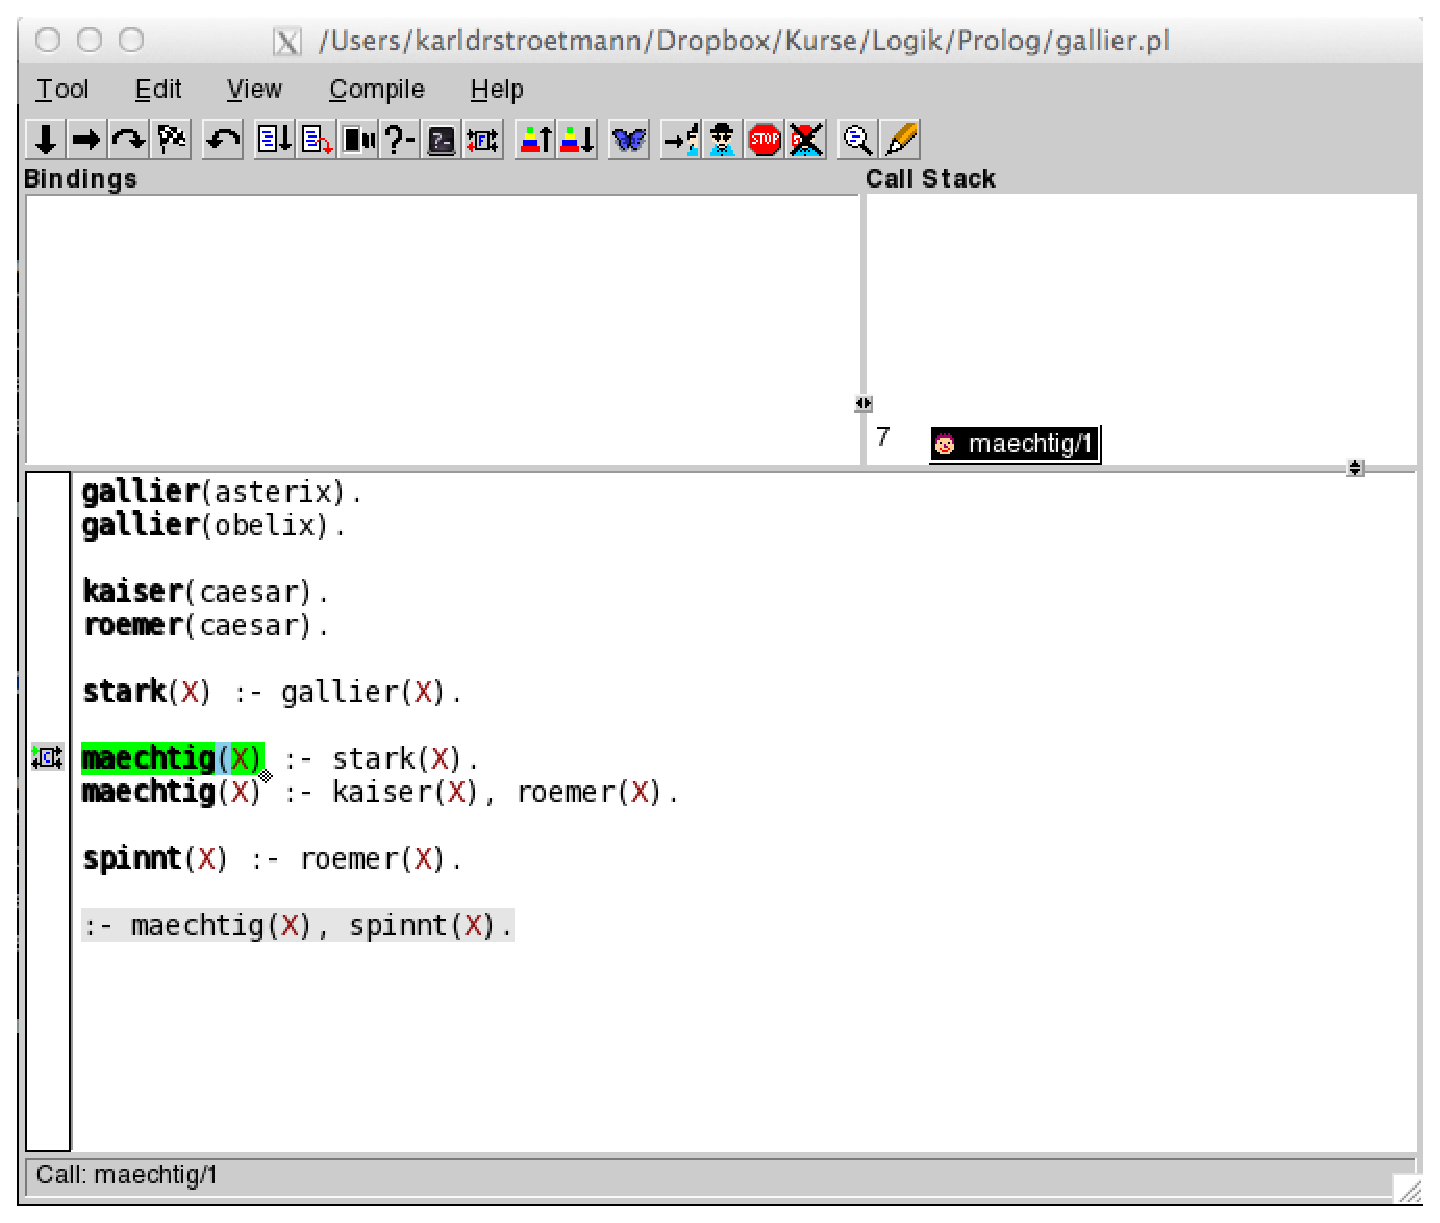
\epsfig{file=Figures/debug.eps,scale=0.7}} 
  \caption{Der Debugger des \textsl{SWI-Prolog}-Systems.}
  \label{fig:debugger}
\end{figure}

Wir zeigen, wie das Ziel \texttt{maechtig(X), spinnt(X)} 
vom \textsl{Prolog}-System beantwortet wird.  
\begin{enumerate}
\item Zun\"{a}chst wird versucht, die Anfrage ``\texttt{maechtig(X)}'' zu l\"{o}sen.
      Die erste Regel, die das Pr\"{a}dikat \texttt{maechtig/1} definiert,
      ist \\[0.2cm]
      \hspace*{1.3cm} \texttt{maechtig(X) :- stark(X).}\\[0.2cm]
      Daher wird die Anfrage ``\texttt{maechtig(X)}'' reduziert zu der Anfrage 
      ``\texttt{stark(X)}''.  Die aktuelle vollst\"{a}ndige Anfrage lautet nun \\[0.2cm]
      \hspace*{1.3cm} \texttt{stark(X), spinnt(X)}. \\[0.2cm]
      Da es noch eine zweite Regel gibt, die das Pr\"{a}dikat \texttt{maechtig/1} definiert,
      setzen wir an dieser Stelle einen Auswahl-Punkt (\emph{Choice-Point}).  Falls also die 
      Beantwortung der Anfrage ``\texttt{stark(X), spinnt(X)}'' sp\"{a}ter scheitert,
      k\"{o}nnen wir es mit der zweiten Regel noch einmal versuchen.
\item Jetzt wird versucht, die Anfrage ``\texttt{stark(X)}'' zu l\"{o}sen.
      Die erste und einzige Regel, die das Pr\"{a}dikat \texttt{stark/1} definiert, ist 
      \\[0.2cm]
      \hspace*{1.3cm} \texttt{stark(X) :- gallier(X).} \\[0.2cm]
      Nach der Unifikation des Kopfes dieser Regel mit der Anfrage ``\texttt{stark(X)}''
      lautet die aktuelle Anfrage \\[0.2cm]
      \hspace*{1.3cm} 
      \texttt{gallier(X), spinnt(X).}
\item Die erste Regel, die das Pr\"{a}dikat \texttt{gallier/1} definiert und deren Kopf
      mit der Anfrage ``\texttt{gallier(X)}'' unifiziert werden kann, ist der Fakt \\[0.2cm]
      \hspace*{1.3cm} \texttt{gallier(asterix).} \\[0.2cm]
      Bei der Unifikation mit diesem Fakt wird die Variable \texttt{X} an die Konstante
      \texttt{asterix} gebunden.  Damit lautet jetzt die aktuelle Anfrage \\[0.2cm]
      \hspace*{1.3cm} 
      \texttt{spinnt(asterix).} \\[0.2cm]
      Da es noch eine zweite Regel gibt, die das Pr\"{a}dikat \texttt{gallier/1} definiert,
      setzen wir an dieser Stelle einen Auswahl-Punkt.   
\item Die erste und einzige Regel, die das Pr\"{a}dikat \texttt{spinnt/1} definiert,
      lautet \\[0.2cm]
      \hspace*{1.3cm} 
      \texttt{spinnt(X) :- roemer(X).} \\[0.2cm]
      Also wird nun die Variable \texttt{X} in dieser Regel mit \texttt{asterix} 
      unifiziert und wir erhalten die Anfrage \\[0.2cm]
      \hspace*{1.3cm} 
      \texttt{roemer(asterix).}
\item Die einzige Regel, die das Pr\"{a}dikat \texttt{roemer/1} definiert, ist \\[0.2cm]
      \hspace*{1.3cm} 
      \texttt{roemer(caesar).} \\[0.2cm]
      Diese Regel l\"{a}sst sich nicht mit der Anfrage ``\texttt{roemer(asterix)}'' unifizieren.
      Also scheitert diese Anfrage.
\item Wir schauen nun, wann wir das letzte mal einen Auswahl-Punkt gesetzt haben.
      Wir stellen fest, dass wir unter Punkt 3 bei der Beantwortung der Anfrage
      \texttt{gallier(X)} das letzte Mal einen Auswahl-Punkt gesetzt haben.
      Also gehen wir nun zu Punkt 3 zur\"{u}ck und versuchen wieder, die Anfrage
      \\[0.2cm]
      \hspace*{1.3cm} 
      \texttt{gallier(X), spinnt(X)} \\[0.2cm]
      zu l\"{o}sen.  Diesmal w\"{a}hlen wir jedoch den Fakt \\[0.2cm]
      \hspace*{1.3cm} \texttt{gallier(obelix).}  \\[0.2cm]
      Wir erhalten dann die neue Anfrage \\[0.2cm]
      \hspace*{1.3cm} \texttt{spinnt(obelix).}
\item Die erste und einzige Regel, die das Pr\"{a}dikat \texttt{spinnt/1} definiert,
      lautet \\[0.2cm]
      \hspace*{1.3cm} 
      \texttt{spinnt(X) :- roemer(X).} \\[0.2cm]
      Also wird die Variable \texttt{X} in dieser Regel mit \texttt{obelix} 
      unifiziert und wir erhalten die Anfrage \\[0.2cm]
      \hspace*{1.3cm} 
      \texttt{roemer(obelix).}
\item Die einzige Regel, die das Pr\"{a}dikat \texttt{roemer/1} definiert, ist \\[0.2cm]
      \hspace*{1.3cm} 
      \texttt{roemer(caesar).} \\[0.2cm]
      Diese Regel l\"{a}sst sich nicht mit der Anfrage ``\texttt{roemer(asterix)}'' unifizieren.
      Also scheitert diese Anfrage.
\item Wir schauen wieder, wann das letzte Mal ein Auswahl-Punkt gesetzt wurde.
      Der unter Punkt 3~gesetzte Auswahl-Punkt wurde vollst\"{a}ndig abgearbeitet, dieser
      Auswahl-Punkt kann uns also nicht mehr helfen.
      Aber unter Punkt 1 wurde ebenfalls ein Auswahl-Punkt gesetzt, denn f\"{u}r das Pr\"{a}dikat
      \texttt{maechtig/1} gibt es die weitere Regel \\[0.2cm]
      \hspace*{1.3cm} \texttt{maechtig(X) :- kaiser(X), roemer(X)}. \\[0.2cm]
      Wenden wir diese Regel an, so erhalten wir die Anfrage \\[0.2cm]
      \hspace*{1.3cm} 
      \texttt{kaiser(X), roemer(X), spinnt(X).}
\item F\"{u}r das Pr\"{a}dikat \texttt{kaiser/1} enth\"{a}lt unsere Datenbank genau einen Fakt:\\[0.2cm]
      \hspace*{1.3cm} \texttt{kaiser(caesar).}  \\[0.2cm]
      Benutzen wir diesen Fakt zur Reduktion unserer Anfrage, so  lautet die neue Anfrage \\[0.2cm]
      \hspace*{1.3cm} 
      \texttt{roemer(caesar), spinnt(caesar).}
\item F\"{u}r das Pr\"{a}dikat \texttt{roemer/1} enth\"{a}lt unsere Datenbank genau einen Fakt:\\[0.2cm]
      \hspace*{1.3cm} \texttt{roemer(caesar).}  \\[0.2cm]
      Benutzen wir diesen Fakt zur Reduktion unserer Anfrage, so  lautet die neue Anfrage \\[0.2cm]
      \hspace*{1.3cm} 
      \texttt{spinnt(caesar).}
\item Die erste und einzige Regel, die das Pr\"{a}dikat \texttt{spinnt/1} definiert,
      lautet \\[0.2cm]
      \hspace*{1.3cm} 
      \texttt{spinnt(X) :- roemer(X).} \\[0.2cm]
      Also wird die Variable \texttt{X} in dieser Regel mit \texttt{caesar} 
      unifiziert und wir erhalten die Anfrage \\[0.2cm]
      \hspace*{1.3cm} 
      \texttt{roemer(caesar).}
\item F\"{u}r das Pr\"{a}dikat \texttt{roemer/1} enth\"{a}lt unsere Datenbank genau einen Fakt:\\[0.2cm]
      \hspace*{1.3cm} \texttt{roemer(caesar).}  \\[0.2cm]
      Benutzen wir diesen Fakt zur Reduktion unserer Anfrage, so ist die verbleibende
      Anfrage leer.  Damit ist die urspr\"{u}ngliche Anfrage gel\"{o}st.  Die dabei berechnete
      Antwort erhalten wir, wenn wir untersuchen, wie die Variable \texttt{X} unifiziert
      worden ist.  Die Variable \texttt{X} war unter Punkt 10 mit der Konstanten
      \texttt{caesar} unifiziert worden.  Also ist \\[0.2cm]
      \hspace*{1.3cm} \texttt{X = caesar}
      \\[0.2cm]
      die Antwort, die von dem System berechnet wird.
\end{enumerate}
Bei der Beantwortung der Anfrage ``\texttt{maechtig(X), spinnt(X)}'' sind wir einige Male
in Sackgassen hineingelaufen und mussten Instantiierungen der Variable \texttt{X} wieder
zur\"{u}ck nehmen.  Dieser Vorgang wird in der Literatur als \emph{backtracking} bezeichnet.
Er kann mit Hilfe des Debuggers am Bildschirm verfolgt werden.

\subsection{Die Tiefensuche}
Der von Prolog verwendete Such-Algorithmus wird auch als \emph{Tiefensuche} (angels\"{a}chsisch:
\emph{depth first search}) bezeichnet.  Um diesen Ausdruck erl\"{a}utern zu k\"{o}nnen, definieren wir
zun\"{a}chst den Begriff des \emph{Suchbaums}.  Die Knoten eines Suchbaums sind mit Anfrage beschriftet.
Ist der Knoten $u$ des Suchbaums mit der Anfrage
\[ Q_1, \cdots, Q_m \]
beschriftet und gibt es f\"{u}r $i = 1,\cdots,k$ Regeln der Form
\[ A^{(i)} \texttt{:-} B_1^{(i)}, \cdots, B_{n(i)}^{(i)} \]
die auf die Anfrage passen, f\"{u}r die also $\mu_i = \textsl{mgu}(Q_1, A^{(i)})$ existiert, so hat der
Knoten $u$ insgesamt $k$ verschiedene Kinder.  Dabei ist das $i$-te Kind mit der Anfrage
\[  B_1^{(i)}\mu_i, \cdots, B_{n(i)}^{(i)}\mu_i, Q_2\mu_i, \cdots, Q_m\mu_i \]
beschriftet.  Als einfaches Beispiel betrachten wir das in Abbildung \ref{fig:depth.pl} gezeigte
Programm.  Der Suchbaum f\"{u}r die Anfrage
\[ p(X) \]
ist in Abbildung \ref{fig:depth-first.eps} gezeigt.  Den Knoten, der mit der urspr\"{u}nglichen Anfrage
beschriftet ist, bezeichnen wir als die \emph{Wurzel} des Suchbaums.  Die \emph{L\"{o}sungen} zu der
urspr\"{u}nglichen Anfrage finden wir an den \emph{Bl\"{a}ttern} des Baumes: Wir bezeichnen hier die Knoten
als Bl\"{a}tter, die am weitesten unten stehen.  Suchb\"{a}ume stehen also gewisserma�en auf dem Kopf: Die
Bl\"{a}tter sind unten und die Wurzeln sind oben\footnote{
Daher werden diese Suchb\"{a}ume auch als australische B\"{a}ume bezeichnet.}.

\begin{figure}[!ht]
\centering
\begin{Verbatim}[ frame         = lines, 
                  framesep      = 0.3cm, 
                  labelposition = bottomline,
                  numbers       = left,
                  numbersep     = -0.2cm,
                  xleftmargin   = 0.8cm,
                  xrightmargin  = 0.8cm,
                ]
    p(X) :- q1(X).
    p(X) :- q2(X).
    
    q1(X) :- r1(X). 
    q1(X) :- r2(X). 
    
    q2(X) :- r3(X). 
    q2(X) :- r4(X). 
    
    r1(a).
    r2(b).
    r3(c).
    r4(d).
\end{Verbatim}
\vspace*{-0.3cm}
\caption{Die Tiefensuche in Prolog}
\label{fig:depth.pl}
\end{figure}

\begin{figure}[!ht]
\centering
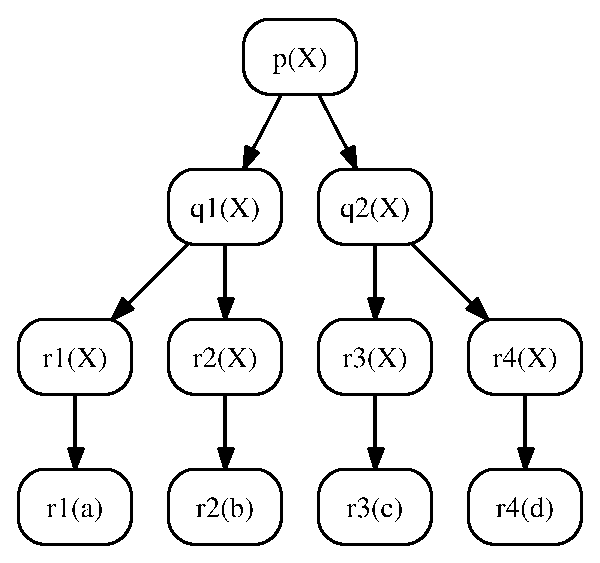
\epsfig{file=depth-first.eps,scale=0.6}

\vspace*{-0.3cm}
\caption{Der Suchbaum f\"{u}r das in Abbildung \ref{fig:depth.pl} gezeigte Programm.}
\label{fig:depth-first.eps}
\end{figure}

Anhand des in Abbildung \ref{fig:depth-first.eps} gezeigten Suchbaums l\"{a}sst sich nun die Tiefensuche
erkl\"{a}ren:  Wenn der Prolog-Interpreter nach einer L\"{o}sung sucht, so w\"{a}hlt er immer den linkesten Ast
und steigt dort so tief wie m\"{o}glich ab.  Dadurch werden die L\"{o}sungen in dem Beispiel in der
Reihenfolge
\[ X = a,\; X = b,\; X = c,\; X = d,\; \]
gefunden.  Die Tiefensuche ist dann problematisch, wenn der linkeste Ast des Suchbaums unendlich
tief ist.  Als Beispiel betrachten wir das  in Abbildung \ref{fig:infinite.pl} gezeigte Prolog-Programm.
Zeichnen wir hier den Suchbaum f\"{u}r die Anfrage
\[ p(X) \]
 so finden wir einen unendlichen Ast, in den der Prolog-Interpreter
absteigt und aus dem er dann mit einem Stack-Overflow wieder zur\"{u}ck kommt.  Vertauschen wir hingegen
die Reihenfolge der Klauseln, so kann das Programm die obige Anfrage beantworten.

\begin{figure}[!ht]
\centering
\begin{Verbatim}[ frame         = lines, 
                  framesep      = 0.3cm, 
                  labelposition = bottomline,
                  numbers       = left,
                  numbersep     = -0.2cm,
                  xleftmargin   = 0.8cm,
                  xrightmargin  = 0.8cm,
                ]
    p(s(X)) :- p(X).
    p(c).
\end{Verbatim}
\vspace*{-0.3cm}
\caption{Eine Endlos-Schleife in \textsl{Prolog}.}
\label{fig:infinite.pl}
\end{figure}

\section{Ein komplexeres Beispiel}
Das obige Beispiel war bewusst einfach gehalten um die Sprache \textsl{Prolog} einzuf\"{u}hren.
Um die M\"{a}chtigkeit des Backtrackings zu demonstrieren, pr\"{a}sentieren wir jetzt ein
komplexeres Beispiel.  Es handelt sich um das folgende R\"{a}tsel:
\begin{enumerate}
\item Drei Freunde belegen den ersten, zweiten und dritten Platz bei einem
      Programmier-Wettbewerb.
\item Jeder der drei hat genau einen Vornamen, genau ein Auto und hat sein Programm
      in genau einer Programmier-Sprache geschrieben.
\item Michael programmiert in \textsc{SetlX} und war besser als der Audi-Fahrer.
\item Julia, die einen Ford Mustang f\"{a}hrt, war besser als der Java-Programmierer.
\item Das Prolog-Programm war am besten.
\item Wer f\"{a}hrt Toyota?
\item In welcher Sprache programmiert Thomas?
\end{enumerate}
Um dieses R\"{a}tsel zu l\"{o}sen, \"{u}berlegen wir uns zun\"{a}chst, wie wir die einzelnen Daten
repr\"{a}sentieren k\"{o}nnen, die in dem R\"{a}tsel eine Rolle spielen.  Zun\"{a}chst ist dort von
Personen die Rede. Jede dieser Personen hat genau einen Vornamen, ein Auto und eine
Programmier-Sprache.   Wir repr\"{a}sentieren Personen daher durch Terme der Form \\[0.2cm]
\hspace*{1.3cm} \texttt{person}(\textsl{Name}, \textsl{Car}, \textsl{Language}). \\[0.2cm]
Dabei bezeichnen \textsl{Name}, \textsl{Car} und \textsl{Language} Konstanten, die aus den
entsprechenden Mengen gew\"{a}hlt werden:
\\[0.2cm]
\hspace*{1.3cm} 
$\textsl{Name} \in \{ \texttt{julia}, \texttt{thomas}, \texttt{michael} \}$, \quad
$\textsl{Car} \in \{ \texttt{ford}, \texttt{toyota}, \texttt{audi} \}$, \\[0.2cm]
\hspace*{1.3cm} 
$\textsl{Language} \in \{ \texttt{java}, \texttt{prolog}, \texttt{setlX} \}$. \\[0.2cm]
Wenn wir Personen durch ein dreistelliges Funktions-Zeichen wie oben gezeigt repr\"{a}sentieren, k\"{o}nnen
wir sofort Pr\"{a}dikate angeben, 
die den Vornamen, die Auto-Marke und die Programmier-Sprache aus einem solchen Term
extrahieren.
\begin{enumerate}
\item Das Pr\"{a}dikat \texttt{first\_name/2} extrahiert den Vornamen: \\[0.2cm]
      \hspace*{1.3cm} \texttt{first\_name(person(Name, Car, Language), Name).}
\item Das Pr\"{a}dikat \texttt{car/2} extrahiert die Auto-Marke: \\[0.2cm]
      \hspace*{1.3cm} \texttt{car(person(Name, Car, Language), Car).}
\item Das Pr\"{a}dikat \texttt{language/2} extrahiert die Programmier-Sprache: \\[0.2cm]
      \hspace*{1.3cm} \texttt{language(person(Name, Car, Language), Language).}
\end{enumerate}
Um zu verstehen wie diese Pr\"{a}dikate arbeiten, zeigen wir, wie die Anfrage \\[0.2cm]
\hspace*{1.3cm} \texttt{car( person(hans, seat, setlX), X ).}\\[0.2cm]
von dem \textsl{Prolog}-System beantwortet wird.  Die einzige Regel, die zur Beantwortung
dieser Anfrage herangezogen werden kann, ist die Regel \\[0.2cm]
\hspace*{1.3cm} \texttt{car(person(Name, Car, Language), Car) :- true.} \\[0.2cm]
Um diese Regel anwenden zu k\"{o}nnen, ist die syntaktische Gleichung \\[0.2cm]
\hspace*{1.3cm} 
$\texttt{car( person(hans, seat, setlX), X )} \doteq \texttt{car( person(Name, Car, Language), Car )}$
\\[0.2cm]
zu l\"{o}sen.  Bei der Unifikation findet sich die L\"{o}sung \\[0.2cm]
\hspace*{1.3cm} 
$\mu = [ \texttt{Name} \mapsto \texttt{hans},\; \texttt{Car} \mapsto \texttt{seat},\;\texttt{Language} \mapsto \texttt{setlX},\; \texttt{X} \mapsto \texttt{seat}]$.
\\[0.2cm]
Insbesondere wird also die Variable \texttt{X} bei dieser Anfrage an die Konstante
\texttt{seat} gebunden.

Wie k\"{o}nnen wir nun die Reihenfolge repr\"{a}sentieren, in der die drei Personen bei dem 
Wettbewerb abgeschnitten haben?  Wir w\"{a}hlen ein dreistelliges Funktions-Zeichen
\texttt{sequence} und repr\"{a}sentieren die Reihenfolge durch den Term
\\[0.2cm]
\hspace*{1.3cm} \texttt{sequence}(\textsl{First}, \textsl{Second}, \textsl{Third}).\\[0.2cm]
Dabei stehen \textsl{First}, \textsl{Second} und \textsl{Third} f\"{u}r Terme, die von dem
Funktions-Zeichen \texttt{person/3} erzeugt worden sind und die Personen bezeichnen.
Die Reihenfolge kann dann durch das Pr\"{a}dikat \\[0.2cm]
\hspace*{1.3cm} \texttt{did\_better}(\textsl{Better}, \textsl{Worse}, \textsl{Sequence})
\\[0.2cm]
berechnet werden, dessen Implementierung in den Zeilen 38 -- 40 der Abbildung
\ref{fig:toyota} auf Seite \pageref{fig:toyota} gezeigt ist.
Wir k\"{o}nnen nun daran gehen, das R\"{a}tsel zu l\"{o}sen.  Abbildung
\ref{fig:toyota} zeigt die Implementierung.
Zeile 1 -- 30 enth\"{a}lt die Implementierung einer Regel f\"{u}r das
Pr\"{a}dikat \texttt{answer/2}, dass die L\"{o}sung des R\"{a}tsel berechnet.  
In dieser Regel haben wir das R\"{a}tsel als pr\"{a}dikatenlogische Formel
codiert.  Wir \"{u}bersetzen diese  Regel jetzt zur\"{u}ck in die Umgangssprache
und zeigen dadurch,  dass das Pr\"{a}dikat \texttt{answer/2} das R\"{a}tsel
korrekt beschreibt.  Die Nummerierung in der folgenden Aufz\"{a}hlung
stimmt jeweils mit der entsprechenden Zeilen-Nummer im Programm \"{u}berein:
\begin{enumerate}
\item[2.] Falls \texttt{Sequence} eine Reihenfolge von drei Personen beschreibt  und
\item[4.] \texttt{Michael} eine Person aus dieser Reihenfolge ist und
\item[5.] der Name der durch \texttt{Michael} bezeichneten Person den Wert \texttt{michael}
         hat und
\item[6.] \texttt{Michael} in \textsc{SetlX} programmiert und
\item[8.] \texttt{Audi} eine Person aus der Reihenfolge \texttt{Sequence} ist und
\item[9.] \texttt{Michael} beim Wettbewerb besser abgeschnitten hat als die durch \texttt{Audi} bezeichnete Person
\item[10.] die durch \texttt{Audi} bezeichnete Person einen Audi f\"{a}hrt und 

           $\vdots$

\item[24.] \texttt{Toyota} eine Person aus der Reihenfolge \texttt{Sequence} ist und
\item[25.] die durch \texttt{Toyota} bezeichnete Person einen Toyota f\"{a}hrt und
\item[26.] \texttt{NameToyota} den Vornamen der durch \texttt{Toyota} bezeichneten Person angibt und
\item[28.] \texttt{Thomas} eine Person aus der Reihenfolge \texttt{Sequence} ist und
\item[25.] die durch \texttt{Thomas} bezeichnete Person den Vornamen Thomas hat und
\item[26.] \texttt{LanguageThomas} die Sprache ist, in der die durch \texttt{Thomas}
          bezeichnete Person programmiert,

          dann gilt:

\item[1.] \texttt{NameToyota} ist der Namen des Toyota-Fahrers und
         \texttt{LanguageThomas} ist die Sprache, in der Thomas programmiert.
\end{enumerate}


\begin{figure}[!h]
  \centering
\begin{Verbatim}[ frame         = lines, 
                  framesep      = 0.3cm, 
                  labelposition = bottomline,
                  numbers       = left,
                  numbersep     = -0.2cm,
                  xleftmargin   = 0.8cm,
                  xrightmargin  = 0.8cm
                ]
    answer(NameToyota, LanguageThomas) :-
        is_sequence( Sequence ),
        % Michael programmiert in SetlX.
        one_of_them(Michael, Sequence),
        first_name(Michael, michael),  
        language(Michael, setlX),
        % Michael war besser als der Audi-Fahrer                     
        one_of_them(Audi, Sequence),
        did_better(Michael, Audi, Sequence),         
        car(Audi, audi),
        % Julia f\"{a}hrt einen Ford Mustang.
        one_of_them(Julia, Sequence),
        first_name(Julia, julia),
        car(Julia, ford), 
        % Julia war besser als der Java-Programmierer.
        one_of_them(JavaProgrammer, Sequence),
        language(JavaProgrammer, java),
        did_better(Julia, JavaProgrammer, Sequence), 
        % Das Prolog-Programm war am besten.
        one_of_them(PrologProgrammer, Sequence),
        first(PrologProgrammer, Sequence),           
        language(PrologProgrammer, prolog),
        % Wer f\"{a}hrt Toyota?
        one_of_them(Toyota, Sequence),
        car(Toyota, toyota),
        first_name(Toyota, NameToyota),              
        % In welcher Sprache programmiert Thomas?
        one_of_them(Thomas, Sequence),
        first_name(Thomas, thomas),
        language(Thomas, LanguageThomas).            
        
    is_sequence( sequence(_First, _Second, _Third) ).
    
    one_of_them(A, sequence(A, _, _)).
    one_of_them(B, sequence(_, B, _)).
    one_of_them(C, sequence(_, _, C)).
    
    did_better(A, B, sequence(A, B, _)).
    did_better(A, C, sequence(A, _, C)).
    did_better(B, C, sequence(_, B, C)).
    
    first(A, sequence(A, _, _)).
    
    first_name(person(Name, _Car, _Language), Name).
    
    car(person(_Name, Car, _Language), Car).
    
    language(person(_Name, _Car, Language), Language).
\end{Verbatim}
\vspace*{-0.3cm}
  \caption{Wer f\"{a}hrt Toyota?}
  \label{fig:toyota}
\end{figure}

Wenn wir die urspr\"{u}ngliche Aufgabe mit der Implementierung in \textsl{Prolog} vergleichen,
dann stellen wir fest, dass die in dem R\"{a}tsel gemachten Angaben eins-zu-eins in
\textsl{Prolog} \"{u}bersetzt werden konnten.  Diese \"{u}bersetzung beschreibt nur das R\"{a}tsel und
gibt keinen Hinweis, wie dieses R\"{a}tsel zu l\"{o}sen ist.  F\"{u}r die L\"{o}sung ist dann die dem
\textsl{Prolog}-System zu Grunde liegende \textsl{Inferenz-Maschine} zust\"{a}ndig.

\section{Listen}
In Prolog wird viel mit Listen gearbeitet.  Listen werden in Prolog mit dem
2-stelligen Funktions-Zeichen ``\texttt{.}'' konstruiert.  Ein Term der Form \\[0.2cm]
\hspace*{1.3cm} \texttt{.($s$,$t$)} \\[0.2cm]
steht also f\"{u}r eine Liste, die als erstes Element ``$s$'' enth\"{a}lt. ``$t$'' bezeichnet den
Rest der Liste.
Das Funktions-Zeichen ``\texttt{[]}'' steht
f\"{u}r die leere Liste. Eine Liste, die aus  den drei Elementen 
``\texttt{a}'', ``\texttt{b}'' und ``\texttt{c}'' besteht, kann also wie folgt dargestellt
werden: \\[0.2cm]
\hspace*{1.3cm} \texttt{.(a, .(b, .(c, [])))} \\[0.2cm]
Da dies relativ schwer zu lesen ist, darf diese Liste auch als \\[0.2cm]
\hspace*{1.3cm} \texttt{[a,b,c]} \\[0.2cm]
geschrieben werden.  Zus\"{a}tzlich kann der Term ``\texttt{.($s$,$t$)}'' in der Form \\[0.2cm]
\hspace*{1.3cm} \texttt{[ $s$ | $t$ ]} \\[0.2cm]
geschrieben werden.  Um diese Kurzschreibweise zu erl\"{a}utern, geben wir ein kurzes
Prolog-Programm an, das zwei Listen aneinander h\"{a}ngen kann.  
Das Programm implementiert das dreistellige Pr\"{a}dikat \texttt{myAppend}\footnote{In dem
  \textsl{SWI-Prolog}-System gibt es das vordefinierte Pr\"{a}dikat \texttt{append/3},
  das genau dasselbe leistet wie unsere Implementierung von \texttt{myAppend/3}.}.  
Die Intention ist,
dass $\texttt{myAppend}(l_1,l_2,l_3)$ f\"{u}r drei Listen $l_1$, $l_2$ und $l_3$ genau dann
wahr sein soll,
wenn die Liste $l_3$ dadurch entsteht, dass die Liste $l_2$ hinten an die Liste $l_1$
angeh\"{a}ngt wird.  Das Programm besteht aus den folgenden beiden Klauseln:
\begin{verbatim}
  myAppend( [], L, L ).
  myAppend( [ X | L1 ], L2, [ X | L3 ] ) :- myAppend( L1, L2, L3 ).
\end{verbatim}
Wir k\"{o}nnen diese beiden Klauseln folgenderma�en in die Umgangssprache \"{u}bersetzen:
\begin{enumerate}
\item H\"{a}ngen wir eine Liste \texttt{L} an die leere Liste an, so ist das Ergebnis die
      Liste \texttt{L}.
\item Um an eine Liste \texttt{[ X | L1 ]}, die aus dem Element \texttt{X} und dem Rest \texttt{L1} besteht,
      eine Liste \texttt{L2} anzuh\"{a}ngen, h\"{a}ngen wir zun\"{a}chst an die Liste \texttt{L1} die 
      Liste \texttt{L2} an und nennen das Ergebnis \texttt{L3}.  
      Das Endergebnis erhalten wir, wenn wir vor die Liste \texttt{L3} noch das Element \texttt{X}
      setzen.  Wir erhalten dann die Liste \texttt{[ X | L3 ]}.
\end{enumerate}
Wir testen unser Programm und nehmen dazu an, dass die beiden Programm-Klauseln in der Datei
``\texttt{myAppend.pl}'' abgespeichert sind und dass wir diese Datei mit dem Befehl ``\texttt{consult(myAppend).}'' geladen haben.
Dann stellen wir die Anfrage \\[0.2cm]
\hspace*{1.3cm} \texttt{?- myAppend( [ 1, 2, 3 ], [ a, b, c ], L ).} \\[0.2cm]
Wir erhalten die Antwort:
\begin{verbatim}
    L = [1, 2, 3, a, b, c] 
\end{verbatim}
Die obige Interpretation des gegebenen Prolog-Programms ist \emph{funktional}, dass hei�t 
wir fassen die ersten beiden Argumente des Pr\"{a}dikats \texttt{myAppend} als \emph{Eingaben} auf und 
interpretieren das letzte Argument als \emph{Ausgabe}.  Diese Interpretation ist aber keineswegs die 
einzig m\"{o}gliche Interpretation.  Um das zu sehen, geben wir als Ziel \\[0.2cm]
\hspace*{1.3cm} \texttt{myAppend(L1, L2, [1,2,3]).} \\[0.2cm]
ein und dr\"{u}cken, nachdem das System uns die erste Antwort gegeben hat, nicht die Taste 
\textsl{Return} sondern die Taste ``\texttt{;}''.  Wir erhalten:
\begin{verbatim}
    ?- myAppend(L1, L2, [1, 2, 3]).

    L1 = []
    L2 = [1, 2, 3] ;

    L1 = [1]
    L2 = [2, 3] ;

    L1 = [1, 2]
    L2 = [3] ;

    L1 = [1, 2, 3]
    L2 = [] ;

    No
\end{verbatim}
In diesem Fall hat das Prolog-System durch Backtracking  alle M\"{o}glichkeiten bestimmt, die
es gibt, um die Liste ``\texttt{[1, 2, 3]}'' in zwei Teillisten zu zerlegen.

\subsection{Sortieren durch Einf\"{u}gen}
Wir entwickeln nun einen einfachen Algorithmus zum Sortieren von Listen von Zahlen.
Die Idee ist Folgende:  Um eine Liste aus $n$ Zahlen zu sortieren, sortieren wir zun\"{a}chst
die letzten $n-1$ Zahlen und f\"{u}gen dann das erste Element an der richtigen Stelle in die sortierte
Liste ein.  Mit dieser Idee besteht das Programm aus zwei Pr\"{a}dikaten:
\begin{enumerate}
\item Das Pr\"{a}dikat \texttt{insert/3} erwartet
      als erstes Argument eine Zahl $x$ und als zweites Argument eine Liste von Zahlen $l$,
      die bereits in aufsteigender Reihenfolge sortiert ist.  
      Das Pr\"{a}dikat f\"{u}gt die Zahl $x$ so in die Liste $l$ ein, dass die resultierende Liste
      ebenfalls in aufsteigender Reihenfolge sortiert ist. Das so berechnete Ergebnis
      wird als letztes Argument des Pr\"{a}dikats \texttt{insert/3} zur\"{u}ck gegeben.  

      Um die obigen Ausf\"{u}hrungen
      \"{u}ber die verwendeten Typen und die Bestimmung von Ein- und Ausgabe pr\"{a}gnanter
      formulieren zu k\"{o}nnen, f\"{u}hren wir den Begriff einer \emph{Typ-Spezifikation} ein.
      F\"{u}r das Pr\"{a}dikat \texttt{insert/3} hat diese Typ-Spezifikation die Form \\[0.2cm]
      \hspace*{1.3cm} 
      \texttt{insert(+\textsl{Number}, +\textsl{List}(\textsl{Number}), -\textsl{List}(\textsl{Number}))}.
      \\[0.2cm]
      Das Zeichen ``\texttt{+}'' legt dabei fest, dass das entsprechende
      Argument eine Eingabe ist, w\"{a}hrend ``\texttt{-}'' verwendet wird um ein
      Ausgabe-Argument zu spezifizieren.
\item Das Pr\"{a}dikat \texttt{insertion\_sort/2} hat die Typ-Spezifikation \\[0.2cm]
      \hspace*{1.3cm} \texttt{insertion\_sort(+\textsl{List}(\textsl{Number}), -\textsl{List}(\textsl{Number}))}.
      \\[0.2cm]
      Der Aufruf \texttt{insertion\_sort}(\textsl{List}, \textsl{Sorted}) sortiert die als Eingabe
      gegebene Liste \textsl{List} in aufsteigender Reihenfolge.
\end{enumerate}


\begin{figure}[!h]
  \centering
\begin{Verbatim}[ frame         = lines, 
                  framesep      = 0.3cm, 
                  labelposition = bottomline,
                  numbers       = left,
                  numbersep     = -0.2cm,
                  xleftmargin   = 0.8cm,
                  xrightmargin  = 0.8cm
                ]
    % insert( +Number, +List(Number), -List(Number) ).

    insert( X, [], [ X ] ). 

    insert( X, [ Head | Tail ], [ X, Head | Tail ] ) :-
        X =< Head.

    insert( X, [ Head | Tail ], [ Head | New_Tail ] ) :-
        X > Head,
        insert( X, Tail, New_Tail ).

    % insertion_sort( +List(Number), -List(Number) ).

    insertion_sort( [], [] ).

    insertion_sort( [ Head | Tail ], Sorted ) :-
        insertion_sort( Tail, Sorted_Tail ),
        insert( Head, Sorted_Tail, Sorted ).
\end{Verbatim}
\vspace*{-0.3cm}
  \caption{Sortieren durch Einf\"{u}gen.}
  \label{fig:insertion-sort}
\end{figure}

Abbildung \ref{fig:insertion-sort} auf Seite \pageref{fig:insertion-sort} zeigt das \textsl{Prolog}-Programm. 
Nachfolgend diskutieren wir die einzelnen Klauseln der Implementierung des Pr\"{a}dikats \texttt{insert}.
\begin{enumerate}
\item Die erste Klausel des Pr\"{a}dikats \texttt{insert} greift, wenn die Liste, in welche die
      Zahl \texttt{X} eingef\"{u}gt werden soll, leer ist.
      In diesem Fall wird als Ergebnis einfach die Liste zur\"{u}ck gegeben, die als einziges Element
      die Zahl \texttt{X} enth\"{a}lt.
\item Die zweite Klausel greift, wenn die Liste, in die die Zahl  \texttt{X} eingef\"{u}gt
      werden soll, nicht leer ist und wenn au�erdem
       \texttt{X} kleiner oder gleich dem ersten Element dieser Liste ist.  In diesem Fall kann \texttt{X} an den Anfang der 
      Liste gestellt werden. Dann erhalten wir die Liste \\[0.2cm]
      \hspace*{1.3cm} \texttt{[ X, Head | Tail ]}. \\[0.2cm]
      Diese Liste ist sortiert, weil einerseits schon die Liste \texttt{[ Head | Tail ]} sortiert ist
      und andererseits \texttt{X} kleiner als \texttt{Head} ist.
\item Die dritte Klausel greift, wenn die Liste, in die die Zahl  \texttt{X} eingef\"{u}gt
      werden soll  nicht leer ist und wenn au�erdem \texttt{X} gr\"{o}�er als das erste
      Element dieser Liste ist.  In diesem Fall muss \texttt{X} rekursiv
      in die Liste \texttt{Tail} eingef\"{u}gt werden.  Dabei bezeichnet \texttt{Tail} den
      Rest der Liste, in die wir \texttt{X} einf\"{u}gen wollen.
      Weiter bezeichnet \texttt{New\_Tail} die Liste, die wir erhalten, wenn wir die Zahl
      \texttt{X} in die Liste \texttt{Tail} einf\"{u}gen.
      An den Anfang der  Liste \texttt{New\_Tail} setzen wir nun noch den Kopf
      \texttt{Head} der als Eingabe gegebenen Liste.
\end{enumerate}
Damit k\"{o}nnen wir nun auch die Wirkungsweise des Pr\"{a}dikats \texttt{insertion\_sort} erkl\"{a}ren.
\begin{enumerate}
\item Ist die zu sortierende Liste leer, so ist das Ergebnis die leere Liste.
\item Ist die zu sortierende Liste nicht leer und hat die Form \texttt{[Head | Tail]}, so sortieren wir zun\"{a}chst die
      Liste \texttt{Tail} und erhalten als Ergebnis die sortierte Liste \texttt{Sorted\_Tail}.  F\"{u}gen wir hier
      noch das Element \texttt{Head} mit Hilfe von \texttt{insert} ein, so erhalten wir als Endergebnis
      die sortierte Liste.
\end{enumerate}
Viele \textsl{Prolog}-Pr\"{a}dikate sind \emph{funktional}.  
Wir nennen ein Pr\"{a}dikat funktional,
wenn die einzelnen Argumente klar in Eingabe- und Ausgabe-Argumente unterschieden werden
k\"{o}nnen und wenn au�erdem zu jeder Eingabe h\"{o}chstens eine Ausgabe berechnet wird.
Zum Beispiel sind die oben angegebenen Pr\"{a}dikate zum Sortieren einer Liste von Zahlen funktional.
Bei einem funktionalen Programm k\"{o}nnen wir die Semantik oft dadurch am besten verstehen,
dass wir das Programm in \emph{bedingte Gleichungen} umformen.  F\"{u}r das oben angegebene
Programm erhalten wir dann die folgenden Gleichungen:
\begin{enumerate}
\item $\texttt{insert}( \textsl{X}, []) = [ \textsl{X} ]$. 
\item $\textsl{X} \leq \texttt{\textsl{Head}} \rightarrow \texttt{insert}(\textsl{X}, [ \textsl{Head} | \textsl{Tail} ]) =  [ \textsl{X}, \textsl{Head} | \textsl{Tail} ]$.
\item $\textsl{X} > \texttt{\textsl{Head}} \rightarrow \texttt{insert}(\textsl{X}, [ \textsl{Head} | \textsl{Tail} ]) =  [ \textsl{Head} | \texttt{insert}(\textsl{X}, \textsl{Tail}) ]$.
\item $\texttt{insertion\_sort}([]) = []$.
\item $\texttt{insertion\_sort}([ \textsl{Head} | \textsl{Tail} ]) = \texttt{insert}(\textsl{Head}, \texttt{insertion\_sort}(\textsl{Tail}))$.
\end{enumerate}
Die Korrespondenz zwischen dem \textsl{Prolog}-Programm und den Gleichungen sollte
augenf\"{a}llig sein.  Au�erdem ist offensichtlich, dass die obigen Gleichungen 
den Sortier-Algorithmus in sehr pr\"{a}gnanter Form wiedergeben.  Wir werden diese Beobachtung
im zweiten Semester benutzen und die meisten dort vorgestellten Algorithmen durch bedingte
Gleichungen spezifizieren. 

\subsection{Sortieren durch Mischen}
Der im letzten Abschnitt vorgestellte Sortier-Algorithmus hat einen Nachteil:  Die Rechenzeit,
die dieser Algorithmus verbraucht, w\"{a}chst im ung\"{u}nstigsten Fall quadratisch mit der L\"{a}nge der zu sortierenden 
Liste.  Den Beweis dieser Behauptung werden wir im n\"{a}chsten Semester liefern.
Wir werden nun einen Algorithmus vorstellen der effizienter ist:  Ist $n$ die L\"{a}nge der
Liste, so w\"{a}chst bei diesem Algorithmus der Verbrauch der 
Rechenzeit nur mit dem Faktor $n \cdot \textsl{log}_2(n)$.  Den Nachweis dieser Behauptung
erbringen wir im zweiten Semester.
Wenn es sich bei der zu sortierenden Liste beispielsweise um ein Telefonbuch mit einer
Millionen Eintr\"{a}gen handelt, dann ist der relative Unterschied zwischen $n^2$ und $n \log_2(n)$ bei
etwa $50\,000$. 

Wir werden den effizienteren Algorithmus zun\"{a}chst durch bedingte Gleichungen beschreiben und
anschlie�end die Umsetzung dieser Gleichungen in \textsl{Prolog} angeben.
Der Algorithmus wird in der Literatur als \emph{Sortieren durch Mischen} bezeichnet
(engl. \emph{merge sort}) und besteht aus drei Phasen:
\begin{enumerate}
\item In der ersten Phase wird die zu sortierende Liste in zwei etwa gleich gro�e
      Teillisten aufgeteilt.
\item In der zweiten Phase werden diese Teillisten rekursiv sortiert.
\item In der dritten Phase werden die sortierten Teillisten so zusammen gef\"{u}gt (gemischt),
      dass die resultierende Liste ebenfalls sortiert ist.
\end{enumerate}

Wir beginnen mit dem Aufteilen einer Liste in zwei Teile.  Bei der Aufteilung orientieren wir
uns an den Indizes der Elemente.  Zur Illustration zun\"{a}chst ein Beispiel: Wir teilen die Liste \\[0.2cm]
\hspace*{1.3cm} 
$[a_1, a_2, a_3, a_4, a_5, a_6, a_7, a_8]$ \quad auf in \quad
$[a_1, a_3, a_5, a_7]$ \quad und \quad $[a_2, a_4, a_6, a_8]$.
\\[0.2cm]
Elemente, deren Index gerade ist, werden in der ersten
Teilliste aufgesammelt und die Elemente mit ungeradem Index sammeln wir in der zweiten
Teilliste.  Als Namen f\"{u}r die  Funktionen, die diese Teillisten berechnen, w\"{a}hlen 
wir \texttt{even} und \texttt{odd}: \\[0.2cm]
\hspace*{1.3cm} 
$\texttt{odd}: \textsl{List}(\textsl{Number}) \rightarrow \textsl{List}(\textsl{Number})$,
\\[0.2cm]
\hspace*{1.3cm} 
$\texttt{even}: \textsl{List}(\textsl{Number}) \rightarrow \textsl{List}(\textsl{Number})$.
\\[0.2cm]
Die Funktion $\texttt{odd}(L)$ berechnet die Liste aller Elemente aus $L$ mit ungeradem Index, 
w\"{a}hrend $\mathtt{even}(L)$ die Liste aller Elemente mit geradem Index berechnet.
Die beiden Funktionen k\"{o}nnen durch die folgenden Gleichungen spezifiziert werden:
\begin{enumerate}
\item $\texttt{odd}([]) = []$.
\item $\texttt{odd}([h|t]) = [h|\texttt{even}(t)]$,

      denn das erste Element einer Liste hat den Index 1, was offenbar ein ungerader Index
      ist und alle Elemente, die in der Liste $t$ einen geraden Index haben, haben in der
      Liste $[h|t]$ einen ungeraden Index.
\item $\texttt{even}([]) = []$.
\item $\texttt{even}([h|t]) = \texttt{odd}(t)$,

      denn alle Elemente, die in der Liste $t$ einen ungeraden Index haben, haben in der Liste
      $[h|t]$ einen geraden Index.
\end{enumerate}
Als n\"{a}chstes entwickeln wir eine Funktion \\[0.2cm]
\hspace*{1.3cm} $\texttt{mix}: \textsl{List}(\textsl{Number}) \times \textsl{List}(\textsl{Number}) \rightarrow \textsl{List}(\textsl{Number})$
\\[0.2cm]
die zwei aufsteigend sortierte Listen so mischt,  dass die resultierende Liste ebenfalls
aufsteigend sortiert ist.  Durch rekursive Gleichungen kann diese Funktion wie folgt
spezifiziert werden: 
\begin{enumerate}
\item $\texttt{mix}([], l) = l$.
\item $\texttt{mix}(l, []) = l$.
\item $x \leq y \rightarrow \texttt{mix}([x|s], [y|t]) = [x|\texttt{mix}(s, [y|t])]$.

      Falls $x \leq y$ ist, so ist $x$ sicher das kleinste Element
      der Liste, die entsteht, wenn wir die bereits sortierten Listen $[x|s]$ und $[y|t]$ mischen.
      Also mischen wir rekursiv die Listen $s$ und $[y|t]$ und setzen $x$ an den Anfang
      dieser Liste.
\item $x  >   y \rightarrow \texttt{mix}([x|s], [y|t]) = [y|\texttt{mix}([x|s], t)]$.
\end{enumerate}
Damit k\"{o}nnen wir jetzt die Funktion\\[0.2cm]
\hspace*{1.3cm}  $\texttt{merge\_sort}: \textsl{List}(\textsl{Number}) \rightarrow \textsl{List}(\textsl{Number})$,
\\[0.2cm]
die eine Liste von Zahlen sortiert, durch bedingte Gleichungen spezifizieren.
\begin{enumerate}
\item $\texttt{merge\_sort}([]) = []$.
\item $\texttt{merge\_sort}([x]) = [x]$.
\item $\mathtt{length}(l) \geq 2 \rightarrow \texttt{merge\_sort}(l) = \texttt{mix}(
  \texttt{merge\_sort}(\texttt{odd}(l)),
  \texttt{merge\_sort}(\texttt{even}(l)))$.

      Falls die Liste $l$ aus 2 oder mehr Elementen besteht, teilen wir diese Liste
      in die beiden Listen $\mathtt{odd}(l)$ und $\mathtt{even}(l)$ auf, sortieren 
      diese Listen und mischen anschlie�end die sortierten Teillisten.
\end{enumerate}
Die oben angegebenen Gleichungen lassen sich nun unmittelbar in ein
\textsl{Prolog}-Programm umsetzen.  Abbildung \ref{fig:merge-sort}
auf Seite \pageref{fig:merge-sort} zeigt das resultierende \textsl{Prolog}-Programm.
Da es in \textsl{SWI-Prolog} bereits vordefinierte Pr\"{a}dikate mit den Namen 
\texttt{merge/3} und \texttt{sort/2} gibt, habe ich statt dessen die Namen
\texttt{mix/2} und \texttt{merge\_sort/3} gew\"{a}hlt.


\begin{figure}[!h]
  \centering
\begin{Verbatim}[ frame         = lines, 
                  framesep      = 0.3cm, 
                  labelposition = bottomline,
                  numbers       = left,
                  numbersep     = -0.2cm,
                  xleftmargin   = 0.8cm,
                  xrightmargin  = 0.8cm
                ]
    % odd( +List(Number), -List(Number) ).
    odd( [], [] ).    
    odd( [ X | Xs ], [ X | L ] ) :-
        even( Xs, L ).
    
    % even( +List(Number), -List(Number) ).
    even( [], [] ).
    even( [ _X | Xs ], L ) :-
        odd( Xs, L ).
    
    % merge( +List(Number), +List(Number), -List(Number) ).
    mix( [], Xs, Xs ).    
    mix( Xs, [], Xs ).
    mix( [ X | Xs ], [ Y | Ys ], [ X | Rest ] ) :-
        X =< Y,
        mix( Xs, [ Y | Ys ], Rest ).    
    mix( [ X | Xs ], [ Y | Ys ], [ Y | Rest ] ) :-
        X > Y,
        mix( [ X | Xs ], Ys, Rest ).
    
    % merge_sort( +List(Number), -List(Number) ).    
    merge_sort( [], [] ).
    merge_sort( [ X ], [ X] ).    
    merge_sort( [ X, Y | Rest ], Sorted ) :-
        odd(  [ X, Y | Rest ], Odd  ),
        even( [ X, Y | Rest ], Even ),
        merge_sort( Odd,  Odd_Sorted  ),
        merge_sort( Even, Even_Sorted ),
        mix( Odd_Sorted, Even_Sorted, Sorted ).
\end{Verbatim}
\vspace*{-0.3cm}
  \caption{Sortieren durch Mischen.}
  \label{fig:merge-sort}
\end{figure}


\subsection{Symbolisches Differenzieren}
Die Sprache \textsl{Prolog} wird gerne f\"{u}r Anwendungen benutzt, bei denen symbolische
Rechnungen eine wesentliche Rolle spielen, denn 
symbolische Rechnungen sind in \textsl{Prolog} dadurch, dass die zu
manipulierenden Objekte in der Regel unmittelbar als Prolog-Terme dargestellt werden
k\"{o}nnen, sehr einfach zu implementieren.  Zur Verdeutlichung zeigen wir ein Programm, mit
dem es m\"{o}glich ist, symbolisch zu differenzieren. 
Im Rahmen einer \"{u}bung haben wir ein \textsc{SetlX}-Programm entwickelt, das arithmetische Ausdr\"{u}cke
symbolisch differenziert.  Damals hatten wir davon profitiert, dass die Sprache \textsc{SetlX} Terme
als Datenstruktur zur Verf\"{u}gung stellt.  Da in der Sprache \textsl{Prolog} Terme ebenfalls fest
eingebaut sind, ist es in
\textsl{Prolog} genauso einfach, symbolisch zu differenzieren.

Die Methodik, mit der wir das \textsl{Prolog}-Programm entwickeln, besteht aus zwei
Schritten:
\begin{enumerate}
\item Als erstes legen wir fest, was genau wir unter einem arithmetischen Ausdruck
      verstehen wollen und wie ein solcher Ausdruck in \textsl{Prolog} repr\"{a}sentiert werden soll.  
      Dazu definieren wir die Menge der \textsl{Prolog}-Terme \textsl{Expr}, 
      die einen arithmetischen Ausdruck darstellen.
\item Dann stellen wir bedingte Gleichungen auf, die eine Funktion
      \[ \texttt{diff}: \textsl{Expr} \times \textsl{Var} \rightarrow \textsl{Expr} \]
      beschreiben.  Diese Gleichungen sind nichts anderes als die mathematischen Regeln,
      die Sie in der Schule f\"{u}r das Differenzieren gelernt haben.
\item Im letzten Schritt implementieren wir diese Gleichungen in Prolog.
\end{enumerate}

\paragraph{Induktive Definition der Menge \textsl{Expr}.}
\begin{enumerate}
\item Variablen sind arithmetische Ausdr\"{u}cke.

      Variablen stellen wir durch nullstellige Funktionszeichen dar.
      Nullstellige Funktionszeichen werden in Prolog auch als \emph{Atome} bezeichnet.
      Damit gilt
      \[ c \in \textsl{Expr} \quad \mbox{f\"{u}r jedes \textsl{Prolog}-Atom $c$}. \]
\item Zahlen sind arithmetische Ausdr\"{u}cke.

      Sowohl die ganzen Zahlen als auch die Flie�komma-Zahlen sind Bestandteil der Sprache
      \textsl{Prolog} und k\"{o}nnen damit durch sich selbst dargestelt werden:
      \[ n \in \textsl{Expr} \quad \mbox{f\"{u}r alle $n \in \mathbb{Z}$}, \]
      \[ r \in \textsl{Expr} \quad \mbox{f\"{u}r alle $r \in \mathbb{R}$}. \]
\item Das Negative eines arithmetischen Ausdrucks ist ein arithmetischer Ausdruck.
      In \textsl{Prolog} kann das Negative durch den un\"{a}ren Operator ``\texttt{-}'' dargestellt
      werden, also haben wir
      \[ \texttt{-}\; t \in \textsl{Expr} \quad \mbox{falls $t \in \textsl{Expr}$}. \]
\item Die Summe, die Differenz, das Produkt, und der Quotient zweier arithmetischen
      Ausdr\"{u}cke ist ein arithmetischer Ausdruck. 
      In \textsl{Prolog} k\"{o}nnen Summe, Differenz, Produkt und Quotient respektive
      durch die bin\"{a}ren Operatoren ``\texttt{+}'', ``\texttt{-}'', ``\texttt{*}'' und ``\texttt{/}'' 
      dargestellt werden, also setzen wir
      \[ s \;\texttt{+}\, t \in \textsl{Expr} \quad \mbox{falls $s,t \in \textsl{Expr}$}. \]
      \[ s \;\texttt{-}\; t \in \textsl{Expr} \quad \mbox{falls $s,t \in \textsl{Expr}$}. \]
      \[ s \;\texttt{*}\; t \in \textsl{Expr} \quad \mbox{falls $s,t \in \textsl{Expr}$}. \]
      \[ s \;\texttt{/}\; t \in \textsl{Expr} \quad \mbox{falls $s,t \in \textsl{Expr}$}. \]
\item Die Potenz zweier arithmetischer Ausdr\"{u}cke ist ein arithmetischer Ausdruck.
      In \textsl{Prolog} kann die Potenz durch den bin\"{a}ren Operator ``\texttt{**}'' dargestellt
      werden, also setzen wir
      \[ s \;\texttt{**}\; t \in \textsl{Expr} \quad \mbox{falls $s,t \in \textsl{Expr}$}. \]
\item Bei der Behandlung spezieller Funktionen beschr\"{a}nken wir uns auf die
      Exponential-Funktion und den nat\"{u}rlichen Logarithmus:
      \[ \texttt{exp}(t) \in \textsl{Expr}  \quad \mbox{falls $t \in \textsl{Expr}$}, \]
      \[ \texttt{ln}(t)  \in \textsl{Expr}  \quad \mbox{falls $t \in \textsl{Expr}$}. \]
\end{enumerate}

\paragraph{Aufstellen der bedingten Gleichungen}
Den Wert von $\texttt{diff}(t,x)$ definieren wir nun durch Induktion nach dem Aufbau des
arithmetischen Ausdrucks $t$.
\begin{enumerate}
\item Bei der Ableitung einer Variablen m\"{u}ssen wir unterscheiden,
      ob wir die Variable nach sich selbst oder nach einer anderen Variablen ableiten.
      \begin{enumerate}
      \item Die Ableitung einer Variablen nach sich selbst gibt den Wert 1:
            \[ y = x \rightarrow \bruch{d\,y}{dx} = 1. \]
            Also haben wir 
            \[ y = x \rightarrow \texttt{diff}(y,x) = 1. \]
      \item Die Ableitung einer Variablen $y$ nach einer anderen Variablen $x$ ergibt den Wert 0:
            \[ y \not= x \rightarrow \bruch{d\,y}{dx} = 0 \]
             Also haben wir 
            \[ y \not= x \rightarrow \texttt{diff}(y,x) = 0. \]
      \end{enumerate}
\item Die Ableitung einer Zahl $n$ ergibt 0: 
      \[ \bruch{d\,n}{dx} = 0.  \]
      Damit haben wir
      \[ \texttt{diff}(n, x) = 0. \]
\item Die Ableitung eines Ausdrucks mit negativen Vorzeichen ist durch 
      \[ \bruch{d}{dx}(-f) = - \bruch{d\,f}{dx} \]
      gegeben.  Die rekursive Gleichung lautet 
      \[ \texttt{diff}(-f,x) = - \texttt{diff}(f,x). \]
\item Die Ableitung einer Summe ergibt sich als Summe der Ableitungen der Summanden: 
      \[ \bruch{d}{dx}(f+g) = \bruch{d\,f}{dx} + \bruch{d\,g}{dx} \]
      Als Gleichung schreibt sich dies 
      \[ \texttt{diff}(f + g, x) = \texttt{diff}(f,x) + \texttt{diff}(g,x). \]
\item Die Ableitung einer Differenz ergibt sich als Differenz der Ableitung der Operanden: 
      \[ \bruch{d}{dx}(f-g) = \bruch{d\,f}{dx} - \bruch{d\,g}{dx} \]
      Als Gleichung schreibt sich dies 
      \[ \texttt{diff}(f - g, x) = \texttt{diff}(f,x) - \texttt{diff}(g,x). \]
\item Die Ableitung eines Produktes wird durch die Produkt-Regel beschrieben: 
      \[ \bruch{d}{dx}(f*g) = \bruch{d\,f}{dx}*g + f*\bruch{d\,g}{dx}. \]
      Dies f\"{u}hrt auf die Gleichung 
      \[ \texttt{diff}(f*g,x) = \texttt{diff}(f,x) * g + f * \texttt{diff}(g,x). \]
\item Die Ableitung eines Quotienten wird durch die Quotienten-Regel beschrieben: 
      \[ \bruch{d}{dx}(f/g) = \bruch{\;\displaystyle \rule[-10pt]{0pt}{12pt}
         \bruch{d\,f}{dx}*g - f*\bruch{d\,g}{dx}\;}{\displaystyle \rule{0pt}{10pt}g*g}. \]
      Dies f\"{u}hrt auf die Gleichung 
      \[ \texttt{diff}(f/g,x) = (\texttt{diff}(f,x) * g - f * \texttt{diff}(g,x)) / (g*g). \]
\item Zur Ableitung eines Ausdrucks der Form $f \,\mathtt{**}\, g$ verwenden wir die folgende Gleichung:
      \\[0.2cm]
      \hspace*{1.3cm}      
      $f \,\mathtt{**}\, g = \texttt{exp}(g*\texttt{ln}(f))$.
      \\[0.2cm]
      Das f\"{u}hrt auf die Gleichung 
      \[ 
         \texttt{diff}(f \;\texttt{**}\; g, x) = 
         \texttt{diff}(\mathtt{exp}(g * \mathtt{ln}(f)), x). 
      \]
\item Bei der Ableitung der Exponential-Funktion ben\"{o}tigen wir die Ketten-Regel:
      \[ \bruch{d}{dx}\textsl{exp}(f) = \bruch{d\,f}{dx}* \textsl{exp}(f). \]
      Das f\"{u}hrt auf die Gleichung 
      \[ \texttt{diff}(\texttt{exp}(f), x) = \texttt{diff}(f,x) * \texttt{exp}(f). \]
\item F\"{u}r die Ableitung des nat\"{u}rlichen Logarithmus finden wir unter Ber\"{u}cksichtigung der Ketten-Regel
      \[ \bruch{d}{dx}\textsl{ln}(f) = \bruch{1}{f}*\bruch{d\,f}{dx}. \]
      Das f\"{u}hrt auf die Gleichung 
      \[ \texttt{diff}(\texttt{exp}(f), x) = \texttt{diff}(f,x)/f. \]
\end{enumerate}

\paragraph{Implementierung in \textsl{Prolog}}
Abbildung \ref{fig:symbolisch-diff} zeigt die Implementierung in \textsl{Prolog}.
An Stelle der zweistelligen Funktion $\textsl{diff}()$ haben wir nun ein dreistelliges Pr\"{a}dikat 
\texttt{diff/3}, dessen letztes Argument das Ergebnis berechnet.
Wir diskutieren die einzelnen Klauseln.
\begin{enumerate}
\item Die beiden Klauseln in den Zeilen 3 -- 9 zeigen, wie eine Variable differenziert werden kann.
      Das Pr\"{a}dikat $\texttt{atom}(X)$ pr\"{u}ft, ob $X$ ein nullstelliges Funktions-Zeichen ist.
      Solche Funktions-Zeichen werden im \textsl{Prolog}-Jargon auch als \emph{Atome} bezeichnet.
      Wir pr\"{u}fen also in Zeile 4 und 8, ob es sich bei dem abzuleitenden Ausdruck um eine Variable
      handelt.  Anschlie�end \"{u}berpr\"{u}fen wir in den Zeilen 5 bzw.~9, ob diese Variable mit der
      Variablen, nach der differenziert werden soll, \"{u}bereinstimmt oder nicht.

      
\item In der Klausel in den Zeilen 11 -- 12 behandeln wir den Fall, dass es sich bei dem zu
      differenzierenden Ausdruck um eine Zahl handelt.  Um dies \"{u}berpr\"{u}fen zu k\"{o}nnen, verwenden wir
      das Pr\"{a}dikat \texttt{number(X)}, das \"{u}berpr\"{u}ft, ob das Argument \texttt{X}  eine Zahl ist.
      
      In dieser Klausel haben wir die Variable, nach der abgeleitet werden soll, mit
      ``\texttt{\_X}'' bezeichnet.  Der Grund ist, dass das \textsl{Prolog}-System f\"{u}r Variablen, 
      die in einer Klausel nur einmal vorkommen, eine Warnung ausgibt.  Diese Warnung kann vermieden
      werden, wenn vorne an den Variablennamen  ein Unterstrichs ``\texttt{\_}'' angef\"{u}gt wird.
\item Am Beispiel der Ableitung des Ausdrucks $-f$ zeigen wir, wie rekursive Gleichungen
      in \textsl{Prolog} umgesetzt werden k\"{o}nnen. Die Gleichung, die in den Zeilen 14 --
      15 umgesetzt wird, lautet
      \[ \texttt{diff}(-f,x) = - \texttt{diff}(f,x). \]
      Um den Ausdruck \texttt{-F} nach $x$ zu differenzieren, m\"{u}ssen wir zun\"{a}chst den
      Ausdruck \texttt{F} nach $x$ ableiten.  Das passiert in 
      Zeile 15 und liefert das Ergebnis \texttt{Fs}.  Das Endergebnis erhalten wir dadurch, dass
      wir vor \texttt{Fs} ein Minuszeichen setzen.
\item Die restlichen Klausel setzen die oben gefundenen bedingten Gleichungen unmittelbar um und
      werden daher hier nicht weiter diskutiert.
\end{enumerate}

\begin{figure}[!h]
  \centering
\begin{Verbatim}[ frame         = lines, 
                  framesep      = 0.3cm, 
                  labelposition = bottomline,
                  numbers       = left,
                  numbersep     = -0.2cm,
                  xleftmargin   = 0.8cm,
                  xrightmargin  = 0.8cm
                ]
    % diff( +Expr, +Atom, -Expr).
    
    diff(F, X, 1) :- 
        atom(F), 
        F == X.
    
    diff(F, X, 0) :- 
        atom(F),
        F \== X.
        
    diff(N, _X, 0) :-
        number(N).
    
    diff(-F, X, -Fs) :-
        diff(F, X, Fs).
    
    diff(F + G, X, Fs + Gs) :-
        diff(F, X, Fs),
        diff(G, X, Gs).
    
    diff(F - G, X, Fs - Gs) :-
        diff(F, X, Fs),
        diff(G, X, Gs).
    
    diff(F * G, X, Fs * G + F * Gs) :-
        diff(F, X, Fs),
        diff(G, X, Gs).
    
    diff(F / G, X, (Fs * G - F * Gs) / (G * G)) :-
        diff(F, X, Fs),
        diff(G, X, Gs).
    
    diff( F ** G, X, D ) :-
        diff( exp(G * ln(F)), X, D ).
    
    diff( exp(F), X, Fs * exp(F) ) :-
        diff(F, X, Fs).
    
    diff( ln(F), X, Fs / F ) :-
        diff(F, X, Fs).
\end{Verbatim}
\vspace*{-0.3cm}
  \caption{Ein Programm zum symbolischen Differenzieren}
  \label{fig:symbolisch-diff}
\end{figure}





%%% Local Variables: 
%%% mode: latex
%%% TeX-master: "logik"
%%% End: 

%\section{Negation in \textsl{Prolog}}
In diesem Abschnitt besprechen wir die Implementierung des Negations-Operators in
\textsl{Prolog}.  Wir zeigen zun�chst an Hand eines einfachen Beispiels die Verwendung
dieses Operators, besprechen dann seine Semantik und zeigen abschlie�end, in welchen
F�llen die Verwendung des Negations-Operators problematisch ist.

\subsection{Berechnung der Differenz zweier Listen}
In \textsl{Prolog} wird der Negations-Operator als ``\texttt{\symbol{92}+}'' geschrieben.
Wir erl�utern die Verwendung dieses 
Operators am Beispiel einer Funktion, die die Differenz zweier Mengen berechnen soll,
wobei die Mengen durch Listen dargestellt werden.  Wir werden  die Funktion \\[0.1cm]
\hspace*{1.3cm} 
$\texttt{difference}: \textsl{List}(\textsl{Number}) \times \textsl{List}(\textsl{Number}) \rightarrow \textsl{List}(\textsl{Number})$
\\[0.1cm]
durch bedingte Gleichungen spezifizieren.  Der Ausdruck \\[0.1cm]
\hspace*{1.3cm} $\mathtt{difference}(l_1,l_2)$ \\[0.1cm]
berechnet die Liste aller der Elemente aus $l_1$, die nicht Elemente der Liste $l_2$ sind.
In \textsc{SetlX} k�nnten wir diese Funktion wie in Abbildung \ref{fig:difference.stl}
gezeigt implementieren.
\begin{figure}[!ht]
\centering
\begin{Verbatim}[ frame         = lines, 
                  framesep      = 0.3cm, 
                  labelposition = bottomline,
                  numbers       = left,
                  numbersep     = -0.2cm,
                  xleftmargin   = 0.8cm,
                  xrightmargin  = 0.8cm,
                ]
    difference := procedure(l1, l2) {
        return [ x in l1 | !(x in l2) ];
    };
\end{Verbatim}
\vspace*{-0.3cm}
\caption{Implementierung der Prozedur \texttt{difference} in \textsc{SetlX}.}
\label{fig:difference.stl}
\end{figure}

\noindent
In \textsl{Prolog} erfolgt die Implementierung dieser Funktion durch Rekursion im ersten Argument.
Dazu stellen wir zun�chst bedingte Gleichungen auf:
\begin{enumerate}
\item $\textsl{difference}([], l) = []$.
\item $\neg \textsl{member}(h, l) \rightarrow \textsl{difference}([h|t], l) = [h |\textsl{difference}(t,l)]$,

      denn wenn das Element $h$ in der Liste $l$ nicht vorkommt, so bleibt dieses Element
      im Ergebnis erhalten.
\item $     \textsl{member}(h, l) \rightarrow \textsl{difference}([h|t], l) = \textsl{difference}(t,l)$.
\end{enumerate}

\begin{figure}[!h]
  \centering
\begin{Verbatim}[ frame         = lines, 
                  framesep      = 0.3cm, 
                  labelposition = bottomline,
                  numbers       = left,
                  numbersep     = -0.2cm,
                  xleftmargin   = 0.8cm,
                  xrightmargin  = 0.8cm
                ]
    % difference( +List(Number), +List(Number), -List(Number) ).
    difference( [], _L, [] ).
    
    difference( [ H | T ], L, [ H | R ] ) :-
    	\+ member( H, L ),
    	difference( T, L, R ).
    
    difference( [ H | T ], L, R ) :-
    	member( H, L ),
    	difference( T, L, R ).
\end{Verbatim}
\vspace*{-0.3cm}
  \caption{Berechnung der Differenz zweier Listen}
  \label{fig:difference}
\end{figure}

\subsection{Semantik des Negations-Operators in \textsc{Prolog}}
Es bleibt zu kl�ren, wie das \textsl{Prolog}-System eine Anfrage der Form
\\[0.1cm]
\hspace*{1.3cm} \texttt{\symbol{92}+} $A$ \\[0.1cm]
beantwortet, wie also der \texttt{not}-Operator implementiert ist.
\begin{enumerate}
\item Zun�chst versucht das System, die Anfrage ``$A$'' zu beantworten.
\item Falls die Beantwortung der Anfrage ``$A$'' scheitert, ist die Beantwortung
      der Anfrage ``\texttt{\symbol{92}+} $A$'' erfolgreich.  In diesem Fall werden keine
      Variablen instanziiert.
\item Falls die Beantwortung der Anfrage ``$A$'' erfolgreich ist, so scheitert die Beantwortung
      der Anfrage ``\texttt{\symbol{92}+} $A$''.
\end{enumerate}

Wichtig ist zu sehen, dass bei der Beantwortung einer negierten Anfrage in keinem Fall
Variablen instanziiert werden.  Eine negierte Anfrage
\\[0.1cm]
\hspace*{1.3cm} \texttt{\symbol{92}+} $A$ \\[0.1cm]
funktioniert daher nur dann wie erwartet, wenn die Anfrage $A$ keine Variablen mehr
enth�lt.  Zur Illustration betrachten wir das Programm in Abbildung \ref{fig:not-problem}.
Versuchen wir mit diesem Programm die Anfrage \\[0.1cm]
\hspace*{1.3cm} \texttt{smart1(X)} \\[0.1cm]
zu beantworten, so wird diese Anfrage reduziert zu der Anfrage \\[0.1cm]
\hspace*{1.3cm} \texttt{\symbol{92}+ roemer(X), gallier(X)}. \\[0.1cm]
Um die Anfrage ``\texttt{\symbol{92}+ roemer(X)}'' zu beantworten, 
versucht das \textsl{Prolog}-System rekursiv, die Anfrage ``\texttt{roemer(X)}''
zu beantworten.  Dies gelingt und die Variable \texttt{X} wird dabei an den Wert 
``\texttt{caesar}'' gebunden.  Da die Beantwortung der Anfrage ``\texttt{roemer(X)}''
gelingt, scheitert die Anfrage \\[0.1cm]
\hspace*{1.3cm} \texttt{\symbol{92}+ roemer(X)} \\[0.1cm]
und damit gibt es auch auf die urspr�ngliche Anfrage ``\texttt{smart1(X)}'' keine Antwort.

\begin{figure}[!ht]
  \centering
\begin{Verbatim}[ frame         = lines, 
                  framesep      = 0.3cm, 
                  labelposition = bottomline,
                  numbers       = left,
                  numbersep     = -0.2cm,
                  xleftmargin   = 0.8cm,
                  xrightmargin  = 0.8cm
                ]
    gallier(miraculix).
    
    roemer(caesar).
    
    smart1(X) :- \+ roemer(X), gallier(X).
    
    smart2(X) :- gallier(X), \+ roemer(X).
\end{Verbatim}
\vspace*{-0.3cm}
  \caption{Probleme mit der Negation}
  \label{fig:not-problem}
\end{figure}

Wenn wir voraussetzen, dass das Programm das Pr�dikate \texttt{roemer/1}
\underline{vollst�ndi}g beschreibt, dann ist dieses Verhalten rein logisch betrachtet nicht korrekt,
denn die Konjunktion \\[0.1cm]
\hspace*{1.3cm} 
$\neg \mathtt{roemer}(\mathtt{miraculix}) \wedge \mathtt{gallier}(\mathtt{miraculix})$
 \\[0.1cm]
folgt aus den im Programm gegebenen Fakten.  Wenn der dem \textsl{Prolog}-System zu Grunde liegende
automatische Beweiser anders implementiert w�re, dann k�nnte er dies auch erkennen.
Wir k�nnen uns in diesem Beispiel damit behelfen, dass wir die Reihenfolge der
Formeln im Rumpf umdrehen, so wie dies bei der Klausel in Zeile 7 der Abbildung
\ref{fig:not-problem} geschehen ist.  Die Anfrage \\[0.1cm]
\hspace*{1.3cm} \texttt{smart2(X)} \\[0.1cm]
liefert f�r \texttt{X} den Wert ``\texttt{miraculix}''.
Die zweite Anfrage funktioniert, weil zu dem Zeitpunkt, an dem die negierte Anfrage
``\texttt{\symbol{92}+ roemer(X)}'' aufgerufen wird, ist die Variable \texttt{X} bereits
an den Wert \texttt{miraculix} gebunden und die Anfrage ``\texttt{roemer}(\texttt{miraculix})''
scheitert.  Generell sollte in \textsl{Prolog}-Programmen der Negations-Operator
``\texttt{\symbol{92}+}'' nur auf solche Pr�dikate angewendet werden, die zum Zeitpunkt
des Aufrufs keine freien Variablen mehr enthalten.

\subsection{Extralogische Pr�dikate}
Es gibt bestimmte Pr�dikate, die nicht nach dem an fr�herer Stelle beschriebenen Algorithmus
ausgewertet werden, weil sie nicht als Fakten und Regeln gespeichert sind.  Hier handelt es sich um
die sogenannten \emph{vordefinierten} Pr�dikate.  Ein einfaches Beispiel ist das Pr�dikat
\texttt{writeln/1}, das sein Argument gefolgt von einem Zeilenumbruch ausgibt.  Ein interessanteres
Beispiel ist das Pr�dikat \texttt{is/2}: Dieses Pr�dikat dient der Auswertung arithmetischer
Ausdr�cke.  Dabei ist das \underline{zweite} Argument ein arithmetischer Ausdruck, der ausgewertet
werden soll.  Dieses Ergebnis wird dann an die Variable, die als erstes Argument �bergeben wird,
gebunden.  Beispielsweise liefert die Anfrage
\\[0.2cm]
\hspace*{1.3cm}
\texttt{?- is(X, 2 + 3).}
\\[0.2cm]
das Ergebnis
\\[0.2cm]
\hspace*{1.3cm}
\texttt{X = 5.}
\\[0.2cm]
Das Pr�dikat \texttt{is/2} kann auch als Infix-Operator verwendet werden.  Beispielsweise h�tten wir
die obige Anfrage auch als
\\[0.2cm]
\hspace*{1.3cm}
\texttt{X is 2 + 3.}
\\[0.2cm]
schreiben k�nnen.  Es ist wichtig zu wissen, dass der arithmetische Ausdruck, der dem Pr�dikat
\texttt{is/2} zur Auswertung �bergeben wird, keine ungebundenen Variablen mehr enthalten darf.
Beispielsweise liefert die Anfrage
\\[0.2cm]
\hspace*{1.3cm}
\texttt{?- 3 is 2 + X.}
\\[0.2cm]
nicht etwa das Ergebnis \texttt{X = 1} sondern statt dessen die Fehlermeldung
\\[0.2cm]
\hspace*{1.3cm}
\texttt{ERROR: is/2: Arguments are not sufficiently instantiated}.
\\[0.2cm]
Es w�re sch�n, wenn \textsl{Prolog} auch einfach Anfragen wie die obere korrekt beantworten k�nnte
und die obige Gleichung nach $X$ aufl�sen k�nnte.  Es gibt tats�chlich Erweiterungen von
\textsl{Prolog}, die dazu in der Lage sind.  Diese Disziplin wird als
\href{http://en.wikipedia.org/wiki/Constraint_logic_programming}{\emph{Constrained-Logic-Programming}} bezeichnet.
Neben dem Pr�dikat \texttt{is/2} haben auch die Pr�dikate zum Gr��envergleich zweier Werte, also die
Pr�dikate ``\texttt{>/2}'', ``\texttt{</2}'', ``\texttt{>=/2}'', ``\texttt{=</2}'' die
Einschr�nkung, dass die beteiligten Argumente vollst�ndig instanziiert sein m�ssen.

\section{Die Tiefen-Suche in \textsl{Prolog}}
Wenn das \textsl{Prolog}-System eine Anfrage beantwortet, wird dabei als Such-Strategie
die sogenannte Tiefen-Suche (engl. \emph{depth first search}) angewendet.  Wir wollen
diese Strategie nun an einem weiteren Beispiel verdeutlichen.  Wir implementieren dazu ein
\textsl{Prolog}-Programm  
mit dessen Hilfe es m�glich ist, in einem Graphen eine Verbindung von einem gegebenen
Start-Knoten zu einem Ziel-Knoten zu finden.  Als Beispiel betrachten wir den Graphen in
Abbildung \ref{fig:graph}.  Die Kanten k�nnen durch ein \textsl{Prolog}-Pr�dikat \texttt{edge/2}
wie folgt dargestellt werden:

\begin{Verbatim}[ frame         = lines, 
                  framesep      = 0.3cm, 
                  labelposition = bottomline,
                  numbers       = left,
                  numbersep     = -0.2cm,
                  xleftmargin   = 0.8cm,
                  xrightmargin  = 0.8cm
                ]
    edge(a, b).
    edge(a, c).
    edge(b, e).
    edge(e, f).
    edge(c, f).
\end{Verbatim}

\begin{figure}[!h]
  \centering
  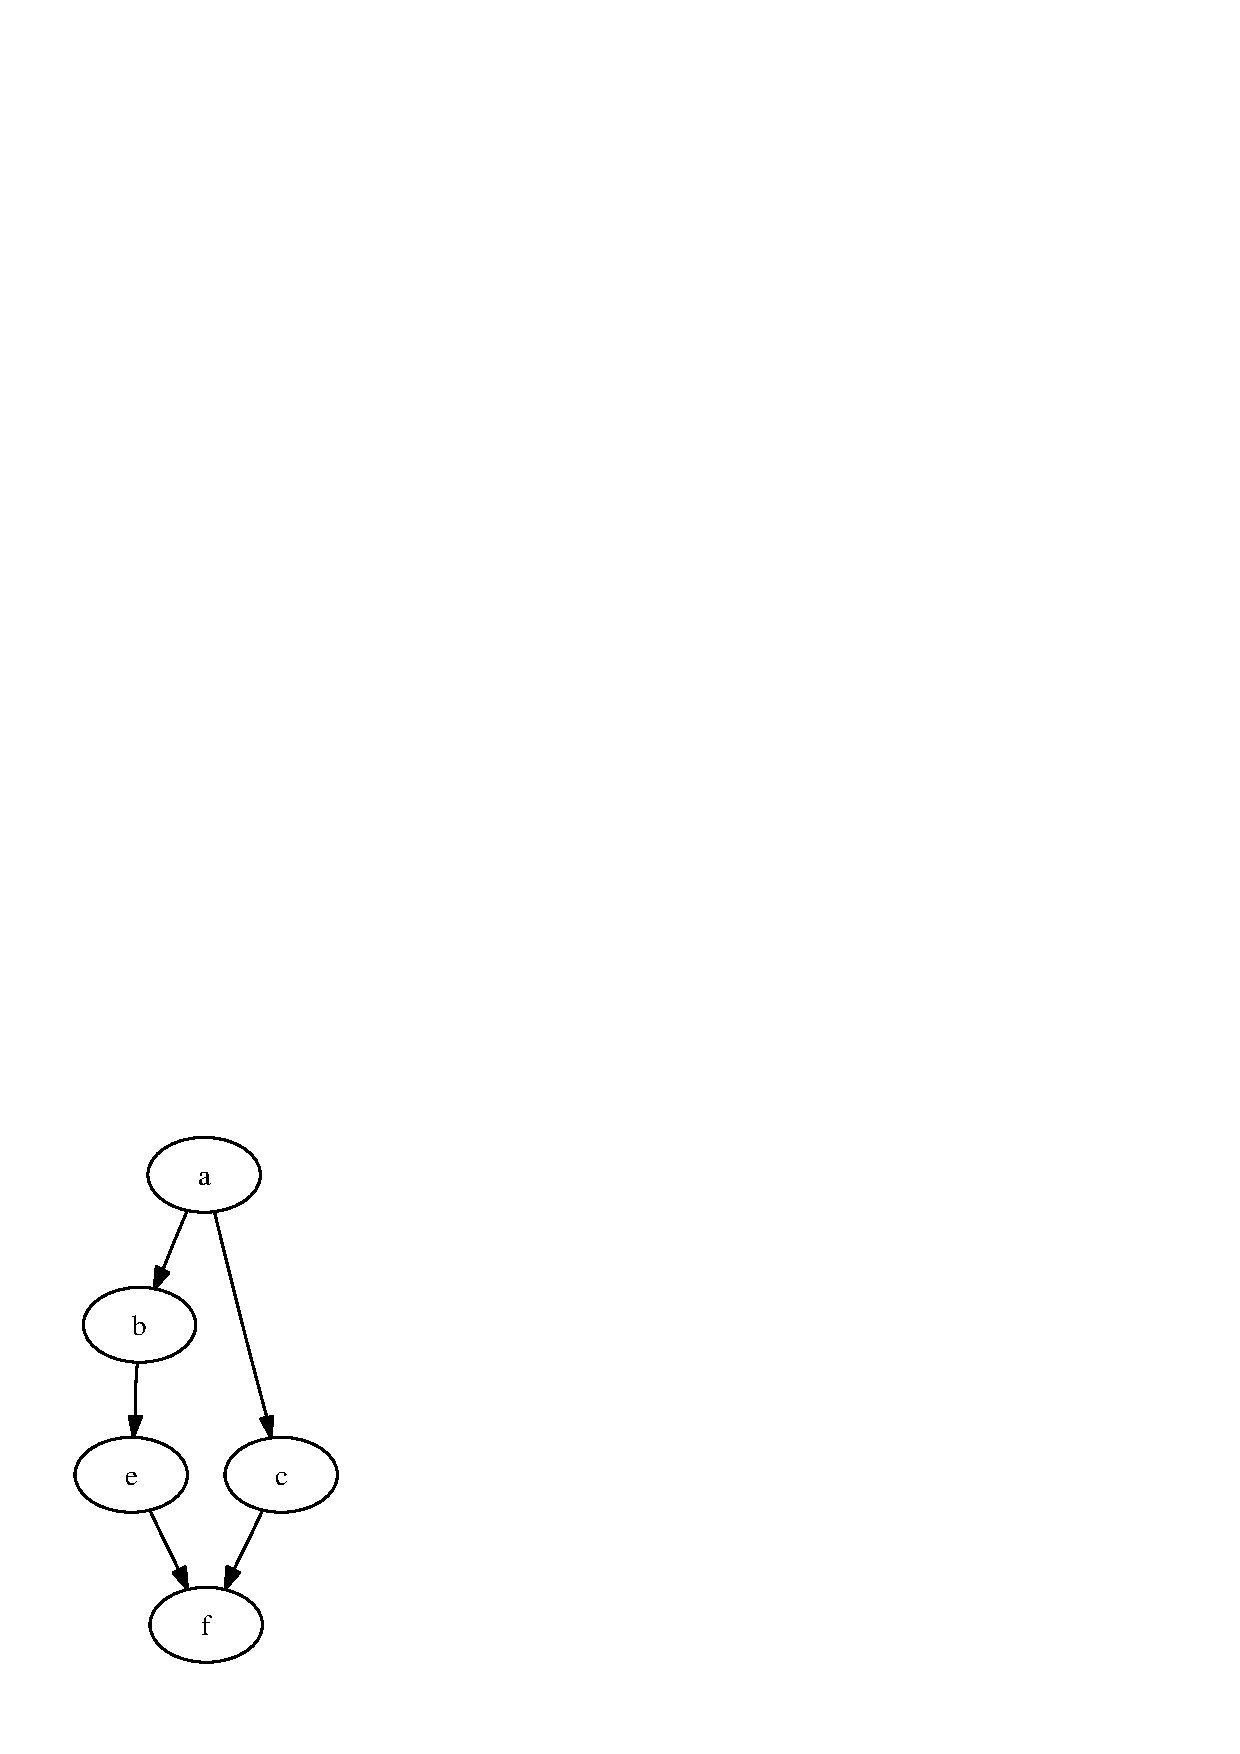
\epsfig{file=Figures/graph,scale=0.5}
  \caption{Ein einfacher Graph ohne Zykeln}
  \label{fig:graph}
\end{figure}

Wir wollen nun ein \textsl{Prolog}-Programm entwickeln, mit dem es m�glich ist, f�r zwei
vorgegebene Knoten $x$ und $y$ zu entscheiden, ob es einen Weg von $x$ nach $y$ gibt.
Au�erdem soll dieser Weg dann als Liste von Knoten berechnet werden.
Unser erster Ansatz besteht aus dem Programm, das in Abbildung \ref{fig:connect} gezeigt
ist.  Die Idee ist, dass der Aufruf \\[0.1cm]
\hspace*{1.3cm} \texttt{find\_path(\textsl{Start}, \textsl{Goal}, \textsl{Path})} \\[0.1cm]
einen Pfad \textsl{Path} berechnet, der von \textsl{Start} nach \textsl{Goal} f�hrt.  Wir diskutieren
die Implementierung.

\begin{figure}[!h]
  \centering
\begin{Verbatim}[ frame         = lines, 
                  framesep      = 0.3cm, 
                  labelposition = bottomline,
                  numbers       = left,
                  numbersep     = -0.2cm,
                  xleftmargin   = 0.8cm,
                  xrightmargin  = 0.8cm
                ]
    % find_path( +Point, +Point, -List(Point) ).
    find_path( X, X, [ X ] ).
    
    find_path( X, Z, [ X | Path ] ) :-
        edge( X, Y ),
        find_path( Y, Z, Path ).
\end{Verbatim}
\vspace*{-0.3cm}
  \caption{Berechnung von Pfaden in einem Graphen}
  \label{fig:connect}
\end{figure}

\begin{enumerate}
\item Die erste Klausel sagt aus, dass es trivialerweise einen Pfad von \texttt{X} nach
      \texttt{X} gibt.  Dieser Pfad enth�lt genau den Knoten \texttt{X}.
\item Die zweite Klausel sagt aus, dass es einen Weg von \texttt{X} nach \texttt{Z}
      gibt, wenn es zun�chst eine direkte Verbindung von \texttt{X} zu einem Knoten
      \texttt{Y} gibt und wenn es dann von diesem Knoten \texttt{Y} eine Verbindung
      zu dem Knoten \texttt{Z} gibt.  Wir erhalten den Pfad, der von \texttt{X} nach
      \texttt{Z} f�hrt, dadurch, dass wir vorne an den Pfad, der von \texttt{Y} nach \texttt{Z}
      f�hrt, den Knoten \texttt{X} anf�gen.
\end{enumerate}
Stellen wir an das \textsl{Prolog}-System die Anfrage \texttt{find\_path(a,f,P)}, so
erhalten wir die Antwort
\begin{Verbatim}[ frame         = lines, 
                  framesep      = 0.3cm, 
                  labelposition = bottomline,
                  numbers       = left,
                  numbersep     = -0.2cm,
                  xleftmargin   = 0.8cm,
                  xrightmargin  = 0.8cm
                ]
    ?- find_path(a,f,P).
 
    P = [a, b, e, f] ;   
    P = [a, c, f] ;
    No
\end{Verbatim}
Durch Backtracking werden also alle m�glichen Wege von \texttt{a} nach \texttt{b} gefunden.
Als n�chstes testen wir das Programm mit dem in Abbildung \ref{fig:graph2} gezeigten
Graphen.  Diesen Graphen stellen wir wie folgt in \textsl{Prolog} dar:
\begin{Verbatim}[ frame         = lines, 
                  framesep      = 0.3cm, 
                  labelposition = bottomline,
                  numbers       = left,
                  numbersep     = -0.2cm,
                  xleftmargin   = 0.8cm,
                  xrightmargin  = 0.8cm
                ]
    edge(a, b).
    edge(a, c).
    edge(b, e).
    edge(e, a).
    edge(e, f).
    edge(c, f).
\end{Verbatim}

\begin{figure}[!h]
  \centering
  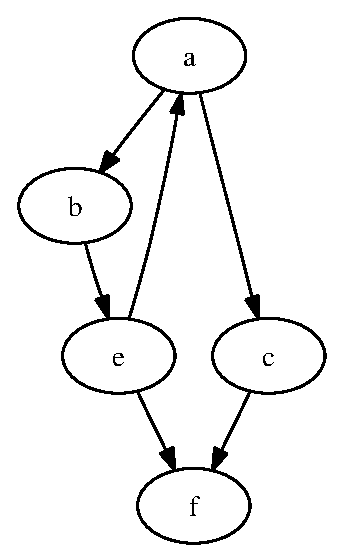
\epsfig{file=Figures/graph2,scale=0.5}
  \caption{Ein Graph mit einem Zykel}
  \label{fig:graph2}
\end{figure}

Jetzt erhalten wir auf die Anfrage \texttt{find\_path(a,f,P)} die Antwort
\begin{Verbatim}[ frame         = lines, 
                  framesep      = 0.3cm, 
                  labelposition = bottomline,
                  numbers       = left,
                  numbersep     = -0.2cm,
                  xleftmargin   = 0.8cm,
                  xrightmargin  = 0.8cm
                ]
    ?- find_path(a,f,P).
    ERROR: Out of local stack
\end{Verbatim}
Die Ursache ist schnell gefunden.
\begin{enumerate}
\item Wir starten mit der Anfrage \\[0.1cm]
      \hspace*{1.3cm} \texttt{find\_path(a,f,P)}.
\item Nach Unifikation mit der zweiten Klausel haben wir die Anfrage reduziert auf \\[0.1cm]
      \hspace*{1.3cm} 
      \texttt{edge( a, Y1 ), find\_path( Y1, f, P1 )}.
\item Nach Unifikation mit dem Fakt \texttt{edge(a,b)} haben wir die neue Anfrage \\[0.1cm]
      \hspace*{1.3cm} 
      \texttt{find\_path( b, f, P1 )}.
\item Nach Unifikation mit der zweiten Klausel haben wir die Anfrage reduziert auf \\[0.1cm]
      \hspace*{1.3cm} 
      \texttt{edge( b, Y2 ), find\_path( Y2, f, P2 )}.
\item Nach Unifikation mit dem Fakt \texttt{edge(b,e)} haben wir die neue Anfrage \\[0.1cm]
      \hspace*{1.3cm} 
      \texttt{find\_path( e, f, P2 )}.
\item Nach Unifikation mit der zweiten Klausel haben wir die Anfrage reduziert auf \\[0.1cm]
      \hspace*{1.3cm} 
      \texttt{edge( e, Y3 ), find\_path( Y3, f, P3 )}.
\item Nach Unifikation mit dem Fakt \texttt{edge(e,a)} haben wir die neue Anfrage \\[0.1cm]
      \hspace*{1.3cm} 
      \texttt{find\_path( a, f, P3 )}.
\end{enumerate}
Die Anfrage ``\texttt{find\_path(a, f, P3)}'' unterscheidet sich von der urspr�nglichen
Anfrage ``\texttt{find\_path(a,f,P)}'' nur durch den Namen der Variablen.  Wenn wir jetzt
weiterrechnen w�rden, w�rde sich die Rechnung nur wiederholen, ohne dass wir vorw�rts kommen.
Das Problem ist, das \textsl{Prolog} immer die erste
Klausel nimmt, die passt.  Wenn sp�ter die Reduktion der Anfrage scheitert, wird zwar nach
Backtracking die n�chste Klausel ausprobiert, aber wenn das Programm in eine
Endlos-Schleife l�uft, dann gibt es eben kein Backtracking, denn das Programm wei� ja
nicht, dass es in einer Endlos-Schleife ist.

Es ist leicht das Programm so umzuschreiben, dass keine Endlos-Schleife mehr
auftreten kann.  Die Idee ist, dass wir uns merken, welche Knoten wir bereits besucht
haben und diese nicht mehr ausw�hlen.  In diesem Sinne implementieren wir nun ein Pr�dikat \texttt{find\_path/4}.
Die Idee ist, dass der Aufruf \\[0.1cm]
\hspace*{1.3cm} \texttt{find\_path(\textsl{Start}, \textsl{Goal}, \textsl{Visited}, \textsl{Path})} \\[0.1cm]
einen Pfad berechnet, der von \textsl{Start} nach \textsl{Goal} f�hrt und der zus�tzlich
keine Knoten benutzt, die bereits in der Liste \textsl{Visited} aufgef�hrt sind.  Diese Liste
f�llen wir bei den rekursiven Aufrufen nach und nach mit den Knoten an, die wir bereits
besucht haben.  Mit Hilfe dieser Liste vermeiden wir es, einen Knoten zweimal zu besuchen.
Abbildung \ref{fig:connect2} zeigt die Implementierung.
\begin{figure}[!h]
  \centering
\begin{Verbatim}[ frame         = lines, 
                  framesep      = 0.3cm, 
                  labelposition = bottomline,
                  numbers       = left,
                  numbersep     = -0.2cm,
                  xleftmargin   = 0.8cm,
                  xrightmargin  = 0.8cm
                ]
    % find_path( +Point, +Point, +List(Point), -List(Point) )

    find_path( X, X, _Visited, [ X ] ).
    
    find_path( X, Z, Visited, [ X | Path ]) :-
        edge( X, Y ),
        \+ member( Y, Visited ),
        find_path( Y, Z, [ Y | Visited ], Path ).
    \end{Verbatim}
\vspace*{-0.3cm}
  \caption{Berechnung von Pfaden in zyklischen Graphen}
  \label{fig:connect2}
\end{figure}
\begin{enumerate}
\item In der ersten Klausel spielt das zus�tzliche Argument noch keine Rolle,
      denn wenn wir das Ziel erreicht haben, ist es uns egal, welche Knoten wir schon
      besucht haben.
\item In der zweiten Klausel �berpr�fen wir in Zeile 7, ob der Knoten \texttt{Y}
      in der Liste \textsl{Visited}, die die Knoten enth�lt, die bereits besucht wurden,
      auftritt.  Nur wenn dies nicht der Fall ist, versuchen wir rekursiv von \texttt{Y}
      einen Pfad nach \texttt{Z} zu finden.  Bei dem rekursiven Aufruf erweitern wir die Liste
      \texttt{Visited} um den Knoten \texttt{Y}, denn diesen Knoten wollen wir in Zukunft
      ebenfalls vermeiden.
\end{enumerate}
Mit dieser Implementierung ist es jetzt m�glich, auch in dem zweiten Graphen einen Weg von
\texttt{a} nach \texttt{f} zu finden, wir erhalten folgendes Ergebnis:
\pagebreak

\begin{Verbatim}[ frame         = lines, 
                  framesep      = 0.3cm, 
                  labelposition = bottomline,
                  numbers       = left,
                  numbersep     = -0.2cm,
                  xleftmargin   = 0.8cm,
                  xrightmargin  = 0.8cm
                ]
    ?- find_path(a,f,[a],P).
    P = [a, b, e, f] ;
    P = [a, c, f] ;    
    No
\end{Verbatim}


\subsection{Die Bekehrung der Ungl�ubigen}
Als spielerische Anwendung zeigen wir nun, wie sich mit Hilfe des oben definierten Pr�dikats 
\texttt{find\_path/4} ein theologisches Problem l�sen l�sst.
\vspace*{0.3cm}

\begin{minipage}[c]{14cm}
{\sl Drei Missionare und drei Ungl�ubige wollen zusammen einen Fluss 
�berqueren. Sie haben nur ein Boot, indem maximal zwei Passagiere fahren k�nnen.  
Sowohl die Ungl�ubigen als auch die Missionare k�nnen rudern.
Weder die Gl�ubigen, noch die Ungl�ubigen k�nnen �ber das Wasser laufen.
Die Ungl�ubigen sind hungrig, wenn die Missionare an einem der Ufer in der Unterzahl sind, 
haben sie ein Problem.  Die Aufgabe besteht darin, einen Fahrplan zu 
erstellen, so dass hinterher alle das andere  Ufer erreichen und die
Missionare zwischendurch kein Problem haben.}
\end{minipage}
\vspace*{0.4cm}

\noindent
Die Idee ist, das R�tsel, durch einen Graphen zu modellieren.  Die Knoten dieses 
Graphen sind dann die Situationen, die w�hrend des �bersetzens auftreten.  Wir
repr�sentieren diese Situationen durch Terme der Form \\[0.1cm]
\hspace*{1.3cm} $\texttt{side}(M,\;K,\;B)$.
\\[0.1cm]
Ein solcher Term repr�sentiert eine Situation, bei der auf der linken Seite des Ufers $M$ Missionare, $K$
Ungl�ubige und $B$ Boote sind.  Unsere Aufgabe besteht nun darin, das Pr�dikat
\texttt{edge/2} so zu implementieren, dass \\[0.1cm]
\hspace*{1.3cm} $\texttt{edge}(\;\texttt{side}(M_1,\;K_1,\;B_1),\;\texttt{side}(M_2,\;K_2,\;B_2)\;)$
\\[0.1cm]
genau dann wahr ist, wenn die Situation $\texttt{side}(M_1,\;K_1,\;B_1)$
durch eine Boots-�berfahrt in die Situation $\texttt{side}(M_2,\;K_2,\;B_2)$ �berf�hrt
werden kann und wenn zus�tzlich die Missionare in der neuen Situation kein Problem bekommen.
Abbildung \ref{fig:missionare.pl} auf Seite \pageref{fig:missionare.pl}
zeigt ein \textsl{Prolog}-Programm, was das R�tsel l�st.  Den von diesem Programm
berechneten Fahrplan finden Sie in Abbildung \ref{fig:missionare-solution} 
auf Seite \pageref{fig:missionare-solution}.
Wir diskutieren dieses Programm nun Zeile f�r Zeile.

\begin{figure}[!h]
  \centering
\begin{Verbatim}[ frame         = lines, 
                  framesep      = 0.3cm, 
                  labelposition = bottomline,
                  numbers       = left,
                  numbersep     = -0.2cm,
                  xleftmargin   = 0.8cm,
                  xrightmargin  = 0.8cm
                ]
    MMM   KKK   B      |~~~~~|                   
                       >  KK >
    MMM   K            |~~~~~|      B    KK      
                       <  K  <
    MMM   KK    B      |~~~~~|            K      
                       >  KK >
    MMM                |~~~~~|      B   KKK      
                       <  K  <
    MMM   K     B      |~~~~~|           KK      
                       > MM  >
    M     K            |~~~~~|      B    KK    MM
                       < M K <
    MM    KK    B      |~~~~~|            K     M
                       > MM  >
          KK           |~~~~~|      B     K   MMM
                       <  K  <
          KKK   B      |~~~~~|                MMM
                       >  KK >
          K            |~~~~~|      B    KK   MMM
                       <  K  <
          KK    B      |~~~~~|            K   MMM
                       >  KK >
                       |~~~~~|      B   KKK   MMM
\end{Verbatim}
\vspace*{-0.3cm}
  \caption{Fahrplan f�r Missionare und Ungl�ubige}
  \label{fig:missionare-solution}
\end{figure}      

\begin{figure}[!h]
  \centering
\begin{Verbatim}[ frame         = lines, 
                  framesep      = 0.3cm, 
                  labelposition = bottomline,
                  numbers       = left,
                  numbersep     = -0.2cm,
                  xleftmargin   = 0.8cm,
                  xrightmargin  = 0.8cm
                ]
    solve :-
        find_path( side(3,3,1), side(0,0,0), [ side(3,3,1) ], Path ),
        nl, write('L�sung:' ), nl, nl,
        print_path(Path).
    
    % edge( +Point, -Point ).    
    % This clause describes rowing from the left side to the right side.
    edge( side( M, K, 1 ), side( MN, KN, 0 ) ) :-
        between( 0, M, MB ),    % MB missionaries in the boat
        between( 0, K, KB ),    % KB infidels in the boat
        MB + KB >= 1,           % boat must not be empty
        MB + KB =< 2,           % no more than two passengers
        MN is M - MB,           % missionaries left on the left side
        KN is K - KB,           % infidels left on the left side
        \+ problem( MN, KN ).   % no problem must occur
    
    % This clause describes rowing from the right side to the left side.
    edge( side( M, K, 0 ), side( MN, KN, 1 ) ) :-
        otherSide( M, K, MR, KR ),
        edge( side( MR, KR, 1 ), side( MRN, KRN, 0 ) ),
        otherSide( MRN, KRN, MN, KN ).
    
    % otherSide( +Number, +Number, -Number, -Number ).
    otherSide( M, K, M_Other, K_Other ) :-
        M_Other is 3 - M,
        K_Other is 3 - K.
    
    % problem( +Number, +Number).
    problem(M, K) :- 
            problemSide(M, K).
    
    problem(M, K) :-
        otherSide( M, K, M_Other, K_Other ),
        problemSide(M_Other, K_Other).
        
    % problemSide( +Number, +Number).
    problemSide(Missionare, Kannibalen) :- 
            Missionare > 0, 
            Missionare < Kannibalen.
    
    % find_path( +Point, +Point, +List(Point), -List(Point) )
    find_path( X, X, _Visited, [ X ] ).
    
    find_path( X, Z, Visited, [ X | Path ]) :-
            edge( X, Y ),
            \+ member( Y, Visited ),
            find_path( Y, Z, [ Y | Visited ], Path ).
\end{Verbatim}
\vspace*{-0.3cm}
  \caption{Die Bekehrung der Ungl�ubigen}
  \label{fig:missionare.pl}
\end{figure}      

\begin{enumerate}
\item Wir beginnen mit dem  Hilfs-Pr�dikat \texttt{otherSide/4}, das in den
      Zeilen 24 -- 26 implementiert ist.  F�r eine vorgegebene Situation
      $\texttt{side}(M,K,B)$ berechnet der Aufruf \\[0.1cm]
      \hspace*{1.3cm} $\texttt{otherSide}(\; \texttt{side}(M, K, B),\; \textsl{OtherSide} \;)$
      \\[0.1cm] 
      einen Term, der die Situation am gegen�berliegenden Ufer beschreibt.
      Wenn an einen Ufer $M$ Missionare sind, so sind am anderen Ufer die restlichen
      Missionare und da es insgesamt $3$ Missionare gibt, sind das $3 - M$.
      Die Anzahl der Ungl�ubige am gegen�berliegenden Ufer wird analog berechnet. 
\item Das Pr�dikat \texttt{problem/2} in den Zeilen 29 -- 34 �berpr�ft, ob es bei einer vorgegeben
      Anzahl von Missionaren und Ungl�ubige zu einem Problem kommt.
      Da das Problem entweder am linken oder am rechten Ufer auftreten kann,
      besteht die Implementierung aus zwei Klauseln.  Die erste Klausel pr�ft,
      ob es auf der Seite, an der $M$ Missionare und $K$ Ungl�ubige sind, zum Problem
      kommt.  Die zweite Klausel �berpr�ft, ob es auf dem gegen�berliegenden
      Ufer zu einem Problem kommt.  Als Hilfs-Pr�dikat verwenden wir hier das Pr�dikat
      \texttt{problemSide/2}.  Dieses Pr�dikat ist in Zeile 37 implementiert
      und �berpr�ft die Situation an einer Seite:  Falls sich auf einer Seite $M$ Missionare
      und $K$ Ungl�ubige befinden, so gibt es dann ein Problem, wenn die Zahl $M$ von 0
      verschieden ist und wenn zus�tzlich $M < K$ ist.
\item Bei der Implementierung des Pr�dikats \texttt{edge/2} verwenden wir in den Zeilen 9
      und 10 das Pr�dikat \texttt{between/3}, das in dem \textsl{SWI-Prolog}-System 
      vordefiniert ist.  Beim Aufruf \\[0.1cm]
      \hspace*{1.3cm} $\texttt{between}(\textsl{Low}, \textsl{High}, N)$ \\[0.1cm]
      sind \textsl{Low} und \textsl{High} ganze Zahlen mit $\textsl{Low} \leq \textsl{High}$.
      Der Aufruf instantiert die Variable $N$ nacheinander mit den Zahlen \\[0.1cm]
      \hspace*{1.3cm} $\textsl{Low},\; \textsl{Low}+1,\; \textsl{Low}+2, \cdots, \;\textsl{High}$. \\[0.1cm]
      Beispielsweise gibt die Anfrage \\[0.1cm]
      \hspace*{1.3cm} \texttt{between(1,3,N), write(N), nl, fail.}  \\[0.1cm]
      nacheinander die Zahlen 1, 2 und 3 am Bildschirm aus.
    \item Die Implementierung des Pr�dikats \texttt{edge/2} besteht aus zwei Klauseln.  In
      der ersten Klausel betrachten wir den Fall, dass das Boot am linken Ufer ist.  In
      der Zeilen 9 generieren wir die Zahl der Missionare $\texttt{MB}$, die im Boot �bersetzen
      sollen.  Diese Zahl $\texttt{MB}$ ist durch $\texttt{M}$ beschr�nkt, denn es k�nnen nur die Missionare
      �bersetzen, die sich am linken Ufer befinden.  Daher benutzen wir das Pr�dikat
      \texttt{between/3} um eine Zahl zwischen 0 und $\texttt{M}$ zu erzeugen.  Analog generieren
      wir in Zeile 10 die Zahl $\texttt{KB}$ der Ungl�ubige, die im Boot �bersetzen.  In Zeile 11
      testen wir, dass es mindestens einen Passagier gibt, der mit dem Boot �bersetzt und
      in Zeile 12 testen wir, dass es h�chstens zwei Passagiere sind.  In Zeile 13 und 14
      berechnen wir die Zahl $\texttt{MN}$ der Missionare und die Zahl $\texttt{KN}$ der Ungl�ubige, die
      nach der �berfahrt auf dem linken Ufer verbleiben und testen dann in Zeile 15, dass es
      f�r diese Zahlen kein Problem gibt.
      
      Die zweite Klausel befasst sich mit dem Fall, dass das Boot am rechten Ufer liegt.
      Wir h�tten diese Klausel mit \textsl{Copy \& Paste} aus der vorhergehenden Klausel
      erzeugen k�nnen, aber es ist eleganter, diesen Fall auf den vorhergehenden Fall
      zur�ck zu f�hren.  Da da Boot nun auf der rechten Seite liegt, berechnen wir daher
      in Zeile 19 die Zahl $\texttt{MR}$ der Missionare auf der rechten Seite und die Zahl
      $\texttt{KR}$ der Ungl�ubige auf der rechten Seite.  Dann untersuchen wir die
      Situation $\mathtt{side}(\mathtt{MR}, \mathtt{KR}, 1)$, bei der $\texttt{MR}$
      Missionare und $\texttt{KR}$ Ungl�ubige am linken Ufer stehen.  Wenn diese so
      �bersetzen k�nnen, dass nachher $\texttt{MRN}$ Missionare und $\texttt{KRN}$
      Ungl�ubige am linken Ufer stehen, dann k�nnen wir in Zeile 21 berechnen, wieviele
      Missionare und Ungl�ubige sich dann am gegen�berliegenden Ufer befinden.
\item In den Zeilen 1 -- 4 definieren wir nun das Pr�dikat \texttt{solve/0}, dessen Aufruf
      das Problem l�st.  Dazu wird zun�chst das Pr�dikat \texttt{find\_path/4} 
      mit dem Start-Knoten \texttt{side(3,3,1)} und dem Ziel-Knoten \texttt{side(0,0,0)}
      aufgerufen.   Der berechnete Pfad wird dann ausgegeben mit dem Pr�dikat
      \texttt{print\_path/1},
      dessen Implementierung hier aus Platzgr�nden nicht angegeben wird.
\end{enumerate}


%%% Local Variables: 
%%% mode: latex
%%% TeX-master: "logik"
%%% End: 

%\section{Der Cut-Operator}
Wir haben ein Pr�dikat als \emph{funktional} definiert,
wenn wir die einzelnen Argumente klar in Eingabe- und Ausgabe-Argumente
aufteilen k�nnen.  Wir nennen ein Pr�dikat \emph{deterministisch} wenn es funktional ist
und wenn au�erdem zu jeder Eingabe h�chstens eine Ausgabe berechnet
wird.  Diese zweite Forderung ist durchaus nicht immer erf�llt.  Betrachten wir die ersten
beiden Fakten zur Definition des Pr�dikats \texttt{mix/3}:
\begin{Verbatim}[ frame         = lines, 
                  framesep      = 0.3cm, 
                  labelposition = bottomline,
                  numbers       = left,
                  numbersep     = -0.2cm,
                  xleftmargin   = 0.8cm,
                  xrightmargin  = 0.8cm
                ]
    mix( [], Xs, Xs ).    
    mix( Xs, [], Xs ).
\end{Verbatim}
F�r die Anfrage ``\texttt{mix([], [], L)}'' k�nnen beide Fakten verwendet werden.
Das Ergebnis ist zwar immer das selbe, n�mlich \texttt{L = []}, es wird aber zweimal ausgegeben:
\begin{Verbatim}[ frame         = lines, 
                  framesep      = 0.3cm, 
                  labelposition = bottomline,
                  numbers       = left,
                  numbersep     = -0.2cm,
                  xleftmargin   = 0.8cm,
                  xrightmargin  = 0.8cm
                ]
    ?- mix([],[],L).
    
    L = [] ;
    
    L = [] 
\end{Verbatim}
Dies kann zu Ineffizienz f�hren.  Aus diesem Grunde gibt es in \textsl{Prolog} den
Cut-Operator ``\texttt{!}''.  Mit diesem Operator ist es m�glich, redundante L�sungen aus
dem Suchraum heraus zu schneiden.  Schreiben wir die ersten beiden Klauseln der
Implementierung von \texttt{mix/3} in der Form 
\begin{Verbatim}[ frame         = lines, 
                  framesep      = 0.3cm, 
                  labelposition = bottomline,
                  numbers       = left,
                  numbersep     = -0.2cm,
                  xleftmargin   = 0.8cm,
                  xrightmargin  = 0.8cm
                ]
    mix( [], Xs, Xs ) :- !.
    mix( Xs, [], Xs ) :- !.
\end{Verbatim}
so wird auf die Anfrage  ``\texttt{mix([], [], L)}'' die L�sung \texttt{L = []} nur noch
einmal generiert.  Ist allgemein eine Regel der Form \\[0.1cm]
\hspace*{1.3cm} $P \;\texttt{:-}\; Q_1, \cdots, Q_m, \texttt{!}, R_1, \cdots, R_k$ \\[0.1cm]
gegeben, und gibt es weiter eine Anfrage $A$, so dass $A$ und $P$  unifizierbar sind, so
wird die Anfrage $A$ zun�chst zu der Anfrage \\[0.1cm]
\hspace*{1.3cm} $Q_1\mu, \cdots, Q_m\mu, \texttt{!}, R_1\mu, \cdots, R_k\mu$ \\[0.1cm]
reduziert.  Au�erdem wird ein Auswahl-Punkt gesetzt, wenn es noch weitere Klauseln gibt,
deren Kopf mit $A$ unifiziert werden k�nnt.
Bei der weiteren Abarbeitung dieser Anfrage gilt folgendes:
\begin{enumerate}
\item Falls bereits die Abarbeitung einer Anfrage der Form \\[0.1cm]
      \hspace*{1.3cm} 
      $Q_i\sigma, \cdots, Q_m\sigma, \texttt{!}, R_1\sigma, \cdots, R_k\sigma$ \\[0.1cm]
      f�r ein $i\in\{1,\cdots,m\}$ scheitert, so wird der Cut nicht erreicht und hat keine
      Wirkung.
\item Eine Anfrage der Form \\[0.1cm]
      \hspace*{1.3cm} 
      $\texttt{!}, R_1\sigma, \cdots, R_k\sigma$ \\[0.1cm]
      wird reduziert zu \\[0.1cm]
      \hspace*{1.3cm} 
      $R_1\sigma, \cdots, R_k\sigma$. \\[0.1cm]
      Dabei werden alle Auswahl-Punkte, die bei der Beantwortung der Teilanfragen
      $Q_1, \cdots, Q_m$ gesetzt worden sind, gel�scht.  Au�erdem wird ein eventuell bei
      der Reduktion der Anfrage $A$ auf die Anfrage \\[0.1cm]
      \hspace*{1.3cm} $Q_1\mu, \cdots, Q_m\mu, \texttt{!}, R_1\mu, \cdots, R_k\mu$
      \\[0.1cm]
      gesetzter Auswahl-Punkte gel�scht.
\item Sollte sp�ter die Beantwortung der Anfrage \\[0.1cm]
      \hspace*{1.3cm} $R_1\sigma, \cdots, R_k\sigma$. \\[0.1cm]
      scheitern, so scheitert auch die Beantwortung der Anfrage $A$.
\end{enumerate}
Zur Veranschaulichung betrachten wir ein Beispiel.
\begin{Verbatim}[ frame         = lines, 
                  framesep      = 0.3cm, 
                  labelposition = bottomline,
                  numbers       = left,
                  numbersep     = -0.2cm,
                  xleftmargin   = 0.8cm,
                  xrightmargin  = 0.8cm
                ]
    q(Z) :- p(Z).
    q(1).

    p(X) :- a(X), b(X), !, c(X,Y), d(Y).    
    p(3).
    
    a(1).    a(2).    a(3).
    
    b(2).    b(3).
    
    c(2,2).  c(2,4).
    
    d(3).
\end{Verbatim}
Wir verfolgen die Beantwortung der Anfrage \ \texttt{q(U)}. 
\begin{enumerate}
\item Zun�chst wird versucht \texttt{q(U)} mit dem Kopf der ersten Klausel 
      des Pr�dikats \texttt{q/1}  zu unifizieren.  Dabei wird \texttt{Z} mit
      \texttt{U} instantiert und die Anfrage wird reduziert zu \\[0.1cm]
      \hspace*{1.3cm} \texttt{p(U)}. \\[0.1cm]
      Da es noch eine weiter Klausel f�r das Pr�dikat \texttt{q/1} gibt, die zur
      Beantwortung der Anfrage q(U) in Frage kommt, setzen wir Auswahl-Punkt Nr.~1.
\item Jetzt wird versucht \texttt{p(U)} mit \texttt{p(X)} zu unifizieren.  Dabei
      wird die Variable \texttt{X} an \texttt{U} gebunden und die urspr�ngliche Anfrage
      wird reduziert zu der Anfrage \\[0.1cm]
      \hspace*{1.3cm}  
      \texttt{a(U), b(U), !, c(U,Y), d(Y)}. \\[0.1cm]
      Au�erdem wird an dieser Stelle Auswahl-Punkt Nr.~2 gesetzt, denn die zweite Klausel
      des Pr�dikats \texttt{p/1} kann ja ebenfalls mit der urspr�nglichen Anfrage unifiziert
      werden. 
\item Um die Teilanfrage \texttt{a(U)} zu beantworten, wird \texttt{a(U)} mit
      \texttt{a(1)} unifiziert.  Dabei wird \texttt{U} mit 1 instantiiert und die Anfrage wird reduziert zu \\[0.1cm]
      \hspace*{1.3cm} 
      \texttt{b(1), !, c(1,Y), d(Y)}. \\[0.1cm]
      Da es f�r das Pr�dikat \texttt{a/1} noch weitere Klauseln gibt, wird Auswahl-Punkt Nr.~3
      gesetzt.
\item Jetzt wird versucht, die Anfrage \\[0.1cm]
      \hspace*{1.3cm}    \texttt{b(1), !, c(1,Y), d(Y)}. \\[0.1cm]
      zu l�sen.  Dieser Versuch scheitert jedoch, da sich die f�r das Pr�dikat \texttt{b/1}
      vorliegenden Fakten nicht mit \texttt{b(1)} unifizieren lassen.
\item Also springen wir zur�ck zum letzten Auswahl-Punkt (das ist Auswahl-Punkt Nr.~3)
      und machen die Instantiierung 
      $\texttt{U} \mapsto 1$ r�ckg�ngig.  Wir haben jetzt also wieder das Ziel \\[0.1cm]
      \hspace*{1.3cm} \texttt{a(U), b(U), !, c(U,Y), d(Y)}. 
\item Diesmal w�hlen wir das Fakt \texttt{a(2)} um es mit \texttt{a(U)} zu unifizieren.  Dabei wird \texttt{U} mit
      2 instantiiert und wir haben die  Anfrage \\[0.1cm]
      \hspace*{1.3cm} \texttt{b(2), !, c(2,Y), d(Y)}. \\[0.1cm]
      Da es noch eine weiter Klausel f�r das Pr�dikat \texttt{a/1} gibt, setzen wir 
      Auswahl-Punkt Nr.~4 an dieser Stelle.
\item Jetzt unifizieren wir  die Teilanfrage \texttt{b(2)} mit der ersten Klausel f�r das Pr�dikat
      \texttt{b/1}.  Die verbleibende Anfrage ist \\[0.1cm]
      \hspace*{1.3cm} \texttt{!, c(2,Y), d(Y)}. 
\item Diese Anfrage wird reduziert zu \\[0.1cm]
      \hspace*{1.3cm}  \texttt{c(2,Y), d(Y)}. \\[0.1cm]
      Au�erdem werden bei diesem Schritt die Auswahl-Punkte Nr.~2 und Nr.~4 gel�scht.
\item Um diese Anfrage zu beantworten, unifizieren wir \texttt{c(2,Y)} mit dem Kopf der
      ersten Klausel f�r das Pr�dikat \texttt{c/2}, also mit \texttt{c(2,2)}.
      Dabei erhalten wir die Instantiierung
      $\mathtt{Y} \mapsto 2$.  Die Anfrage ist damit reduziert zu \\[0.1cm]
      \hspace*{1.3cm}  \texttt{d(2)}. \\[0.1cm]
      Au�erdem setzen wir an dieser Stelle Auswahl-Punkt Nr.~5, denn das Pr�dikat
      \texttt{c/2} hat ja noch eine weitere Klausel, die in Frage kommt.
\item Die Anfrage ``\texttt{d(2)}'' scheitert.  Also springen wir zur�ck zum Auswahl-Punkt
      Nr.~5 und machen die Instantiierung $\mathtt{Y} \mapsto 2$ r�ckg�ngig.  Wir haben
      also wieder die Anfrage \\[0.1cm]
      \hspace*{1.3cm}  \texttt{c(2,Y), d(Y)}. 
\item Zur Beantwortung dieser Anfrage nehmen wir nun die zweite Klausel der
      Implementierung von \texttt{c/2} und erhalten die Instantiierung 
      $\mathtt{Y} \mapsto 4$.  Die verbleibende Anfrage lautet dann \\[0.1cm]
      \hspace*{1.3cm} \texttt{d(4)}.
\item Da sich \texttt{d(4)} und \texttt{d(3)} nicht unifizieren lassen,
      scheitert diese Anfrage.  Wir springen jetzt zur�ck zum Auswahl-Punkt Nr.~1 und
      machen die Instantiierung $\mathtt{U} \mapsto \mathtt{Z}$ r�ckg�ngig.  Die Anfrage
      lautet also wieder \\[0.1cm]
      \hspace*{1.3cm} \texttt{p(U)}.
\item W�hlen wir nun die zweite Klausel der Implementierung von \texttt{q/1},
      so m�ssen wir \texttt{q(U)} und \texttt{q(1)} unifizieren.  Diese Unifikation ist
      erfolgreich und wir erhalten die Instantiierung $\mathtt{U} \mapsto 1$, die die Anfrage beantwortet.
\end{enumerate}

\subsection{Verbesserung der Effizienz von \textsl{Prolog}-Programmen durch den Cut-Operator}
In der Praxis wird der Cut-Operator eingesetzt, um �berfl�ssige Auswahl-Punkte zu
entfernen und dadurch die Effizienz eines Programms zu steigern.  Als Beispiel
betrachten wir eine Implementierung des Algorithmus 
``\emph{Sortieren durch Vertauschen}'' (engl.~\emph{bubble sort}).
Wir spezifizieren diesen Algorithmus zun�chst durch bedingte Gleichungen.  Dabei 
benutzen wir die Funktion \\[0.1cm]
\hspace*{1.3cm} 
$\texttt{append}: \textsl{List}(\textsl{Number}) \times \textsl{List}(\textsl{Number}) \rightarrow \textsl{List}(\textsl{Number})$
\\[0.1cm]
Der Aufruf $\texttt{append}(l_1, l_2)$ liefert eine Liste, die aus allen Elementen von
$l_1$ gefolgt von den Elementen aus $l_2$ besteht.  In dem \textsl{SWI-Prolog}-System ist
ein entsprechendes Pr�dikat \texttt{append/3} implementiert.  Die Implementierung dieses
Pr�dikats deckt sich mit der Implementierung des Pr�dikats \texttt{concat/3}, die wir in
einem fr�heren Abschnitt vorgestellt hatten.  

Au�erdem benutzen wir noch das Pr�dikat \\[0.1cm]
\hspace*{1.3cm} 
$\texttt{ordered}: \textsl{List}(\textsl{Number}) \rightarrow \mathbb{B}$, \\[0.1cm]
das �berpr�ft, ob eine Liste geordnet ist.
Die bedingten Gleichungen
zur Spezifikation der Funktion \\[0.1cm]
\hspace*{1.3cm} 
$\texttt{bubble\_sort}: \textsl{List}(\textsl{Number}) \rightarrow \textsl{List}(\textsl{Number})$
\\[0.1cm]
lauten nun:
\begin{enumerate}
\item $\mathtt{append}(l_1, [x,y|l_2], l) \wedge x > y \rightarrow \mathtt{bubble\_sort}(l) = \mathtt{bubble\_sort}(\mathtt{append}(l_1, [y,x|l_2]))$

      Wenn die Liste $l$ in zwei Teile $l_1$ und $[x,y|l_2]$ zerlegt werden kann
      und wenn weiter $x>y$ ist, dann vertauschen wir die Elemente $x$ und $y$
      und sortieren die so entstandene Liste rekursiv.
\item $\mathtt{ordered}(l) \rightarrow \mathtt{bubble\_sort}(l) = l$

      Wenn die Liste $l$ bereits sortiert ist, dann kann die Funktion
      $\mathtt{bubble\_sort}$ diese Liste unver�ndert als Ergebnis zur�ck geben.
\end{enumerate}
Die Gleichungen um das Pr�dikat \texttt{ordered} zu spezifizieren lauten:
\begin{enumerate}
\item $\mathtt{ordered}([]) = \mathtt{true}$

      Die leere Liste ist offensichtlich sortiert.
\item $\mathtt{ordered}([x]) = \mathtt{true}$

      Eine Liste, die nur aus einem Element besteht, ist ebenfalls sortiert.
\item $x \leq y \rightarrow \mathtt{ordered}([x,y|r]) = \mathtt{ordered}([y|r])$.

      Eine Liste der Form $[x,y|r]$ ist sortiert, wenn $x \leq y$ ist und
      wenn au�erdem die Liste $[y|r]$ sortiert ist.
\end{enumerate}

\begin{figure}[!h]
  \centering
\begin{Verbatim}[ frame         = lines, 
                  framesep      = 0.3cm, 
                  labelposition = bottomline,
                  numbers       = left,
                  numbersep     = -0.2cm,
                  xleftmargin   = 0.8cm,
                  xrightmargin  = 0.8cm
                ]
    bubble_sort( L, Sorted ) :-
        append( L1, [ X, Y | L2 ], L ),
        X > Y,
        append( L1, [ Y, X | L2 ], Cs ),
        bubble_sort( Cs, Sorted ).
    
    bubble_sort( Sorted, Sorted ) :-
        is_ordered( Sorted ).
    
    
    is_ordered( [] ).
    
    is_ordered( [ _ ] ).
    
    is_ordered( [ X, Y | Ys ] ) :-
        X < Y,
        is_ordered( [ Y | Ys ] ).
\end{Verbatim}
\vspace*{-0.3cm}
  \caption{Der Bubble-Sort Algorithmus}
  \label{fig:bubble_sort}
\end{figure}

Abbildung \ref{fig:bubble_sort} zeigt die Implementierung des Bubble-Sort Algorithmus in
\textsl{Prolog}.  In Zeile 2 wird die als Eingabe gegebene Liste \texttt{L} in die beiden
Liste \texttt{L1} und \texttt{[X, Y | L2]} zerlegt.  Da es im Allgemeinen mehrere
M�glichkeiten gibt,  eine Liste in zwei Teillisten zu zerlegen, wird hierbei ein
Auswahl-Punkt gesetzt.  Anschlie�end wird gepr�ft, ob \texttt{Y} kleiner als \texttt{X}
ist.  Wenn dies der Fall ist, wird mit \texttt{append/3} die neue Liste 
\\[0.1cm]
\hspace*{1.3cm} $\mathtt{append(L_1, [Y,X|L_2])}$ \\[0.1cm]
gebildet und diese Liste wird rekuriv sortiert.  Wenn es nicht m�glich ist,
die Liste \texttt{L} so in zwei Listen \texttt{L1} und \texttt{[X, Y | L2]} zu zerlegen,
dass \texttt{Y} kleiner als \texttt{X} ist, dann muss die Liste \texttt{L} schon sortiert
sein.  In diesem Fall greift die zweite Klausel, die allerdings noch �berpr�fen muss, ob
\texttt{L} tats�chlich sortiert ist, denn sonst k�nnte beim Backtracking eine falsche
L�sung berechnet werden.

Das Problem bei dem obigen Programm ist die Effizienz.  Aufgrund der vielen M�glichkeiten
eine Liste zu zerlegen, wird beim Backtracking immer wieder die selbe L�sung generiert. 
Beispielsweise liefert die Anfrage \\[0.1cm]
\hspace*{1.3cm} \texttt{bubble\_sort( [ 4, 3, 2, 1 ], L ), write(L), nl, fail.} \\[0.1cm]
16 mal die selbe L�sung.  Abbildung \ref{fig:bubble_sort_cut} zeigt eine Implementierung,
bei der nur eine L�sung berechnet wird.  Dies wird durch den Cut-Operator in Zeile 4
erreicht.   Ist einmal eine Zerlegung der Liste \texttt{L} der Form
\\[0.2cm]
\hspace*{1.3cm}
$\mathtt{L} = \texttt{L}_1 +[ \texttt{X}, \mathtt{Y} | \mathtt{L}_2]$
\\[0.2cm] 
gefunden, bei der \texttt{Y} kleiner als \texttt{X} ist, so bringt es
nichts mehr, nach anderen Zerlegungen zu suchen, denn die urspr�nglich gegebene Liste
\texttt{L} l��t sich ja auf jeden Fall dadurch sortieren, dass rekursiv die Liste 
\\[0.2cm]
\hspace*{1.3cm}
 $\mathtt{L}_1 + [\mathtt{Y},\mathtt{X}|\mathtt{L}_2]$ 
\\[0.1cm]
sortiert wird.  Dann kann auch der Aufruf der Pr�dikats \texttt{ordered/1} im Rumpf der zweiten
Klausel des Pr�dikats \texttt/2{bubble\_sort} entfallen, denn diese wird beim Backtracking
ja nur dann erreicht, wenn es keine Zerlegung der Liste \texttt{L} in  \texttt{L1} und 
\texttt{[X, Y | L2]} gibt, bei der \texttt{Y} kleiner als \texttt{X} ist.  Dann mu� aber
die Liste \texttt{L} schon sortiert sein.

\begin{figure}[!h]
  \centering
\begin{Verbatim}[ frame         = lines, 
                  framesep      = 0.3cm, 
                  labelposition = bottomline,
                  numbers       = left,
                  numbersep     = -0.2cm,
                  xleftmargin   = 0.8cm,
                  xrightmargin  = 0.8cm
                ]
    bubble_sort( List, Sorted ) :-
        append( L1, [ X, Y | L2 ], List ),
        X > Y,
        !,
        append( L1, [ Y, X | L2 ], Cs ),
        bubble_sort( Cs, Sorted ).
    
    bubble_sort( Sorted, Sorted ).
\end{Verbatim}
\vspace*{-0.3cm}
  \caption{Effiziente Implementierung des  Bubble-Sort Algorithmus}
  \label{fig:bubble_sort_cut}
\end{figure}

Wenn wir bei der Entwicklung eines \textsl{Prolog}-Programms von bedingten Gleichungen
ausgehen, dann gibt es ein einfaches Verfahren, um das entstandene
\textsl{Prolog}-Programm durch die Einf�hrung von Cut-Operator effizienter zu machen:
Der Cut-Operator sollte nach den Tests, die vor dem Junktor ``$\rightarrow$'' stehen,
gesetzt werden.  Wir erl�utern dies durch ein Beispiel:  Unten sind noch einmal die
Gleichungen zur Spezifikation des Algorithmus ``\emph{Sortieren durch Mischen}'' wiedergegeben.
\begin{enumerate}
\item $\mathtt{odd}([]) = []$.
\item $\mathtt{odd}([h|t]) = [h|\mathtt{even}(t)]$.
\item $\mathtt{even}([]) = []$.
\item $\mathtt{even}([h|t]) = \mathtt{odd}(t)$.
\item $\mathtt{merge}([], l) = l$.
\item $\mathtt{merge}(l, []) = l$.
\item $x \leq y \rightarrow \mathtt{merge}([x|s], [y|t]) = [x|\mathtt{merge}(s, [y|t])]$.
\item $x  >   y \rightarrow \mathtt{merge}([x|s], [y|t]) = [y|\mathtt{merge}([x|s], t)]$.
\item $\mathtt{sort}([]) = []$.
\item $\mathtt{sort}([x]) = [x]$.
\item $\mathtt{sort}([x,y|t]) = \mathtt{merge}( \mathtt{sort}(\mathtt{odd}([x,y|t])), \mathtt{sort}(\mathtt{even}([x,y|t])))$.
\end{enumerate}
Das \textsl{Prolog}-Programm mit Cut-Operatoren sieht dann so aus wie in Abbildung
\ref{fig:merge-sort-cut} gezeigt.  Nur die Gleichungen 7.~und 8.~haben Bedingungen, bei
allen anderen Gleichungen gibt es keine Bedingungen.  Bei den Gleichungen 7.~und 8.~wird
der Cut-Operator daher nach dem Test der Bedingungen gesetzt, bei allen anderen Klauseln
wird der Cut-Operator dann am Anfang des Rumpfes gesetzt.

\begin{figure}[!h]
  \centering
\begin{Verbatim}[ frame         = lines, 
                  framesep      = 0.3cm, 
                  labelposition = bottomline,
                  numbers       = left,
                  numbersep     = -0.2cm,
                  xleftmargin   = 0.8cm,
                  xrightmargin  = 0.8cm
                ]
    % odd( +List(Number), -List(Number) ).    
    odd( [], [] ) :- !.    
    odd( [ X | Xs ], [ X | L ] ) :-
        !,
        even( Xs, L ).

    % even( +List(Number), -List(Number) ).
    even( [], [] ) :- !.
    even( [ _X | Xs ], L ) :-
        !,
        odd( Xs, L ).
    
    % merge( +List(Number), +List(Number), -List(Number) ).
    mix( [], Xs, Xs ) :- !.    
    mix( Xs, [], Xs ) :- !.
    mix( [ X | Xs ], [ Y | Ys ], [ X | Rest ] ) :-
        X =< Y,
        !,
        mix( Xs, [ Y | Ys ], Rest ).
    mix( [ X | Xs ], [ Y | Ys ], [ Y | Rest ] ) :-
        X > Y,
        !,
        mix( [ X | Xs ], Ys, Rest ).
    
    % merge_sort( +List(Number), -List(Number) ).
    merge_sort( [], [] ) :- !.
    merge_sort( [ X ], [ X] ) :- !.
    merge_sort( [ X, Y | Rest ], Sorted ) :-
        !,
        odd(  [ X, Y | Rest ], Odd  ),
        even( [ X, Y | Rest ], Even ),
        merge_sort( Odd,  Odd_Sorted  ),
        merge_sort( Even, Even_Sorted ),
        mix( Odd_Sorted, Even_Sorted, Sorted ).
\end{Verbatim}
\vspace*{-0.3cm}
  \caption{Sortieren durch Mischen mit Cut-Operatoren.}
  \label{fig:merge-sort-cut}
\end{figure}

Analysieren wir das obige Programm genauer, so stellen wir fest, dass viele der
Cut-Operatoren im Grunde �berfl�ssig sind.  Beispielsweise kann immer nur eine der beiden
Klauseln, die das Pr�dikat \texttt{odd/2} implementieren, greifen, denn entweder ist die
eingegebene Liste leer oder nicht.  Also sind die Cut-Operatoren in den Zeilen 2 und 4
redundant.  Andererseits st�ren sie auch nicht, so dass es f�r die Praxis das einfachste
sein d�rfte Cut-Operatoren stur nach dem oben angegebenen Rezept zu setzen.
\pagebreak

\vspace*{\fill}

\section{Literaturhinweise}
F�r eine umfangreiche und dem Thema angemessene Darstellung der Sprache \textsl{Prolog} 
fehlt in der einf�hrenden Vorlesung leider die Zeit.  Daher wird dieses Thema in einer
sp�teren Vorlesung auch wieder aufgegriffen.  Den Lesern, die ihre Kenntnisse jetzt schon
vertiefen wollen, m�chte ich die folgende Hinweise auf die Literatur geben:
\begin{enumerate}
\item \emph{The Art of Prolog} von Leon Sterling und Ehud Shapiro \cite{sterling:94}.
      Dieses Werk ist ein ausgezeichnete Lehrbuch, das auch f�r den Anf�nger gut lesbar ist.
\item \emph{Prolog Programming for Artificial Intelligence} von Ivan Bratko
      \cite{bratko:90}.  Neben der Sprache \textsl{Prolog} f�hrt dieses Buch auch in die
      k�nstliche Intelligenz ein.
\item \emph{Foundations of Logic Programnming}   von J.~W.~Lloyd \cite{lloyd:87}
      beschreibt die theoretischen Grundlagen der Sprache \textsl{Prolog}.
\item \emph{Prolog: The Standard} von Pierre Deransart, Abdel Ali Ed-Dbali und Laurent
      Cervoni \cite{deransart:96} gibt den ISO-Standard f�r die Sprache
      \textsl{Prolog} wieder.
\item \emph{SWI-Prolog 6.2.6 Reference Manual} von Jan Wielemaker \cite{wielemaker:2013}
      beschreibt das SWI-Prolog-System.  Dieses Dokument ist im Internet unter der Adresse 
      \\[0.1cm]
      \hspace*{1.3cm}      
      \href{http://www.swi-prolog.org/download/stable/doc/SWI-Prolog-6.2.6.pdf}{\texttt{http://www.swi-prolog.org/download/stable/doc/SWI-Prolog-6.2.6.pdf}}
      \\[0.1cm]
      verf�gbar.
\end{enumerate}

%%% Local Variables: 
%%% mode: latex
%%% TeX-master: "logik"
%%% End: 



\bibliographystyle{alpha}
\bibliography{cs}

\end{document}



%%% Local Variables: 
%%% mode: latex
%%% TeX-master: "logik"
%%% End: 
